\documentclass{book}

%\overfullrule=4bp

\usepackage{url}
\newcommand{\pclURL}[2]{\href{#1}{#2}\footnote{\href{#1}{#1.}}}

\usepackage[utf8]{inputenc}
\usepackage[T2A]{fontenc}
\usepackage[russian]{babel}
\usepackage{fancyvrb}
\usepackage[dvips]{color}
\usepackage{stmaryrd}
\usepackage{tabularx,mdwtab}
%\usepackage{needspace}
\usepackage{indentfirst}
\usepackage{longtable,citehack,enumerate}
\usepackage{marginnote}
\usepackage{array}
\usepackage{ifmtarg}
\usepackage{centernot}
\usepackage{empheq}
\usepackage{needspace}
\usepackage{colonequals}
\usepackage[nottoc]{tocbibind}
\usepackage{emptypage}

\usepackage{makeidx}
\makeindex

%\usepackage{fancybox}
%% Я хотел использовать fancybox ради \ovalbox, но он определяет свой
%% собственный Verbatim, который конфликтует с fancyvrb.
%% В конце концов нужно будет либо выдернуть оттуда определение
%% \ovalbox, либо отказаться от fancyvrb. Пока что я просто не делаю
%% круглых углов.
\newcommand{\ovalbox}[1]{\fbox{#1}}

%\usepackage[unicode,colorlinks=true]{hyperref}
\usepackage[unicode,]{hyperref}
%\usepackage{hyperref}
%\definecolor{pfpcolorint}{rgb}{0,0.4,0}
%\definecolor{pfpcolorext}{rgb}{0,0,0.6}
%\definecolor{pfpcolorint}{gray}{0.9}
%\definecolor{pfpcolorext}{gray}{0.9}

\hypersetup{%colorlinks,
%	linkcolor=pfpcolorint,
%	citecolor=pfpcolorint,
%	filecolor=pfpcolorext,
%	urlcolor=pfpcolorext,
	bookmarksopen,bookmarksopenlevel=0,
	pdffitwindow,
        colorlinks=false,
        pdfborder={0 0 0},
	% pdfsubject={},
	% pdfkeywords={}
	pdftitle={Practical Common Lisp}
}

\usepackage{epigraph}

\beforeepigraphskip 0pt plus 1fill

% 70х100/16 -> 170mmх240mm
 \usepackage[papersize={160mm,220mm},asymmetric,% bindingoffset=5mm,
hmargin={1cm,1cm},vmargin={1cm,1cm},includehead,ignorefoot,heightrounded,headsep=12bp,headheight=12.5bp,footnotesep=10bp plus2bp minus2bp]{geometry}

% headers & footers
%% \usepackage{fancyhdr}
%% \pagestyle{fancy}
%\include{version}
%% \fancyhead{}
%% \fancyhead[RE,LO]{\slshape{\rightmark{}}}
%% \fancyhead[LE,RO]{\thepage{}}
%\fancyfoot{}
%\fancyfoot[LE,RO]{rev. \svnInfoMaxRevision}
% 
\usepackage{graphicx}

\usepackage[round]{natbib}
\bibliographystyle{plainnat}
\renewcommand{\cite}{\citep} % ???? citep*
\newcommand{\citeterse}{\citep}
\newcommand{\citeyr}[1]{(\citeyear{#1})}
\newcommand{\citeyropen}[1]{\citeyear{#1}}
\newcommand{\longcite}[1]{\citeauthor{#1} \citeyearpar{#1}}
\newcommand{\fulllongcite}[1]{\citeauthor*{#1} \citeyearpar{#1}}
\newcommand{\citeopen}[1]{\citealp{#1}} % citealp*
\newcommand{\citeopenterse}[1]{\citealp{#1}}

\usepackage{bold-extra}
\usepackage{listings}
\definecolor{listingcomment}{gray}{0.3}
\lstset{%
  language=lisp,
  basicstyle=\footnotesize\upshape,%\ttfamily,
  keywordstyle=\bfseries,
  showtabs=false, 
  showspaces=false, 
  showstringspaces=false,% OK?
  tabsize=2,
  commentstyle=\color{listingcomment},
  extendedchars=\true{},
  mathescape=\true{},% allows to use math symbols in listings - may be
                     % dangerous
  basewidth={.5em,.5em},% columns=fullflexible
  xleftmargin=.943em,
  morekeywords={IF, LET, QUOTE, EQ, EQL, EQUAL, EQUALP, NIL, T, FORMAT, if, LOAD, DOLIST,
    PRINT, LIST, DEFUN}
}
\lstdefinestyle{lisp}{language=Lisp,keywordstyle=\bfseries}

% TODO: decrease space before/after myverb...
\usepackage{alltt}
\newenvironment{myverb}[0]{\begin{alltt}\footnotesize}{\end{alltt}}
\newcommand\bslash{\symbol{`\\}}

\lstdefinestyle{lisprepl}{keywords={}}

\DeclareRobustCommand{\code}[1]{\texttt{\small\texorpdfstring{\def\ldots{...}%
\spaceskip\codespaceskip\relax}{}% \spaceskip3bp plus 1.5bp minus1bp\relax 
#1}}
\def\codespaceskip{\the\spaceskip}
\newcommand{\stdcode}[1]{\code{#1}}
\newcommand{\keyword}[1]{\code{\textbf{#1}}}

%% proper captions for figures, etc
\usepackage{caption}

% Добавляем точку после номера раздела
\usepackage{titlesec}
\titlelabel{\thetitle.\quad}
\usepackage[dotinlabels]{titletoc}

% TODO: remove the page number from chapter page
% http://stackoverflow.com/questions/2166557/how-to-hide-the-page-number-in-latex-on-first-page-of-a-chapter
% http://tex.stackexchange.com/questions/88833/page-number-on-the-first-page-of-chapter

% settings for floating objects
\renewcommand{\topfraction}{.9}
\renewcommand{\textfraction}{.1}
\renewcommand{\bottomfraction}{.9}
\setcounter{totalnumber}{2}

\fboxsep.25em
\definecolor{gray}{gray}{0.75}
\newcommand{\graybg}[1]{\colorbox{gray}{\mbox{#1}}}

\makeatletter
\newcommand{\translationnotemark}{{\renewcommand{\@makefnmark}{*}\footnotemark{}}}
\newcommand{\translationnotetext}[1]{{\renewcommand{\@makefnmark}{*}\footnotetext{#1 \@Acdash \emph{Прим. перев.}}}\addtocounter{footnote}{-1}}
\newcommand{\translationnote}[1]{\translationnotemark{}\translationnotetext{\hspace{1mm}#1}}
\newcommand{\unmarkednote}[1]{{\renewcommand{\@makefnmark}{}\footnotemark{}\footnotetext{#1}}\addtocounter{footnote}{-1}}
\makeatother

\newcommand\nextpage{\emph{См. след. страницу}}


\title{Practical Common Lisp}
\author{Peter Seibel}

%\usepackage{sections}

\makeatletter
\renewcommand\@makefnmark{\mbox{\textsuperscript{\normalfont\@thefnmark}\hspace{1mm}}}
\makeatother

\begin{document}
% Don't remove! used for tikz nodes align!
\newlength{\tikztextheight}\settoheight{\tikztextheight}{!}

\VerbatimFootnotes

\selectlanguage{russian}%
\frenchspacing
\righthyphenmin=2

%% TODO: remove...
\sloppy

\frontmatter

\makeatletter
\@nameuse{ttl@ps@\string\chapter}
\makeatother

%%% здесь можно комментировать одно и раскомментировать другое, чтобы
%%% быстро тестировать компиляцию по главам
%\chapter{Не только списки: другие применения cons-ячеек}
\label{ch:13}

Как вы увидели в предыдущей главе, списочный тип данных является иллюзией, созданной
множеством функций, которые манипулируют cons-ячейками. Common Lisp также предоставляет
функции, позволяющие вам обращаться со структурами данных, созданными из cons-ячеек, как c
деревьями, множествами и таблицами поиска (\textit{lookup tables}). В этой главе я дам
вам краткий обзор некоторых из этих структур данных и оперирующих с ними функций. Как и в
случае функций, работающих со списками, многие из них будут полезны, когда вы начнёте
писать более сложные макросы, где потребуется обращаться с кодом Lisp как с данными.


\section{Деревья}

Рассматривать структуры, созданные из cons-ячеек, как деревья так же естественно, как
рассматривать их как списки. Ведь что такое список списков, как не другое представление
дерева?  Разница между функцией, которая обращается с группой cons-ячеек как со списком, и
функцией, обращающейся с той же группой cons-ячеек как с деревом, определяется тем, какие
ячейки обходят эти функции при поиске значений для дерева или списка. Те сons-ячейки,
которые обходит функция работы со списком, называются \textit{списочной структурой}
(\textit{list structure}) и
располагаются, начиная от первой cons-ячейки и затем следуя ссылкам по \lstinline{CDR}, пока не
достигнут \lstinline{NIL}.  Элементами списка являются объекты, на которые ссылаются
\lstinline{CAR}'ы cons-ячеек списочной структуры. Если cons-ячейка в списочной структуре имеет
\lstinline{CAR}, который ссылается на другую cons-ячейку, то та ячейка, на которую ведёт
ссылка, считается головой и элементом внешнего списка\footnote{Возможно создать цепь
  списочных ячеек, где \lstinline{CDR} последней ячейки будет не \lstinline{NIL}, а неким другим
  атомом. Такая конструкция будет называться \textit{точечным списком} (\textit{dotted
    list}), потому что последняя списочная ячейка является точечной парой.}.
\textit{Древовидная структура} (\textit{tree structure}), с другой стороны, при обходе следует
ссылкам как по \lstinline{CAR}, так и по \lstinline{CDR}, пока они указывают на другие cons-ячейки. Таким
образом, значениями в древовидной структуре являются атомы~-- такие значения, которые не
являются cons-ячейками и на которые ссылаются \lstinline{CAR}'ы или \lstinline{CDR}'ы cons-ячеек в
древовидной структуре.

Например, следующая стрелочная диаграмма показывает cons-ячейки, составляющие список из
списков: \lstinline{((1 2) (3 4) (5 6))}. Списочная структура включает в себя только три
cons-ячейки внутри пунктирного блока, тогда как древовидная структура включает все ячейки.

%TODO: add picture
%{{ pcl:chapter13:ch13-1.png }}

Чтобы увидеть разницу между функцией, работающей со списком, и функцией, работающей с
деревом, вы можете рассмотреть, как функции \lstinline{COPY-LIST} и \lstinline{COPY-TREE} будут
копировать эту группу cons-ячеек. \lstinline{COPY-LIST} как функция, работающая со списком,
копирует cons-ячейки, которые составляют списочную структуру. Другими словами, она создаёт
новые cons-ячейки соответственно для каждой из cons-ячеек пунктирного блока. \lstinline{CAR}'ы
каждой новой ячейки ссылаются на тот же объект, что и \lstinline{CAR}'ы оригинальных cons-ячеек
в списочной структуре. Таким образом, \lstinline{COPY-LIST} не копирует подсписки
\lstinline{(1, 2)}, \lstinline{(3 4)}, или \lstinline{(5 6)}, как показано на этой диаграмме:

%TODO: add picture
%{{ pcl:chapter13:ch13-2.png }}

\lstinline{COPY-TREE}, с другой стороны, создаёт новые cons-ячейки для каждой из cons-ячеек на
диаграмме и соединяет их вместе в одну структуру, как показано на следующей диаграмме:

%TODO: add picture
%{{ pcl:chapter13:ch13-3.png }}

Там, где cons-ячейки в оригинале ссылаются на атомарное значение, соответствующие им
cons-ячейки в копии будут ссылаться на то же значение.  Таким образом, единственными
объектами, на которые ссылаются как оригинальное дерево, так и его копия, созданная
\lstinline{COPY-TREE}, будут числа \lstinline{5}, \lstinline{6} и символ \lstinline{NIL}.

Еще одна функция, которая обходит как \lstinline{CAR}'ы, так и \lstinline{CDR}'ы cons-ячеек дерева,~--
это \lstinline{TREE-EQUAL}, которая сравнивает два дерева и считает их равными, если их
структуры имеют одинаковую форму и если их листья равны относительно \lstinline{EQL} (или если
они удовлетворяют условию, задаваемому через именованный аргумент \lstinline{:test}).

Прочими ориентированными на деревья функциями являются работающие с деревьями аналоги
функций для последовательностей \lstinline{SUBSTITUTE} и \lstinline{NSUBSTITUTE}, а также их \lstinline{-IF} и
\lstinline{-IF-NOT} варианты. Функция \lstinline{SUBST}, как и \lstinline{SUBSTITUTE}, принимает новый
элемент, старый элемент и дерево (в отличие от последовательности) вместе с именованными
аргументами \lstinline{:key} и \lstinline{:test} и возвращает новое дерево с той же формой, что и
исходное, но все вхождения старого элемента заменяются новым. Например:

\begin{myverb}
  CL-USER> (subst 10 1 '(1 2 (3 2 1) ((1 1) (2 2))))
  (10 2 (3 2 10) ((10 10) (2 2)))
\end{myverb}

\lstinline{SUBST-IF} аналогична \lstinline{SUBSTITUTE-IF}. Но вместо старого элемента она принимает
одноаргументную функцию, которая вызывается с аргументом в виде каждого атомарного
значения в дереве, и всякий раз, когда она возвращает истину, текущая позиция в новом
дереве заменяется новым значением. \lstinline{SUBST-IF-NOT} действует так же, за исключением
того, что заменяются те значения, где функция возвращает \lstinline{NIL}. \lstinline{NSUBST},
\lstinline{NSUBST-IF}, и \lstinline{NSUBST-IF-NOT}~-- это утилизирующие аналоги соответствующих
версий \lstinline{SUBST}-функций. Как и с другими утилизирующими функциями, вам следует
использовать эти функции только как замещение (после профилирования) их неразрушающих
аналогов в ситуациях, где вы уверены, что нет опасности повреждения разделяемой
структуры. В частности, вы должны продолжать сохранять возвращаемые значения этих функций,
пока у вас нет гарантии, что результат будет равен, по предикату \lstinline{EQ}, оригинальному
дереву\footnote{Казалось бы, семейство \lstinline{NSUBST}-функций не только может, но и в
  действительности модифицирует дерево прямо на месте. Однако имеется один крайний случай:
  когда переданное <<дерево>> фактически является атомом, оно не может быть модифицировано
  по месту, тогда результатом NSUBST будет являться отличный от аргумента объект:
  \lstinline!(nsubst 'x 'y 'y) X!.}.

\section{Множества}

Множества также могут быть реализованы посредством cons-ячеек. Фактически вы можете
обращаться с любым списком как со множеством~-- Common Lisp предоставляет несколько функций
для выполнения теоретико-множественных операций над списками. Тем не менее вам следует
помнить, что из-за особенности устройства списков эти операции становятся тем менее и
менее эффективными, чем больше становится множество.

Впрочем, используя встроенные функции для работы со множествами, легко писать оперирующий со
множествами код. И для небольших множеств они могут быть более эффективными, чем их
альтернативы. Если профилирование показывает вам, что производительность этих функций
является узким местом вашего кода, вы всегда можете заменить множества на основе списков
множествами, основанными на хэш-таблицах или битовых векторах.

Для создания множества вы можете использовать функцию \lstinline{ADJOIN}. \lstinline{ADJOIN}
принимает в качестве аргументов элемент и список, представляющий множество, и возвращает
список, содержащий этот элемент вместе со всеми элементами исходного множества.  Для того
чтобы определить, присутствует ли элемент во множестве, функция просматривает список, и
если элемент не найден, то \lstinline{ADJOIN} создаёт новую cons-ячейку, содержащую этот
элемент, ссылающуюся на исходный список, и возвращает её. В противном случае она
возвращает исходный список.

\lstinline{ADJOIN} также принимает именованные аргументы \lstinline{:key} и \lstinline{:test}, которые
используются при определении, присутствует ли элемент в исходном списке. Подобно
\lstinline{CONS}, \lstinline{ADJOIN} не воздействует на исходный список~-- если вы хотите
модифицировать определённый список, вам нужно присвоить значение, возвращаемое
\lstinline{ADJOIN}, тому месту, в котором хранился исходный список. Неразрушающий макрос
\lstinline{PUSHNEW} сделает это для вас автоматически.

\begin{myverb}
  CL-USER> (defparameter *set* ())
  *SET*
  CL-USER> (adjoin 1 *set*)
  (1)
  CL-USER> *set*
  NIL
  CL-USER> (setf *set* (adjoin 1 *set*))
  (1)
  CL-USER> (pushnew 2 *set*)
  (2 1)
  CL-USER> *set*
  (2 1)
  CL-USER> (pushnew 2 *set*)
  (2 1)
\end{myverb}

Вы можете проверить, принадлежит ли данный элемент множеству, с помощью функции
\lstinline{MEMBER} и родственных ей функций \lstinline{MEMBER-IF} и \lstinline{MEMBER-IF-NOT}. Эти
функции похожи на функции для работы с последовательностями \lstinline{FIND}, \lstinline{FIND-IF}
и \lstinline{FIND-IF-NOT}, за исключением того, что они используются только со списками. Вместо
того чтобы вернуть элемент, когда он присутствует во множестве, они возвращают cons-ячейку,
содержащую элемент, другими словами, подсписок, начинающийся с заданного элемента. Если
искомый элемент отсутствует в списке, все три функции возвращают \lstinline{NIL}.

Оставшиеся ориентированные на множества функции предоставляют операции с группами
элементов: \lstinline{INTERSECTION}, \lstinline{UNION}, \lstinline{SET-DIFFERENCE} и
\lstinline{SET-EXCLUSIVE-OR}.  Каждая из этих функций принимает два списка и именованные
аргументы \lstinline{:key} и \lstinline{:test} и возвращает новый список, представляющий множество,
полученное выполнением соответствующей операции над двумя списками. \lstinline{INTERSECTION}
возвращает список, содержащий все аргументы из обоих списков. \lstinline{UNION} возвращает
список, содержащий один экземпляр каждого уникального элемента из двух своих
аргументов\footnote{\lstinline{UNION} принимает только один элемент из каждого списка, но если
  один из двух списков содержит дублирующиеся элементы, результат может также содержать
  дубликаты.}. \lstinline{SET-DIFFERENCE} возвращает список, содержащий все элементы из первого
аргумента, которые не встречаются во втором аргументе. И \lstinline{SET-EXCLUSIVE-OR}
возвращает список, содержащий элементы, находящиеся только в одном либо в другом списках,
переданных в качестве аргументов, но не в обоих одновременно. Каждая из этих функций также
имеет утилизирующий аналог, имя которого получается добавлением \textit{N} в качестве
префикса.

В заключение функция \lstinline{SUBSETP} принимает в качестве аргументов два списка и обычные
именованные аргументы \lstinline{:key} и \lstinline{:test} и возвращает истину, если первый список
является подмножеством второго~-- то есть если каждый элемент первого списка также
присутствует во втором списке.  Порядок элементов в списках значения не имеет.

\begin{myverb}
  CL-USER> (subsetp '(3 2 1) '(1 2 3 4))
  T
  CL-USER> (subsetp '(1 2 3 4) '(3 2 1))
  NIL
\end{myverb}


\section{Таблицы поиска: ассоциативные списки и списки свойств}

Помимо деревьев и множеств, вы можете создавать таблицы, которые отображают ключи на
значения вне cons-ячеек. Обычно используются две разновидности основанных на cons-ячейках
таблиц поиска, об обеих я вскользь упоминал в предыдущих главах. Это \textit{ассоциативные
  списки} (\textit{association lists} или \textit{alists}) и \textit{списки свойств}
(\textit{property lists} или \textit{plists}). Вам не стоит использовать списки свойств
или ассоциативные списки для больших таблиц~-- для них нужно использовать хэш-таблицы, но
стоит знать, как работать с ними обоими, так как для небольших таблиц они могут быть более
эффективны, чем хэш-таблицы, и ещё потому, что у них есть несколько полезных собственных
свойств.
 
Ассоциативный список~-- это структура данных, которая отображает ключи на значения, а также
поддерживает обратный поиск, находя ключ по заданному значению. Ассоциативные списки также
поддерживают возможность добавления отображений ключ/значение, которые скрывают
существующие отображения таким образом, что скрывающие отображения могут быть позже
удалены и первоначальные отображения снова станут видимы.

Если смотреть глубже, то на самом деле ассоциативный список~-- это просто список, чьи
элементы сами является cons-ячейками. Каждый элемент можно представлять как пару
ключ/значение с ключом в \lstinline{CAR} cons-ячейки и значением в \lstinline{CDR}. К примеру,
следующая стрелочная диаграмма представляет ассоциативный список, состоящий из отображения
символа \lstinline{A} в номер \lstinline{1}, \lstinline{B} в номер \lstinline{2} и \lstinline{C} в номер \lstinline{3}:

%TODO: add picture
%{{ pcl:chapter13:ch13-4.png }}

Если значение \lstinline{CDR} не является списком, то cons-ячейки, представляющие пары ключ/значение,
будут \textit{точечными парами} (\textit{dotted pairs}) в терминах s-выражений. Ассоциативный
список, представленный на предыдущей диаграмме, к примеру, будет напечатан вот так:

\begin{myverb}
  ((A . 1) (B . 2) (C . 3))
\end{myverb}

Главная процедура поиска для ассоциативных списков~-- это \lstinline{ASSOC}, которая принимает
ключ и ассоциативный список в качестве аргументов и возвращает первую cons-ячейку, чей
\lstinline{CAR} соответствует ключу или является \lstinline{NIL}, если совпадения не найдено.
  
\begin{myverb}
  CL-USER> (assoc 'a '((a . 1) (b . 2) (c . 3)))
  (A . 1)
  CL-USER> (assoc 'c '((a . 1) (b . 2) (c . 3)))
  (C . 3)
  CL-USER> (assoc 'd '((a . 1) (b . 2) (c . 3)))
  NIL
\end{myverb}

Чтобы получить значение, соответствующее заданному ключу, вам следует просто передать
результат \lstinline{ASSOC} \lstinline{СDR}'у.
  
\begin{myverb}
  CL-USER> (cdr (assoc 'a '((a . 1) (b . 2) (c . 3))))
  1
\end{myverb}

По умолчанию заданный ключ сравнивается с ключами в ассоциативном списке, используя
предикат \lstinline{EQL}, но вы можете изменить его с помощью стандартной комбинации из
именованных аргументов \lstinline{:key} и \lstinline{:test}. Например, если вы хотите использовать
строковые ключи, то можете написать так:
  
\begin{myverb}
  CL-USER> (assoc "a" '(("a" . 1) ("b" . 2) ("c" . 3)) :test #'string=)
  ("a" . 1)
\end{myverb}

Без явного задания в качестве \lstinline{:test} предиката \lstinline{STRING=} \lstinline{ASSOC}, вероятно,
вернул бы \lstinline{NIL}, потому что две строки с одинаковым содержимым необязательно равны
относительно \lstinline{EQL}.

\begin{myverb}
  CL-USER> (assoc "a" '(("a" . 1) ("b" . 2) ("c" . 3)))
  NIL
\end{myverb}

Поскольку при поиске \lstinline{ASSOC} просматривает список с начала, одна пара ключ/значение в
ассоциативном списке может скрывать другие пары с тем же ключом, но находящиеся дальше в
списке.

\begin{myverb}
  CL-USER> (assoc 'a '((a . 10) (a . 1) (b . 2) (c . 3)))
  (A . 10)
\end{myverb}

Вы можете добавить пару в начало списка с помощью функции \lstinline{CONS}, как здесь:

\begin{myverb}
  (cons (cons 'new-key 'new-value) alist)
\end{myverb}

Однако для удобства Common Lisp предоставляет функцию \lstinline{ACONS}, которая позволяет вам
написать так:

\begin{myverb}
  (acons 'new-key 'new-value alist)
\end{myverb}

Подобно \lstinline{CONS}, \lstinline{ACONS} является функцией и, следовательно, не может
модифицировать место, откуда был передан исходный ассоциативный список. Если вы хотите
модифицировать ассоциативный список, вам нужно написать так:

\begin{myverb}
  (setf alist (acons 'new-key 'new-value alist))
\end{myverb}

\noindent{}или так:

\begin{myverb}
  (push (cons 'new-key 'new-value) alist)
\end{myverb}

Очевидно, время, затраченное на поиск в ассоциативном списке при использовании
\lstinline{ASSOC}, является функцией от того, насколько глубоко в списке находится
соответствующая пара. В худшем случае для определения, что никакая пара не соответствует
искомой, \lstinline{ASSOC} требуется просмотреть каждый элемент списка. Тем не менее поскольку
основной механизм работы ассоциативных списков довольно прост, то на небольших таблицах
ассоциативный список может превзойти в производительности хэш-таблицу.  Также
ассоциативные списки могут дать вам большую гибкость при выполнении поиска. Ранее я
отмечал, что \lstinline{ASSOC} принимает именованные аргументы \lstinline{:key} и \lstinline{:test}. Если
они не соответствуют вашим требованиям, вы можете использовать функции \lstinline{ASSOC-IF} и
\lstinline{ASSOC-IF-NOT}, которые возвращают первую пару ключ/значение, чей \lstinline{CAR}
удовлетворяет (или не удовлетворяет, в случае \lstinline{ASSOC-IF-NOT}) предикату,
передаваемому вместо ключа. Ещё три функции~-- \lstinline{RASSOC}, \lstinline{RASSOC-IF} и
\lstinline{RASSOC-IF-NOT}~-- действуют так же, как и соответствующие аналогичные
\lstinline{ASSOC}-функции, за исключением того, что они используют значение в \lstinline{CDR}
каждого элемента как ключ, совершая обратный поиск.

Функция \lstinline{COPY-ALIST} похожа на \lstinline{COPY-TREE}, за исключением того, что вместо
копирования всей древовидной структуры она копирует только те cons-ячейки, которые
составляют списочную структуру, плюс те cons-ячейки, на которые ссылаются \lstinline{CAR}'ы
этих ячеек. Другими словами, исходный ассоциативный список и его копия будут оба содержать
одинаковые объекты как в виде ключей, так и значений, даже если ключи или значения будут
состоять из cons-ячеек.

Наконец, вы можете создать ассоциативный список из двух различных списков ключей и значений
с помощью функции \lstinline{PAIRLIS}. Получившийся ассоциативный список может содержать пары
либо в том порядке, в каком они были в исходных списках, либо в обратном
порядке. Например, вы можете получить такой результат:

\begin{myverb}
  CL-USER> (pairlis '(a b c) '(1 2 3))
  ((C . 3) (B . 2) (A . 1))
\end{myverb}

Или вы можете получить следующее:

\begin{myverb}
  CL-USER> (pairlis '(a b c) '(1 2 3))
  ((A . 1) (B . 2) (C . 3))
\end{myverb}

Другой разновидностью таблицы поиска является список свойств (property list или сокращённо
plist), который вы использовали для представления строк базы данных в главе~\ref{ch:03}.
Структурно список свойств есть просто обычный список с ключами и значениями в виде
чередующихся величин. К примеру, список свойств, отображающий \lstinline{A}, \lstinline{B} и
\lstinline{C} на \lstinline{1}, \lstinline{2} и \lstinline{3},~-- это просто список \lstinline{(A 1 B 2 C 3)}. На
стрелочной диаграмме он выглядит так:

%TODO: add picture
%{{ pcl:chapter13:ch13-5.png }}

Впрочем, списки свойств являются менее гибкими, чем ассоциативные списки. В
действительности список свойств поддерживает только одну фундаментальную операцию поиска,
функцию \lstinline{GETF}, которая принимает список свойств и ключ и возвращает связанное с
ключом значение или \lstinline{NIL}, если ключ не найден. \lstinline{GETF} также принимает
необязательный третий аргумент, который возвращается вместо \lstinline{NIL}, если ключ не
найден.

В отличие от \lstinline{ASSOC}, которая использует \lstinline{EQL} как проверочный предикат по
умолчанию и позволяет использовать другой проверочный предикат в виде именованного
аргумента \lstinline{:test}, \lstinline{GETF} всегда использует \lstinline{EQ} для проверки, совпадает ли
переданный ей ключ с ключами списка свойств. Следовательно, вам никогда не следует
применять числа или знаки в качестве ключей в списке свойств; как вы видели в
главе~\ref{ch:04}, поведение \lstinline{EQ} для этих типов данных фактически не определено. На
практике ключи в списке свойств почти всегда являются символами, с тех пор как списки
свойств были впервые изобретены для реализации <<свойств>> символов, то есть произвольных
отображений между именами и значениями.

Вы можете использовать \lstinline{SETF} вместе с \lstinline{GETF} для установки переменной с
заданным ключом. \lstinline{SETF} также обращается с \lstinline{GETF} немного особым образом, при
котором первый аргумент \lstinline{GETF} считается модифицируемым. Таким образом, вы можете
вызвать \lstinline{SETF} поверх \lstinline{GETF} для добавления новых пар ключ/значение к
существующему списку свойств.
  
\begin{myverb}
  CL-USER> (defparameter *plist* ())
  *PLIST*
  CL-USER> *plist*
  NIL
  CL-USER> (setf (getf *plist* :a) 1)
  1
  CL-USER> *plist*
  (:A 1)
  CL-USER> (setf (getf *plist* :a) 2)
  2
  CL-USER> *plist*
  (:A 2)
\end{myverb}

Чтобы удалить пару ключ/значение из списка свойств, вы можете использовать макрос
\lstinline{REMF}, который присваивает месту, переданному в качестве своего первого аргумента,
список свойств, содержащий все пары ключ/значение, за исключением заданной. Он возвращает
истину, если заданный ключ был найден.
  
\begin{myverb}
  CL-USER> (remf *plist* :a)
  T
  CL-USER> *plist*
  NIL
\end{myverb}

Как и \lstinline{GETF}, \lstinline{REMF} всегда использует \lstinline{EQ} для сравнения заданного ключа с
ключами в списке свойств.

Поскольку списки свойств часто используются в ситуациях, когда вы хотите извлечь несколько
значений свойств из одного и того же списка, Common Lisp предоставляет функцию
\lstinline{GET-PROPERTIES}, которая делает более эффективным извлечение нескольких значений из
одного списка свойств. Она принимает список свойств и список ключей для поиска и
возвращает, в виде множества значений (\textit{multiple values}), первый найденный ключ,
соответствующее ему значение и голову списка, начинающегося с этого ключа. Это позволяет
вам обработать список свойств, извлекая из него нужные свойства, без продолжительного
повторного поиска с начала списка.  К примеру, следующая функция эффективно обрабатывает,
используя гипотетическую функцию \lstinline{process-property}, все пары ключ/значение в списке
свойств для заданного списка ключей:

\begin{myverb}
(defun process-properties (plist keys)
  (loop while plist do
	(multiple-value-bind (key value tail) (get-properties plist keys)
	  (when key (process-property key value))
	  (setf plist (cddr tail)))))
\end{myverb}

Последней особенностью списков свойств является их отношение к символам: каждый
символический объект имеет связанный список свойств, который может быть использован для
хранения информации о символе. Список свойств может быть получен с помощью функции
\lstinline{SYMBOL-PLIST}. Тем не менее обычно вам редко необходим весь список свойств; чаще вы
будете использовать функцию \lstinline{GET}, которая принимает символ и ключ и выполняет роль
сокращённой записи для \lstinline{GETF} с аргументами в виде того же ключа и списка символов,
возвращаемого \lstinline{SYMBOL-PLIST}.

\begin{myverb}
  (get 'symbol 'key) === (getf (symbol-plist 'symbol) 'key)
\end{myverb}

Как с \lstinline{GETF}, к возвращаемому значению \lstinline{GET} можно применить \lstinline{SETF}, так
что вы можете присоединить произвольную информацию к символу, как здесь:

\begin{myverb}
  (setf (get 'some-symbol 'my-key) "information")
\end{myverb}

Чтобы удалить свойство из списка свойств символа, вы можете использовать либо \lstinline{REMF}
поверх \lstinline{SYMBOL-PLIST}, либо удобную функцию \lstinline{REMPROP}\footnote{Также возможно
  напрямую выполнить \lstinline{SETF} над значением, возвращаемым \lstinline{SYMBOL-PLIST}. Однако
  это плохая идея, поскольку различный код может добавлять различные свойства к символам
  списка свойств с разными целями. Если один кусок кода затирает весь список свойств
  символа, он может помешать работе другого кода, который добавил свои свойства к списку.}.

\begin{myverb}
  (remprop 'symbol 'key) === (remf (symbol-plist 'symbol) 'key)
\end{myverb}

Возможность связывать произвольную информацию с именами довольно удобна, если вы
занимаетесь какого-либо рода символическим программированием. К примеру, один макрос,
который вы напишете в главе~\ref{ch:24}, будет связывать информацию с именами, которую
другие экземпляры того же макроса будут извлекать и использовать при собственном
раскрытии.

\section{DESTRUCTURING-BIND}

Последний инструмент для разделки и нарезки списков, о котором я должен рассказать,
поскольку он понадобится вам в дальнейших главах,~-- это макрос
\lstinline{DESTRUCTURING-BIND}. Этот макрос предоставляет способ \textit{деструктурировать}
(\textit{destructure}) произвольные списки, подобно тому как списки параметров макроса
могут разбирать на части свои списки аргументов. Основной скелет \lstinline{DESTRUCTURING-BIND}
таков:

\begin{myverb}
(destructuring-bind (parameter*) list
  body-form*)
\end{myverb}

Список параметров может включать любые из типов параметров, поддерживаемых в списках
параметров макросов, таких как \lstinline!&optional!, \lstinline!&rest! и
\lstinline!&key!\footnote{Списки параметров макроса поддерживают один тип параметра,
  который не поддерживает \lstinline{DESTRUCTURING-BIND},~-- это \lstinline!&environment!. Тем не
  менее я не обсуждал этот тип параметра в главе~\ref{ch:08}, и сейчас вам не стоит об
  этом беспокоиться.}. Как и в списке параметров макроса, любой параметр может быть заменён
на вложенный деструктурирующий список параметров, который разделяет список на составные
части, иначе список целиком был бы связан с заменённым параметром. Форма \textit{list}
вычисляется один раз и возвращает список, который затем деструктурируется, и
соответствующие значения связываются с переменными в списке параметров. Затем по порядку
вычисляются все \textit{body-form} с учётом значений связанных переменных. Вот несколько
простых примеров:
  
\begin{myverb}
  (destructuring-bind (x y z) (list 1 2 3)
  (list :x x :y y :z z)) ==> (:X 1 :Y 2 :Z 3)
  
  (destructuring-bind (x y z) (list 1 (list 2 20) 3)
  (list :x x :y y :z z)) ==> (:X 1 :Y (2 20) :Z 3)
  
  (destructuring-bind (x (y1 y2) z) (list 1 (list 2 20) 3)
  (list :x x :y1 y1 :y2 y2 :z z)) ==> (:X 1 :Y1 2 :Y2 20 :Z 3)
  
  (destructuring-bind (x (y1 &optional y2) z) (list 1 (list 2 20) 3)
  (list :x x :y1 y1 :y2 y2 :z z)) ==> (:X 1 :Y1 2 :Y2 20 :Z 3)
  
  (destructuring-bind (x (y1 &optional y2) z) (list 1 (list 2) 3)
  (list :x x :y1 y1 :y2 y2 :z z)) ==> (:X 1 :Y1 2 :Y2 NIL :Z 3)
  
  (destructuring-bind (&key x y z) (list :x 1 :y 2 :z 3)
  (list :x x :y y :z z)) ==> (:X 1 :Y 2 :Z 3)
  
  (destructuring-bind (&key x y z) (list :z 1 :y 2 :x 3)
  (list :x x :y y :z z)) ==> (:X 3 :Y 2 :Z 1)
\end{myverb}

Единственный вид параметра, который вы можете использовать как с
\lstinline{DESTRUCTURING-BIND}, так и в списках параметров макросов, о котором я не упомянул в
главе~\ref{ch:08},~-- это параметр \lstinline!&whole!. Если он указан, то располагается
первым в списке параметров и связывается со всей формой списка целиком\footnote{Когда
  параметр \lstinline!&whole! используется в списке параметров макроса, то форма, с которой
  он связан, соответствует всей форме макроса, включая имя макроса.}. После параметра
\lstinline!&whole! другие параметры могут появляться как обычно и извлекать определённые
части списка, как если бы параметр \lstinline!&whole! отсутствовал. Пример использования
\lstinline!&whole! вместе с \lstinline{DESTRUCTURING-BIND} выглядит так:
  
\begin{myverb}
  (destructuring-bind (&whole whole &key x y z) (list :z 1 :y 2 :x 3)
    (list :x x :y y :z z :whole whole))
  ==> (:X 3 :Y 2 :Z 1 :WHOLE (:Z 1 :Y 2 :X 3))
\end{myverb}

Вы будете использовать параметр \lstinline!&whole! в одном из макросов, составляющих часть
библиотеки для генерации HTML, которую вы разработаете в главе~\ref{ch:31}.  Однако мне
нужно рассмотреть ещё несколько вопросов, прежде чем вы приступите к ней. После двух глав
довольно лисповских тем про cons-ячейки вы можете перейти к более прозаичным вопросам о том,
как работать с файлами и именами файлов.


%%% Local Variables: 
%%% mode: latex
%%% TeX-master: "pcl-ru"
%%% TeX-open-quote: "<<"
%%% TeX-close-quote: ">>"
%%% End: 

\thispagestyle{empty}

\setcounter{tocdepth}{0}
\tableofcontents
\thispagestyle{empty}

%\include{from-publisher}

%\include{preface}

%\mainmatter

\chapter{Введение: почему Lisp?}
\label{ch:01}

Если вы считаете, что наибольшее удовольствие в программировании доставляют большие
результаты, достигнутые с помощью кода, просто и прозрачно выражающего ваши желания, тогда
программирование на Common Lisp будет самым приятным из того, что вы можете делать на
компьютере. Используя Common Lisp, вы достигнете больших результатов за меньшее время по
сравнению с другими языками программирования.

Серьёзное заявление. Могу ли я доказать это? Да, но не на нескольких страницах
введения. Вам придётся познакомиться с Lisp поближе и убедиться в этом самим — так что
всё-таки придётся читать книгу до конца. А сейчас позвольте мне начать с нескольких
смешных эпизодов из истории моего пути к языку Lisp. В следующей главе я объясню выгоды,
которые вы получите от изучения Common Lisp.

Я~--- один из немногих Lisp-хакеров во втором поколении. Мой отец начал свою работу с
компьютерами с написания на ассемблере операционной системы для машины, которую он
использовал для сбора данных при подготовке его докторской диссертации по физике. После
работы с компьютерами в разных физических лабораториях, к 80-м, отец полностью оставил
физику и стал работать в большой фармацевтической компании.

У этой компании был проект по созданию программы, моделирующей производственные процессы
на химических заводах: если вы увеличите эту ёмкость, как это повлияет на годовой
результат? Старая команда писала всё на языке FORTRAN, использовала половину бюджета и
почти всё отведённое время, но не смогла продемонстрировать никаких результатов. Это было в
80-х, на пике развития искусственного интеллекта (ИИ), и Lisp так и витал в воздухе. Так что
мой папа~--- в то время ещё не поклонник языка Lisp~--- пошёл в университет Карнеги-Меллона,
чтобы пообщаться с людьми, работавшими над тем, что впоследствии стало языком Common Lisp, и
узнать, сможет ли Lisp подойти для его проекта.

Ребята из университета показали ему кое-что из своих разработок, и это его убедило. Отец,
в свою очередь, убедил своих боссов позволить ему взять провальный проект и переделать его на
Lisp. Год спустя, используя остатки бюджета, команда отца представила работающее
приложение, обладающее возможностями, на реализацию которых старая команда уже и не
надеялась. Мой папа объясняет, что причина успеха~--- в решении использовать Lisp.

Однако, это всего лишь первый эпизод. Может быть, мой отец ошибался в причине своего
успеха. Или, может быть, Lisp был лучше других языков лишь для того времени. В настоящее
время мы имеем кучу новых языков программирования, многие из которых переняли часть
достоинств Lisp. Действительно ли я считаю, что использование языка Lisp может дать вам те
же выгоды, что и моему отцу в 80-х? Читайте дальше.

Несмотря на все усилия моего отца, я не изучал Lisp в университете. После учёбы, которая
не содержала много программирования на каком-либо языке, я был покорен Web и вернулся к
компьютерам. Сначала я писал на Perl, изучив его достаточно, чтобы создать форум для сайта
журнала Mother Jones, после этого я работал над большими (по тем временам) сайтами,
такими, как, например, сайт компании Nike, запущенный к олимпийским играм 1996 года. После
этого я перешёл на Java, будучи одним из первых разработчиков в WebLogic (теперь эта
компания~--- часть BEA). После WebLogic я участвовал в другом стартапе, где был ведущим
программистом по построению транзакционной системы обмена сообщениями на Java. Со временем
мои основные интересы в программировании позволили мне использовать как популярные языки,
такие, как C, C++ и Python, так и менее известные, такие, как Smalltalk, Eiffel и Beta.

Итак, я знал два языка вдоль и поперёк и был поверхностно знаком с несколькими другими
языками. В конечном счёте я понял, что источником моего интереса к языкам программирования
является идея, заложенная рассказами моего отца о Lisp,~--- о том, что разные языки
программирования существенно различаются, и, несмотря на формальное равенство всех языков
по Тьюрингу, вы действительно можете быстрее достигнуть больших результатов, используя
одни языки вместо других, и при этом получить больше удовольствия.  Тем не менее, к тому
времени я так и не уделил должное внимание языку Lisp. Так что я начал потихоньку учить
его в свободное время. Меня воодушевляло то, насколько быстро я проходил путь от идеи к
работающему коду.

Например, в одном из отпусков, имея около недели на опыты с Lisp, я решил попробовать
написать версию программы, написанной мною на Java в начале программистской карьеры. Эта
программа применяла генетические алгоритмы для игры в Го. Даже с моими зачаточными
знаниями Common Lisp написание всего-лишь основных функций было намного продуктивнее, чем
если бы я решил переписать всё на Java заново. Для написания программы на Java
потребовалось несколько лет работы с этим языком.

Похожий эксперимент привёл к созданию библиотеки, о которой я расскажу в главе 24. В
начале моей карьеры в WebLogic я написал библиотеку на Java для разбора java-классов
(файлов *.class). Она работала, но код был запутан, и его трудно было изменить или
добавить новую функциональность. В течение нескольких лет я пытался переписать библиотеку,
думая, что смогу использовать мои новые знания в Java и не увязнуть в куче дублирующегося
кода, но так и не смог. Когда же я попробовал написать её на Common Lisp, это заняло всего
2 дня, и я получил не просто библиотеку для разбора java-классов, но библиотеку для
разбора любых двоичных файлов. Вы увидите, как она работает, в главе 24 и воспользуетесь
ею в главе 25 для разбора тэгов ID3 в MP3-файлах.

\section{Почему Lisp?}

Сложно объяснить на нескольких страницах введения, почему пользователи языка любят
какой-то конкретный язык, ещё сложнее объяснить, почему вы должны тратить своё время на
его изучение. Личный пример не слишком убеждает. Может быть, я люблю Lisp, потому что
какая-то цепь в моём мозгу замкнулась. Это может быть даже генетическим отклонением, так
как мой отец похоже тоже имел его. Так что прежде, чем вы погрузитесь в изучение языка
Lisp, вполне естественным покажется желание узнать, что это вам даст, какую выгоду
принесёт.

Для некоторых языков выгода очевидна. Например, если вы хотите писать низкоуровневые
программы для Unix, то должны выучить C. Или если вы хотите писать кросс-платформенные
приложения, то должны использовать Java. И большое число компаний до сих пор использует
C++, так что если вы хотите получить работу в одной из них, то должны знать C++.

Тем не менее, для большинства языков выгоду не так просто выделить. Мы имеем дело с
субъективными оценками того, насколько язык удобно использовать. Защитники Perl любят
говорить, что он "делает простые вещи простыми, а сложные - возможными" и радуются факту,
озвученному в девизе Perl~--- ``Есть более чем один способ сделать это''\footnote{Perl
  также заслуживает изучения в качестве "изоленты для Internet".}. С другой стороны,
фанаты языка Python думают, что Python~-- прозрачный и простой язык, и код на Python проще
понять, потому что, как гласит их лозунг, "Есть лишь один способ сделать это".

Так почему же Common Lisp? Здесь нет такой очевидной выгоды, как для C, Java или C++
(конечно, если вы не является счастливым обладателем Lisp-машины). Выгоды от использования
Lisp заключены в переживаниях и впечатлениях от его использования. В остальной части книги
я буду показывать отличительные черты языка, так что вы сможете по себе оценить, на что
эти впечатления похожи. Сейчас я попытаюсь показать смысл философии Lisp.

В качестве девиза для Common Lisp лучше всего подходит похожее на дзенский коан описание
"программируемый язык программирования". Хотя данный девиз выглядит несколько запутанно,
он, тем не менее, выделяет суть преимущества, которое Lisp до сих пор имеет перед другими
языками программирования. Больше, чем другие языки, Common Lisp следует философии: что
хорошо для разработчика языка, то хорошо для его пользователей. Программируя на Common
Lisp, вы, скорее всего, никогда не обнаружите нехватки каких-то возможностей в языке,
которые упростили бы программирование, потому что, как будет показано далее, вы можете
просто добавить эти возможности в язык.

Следовательно, программы на Common Lisp стараются предоставить наиболее прозрачное
отображение между вашими идеями о том, как программа должна работать, и кодом, который вы
пишете. Ваши идеи не замутняются нагромождением кода и бесконечно повторяющимися
выражениями. Это делает ваш код более управляемым, потому что вам больше не приходится
бродить по нему всякий раз, когда вы хотите внести какие-то изменения. Даже
систематические изменения в программе могут быть достигнуты относительно малыми
изменениями исходного кода. Это также означает, что вы будете писать код быстрее; вы
будете писать меньше кода и не будете терять время на поиск пути для выражения своих идей
в ограничениях, накладываемых языком программирования\footnote{К сожалению, нет
  достоверных исследований продуктивности для разных языков программирования. Один из
  отчётов, показывающих, что Lisp не уступает C++ и Java в совокупной эффективности
  программ и труда программистов, находится по адресу
  \url{http://www.norvig.com/java-lisp.html}.}.

Common Lisp~--- это также прекрасный язык для исследовательского программирования
(прототипирования?), когда вам неизвестно достоверно, как ваша программа должна
работать. Common Lisp предоставляет некоторые возможности, помогающие вам вести
инкрементальную интерактивную разработку.

Интерактивный цикл read-eval-print, о котором я расскажу в следующей главе, позволяет вам
непрерывно взаимодействовать с вашей программой во время её разработки. Пишете новую
функцию. Тестируете её. Меняете её. Пробуете другие подходы к реализации. Вам не
приходится останавливаться для длительной компиляции\footnote{Психологи выделяют состояние
  сознания, называемое потоком (поток сознания?), в котором мы обладаем немыслимой
  концентрацией и производительностью. Важность данного состояния при программировании
  была осознана в последние 2 десятилетия, с тех пор, как данная тема была освещена в
  классической книге о человеческом факторе в программировании "Эффективные проекты и
  команды" Тома Демарко (Tom DeMarko) и Тимоти Листера (Tim Lister). Два ключевых факта о
  состоянии потока: требуется около 15 минут, чтобы войти в него, и даже короткие
  прерывания могут вывести из данного состояния, после этого требуется опять 15 минут на
  вход в него. Демарко и Листер, как и многие последующие авторы, концентрируются на
  исключении прерываний, разрушающих состояние потока, таких, как телефонные звонки и
  неподходящие визиты начальника. Меньше внимания обращается на не менее важные вещи~---
  прерывания из-за инструментов, которые мы используем в своей работе. Например, языки,
  которые требуют долгой компиляции прежде, чем вы сможете запустить ваш код, могут быть
  не менее губительными для потока, чем надоедливый начальник или звонки по телефону. Lisp
  может рассматриваться как язык, спроектированный для программирования в состоянии потока
  сознания.}.

Другими особенностями, которые поддерживают непрерывный, интерактивный стиль
программирования, являются динамическая типизация Lisp и система обработки условий в
Lisp. Первое позволяет вам тратить меньше времени на убеждение компилятора в том, что вам
можно запустить программу, и больше времени на её действительный запуск и работу с
ней\footnote{Эта точка зрения противоречит некоторым распространённым мнениям. Статическая
  типизация против динамической~--- одна из классических тем для словесных перепалок между
  программистами. Если Вы пришли из мира С++ или Java (или из мира функциональных языков
  со статической типизацией, таких, как ML или Haskell) и не представляете жизни без
  статических проверок типов, можете пока отложить эту книгу. Но прежде чем сделаете это,
  вам, возможно, будет интересно узнать, что пишут о динамической типизации такие её
  поборники, как Мартин Фаулер и Брюс Эккель своих блогах~---
  \href{http://www.artima.com/weblogs/viewpost.jsp?thread=4639}{тут} и
  \href{http://www.mindview.net/WebLog/log-0025}{тут}. С другой стороны, люди из мира
  SmallTalk, Python, Perl или Ruby будут чувствовать себя как дома.}. Последнее позволяет
интерактивно разрабатывать даже код обработки ошибок.

Другим следствием того, что Lisp~--- "программируемый язык" является то, что, кроме
возможности вносить мелкие изменения в язык, которые позволяют легче писать программы,
есть возможность без труда отражать в языке значительные, новые понятия, касающиеся общего
устройства языков программирования. Например, первоначальная реализация Common Lisp Object
System (CLOS)~--- объектной системы Common Lisp, была библиотекой, написанной на самом
Common Lisp. Это позволило Lisp программистам получить реальный опыт работы с
возможностями, которые она предоставляла, ещё до того момента, когда библиотека была
официально включена в состав языка.

Какая бы новая парадигма программирования не появилась, Common Lisp, скорее всего, без
труда сможет впитать её без изменений в ядре языка. Например, один программист на Lisp
недавно написал библиотеку AspectL, которая добавляет Common Lisp поддержку
аспектно-ориентированного программирования (AOP)\footnote{AspectL~--- интересный проект,
  так как его предшественника из мира Java, AspectJ, создал Грегор Кичалес (Gregor
  Kiczales), один из проектировщиков объектной и метаобъектной системы Common Lisp. Для
  многих Lisp-программистов AspectJ выглядел как попытка автора портировать идеи Lisp'а в
  Java. Тем не менее, Паскаль Констанца (Pascal Costanza)~--- автор AspectL, считает, что
  в AOP есть интересные идеи, которые будут полезны в Common Lisp. Конечно, он смог
  реализовать AspectL в виде библиотеки благодаря немыслимой гибкости Common Lisp Meta
  Object Protocol, разработанного Кичалесом. Для реализации AspectJ пришлось написать
  отдельный компилятор для компиляции нового языка в Java-код. Страница проекта AspectL
  находится по адресу \url{http://common-lisp.net/project/aspectl/}.}. Если будущее за
AOP, то Common Lisp сможет поддерживать его без изменений в базовом языке и без
дополнительных препроцессоров и прекомпиляторов\footnote{Или, выражаясь более технически
  грамотно, Common Lisp поставляется со встроенной возможностью интеграции компиляторов
  для встроенных языков.}.

\section{Как это началось?}

Common Lisp~-- современный потомок языка программирования Lisp, придуманного Джоном
Маккарти (John McCarthy) в 1956 году. Lisp был создан для "обработки символьных
данных"\footnote{Lisp 1.5 Programmer's Manual (M.I.T. Press, 1962).} и получил своё имя от
одной вещи, в которой он был очень хорош: обработки списков (LISt Processing). Много воды
утекло с тех пор, и теперь Common Lisp обогащён набором современных типов данных, которые
вам только могут понадобиться, а также системой обработки ситуаций, которая, как вы
увидите в главе 19, предоставляет уровень гибкости, отсутствующий в системах обработки
исключений таких языков, как C++, Java, Python; мощной системой объектно-ориентированного
программирования; несколькими особенностями, которых нет ни в одном другом языке. Как
такое возможно? Что, скажите, обусловило превращение Lisp в такой богатый язык?

Маккарти был (и есть) исследователем в области искусственного интеллекта, и многие
особенности, которые он заложил в первую версию, сделало этот язык замечательным
инструментом для программирования искусственного интеллекта. Во время бума ИИ в 80-е Lisp
оставался излюбленным языком для решения сложных проблем, как то: автоматическое
доказательство теорем, планирование и составление расписаний, компьютерное зрение. Это
были проблемы, требующие сложных программ, для написания которых нужен был мощный язык,
так что программисты ИИ сделали Lisp таковым. Помогла и Холодная война, т.к. Пентагон
выделял деньги Управлению перспективных исследовательских программ (DARPA), часть этих
денег попадала к людям, занимающимся моделированием крупных сражений, автоматическим
планированием и интерфейсами на естественных языках. Эти люди также использовали Lisp и
продолжали совершенствовать его, чтобы язык полностью удовлетворял их потребностям.

Те же силы, что развивали Lisp, также расширяли границы и в других направлениях~---
сложные проблемы ИИ требуют больших вычислительных ресурсов, как бы вы их ни решали, и
если вы примените закон Мура в обратном порядке, то сможете себе представить, сколь
скудными эти ресурсы были в 80-е. Так что разработчики должны были найти все возможные
пути улучшения производительности их реализаций языка. В результате этих усилий
современные реализации Common Lisp часто включают в себя сложные компиляторы в язык,
понятный машине. Хотя сегодня, благодаря закону Мура, возможно получить высокую
производительность даже интерпретируемых языков, это больше не является проблемой для
Common Lisp. И, как я покажу в главе 32, используя специальные (дополнительные)
объявления, с помощью хорошего компилятора можно получить вполне приличный машинный код,
сравнимый с тем, который выдаст компилятор C.

80-е~--- это также эра Lisp-машин. Несколько компаний, самая известная из которых
Symbolics, выпускали компьютеры, которые могли запускать непосредственно Lisp-код на своих
чипах. Так Lisp стал языком системного программирования, который использовали для
написания операционных систем, текстовых редакторов, компиляторов и много чего ещё, что
можно было запустить на Lisp-машине.

Фактически, к началу 80-х существовало множество Lisp-лабораторий и несколько компаний,
каждая со своей реализацией Lisp, их было так много, что люди из DARPA стали высказывать
свои опасения о разобщённости Lisp-сообщества. Чтобы достигнуть единства, группа
Lisp-хакеров собралась вместе и начала процесс стандартизации нового языка, Common Lisp,
который бы впитал в себя лучшие черты существующих диалектов. Их работа запечатлена в
книге Common Lisp the Language Гая Стила (Guy Steele, Digital Press, 1984) (CLtL).

К 1986 году существовало несколько реализаций стандарта, призванного заменить разобщённые
диалекты. В 1996 организация The American National Standards Institute (ANSI) выпустила
стандарт, расширяющий Common Lisp на базе CLtL, добавив в него новую функциональность,
такую, как CLOS и систему обработки условий. Но и это не было последним словом: как CLtL
до этого, так и стандарт ANSI теперь целенаправленно позволяет разработчикам реализаций
экспериментировать с тем, как лучше сделать те или иные вещи: реализация Lisp содержит
богатую среду исполнения с доступом к графическому пользовательскому интерфейсу,
многопоточности, сокетам TCP/IP и многому другому. В наши дни Common Lisp эволюционирует,
как и большинство других языков с открытым кодом: люди, использующие его, пишут
библиотеки, которые им необходимы, и часто делают их доступными для всего сообщества. В
последние годы, в частности, замечается усиление активности в разработке для Lisp
библиотек с открытым кодом.

Так что, с одной стороны, Lisp~--- один из классических языков в информатике (Computer
Science), базирующийся на идеях, проверенных временем\footnote{Некоторые идеи, впервые
  реализованные в Lisp: конструкция if-then-else, рекурсивный вызов функций, динамическое
  распределение памяти, сборка мусора, представление функций как полноценных объектов,
  лексические замыкания, интерактивное программирование, инкрементальная компиляция и
  динамическая типизация.}. С другой стороны, Lisp~--- современный язык общего назначения,
с дизайном, отражающим прагматический подход к решению сложных задач с максимальной
надёжностью и эффективностью. Единственным недостатком "классического" наследия Лиспа
является то, что многие все ещё топчутся вокруг представлений о Лиспе, основанных на
определённом диалекте этого языка, который они открыли для себя в середине прошлого
столетия в то время, когда Маккарти разработал Лисп. Если кто-то говорит вам, что Lisp~---
только интерпретируемый язык, что он медленный, или что вы обязаны использовать рекурсию
буквально для всего, спросите вашего оппонента, какой диалект Lisp'а имеется в видy, и
носили ли люди клёш, когда он изучал Lisp\footnote{Один из наиболее распространённых мифов
  о Lisp гласит, что он мёртв. Хотя Common Lisp, действительно, используется не так
  широко, как, скажем, Visual Basic или Java, странно называть мёртвым язык, который
  постоянно приобретает новых пользователей и используется для разработки новых
  проектов. Несколько последних случаев успешного применения Lisp~--- проект Viaweb Пола
  Грэхема, который стал впоследствии Yahoo Store, когда Yahoo купила его компанию; система
  заказа авиабилетов ITA Software; QPX, используемый компанией Orbitz и другими для
  продажи билетов он-лайн; игра "Jak and Daxter" компании Naughty Dog для PlayStation 2,
  написанная на специализированном диалекте Lisp GOAL, компилятор которого, в свою
  очередь, написан на Common Lisp; Roomba~--- автоматический робот-пылесос, программная
  начинка которого написана на L, подмножестве Common Lisp. Может быть, ещё больше за себя
  скажут рост объёма и популярности сайта \url{http://Common-Lisp.net}, на котором
  размещаются проекты на Common Lisp с открытым кодом, и стремительно возросшее в
  последние годы число локальных групп пользователей Lisp.}.

\section{Но я изучал Lisp раньше, и он не был тем, что вы описываете!}

Если вы изучали Lisp в прошлом, то можете подумать, что тот Lisp не имеет ничего общего с
Common Lisp. Хотя Common Lisp вытеснил большинство диалектов, от которых он был порождён,
это не единственный сохранившийся диалект, и, в зависимости от того, где и когда вы
встретились с Lisp, вы могли хорошо изучить один из этих, отличных от Common Lisp,
диалектов.

Кроме Common Lisp, активное сообщество пользователей есть у диалекта Lisp общего
назначения под названием Scheme. Common Lisp позаимствовал из Scheme несколько важных
особенностей, но никогда не пытался заменить его.

Разработанный в Массачуссетском Технологическом Институте (MIT), Scheme был быстро принят
в качестве языка для начальных курсов по вычислительной технике. Scheme изначально занимал
отдельную нишу, в частности, проектировщики языка постарались сохранить ядро Scheme
настолько малым и простым, насколько это возможно. Это давало очевидные выгоды при
использовании Scheme как языка для обучения, а также для исследователей в области языков
программирования, которым важна возможность формального доказательства предположений о
языке.

Существовало также ещё одно преимущество: язык легко можно было изучить по
спецификации. Все эти преимущества достигнуты за счёт отсутствия многих удобных
особенностей, стандартизированных в Common Lisp. Конкретные реализации Scheme могут
предоставлять эти возможности, но такие отклонения от стандарта делают написание
переносимого кода на Scheme более сложным, чем на Common Lisp.

В Scheme гораздо большее внимание, чем в Common Lisp, уделяется функциональному стилю
программирования и использованию рекурсии. Если вы изучали Lisp в университете и остались
с впечатлением, что это академический язык без возможности применения в реальной жизни,
существует вероятность, что вы изучали именно Scheme. Нельзя сказать, что это правдивая
характеристика Scheme, но это определение гораздо менее подходит для Common Lisp, который
создавался для реальных инженерных задач, нежели для теоретизирования.

Также, если вы изучали Scheme, вас могут сбить с толку некоторые различия между Scheme и
Common Lisp. Эти различия являются поводом непрекращающихся религиозных войн между
горячими парнями, программирующими на этих диалектах. В данной книге я постараюсь указать
на наиболее существенные различия.

Двумя другими распространёнными диалектами Lisp являются ELisp, язык расширений для
редактора Emacs, и Autolisp, язык расширений для программы Autodesk AutoCAD. Хотя,
возможно, суммарный объём кода, написанного на этих диалектах, перекрывает весь остальной
код, написанный на Lisp, оба эти диалекта могут использоваться только в рамках приложений,
которые они расширяют. Кроме того, они являются устаревшими по сравнению и с Common Lisp и
Scheme. Если Вы использовали один из этих диалектов, приготовьтесь к путешествию на
Lisp-машине времени на несколько десятилетий вперёд.

\section{Для кого эта книга?}

Эта книга для вас, если вы интересуетесь Common Lisp, независимо от
того, знаете ли вы его или просто хотите понять, из-за чего вокруг него разгорелась вся
эта шумиха.

Если вы уже изучали Lisp, но не смогли перейти от академических упражнений к созданию
реальных полезных программ, эта книга покажет вам путь для такого перехода. С другой
стороны, вы не обязаны желать применять Lisp для того, чтобы получить пользу от данной
книги.

Если вы упёртый прагматик, желающий знать достоинства Common Lisp перед другими языками,
такими, как Perl, Python, Java, C или C\#, эта книга даст вам несколько идей по этому
поводу. Или, может быть, вам нет никакого дела до использования Lisp и вы уверены, что он
ничуть не лучше языков, которые вы уже знаете, но вам надоели заявления какого-нибудь
Lisp-программиста, что вы просто не поняли его как следует. Если так, то в данной книге вы
найдёте краткое введение в Common Lisp. Если после чтения этой книги вы по-прежнему будете
думать, что Common Lisp ничем не лучше, чем ваши любимые языки, у вас будут веские
обоснованные аргументы.

В книге описывается не только синтаксис и семантика языка, но и реальные способы написания
на нём полезных программ. В первой части книги я описываю сам язык и даю несколько
практических примеров написания на нём реальных программ. Затем, после описания большей
части языка, включая несколько областей, предложенных в других книгах для самостоятельного
изучения, следует девять практических глав, в которых я помогу вам написать несколько
программ среднего размера, выполняющих полезную работу: фильтрацию спама, разбор двоичных
файлов, каталогизацию MP3, вещание MP3 по сети, создание веб-интерфейса к каталогу MP3 на
сервере.

После окончания чтения книги вы будете знакомы с большинством важнейших возможностей языка
и с тем, как их следует использовать. Вы будете иметь опыт использования Common Lisp для
написания нетривиальных программ и будете готовы к дальнейшему самостоятельному изучению
языка. И, хотя у каждого свой путь к Lisp, я надеюсь, данная книга поможет вам на этом
пути. Итак, приступим!

%%% Local Variables: 
%%% mode: latex
%%% TeX-master: "pcl-ru"
%%% TeX-open-quote: "<<"
%%% TeX-close-quote: ">>"
%%% End: 


\chapter{Намылить, смыть, повторить: знакомство с REPL}
\label{ch:02}

В этой главе вы настроите среду программирования и напишете свои первые программы на
Common Lisp. Мы воспользуемся лёгким в установке дистрибутивом \textbf{Lisp in a Box},
разработанным \textit{Matthew Danish} и \textit{Mikel Evins}, включающим в себя реализацию
Common Lisp, мощным, прекрасно поддерживающим Lisp текстовым редактором \textbf{Emacs}, а
также \textbf{SLIME}\footnote{Superior Lisp Interaction Mode for Emacs}~--- средой
разработки на Common Lisp, основанной на Emacs.

Этот набор предоставляет программисту современную среду разработки на Common Lisp,
поддерживающую инкрементальный интерактивный стиль разработки, характерный для
программирования на этом языке. Среда SLIME даёт дополнительное преимущество в виде
унифицированного пользовательского интерфейса, не зависящего от выбранных вами
операционной системы и реализации Common Lisp. В своей книге я буду ориентироваться на
среду Lisp in a Box, но те, кто хочет изучить другие среды разработки, например,
графические интегрированные среды разработки (IDE~--- Integrated Development Environment),
предоставляемые некоторыми коммерческими поставщиками, или среды, основанные на других
текстовых редакторах, не должны испытывать больших трудностей в понимании.\footnote{Если у
  вас уже был неудачный опыт работы с Emacs, то вы должны знать, что Lisp in a Box~---
  IDE, имеющая в своём составе Emacs-подобный редактор и не требующая от вас отличного
  знания Emacs для программирования на Lisp. Однако с использованием текстового редактора,
  имеющего некоторую базовую поддержку Lisp, программировать будет на порядок
  приятнее. Наверняка вам захочется, чтобы редактор автоматически помечал парные скобки и
  сам мог расставить отступы в коде на Lisp. Так как Emacs почти целиком написан на одном
  из диалектов Lisp, Elisp, он имеет довольно хорошую поддержку редактирования такого
  кода. История Emacs неразрывно связана с историей Lisp и культурой Lisp-хакеров: первые
  версии Emacs, как и его непосредственные предшественники \textbf{TECMACS} и
  \textbf{TMACS}, были написаны заинтересованными в Lisp разработчиками в Массачусетском
  Технологическом Институте (MIT). Редакторами, использовавшимися на Lisp-машинах, были
  версии Emacs, целиком написанные на Lisp. Под влиянием любви хакеров к рекурсивным
  акронимам две первые реализации Emacs для Lisp-машин были названы \textbf{EINE} и
  \textbf{ZWEI}, что означало <<EINE Is Not Emacs>> и <<ZWEI Was EINE Initially>>
  соответственно. Некоторое время был распространён производный от ZWEI редактор,
  названный более прозаично, \textbf{ZMACS}.}

\section{Выбор реализации Lisp}

Первое, что вам предстоит сделать~--- выбрать реализацию Lisp. Это может показаться
немного странным тем, кто раньше занимался программированием на таких языках как Perl,
Python, Visual Basic (VB), C\# или Java. Разница между Common Lisp и этими языками
заключается в том, что Common Lisp определяется своим стандартом: не существует ни
единственной его реализации, контролируемой <<великодушным диктатором>> (как в случае с Perl
и Python), ни канонической реализации, контролируемой одной компанией (как в случае с VB,
C\# или Java). Любой желающий может создать свою реализацию на основе стандарта. Кроме
того, изменения в стандарт должны вноситься в соответствии с процессом, контролируемым
Американским Национальным Институтом Стандартов (ANSI). Этот процесс организован таким
образом, что <<случайные лица>>, такие, как частные поставщики программных решений, не могут
вносить изменения в стандарт по своему усмотрению\footnote{На самом деле, существует очень
  малая вероятность пересмотра стандарта языка. Хотя существует некоторое количество
  недостатков, которые пользователи языка могут желать исправить, согласно процессу
  стандартизации ANSI существующий стандарт не подлежит открытию для внесения небольших
  изменений, и эти недостатки, на самом деле, не вызывают ни у кого серьёзных
  трудностей. Возможно, будущее стандартизации Common Lisp~--- за стандартами <<де-факто>>,
  больше похожее на <<стандартизацию>> Perl и Python, когда различные разработчики
  экспериментируют с интерфейсами прикладного программирования (API) и библиотеками для
  реализации вещей, не описанных в стандарте языка, а другие разработчики могут принимать
  их; или заинтересованные программисты будут разрабатывать переносимые библиотеки для
  сглаживания различий между реализациями возможностей, не описанных в стандарте
  языка.}. Таким образом, стандарт Common Lisp~--- это договор между поставщиком Common
Lisp и использующими Common Lisp разработчиками; этот договор подразумевает, что, если вы
пишете программу, использующую возможности языка так, как это описано в стандарте, вы
можете рассчитывать, что эта программа запустится на любой совместимой реализации Common
Lisp.

С другой стороны, стандарт может описывать не всё из того, что вам может понадобиться в
ваших программах. Более того, на некоторые аспекты языка спецификация намеренно
отсутствует, чтобы дать возможность поэкспериментировать с различными способами их
реализации, если при разработке стандарта не было достигнуто договорённости о наилучшем
способе. Как видите, каждая реализация предоставляет пользователям как входящие в стандарт
возможности, так и возможности, выходящие за его пределы. В зависимости от того,
программированием какого рода вы собираетесь заняться, вы можете выбрать реализацию Common
Lisp, поддерживающую именно те дополнительные возможности, которые вам больше всего
понадобятся. С другой стороны, если вы предоставите право другим разработчикам
пользоваться вашим кодом на Lisp, например, разработанными вами библиотеками, вы,
вероятно, захотите~--- конечно, в пределах возможного~--- писать переносимый код на Common
Lisp. Для нужд написания кода, который должен быть переносимым, но, в тоже время,
использовать возможности, не описанные в стандарте, Common Lisp предоставляет гибкий
способ писать код, <<зависящий>> от возможностей текущей реализации. Вы увидите пример
такого кода в главе \ref{ch:15}, когда мы будем разрабатывать простую библиотеку, <<сглаживающую>>
некоторые различия в обработке разными реализациями Lisp имён файлов.

Сейчас, однако, наиболее важная характеристика реализации~--- её способность работать в
вашей любимой операционной системе. Сотрудники компании Franz, занимающейся разработкой
Allegro Common Lisp, выпустили пробную версию своего продукта, предназначенного для
использования с этой книгой, и выполняющегося на GNU/Linux, Windows и OS X. У читателей,
предпочитающих реализации с открытым исходным кодом, есть несколько
вариантов. \textbf{SBCL}\footnote{Steel Bank Common Lisp}~--- высококачественная открытая
реализация, способная компилировать в машинный код и работать на множестве различных
UNIX-систем, включая Linux и OS X. SBCL~--- <<наследник>> \textbf{CMUCL}\footnote{CMU Common
  Lisp}~--- реализации Common Lisp, разработанной в университете \textbf{Carnegie Mellon},
и, как и CMUCL, является всеобщим достоянием (public domain, за исключением нескольких
секций, покрываемых BSD-подобными (Berkley Software Distributions) лицензиями). CMUCL~---
тоже хороший выбор, однако SBCL, обычно, легче в установке и поддерживает 21-разрядный
Unicode\footnote{SBCL стал <<ответвлением>> CMUCL, так как его разработчики хотели
  сосредоточиться на упорядочивании его внутренней организации и сделать его легче в
  сопровождении. <<Ответвление>> вышло очень удачным. Исправления ошибок привели к появлению
  серьёзных различий между двумя проектами, и, как теперь поговаривают, их снова планируют
  объединить.}. \textbf{OpenMCL} будет отличным выбором для пользователей OS X: эта
реализация способна компилировать в машинный код, поддерживать работу с потоками, а также
прекрасно интегрируется с инструментальными комплектами Carbon и Cocoa. Кроме
перечисленных, существуют и другие свободные и коммерческие реализации. Если вы захотите
получить больше информации, в главе \ref{ch:32} вы найдёте список ресурсов.

Весь код на Lisp, приведённый в этой книге, должен работать на любой совместимой
реализации Common Lisp, если явно не указано обратное, и SLIME будет <<сглаживать>>
некоторые различия между реализациями, предоставляя общий интерфейс для взаимодействия с
Lisp. Сообщения интерпретатора, приведённые в этой книге, сгенерированы \textbf{Allegro},
запущенном на \textbf{GNU/Linux}. В некоторых случаях другие реализации Lisp могут
генерировать сообщения, незначительно отличающиеся от приведённых.

\section{Введение в Lisp in a Box}

Lisp in a Box спроектирован с целью быть <<дружелюбным>> к лисперам-новичкам и предоставлять
первоклассную среду разработки на Lisp с минимальными усилиями, и потому всё что вам нужно
для работы~--- это взять соответствующий пакет для вашей операционной системы и выбранную
вами реализацию Lisp с веб-сайта Lisp in a Box (см. главу \ref{ch:32}) и далее следовать
инструкциям по установке.

Так как Lisp in a Box использует Emacs в качестве текстового редактора, вы должны хоть
немного уметь им пользоваться. Возможно, лучший способ начать работать с Emacs~--- это
изучать его по встроенному учебнику (tutorial). Чтобы вызвать tutorial, выберете первый
пункт меню Help~--- Emacs tutorial. Или же зажмите Ctrl и нажмите \code{h}, затем отпустите Ctrl и
нажмите \code{t}. Большинство команд в Emacs доступно через комбинации клавиш, поэтому они будут
встречаться довольно часто, и чтобы долго не описывать комбинации (например: <<зажмите Ctrl
и нажмите \code{h}, затем...>>), в Emacs существует краткая форма записи комбинаций
клавиш. Клавиши, которые должны быть нажаты вместе, пишутся вместе, разделяются тире и
называются связками; связки разделяются пробелами. \code{C} обозначает Ctrl, а \code{M}~--- Meta
(Alt). Например вызов tutorial будет выглядеть таким образом: \code{C-h t}.

Tutorial также описывает много других полезных команд Emacs и вызывающих их комбинаций
клавиш. У Emacs также есть расширенная онлайн документация, для просмотра которой
используется специальный браузер~--- Info. Чтобы её вызвать нажмите \code{C-h i}. У Info также
есть своя справка, которую можно вызвать, нажав клавишу h, находясь в браузере Info. Emacs
предоставляет ещё несколько способов получить справку~--- это все сочетания клавиш,
начинающиеся с \code{C-h}~--- полный список по \code{C-h ?}. В этом списке есть две
полезные вещи: \code{C-h k} <<объяснит>> комбинацию клавиш, а \code{C-h w}~--- команду.

Ещё одна важная часть терминологии (для тех, кто отказался от работы с tutorial)~--- это
\emph{буфер}. Во время работы в Emacs, каждый файл, который Вы редактируете, представлен в
отдельном буфере. Только один буфер может быть <<текущим>> в любой момент времени. В текущий
буфер поступает весь ввод~--- всё, что Вы печатаете и любые команды, которые
вызываете. Буферы также используются для представления взаимодействия с программами
(например с Common Lisp). Есть одна простая вещь, которую вы должны знать~--- <<переключение
буферов>>, означающее смену текущего буфера, так что Вы можете редактировать определённый
файл или взаимодействовать с определённой программой. Команда \code{switch-to-buffer},
привязанная к комбинации клавиш \code{C-x b}, запрашивает имя буфера (в нижней части окна
Emacs). Во время ввода имени буфера, Вы можете пользоваться автодополнением по клавише
Tab, которое по начальным символам завершает имя буфера или выводит список возможных
вариантов. Просто нажав ввод, Вы переключитесь в буфер <<по-умолчанию>> (таким же образом и
обратно). Вы также можете переключать буферы, выбирая нужный пункт в меню Buffers.

В определённых контекстах для переключения на определённые буферы могут быть доступны
другие комбинации клавиш. Например, при редактировании исходных файлов Lisp сочетание
клавиш \code{C-c C-z} переключает на буфер, в котором вы взаимодействуете с Lisp.

\section{Освободите свой разум: Интерактивное программирование}

При запуске Lisp in a Box, вы должны увидеть приглашение, которое может выглядеть примерно
так:

\begin{verbatim}
   CL-USER>
\end{verbatim}

Это приглашение Lisp. Как и приглашение оболочки DOS или UNIX, приглашение Lisp~--- это
место, куда вы можете печатать выражения, которые заставляют что-либо делать
компьютер. Однако вместо того, чтобы считывать и выполнять строку команд оболочки, Lisp
считывает Lisp выражения, вычисляет их согласно правилам Lisp и печатает результат. Потом
он (Lisp) повторяет свои действия со следующим введённым вами выражением. Вот вам
бесконечный цикл: считывания, вычисления, и печати(вывода на экран), поэтому он называется
\textit{цикл-чтение-вычисление-печать} (по-английски \textit{read-eval-print-loop}), или
сокращённо REPL . Этот процесс может также называться \textit{top-level},
\textit{top-level listener}, или \textit{Lisp listener}.

Через окружение, предоставленное REPL'ом, вы можете определять и переопределять элементы
программ такие как переменные, функции, классы и методы; вычислять выражения Lisp;
загружать файлы, содержащие исходные тексты Lisp или скомпилированные программы;
компилировать целые файлы или отдельные функции; входить в отладчик; пошагово выполнять
программы; и проверять состояние отдельных объектов Lisp.

Все эти возможности встроены в язык, и доступны через функции, определённые в стандарте
языка. Если вы захотите, вы можете построить достаточно приемлемую среду разработки только
из REPL и текстового редактора, который знает как правильно форматировать код Lisp. Но для
истинного опыта Lisp программирования вам необходима среда разработки типа SLIME, которая
бы позволяла вам взаимодействовать с Lisp как посредством REPL, так и при редактировании
исходных файлов. Например, вы ведь не захотите каждый раз копировать и вставлять куски
кода из редактора в REPL или перезагружать весь файл только потому, что изменилось одно
определение, ваше окружение должно позволять вам вычислять или компилировать как отдельные
выражения так и целые файлы из вашего редактора\footnote{Для использования русского языка
  необходима соотв. настройка Emacs, Slime(cvs-версия), и Вашего интерпретатора LISP.~---
  прим. переводчика}.

\section{Эксперименты в REPL}

Для знакомства с REPL, вам необходимо выражение Lisp, которое может быть прочитано, вычислено и выведено на экран. Простейшее выражение Lisp~--- это число. Если вы наберёте 10 в приглашении Lisp и нажмёте ВВОД, то сможете увидите что-то наподобие:

\begin{verbatim}
   CL-USER> 10
   10
\end{verbatim}

Первая 10~--- это то, что вы набрали. Считыватель Lisp, R в REPL, считывает текст <<10>> и
создаёт объект Lisp, представляющий число 10. Этот объект~--- \emph{самовычисляемый} объект,
это означает, что такой объект при передаче в вычислитель, E в REPL, вычисляется сам в
себя. Это значение подаётся на устройство вывода REPL, которое напечатает объект 10 в
отдельной строке. Хотя это и похоже на сизифов труд, можно получить что-то поинтереснее,
если дать интерпретатору Lisp пищу для размышлений. Например, вы можете набрать \code{(+ 2 3)} в
приглашении Lisp.

\begin{verbatim}
   CL-USER> (+ 2 3)
   5
\end{verbatim}

Все что в скобках~--- это список, в данном случае список из трёх элементов: символ \code{+},
и числа 2 и 3. Lisp, в общем случае, вычисляет списки, считая первый элемент именем
функции, а остальные~--- выражениями для вычисления и передачи в качестве аргументов этой
функции. В нашем случае, символ \code{+}~--- название функции которая вычисляет сумму. 2 и 3
вычисляются сами в себя и передаются в функцию суммирования, которая возвращает
5. Значение 5 отправляется на устройство вывода, которое отображает его. Lisp может
вычислять выражения и другими способами, но не будем сильно отдаляться от основной
темы. FIXME В первую очередь вы должны написать . . .

\section{<<Здравствуй, Мир>> в стиле Lisp}

Нет законченной книги по программированию без программы <<Здравствуй, мир>>(<<hello,
world.>>)\footnote{Досточтимая фраза <<hello, world>> предшествует даже классической книге по
  языку C Кернигана и Ритчи, которая сыграла огромную роль в её
  популяризации. Первоначальный <<hello, world>> похоже пришёл из книги Брайана Кернигана <<A
  Tutorial Introduction to the Language B>>, которая была частью Bell Laboratories
  Computing Science Technical Report \#8: The Programming Language B, опубликованного в
  январе 1973 г. (Отчёт выложен в интернет
  \url{http://cm.bell-labs.com/cm/cs/who/dmr/bintro.html}.) }. После того как
интерпретатор запущен, нет ничего проще чем набрать строку <<Здравствуй, мир>>.

\begin{verbatim}
   CL-USER> "Здравствуй, мир"
    "Здравствуй, мир"
\end{verbatim}

Это работает, поскольку строки, также как и числа, имеют символьный синтаксис, понимаемый
\textit{считывателем} Lisp, и являются самовычисляемыми объектами: Lisp считывает строку в
двойных кавычках и создаёт в памяти строковой объект, который при вычислении вычисляется
сам в себя и потом печатается в том же символьном представлении. Кавычки не являются
частью строкового объекта в памяти~--- это просто синтаксис, который позволяет считывателю
определить, что этот объект~--- строка. Устройство вывода REPL напечатает кавычки тоже,
потому что оно пытается выводить объекты в таком же виде, в каком понимает их считыватель.

Однако, наш пример не может квалифицироваться как \emph{программа} <<Здравствуй мир>>.
Это, скорее, \emph{значение} <<Здравствуй мир>>.

Вы можете сделать шаг к настоящей программе, напечатав код, который, в качестве побочного
эффекта, отправит на стандартный вывод строку <<Здравствуй, мир>>. Common Lisp предоставляет
несколько путей для вывода данных, но самый гибкий~--- это функция \code{FORMAT}. \code{FORMAT} получает
переменное количество параметров, но только два из них обязательны: указание, куда
осуществлять вывод, и строка для вывода. В следующей главе Вы увидите, как строка может
содержать встроенные директивы, которые позволяют вставлять в строку последующие параметры
функции (а-ля \code{printf} или строка \lstinline|\%| из Python). До тех пор, пока строка
не содержит символа \lstinline|~|, она будет выводиться как есть. Если вы передадите \code{t} в
качестве первого параметра, функция \code{FORMAT} направит отформатированную строку на
стандартный вывод. Итак, выражение \code{FORMAT} для печати <<Здравствуй, мир>> выглядит примерно
так:\footnote{Есть несколько других выражений, которые тоже выводят строку <<Здравствуй, мир>>:}

\begin{verbatim}
   CL-USER> (format t "Здравствуй, мир")
   Здравствуй, мир
   NIL
\end{verbatim}

Стоит заметить, что результатом выражения \code{FORMAT} является \code{NIL} в строке после
вывода <<Здравствуй, мир>>. Этот \code{NIL} является результатом вычисления выражения \code{FORMAT},
напечатанного REPL. (\code{NIL}~--- это Lisp-версия false и/или null. Подробнее об этом
рассказывается в главе \ref{ch:04}.) В отличие от других выражений, рассмотренных ранее, нас больше
интересует побочный эффект выражения \code{FORMAT} (в данном случае, печать на стандартный
вывод), чем возвращаемое им значение. Но каждое выражение в Lisp вычисляется в некоторый
результат\footnote{На самом деле, как вы увидите, когда будет рассказано о возврате
  множественных значений, технически возможно написание выражений, которые не вычисляются
  ни в какие значения, но даже такие выражения рассматриваются как возвращающие \code{NIL} при
  вычислении в контексте, ожидающем возврата значения}.

Однако, до сих пор остаётся спорным, написали ли мы настоящую программу. Но вы ведь
здесь. Вы видите восходящий стиль программирования, поддерживаемый REPL: вы можете
экспериментировать с различными подходами и строить решения из уже протестированных
частей. Теперь, когда у вас есть простое выражение, которое делает то, что вы хотите,
нужно просто упаковать его в функцию. Функции являются одним из основных строительных
материалов в Lisp и могут быть определены с помощью выражения \code{DEFUN} подобным образом:

\begin{verbatim}
   CL-USER> (defun hello-world () (format t "hello, world"))
   HELLO-WORLD
\end{verbatim}

Выражение \code{hello-world}, следующее за \code{DEFUN}, является именем функции. В главе \ref{ch:04} мы
рассмотрим, какие именно символы могут использоваться в именах, но сейчас будет достаточно
сказать, что многие символы, такие как \lstinline|<<-"|, недопустимые в именах в других
языках можно использовать Common Lisp. Это стандартный стиль Lisp~--- ``not to mention more
in line with normal English typography''~--- формирование составных имён с помощью дефисов,
как в \code{hello-world}, вместо использования знаков подчёркивания, как в \lstinline|hello_world|, или
использованием заглавных букв внутри имени, как \code{helloWorld}. Скобки \code{()} после имени отделяют
список параметров, который в данном случае пуст, так как функция не принимает
аргументов. Остальное~--- это тело функции.

В какой-то мере это выражение подобно всем другим, которые вы видели, всего лишь ещё одно
выражение для чтения, вычисления и печати, осуществляемых REPL. Возвращаемое значение в
этом случае~--- это имя только что определённой функции\footnote{В главе \ref{ch:04} будет рассказано,
  почему имя преобразуется в верхний регистр}. Но, подобно выражению \code{FORMAT}, это выражение
более интересно своими побочными эффектами, нежели возвращаемым значением. Однако, в
отличие от выражения \code{FORMAT}, побочные эффекты невидимы: после вычисления этого выражения
создаётся новая функция, не принимающая аргументов, с телом \code{(format t "Здравствуй,
  мир")} и ей даётся имя \code{HELLO-WORLD}.

Теперь, после определения функции, вы можете вызвать её следующим образом:

\begin{verbatim}
   CL-USER> (hello-world)
   hello, world
   NIL
\end{verbatim}

Вы можете видеть, что вывод в точности такой же, как при вычислении выражения \code{FORMAT}
напрямую, включая значение \code{NIL}, напечатанное REPL. Функции в Common Lisp автоматически
возвращают значение последнего вычисленного выражения.

\section{Сохранение вашей работы}

Вы могли бы утверждать, что это готовая программа <<Здравствуй, мир>>. Однако, остаётся одна
проблема. Если вы выйдете из Lisp и перезапустите его, определение функции
исчезнет. Написав такую изящную функцию, вы захотите сохранить вашу работу.

Это достаточно легко. Вы просто должны создать файл, в котором сохраните определение. В
Emacs вы можете создать новый файл набрав \code{C-x C-f}, и затем, когда Emacs выведет подсказку,
введите имя файла, который вы хотите создать. Не особо важно, где будет находиться этот
файл. Обычно исходные файлы Common Lisp именуются с расширением \code{.lisp}, хотя некоторые люди
предпочитают \code{.cl}.

Открыв файл, вы можете набирать определение функции, введённое ранее в области
REPL. Обратите внимание, что после набора открывающей скобки и слова \code{DEFUN}, в нижней части
окна Emacs SLIME подскажет вам предполагаемые аргументы. Точная форма зависит от
используемой вами реализации Common Lisp, но вы вероятно увидите что-то вроде этого:

\begin{lstlisting}
(defun name varlist \&rest body)
\end{lstlisting}

Сообщение будет исчезать, когда вы будете начинать печатать каждый новый элемент, и снова
появляться после ввода пробела. При вводе определения в файл, вы можете захотеть разбить
определение после списка параметров так, чтобы оно занимало две строки. Если вы нажмёте
Enter, а затем Tab, SLIME автоматически выровняет вторую строку соответствующим
образом\footnote{Вы также можете ввести определение в двух строках в REPL, так как REPL
  читает выражение целиком, а не по строкам}:

\begin{lstlisting}
(defun hello-world ()
  (format t "hello, world"))
\end{lstlisting}

SLIME также поможет вам в согласовании скобок~--- как только вы наберёте закрывающую
скобку, SLIME подсветит соответствующую открывающую скобку. Или вы можете просто набрать
\code{C-c C-q} для вызова команды \code{slime-close-parens-at-point}, которая вставит столько
закрывающих скобок, сколько нужно для согласования со всем открытыми скобками.

Теперь вы можете отправить это определение в вашу среду Lisp несколькими способами. Самый
простой~--- это набрать \code{C-c C-c}, когда курсор находится где-нибудь внутри или сразу после
формы \code{DEFUN}, что вызовет команду \code{slime-compile-defun}, которая, в свою очередь, пошлёт
определение в Lisp для вычисления и компиляции. Для того, чтобы убедиться, что это
работает, вы можете сделать несколько изменений в \code{hello-world}, перекомпилировать её, а
затем вернуться назад в REPL, используя \code{C-c C-z} или \code{C-x b}, и вызвать её снова. Например,
вы можете сделать эту функцию более грамматически правильной.

\begin{lstlisting}
(defun hello-world ()
  (format t "Hello, world!"))
\end{lstlisting}

Теперь перекомпилируем её с помощью \code{C-c C-c} и перейдём в REPL, набрав \code{C-c C-z}, чтобы
попробовать новую версию.

\begin{verbatim}
   CL-USER> (hello-world)
   Hello, world!
   NIL
\end{verbatim}

Теперь вы возможно захотите сохранить файл, с которым работаете; находясь в буфере
\code{hello.lisp}, наберите \code{C-x C-s} для вызова функции Emacs \code{save-buffer}.

Теперь, для того, чтобы попробовать перезагрузить эту функцию из файла с исходным кодом,
вы должны выйти из Lisp и перезапустить его. Для выхода вы можете использовать клавишную
комбинацию SLIME: находясь в REPL, наберите запятую. Внизу окна Emacs вам будет предложено
ввести команду. Наберите \code{quit} (или \code{sayoonara}), а затем нажмите Enter. Произойдёт выход из
Lisp, а все окна, созданные SLIME (такие как буфер REPL), закроются\footnote{клавишные
  комбинации SLIME~--- это не часть Common Lisp, это команды SLIME}. Теперь перезапустите
SLIME, набрав \code{M-x slime}.

Просто ради интереса, вы можете попробовать вызвать \code{hello-world}.

\begin{verbatim}
   CL-USER> (hello-world)
\end{verbatim}

После этого возникнет новый буфер SLIME, содержимое которого будет начинаться с чего-то
вроде этого:

\begin{verbatim}
  attempt to call `HELLO-WORLD' which is an undefined function.
     [Condition of type UNDEFINED-FUNCTION]
  
  Restarts:
     0: [TRY-AGAIN] Try calling HELLO-WORLD again.
     1: [RETURN-VALUE] Return a value instead of calling HELLO-WORLD.
     2: [USE-VALUE] Try calling a function other than HELLO-WORLD.
     3: [STORE-VALUE] Setf the symbol-function of HELLO-WORLD and call it again.
     4: [ABORT] Abort handling SLIME request.
     5: [ABORT] Abort entirely from this process.
  
  Backtrace:
    0: (SWANK::DEBUG-IN-EMACS #<UNDEFINED-FUNCTION @ #x716b082a>)
    1: \footnote{FLET SWANK:SWANK-DEBUGGER-HOOK SWANK::DEBUG-IT}
    2: (SWANK:SWANK-DEBUGGER-HOOK #<UNDEFINED-FUNCTION @ #x716b082a> #<Function SWANK-DEBUGGER-HOOK>)
    3: (ERROR #<UNDEFINED-FUNCTION @ #x716b082a>)
    4: (EVAL (HELLO-WORLD))
    5: (SWANK::EVAL-REGION "(hello-world)
  " T)
\end{verbatim}

Что же произошло? Просто вы попытались вызвать функцию, которая не существует. Но не
смотря на такое количество выведенной информации, Lisp на самом деле обрабатывает такую
ситуацию изящно. В отличие от Java или Python, Common Lisp не просто генерирует исключение
и разворачивает стек. И он точно не завершается, оставив после себя образ памяти (dump
core), только потому, что вы попытались вызвать несуществующую функцию. Вместо этого он
перенесёт вас в отладчик.

Во время работы с отладчиком вы все ещё имеете полный доступ к Lisp, поэтому вы можете
вычислять выражения для исследования состояния вашей программы и может быть даже для
исправления каких-то вещей. Сейчас не стоит беспокоиться об этом; просто наберите \code{q} для
выхода из отладчика и возвращения назад в REPL. Буфер отладчика исчезнет, а REPL выведет
следующее:

\begin{verbatim}
  CL-USER> (hello-world) 
  ; Evaluation aborted
  CL-USER>
\end{verbatim}

Конечно, в отладчике можно сделать гораздо больше, чем просто выйти из него~--- в главе
\ref{ch:19} мы увидим, например, как отладчик интегрируется с системой обработки ошибок.
А сейчас, однако, важной вещью, которую нужно знать, является то, что вы всегда можете
выйти из отладчика и вернуться обратно в REPL, набрав \code{q}.

Вернувшись в REPL вы можете попробовать снова. Ошибка произошла, потому что Lisp не знает
определения \code{hello-world}. Поэтому вам нужно предоставить Lisp определение, сохранённое нами
в файле \code{hello.lisp}. Вы можете сделать это несколькими способами. Вы можете переключиться
назад в буфер, содержащий файл (наберите \code{C-x b}, а затем введите \code{hello.lisp}) и
перекомпилировать определение, как вы это делали ранее с помощью \code{C-c C-c}. Или вы можете
загрузить файл целиком (что будет более удобным способом, если файл содержит множество
определений) путём использования функции \code{LOAD} в REPL следующим образом:

\begin{verbatim}
  CL-USER> (load "hello.lisp")
  ; Loading /home/peter/my-lisp-programs/hello.lisp
  T
\end{verbatim}

\code{T} означает, что загрузка всех определений произошла успешно\footnote{Если по каким-то
  причинам \code{LOAD} не выполнилась успешно, вы получите другую ошибку и будете перенаправлены
  в отладчик. Если это произошло, наиболее вероятной причиной может быть то, что Lisp не
  может найти файл, возможно из-за того, что его текущая директория не совпадает с той, в
  которой находится файл. В этом случае вы можете выйти из отладчика, набрав \code{q}, а затем
  использовать клавиатурную комбинацию SLIME \code{cd} для изменения текущей директории~---
  наберите запятую, а затем на приглашение к вводу команды~--- \code{cd} и имя директории, где был
  сохранён \code{hello.lisp}}. Загрузка файла с помощью \code{LOAD} в сущности эквивалентна набору
каждого выражения этого файла в REPL в том порядке, в каком они находятся в файле, таким
образом, после вызова \code{LOAD}, \code{hello-world} должен быть определён.

\begin{verbatim}
  CL-USER> (hello-world)
  Hello, world!
  NIL
\end{verbatim}

Еще один способ загрузки определений файла~--- предварительная компиляция файла с помощью
\code{COMPILE-FILE}, а затем загрузка (с помощью \code{LOAD}) уже скомпилированного файла, называемого
\emph{FASL-файлом}, что является сокращением для \emph{fast-load file} (быстро загружаемый
файл). \code{COMPILE-FILE} возвращает имя FASL-файла, таким образом мы можем скомпилировать и
загрузить файл из REPL следующим образом:

\begin{verbatim}
  CL-USER> (load (compile-file "hello.lisp"))
  ;;; Compiling file hello.lisp
  ;;; Writing fasl file hello.fasl
  ;;; Fasl write complete
  ; Fast loading /home/peter/my-lisp-programs/hello.fasl
  T
\end{verbatim}

SLIME также предоставляет возможность загрузки и компиляции файлов без использования
REPL. Когда вы находитесь в буфере с исходным кодом, вы можете использовать \code{C-c C-l} для
загрузки файла с помощью \code{slime-load-file}. Emacs выведет запрос имени файла для загрузки с
уже введённым именем текущего файла; вы можете просто нажать Enter. Или же вы можете
набрать \code{C-c C-k} для компиляции и загрузки файла, представляемого текущим буфером. В
некоторых реализациях Common Lisp компилирование кода таким образом выполнится немного
быстрее; в других~--- нет, обычно потому что они всегда компилируют весь файл целиком.

Этого должно быть достаточно, чтобы дать вам почувствовать красоту того, как
осуществляется программирование на Lisp. Конечно, я пока не описал всех трюков и техник,
но вы увидели важнейшие элементы~--- взаимодействие с REPL, загрузку и тестирование нового
кода, настройку и отладку. Серьёзные хакеры Lisp часто держат образ Lisp непрерывно
запущенным многие дни, добавляя, переопределяя и тестируя части своих программ
инкрементально.

Кроме того, даже если приложение, написанное на Lisp, уже развёрнуто, часто существует
возможность обратиться к REPL. В главе \ref{ch:26} вы увидите как можно использовать REPL и SLIME
для взаимодействия с Lisp, запустившим Web-сервер, в то же самое время, когда он
продолжает отдавать Web-страницы. Возможно даже использовать SLIME для соединения с Lisp,
запущенным на другой машине, что позволяет, например, отлаживать удалённый сервер так же,
как локальный.

И даже более впечатляющий пример удалённой отладки произошёл в миссии NASA <<Deep Space 1>>
в 1998 году. Через полгода после запуска космического корабля, небольшой код на Lisp
должен был управлять космическим кораблём в течении двух дней для проведения серии
экспериментов. Однако, неуловимое состояние гонки (race condition) в коде не было выявлено
при тестировании на земле и было обнаружено уже в космосе. Когда ошибка была выявлена в
космосе (100 миллионов миль от Земли) команда смогла произвести диагностику и исправление
работающего кода, что позволило завершить
эксперимент\footnote{\url{http://www.flownet.com/gat/jpl-lisp.html}}. Один из
программистов сказал об этом следующее:

Отладка программы, работающей на оборудовании стоимостью 100 миллионов долларов, которая
находится в 100 миллионах миль от вас, является интересным опытом. REPL, работающий на
космическом корабле, предоставляет бесценные возможности в нахождении и устранении
проблем.

Вы пока не готовы отправлять какой бы то ни было код Lisp в дальний космос, но в следующей
главе вы напишите программу, которая немного более интересна, чем <<hello, world>>.

%%% Local Variables: 
%%% mode: latex
%%% TeX-master: "pcl-ru"
%%% TeX-open-quote: "<<"
%%% TeX-close-quote: ">>"
%%% End: 


\chapter{Практикум: простая база данных}
\label{ch:03}

\thispagestyle{empty}

Очевидно, перед тем как создавать настоящие программы на Lisp, вам необходимо изучить
язык. Но давайте смотреть правде в глаза~-- вы можете подумать <<Practical Common Lisp?
Не оксюморон ли это? Зачем тратить силы на изучение деталей языка, если на нем невозможно
сделать что-то дельное?>> Итак, для начала я приведу маленький пример того, что можно
сделать с помощью Common Lisp. В~этой главе вы напишете простую базу данных для
организации коллекции CD. В~главе~\ref{ch:27} вы будете использовать схожую технику при создании
базы данных записей в формате MP3 для вашего потокового MP3-сервера. Фактически можете
считать это частью вашего программного проекта~-- в конце концов, для того чтобы иметь
сколько-нибудь MP3-записей для прослушивания, совсем не помешает знать, какие записи у вас
есть, а какие нужно извлечь с диска.

В~этой главе я пройдусь по языку Lisp достаточно для того, чтобы вы продвинулись до
понимания того, каким образом работает код на нём. Но я не буду вдаваться в детали. Вы
можете не беспокоиться, если что-то здесь будет вам непонятно,~-- в нескольких следующих
главах все используемые здесь (а также многие другие) конструкции Common Lisp будут
описаны гораздо более систематически.

Одно замечание по терминологии: в этой главе я расскажу о некоторых операторах Lisp. В
главе~\ref{ch:04} вы узнаете, что Common Lisp предоставляет три разных типа операторов: функции,
макросы и операторы специального назначения. Для целей этой главы вам необязательно
понимать разницу. Однако я буду ссылаться на различные операторы как на функции, макросы
или специальные операторы, в зависимости от того, чем они на самом деле являются, вместо
того чтобы попытаться скрыть эти детали за одним словом~-- оператор. Сейчас вы можете
рассматривать функции, макросы и специальные операторы как более или менее эквивалентные
сущности\pclfootnote{Прежде чем я продолжу, очень важно, чтобы вы забыли все, что можете
  знать о <<макросах>> в стиле \lstinline!#define!, реализованных в препроцессоре C. Макросы
  Lisp не имеют с ними ничего общего.}.

Также имейте ввиду, что я не буду использовать все наиболее сложные техники Common Lisp
для вашей первой после <<Hello, world>> программы. Цель этой главы не в том, чтобы показать,
как вам следует писать базу данных на Lisp; скорее, цель в том, чтобы вы получили
представление, на что похоже программирование на Lisp, и видение того, что даже
относительно простая программа на Lisp может иметь много возможностей.

\section{CD и записи}

Чтобы отслеживать диски, которые нужно перекодировать в MP3, и знать, какие из них должны
быть перекодированы в первую очередь, каждая запись в базе данных будет содержать название
и имя исполнителя компакт-диска, оценку того, насколько он нравится пользователю, и флаг,
указывающий, был ли диск уже перекодирован. Итак, для начала вам необходим способ
представления одной записи в базе данных (другими словами, одного CD). Common Lisp
предоставляет для этого много различных структур данных, от простого четырёхэлементного
списка до определяемого пользователем с помощью CLOS класса данных.

Для начала вы можете остановиться на простом варианте и использовать список. Вы можете
создать его с помощью функции \lstinline{LIST}, которая, соответственно, возвращает
\textbf{список}\translationnote{\lstinline{LIST}~-- по английски \textbf{СПИСОК}. Кстати, последние
  реализации Common Lisp позволяют писать и на родном для вас языке. Например, на русском
  можно создать макрос \code{список}, который будет вызывать \lstinline{LIST}, например так:
  \lstinline!(defmacro list (&body body) `(list ,@body))!.} из
переданных аргументов.

\begin{myverb}
CL-USER> (list 1 2 3)
 (1 2 3)
\end{myverb}

Вы могли бы использовать четырёхэлементный список, отображающий позицию в списке на
соответствующее поле записи. Однако другая существующая разновидность списков, называемая
\textit{property list} (список свойств) или, сокращённо, \textit{plist}, в нашем случае
гораздо удобнее. \textit{Plist}~-- это такой список, в котором каждый нечётный элемент
является \textit{символом}, описывающим следующий (чётный) элемент списка. На этом этапе я
не буду углубляться в подробности понятия \textit{символ}; по своей природе это имя. Для
символов, именующих поля в базе данных, мы можем использовать частный случай символов,
называемый \textit{символами-ключами} (\textit{keyword symbol}). Ключ~-- это имя,
начинающееся с двоеточия (\lstinline{:}), например \lstinline{:foo}\translationnote{\lstinline{foo},
  \lstinline{bar}~-- любимые имена переменных у англоговорящих программистов, пишущих книги и
  документацию.}. Вот пример \textit{plist}, использующего символы-ключи \lstinline{:a},
\lstinline{:b} и \lstinline{:c} как имена свойств:

\begin{myverb}
CL-USER> (list :a 1 :b 2 :c 3)
(:A 1 :B 2 :C 3)
\end{myverb}

Заметьте, вы можете создать список свойств той же функцией \lstinline{LIST}, которой создавали
прочие списки. Характер содержимого~-- вот что делает его списком свойств.

Причина, по которой использование \textit{plist} является предпочтительным,~-- наличие
функции \lstinline{GETF}, в которую передают \textit{plist} и желаемый символ и получают
следующее за символом значение. Это делает \textit{plist} чем-то вроде упрощённой
хеш-таблицы. В~Lisp есть и <<настоящие>> хеш-таблицы, но для ваших текущих нужд достаточно
\textit{plist}, к тому же намного проще сохранять данные в такой форме в файл, это сильно
пригодится позже.

\begin{myverb}
CL-USER> (getf (list :a 1 :b 2 :c 3) :a)
1
CL-USER> (getf (list :a 1 :b 2 :c 3) :c)
3
\end{myverb}

Теперь, зная это, вам будет достаточно просто написать функцию \lstinline{make-cd}, которая
получит четыре поля в качестве аргументов и вернёт \textit{plist}, представляющий CD.

\begin{myverb}
(defun make-cd (title artist rating ripped)
  (list :title title :artist artist :rating rating :ripped ripped))
\end{myverb}

Слово \lstinline{DEFUN} говорит нам\translationnote{Тем, для кого английский родной.}, что
эта запись определяет новую функцию. Имя функции~-- \lstinline{make-cd}. После имени следует
список параметров. Функция содержит четыре параметра~-- \lstinline{title}, \lstinline{artist},
\lstinline{rating} и \lstinline{ripped}. Всё, что следует за списком параметров,~-- тело функции. В
данном случае \textit{тело}~-- лишь форма, просто вызов функции \lstinline{LIST}. При вызове
\lstinline{make-сd} параметры, переданные при вызове, будут связаны с переменными в списке
параметров из объявления функции. Например, для создания записи о CD \textit{Roses} от
Kathy Mattea вы можете вызвать \lstinline{make-cd} примерно так:

\begin{myverb}
CL-USER> (make-cd "Roses" "Kathy Mattea" 7 t)
(:TITLE "Roses" :ARTIST "Kathy Mattea" :RATING 7 :RIPPED T) 
\end{myverb}

\section{Заполнение CD}

Впрочем, создание одной записи~-- ещё не создание базы данных. Вам необходима более
комплексная структура данных для хранения записей. Опять же, простоты ради, список
представляется здесь вполне подходящим выбором. Также для простоты вы можете использовать
глобальную переменную \lstinline{*db*}, которую можно будет определить с помощью макроса
\lstinline{DEFVAR}. Звёздочки (*) в имени переменной~-- это договорённость, принятая в языке
Lisp при объявлении глобальных переменных\pclfootnote{Использование глобальной переменной
  имеет ряд недостатков~-- например, в каждый момент времени вы можете работать только с
  одной базой данных.  В~главе~\ref{ch:27}, имея за плечами уже солидный багаж знаний о Lisp,
  вы будете готовы к созданию более гибкой базы данных. В~главе~\ref{ch:06} вы также
  увидите, что даже использование глобальных переменных в Common Lisp более гибко, чем это
  возможно в других языках.}.

\begin{myverb}
(defvar *db* nil)
\end{myverb}

Для добавления элементов в \lstinline{*db*} можно использовать макрос \lstinline{PUSH}. Но
разумнее немного абстрагировать вещи и определить функцию \lstinline{add-record}, которая будет
добавлять записи в базу данных.

\begin{myverb}
(defun add-record (cd) (push cd *db*))
\end{myverb}

Теперь вы можете использовать \lstinline{add-record} вместе с \lstinline{make-cd} для добавления CD
в базу данных.

\begin{myverb}
CL-USER> (add-record (make-cd "Roses" "Kathy Mattea" 7 t))
((:TITLE "Roses" :ARTIST "Kathy Mattea" :RATING 7 :RIPPED T))
CL-USER> (add-record (make-cd "Fly" "Dixie Chicks" 8 t))
((:TITLE "Fly" :ARTIST "Dixie Chicks" :RATING 8 :RIPPED T)
 (:TITLE "Roses" :ARTIST "Kathy Mattea" :RATING 7 :RIPPED T))
CL-USER> (add-record (make-cd "Home" "Dixie Chicks" 9 t))
((:TITLE "Home" :ARTIST "Dixie Chicks" :RATING 9 :RIPPED T)
 (:TITLE "Fly" :ARTIST "Dixie Chicks" :RATING 8 :RIPPED T)
 (:TITLE "Roses" :ARTIST "Kathy Mattea" :RATING 7 :RIPPED T))
\end{myverb}

Всё, что REPL выводит после каждого вызова \lstinline{add-record}~-- значения, возвращаемые
последним выражением в теле функции, в нашем случае,~-- \lstinline{PUSH}. А \lstinline{PUSH}
возвращает новое значение изменяемой им переменной. Таким образом, после каждого
добавления порции данных вы видите содержимое вашей базы данных.

\section{Просмотр содержимого базы данных}

Вы также можете просмотреть текущее значение \lstinline{*db*} в любой момент,
набрав \lstinline{*db*} в REPL.

\begin{myverb}
CL-USER> *db*
((:TITLE "Home" :ARTIST "Dixie Chicks" :RATING 9 :RIPPED T)
 (:TITLE "Fly" :ARTIST "Dixie Chicks" :RATING 8 :RIPPED T)
 (:TITLE "Roses" :ARTIST "Kathy Mattea" :RATING 7 :RIPPED T))
\end{myverb}

Правда, это не лучший способ просмотра данных. Вы можете написать функцию \lstinline{dump-db},
которая выводит содержимое базы данных в более читабельной форме, например так:

\begin{myverb}
   TITLE:    Home
   ARTIST:   Dixie Chicks
   RATING:   9
   RIPPED:   T
   
   TITLE:    Fly
   ARTIST:   Dixie Chicks
   RATING:   8
   RIPPED:   T
   
   TITLE:    Roses
   ARTIST:   Kathy Mattea
   RATING:   7
   RIPPED:   T
\end{myverb}

Эта функция может выглядеть так:

\begin{myverb}
(defun dump-db ()
  (dolist (cd *db*)
    (format t "~\{~a:~10t~a~%~\}~%" cd)))
\end{myverb}

Работа функции заключается в циклическом обходе всех элементов \lstinline{*db*} с помощью макроса
\lstinline{DOLIST}, связывая на каждой итерации каждый элемент с переменной \lstinline{cd}. Для
вывода на экран каждого значения \lstinline{cd} используется функция \lstinline{FORMAT}.

Следует признать, вызов \lstinline{FORMAT} выглядит немного загадочно. Но в действительности
\lstinline{FORMAT} не особенно сложнее, чем функция \textit{printf} из С или
Perl или оператор \lstinline{%} из Python. В~главе~\ref{ch:18} я расскажу о
\lstinline{FORMAT} более подробно. Теперь же давайте шаг за шагом рассмотрим, как работает этот
вызов. Как было показано в главе~\ref{ch:02}, \lstinline{FORMAT} принимает по меньшей мере два аргумента,
первый из которых~-- поток, в который \lstinline{FORMAT} направляет свой вывод; \lstinline{t}~--
сокращённое обозначение потока \lstinline{*standard-output*}.

Второй аргумент \lstinline{FORMAT}~-- формат строки; он может содержать как символьный текст,
так и управляющие команды, контролирующие работу этой функции, например то, как она должна
интерпретировать остальные аргументы. Команды, управляющие форматом вывода, начинаются со
знака тильды (\lstinline!~!) (так же, как управляющие команды \textit{printf} начинаются с
\lstinline{%}). \lstinline{FORMAT} может принимать довольно много таких команд, каждую со
своим набором параметров\footnote{\begin{minipage}[t]{\linewidth}
Одна из наиболее <<классных>> управляющих команд
  \lstinline{FORMAT}~-- команда \lstinline{~R}. Всегда хотели знать, как по-английски произносится
  \textit{действительно большое} число? Lisp знает. Сделайте так:

\begin{myverb}
(format nil "~r" 1606938044258990275541962092)
\end{myverb}

\noindent{}и вы получите (разбито на строки для удобочитаемости): <<one octillion six hundred six
septillion nine hundred thirty-eight sextillion forty-four quintillion two hundred
fifty-eight quadrillion nine hundred ninety trillion two hundred seventy-five billion five
hundred forty-one million nine hundred sixty-two thousand ninety-two>>.    
  \end{minipage}}\hspace{\footnotenegspace}. Однако сейчас я
сфокусируюсь только на тех управляющих командах, которые необходимы для написания функции
\lstinline{dump-db}.

Команда \lstinline{~a} служит для придания выводимым строкам некоторой эстетичности. Она
принимает аргумент и возвращает его в удобочитаемой форме. Эта команда отобразит ключевые
слова без предваряющего двоеточия и строки~-- без кавычек. Например:

\begin{myverb}
CL-USER> (format t "~a" "Dixie Chicks")
Dixie Chicks
NIL
\end{myverb}

\noindent{}или:

\begin{myverb}
CL-USER> (format t "~a" :title)
TITLE
NIL
\end{myverb}

Команда \lstinline{~t} предназначена для табулирования. Например, \lstinline{~10t} указывает
\lstinline{FORMAT}, что необходимо выделить достаточно места для перемещения в десятый столбец
перед выполнением команды \lstinline{~a}. \lstinline{~t} не принимает аргументов.

\begin{myverb}
CL-USER> (format t "~a:~10t~a" :artist "Dixie Chicks")
ARTIST:   Dixie Chicks
NIL
\end{myverb}

Теперь рассмотрим немного более сложные вещи. Когда \lstinline{FORMAT} обнаруживает
\lstinline!~{!, следующим аргументом должен быть список. \lstinline{FORMAT} циклично
  просматривает весь список, на каждой итерации выполняя команды между \lstinline!~{! и
    \lstinline!~}! и используя столько элементов списка, сколько нужно для вывода согласно
  этим командам. В~функции \lstinline{dump-db} \lstinline{FORMAT} будет циклично просматривать
  список и на каждой итерации принимать одно ключевое слово и одно значение
  списка. Команда \lstinline!~%! не принимает аргументов, но заставляет \lstinline{FORMAT}
  выполнять переход на новую строку. После выполнения команды \lstinline!~}! итерация
заканчивается, и последняя \lstinline!~%! заставляет \lstinline{FORMAT} сделать ещё один
переход на новую строку, чтобы записи, соответствующие каждому CD, были разделены.
Формально вы также можете использовать \lstinline{FORMAT} для вывода именно базы данных,
сократив тело функции \lstinline{dump-db} до одной строки.

\begin{myverb}
(defun dump-db ()
  (format t "~\{~\{~a:~10t~a~%~\}~%~\}" *db*))
\end{myverb}

Это выглядит очень круто или очень страшно в зависимости от того, как посмотреть.

\section{Улучшение взаимодействия с пользователем}

Хотя функция \lstinline{add-record} прекрасно выполняет свои обязанности, она слишком необычна
для пользователя, незнакомого с Lisp. И если он захочет добавить в базу данных несколько
записей, это может показаться ему довольно неудобным. В~этом случае вы, возможно, захотите
написать функцию, которая будет запрашивать у пользователя информацию о нескольких~CD.
Тогда вам нужен какой-то способ запросить эту информацию у пользователя и считать её. Для
этого создадим следующую функцию:

\begin{myverb}
(defun prompt-read (prompt)
 (format *query-io* "~a: " prompt)
 (force-output *query-io*)
 (read-line *query-io*))
\end{myverb}

Мы использовали уже знакомую нам функцию \lstinline{FORMAT}, чтобы вывести
приглашение. Заметим, что в строке, описывающей формат, отсутствует \lstinline{<<~%"},
поэтому перевода курсора на новую строку не происходит. Вызов \lstinline{FORCE-OUTPUT}
необходим в некоторых реализациях для уверенности в том, что Lisp не будет ожидать вывода
новой строки перед выводом приглашения.

Теперь прочитаем одну строку текста с помощью (очень удачно названной!) функции
\lstinline{READ-LINE}. Переменная \lstinline{*query-io*} является глобальной (о чем можно
догадаться по наличию в её имени символов \lstinline{*}), она содержит входной поток, связанный
с терминалом. Значение, возвращаемое функцией \lstinline{prompt-read},~-- это значение
последней её формы, вызова \lstinline{READ-LINE}, возвращающего прочитанную им строку (без
завершающего символа новой строки).

Вы можете скомбинировать уже существующую функцию \lstinline{make-cd} с \lstinline{prompt-read},
чтобы построить функцию создания новой записи о CD из данных, которые \lstinline{make-cd} по
очереди получает для каждого значения.

\begin{myverb}
(defun prompt-for-cd ()
 (make-cd
  (prompt-read "Title")
  (prompt-read "Artist")
  (prompt-read "Rating")
  (prompt-read "Ripped [y/n]")))
\end{myverb}

Это почти правильно, если не считать того, что функция \lstinline{prompt-read} возвращает
строку. Это хорошо подходит для полей Title и Artist, но значения полей Rating и Ripped
--- числовое и булево. В~зависимости от того, насколько развитым вы хотите сделать
пользовательский интерфейс, можете проверять подстроки произвольной длины, чтобы
удостовериться в корректности введённых пользователем данных. Теперь давайте опробуем
самый очевидный (хотя и не лучший) вариант: мы можем упаковать вызов \lstinline{prompt-read},
запрашивающий у пользователя его оценку диска, в вызов специфичной для Lisp функции
\lstinline{PARSE-INTEGER}. Это можно сделать так:

\begin{myverb}
(parse-integer (prompt-read "Rating"))
\end{myverb}

К сожалению, по умолчанию функция \lstinline{PARSE-INTEGER} сообщает об ошибке, если ей не
удаётся разобрать число из введённой строки или если в строке присутствует <<нечисловой>>
мусор. Однако она может принимать дополнительный параметр \lstinline{:junk-allowed}, который позволит
нам ненадолго расслабиться.

\begin{myverb}
(parse-integer (prompt-read "Rating") :junk-allowed t)
\end{myverb}

Остаётся ещё одна проблема~-- если \lstinline{PARSE-INTEGER} не удастся выделить число среди
<<мусорных>> данных, она вернёт не число, а \lstinline{NIL}. Следуя нашему подходу <<сделать
просто, пусть даже не совсем правильно>>, мы в этом случае можем просто задать 0 и
продолжить. Макрос \lstinline{OR} здесь~-- как раз то, что нужно. Это то же самое, что и
операция \lstinline{||} в Perl, Python, Java и C. Макрос принимает набор выражений и
вычисляет их по одному, слева направо. Если какое-нибудь из них даёт истинное значение, то
оно возвращается как результат макроса \lstinline{OR}, а остальные не вычисляются. Если
все выражения оказываются ложными, тогда макрос \lstinline{OR} возвращает ложь
(\lstinline{NIL}). Таким образом, используем следующую запись:

\begin{myverb}
(or (parse-integer (prompt-read "Rating") :junk-allowed t) 0)
\end{myverb}

\noindent{}чтобы получить 0 в качестве значения по умолчанию.

Исправление кода для запроса состояния Ripped немного проще. Можно воспользоваться
стандартной функцией Common Lisp \lstinline{Y-OR-N-P}.

\begin{myverb}
(y-or-n-p "Ripped [y/n]: ")
\end{myverb}

Фактически этот вызов является самой отказоустойчивой частью \lstinline{prompt-for-cd},
поскольку \lstinline{Y-OR-N-P} будет повторно запрашивать у пользователя состояние флага
Ripped, если он введёт что-нибудь, начинающееся не с \textit{y}, \textit{Y}, \textit{n}
или \textit{N}.

Собрав код вместе, получим достаточно надёжную функцию \lstinline{prompt-for-cd}:

\begin{myverb}
(defun prompt-for-cd ()
  (make-cd
   (prompt-read "Title")
   (prompt-read "Artist")
   (or (parse-integer (prompt-read "Rating") :junk-allowed t) 0)
   (y-or-n-p "Ripped [y/n]: ")))
\end{myverb}

Наконец, мы можем закончить интерфейс добавления CD, упаковав \lstinline{prompt-for-cd} в
функцию, циклично запрашивающую пользователя о новых данных. Воспользуемся простой формой
макроса \lstinline{LOOP}, выполняющего выражения в своём теле до тех пор, пока его выполнение
не будет прервано вызовом \lstinline{RETURN}. Например:

\begin{myverb}
(defun add-cds ()
  (loop (add-record (prompt-for-cd))
      (if (not (y-or-n-p "Another? [y/n]: ")) (return))))
\end{myverb}

Теперь с помощью \lstinline{add-cds} добавим в базу несколько новых дисков.

\begin{myverb}
CL-USER> (add-cds)
Title: Rockin' the Suburbs
Artist: Ben Folds
Rating: 6
Ripped  [y/n]: y
Another?  [y/n]: y
Title: Give Us a Break
Artist: Limpopo
Rating: 10
Ripped  [y/n]: y
Another?  [y/n]: y
Title: Lyle Lovett
Artist: Lyle Lovett
Rating: 9
Ripped  [y/n]: y
Another?  [y/n]: n
NIL
\end{myverb}

\section{Сохранение и загрузка базы данных}

Хорошо иметь удобный способ добавления записей в базу данных. Но пользователю вряд ли
понравится заново добавлять все записи после каждого перезапуска Lisp. К счастью,
используя текущие структуры данных, применяемые для представления информации, сохранить
данные в файл и загрузить их позже~-- задача тривиальная. Далее приводится функция
\lstinline{save-db}, которая принимает в качестве параметра имя файла и сохраняет в него
текущее состояние базы данных:

\begin{myverb}
(defun save-db (filename)
  (with-open-file (out filename
                   :direction :output
                   :if-exists :supersede)
    (with-standard-io-syntax
      (print *db* out))))
\end{myverb}

Макрос \lstinline{WITH-OPEN-FILE} открывает файл, связывает поток с переменной, выполняет
набор инструкций и затем закрывает файл. Он также гарантирует, что файл обязательно
закроется, даже если во время выполнения тела макроса что-то пойдёт не так. Список,
находящийся сразу после \lstinline{WITH-OPEN-FILE}, является не вызовом функции, а частью
синтаксиса, определяемого этим макросом. Он содержит имя переменной, хранящей файловый
поток, в который в теле макроса \lstinline{WITH-OPEN-FILE} будет вестись запись, значение,
которое должно быть именем файла, и несколько параметров, управляющих режимом открытия
файла. В~нашем примере файл будет открыт для записи (задаётся параметром \lstinline{:direction}
\lstinline{:output}), и, если файл с таким именем уже существует, его содержимое будет
перезаписано (параметр \lstinline{:if-exists} \lstinline{:supersede}).

После того как файл открыт, всё, что вам нужно,~-- это печать содержимого базы данных с
помощью \lstinline{(print *db* out)}. В~отличие от \lstinline{FORMAT}, функция \lstinline{PRINT}
печатает объекты Lisp в форме, которую Lisp может прочитать. Макрос
\lstinline{WITH-STANDARD-IO-SYNTAX} гарантирует, что переменным, влияющим на поведение
функции \lstinline{PRINT}, присвоены стандартные значения. Используйте этот же макрос и при
чтении данных из файла для гарантии совместимости операций записи и чтения.

Аргументом функции \lstinline{save-db} должна являться строка, содержащая имя файла, в который
пользователь хочет сохранить базу данных. Точный формат строки зависит от используемой
операционной системы. Например, в Unix пользователь может вызвать функцию \lstinline{save-db}
таким образом:

\begin{myverb}
CL-USER> (save-db "~/my-cds.db")
((:TITLE "Lyle Lovett" :ARTIST "Lyle Lovett" :RATING 9 :RIPPED T)
 (:TITLE "Give Us a Break" :ARTIST "Limpopo" :RATING 10 :RIPPED T)
 (:TITLE "Rockin' the Suburbs" :ARTIST "Ben Folds" :RATING 6 :RIPPED T)
 (:TITLE "Home" :ARTIST "Dixie Chicks" :RATING 9 :RIPPED T)
 (:TITLE "Fly" :ARTIST "Dixie Chicks" :RATING 8 :RIPPED T)
 (:TITLE "Roses" :ARTIST "Kathy Mattea" :RATING 9 :RIPPED T))
\end{myverb}

В~Windows имя файла может выглядеть так: \lstinline!c:/my-cds.db!. Или так:
\lstinline!c:\\my-cds.db!\pclfootnote{На самом деле Windows позволяет использовать косую
  черту (<<прямые слеши>>) в именах файлов, хотя в качестве разделителей имён директорий в
  этой ОС обычно используются обратные косые (<<обратные слеши>>). Это очень удобно, ведь
  иначе вам каждый раз приходилось бы дублировать обратную косую черту, так как это~--
  Escape-символ в строках Lisp.}.

Вы можете открыть этот файл в любом текстовом редакторе и посмотреть, как выглядят
записи. Вы должны увидеть что-то очень похожее на вывод REPL, если наберёте \lstinline{*db*}.

Функция загрузки базы данных из файла реализуется аналогично:

\begin{myverb}
(defun load-db (filename)
  (with-open-file (in filename)
    (with-standard-io-syntax
      (setf *db* (read in)))))
\end{myverb}

В~этот раз нет необходимости задавать \lstinline{:direction} в параметрах
\lstinline{WITH-OPEN-FILE}, так как её значение по умолчанию~-- \lstinline{:input}. И вместо
печати вы используете функцию \lstinline{READ} для чтения из потока \lstinline{in}. Это та же
процедура чтения, что и в REPL, и он может прочитать любое выражение на Lisp, которое
можно написать в строке приглашения REPL. Однако в нашем случае вы просто читаете и
сохраняете выражение, не выполняя его. И снова макрос \lstinline{WITH-STANDARD-IO-SYNTAX}
гарантирует, что \lstinline{READ} использует тот же базовый синтаксис, что и функция
\lstinline{save-db}, когда она печатает данные с помощью \lstinline{PRINT}.

Макрос \lstinline{SETF} является главным оператором присваивания в Common Lisp. Он
присваивает своему первому аргументу результат вычисления второго аргумента. Таким образом,
в \lstinline{load-db} переменная \lstinline{*db*} будет содержать объект, прочитанный из файла, а
именно список списков, записанных функцией \lstinline{save-db}. Обратите внимание на то, что
\lstinline{load-db} затирает то, что было в \lstinline{*db*} до её вызова. Так что если вы добавили
записи, используя \lstinline{add-records} или \lstinline{add-cds}, и не сохранили их функцией
\lstinline{save-db}, эти записи будут потеряны.

\section{Выполнение запросов к базе данных}

Теперь, когда у вас есть способ сохранения и загрузки базы данных вместе с удобным
интерфейсом для добавления новых записей, ваша коллекция в скором времени может разрастись
до такого размера, что вы уже не захотите распечатывать всю базу данных лишь для того,
чтобы просмотреть её содержимое. Вам нужно как-то выполнять запросы к базе
данных. Возможно, что вы предпочли бы написать что-нибудь вроде:

\begin{myverb}
(select :artist "Dixie Chicks")
\end{myverb}

\noindent{}и в ответ на этот запрос получить список всех записей исполнителя Dixie Chicks. И снова
оказалось, что выбор списка в качестве контейнера данных был очень удачным.

Функция \lstinline{REMOVE-IF-NOT} принимает предикат и список в качестве параметров и
возвращает список, содержащий только элементы исходного списка, удовлетворяющие
предикату. Другими словами, она удаляет все элементы, не удовлетворяющие предикату. На
самом деле \lstinline{REMOVE-IF-NOT} ничего не удаляет~-- она создаёт новый список, оставляя
исходный список нетронутым. Эта операция аналогична работе утилиты grep. Предикатом может
быть любая функция, принимающая один аргумент и возвращающая логическое значение~--
\lstinline{NIL} (ложь) или любое другое значение (истина).

Например, если вы хотите получить все чётные элементы из списка чисел, можете использовать
\lstinline{REMOVE-IF-NOT} таким образом:

\begin{myverb}
CL-USER> (remove-if-not #'evenp '(1 2 3 4 5 6 7 8 9 10))
(2 4 6 8 10)
\end{myverb}

В~этом случае предикатом является функция \lstinline{EVENP}, которая возвращает <<истину>>,
если её аргумент~-- чётное число. Нотация \lstinline!#'! является сокращением выражения
<<Получить функцию с данным именем>>. Без \lstinline!#'! Lisp обратится к \lstinline{EVENP} как к
имени переменной и попытается получить её значение, а не саму функцию.

Вы также можете передать в \lstinline{REMOVE-IF-NOT} анонимную функцию. Например, если бы
\lstinline{EVENP} не существовало, вы могли бы так написать предыдущее выражение:

\begin{myverb}
CL-USER> (remove-if-not #'(lambda (x) (= 0 (mod x 2))) '(1 2 3 4 5 6 7 8 9 10))
(2 4 6 8 10)
\end{myverb}

В~этом случае предикатом является анонимная функция

\begin{myverb}
(lambda (x) (= 0 (mod x 2)))
\end{myverb}

\noindent{}которая проверяет, равен ли нулю остаток от деления аргумента на 2 (другими словами,
является ли аргумент чётным). Если вы хотите извлечь только нечётные числа, используя
анонимную функцию, вы можете написать следующее:

\begin{myverb}
CL-USER> (remove-if-not #'(lambda (x) (= 1 (mod x 2))) '(1 2 3 4 5 6 7 8 9 10))
(1 3 5 7 9)
\end{myverb}

Заметьте, что \lstinline{lambda} не является именем функции,~-- это слово показывает, что вы
определяете анонимную функцию\pclfootnote{Слово \lstinline{lambda} используется в Lisp из-за его
  изначальной связи с лямбда-исчислением, математическим формализмом, изобретённым для
  изучения математических функций.}. Если не считать имени, \lstinline{LAMBDA}-выражение
выглядит очень похожим на \lstinline{DEFUN}: после слова \lstinline{lambda} следует список
параметров, за которым идёт тело функции.

Чтобы выбрать все альбомы Dixie Chicks из базы данных, используя
\lstinline{REMOVE-IF-NOT}, вам нужна функция, возвращающая <<истину>>, если поле в записи
\lstinline{artist} содержит значение <<Dixie Chicks>>. Помните, мы выбрали \textit{список
  свойств} в качестве представления записей базы данных, потому что функция
\lstinline{GETF} может извлекать из \textit{списка свойств} именованные поля. Итак,
полагая, что \lstinline{cd} является именем переменной, хранящей одну запись базы данных,
вы можете использовать выражение \lstinline{(getf cd :artist)}, чтобы извлечь имя
исполнителя. Функция \lstinline{EQUAL} посимвольно сравнивает переданные ей строковые
параметры. Таким образом, \lstinline{(equal (getf cd :artist) "Dixie Chicks")} проверит,
хранит ли поле \lstinline{artist}, для текущей записи в переменной \lstinline{cd},
значение <<Dixie Chicks>>. Всё, что вам нужно,~-- упаковать это выражение в
\lstinline{LAMBDA}-форму, чтобы создать анонимную функцию и передать её
\lstinline{REMOVE-IF-NOT}.

\begin{myverb}
CL-USER> (remove-if-not
  #'(lambda (cd) (equal (getf cd :artist) "Dixie Chicks")) *db*)
((:TITLE "Home" :ARTIST "Dixie Chicks" :RATING 9 :RIPPED T)
 (:TITLE "Fly" :ARTIST "Dixie Chicks" :RATING 8 :RIPPED T))
\end{myverb}

Предположим теперь, что вы хотите упаковать всё выражение в функцию, которая принимает имя
исполнителя в качестве параметра. Вы можете записать это так:

\begin{myverb}
(defun select-by-artist (artist)
  (remove-if-not
   #'(lambda (cd) (equal (getf cd :artist) artist))
   *db*))
\end{myverb}

Заметьте, что анонимная функция, содержит код который не будет выполнен, пока функция не
вызвана в \lstinline{REMOVE-IF-NOT}, тем не менее она может ссылаться на переменную
\lstinline{artist}. В~этом случае анонимная функция не просто избавляет вас от необходимости
писать обычную функцию,~-- она позволяет вам написать функцию, которая берёт часть своего
значения~-- содержимое поля \lstinline{artist}~-- из контекста, в котором она вызывается.

Итак, мы покончили с функцией \lstinline{select-by-artist}. Однако выборка по исполнителю~--
лишь одна разновидность запросов, которые вам захочется реализовать. Вы можете написать
ещё несколько функций, таких как \lstinline{select-by-title}, \lstinline{select-by-rating},
\lstinline{select-by-title-and-artist}, и так далее. Но все они будут идентичными, за
исключением содержимого анонимной функции. Вместо этого вы можете создать более
универсальную функцию \lstinline{select}, которая принимает функцию в качестве аргумента.

\begin{myverb}
(defun select (selector-fn)
  (remove-if-not selector-fn *db*))
\end{myverb}

А что случилось с \lstinline!#'!? Дело в том, что в этом случае вам не нужно, чтобы функция
\lstinline{REMOVE-IF-NOT} использовала функцию под названием \lstinline{selector-fn}. Вы хотите,
чтобы она использовала анонимную функцию, переданную в качестве аргумента функции
\lstinline{select} в переменной \lstinline{selector-fn}. Однако символ \lstinline!#'! вернулся в вызов
\lstinline{select}:

\begin{myverb}
CL-USER> (select #'(lambda (cd) (equal (getf cd :artist) "Dixie Chicks")))
((:TITLE "Home" :ARTIST "Dixie Chicks" :RATING 9 :RIPPED T)
 (:TITLE "Fly" :ARTIST "Dixie Chicks" :RATING 8 :RIPPED T))
\end{myverb}

Правда, это выглядит довольно грубо. К счастью, вы можете упаковать создание анонимной функции.

\begin{myverb}
(defun artist-selector (artist)
  #'(lambda (cd) (equal (getf cd :artist) artist)))
\end{myverb}

\lstinline{artist-selector} возвращает функцию, имеющую ссылку на переменную, которая
перестанет существовать после выхода из \lstinline{artist-selector}\pclfootnote{Техническое
  обозначение функции, ссылающейся на свободную переменную в своём контексте,~--
  \textbf{замыкание}, потому что функция как бы <<смыкается>> над переменной. Я подробнее
  расскажу о замыканиях в главе~\ref{ch:06}.}. Функция выглядит странно, но она работает
именно так, как нам нужно: если вызвать \lstinline{artist-selector} с аргументом <<Dixie
Chicks>>, мы получим анонимную функцию, которая ищет CD с полем \lstinline{:artist},
содержащим \lstinline{"Dixie Chicks"}, и если вызвать её с аргументом 
\lstinline{"Lyle Lovett"}, то мы получим другую функцию, которая будет искать CD с полем
\lstinline{:artist}, содержащим \lstinline{"Lyle Lovett"}. Итак, мы можем переписать вызов
\lstinline{select} следующим образом:

\begin{myverb}
CL-USER> (select (artist-selector "Dixie Chicks"))
  ((:TITLE "Home" :ARTIST "Dixie Chicks" :RATING 9 :RIPPED T)
   (:TITLE "Fly" :ARTIST "Dixie Chicks" :RATING 8 :RIPPED T))
\end{myverb}

Теперь нам понадобится больше функций, чтобы генерировать выражения для выбора. Но так как
вы не хотите писать \lstinline{select-by-title}, \lstinline{select-by-rating} и др., потому что они
будут во многом схожими, вы не станете создавать множество почти идентичных генераторов
выражений для выбора значений для каждого из полей. Почему бы не написать генератор
функции-выражения для выбора общего назначения~-- функцию которая, в зависимости от
передаваемых ей аргументов будет генерировать выражение выбора для разных полей или,
может быть, даже комбинации полей? Вы можете напи\-сать такую функцию, но сначала нам
придётся пройти краткий курс для овладения средством, называемым
\textit{параметрами-ключами} (keyword parameters).

В~функциях, что вы писали до этого, вы задавали простой список параметров, которые
связывались с соответствующими аргументами в вызове функции. Например, следующая функция:

\begin{myverb}
(defun foo (a b c) (list a b c))
\end{myverb}

\noindent{}имеет три параметра: \lstinline{a}, \lstinline{b} и \lstinline{c},~-- и должна быть вызвана с тремя
аргументами. Но иногда возникает необходимость в вызове функции, которая может вызываться
с переменным числом аргументов. Параметры-ключи~-- один из способов это сделать. Версия
\lstinline{foo} с использованием параметров-ключей может выглядеть так:

\begin{myverb}
(defun foo (&key a b c) (list a b c))
\end{myverb}

Единственное отличие~-- элемент \lstinline!&key! в начале списка аргументов. Однако вызовы
новой функции \lstinline{foo} выглядят немного по-другому. Все нижеперечисленные варианты
вызова \lstinline{foo} допустимы, результат вызова помещён справа от \lstinline!==>!.

\begin{myverb}
(foo :a 1 :b 2 :c 3)  ==> (1 2 3)
(foo :c 3 :b 2 :a 1)  ==> (1 2 3)
(foo :a 1 :c 3)       ==> (1 NIL 3)
(foo)                 ==> (NIL NIL NIL)
\end{myverb}

Как показывают эти примеры, значения переменных \lstinline{a}, \lstinline{b} и \lstinline{c} привязаны
к значениям, которые следуют за соответствующими ключевыми словами. И если какой-либо
ключ в вызове отсутствует, соответствующая переменная устанавливается в \lstinline{NIL}. Я не
буду уточнять, как именно задаются ключевые параметры и как они соотносятся с другими
типами параметров, но вам важно знать одну деталь.

Обычно, когда функция вызывается без аргумента для конкретного параметра-ключа, параметр
будет иметь значение \lstinline{NIL}. Но иногда нужно различать \lstinline{NIL}, который был явно
передан в качестве аргумента к параметру-ключу, и \lstinline{NIL}, который задаётся по
умолчанию. Чтобы сделать это, при задании параметра-ключа вы можете заменить обычное имя
списком, состоящим из имени параметра, его значения по умолчанию и другого имени
параметра, называемого параметром \lstinline{supplied-p}. Этот параметр \lstinline{supplied-p} будет
содержать значения <<истина>> или <<ложь>> в зависимости от того, действительно ли для
данного параметра-ключа в данном вызове функции был передан аргумент. Вот версия новой
функции \lstinline{foo}, которая использует эту возможность.

\begin{myverb}
(defun foo (&key a (b 20) (c 30 c-p)) (list a b c c-p))
\end{myverb}

Результаты тех же вызовов теперь выглядят иначе:

\begin{myverb}
(foo :a 1 :b 2 :c 3)  ==> (1 2 3 T)
(foo :c 3 :b 2 :a 1)  ==> (1 2 3 T)
(foo :a 1 :c 3)       ==> (1 20 3 T)
(foo)                 ==> (NIL 20 30 NIL)
\end{myverb}

Основной генератор выражения выбора, который можно назвать \lstinline{where}, является
функцией, принимающей четыре параметра-ключа для соответствующих полей в наших записях CD
и генерирующей выражение выбора, которое возвращает все записи о CD, совпадающие со
значениями, задаваемыми в \lstinline{where}. Например, можно будет написать такое выражение:

\begin{myverb}
(select (where :artist "Dixie Chicks"))
\end{myverb}

\noindent{}или такое:

\begin{myverb}
(select (where :rating 10 :ripped nil))
\end{myverb}

Функция выглядит так:

\begin{myverb}
(defun where (&key title artist rating (ripped nil ripped-p))
  #'(lambda (cd)
    (and
      (if title    (equal (getf cd :title)  title)  t)
      (if artist   (equal (getf cd :artist) artist) t)
      (if rating   (equal (getf cd :rating) rating) t)
      (if ripped-p (equal (getf cd :ripped) ripped) t))))
\end{myverb}

Эта функция возвращает анонимную функцию, возвращающую логическое И для одного условия в
каждом поле записей о CD. Каждое условие проверяет, задан ли подходящий аргумент, и если
задан, то сравнивает его значение со значением соответствующего поля в записи о CD, или
возвращает \lstinline{t}, обозначение истины в Lisp, если аргумент не был задан. Таким образом,
выражение выбора возвратит \lstinline{t} только для тех CD, описание которых совпало по
значению с аргументами, переданными \lstinline{where}\footnote{Заметьте, что в Lisp оператор
  \lstinline{IF}, как и всё остальное, является выражением, возвращающим значение. Вообще, он
  больше напоминает тернарный оператор \lstinline{(?:)} в Perl, Java и C, поскольку вполне
  допустимо такое выражение в этих языках:

\begin{myverb}
some_var = some_boolean ? value1 : value2;
\end{myverb}

\noindent{}А такое~-- нет:

\begin{myverb}
some_var = if (some_boolean) value1; else value2;
\end{myverb}

\noindent{}так как в этих языках \lstinline{if}~-- просто оператор, а не выражение.}\hspace{\footnotenegspace}. Заметьте, что,
чтобы задать ключ-параметр \lstinline{ripped}, вам необходимо использовать список из трёх
элементов, потому что вам нужно знать, действительно ли вызывающая функция передала
ключ-параметр \lstinline{:ripped nil}, означающий <<Выбрать те CD, в поле \lstinline{ripped} которых
установлено значение \lstinline{NIL}>>, либо опустила его, что означает <<Мне всё равно, какое
значение установлено в поле \lstinline{ripped}>>.

\section{Обновление существующих записей — повторное использование where}

Теперь, после того как у вас есть достаточно универсальные функции \lstinline{select} и
\lstinline{where}, очень логичной представляется реализация следующей возможности, которая
необходима каждой базе данных,~-- возможности обновления отдельных записей. В~SQL команда
\lstinline{update} используется для обновления набора записей, удовлетворяющих конкретному
условию \lstinline{where}. Эта модель кажется хорошей, особенно когда у вас уже есть генератор
условий \lstinline{where}. Фактически функция \lstinline{update}~-- применение некоторых идей,
которые вы уже видели: использование передаваемого выражения выбора для указания записей,
подлежащих обновлению, и использование аргументов-ключей для задания нового
значения. Новая вещь здесь~-- использование функции \lstinline{MAPCAR}, которая проходит по
списку, в нашем случае это \lstinline{*db*}, и возвращает новый список, содержащий результаты
вызова функции для каждого элемента исходного списка.

\begin{myverb}
(defun update (selector-fn &key title artist rating (ripped nil ripped-p))
  (setf *db*
        (mapcar
         #'(lambda (row)
             (when (funcall selector-fn row)
               (if title    (setf (getf row :title) title))
               (if artist   (setf (getf row :artist) artist))
               (if rating   (setf (getf row :rating) rating))
               (if ripped-p (setf (getf row :ripped) ripped)))
             row) *db*)))
\end{myverb}

Ещё одна новинка в этой функции\translationnote{Автор ещё забыл упомянуть макрос \lstinline{WHEN}. Он
  будет подробно рассмотрен в главе~\ref{ch:07}.}~-- приложение \lstinline{SETF} к
сложной форме вида \lstinline{(getf row :title)}. Я расскажу о \lstinline{SETF} подробнее в главе~\ref{ch:06},
но сейчас вам просто нужно знать, что это общий оператор присваивания, который может
использоваться для присваивания друг другу различных вещей, а не только переменных. (То,
что \lstinline{SETF} и \lstinline{GETF} имеют настолько похожие имена,~-- просто совпадение. Между
ними нет никакой особой взаимосвязи.) Сейчас достаточно знать, что после выполнения
\lstinline{(setf (getf row :title) title)} у списка свойств, на который ссылается \lstinline{row},
значением переменной, следующей за именем свойства \lstinline{:title}, будет title. С помощью
функции \lstinline{update}, если вы решите, что действительно любите творчество Dixie Chicks и
что все их альбомы должны быть оценены в 11 баллов, можете выполнить следующую
форму\translationnote{Странно, что функция \lstinline{update} здесь возвращает \lstinline{NIL}, ведь последней
  операцией является \lstinline{SETF *db* value}, которая, в свою очередь, возвращает
  присвоенное значение. То есть после присваивания можно наблюдать изменения (sbcl-1.03).}:

\begin{myverb}
CL-USER> (update (where :artist "Dixie Chicks") :rating 11)
NIL
\end{myverb}

Результат работы функции будет выглядеть так:

\begin{myverb}
CL-USER> (select (where :artist "Dixie Chicks"))
((:TITLE "Home" :ARTIST "Dixie Chicks" :RATING 11 :RIPPED T)
 (:TITLE "Fly" :ARTIST "Dixie Chicks" :RATING 11 :RIPPED T))
\end{myverb}

Добавить функцию удаления строк из базы данных ещё проще.

\begin{myverb}
(defun delete-rows (selector-fn)
  (setf *db* (remove-if selector-fn *db*)))
\end{myverb}

Функция \lstinline{REMOVE-IF} является дополнением к \lstinline{REMOVE-IF-NOT}, она возвращает
список всех элементов, удалив те из них, что удовлетворяют предикату. Так же, как и
\lstinline{REMOVE-IF-NOT}, она в действительности не изменяет список, который был ей передан
в качестве параметра, тем не менее, сохраняя результат обратно в \lstinline{*db*},
\lstinline{delete-rows}\pclfootnote{Вы должны использовать имя \lstinline{delete-rows} вместо более
  очевидного \lstinline{delete}, потому что в Common Lisp уже есть функция
  \lstinline{DELETE}. Система пакетов Lisp предоставляет возможность разрешать такие
  конфликты имён, так что, если хотите, можете иметь в своей программе собственную функцию
  \lstinline{delete}. Но сейчас ещё рано рассказывать вам о пакетах.}, фактически изменяет
содержимое базы данных\pclfootnote{Если вы беспокоитесь о том, что в этом коде могут
  возникнуть утечки памяти, будьте уверены: Lisp был первым языком, в котором появилась
  сборка мусора (и, раз уж на то пошло, использование динамически выделяемой
  памяти). Память, используемая для старого значения \lstinline{*db*}, будет автоматически возвращена
  системе, как только выяснится, что на неё больше ничто не ссылается.}.

\section{Избавление от дублирующего кода и большой выигрыш}

До сих пор весь код базы данных, обеспечивающий операции \lstinline{insert}, \lstinline{select},
\lstinline{update} и \lstinline{delete}, если не считать интерфейс командной строки для добавления
новых записей и распечатки содержимого базы, укладывался в немногим более пятидесяти
строк. Целиком\pclfootnote{Мой друг однажды проводил собеседование с кандидатом на должность
  программиста и задал ему обычный вопрос, распространённый на таких собеседованиях: <<Как
  вы понимаете, что функция (или метод) стала слишком велика?>> <<Ну...~-- ответил
  кандидат.~-- Я стараюсь делать так, чтобы любой метод был меньше, чем моя голова>>.~--  <<Вы
  хотите сказать, что не можете удержать в голове всех деталей?>>~-- <<Нет, я хочу сказать,
  что сажусь перед монитором, и код не должен быть больше, чем моя голова>>.}.

Всё ещё существует некоторое раздражающее дублирование кода. И, оказывается, вы можете
избавиться от этого дублирования, в то же время сделав код более гибким. Дублирование, о
котором я говорю, находится в функции \lstinline{where}. Тело функции \lstinline{where}~-- набор
условий для каждого поля, таких, как это:

\begin{myverb}
(if title (equal (getf cd :title) title) t)
\end{myverb}

Сейчас это не так плохо, но, как и во многих случаях дублирования кода, за это всегда
приходится платить одну цену: если вы хотите изменить работу этого кода, вам нужно
изменять множество копий. И если вы изменили поля в CD, вам придётся добавить или удалить
условия для \lstinline{where}. \lstinline{update} страдает точно таким же дублированием. Это,
несомненно, плохо, так как весь смысл функции \lstinline{where} заключается в динамической
генерации куска кода, проверяющего нужные нам значения; почему она должна производить
работу во время выполнения, каждый раз проверяя, было ли ей передано значение
\lstinline{title}?

Представьте, что вы попытались оптимизировать этот код и обнаружили, что много времени
тратится на проверку того, заданы ли значения \lstinline{title} и оставшиеся
ключ-параметры\footnote{Вряд ли проверка того, был ли ключ-параметр передан в функцию,
  приведёт к существенному падению производительности, так как проверка значения
  переменной на \lstinline{NIL}~-- очень <<дешёвая>>, с точки зрения производительности, операция. С
  другой стороны, эти функции, возвращаемые \lstinline{where}, оказываются как раз в середине
  внутреннего цикла вызовов \lstinline{select}, \lstinline{update} и \lstinline{delete-rows}, так как
  вызываются для каждой записи в базе данных. В~любом случае, для наглядности пусть будет
  так.}\hspace{\footnotenegspace}. Если вы на самом деле хотите избавиться от этих проверок во время выполнения, товы
можете просмотреть программу и найти все места, где вы вызываете \lstinline{where}, и
посмотреть, какие аргументы вы передаёте. Затем вы можете заменить каждый вызов
\lstinline{where} анонимной функцией, выполняющей только необходимые вычисления. Например, если
вы нашли такой кусок кода:

\begin{myverb}
(select (where :title "Give Us a Break" :ripped t))
\end{myverb}

\noindent{}вы можете заменить его на такой:

\begin{myverb}
(select
 #'(lambda (cd)
     (and (equal (getf cd :title) "Give Us a Break")
          (equal (getf cd :ripped) t))))
\end{myverb}

Заметьте, что анонимная функция отличается от той, что возвращает \lstinline{where}; мы не
пытаемся сохранить вызов \lstinline{where}, а обеспечиваем большую производительность функции
выбора. Эта анонимная функция имеет условия только для нужных нам полей, и она не
производит дополнительной работы, в отличие от функции, которую может возвратить
\lstinline{where}.

Вы можете представить себе, что значит пройтись по всему исходному тексту, исправить все
вызовы \lstinline{where} таким образом. И вы можете представить, насколько это болезненно. Если
бы этого было достаточно и это было бы очень важно, вероятно, стоило бы написать
некоторого рода препроцессор, который бы конвертировал вызовы \lstinline{where} в то, что вы бы
написали вручную.

Средство Lisp, позволяющее делать это очень просто, называется системой
макросов. Подчёркиваю, что макрос в Common Lisp не имеет, в сущности, ничего общего (кроме
имени) с текстовыми макросами из C и C++. В~то время как препроцессор C оперирует
текстовой подстановкой и не знает ничего о структуре C и C++, в Lisp макрос, в сущности,
является генератором кода, который автоматически запускается для вас
компилятором\pclfootnote{Макросы также выполняются интерпретатором, тем не менее
  сущность макросов легче понять, когда думаешь о компилируемом коде. Как и обо всём
  остальном в этой главе, я расскажу об этом более подробно в следующих главах.}. Когда
выражение на Lisp содержит вызов макроса, компилятор Lisp вместо вычисления аргументов и
передачи их в функцию передаёт аргументы, не вычисляя их, в код макроса, который, в свою
очередь, возвращает новое выражение на Lisp, которое затем вычисляется в месте исходного
вызова макроса.

Я начну с простого и глупого примера и затем покажу, как вы можете заменить функцию
\lstinline{where} макросом \lstinline{where}. Перед тем как я напишу этот макрос-пример, мне
необходимо представить вам одну новую функцию: \lstinline{REVERSE} принимает аргумент в виде
списка и возвращает новый список, который является обратным к исходному. Таким образом,
\lstinline{(reverse '(1 2 3))} вернёт \lstinline{(3 2 1)}. Теперь попробуем создать макрос.

\begin{myverb}
(defmacro backwards (expr)
  (reverse expr))
\end{myverb}

Главное синтаксическое отличие между функцией и макросом заключается в том, что макрос
определяется ключевым словом \lstinline{DEFMACRO}, а не \lstinline{DEFUN}. После ключевого слова в
определении макроса, подобно определению функции, следуют имя, список параметров и тело с
выражениями. Однако макросы действуют совершенно по-другому. Вы можете использовать макрос
так:

\begin{myverb}
CL-USER> (backwards ("hello, world" t format))
hello, world
NIL
\end{myverb}

Как это работает? Когда REPL начинает вычислять выражение \lstinline{backwards}, он
обнаруживает, что \lstinline{backwards}~-- имя макроса. Поэтому он не вычисляет выражение
\lstinline{("hello, world" t format)}, что очень хорошо, так как это некорректная для Lisp
структура. Далее он передаёт этот список коду \lstinline{backwards}. Код \lstinline{backwards}
передаёт список в функцию \lstinline{REVERSE}, которая возвращает список 
\lstinline{(format t "hello, world")}. Затем \lstinline{backwards} передаёт это значение обратно REPL, который
подставляет его на место исходного выражения.

Макрос \lstinline{backwards}, таким образом, определяет новый язык, во многом похожий на
Lisp,~-- только задом наперёд~-- который вы можете вставлять в свой код в любой момент,
просто обернув обратное выражение на Lisp в вызов макроса \lstinline{backwards}. И в
скомпилированной программе на Lisp этот новый язык покажет такую же производительность,
как и обычный Lisp, потому что весь код в макросе~-- код, сгенерированный в новом
выражении,~-- выполняется во время компиляции. Другими словами, компилятор сгенерирует один
и тот же код, независимо от того, напишете вы \lstinline{(backwards ("hello, world" t format))}
или \lstinline{(format t "hello, world")}.

Итак, как это поможет решить проблему дублирующегося кода в \lstinline{where}? Очень прос\-то. Вы
можете написать макрос, генерирующий совершенно такой же код, какой вы написали бы для
каждого вызова \lstinline{where}. И снова лучший подход~-- это разрабатывать код снизу
вверх. В~оптимизированной вручную функции выбора \lstinline{where} для каждого из заданных
полей у вас было выражение в следующей форме:

\begin{myverb}
(equal (getf cd field) value)
\end{myverb}

Давайте напишем функцию, которая, получив имя поля и некоторое значение, возвращает такое
выражение. Так как выражение~-- это просто список, вы можете подумать, что возможно
написать что-нибудь вроде:

\begin{myverb}
(defun make-comparison-expr (field value)    ; неправильно
  (list equal (list getf cd field) value))
\end{myverb}

Однако здесь имеется небольшой нюанс: как вы знаете, когда Lisp обнаруживает просто имя
вроде \lstinline{field} или \lstinline{value}, а не первый элемент списка, он полагает, что это имя
переменной, и пытается получить её значение. Это нормально для \lstinline{field} и
\lstinline{value}; это именно то, что нужно. Но он будет обращаться к \lstinline{equal}, \lstinline{getf}
и \lstinline{cd} таким же образом, а это в нашем случае нежелательно. Вы, однако, знаете также,
как не позволить Lisp пытаться вычислить структуру: поместить перед ней одиночную кавычку
(\lstinline{'}). Таким образом, если вы напишете функцию \lstinline{make-comparison-expr} вот так,
она сделает то, что вам нужно:

\begin{myverb}
(defun make-comparison-expr (field value)
  (list 'equal (list 'getf 'cd field) value))
\end{myverb}

Вы можете проверить её работу в REPL:

\begin{myverb}
CL-USER> (make-comparison-expr :rating 10)
(EQUAL (GETF CD :RATING) 10)
CL-USER> (make-comparison-expr :title "Give Us a Break")
(EQUAL (GETF CD :TITLE) "Give Us a Break")
\end{myverb}

Но, оказывается, существует лучший способ сделать это. То, что вам действительно нужно,~--
это иметь возможность написать выражение, которое в большинстве случаев не вычисляется, и
затем каким-либо образом выбирать некоторые выражения, которые вы хотите вычислить. И
конечно же, такой механизм существует. Обратная кавычка (\lstinline{`}) перед выражением
запрещает его вычисление, точно так же, как и прямая одиночная кавычка.

\begin{myverb}
CL-USER> `(1 2 3)
(1 2 3)
CL-USER> '(1 2 3)
(1 2 3)
\end{myverb}

Однако в выражении с обратной кавычкой любое подвыражение, перед которым стоит запятая,
вычисляется. Обратите внимание на влияние запятой во втором выражении:

\begin{myverb}
`(1 2 (+ 1 2))  ==> (1 2 (+ 1 2))
`(1 2 ,(+ 1 2)) ==> (1 2 3)
\end{myverb}

Используя обратную кавычку, вы можете переписать функцию \lstinline{make-comparison-expr} следующим образом:

\begin{myverb}
(defun make-comparison-expr (field value)
  `(equal (getf cd ,field) ,value))
\end{myverb}

Теперь, если вы посмотрите на оптимизированную вручную функцию выбора, то увидите, что
тело функции состоит из одного оператора сравнения для каждой пары поле/значение,
обернутого в выражение \lstinline{AND}. На мгновение предположим, что вам нужно расположить
аргументы таким образом, чтобы передать их макросу \lstinline{where} единым списком. Вам
понадобится функция, которая принимает аргументы этого списка попарно и сохраняет
результаты выполнения вызова \lstinline{make-comparison-expr} для каждой пары. Чтобы
реализовать эту функцию, вы можете воспользоваться мощным макросом \lstinline{LOOP}.

\begin{myverb}
(defun make-comparisons-list (fields)
  (loop while fields
     collecting (make-comparison-expr (pop fields) (pop fields))))
\end{myverb}

Полное описание макроса \lstinline{LOOP} отложим до главы~\ref{ch:22}, а сейчас заметим, что выражение
\lstinline{LOOP} выполняет именно то, что требуется: оно циклично проходит по всем элементам в
списке \lstinline{fields}, каждый раз возвращая по два элемента, передаёт их в
\lstinline{make-comparison-expr} и сохраняет возвращаемые результаты, чтобы их вернуть при
выходе из цикла. Макрос \lstinline{POP} выполняет операцию, обратную операции, выполняемой макросом
\lstinline{PUSH}, который вы использовали для добавления записей в \lstinline{*db*}.

Теперь вам нужно просто обернуть список, возвращаемый функцией \lstinline{make-comparison-list},
в \lstinline{AND} и анонимную функцию, которую вы можете реализовать прямо в макросе
\lstinline{where}. Это несложно: используйте обратную кавычку, чтобы создать шаблон, который
будет заполнен значениями функции \lstinline{make-comparison-list}.

\begin{myverb}
(defmacro where (&rest clauses)
  `#'(lambda (cd) (and ,@(make-comparisons-list clauses))))
\end{myverb}

Этот макрос использует вариацию \lstinline{,} (а именно \lstinline{,@}) перед вызовом
\lstinline{make-comparison-list}. Сочетание \lstinline{,@} <<вклеивает>> значение следующего за ним
выражения, которое должно возвращать список, во <<внешний>> список.

\begin{myverb}
`(and ,(list 1 2 3))  ==> (AND (1 2 3))
`(and ,@(list 1 2 3)) ==> (AND 1 2 3)
\end{myverb}

Вы также можете использовать \lstinline{,@} для <<вклейки>> элементов в середину списка:

\begin{myverb}
`(and ,@(list 1 2 3) 4) ==> (AND 1 2 3 4)
\end{myverb}

Другая важная особенность макроса \lstinline{where}~-- использование \lstinline{&rest} в списке
аргументов. Так же, как и \lstinline!&key!, \lstinline{&rest} изменяет способ разбора
аргументов. Если в списке параметров обнаруживается \lstinline{&rest}, функция или макрос может
принимать произвольное число аргументов, которые собираются в единый список, становящийся
значением переменной, имя которой следует за \lstinline{&rest}. Итак, если вы вызовите
\lstinline{where} так:

\begin{myverb}
(where :title "Give Us a Break" :ripped t)
\end{myverb}

\noindent{}переменная \lstinline{clauses} будет содержать список:

\begin{myverb}
(:title "Give Us a Break" :ripped t)
\end{myverb}

Этот список передаётся функции \lstinline{make-comparisons-list}, которая возвращает список
выражений сравнения. С помощью функции \lstinline{MACROEXPAND-1} вы можете точно видеть,
какой код будет сгенерирован \lstinline{where}. Если вы передадите в \lstinline{MACROEXPAND-1}
форму, являющуюся вызовом макроса, она вызовет макрос с заданными аргументами и вернёт его
развёрнутый вид. Итак, вы можете проверить предыдущий вызов \lstinline{where} следующим
образом:

\begin{myverb}
CL-USER> (macroexpand-1 '(where :title "Give Us a Break" :ripped t))
#'(LAMBDA (CD)
    (AND (EQUAL (GETF CD :TITLE) "Give Us a Break")
         (EQUAL (GETF CD :RIPPED) T)))
T
\end{myverb}

Выглядит неплохо. Теперь попробуем испытать макрос в действии:

\begin{myverb}
CL-USER> (select (where :title "Give Us a Break" :ripped t))
((:TITLE "Give Us a Break" :ARTIST "Limpopo" :RATING 10 :RIPPED T))
\end{myverb}

Работает. И макрос \lstinline{where} с его двумя функциями-помощниками оказался на одну строку
короче, чем старая функция \lstinline{where}. И что самое главное, \lstinline{where} больше не
привязана к конкретным полям наших записей о CD.

\section{Об упаковке}

Случилась интересная вещь. Вы избавились от дублирования и сделали код одновременно более
производительным и универсальным. Так часто бывает, если правильно выбрать макрос. Это
имеет смысл, потому что макрос~-- это ещё один механизм создания абстракций~--
абстракций на синтаксическом уровне, а абстракции~-- это, по определению, более короткий
путь для выражения подразумеваемых сущностей. Сейчас код мини-базы данных, который
относится к CD и полям, его описывающим, находится только в функциях \lstinline{make-cd},
\lstinline{prompt-for-cd} и \lstinline{add-cd}. Фактически наш новый макрос будет работать с любой
базой данных, основанной на списке свойств.

Тем не менее эта база данных всё ещё далека от завершения. Вероятно, вы думаете о
добавлении множества возможностей, например таких, как поддержка множества таблиц или
более сложных запросов. В~главе~\ref{ch:27} мы создадим базу данных о записях MP3, которая будет
содержать некоторые из этих возможностей.

Целью этой главы являлось быстрое введение в лишь малую часть возможностей Lisp и
демонстрация того, как они используются для написания кода, чуть более интересного, чем
\lstinline{"Hello, world"}. В~следующей главе мы начнём более систематический обзор Lisp.

%%% Local Variables: 
%%% mode: latex
%%% TeX-master: "pcl-ru"
%%% TeX-open-quote: "<<"
%%% TeX-close-quote: ">>"
%%% End: 


\chapter{Синтаксис и семантика}
\label{ch:04}

После столь стремительного тура мы угомонимся на несколько глав, чтобы подробнее
рассмотреть возможности, которые использовали до сих пор. Я начну с обзора базовых
элементов синтаксиса и семантики Lisp, что, конечно же, означает, что я должен сначала
ответить на неотложный вопрос...

\section{Зачем столько скобок?}

Синтаксис Lisp немного отличается от синтаксиса языков, произошедших от Algol. Две
наиболее очевидные черты~--- это обширное использование скобок и префиксная нотация. По
непонятной причине, такой синтаксис отпугивает многих людей. Противники Lisp склонны
описывать его синтаксис как <<запутанный>> и <<раздражающий>>. Название <<Lisp>>, по их словам,
должно обозначать <<Множество Раздражающих Ненужных Скобок>> (Lots of Irritating Superfluous
Parentheses). С другой стороны, люди, использующие Lisp, склонны рассматривать его
синтаксис как одно из главных его достоинств. Как может быть то, что так не нравится одной
группе, быть предметом восхищения другой?

Я не смогу исчерпывающе обосновать необходимость такого синтаксиса, до тех пор пока не
рассказано подробней о макросах Lisp. Но я могу начать с интересной предыстории, которая
намекает, что возможно стоит остаться непредвзятым: когда John McCarthy изобрёл Lisp, он
собирался реализовать его в более Algol-подобном синтаксисе, который он называл
M-выражения. Однако он так не и сделал этого. Причину он объясняет в своей статье
\pclURL{http://www-formal.stanford.edu/jmc/history/lisp/node3.html}{<<История Lisp>>}.

\begin{quote}
  Проект по точному определению М-выражений и их компиляции или, хотя бы, трансляции их в
  S-выражения не был ни завершён, ни явно заброшен. Он просто был отложен на
  неопределённое будущее, а тем временем появилось новое поколение программистов, которые
  предпочитали S-выражения любой Fortran- или Algol-подобной нотации, которая только может
  быть выдумана.
\end{quote}

Другими словами, люди, которые действительно использовали Lisp на протяжении последних 45
лет, \textit{полюбили} синтаксис и нашли, что он делает язык более мощным. По прочтении
последующих глав вы начнёте понимать почему.

\section{Вскрытие чёрного ящика}

Перед тем, как мы рассмотрим специфику синтаксиса и семантики Lisp, будет полезно уделить
внимание тому, как они определены и чем отличаются от множества других языков.

В большинстве языков программирования транслятор языка (интерпретатор или компилятор)
работает как чёрный ящик: вы передаёте последовательность символов, представляющих собой
текст программы, в чёрный ящик и он (в зависимости от того, является ли он интерпретатором
или компилятором) либо выполняет указанные инструкции, либо создаёт скомпилированную
версию программы, которая выполняет инструкции после запуска.

Внутри чёрного ящика, конечно, трансляторы обычно разделяются на подсистемы, каждая из
которых ответственна за одну из частей задачи трансляции текста программы в
последовательность инструкций или объектный код. Типичное разделение~--- это разбиение
работы процессора на три фазы, каждая из которых предоставляет данные следующей:
лексический анализатор разделяет поток знаков на лексемы и передаёт их синтаксическому
анализатору, который строит дерево, представляющее выражения программы в соответствии с
грамматикой языка. Это дерево (называемое абстрактным синтаксическим деревом, AST) далее
передаётся процедуре вычисления, которая либо напрямую интерпретирует его, либо
компилирует его в какой-то другой язык; например в машинный код. Так как транслятор
является чёрным ящиком, то используемые им структуры данных, такие как лексемы или
абстрактные синтаксические деревья, интересуют только создателя реализации языка.

В Common Lisp разбивка на фазы осуществлена немного иначе, и это влияет как на реализацию
языка, так и на его описание. Вместо одного чёрного ящика, который осуществляет переход от
текста программы к её поведению за один шаг, Common Lisp определяет два чёрных ящика,
первый из которых транслирует текст в объекты Lisp, а другой реализует семантику языка в
терминах этих объектов. Первый ящик называется процедурой чтения, а второй - процедурой
вычисления\footnote{При реализации Lisp, как и при
  реализации любого языка, существует множество способов реализации процедуры вычисления,
  начиная от настоящих интерпретаторов, которые напрямую интерпретируют объекты,
  переданные процедуре вычисления, до компиляторов, транслирующих объекты в машинный код,
  который затем выполняется. Промежуточным решением являются реализации, в которых ввод
  компилируется в промежуточную форму, такую как байткод для виртуальной машины, а затем
  происходит интерпретация этого байткода. Большинство современных реализаций Common Lisp
  используют какую-либо форму компиляции, даже если вычисляют код во время выполнения}.

Каждый чёрный ящик определяет один уровень синтаксиса. Процедура чтения определяет, как
строки знаков могут транслироваться в объекты, называемые s-выражениями\footnote{Иногда
  фраза s-выражение относится к текстовому представлению, а иногда~--- к объектам, которые
  являются результатом чтения текстового представления. Обычно либо понятно из контекста,
  какое именно значение используется, либо разница не важна.}. Так как синтаксис
s-выражений включает синтаксис для списков произвольных объектов, включая другие списки,
s-выражения могут представлять произвольные древовидные выражения (\textit{tree
  expressions}), очень похожие на абстрактные синтаксические деревья, генерируемые
синтаксическими анализаторами не-Lisp языков.

В свою очередь, процедура вычисления определяет синтаксис форм Lisp, которые могут быть
построены из s-выражений. Не все s-выражения являются допустимыми формами Lisp также как и
не все последовательности знаков являются допустимыми s-выражениями. Например, и
\code{(foo 1 2)}, и \code{("foo" 1 2)} являются s-выражениями, но только первое может быть
формой Lisp, так как список, который начинается со строки, не имеет смысла с точки зрения
вычисления форм.

Это разделение чёрного ящика имеет несколько следствий. Одно из них состоит в том, что вы
можете использовать s-выражения, как вы видели в главе~\ref{ch:3}, в качестве внешнего формата для
данных, не являющихся исходным кодом, используя \textbf{READ} для их чтения и
\textbf{PRINT} для их записи\footnote{Не все объекты Lisp могут быть записаны таким
  образом, чтобы их можно было снова прочитать. Но все, что вы можете прочитать с помощью
  \textbf{READ}, может быть записано с помощью \textbf{PRINT} так, чтобы это можно было
  впоследствии прочитать}. Другое следствие состоит в том, что так как семантика языка
определена в терминах деревьев объектов, а не в терминах строк знаков, то генерировать код
внутри языка становится легче, чем это можно было бы сделать, если бы код генерировался
как текст. Генерирование кода полностью с нуля не намного легче: и построение списков, и
построения строк являются примерно одинаковыми по сложности работами. Однако реальный
выигрыш в том, что вы можете генерировать код, манипулируя существующими данными. Это
является базой для макросов Lisp, которые я опишу гораздо подробнее в будущих
главах. Сейчас я сфокусируюсь на двух уровнях синтаксиса, определённых Common Lisp: это
синтаксис s-выражений, понимаемый процедурой чтения, и синтаксис форм Lisp, понимаемый
процедурой вычисления.

\section{S-выражения}

Базовыми элементами s-выражения являются списки и атомы. Списки ограничиваются скобками и
могут содержать любое число разделённых пробелами элементов. Все, что не список, является
атомом\footnote{Пустой список, \code{()}, который также может быть записан как
  \textbf{NIL}, является одновременно и списком и атомом.}. Элементами списков в свою
очередь также являются s-выражения (другими словами, атомы или вложенные
списки). Комментарии (которые, строго говоря, не являются s-выражениями) начинаются с
точки с запятой, распространяются до конца строки, и трактуются как пробел.

И это почти все. Так как списки синтаксически просты, то те оставшиеся синтаксические
правила, которые вам необходимо знать, касаются только различных типов атомов. В этой
секции я опишу правила для большинства часто используемых типов атомов: чисел, строк и
имён. После этого, я расскажу как s-выражения, составленные из этих элементов, могут быть
вычислены как формы Lisp.

С числами все довольно очевидно: любая последовательность цифр (возможно, начинающаяся со
знака (\code{+} или \code{-}), содержащая десятичную точку или знак деления, и, возможно,
заканчивающаяся меткой показателя степени) трактуется как число. Например:

\begin{verbatim}
  123       ; целое число "сто двадцать три"
  3/7       ; отношение "три седьмых"
  1.0       ; число с плавающей точкой "один" с точностью, 
            ; заданной по умолчанию
  1.0e0     ; другой способ записать то же самое число с
            ; плавающей точкой
  1.0d0     ; число с плавающей точкой "один" двойной точности
  1.0e-4    ; эквивалент с плавающей точкой числа
            ; "одна десятитысячная"
  +42       ; целое число "сорок два"
  -42       ; целое отрицательное число "минус сорок два"
  -1/4      ; отношение "минус одна четвёртая"
  -2/8      ; другой способ записать то же отношение
  246/2     ; другой способ записать целое "сто двадцать три"
\end{verbatim}

Эти различные формы представляют различные типы чисел: целые, рациональные, числа с
плавающей точкой. Lisp также поддерживает комплексные числа, которые имеют свою
собственную нотацию, и которые мы рассмотрим в главе~\ref{ch:10}.

Как показывают некоторые из этих примеров, вы можете задать одно и то же число множеством
различных способов. Но независимо от того, как вы запишите их, все рациональные числа
(целые и отношения) внутри Lisp представляются в <<упрощённой>> форме. Другими словами,
объекты, которые представляют числа -2/8 и 246/2, не отличаются от объектов, которые
представляют числа -1/4 и 123. Таким же образом, 1.0 и 1.0e0~--- просто два разных способа
записать одно число. С другой стороны, 1.0, 1.0d0 и 1 могут представлять различные
объекты, так как различные представления чисел с плавающей точкой и целых чисел являются
различными типами. Мы рассмотрим детально характеристики различных типов чисел в главе~\ref{ch:10}.

Строковые литералы, как вы видели в предыдущей главе, заключаются в двойные
кавычки. Внутри строки обратный слеш ($\backslash$) экранирует следующий знак, что
вызывает включение этого знака в строку <<как есть>>. Только два знака должны быть
экранированы в строке: двойная кавычка и сам обратный слеш. Все остальные знаки могут быть
включены в строковый литерал без экранирования, не обращая внимания на их значение вне
строки. Несколько примеров строковых литералов:

\begin{verbatim}
  "foo"     ; строка, содержащая знаки 'f', 'o' и 'o'.
  "fo\o"    ; такая же строка.
  "fo\\o"   ; строка, содержащая знаки 'f', 'o', '\' и 'o'.
  "fo\"o"   ; строка, содержащая знаки 'f', 'o', '"' и 'o'.
\end{verbatim}

Имена, использующиеся в программах на Lisp, такие как \code{FORMAT}, \code{hello-world}
и \code{*db*} представляются объектами, называющимися \textit{символами}. Процедура чтения
ничего не знает о том, как данное имя будет использоваться~--- является ли оно именем
переменной, функции или чем-то ещё. Она просто читает последовательность знаков и создаёт
объект, представляющий имя\footnote{Фактически, как вы увидите далее, имена по сути не
  связаны ни с какими вещами. Вы можете использовать одинаковое имя, в зависимости от
  контекста, для ссылки и на переменную, и на функцию, не говоря уже о некоторых других
  возможностях.}. Почти любой знак может входить в имя. Однако, это не может быть
пробельный знак, так как пробелом разделяются элементы списка. Цифры могут входить в
имена, если имя целиком не сможет интерпретироваться как число. Схожим образом, имена
могут содержать точки, но процедура чтения не может прочитать имя, состоящее только из
точек. Существует десять знаков, которые не могут входить в имена, так как предназначены
для других синтаксических целей: открывающая и закрывающая скобки, двойные и одинарные
кавычки, обратный апостроф, запятая, двоеточие, точка с запятой, обратная косая черта
(слеш) и вертикальная черта. Но даже эти знаки могут входить в имена, если их экранировать
обратной косой чертой или окружить часть имени, содержащую знаки, которые нужно
экранировать, с помощью вертикальных линий.

Две важные характерные черты того, каким образом процедура чтения переводит имена в
символьные объекты, касаются того, как она трактует регистр букв в именах и как она
обеспечивает то, чтобы одинаковые имена всегда читались как одинаковые символы. Во время
чтения имён процедура чтения конвертирует все неэкранированные знаки в именах в их
эквивалент в верхнем регистре. Таким образом, процедура чтения прочитает \code{foo},
\code{Foo} и \code{FOO} как одинаковый символ: \code{FOO}. Однако,
\code{{\textbackslash}f{\textbackslash}o{\textbackslash}o} и \lstinline!|foo|! оба 
будут прочитаны как foo, что будет отличным от символа FOO объектом. Это как раз и
является причиной, почему при определении функции в REPL, он печатает имя функции,
преобразованное к верхнему регистру. Сейчас стандартным стилем является написание кода в
нижнем регистре, позволяя процедуре чтения преобразовывать имена к верхнему\footnote{На
  самом деле, поведение процедуры чтения по конвертации регистра знаков может быть
  настроено, но понимание того, что и где изменять, требует гораздо более глубокого
  обсуждения отношений между именами, символами и другими элементами программы, чем
  я пока готов вам дать}.

Чтобы быть уверенным в том, что одно и то же текстовое имя всегда читается как один и тот
же символ, процедура чтения хранит все символы~--- после того, как она прочитала имя и
преобразовала его к верхнему регистру, процедура чтения ищет в таблице, называемой
\textit{пакетом} (\textit{package}), символ с таким же именем. Если она не может найти
такой, то она создаёт новый символ и добавляет его к таблице. Иначе она возвращает символ,
уже хранящийся в таблице. Таким образом, где бы одно и то же имя не появлялось в любых
s-выражениях, оно будет представлено одним и тем же объектом\footnote{Более детально
  отношения между символами и пакетами я опишу в главе~\ref{ch:21}}.

Так как имена в Lisp могут содержать намного большее множество знаков, чем в языках,
произошедших от Algol, в Lisp существуют определённые соглашения по именованию, такие как
использование дефисов в именах наподобие \code{hello-world}. Другое важное соглашение
состоит в том, что глобальным переменным дают имена, начинающиеся и заканчивающиеся знаком
\code{*}. Подобным образом, константам дают имена, начинающиеся и заканчивающиеся знаком
\code{+}. Также некоторые программисты называют очень низкоуровневые функции именами,
начинающимися с \lstinline!\%! или даже \lstinline!\%\%!. Имена, определённые в стандарте
языка, используют только алфавитные знаки (A-Z), а также \code{*}, \code{+}, \code{-},
\code{/}, \code{1}, \code{2}, \code{<}, \code{=}, \code{>}, \code{\&}.

Синтаксис для списков, чисел, строк и символов описывает больш\'{у}ю часть Lisp
программ. Другие правила описывают нотацию для векторных литералов, отдельных знаков,
массивов, которые я опишу в главах~\ref{ch:10} и~\ref{ch:11}, когда мы будем говорить об этих типах
данных. Сейчас главным является понимание того, как комбинируются числа, строки и символы
с разделёнными скобками списками для построения s-выражений, представляющих произвольные
деревья объектов. Несколько простых примеров:

\begin{verbatim}
  x             ; символ X
  ()            ; пустой список
  (1 2 3)       ; список из трёх элементов
  ("foo" "bar") ; список из двух строк
  (x y z)       ; список из трёх символов
  (x 1 "foo")   ; список из символа, числа и строки
  (+ (* 2 3) 4) ; список из символа, списка и числа
\end{verbatim}

Еще одним чуть более сложным примером является четырёхэлементный список, содержащий два
символа, пустой список и другой список, в свою очередь содержащий два символа и строку:

\begin{lstlisting}
  (defun hello-world ()
    (format t "hello, world"))
\end{lstlisting}

\section{S-выражения как формы Lisp}

После того, как процедура чтения преобразовывает текст в s-выражения, эти s-выражения
могут быть вычислены как код Lisp. Точнее некоторые из них могут~--- не каждое s-выражение,
которое процедура чтения может прочитать, обязательно может быть вычислено как код
Lisp. Правила вычислений Common Lisp определяют второй уровень синтаксиса, который
определяет, какие s-выражения могут трактоваться как формы Lisp\footnote{Конечно в Lisp
  существуют и другие уровни проверки корректности, как и в других языках. Например,
  s-выражение, являющееся результатом чтения \code{(foo 1 2)} синтаксически правильно, но
  может быть вычислено только если foo является именем функции или
  макроса}. Синтаксические правила на этом уровне очень просты. Любой атом (не список или
пустой список) является допустимой формой Lisp, а также любой список, который содержит
символ в качестве своего первого элемента, также является допустимой формой
Lisp\footnote{Другой, редко используемый тип форм Lisp~--- это список, первый элемент
  которого является лямбда-формой. Я обсужу этот тип форм в главе~\ref{ch:5}}.

Конечно, интересным является не синтаксис форм Lisp, а то, как эти формы вычисляются. Для
целей дальнейшего обсуждения вам достаточно думать о процедуре вычисления как о функции,
которая получает в качестве аргумента синтаксически правильную форму Lisp и возвращает
значение, которое мы можем назвать \textit{значением} (\textit{value}) формы. Конечно,
когда процедура вычисления является компилятором, это является небольшим упрощением~--- в
этом случае процедура вычисления получает выражение и генерирует код, который, будучи
запущенным, вычислит соответствующее значение. Но это упрощение позволит мне описать
семантику Common Lisp в терминах того, как различные типы форм Lisp вычисляются с помощью
этой воображаемой функции.

Простейшие формы Lisp, атомы, могут быть разделены на две категории: символы и всё
остальное. Символ, вычисляемый как форма, трактуется как имя переменной и вычисляется в её
текущее значение\footnote{Существует одна иная возможность~--- возможно определить
  \textit{символьный} макрос (\textit{symbol macros}), который вычисляется немного по
  другому. Мы не должны беспокоиться об этом}. Я обсужу в главе~\ref{ch:6} как переменные получают
свои значения впервые. Также следует заметить, что некоторые <<переменные>> являются старым
программистским оксюмороном: <<константными переменными>>. Например, символ \textbf{PI}
именует константную переменную, чьё значение~--- число с плавающей точкой, являющееся
наиболее близкой аппроксимацией математической константы $\pi$.

Все остальные атомы (числа и строки) являются типом объектов, который вы уже рассмотрели
-- это \textit{самовычисляемые объекты} (\textit{self-evaluating objects}). Это означает,
что когда выражение передаётся в воображаемую функцию вычисления, оно просто
возвращается. Вы видели примеры самовычисляемости объектов в главе~\ref{ch:2}, когда набирали 10 и
\code{"hello, world"} в REPL.

Символы также могут быть самовычисляемыми в том смысле, что переменной, которую именует
такой символ, может быть присвоено значение самого этого символа. Две важные константы
определены таким образом: \textbf{T} и \textbf{NIL}, стандартные истинное и ложное
значения. Я обсужу их роль как логических выражений в секции <<Истина, ложь и равенство>>.

Еще один класс самовычисляемых символов~--- это \textit{символы-ключи} (\textit{keyword
  symbols})~--- символы, чьи имена начинаются с :. Когда процедура чтения обрабатывает
такое имя, она автоматически определяет константную переменную с таким именем и таким
символом в качестве значения.

Всё становится гораздо интереснее при рассмотрении того, как вычисляются списки. Все
допустимые формы списков начинаются с символа, но существуют три разновидности форм
списков, которые вычисляются тремя различными способами. Для определения того, какую
разновидность формы представляет из себя данный список, процедура вычисления должна
определить чем является первый символ списка: именем функции, макросом или специальным
оператором. Если символ ещё не был определён (такое может быть в случае, если вы
компилируете код, который содержит ссылки на функции, которые будут определены позднее)~---
предполагается, что он является именем функции\footnote{В Common Lisp символ может
  именовать как оператор (функцию, макрос или специальную форму), так и переменную. Это
  одно из главных отличий между Common Lisp и Scheme. Эта разница иногда описывается как
  то, что Common Lisp является Lisp-2, а Scheme~--- Lisp-1. Lisp-2 имеет два пространства
  имён, одно для операторов и одно для переменных, а Lisp-1 использует единое пространство
  имён. Оба подхода имеют свои преимущества, и их поборники ведут нескончаемые споры, что
  же все-таки лучше}. Я буду ссылаться на эти три разновидности форм как на \textit{формы
  вызова функции} (\textit{function call forms}), \textit{формы макросов} (\textit{macro
  forms}) и \textit{специальные формы} (\textit{special forms}).

\section{Вызовы функций}

Правило вычисления для форм вызова функции просто: вычисление элементов списка, начиная со
второго, как форм Lisp и передача результатов в функцию, именованную первым элементом. Это
правило явно добавляет несколько дополнительных синтаксических ограничений на форму вызова
функции: все элементы списка после первого должны также быть правильными формами
Lisp. Другими словами, базовый синтаксис формы вызова функции следующий (каждый аргумент
также является формой Lisp):

\begin{verbatim}
  (function-name argument*)
\end{verbatim}

Таким образом, следующее выражение вычисляется путём первоначального вычисления 1, затем
2, а затем передачи результатов вычислений в функцию +, которая возвращает 3:

\begin{lstlisting}
  (+ 1 2)
\end{lstlisting}

Более сложное выражение, такое как следующее, вычисляется схожим образом за исключением
того, что вычисление аргументов (+ 1 2) и (- 3 4) влечёт за собой вычисление аргументов
этих форм и применение соответствующих функций к ним:

\begin{lstlisting}
  (* (+ 1 2) (- 3 4))
\end{lstlisting}

В итоге, значения 3 и -1 передаются в функцию *, которая возвращает -3.

Как показывают эти примеры, функции используются для многих вещей, которые требуют
специального синтаксиса в других языках. Это помогает сохранять синтаксис Lisp регулярным.

\section{Специальные операторы}

Нужно сказать, что не все операции могут быть определены как функции. Так как все
аргументы функции вычисляются перед её вызовом, не существует возможности написать
функцию, которая ведёт себя как оператор \textbf{IF}, который вы использовали в
главе~\ref{ch:3}. Для того, чтобы увидеть почему, рассмотрим такую форму:

\begin{lstlisting}
  (if x (format t "yes") (format t "no"))
\end{lstlisting}

Если IF является функцией, процедура вычисления будет вычислять аргументы выражения слева
направо. Символ x будет вычислен как переменная, возвращающая своё значение; затем как
вызов функции будет вычислена \code{(format t "yes")}, возвращающая \textbf{NIL} после
печати <<yes>> на стандартный вывод; и затем будет вычислена \code{(format t "no")}, печатающая
<<no>> и возвращающая \textbf{NIL}. Только после того, как эти три выражения будут
вычислены, их результаты будут переданы в \textbf{IF}, слишком поздно для того, чтобы
проконтролировать, какое из двух выражений \textbf{FORMAT} будет вычислено.

Для решения этой проблемы Common Lisp определяет небольшое количество так называемых
специальных операторов (и один из них \textbf{IF}), которые делают те вещи, которые
функции сделать не могут. Всего их 25, но только малая их часть напрямую используется в
ежедневном программировании\footnote{Остальные предоставляют полезные, но в некотором роде
  эзотерические возможности. Я обсужу их, когда эти возможности нам понадобятся}.

Если первый элемент списка является символом, именующим специальный оператор, остальная
часть выражения вычисляется в соответствии с правилом для этого оператора.

Правило для \textbf{IF} очень просто: вычисление первого выражения. Если оно вычисляется
не в \textbf{NIL}, то вычисляется следующее выражение и возвращается его результат. Иначе
возвращается значение вычисления третьего выражения или \textbf{NIL}, если третье
выражение не задано. Другими словами, базовая форма выражения \textbf{IF} следующая:

\begin{lstlisting}
  (if test-form then-form [ else-form ])
\end{lstlisting}

\code{test-form} вычисляется всегда, а затем только одна из \code{then-form} и
\code{else-form}.

Еще более простой специальный оператор~--- это \textbf{QUOTE}, который получает одно
выражение как аргумент и просто возвращает его не вычисляя. Например, следующая форма
вычисляется в список \code{(+ 1 2)}, а не в значение 3:

\begin{lstlisting}
  (quote (+ 1 2))
\end{lstlisting}

Этот список не отличается ни от какого другого, вы можете манипулировать им также, как и
любым другим, который вы можете создать с помощью функции \textbf{LIST}\footnote{Хорошо,
  одно отличие существует~--- объекты-литералы, такие как закавыченые списки, литералы
  строк, массивов и векторов (синтаксис которых мы рассмотрим позднее), не должны
  модифицироваться. Поэтому, любые списки, которыми вы собираетесь манипулировать, вы
  должны создавать с помощью функции \textbf{LIST}.}

\textbf{QUOTE} используется достаточно часто, поэтому для него в процедуру чтения был
встроен специальный синтаксис. Вместо написания такого:

\begin{lstlisting}
  (quote (+ 1 2))
\end{lstlisting}

вы можете написать это:

\begin{lstlisting}
  '(+ 1 2)
\end{lstlisting}

Этот синтаксис является небольшим расширением синтаксиса s-выражений, понимаемым
процедурой чтения. С этой точки зрения для процедуры вычисления оба этих выражения
выглядят одинаково: список, чей первый элемент является символом \textbf{QUOTE}, а второй
элемент~--- список \code{(+ 1 2)}\footnote{Этот синтаксис является примером макроса
  процедуры чтения. Эти макросы используются для модификации синтаксиса процедуры чтения,
  который используется для трансляции текста в объекты Lisp. Фактически возможно
  определить собственный макрос процедуры чтения, но это редко используемая возможность
  языка. Когда большинство лисперов говорят об <<расширении синтаксиса>> языка, они говорят
  об обычных макросах, которые я скоро обсужу}.

В общем, специальные операторы реализуют возможности языка, которые требуют специальной
обработки процедурой вычисления. Например, некоторые специальные операторы манипулируют
окружением, в котором вычисляются другие формы. Один из них, который я обсужу детально в
главе~\ref{ch:6},~--- \textbf{LET}, который используется для создания новой \textit{привязки
  переменной} (\textit{variable binding}). Следующая форма вычисляется в 10, так как
второй x вычисляется в окружении, где он именует переменную, связанную оператором
\textbf{LET} со значением 10:

\begin{lstlisting}
  (let \footnote{x 10} x)
\end{lstlisting}

\section{Макросы}

В то время как специальные операторы расширяют синтаксис Common Lisp, выходя за пределы
того, что может быть выражено простыми вызовами функций, множество специальных операторов
ограничено стандартом языка. С другой стороны, макросы дают пользователям языка способ
расширения его синтаксиса. Как вы увидели в главе~\ref{ch:3}, макрос~--- это функция, которая
получает в качестве аргументов s-выражения и возвращает форму Lisp, которая затем
вычисляется на месте формы макроса. Вычисление формы макроса происходит в две фазы:
сначала элементы формы макроса передаются, не вычисляясь, в функцию макроса, а затем
форма, возвращённая функцией макроса (называемая её \textit{раскрытием}
(\textit{expansion})), вычисляется в соответствии с обычными правилами вычисления.

Очень важно понимать обе фазы вычисления форм макросов. Очень легко запутаться когда вы
печатаете выражения в REPL, так как эти две фазы происходят одна за одной и значение
второй фазы немедленно возвращается. Но, когда код Lisp компилируется, эти две фазы
выполняются в разное время, и очень важно понимать, что и когда происходит. Например,
когда вы компилируете весь файл с исходным кодом с помощью функции \textbf{COMPILE-FILE},
все формы макросов в файле рекурсивно раскрываются, пока код не станет содержать ничего
кроме форм вызова функций и специальных форм. Этот не содержащий макросов код затем
компилируется в файл FASL, который функция \textbf{LOAD} знает как
загрузить. Скомпилированный код, однако, не выполняется пока файл не будет загружен. Так
как макросы генерируют своё расширение во время компиляции, они могут проделывать довольно
большой объём работы, генерируя свои раскрытия, без платы за это во время загрузки файла
или при вызове функций, определённых в этом файле.

Так как процедура вычисления не вычисляет элементы формы макроса перед передачей их в
функцию макроса, они не обязательно должны быть правильными формами Lisp. Каждый макрос
назначает смысл s-выражениям, используемым в \textit{форме} этого макроса (macro form),
посредством того, как он использует эти s-выражения для генерации своего
расширения. Другими словами, каждый макрос определяет свой собственный локальный
синтаксис. Например, макрос переворачивания списка задом наперёд из главы~\ref{ch:3} определяет
синтаксис, в котором выражение является допустимой перевёрнутой формой если её список,
будучи перевёрнутым, является допустимой формой Lisp.

Я расскажу больше о макросах в этой книге. А сейчас вам важно понимать, что макросы,
несмотря на то, что синтаксически похожи на вызовы функции, служат иной цели, предоставляя
добавочный уровень к компилятору\footnote{Люди, не имеющие опыта использования макросов
  Lisp или, хуже того, испорченные препроцессором C, часто нервничают, когда понимают, что
  вызовы макросов выглядят также как обычные вызовы функций. Но на практике это не
  является проблемой по нескольким причинам. Одной из них является то, что формы макросов
  обычно форматируются не так, как вызовы функций. Например, вы пишете так:

\begin{lstlisting}
(dolist (x foo)
  (print x))
\end{lstlisting}

а не так

\begin{lstlisting}
(dolist (x foo) (print x))
\end{lstlisting}

или 

\begin{lstlisting}
(dolist (x foo) (print x))
\end{lstlisting}

как в случае, если бы \textbf{DOLIST} была функцией. Хорошая Lisp-среда автоматически
форматирует вызовы макросов, в том числе макросы, определённые пользователем.

И даже если форма \textbf{DOLIST} была записана в одной строке, есть несколько вещей,
указывающих на то, что это макрос. Одной из них является то, что выражение (\code{x}
\code{foo}) имеет смысл только если \code{x} является именем функции или макроса. Если
учитывать то, что до этого \code{x} использовалась как переменная, то становится
очевидным, что \textbf{DOLIST}~--- это макрос, который связывает переменную \code{x} с
какими-то значениями. Соглашение по именованию также помогает~--- конструкции циклов,
являющиеся макросами, часто называют именами, начинающимися с \textit{do}.}.

\section{Истина, Ложь и Равенство}

Оставшейся частью базовых знаний, которые вам необходимо получить, являются понятия
истины, лжи и равенства объектов в Common Lisp. Понятия истины и лжи очень просты: символ
\textbf{NIL} является единственным ложным значением, а все остальное является
истиной. Символ \textbf{T} является каноническим истинным значением и может быть
использован когда вам нужно вернуть не-\textbf{NIL} значение, но само значение не
важно. Единственной хитростью является то, что \textbf{NIL} также является единственным
объектом, который одновременно является и атомом и списком: вдобавок к представлению
ложного значения он также используется для представления пустого
списка\footnote{Использование пустого списка, как ложного значения, является отражением
  наследия Lisp как языка обработки списков, аналогично использованию целочисленного 0, в
  качестве ложного значения в С, что является отражением С как языка, предназначенного в
  том числе для манипуляций на уровне битов. Не все Lisp'ы оперируют булевыми значениями
  таким образом. Ещё одним из многочисленных отличий, из-за которого хороший флейм Common
  Lisp vs Scheme может не утихать целыми днями, является наличие в Scheme отдельного
  ложного значения \code{\#f}, что не является тем же значением, что \code{nil} или пустой
  список, которые также отличны друг от друга}. Эта равнозначность \textbf{NIL} и пустого
списка встроена в процедуру чтения: если процедура чтения видит \code{()}, она считывает
это как символ \textbf{NIL}. Обе записи полностью взаимозаменяемые. И так как
\textbf{NIL}, как я уже упоминал раньше, является именем константной переменной, значением
которой является символ \textbf{NIL}, то выражения \code{nil}, \code{()}, \code{ 'nil} и
\code{ '()} вычисляются в одинаковый объект: unquoted формы вычисляются как ссылка на
константную переменную, значение которой~--- символ \textbf{NIL}, а quoted формы, при
помощи оператора \textbf{QUOTE}, вычисляются в символ \textbf{NIL} напрямую. По этим же
причинам, и \code{t} и \code{ 't} будут вычислены в одинаковый объект: символ \textbf{T}.

Использование фраз, таких как <<то же самое>>, конечно рождает вопрос о том, что для двух
значений значит <<то же самое>>. Как вы увидите в следующих главах, Common Lisp
предоставляет ряд типо-зависимых предикатов равенства: \code{=} используется для сравнения
чисел; \code{CHAR=} для сравнения знаков и т.д. В этой секции мы рассмотрим четыре <<общих>>
(<<generic>>) предиката равенства~--- функции, которым могут быть переданы два Lisp-объекта,
и которые возвратят истину, если эти объекты эквивалентны, и ложь в противном случае. Вот
они в порядке ослабления понятия <<различности>>: \textbf{EQ}, \textbf{EQL}, \textbf{EQUAL},
и \textbf{EQUALP}.

\textbf{EQ} проверяет <<идентичность объектов>>: она возвращает истинное значение если два
объекта идентичны. К сожалению, понятие идентичности таких объектов, как числа и знаки,
зависит от того, как эти типы данных реализованы в конкретной реализации Lisp. Таким
образом, \textbf{EQ} может считать два числа или два знака с одинаковым значением, как
эквивалентными, так и нет. Стандарт языка оставляет реализациям достаточную свободу
действий в этом вопросе, что приводит к тому, что выражение \code{(eq 3 3)} может вполне
законно вычисляться как в истинное, так и в ложное значение. Таким же образом \code{(eq x
  x)} может вычисляться как в истинное, так и в ложное значение в различных реализациях
если значением x является число или знак.

Поэтому вы никогда не должны использовать \textbf{EQ} для сравнения значений, которые
могут оказаться числами или знаками. Может показаться, что она вполне предсказуемо
работает для некоторых значений в конкретной реализации, но вы не можете гарантировать,
что она будет работать таким же образом если вы смените реализацию. К тому же смена
реализации может означать просто обновление вашей реализации до новой версии: если
конструкторы вашей реализации изменили внутреннее представление чисел или знаков, то
поведение \textbf{EQ} вполне могло измениться.

Поэтому, Common Lisp определяет \textbf{EQL}, работающую аналогично \textbf{EQ}, за
исключением того, что она также гарантирует рассмотрение эквивалентными двух объектов
одного класса, представляющих одинаковое числовое или знаковое (character)
значение. Поэтому \code{(eql 1 1)} гарантировано будет истиной. А \code{(eql 1 1.0)}
гарантировано будет ложью, так как целое значение 1 и значение с плавающей точкой 1.0
являются представителями различных классов.

Существуют два лагеря по отношению к вопросу где использовать \textbf{EQ} и где
использовать \textbf{EQL}: сторонники <<когда возможно всегда используйте \textbf{EQ}>>
убеждают вас использовать \textbf{EQ}, когда вы уверены, что не будете сравнивать числа
или знаки так как:

\begin{enumerate}
\item a) это способ указать, что вы не собираетесь сравнивать числа и знаки; 

\item b) это будет немного эффективней, так как \textbf{EQ} не нужно проверять, являются
  ли её аргументы числами или знаками.
\end{enumerate}

Сторонники <<всегда используйте \textbf{EQL}>> советуют вам никогда не использовать
\textbf{EQ}, так как

\begin{enumerate}
\item (а) потенциальный выигрыш в ясности теряется, так как каждый раз, когда кто-либо
  будет читать ваш код (включая вас) и увидит \textbf{EQ}, он должен будет остановиться и
  проверить, корректно ли эта функция используется (другими словами, проверить, что она
  никогда не вызывается для сравнения цифр или знаков) и
\item (b) различие в эффективности между \textbf{EQ} и \textbf{EQL} очень мало по
  сравнению с производительностью в действительно узких местах.
\end{enumerate}

Код в этой книге написан в стиле <<всегда используйте \textbf{EQL}>>\footnote{Даже стандарт
  языка немного неоднозначен, \textbf{EQ} или \textbf{EQL} отдать предпочтение. Тождество
  объектов определяется с помощью \textbf{EQ}, но стандарт определяет фразу <<такой же>>,
  говоря об объектах, имея ввиду \textbf{EQL}, если другой предикат явно не
  упомянут. Поэтому, если вы хотите быть 100\% технически корректны, вы можете говорить,
  что \code{(- 3 2)} и \code{(- 4 3)} вычисляются в <<такой же>> объект, но не то, что они
  вычисляюся в <<идентичные>> объекты. Это, по общему признанию, вопрос из разряда <<сколько
  ангелов разместится на острие булавки>>}.

Другие два предиката равенства \textbf{EQUAL} и \textbf{EQUALP} являются общими в том
смысле, что они могут оперировать всеми типами объектов, но они не настолько
фундаментальные, как \textbf{EQ} или \textbf{EQL}. Каждый из них определяет несколько
более слабое понятие <<различности>>, чем \textbf{EQL}, позволяя другим объектам считаться
эквивалентным. Нет ничего особенного в тех конкретных понятиях эквивалентности, что
реализуют эти функции, за исключением того, что они оказались полезными Lisp-программистам
прошлого. Если эти предикаты не подходят вам, вы всегда можете определить свой собственный
предикат для сравнения объектов других типов нужным вам способом.

\textbf{EQUAL} ослабляет понятие <<различности>> между \textbf{EQL}, считая списки
эквивалентными, если они рекурсивно, согласно тому же \textbf{EQUAL}, имеют одинаковую
структуру и содержимое. \textbf{EQUAL} также считает строки эквивалентными, если они
содержат одинаковые знаки. \textbf{EQUAL} также ослабляет понятие <<различности>> по
сравнению с \textbf{EQL} для битовых векторов (bit vectors) и путей~--- двух типах, о
которых я расскажу в следующих главах. Для всех остальных типов он аналогичен
\textbf{EQL}.

\textbf{EQUALP} аналогична \textbf{EQUAL} за исключением ещё большего ослабления понятия
<<различности>>. \textbf{EQUALP} считает две строки эквивалентными, если они имеют
одинаковые знаки, игнорируя разницу в регистре. Два знака также считаются эквивалентными,
если они отличается только регистром. Числа эквивалентны по \textbf{EQUALP}, если они
представляют одинаковое математическое значение. Например, \code{(equalp 1 1.0)} вернёт
истину. Списки, элементы которых попарно эквивалентны по \textbf{EQUALP}, считаются
эквивалентными; подобным же образом массивы с элементами, эквивалентными по
\textbf{EQUALP}, также считаются эквивалентными. Как и в случае с \textbf{EQUAL},
существует несколько других типов данных, которые я пока не рассмотрел, для которых
\textbf{EQUALP} может рассмотреть два объекта эквивалентными, в то время как \textbf{EQL}
и \textbf{EQUAL} будут считать их различными. Для всех остальных типов данных
\textbf{EQUALP} аналогична \textbf{EQL}.

\section{Форматирование кода Lisp}

Хотя форматирование кода, строго говоря, не имеет ни синтаксического, ни семантического
значения, хорошее форматирование важно для лёгкого чтения и написания кода. Ключевым
моментов в форматировании кода Lisp является правильная расстановка отступов. Отступы
должны отражать структуру кода так, чтобы вам не пришлось считать скобки для его
понимания. Вообще, каждый новый уровень вложенности должен иметь больший отступ, а если
нужен перенос строки, то элементы следующей строки имеют тот же уровень вложенности, что и
предыдущей. Таким образом, вызов функции, который должен быть разбит на несколько строк
может быть записан следующим образом:

\begin{lstlisting}
  (some-function arg-with-a-long-name
                 another-arg-with-an-even-longer-name)
\end{lstlisting}

Расстановка отступов в макросах и специальных формах, которые реализуют структуры
контроля, обычно немного отличается: элементы <<тела>> отступаются на два пробела
относительно открывающей скобки формы. Таким образом:

\begin{lstlisting}
  (defun print-list (list)
    (dolist (i list)
      (format t "item: ~a~%" i)))
\end{lstlisting}

Однако, вам не нужно сильно беспокоиться на счёт этих правил, так как хорошая среда Lisp,
такая как SLIME, возьмёт эту заботу на себя. Фактически, одним из преимуществ регулярного
синтаксиса Lisp является то, что программному обеспечению, такому как текстовые редакторы,
очень легко расставлять отступы. Так как расстановка отступов нужна для отражения
структуры кода, а структура определяется скобками, легко позволить редактору расставить
отступы вместо вас.

В SLIME нажатие Tab в начале каждой строки приводит к тому, что строка будет правильно
выровнена; также вы можете перевыровнять целое выражение, поставив курсор на открывающую
скобку и набрав C-M-q. Или вы можете перевыровнять все тело функции, набрав C-c M-q,
находясь где угодно в теле функции.

На самом деле, опытный Lisp-программист предпочитает полагаться на текстовый редактор,
который обработает отступы автоматически, не только для того, чтобы код выглядел красиво,
но и для обнаружения опечаток: как только вы привыкните к правильной расстановке отступов
в коде, так сразу начнёте легко обнаруживать пропуск необходимой скобки по странной
расстановке отступов вашим редактором. Например, предположим, что вы написали следующую
функцию:

\begin{lstlisting}
  (defun foo ()
    (if (test)
      (do-one-thing)
      (do-another-thing)))
\end{lstlisting}

Теперь предположим, что вы случайно не поставили закрывающую скобку после
\code{test}. Поскольку вы не обеспокоены подсчётом скобок, вы просто добавите ещё одну в
конец формы \textbf{DEFUN}, получив следующий код:

\begin{lstlisting}
  (defun foo ()
    (if (test
      (do-one-thing)
      (do-another-thing))))
\end{lstlisting}

Однако, если вы выравнивали код, нажимая Tab в начале каждой строки, вы не получите
вышеприведённый код. Вместо него вы получите это:

\begin{lstlisting}
  (defun foo ()
    (if (test
         (do-one-thing)
         (do-another-thing))))
\end{lstlisting}

Выравнивание веток \code{then} и \code{else}, перенесённых под условие вместо того, чтобы
находиться чуть правее \code{if}, немедленно говорит нам, что что-то не так.

Другое важное правило форматирования заключается в том, что закрывающие скобки всегда
помещаются в той же строке, что и последний элемент списка, который они закрывают. Так что
не пишите так:

\begin{lstlisting}
  (defun foo ()
    (dotimes (i 10)
      (format t "~d. hello~%" i)
    )
  )
\end{lstlisting}

правильный вариант:

\begin{lstlisting}
  (defun foo ()
    (dotimes (i 10)
      (format t "~d. hello~%" i)))
\end{lstlisting}

Строка \code{)))} в конце может казаться некрасивой, но когда ваш код имеет правильные
отступы скобки должны уходить на второй план. Не нужно привлекать к ним несвоевременное
внимание, располагая их на нескольких строках.

И, наконец, комментарии должны предваряться от одной до четырёх точек с запятой, в
зависимости от контекста появления этого комментария:

\begin{lstlisting}
  ;;;; Четыре точки с запятой для комментария в начале файла

  ;;; Комментарий из трёх точек с запятой обычно является параграфом комментариев,
  ;;; который предваряет большую секцию кода

  (defun foo (x)
    (dotimes (i x)
      ;; Две точки с запятой показывают, что комментарий применён к последующему коду.
      ;; Заметьте, что этот комментарий имеет такой же отступ, как и последующий код.
      (some-function-call)
      (another i)              ; этот комментарий применим только к этой строке
      (and-another)            ; а этот для этой строки
      (baz)))
\end{lstlisting}

Теперь вы готовы начать более детально рассматривать важнейшие строительный блоки программ
Lisp: функции, переменные и макросы. Следующим шагом станут функции.

%%% Local Variables: 
%%% mode: latex
%%% TeX-master: "pcl-ru"
%%% TeX-open-quote: "<<"
%%% TeX-close-quote: ">>"
%%% End: 


\chapter{Функции}
\label{ch:05}

Кроме правил синтаксиса и семантики основу всех программ на Lisp составляют следующие три
компонента~--- функции, переменные и макросы.  Вы использовали их во время создания базы
данных в главе~\ref{ch:03}, но я опустил много подробностей о том, как они работают, и как
их лучше всего использовать.  Я посвящу следующие главы этим вопросам, начав с функций,
которые, также как и их аналоги в других языках программирования, обеспечивают основные
возможности абстракции.

Большая часть самого Lisp состоит из функций.  Более трёх четвертей имён, указанных в
стандарте, являются именами функций.  Все базовые типы данных полностью определены в
терминах функций, работающих с ними. Даже мощная объектная система языка Lisp построена на
концептуальном развитии понятий функции и обобщённой функции, которые будут описаны в
главе 16.

В конце концов, несмотря на важность макросов (\textit{The Lisp Way!}), вся реальная
функциональность обеспечивается функциями.  Макросы выполняются во время компиляции и
создают код программы. После того, как все макросы будут раскрыты, этот код полностью
будет состоять из обращения к функциям и специальным операторам.  Я не упоминаю, что
макросы сами являются функциями, которые используются для генерации кода, а не для
выполнения действий в программе.\footnote{Несмотря на важность функций в Common Lisp, не
  совсем правильно называть его функциональным языком.  Это правильно для некоторой части
  возможностей Common Lisp, таких как функции работы со списками, которые созданы для
  работы в стиле \lstinline{тело-form*}!!!. Конечно же Lisp занимает значительное место в
  истории функционального программирования~--- McCarthy ввёл в обращение много идей,
  которые считаются очень важными для функционального программирования, но Common Lisp был
  умышленно спроектирован для поддержки разных стилей программирования.  В семействе
  Lisp-подобных языков, язык Scheme является наиболее близким к понятию "чистого"
  функционального языка, но даже он имеет несколько возможностей, которые отделяют его от
  чистоты таких языков как Haskell и ML.}

\section{Определение новых функций}

Обычно функции определяются при помощи макроса \code{DEFUN}.  Типовое использование
\code{DEFUN} выглядит вот так:

\begin{lstlisting}
  (defun name (parameter*)
    "Optional documentation string."
    тело-функции*)
\end{lstlisting}

В качестве имени может использоваться любой символ.\footnote{Хорошо, почти любой символ.
  Неопределённым является поведение, когда вы в качестве имени для ваших функций
  используете одно из имён, указанных в стандарте.  Однако, как вы увидите в главе 21,
  система пакетов Lisp позволяет вам создавать имена в разных пространствах имён, так что
  это не является проблемой.}  Как правило, имена функций содержат только буквы, цифры и
знак минус, но, кроме того, разрешено использование других символов, и они используются в
определённых случаях.  Например, функции, которые преобразуют значения из одного типа в
другой, иногда используют символ \code{->} в имени. Или функция, которая преобразует
строку в виджет, может быть названа \code{string->widget}.  Наиболее важное соглашение по
именованию, затронутое в главе 2, заключается в том, что лучше создавать составные имена,
используя знак минус вместо подчёркивания или использования заглавных букв внутри имени.
Так что \code{frob-widget} лучше соответствует стилю Lisp, чем \lstinline!frob_widget! или
\code{frobWidget}.

Список параметров функции определяет переменные, которые будут использоваться для хранения
аргументов, переданных при вызове функции.\footnote{Списки параметров иногда называются
  лямбда-списками из-за исторического отношения между понятием функции в Lisp и
  лямбда-исчислением.}  Если функция не принимает аргументов, то список пуст и
записывается как \code{()}. Различают обязательные, необязательные, множественные, и
именованные (keyword) параметры.  Эти вопросы будут обсуждаться подробнее в следующем
разделе.

За списком параметров может находиться строка, которая описывает назначение функции.
После того, как функция определена, эта строка ( строка документации ) будет ассоциирована
с именем функции и может быть позже получена с помощью функции
\code{DOCUMENTATION}.\footnote{Например, следующий код:

\begin{lstlisting}
  (documentation 'foo 'function)
\end{lstlisting}

вернёт строку документации для функции \code{foo}.  Однако, заметьте, что документация
предназначается для людей, а не для работы программ.  Реализации Lisp не обязаны сохранять
их и могут удалить их в любое время, так что переносимые программы не должны
зависеть от наличия документации к функции.  В некоторых реализациях требуется установка
специальных переменных, имена которых зависят от конкретной реализации, чтобы они начали
хранить документацию к функциям.}

Тело \code{DEFUN} состоит из любого числа выражений Lisp.  При вызове функции они
вычисляются по порядку, и результат вычисления последнего выражения возвращается, как
значение функции.  Для возврата из любой точки функции может использоваться специальный
оператор \code{RETURN-FROM}, что я продемонстрирую через некоторое время.

В главе 2 мы написали функцию \code{hello-world}, которая выглядела вот так:

\begin{lstlisting}
  (defun hello-world () (format t "hello, world"))
\end{lstlisting}

Теперь вы можете проанализировать части этой функции.  Она называется \code{hello-world},
список параметров пуст, потому что она не принимает аргументов, в ней нет строки
документации, и её тело состоит из одного выражения:

\begin{lstlisting}
  (format t "hello, world")
\end{lstlisting}

Вот пример немного более сложной функции:

\begin{lstlisting}
  (defun verbose-sum (x y)
    "Sum any two numbers after printing a message."
    (format t "Summing ~d and ~d.~%" x y)
    (+ x y))
\end{lstlisting}

Эта функция называется \code{verbose-sum}, получает два аргумента, которые связываются с
параметрами \code{x} и \code{y}, имеет строку документации, и её тело состоит из двух
выражений.  Значение, возвращённое вызовом функции \code{+}, становится значением функции
\code{verbose-sum}.

\section{Списки параметров функций}

Это всё, больше нечего сказать об именах функций или о строках документации. Оставшуюся
часть книги мы будем описывать то, что можно написать в теле функции, поэтому мы остаёмся
наедине со списками параметров функций.

Основное назначение списков параметров~--- объявление переменных, которые будут
использоваться для хранения аргументов, переданных функции.  Когда список параметров
является простым списком имён переменных, как в \code{verbose-sum}, то параметры
называются \textit{обязательными}.  Когда функция вызывается, она должна получить ровно по
одному аргументу для каждого из обязательных параметров.  Каждый параметр связывается с
соответствующим аргументом.  Если функция вызывается с меньшим или большим количеством
аргументов, чем требуется, то Lisp сообщит об ошибке.

Однако, списки параметров в Common Lisp предоставляют более удобные способы отображения
аргументов функции в параметры функции.  В дополнение к обязательным параметрам функция
может иметь \textit{необязательные} параметры.  Или функция может иметь один параметр,
который будет связан со списком, содержащим все дополнительные аргументы.  И в заключение,
аргументы могут быть связаны с параметрами путём использования \textit{ключевых слов}
(keywords), а не путём соответствия позиции параметра и аргумента в списке.  Таким
образом, списки параметров Common Lisp предоставляют удобное решение для некоторых общих
задач кодирования.

\section{Необязательные параметры}

В то время как многие функции, подобно \code{verbose-sum}, нуждаются только в обязательных
параметрах, не все функции являются настолько простыми.  Иногда функции должны иметь
параметр, который будет использоваться только при некоторых вызовах, поскольку он имеет
"правильное" значение по умолчанию.  Таким примером может быть функция, которая создаёт
структуру данных, которая будет при необходимости расти.  Поскольку, структура данных
может расти, то не имеет значения, по большей части, какой начальный размер она имеет.  Но
пользователь функции, который имеет понятие о том, сколько данных будет помещено в данную
структуру, может улучшить производительность программы путём указания нужного начального
размера этой структуры.  Однако, большинство пользователей данной функции, скорее всего,
позволят выбрать наиболее подходящий размер автоматически.  В Common Lisp вы можете
предоставить этим пользователям одинаковые возможности с помощью необязательных
параметров; пользователи, которые не хотят устанавливать значение сами, получат разумное
значение по умолчанию, а остальные пользователи смогут подставить нужное
значение.\footnote{В языках, которые явно не поддерживают необязательные параметры,
  программисты обычно находят методы их эмуляции.  Одна из техник заключается в
  использовании предопределённых значений "не-значение", которые пользователь может
  передать, показывая, что он хочет использовать значение по умолчанию.  В языке C,
  например, часто используют \code{NULL} в качестве такого предопределённого значения.
  Однако, такая договорённость между функцией и её пользователями является лишь подпоркой
  ~--- в некоторых функциях или для некоторых аргументов предопределённым значением может
  быть \code{NULL}, в то время как для других функций или для других аргументов таким
  значением может быть \code{-1} или некоторая другая предопределённая (часто заданная с
  помощью \lstinline!#define!) константа.}

Для определения функции с необязательными параметрами после списка обязательных параметров
поместите символ \lstinline!&optional!, за которым перечислите имена необязательных
параметров.  Простой пример использования выглядит так:

\begin{lstlisting}
  (defun foo (a b &optional c d) 
    (list a b c d))
\end{lstlisting}

Когда функция будет вызвана, сначала аргументы связываются с обязательными параметрами.
После того, как обязательные параметры получили переданные значения, и остались ещё
аргументы, то они будут присвоены необязательным параметрам.  Если аргументы закончатся до
того, как кончится список необязательных параметров, то оставшиеся параметры получат
значение \code{NIL}.  Таким образом, предыдущая функция будет выдавать следующие
результаты:

\begin{verbatim}
  (foo 1 2)     ==> (1 2 NIL NIL)
  (foo 1 2 3)   ==> (1 2 3 NIL)
  (foo 1 2 3 4) ==> (1 2 3 4)
\end{verbatim}

Lisp все равно будет проверять количество аргументов, переданных функции (в нашем случае
это число от 2 до 4-х, включительно), и будет выдавать ошибку, если функция вызвана с
лишними аргументами, или их, наоборот, не достаёт.

Конечно, вы можете захотеть использовать другие значения по умолчанию, отличные от
\code{NIL}.  Вы можете указать их, путём замены имени параметра на список, состоящий из
имени и выражения.  Это выражение будет вычислено только если пользователь не указал
значения для необязательного параметра.  Общепринятым является простое задание конкретного
значения в качестве выражения.

\begin{lstlisting}
  (defun foo (a &optional (b 10)) 
    (list a b))
\end{lstlisting}

Эта функция требует указания одного аргумента, который будет присвоен параметру \code{a}.
Второй параметр~--- \code{b}, получит либо значение второго аргумента, если он указан, либо
число 10.

\begin{verbatim}
  (foo 1 2) ==> (1 2)
  (foo 1)   ==> (1 10)
\end{verbatim}

Однако, иногда, вам потребуется большая гибкость в выборе значения по умолчанию.  Вы
можете захотеть вычислять значение по умолчанию основываясь на других параметрах.  И вы
можете сделать это~--- выражение для значения по умолчанию может ссылаться на параметры,
ранее перечисленные в списке параметров.  Если вы пишете функцию, которая возвращает
что-то типа описания прямоугольников, и вы хотите сделать её удобной для использования с
квадратами, то вы можете использовать такой вот список параметров:

\begin{lstlisting}
  (defun make-rectangle (width &optional (height width)) 
    ...)
\end{lstlisting}

что сделает параметр \code{height} равным параметру \code{width}, если только он не будет
явно задан.

Иногда полезно будет знать, было ли значение необязательного параметра задано
пользователем, или использовалось значение по умолчанию.  Вместо того, чтобы писать код,
который проверяет, является ли переданное значение равным значению по умолчанию (это все
равно не будет работать, поскольку пользователь может явно задать значение, равное
значению по умолчанию), вы можете добавить ещё одно имя переменной к списку параметров
после выражения для значения по умолчанию.  Указанная переменная будет иметь истинное
значение, если пользователь задал значение для аргумента, и \code{NIL} в противном случае.
По соглашению, эти переменные называются также как и параметры, но с добавлением
"\code{-supplied-p}" к концу имени. Например:

\begin{lstlisting}
  (defun foo (a b &optional (c 3 c-supplied-p))
    (list a b c c-supplied-p))
\end{lstlisting}

Выполнение этого кода приведёт к следующим результатам:

\begin{verbatim}
  (foo 1 2)   ==> (1 2 3 NIL)
  (foo 1 2 3) ==> (1 2 3 T)
  (foo 1 2 4) ==> (1 2 4 T)
\end{verbatim}

\section{Остаточные (Rest) параметры}

Необязательные параметры применяются только тогда, когда у вас есть отдельные параметры,
для которых пользователь может указывать или не указывать значения.  Но некоторые функции
могут требовать изменяемого количества аргументов.  Некоторые встроенные функции, которые
вы уже видели, работают именно так.  Функция \code{FORMAT} имеет два обязательных
аргумента~--- поток вывода и управляющую строку.  Но кроме этого, он требует переменное
количество аргументов, зависящее от того, сколько значений он должен вставить в
управляющую строку.  Функция \code{+} также получает переменное количество аргументов~---
нет никаких причин ограничиваться складыванием только двух чисел, эта функция может
вычислять сумму любого количества значений. (Она даже может работать вообще без
аргументов, возвращая значение \code{0}.)  Следующие примеры являются допустимыми вызовами
этих двух функций:

\begin{lstlisting}
  (format t "hello, world")
  (format t "hello, ~a" name)
  (format t "x: ~d y: ~d" x y)
  (+)
  (+ 1)
  (+ 1 2)
  (+ 1 2 3)
\end{lstlisting}

Очевидно, что вы можете написать функцию с переменным числом аргументов, просто описывая
множество необязательных параметров.  Но это будет невероятно мучительно~--- простое
написание списка параметров может быть не очень хорошим делом, и это не связывает все
параметры с их использованием в теле функции.  Для того, чтобы сделать это правильно, вы
должны иметь число необязательных параметров равным максимальному допустимому количеству
аргументов при вызове функций.  Это число зависит от реализации, но гарантируется, что оно
будет равно минимум \code{50}.  В текущих реализациях оно варьируется от \code{4,096} до
\code{536,870,911}.\footnote{Для вашей реализации вы можете узнать это значение используя
  константу \code{CALL-ARGUMENTS-LIMIT}.}  Хех!  Этот мозгодробительный подход явно не
является хорошим стилем написания программ.

Вместо этого, Lisp позволяет вам указать параметр, который примет все аргументы (этот
параметр указывается после символа \lstinline!&rest!).  Если функция имеет параметр
\lstinline!&rest! (остаточный параметр), то любые аргументы, оставшиеся после связывания
обязательных и необязательных параметров, будут собраны в список, который станет значением
остаточного параметра \lstinline!&rest!.  Таким образом, список параметров для функций
\code{FORMAT} и \code{+} будут выглядеть примерно так:

\begin{lstlisting}
  (defun format (stream string &rest values) ...)
  (defun + (&rest numbers) ...) 
\end{lstlisting}

\section{Именованные параметры}

Необязательные и остаточные (rest) параметры дают вам достаточно гибкости, но ни один из
них не помогает вам в следующей ситуации: предположим, что вы имеете функцию, которая
получает четыре необязательных параметра.  Теперь предположим, что пользователь захочет
задать значение только для одного из параметров, и даже, что пользователь захочет задать
значение только для некоторых, расположенных не последовательно, параметров.

Пользователи, которые хотят задать значение для первого параметра не имеют никаких
проблем~--- они просто передадут один необязательный параметр, и пропустят оставшиеся.  Но
что делать пользователям, которые хотят указать значения для других параметров~--- разве
это не та проблема, которую должно решить использование необязательных параметров?

Конечно, это она.  Но проблема заключается в том, что необязательные параметры все равно
являются позиционными~--- если пользователь хочет указать четвёртый необязательный
параметр, то первые три необязательных параметра превращаются для этого пользователя в
обязательные.  К счастью, существует ещё один вид параметров~--- именованные (keyword)
параметры, которые позволяют указывать пользователю, какие значения будут связаны с
конкретными параметрами.

Для того, чтобы задать именованные параметры, необходимо после всех требуемых,
необязательных и остаточных параметров, указать символ \lstinline!&key! и затем
перечислить любое количество спецификаторов именованных параметров.  Вот пример функции,
которая имеет только именованные параметры:

\begin{lstlisting}
  (defun foo (&key a b c) 
    (list a b c))
\end{lstlisting}

Когда функция вызывается, каждый именованный параметр связывается со значением, которое
указано после ключевого слова, имеющего то же имя, что и параметр.  Вернёмся к главе 4, в
которой указывалось, что ключевые слова~--- это имена, которые начинаются с двоеточия, и
которые автоматически определяются как константы, вычисляемые сами в себя FIXME
(self-evaluating).

Если ключевое слово не указано в списке аргументов, то соответствующий параметр получает
значение по умолчанию, т.е. принцип тот же, что и для необязательных параметров.
Поскольку именованные аргументы имеют метку, то они могут быть указаны в любом порядке,
если они следуют после обязательных аргументов.  Например, \code{foo} может быть вызвана
вот так:

\begin{verbatim}
  (foo)                ==> (NIL NIL NIL)
  (foo :a 1)           ==> (1 NIL NIL)
  (foo :b 1)           ==> (NIL 1 NIL)
  (foo :c 1)           ==> (NIL NIL 1)
  (foo :a 1 :c 3)      ==> (1 NIL 3)
  (foo :a 1 :b 2 :c 3) ==> (1 2 3)
  (foo :a 1 :c 3 :b 2) ==> (1 2 3)
\end{verbatim}

Также как и для необязательных параметров, для именованных параметров можно задавать
выражение для вычисления значения по умолчанию и имя \code{supplied-p}-переменной.  И для
необязательных, и для именованных параметров, значение по умолчанию может ссылаться на
параметры, указанные ранее в списке.

\begin{lstlisting}
  (defun foo (&key (a 0) (b 0 b-supplied-p) (c (+ a b)))
    (list a b c b-supplied-p))
\end{lstlisting}
  
\begin{verbatim}
  (foo :a 1)           ==> (1 0 1 NIL)
  (foo :b 1)           ==> (0 1 1 T)
  (foo :b 1 :c 4)      ==> (0 1 4 T)
  (foo :a 2 :b 1 :c 4) ==> (2 1 4 T)
\end{verbatim}

Также, если по некоторым причинам вы хотите, чтобы пользователь использовал имена
аргументов, отличающиеся от имён параметров, то вы можете заменить имя параметра на
список, содержащий имя, которое будет использоваться пользователем при вызове, и имя
параметра.  Следующее определение \code{foo}:

\begin{lstlisting}
  (defun foo (&key \footnote{:apple a} \footnote{:box b) 0) \footnote{:charlie c) 0 c-supplied-p}
    (list a b c c-supplied-p}
\end{lstlisting}

позволяет пользователю вызывать функцию вот так:

\begin{verbatim}
  (foo :apple 10 :box 20 :charlie 30) ==> (10 20 30 T)
\end{verbatim}

Этот стиль особенно полезен, если вы хотите полностью отделить публичный интерфейс от
деталей внутренней реализации, поскольку обычно внутри вы хотите использовать короткие
имена переменных, и значащие имена в программном интерфейсе.  Однако, обычно это
используется не особо часто.

\section{Совместное использование разных типов параметров}

Использование всех четырёх типов параметров в одной функции хотя и является вполне
возможным, но применяется редко.  Когда используется более одного типа параметров, они
должны быть объявлены в порядке, который мы уже обсуждали~--- сначала указываются имена
требуемых параметров, затем~--- необязательных, потом~--- остаточных (\lstinline!&rest!), и в
заключение~--- именованных параметров.  Но обычно в функциях, которые используют несколько
типов параметров, комбинируют требуемые параметры с одним из других видов параметров, или
возможно комбинируют необязательные и остаточные параметры.  Два других сочетания~---
необязательных или остаточных параметров с именованными параметрами, могут привести к
очень удивительному поведению функции.

Комбинация необязательных и именованных параметров преподносит достаточно сюрпризов, так
что вы скорее всего должны избегать их совместного использования.  Проблема заключается в
том, что если пользователь не задаёт значений для всех необязательных параметров, то эти
параметры получают имена и значения именованных параметров.  Например, эта функция
использует необязательные и именованные параметры:

\begin{lstlisting}
  (defun foo (x &optional y &key z) 
    (list x y z))
\end{lstlisting}

Если она вызывается вот так, то все нормально:

\begin{verbatim}
  (foo 1 2 :z 3) ==> (1 2 3)
\end{verbatim}

И вот так, все работает нормально:

\begin{verbatim}
  (foo 1)  ==> (1 nil nil)
\end{verbatim}

Но в этом случае, она выдаёт ошибку:

\begin{verbatim}
  (foo 1 :z 3) ==> ERROR
\end{verbatim}

Это происходит потому, что имя параметра \code{:z} берётся как значение для
необязательного параметра \code{y}, оставляя для обработки только аргумент \code{3}.  При
этом, Lisp ожидает, что в этом месте встретится либо пара имя/значение, либо не будет
ничего, и одиночное значение приведёт к выдаче ошибки.  Будет даже хуже, если функция
будет иметь два необязательных параметра, так что использование функции как в последнем
примере, приведёт к тому, что значения \code{:z} и \code{3} будут присвоены двум
необязательным параметрам, а именованный параметр \code{z} получит значение по умолчанию
~--- \code{NIL}, без всякого указания, что что-то произошло неправильно.

В общем, если вы обнаружите, что вы пишете функцию, которая использует и необязательные и
именованные параметры, то вам лучше просто исправить её для использования только
именованных параметров~--- этот подход более гибок, и вы всегда сможете добавить новые
параметры не беспокоя пользователей вашей функции.  Вы можете даже удалять именованные
параметры, если никто не использует их.\footnote{четыре стандартные функции принимают
  необязательные и именованные аргументы~--- \code{READ-FROM-STRING},
  \code{PARSE-NAMESTRING}, \code{WRITE-LINE} и \code{WRITE-STRING}.  Их оставили во время
  стандартизации для обеспечения обратной совместимости с более ранними диалектами Lisp.
  \code{READ-FROM-STRING} является лидером по количеству ошибок сделанных начинающими
  программистами на Lisp~--- вызов этой функции как \code{(read-from-string s :start 10)}
  игнорирует ключевое слово \code{:start}, читает с индекса \code{0}, а не с \code{10}.
  Это происходит, поскольку \code{READ-FROM-STRING} имеет два необязательных параметра,
  которые съедают аргументы \code{:start} и \code{10}.}  Использование именованных
параметров помогает сделать код более лёгким для сопровождения и развития~--- если вам
нужно изменить поведение функции, и это изменение потребует ввода новых параметров, вы
можете добавить именованные параметры без изменения, или даже без перекомпиляции кода,
который использует эту функцию.

Вы можете безопасно комбинировать остаточные и именованные параметры, но вначале поведение
может показаться немного удивительным.  Обычно, наличие либо остаточных, либо именованных
параметров приведёт к тому, что значения, оставшиеся после заполнения всех обязательных и
необязательных параметров, будут обработаны определённым образом~--- либо собраны в список
(для остаточных параметров), или присвоены соответствующим именованным параметрам. Если в
списке параметров используются и остаточные и именованные параметры, то выполняются оба
действия~--- все оставшиеся значения собираются в список, который присваивается параметру
\lstinline!&rest!, а также соответствующие значения присваиваются именованным параметрам.
Так что имея следующую функцию:

\begin{lstlisting}
  (defun foo (&rest rest &key a b c) 
    (list rest a b c))
\end{lstlisting}

вы получите следующие результаты:

\begin{verbatim}
  (foo :a 1 :b 2 :c 3)  ==> ((:A 1 :B 2 :C 3) 1 2 3)
\end{verbatim}

\section{Возврат значений из функции}

Все функции, которые уже были написаны, так или иначе использовали обычное поведение,
заключающееся в возврате значения последнего вычисленного выражения как собственного
возвращаемого значения.  Это самый употребительный способ возврата значений из функции.

Однако, иногда бывает нужно вернуть значение из середины функции, вырываясь таким образом
из вложенных управляющих конструкций.  В таком случае вы можете использовать специальный
оператор \code{RETURN-FROM}, который предназначен для немедленного возвращения любого
значения из функции.

Вы увидите в главе 20 что \code{RETURN-FROM} в самом деле не привязана к функциям; она
используется для возврата из блока кода, определённого с помощью оператора \code{BLOCK}.
Однако, \code{DEFUN} автоматически помещает тело функции в блок кода с тем же именем, что и
имя функции.  Так что, вычисление \code{RETURN-FROM} с именем функции и значением, которое вы
хотите возвратить, приведёт к немедленному выходу из функции с возвратом указанного
значения.  \code{RETURN-FROM} является специальным оператором, чьим первым аргументом
является имя блока из которого необходимо выполнить возврат.  Это имя не вычисляется, так
что нет нужды его экранировать.

Следующая функция использует вложенные циклы для нахождения первой пары чисел, каждое из
которых меньше чем \code{10}, и чьё произведение больше заданного аргумента, и она использует
\code{RETURN-FROM} для возврата первой найденной пары чисел:

\begin{lstlisting}
  (defun foo (n)
    (dotimes (i 10)
      (dotimes (j 10)
        (when (> (* i j) n)
          (return-from foo (list i j}))))
\end{lstlisting}

Надо отметить, что необходимость указания имени функции из которой вы хотите вернуться,
является не особо удобной~--- если вы измените имя функции, то вам нужно будет также
изменить имя, использованное в операторе \code{RETURN-FROM}.\footnote{Другой макрос,
  \code{RETURN}, не требует указания имени блока.  Однако, вы не можете использовать его
  вместо \code{RETURN-FROM} для того, чтобы не указывать имя функции~--- это лишь
  синтаксическая обвязка для возврата из блока с именем \code{NIL}.  Описание этого
  макроса, вместе с описанием \code{BLOCK} и \code{RETURN-FROM}, будет сделано в главе
  20.}  Но следует отметить, что явное использование \code{RETURN-FROM} в Lisp происходит
значительно реже, чем использование выражения \code{return} в C-подобных языках, поскольку
все выражения Lisp, включая управляющие конструкции, такие как условные выражения и циклы,
вычисляются в значения.  Так что это не представляет особой сложности на практике.

\section{Функции как данные, или Функции высшего порядка}

В то время как основной способ использования функций~--- это вызов их с указанием имени,
существуют ситуации, когда было бы полезно рассматривать функции как данные.  Например, вы
можете передать одну функцию в качестве аргумента другой функции, вы можете написать общую
функцию сортировки, и предоставить пользователю возможность указания функции для сравнения
двух элементов.  Так что один и тот же алгоритм может использоваться с разными функциями
сравнения.  Аналогично, обратные вызовы (callbacks) и FIXME hooks зависят от возможности
хранения ссылок на исполняемый код, который можно выполнить позже.  Поскольку функции уже
являются стандартным способом представления частей кода, имеет смысл разрешить
рассмотрение функций как данных.\footnote{Конечно, Lisp не является единственным языком,
  который позволяет рассматривать функции как данные.  Язык C использует указатели на
  функции, Perl использует ссылки на подпрограммы, Python использует подход, аналогичный
  Lisp, а C\# ввёл делегаты (типизированные указатели на функции, призванные улучшить
  механизмы используемые в Java) и также механизм анонимных классов.}

В Lisp функции являются просто другим типом объектов.  Когда вы определяете функцию с
помощью \code{DEFUN}, вы в действительности делаете две вещи: создаёте новый
объект-функцию, и даёте ему имя.  Кроме того, имеется возможность, как вы увидели в главе
3, использовать \code{LAMBDA} для создания функции без имени.  Действительное
представление объекта-функции, независимо от того, именованный он или нет, является
неопределённым~--- в компилируемых вариантах Lisp, они вероятно состоят в основном из
машинного кода.  Единственными вещами которые вам надо знать~--- как получить эти объекты,
и как выполнять их, если вы их получили.

Специальный оператор \code{FUNCTION} обеспечивает механизм получения объекта-функции.  Он
принимает единственный аргумент и возвращает функцию с этим именем.  Имя не экранируется.
Так что, если вы определили функцию \code{foo}, например вот так:

\begin{verbatim}
  CL-USER> (defun foo (x) (* 2 x))
  FOO
\end{verbatim}

вы можете получить объект-функцию следующим образом:\footnote{Точное печатное
  представление объекта-функции может отличаться в зависимости от реализации.}

\begin{verbatim}
  CL-USER> (function foo)
  #<Interpreted Function FOO>
\end{verbatim}

В действительности, вы уже использовали \code{FUNCTION}, но это было
замаскировано. Синтаксис \lstinline!#'!, который вы использовали в главе 3, является
синтаксической обёрткой для \code{FUNCTION}, точно также как и \code{'} является обёрткой
для \code{QUOTE}.\footnote{Лучше всего рассматривать \code{FUNCTION} как специальный вид
  экранирования.  Экранирование символа предотвращает его вычисление, оставляя сам символ,
  а не значение переменной с именем символа. \code{FUNCTION} также изменяет нормальные
  правила вычисления, но вместо предотвращения вычисления символа, заставляет вычислять
  его как имя функции, точно также, как если бы этот символ использовался в качестве имени
  функции в выражении вызова.}  Так что вы можете получить объект-функцию вот так:

\begin{verbatim}
  CL-USER> #'foo
  #<Interpreted Function FOO>
\end{verbatim}

После того, как вы получили объект-функцию, есть только одна вещь, которую вы можете
сделать с ней~--- выполнить её. Common Lisp предоставляет две функции для выполнения
функции через объект-функцию: \code{FUNCALL} и \code{APPLY}.\footnote{В действительности
  существует и третья возможность, специальный оператор \code{MULTIPLE-VALUE-CALL}, но я
  отложу этот вопрос до того момента, когда мы будет обсуждать выражения, возвращающие
  множественные значения в главе 20.} Они отличаются тем, как они получают аргументы,
которые будут переданы вызываемой функции.

\code{FUNCALL} это функция, которая используется тогда, когда во время написания кода вы
знаете количество аргументов, которые вы будете передавать функции.  Первым аргументом
\code{FUNCALL} является запускаемый объект-функция, а оставшиеся аргументы передаются
данной функции.  Так что следующие два выражения являются эквивалентными:

\begin{verbatim}
  (foo 1 2 3) === (funcall #'foo 1 2 3)
\end{verbatim}

Однако довольно мало смысла в использовании \code{FUNCALL} для вызова функции, чьё имя вы
знаете во время написания кода.  В действительности, два предыдущих выражения скорее всего
скомпилируются в один и тот же машинный код.

Следующая функция демонстрирует более реалистичное использование \code{FUNCALL}.  Она
принимает объект-функцию в качестве аргумента, и рисует простую текстовую диаграмму
значений возвращённых функцией, вызываемой для значений от \code{min} до \code{max} с
шагом \code{step}.

\begin{lstlisting}
  (defun plot (fn min max step)
    (loop for i from min to max by step do
          (loop repeat (funcall fn i) do (format t "*"))
          (format t "~%")))
\end{lstlisting}

Выражение \code{FUNCALL} вычисляет значение функции для каждого значения \code{i}.
Внутрениий цикл использует это значение для определения того, сколько раз напечатать знак
"звёздочка".

Заметьте, что вы не используете \code{FUNCTION} или \lstinline!#'! для получения значения
\code{fn}; вы хотите, чтобы оно интерпретировалось как переменная, поскольку значение этой
переменной является объектом-функцией.  Вы можете вызвать \code{plot} с любой функцией,
которая берёт один числовой аргумент, например, со встроенной функцией \code{EXP}, которая
возвращает значение \code{e}, возведённое в степень переданного аргумента.

\begin{verbatim}
  CL-USER> (plot #'exp 0 4 1/2)
  *
  *
  **
  \textbf{}
  \textbf{}***
  \textbf{}\textbf{}\textbf{}
  \textbf{}\textbf{}\textbf{}\textbf{}\textbf{}
  \textbf{}\textbf{}\textbf{}\textbf{}\textbf{}\textbf{}\textbf{}\textbf{}*
  \textbf{}\textbf{}\textbf{}\textbf{}\textbf{}\textbf{}\textbf{}\textbf{}\textbf{}\textbf{}\textbf{}\textbf{}\textbf{}**
  NIL
\end{verbatim}

Однако \code{FUNCALL} не особо полезен, когда список аргументов становится известен только
во время выполнения.  Например, для работы с функцией \code{plot} в других случаях,
представьте, что вы получили список, содержащий объект-функцию, минимальное и максимальное
значения, а также шаг изменения значений.  Другими словами, список содержит значения,
которые вы хотите передать как аргументы для \code{plot}.  Предположим, что этот список
находится в переменной \code{plot-data}.  Вы можете вызвать \code{plot} с этими значениями
вот так вот:

\begin{lstlisting}
  (plot 
    (first plot-data) 
    (second plot-data) 
    (third plot-data) 
    (fourth plot-data))
\end{lstlisting}

Это работает нормально, но достаточно раздражает необходимость явного доставания
аргументов лишь для того, чтобы передать их функции \code{plot}.

Это как раз тот случай, когда на помощь приходит \code{APPLY}.  Подобно \code{FUNCALL}, её
первым аргументом является объект-функция.  Но после первого аргумента, вместо
перечисления отдельных аргументов, она принимает список.  Затем \code{APPLY} применяет
функцию к значениям в списке.  Это позволяет вам переписать предыдущий код следующим
образом:

\begin{lstlisting}
  (apply #'plot plot-data)
\end{lstlisting}

Кроме того, \code{APPLY} может также принимать "свободные" аргументы, также как и обычные
аргументы в списке. Таким образом, если \code{plot-data} содержит только значения для
\code{min}, \code{max} и \code{step}, то вы все равно можете использовать \code{APPLY} для
отображения функции \code{EXP} используя следующее выражение:

\begin{lstlisting}
  (apply #'plot #'exp plot-data)
\end{lstlisting}

\code{APPLY} не заботится о том, использует ли функция необязательные, остаточные или
именованные объекты ~--- список аргументов создаётся путём объединения всех аргументов, и
результирующий список должен быть правильным списком аргументов для функции с достаточным
количеством аргументов для обязательных параметров и соответствующими именованными
параметрами.

\section{Анонимные функции}

После того, как вы начали писать или даже просто использовать функции, которые принимают в
качестве аргументов другие функции, вы, скорее всего, открыли для себя тот момент, что
иногда раздражает необходимость определять и давать имя функции, которая будет
использоваться в одном месте, особенно, если вы никогда не будете вызывать её по имени.

Когда кажется, что определение новых функций с помощью \code{DEFUN} является излишним, вы
можете создать "анонимную" функцию, используя выражение \code{LAMBDA}.  Как обсуждалось в
главе~\ref{ch:03}, \code{LAMBDA}-выражение выглядит примерно так:

\begin{lstlisting}
  (lambda (parameters) body)
\end{lstlisting}

Можно представить себе, что \code{LAMBDA}-выражения~--- это специальный вид имён функций,
где само имя напрямую описывает что эта функция делает.  Это объясняет, почему вы можете
использовать \code{LAMBDA}-выражение вместо имени функции с \lstinline!#'!.

\begin{verbatim}
  (funcall #'(lambda (x y) (+ x y)) 2 3) ==> 5
\end{verbatim}

Вы даже можете использовать \code{LAMBDA}-выражение как "имя" функции в выражениях,
вызывающих функцию.  Если вы хотите, то вы можете переписать предыдущий пример с
\code{FUNCALL} в следующем виде.

  ((lambda (x y) (+ x y) 2 3) ==> 5

  Но обычно так никогда не пишут, это использовалось лишь для демонстрации, что
  \code{LAMBDA}-выражения разрешено и можно использовать везде, где могут использоваться
  обычные функции.\footnote{В Common Lisp также возможно использовать
    \code{LAMBDA}-выражение как аргумент \code{FUNCALL} (или любой другой функции, которая
    принимает аргумент-функцию, такой как \code{SORT} или \code{MAPCAR}) без указания
    \lstinline!#'! перед нею, например так:

\begin{lstlisting}
  (funcall (lambda (x y) (+ x y)) 2 3)
\end{lstlisting}

Это разрешено и полностью соответствует версии с использованием \lstinline!#'!.  Исторически,
\code{LAMBDA}-выражения не были выражениями, которые можно было вычислить.  \code{LAMBDA}
не являлось именем функции, макросом или специальным оператором.  Вместо этого, список,
начинавшийся с символа \code{LAMBDA}, являлся специальной синтаксической конструкцией,
которую Lisp распознавал, как что-то вроде имени функции.

Но если это было бы правдой, то выражение \code{(funcall (lambda (...) ...))} должно быть
неправильным, поскольку \code{FUNCALL} является функцией, и стандартные правила вычислений
для вызова функций должны требовать, чтобы \code{LAMBDA}-выражение было вычислено.
Однако, в ходе процесса стандартизации в ANSI для того, чтобы сделать возможным реализацию
ISLISP, другого диалекта Lisp, который стандартизировался в то же самое время, в Common
Lisp был введён макрос \code{LAMBDA}, используемый для совместимости на уровне
пользователей.  Этот макрос раскрывается в вызов \code{FUNCTION}, окружающего
\code{LAMBDA}-выражение.  Другими словами, следующее \code{LAMBDA}-выражение:

\begin{lstlisting}
  (lambda () 42)
\end{lstlisting}

раскрывается в следующее, если оно возникает в контексте, где требуется его вычисление:

\begin{lstlisting}
  (function (lambda () 42))   ; или #'(lambda () 42)
\end{lstlisting}

Это делает возможным использование \code{LAMBDA}-выражений как значений, таких, как
аргумент \code{FUNCALL}.  Другими словами, это просто синтаксическая обёртка.  Большинство
людей либо всегда используют \lstinline!#'! перед \code{LAMBDA}-выражениями, либо никогда
не используют.  В этой книге я всегда буду использовать \lstinline!#'!.}

Анонимные функции могут быть очень полезными, когда вы хотите передать одну функцию в
качестве аргумента другой, и она достаточно проста для записи на месте.  Например,
предположим, что вы хотите нарисовать график функции \code{2x}. Вы можете определить
следующую функцию:

\begin{lstlisting}
  (defun double (x) (* 2 x))
\end{lstlisting}

которую затем передать \code{plot}.

\begin{verbatim}
  CL-USER> (plot #'double 0 10 1)
  
  **
  \textbf{}
  \textbf{}**
  \textbf{}\textbf{}
  \textbf{}\textbf{}**
  \textbf{}\textbf{}\textbf{}
  \textbf{}\textbf{}\textbf{}**
  \textbf{}\textbf{}\textbf{}\textbf{}
  \textbf{}\textbf{}\textbf{}\textbf{}**
  \textbf{}\textbf{}\textbf{}\textbf{}\textbf{}
  NIL
\end{verbatim}

Но легче и более понятно написать вот так:

\begin{verbatim}
  CL-USER> (plot #'(lambda (x) (* 2 x)) 0 10 1)
  
  **
  \textbf{}
  \textbf{}**
  \textbf{}\textbf{}
  \textbf{}\textbf{}**
  \textbf{}\textbf{}\textbf{}
  \textbf{}\textbf{}\textbf{}**
  \textbf{}\textbf{}\textbf{}\textbf{}
  \textbf{}\textbf{}\textbf{}\textbf{}**
  \textbf{}\textbf{}\textbf{}\textbf{}\textbf{}
  NIL
\end{verbatim}

Другим очень важным применением \code{LAMBDA}-выражений является их использование для
создания замыканий (closures)~--- функций, которые захватывают часть среды выполнения, в
которой они были созданы.  Вы уже использовали замыкания в главе~\ref{ch:03}, но подробное
описание о том, как замыкания работают и как они могут использоваться, больше относится к
переменным, а не к функциям, так что я отложу это обсуждение до следующей главы.

%%% Local Variables: 
%%% mode: latex
%%% TeX-master: "pcl-ru"
%%% TeX-open-quote: "<<"
%%% TeX-close-quote: ">>"
%%% End: 


\chapter{Переменные}
\label{ch:06}

Следующий базовый строительный блок, с которым нам нужно ознакомиться,~--
переменные. Common Lisp поддерживает два вида переменных: лексические и
динамические\footnote{Динамические переменные также иногда называют \textit{специальными
    переменными} по причинам, рассматриваемым далее в этой главе. Очень важно, чтобы вы
  знали об этом синониме, так как некоторые люди (и реализации Lisp) используют один
  термин, а другие~-- другой.}. Эти два типа переменных примерно соответствуют
<<локальным>> и <<глобальным>> переменным других языков. Однако это соответствие лишь
приблизительное. С~одной стороны, <<локальные>> переменные некоторых языков в
действительности гораздо ближе к динамическим переменным Common Lisp\footnote{Ранние
  реализации Lisp использовали динамические переменные в качестве локальных, по крайней
  мере при интерпретации. Elisp, диалект Lisp, применяемый в Emacs, является в некоторой
  мере устаревшим в этом отношении, продолжая поддерживать только динамические
  переменные. Некоторые другие языки повторили этот путь от динамических к лексическим
  переменным: например, локальные переменные в Perl являются динамическими, в то время как
  my-переменные, введённые в Perl 5,~-- лексические. Python никогда не имел настоящих
  динамических переменных, но ввёл настоящую лексическую область видимости только с
  версии~2.2. (Лексические переменные Python все ещё ограничены в сравнении с Lisp из-за
  объединения присваивания (assignment) и связывания (binding) в синтаксисе языка.)}. А с
другой~-- локальные переменные некоторых других языков имеют \textit{лексическую область
  видимости}, не предоставляя всех возможностей, имеющихся у лексических переменных
Common Lisp. В~частности, не все языки, предоставляющие переменные, имеющие лексическую
область видимости, поддерживают замыкания.

Чтобы сделать все ещё более запутанным, многие формы, которые работают с переменными,
могут использоваться как с лексическими, так и с динамическими переменными. Поэтому я
начну с обсуждения некоторых аспектов переменных Lisp, которые применимы к обоим видам
переменных, а затем рассмотрю специфические характеристики лексических и динамических
переменных. Далее я проанализирую оператор присваивания общего назначения Common Lisp~--
\lstinline{SETF}, который используется для присваивания новых значений переменным, а также
почти любым местам, которые могут хранить значения.

\section{Основы переменных}

Как и в других языках, в Common Lisp переменные являются именованными местами, которые
могут содержать значения. Однако в Common Lisp переменные не типизированы таким же
образом, как в таких языках, как Java или C++. То есть вам не нужно описывать тип
объектов, которые может содержать каждая переменная. Вместо этого переменная может
содержать значения любого типа, и сами значения содержат информацию о типе, которая может
быть использована для проверки типов во время выполнения. Таким образом, Common Lisp
является \textit{динамически типизированным}: ошибки типов выявляются
динамически. Например, если вы передадите не число в функцию~\code{+}, Common Lisp сообщит
вам об ошибке типов. С другой стороны, Common Lisp является \textit{строго типизированным}
языком в том смысле, что все ошибки типов будут обнаружены: нет способа представить объект
в качестве экземпляра класса, которым он не является\footnote{В действительности не совсем
  корректно говорить о том, что все ошибки типов всегда будут обнаружены: существует
  возможность использования опциональных деклараций для указания компилятору того, что
  определённые переменные всегда будут содержать объекты определённого типа, и для
  отключения проверок типов во время выполнения определённых участков кода.}.

Все значения в Common Lisp, по крайней мере концептуально, являются ссылками на
объекты\footnote{В целях оптимизации определённые виды объектов, такие как целые числа,
  меньшие определённого размера, и знаки могут быть представлены непосредственно в памяти,
  другие же объекты будут представляться указателями на действительные объекты. Однако,
  поскольку целые числа и знаки являются неизменяемыми значениями, не имеет значения тот
  факт, что может существовать несколько копий <<одного и того же>> объекта в различных
  переменных. Это и является корнем различия между \lstinline{EQ} и \lstinline{EQL}, описанного
  в главе~\ref{ch:04}.}. Поэтому присваивание переменной нового значения изменяет то, на
  \textit{какой} объект ссылается переменная (то есть куда ссылается переменная), но не
  оказывает никакого влияния на объект, на который переменная ссылалась ранее. Однако,
  если переменная содержит ссылку на изменяемый объект, вы можете использовать данную
  ссылку для изменения этого объекта, и это изменение будет видимо любому коду, который
  имеет ссылку на этот же объект.

Один из способов введения новой переменной вы уже использовали при определении параметров
функции. Как вы видели в предыдущей главе, при определении функции с помощью
\lstinline{DEFUN} список параметров определяет переменные, которые будут содержать аргументы,
переданные функции при вызове. Например, следующая функция определяет три переменные для
хранения своих аргументов: \code{x}, \code{y} и~\code{z}.

\begin{myverb}
  (defun foo (x y z) (+ x y z))
\end{myverb}

При каждом вызове функции Lisp создаёт новые \textit{привязки} (\textit{bindings}) для
хранения аргументов, переданных при вызове этой функции. Привязка является проявлением
переменной во время выполнения. Отдельная переменная~-- сущность, на которую вы можете
сослаться в исходном коде своей программы,~-- может иметь множество различных привязок за
время выполнения программы. Отдельная переменная даже может иметь множество привязок в
одно и то же время: параметры рекурсивной функции, например, связываются заново (rebound)
при каждом вызове этой функции.

Другой формой, позволяющей вводить новые переменные, является специальный оператор
\lstinline{LET}. Шаблон формы \lstinline{LET} имеет следующий вид:

\begin{myverb}
  (let (variable*) body-form*)
\end{myverb}

\noindent{}где каждая \textit{variable} является формой инициализации переменной. Каждая форма
инициализации является либо списком, содержащим имя переменной и форму начального
значения, либо, как сокращение для инициализации переменной в значение \lstinline{NIL},
просто именем переменной. Следующая форма \lstinline{LET}, например, связывает три переменные
\code{x}, \code{y} и~\code{z} с начальными значениями \code{10}, \code{20} и~\lstinline{NIL}:

\begin{myverb}
  (let ((x 10) (y 20) z)
    ...)
\end{myverb}

При вычислении формы \lstinline{LET} сначала вычисляются все формы начальных значений. Затем,
перед выполнением форм тела, создаются и инициализируются в соответствующие начальные
значения новые привязки. Внутри тела \lstinline{LET} имена переменных ссылаются на только что
вновь созданные привязки. После \lstinline{LET} имена продолжают ссылаются на то, на что они
ссылались перед \lstinline{LET} (если они на что-то ссылались).

Значение последнего выражения тела возвращается как значение выражения \lstinline{LET}. Как и
параметры функций, переменные, вводимые \lstinline{LET}, связываются заново (rebound) каждый
раз, когда поток управления заходит в \lstinline{LET}\footnote{Переменные в формах \lstinline{LET} и
параметры функций создаются с помощью одного и того же механизма. На самом деле в
некоторых диалектах Lisp (но не в Common Lisp) \lstinline{LET} является просто макросом,
который раскрывается (expands) в вызов анонимной функции. Таким образом, в таких диалектах:

\begin{myverb}
  (let ((x 10)) (format t "~a" x))
\end{myverb}


\noindent{}является формой макроса, которая раскрывается в:

\begin{myverb}
  ((lambda (x) (format t "~a" x) 10)
\end{myverb}
}.

\textit{Область видимости} (\textit{scope}) параметров функций и переменных
\lstinline{LET}~-- область программы, где имя переменной может быть использовано для ссылки
на привязку переменной,~-- ограничивается формой, которая вводит переменную. Такая форма
(определение функции или \lstinline{LET}) называется \textit{связывающей формой}
(\textit{binding form}). Как вы скоро увидите, два типа переменных (лексические и
динамические) используют два несколько отличающихся механизма области видимости, но в
обоих случаях область видимости ограничена связывающей формой.

Если вы записываете вложенные связывающие формы, которые вводят переменные с одинаковыми
именами, то привязки внутренних переменных скрывают внешние привязки. Например, при вызове
следующей функции для параметра x создаётся привязка для хранения аргумента функции. Затем
первая \lstinline{LET} создаёт новую привязку с начальным значением~\code{2}, а внутренняя
\lstinline{LET} создаёт ещё одну привязку с начальным значением~\code{3}. Комментарии справа
указывают область видимости каждой привязки.

\begin{myverb}
  (defun foo (x)
    (format t "Параметр: ~a~%" x)            ; |<------ x - аргумент
    (let ((x 2))                             ; |
      (format t "Внешний LET: ~a~%" x)       ; | |<---- x = 2
      (let ((x 3))                           ; | |
        (format t "Внутренний LET: ~a~%" x)) ; | | |<-- x = 3
      (format t "Внешний LET: ~a~%" x))      ; | |
    (format t "Параметр: ~a~%" x))           ; |
\end{myverb}

Каждое обращение к \code{x} будет ссылаться на привязку с наименьшей окружающей областью
видимости. Как только поток управления покидает область видимости какой-то связывающей
формы, привязка из непосредственно окружающей области видимости перестаёт скрываться,
и~\code{x} ссылается уже на неё. Таким образом, результатом вызова \code{foo} будет
следующий вывод:

\begin{myverb}
  CL-USER> (foo 1)
  Параметр: 1
  Внешний LET: 2
  Внутренний LET: 3
  Внешний LET: 2
  Параметр: 1
  NIL
\end{myverb}

В последующих главах я проанализирую другие конструкции, которые также служат связывающими
формами (вообще, любая конструкция, вводящая новые имена переменных, могущие
использоваться только внутри этой конструкции, является связывающей формой).

Например, в главе~\ref{ch:07} вы встретите цикл \lstinline{DOTIMES}, простой цикл-счётчик. Он
вводит переменную, которая содержит значение счётчика, увеличивающегося на каждой итерации
цикла. Например, следующий цикл, печатающий числа от~0 до~9, связывает переменную~\code{x}:

\begin{myverb}
  (dotimes (x 10) (format t "~d " x))
\end{myverb}

Ещё одной связывающей формой является вариант \code{LET}: \lstinline{LET*}. Различие
состоит в том, что в \lstinline{LET} имена переменных могут быть использованы только в теле
\lstinline{LET} (части \lstinline{LET}, идущей после списка переменных), а в \lstinline{LET*}-формы
начальных значений для каждой переменной могут ссылаться на переменные, введённые ранее в
списке переменных. Таким образом, вы можете записать следующее:

\begin{myverb}
  (let* ((x 10)
         (y (+ x 10)))
    (list x y))
\end{myverb}

\noindent{}но не так:

\begin{myverb}
  (let ((x 10)
        (y (+ x 10)))
    (list x y))
\end{myverb}

Однако вы можете добиться такого же результата при помощи вложенных \lstinline{LET}.

\begin{myverb}
  (let ((x 10))
    (let ((y (+ x 10)))
      (list x y)))
\end{myverb}

\section{Лексические переменные и замыкания}

По умолчанию все связывающие формы в Common Lisp вводят переменные \textit{лексической
  области видимости} (\textit{lexically scoped}). На переменные лексической области
видимости можно ссылаться только в коде, который текстуально находится внутри связывающей
формы. Лексическая область видимости должна быть знакома каждому, кто программировал на
Java, C, Perl или Python, поскольку все они предоставляют <<локальные>> переменные, имеющие
лексическую область видимости. Программисты на Algol также должны чувствовать себя хорошо,
так как этот язык первым ввёл лексическую область видимости в 1960-х.

Однако лексические переменные Common Lisp несколько искажают понятие лексической
переменной, по крайней мере в сравнении с оригинальной моделью Algol. Это искажение
проявляется при комбинировании лексической области видимости со вложенными функциями. По
правилам лексической области видимости, только код, текстуально находящийся внутри
связывающей формы, может ссылаться на лексическую переменную. Но что произойдёт, когда
анонимная функция содержит ссылку на лексическую переменную из окружающей области
видимости? Например, в следующем выражении:

\begin{myverb}
  (let ((count 0)) #'(lambda () (setf count (+ 1 count))))
\end{myverb}

\noindent{}ссылка на count внутри формы \lstinline{LAMBDA} допустима в соответствии с правилами
лексической области видимости. Однако анонимная функция, содержащая ссылку, будет
возвращена как значение формы \lstinline{LET}, и она может быть вызвана с помощью
\lstinline{FUNCALL} кодом, который \textit{не} находится в области видимости
\lstinline{LET}. Так что же произойдёт? Как выясняется, если count является лексической
переменной, все работает. Привязка \noindent{count}, созданная, когда поток управления зашёл в форму
\lstinline{LET}, остаётся столько, сколько это необходимо, в данном случае до тех пор, пока
что-то сохраняет ссылку на функциональный объект, возвращённый формой
\lstinline{LET}. Анонимная функция называется \textit{замыканием} (\textit{closure}), потому
что она <<замыкается вокруг>> привязки, созданной \lstinline{LET}.

Ключевым моментом для понимания замыканий является то, что захватывается не значение
переменной, а привязка. Поэтому замыкание может не только иметь доступ к значению
переменной, вокруг которой оно <<замкнуто>>, но и присваивать ей новые значения, которые
будут сохраняться между вызовами замыкания. Например, вы можете захватить замыкание,
созданное предыдущим выражением, в глобальную переменную следующим образом:

\begin{myverb}
  (defparameter *fn* (let ((count 0)) #'(lambda () (setf count (1+ count)))))
\end{myverb}

Затем при каждом его вызове значение счётчика будет увеличиваться на единицу.

\begin{myverb}
  CL-USER> (funcall *fn*)
  1
  CL-USER> (funcall *fn*)
  2
  CL-USER> (funcall *fn*)
  3
\end{myverb}

Отдельное замыкание может <<замыкаться вокруг>> нескольких привязок переменных, просто
ссылаясь на них. Также множество замыканий могут захватывать одну и ту же
привязку. Например, следующее выражение возвращает список трёх замыканий, первое из
которых увеличивает значение привязки count, вокруг которой оно <<замкнуто>>, второе~--
уменьшает его, а третье~-- возвращает текущее значение:

\begin{myverb}
  (let ((count 0))
    (list
     #'(lambda () (incf count))
     #'(lambda () (decf count))
     #'(lambda () count)))
\end{myverb}

\section{Динамические (специальные) переменные}

Привязки с лексической областью видимости помогают поддерживать код понятным, путём
ограничения области видимости, в которой, буквально говоря, данное имя имеет смысл. Вот
почему большинство современных языков программирования использует лексическую область
видимости для локальных переменных. Однако иногда вам действительно может понадобиться
глобальная переменная~-- переменная, к которой вы можете обратиться из любой части своей
программы. Хотя неразборчивое использование глобальных переменных может привести к
<<спагетти-коду>> так же быстро, как и неумеренное использование goto, глобальные переменные
имеют разумное использование и существуют в том или ином виде почти в каждом языке
программирования\footnote{Java маскирует глобальные переменные как публичные статические
  поля, C использует внешние (extern) переменные, а переменные уровня модулей в Python и
  переменные уровня пакетов в Perl аналогично могут быть доступны отовсюду.}. И, как вы
сейчас увидите, глобальные переменные Lisp~-- динамические переменные~-- одновременно и
более удобны, и более гибки.

Common Lisp предоставляет два способа создания глобальных переменных: \lstinline{DEFVAR} и
\lstinline{DEFPARAMETER}. Обе формы принимают имя переменной, начальное значение и
опциональную строку документации. После создания переменной с помощью \lstinline{DEFVAR} или
\lstinline{DEFPARAMETER} имя может быть использовано где угодно для ссылки на текущую
привязку этой глобальной переменной. Как вы заметили в предыдущих главах, по соглашению
глобальные переменные именуются именами, начинающимися и заканчивающимися~\code{*}.  Далее в этой
главе вы увидите, почему очень важно следовать этому соглашению по именованию. Примеры
\lstinline{DEFVAR} и \lstinline{DEFPARAMETER} выглядят следующим образом:

\begin{myverb}
  (defvar *count* 0
    "Число уже созданных виджетов.")

  (defparameter *gap-tolerance* 0.001
    "Допустимое отклонение интервала между виджетами.")
\end{myverb}

Различие между этими двумя формами состоит в том, что \lstinline{DEFPARAMETER} всегда
присваивает начальное значение названной переменной, а \lstinline{DEFVAR} делает это, только
если переменная не определена. Форма \lstinline{DEFVAR} также может использоваться без
начального значения для определения глобальной переменной без установки её значения. Такая
переменная называется \textit{несвязанной} (\textit{unbound}).

На деле вам следует использовать \lstinline{DEFVAR} для определения переменных, которые
будут содержать данные, которые вы хотите сохранять даже при изменениях исходного кода,
использующего эту переменную. Например, представьте, что две переменные, определённые
ранее, являются частью приложения управления <<фабрикой
виджетов>>\translationnote{\textit{Фабрика}~-- стандартный шаблон
  проектирования.}. Правильным будет определить переменную \code{*count*} с помощью
\lstinline{DEFVAR}, так как число уже созданных виджетов не становится недействительным
лишь потому, что мы сделали некоторые изменения в коде создания виджетов\footnote{Если вам
  специально нужно сбросить переменную, созданную с помощью \lstinline{DEFVAR}, вы можете
  установить её напрямую с помощью \lstinline{SETF} или сделать её несвязанной с помощью
  \lstinline{MAKUNBOUND} и перевычислить форму \lstinline{DEFVAR}.}.

С другой стороны, переменная \code{*gap-tolerance*}, вероятно, влияет некоторым образом на
поведение самого кода создания виджетов. Если вы решите, что вам нужно меньшее или большее
допустимое отклонение, и, следовательно, измените значение в форме
\lstinline{DEFPARAMETER}, вы захотите, чтобы изменение вступило в силу при перекомпиляции
и перезагрузке файла.

После определения переменной с помощью \lstinline{DEFVAR} или \lstinline{DEFPARAMETER} вы
можете ссылаться на неё откуда угодно. Например, вы можете определить следующую функцию
для увеличения числа созданных виджетов:

\begin{myverb}
  (defun increment-widget-count () (incf *count*))
\end{myverb}

Преимуществом глобальных переменных является то, что вам не нужно передавать их в
функции. Большинство языков программирования хранят потоки стандартного ввода и вывода в
глобальных переменных именно по этой причине: вы никогда не знаете, когда именно вы
захотите напечатать что-либо на стандартный вывод, и вы не хотите, чтобы каждая функция
принимала и передавала далее аргументы, содержащие эти потоки, только потому, что
нижележащему коду они могут понадобиться.

Однако, поскольку значение, такое как поток стандартного вывода, хранится в глобальной
переменной и вы написали код, ссылающийся на эту глобальную переменную, порой является
заманчивым попытаться временно изменить поведение этого кода путём изменения значения
переменной.

Например, представьте, что вы работаете над программой, содержащей некоторые
низкоуровневые функции журналирования, печатающие в поток, хранящийся в глобальной
переменной \code{*standard-output*}. Теперь представьте, что в какой-то части программы вы
хотите перенаправить весь вывод, генерируемый этими функциями, в файл. Вы можете открыть
файл и присвоить полученный поток переменной \code{*standard-output*}. После этого
вышеупомянутые функции будут слать свой вывод в этот файл.

Это работает замечательно, пока вы не забудете восстановить исходное значение
\code{*standard-output*} после завершения действий. Если вы забудете восстановить
\code{*standard-output*}, весь остальной код программы, использующий
\code{*standard-output*}, также будет слать свой вывод в файл\footnote{Метод временного
  переназначения \code{*standard-output*} также плох, если система многонитевая
  (multithreaded): если несколько нитей (threads) управления попытаются напечатать в
  различные потоки (streams) вывода в одно и то же время, они все попытаются назначить
  глобальной переменной поток, который они хотят использовать, чем помешают друг другу. Вы
  можете использовать блокировку для контроля доступа к глобальной переменной, но тогда вы
  не получите пользы от распараллеливания, так как какая-нибудь нить при печати блокирует
  остальные нити до завершения этой операции, даже если эти нити хотят печатать в другой
  поток.}.

Но похоже, что то, что вам действительно нужно,~-- это способ обернуть часть кода во что-то
говорящее: <<Весь нижележащий код (все функции, которые он вызывает, все функции, которые
вызывают эти функции, и так далее до функций самого низкого уровня) должен использовать
\textit{это} значение для глобальной переменной \code{*standard-output*}>>. А затем, по завершении
работы функции верхнего уровня, старое значение \code{*standard-output*} должно быть
автоматически восстановлено.

Оказывается, что это именно те возможности, что предоставляет вам другой вид переменных
Common Lisp: динамические переменные. Когда вы связываете динамическую переменную,
например с \lstinline{LET}-переменной или с параметром функции, привязка, создаваемая во
время входа в связывающую форму, заменяет глобальную привязку на все время выполнения
связывающей формы. В отличие от лексических привязок, к которым можно обращаться только из
кода, находящегося в лексической области видимости связывающей формы, к динамическим
привязкам можно обращаться из любого кода, вызываемого во время выполнения связывающей
формы\footnote{Технический термин, обозначающий интервал, в течение которого к привязке
  можно обратиться,~-- \textit{протяжённость} (\textit{extent}) привязки. Таким образом,
  область видимости и протяжённость являются взаимодополняющими понятиями: область
  видимости относится к пространству, а протяжённость~-- ко времени. Лексические
  переменные имеют лексическую область видимости и неопределённую протяжённость, имея
  в виду то, что они существуют неопределённое время, определяемое тем, как долго они нужны
  кому-либо. Динамические переменные, наоборот, имеют неопределённую область видимости,
  так как они доступны отовсюду, но динамическую протяжённость. Для того чтобы запутать
  вас ещё больше, стоит упомянуть, что комбинацию неопределённой области видимости и
  динамической протяжённости часто неверно называют \textit{динамической областью
    видимости}.}. И оказывается, что все глобальные переменные на самом деле являются
динамическими.

Таким образом, если вы хотите временно переопределить \code{*standard-output*}, это можно
сделать, просто пересвязав её, например, с помощью \lstinline{LET}.

\begin{myverb}
  (let ((*standard-output* *some-other-stream*))
    (stuff))
\end{myverb}

В любом коде, который выполняется в результате вызова \code{stuff}, ссылки на \code{*standard-output*}
будут использовать привязку, установленную с помощью \lstinline{LET}. А после того как \code{stuff}
завершится и поток управления покинет \lstinline{LET}, новая привязка \code{*standard-output*}
исчезнет, и последующие обращения к \code{*standard-output*} будут видеть привязку, бывшую до
\lstinline{LET}. В любой момент времени самая последняя установленная привязка скрывает все
остальные. Можно представить, что каждая новая привязка данной динамической переменной
помещается в стек привязок этой переменной, и ссылки на эту переменную всегда используют
последнюю установленную привязку. После выхода из связывающей формы созданные в ней
привязки убираются из стека, делая видимыми предыдующие привязки\footnote{Хотя стандарт и
  не указывает, как должна быть реализована многонитевость (multithreading) в Common Lisp,
  реализации, которые предоставляют её, следуют практике, установленной на Lisp-машинах, и
  создают динамические привязки для каждой нити. Обращение к глобальной переменной найдёт
  привязку, либо установленную последней в текущей нити, либо глобальную привязку.}.

Простой пример показывает, как это работает:

\begin{myverb}
  (defvar *x* 10)
  (defun foo () (format t "X: ~d~%" *x*))
\end{myverb}

\lstinline{DEFVAR} создаёт глобальную привязку переменной \code{*x*} со значением~\code{10}. Обращение к
\code{*x*} в \code{foo} будет искать текущую привязку динамически. Если вы вызовете \code{foo} на верхнем
уровне (top level), глобальная привязка, созданная \lstinline{DEFVAR}, будет
единственной доступной привязкой, поэтому будет напечатано~\code{10}.

\begin{myverb}
  CL-USER> (foo)
  X: 10
  NIL
\end{myverb}

Но вы можете использовать \lstinline{LET} для создания новой привязки, которая временно
скроет глобальную привязку, и \code{foo} напечатает другое значение.

\begin{myverb}
  CL-USER> (let ((*x* 20)) (foo))
  X: 20
  NIL
\end{myverb}

Теперь снова вызовем \code{foo} без \lstinline{LET}, она опять будет видеть глобальную
привязку.

\begin{myverb}
  CL-USER> (foo)
  X: 10
  NIL
\end{myverb}

Теперь определим новую функцию.

\begin{myverb}
  (defun bar ()
    (foo)
    (let ((*x* 20)) (foo))
    (foo))
\end{myverb}

Обратите внимание, что средний вызов \code{foo} находится внутри \lstinline{LET}, которая связывает
\code{*x*} с новым значением~\code{20}. При вызове bar вы получите следующий результат:

\begin{myverb}
  CL-USER> (bar)
  X: 10
  X: 20
  X: 10
  NIL
\end{myverb}

Как вы можете заметить, первый вызов \code{foo} видит глобальную привязку со
значением~\code{10}. Средний вызов видит новую привязку со значением~\code{20}. А после
\lstinline{LET} \code{foo} снова видит глобальную привязку.

Как и с лексической привязкой, присваивание нового значения влияет только на текущую
привязку. Чтобы увидеть это, вы можете переопределить \code{foo}, добавив присваивание значения
переменной~\code{*x*}.

\begin{myverb}
  (defun foo ()
    (format t "Перед присваиванием~18tX: ~d~%" *x*)
    (setf *x* (+ 1 *x*))
    (format t "После присваивания~18tX: ~d~%" *x*))
\end{myverb}

Теперь \code{foo} печатает значение \code{*x*}, увеличивает его на единицу, а затем
печатает его снова. Если вы просто запустите \code{foo}, то увидите следующее:

\begin{myverb}
  CL-USER> (foo)
  Перед присваиванием X: 10
  После присваивания  X: 11
  NIL
\end{myverb}

Ничего удивительного. Теперь запустим \code{bar}.

\begin{myverb}
  CL-USER> (bar)
  Перед присваиванием X: 11
  После присваивания  X: 12
  Перед присваиванием X: 20
  После присваивания  X: 21
  Перед присваиванием X: 12
  После присваивания  X: 13
  NIL
\end{myverb}

Обратите внимание, начальное значение \code{*x*} равно~\code{11}: предыдущий вызов
\code{foo} действительно изменил глобальное значение. Первый вызов \code{foo} из
\code{bar} увеличивает глобальную привязку до~\code{12}. Средний вызов не видит глобальную
привязку из-за \lstinline{LET}. А~затем последний вызов снова может видеть глобальную
привязку и увеличивает её с \code{12} до~\code{13}.

Так как это работает? Как \lstinline{LET} знает, когда связывает \code{*x*}, что
подразумевается создание динамической привязки вместо обычной лексической? Она знает,
поскольку имя было объявлено \textit{специальным}\footnote{Вот почему динамические
  переменные также иногда называют \textit{специальными перменными} (\textit{special
    variables}).}. Имя каждой переменной, определённой с помощью \lstinline{DEFVAR} и
\lstinline{DEFPARAMETER}, автоматически глобально объявляется специальным. Это означает,
что когда бы вы не использовали это имя в связывающей форме (в форме \lstinline{LET}, или
как параметр функции, или в любой другой конструкции, которая создаёт новую привязку
переменной), вновь создаваемая привязка будет динамической. Вот почему \code{*соглашение*}
\code{*по*} \code{*именованию*} так важно: будет не очень хорошо, если вы используете имя,
о котором вы думаете как о лексической переменной, а эта переменная окажется глобальной
специальной. С одной стороны, код, который вы вызываете, сможет изменить значение этой
связи; с другой,~-- вы сами можете скрыть связь, установленную кодом, находящимся выше по
стеку. Если вы всегда будете именовать глобальные переменные, используя соглашение по
именованию~\code{*}, вы никогда случайно не воспользуетесь динамической связью, желая создать
лексическую.

Также возможно локально объявить имя специальным. Если в связывающей форме вы объявите имя
специальным, привязка, созданная для этой переменной, будет динамической, а не
лексической. Другой код может локально определить имя специальным, чтобы обращаться к
динамической привязке. Однако локальные специальные переменные используются относительно
редко, поэтому вам не стоит беспокоиться о них\footnote{Если вы хотите знать об этом, то
  можете взглянуть на \lstinline{DECLARE}, \lstinline{SPECIAL} и \lstinline{LOCALLY} в HyperSpec.}.

Динамические привязки делают глобальные переменные гораздо более гибкими, но важно понимать,
что они позволяют осуществлять незаметные действия на расстоянии. Связывание глобальной
переменной имеет два дальнодействующих эффекта: оно может изменить поведение нижележащего кода,
а также открывает нижележащему коду возможность присваивания нового значения привязке,
установленной выше по стеку. Вы должны использовать динамические переменные только в том
случае, если вам нужно получить преимущества от одного или обоих из этих эффектов.

\section{Константы}

Еще одним видом переменных, вообще не упомянутых ранее, являются оксюморонические
<<константные переменные>>. Все константы являются глобальными и определяются с помощью
\lstinline{DEFCONSTANT}. Базовая форма \lstinline{DEFCONSTANT} подобна \lstinline{DEFPARAMETER}.

\begin{myverb}
  (defconstant name initial-value-form [ documentation-string ])
\end{myverb}

Как и в случае с \lstinline{DEFPARAMETER}, \lstinline{DEFCONSTANT} оказывает глобальный
эффект на используемое имя: после этого имя может быть использовано только для обращения к
константе; оно не может быть использовано как параметр функции или быть пересвязано с
помощью любой другой связывающей формы. Поэтому многие программисты на Lisp следуют
соглашению по именованию и используют для констант имена, начинающиеся и заканчивающиеся
знаком~\code{+}. Этому соглашению следуют немного в меньшей степени, чем соглашению для
глобальных динамических имён, но оно является хорошей идеей по сходным
причинам\footnote{Несколько ключевых констант, определённых самим языком, не следуют этому
  соглашению: в первую очередь \code{T} и~\code{NIL}. Это иногда раздражает, например
  когда кто-то хочет использовать~\code{t} как имя глобальной переменной. Другим примером
  является~\code{PI}, которая содержит наилучшую аппроксимацию математической константы
  $\pi$ в виде числа с плавающей точкой.}.

Ещё один важный момент: несмотря на то что язык позволяет вам переопределять константы
путём перевычисления \lstinline{DEFCONSTANT} с другой формой начального значения, не
определено то, что именно произойдёт после такого переопределения. На практике
большинство реализаций требует, чтобы вы перевычислили любой код, ссылающийся на
константу, чтобы изменение вступило в силу, так как старое значение могло быть встроено
(inlined). Следовательно, правильным будет использовать \lstinline{DEFCONSTANT} для
определения только тех вещей, которые \textit{действительно} являются константами, такие
как значение NIL. Для вещей, которые вам может когда-нибудь понадобится изменить, следует
использовать \lstinline{DEFPARAMETER}.

\section{Присваивание}

После создания привязки вы можете совершать с ней два действия: получить текущее значение
и установить ей новое значение. Как вы видели в главе~\ref{ch:04}, символ вычисляется в
значение переменной, которую он именует, поэтому вы можете получить текущее значение,
просто обратившись к переменной. Для присваивания нового значения привязке используйте
макрос \lstinline{SETF}, являющийся в Common Lisp оператором присваивания общего назначения.
Базовая форма \lstinline{SETF} следующая:

\begin{myverb}
  (setf place value)
\end{myverb}

Так как \lstinline{SETF} является макросом, он может оценить форму <<места>>, которому он
осуществляет присваивание, и раскрыться (expand) в соответствующие низкоуровневые
операции, осуществляющие необходимые действия. Когда <<место>> является переменной, этот
макрос раскрывается в вызов специального оператора \lstinline{SETQ}, который, как специальный
оператор, имеет доступ и к лексическим, и к динамическим привязкам\footnote{Некоторые
  программисты на Lisp старой школы предпочитают использовать \lstinline{SETQ} с переменными,
  но современный стиль склоняется к использованию \lstinline{SETF} для всех операций
  присваивания.}. Например, для присваивания значения~\code{10} переменной~\code{x} вы можете написать
это:

\begin{myverb}
  (setf x 10)
\end{myverb}

Как я рассказал ранее, присваивание нового значения привязке не оказывает никакого влияния
на остальные привязки этой переменной. И оно не оказывает никакого влияния на значение,
которое хранилось в привязке до присваивания. Таким образом, \lstinline{SETF} в следующей
функции:

\begin{myverb}
  (defun foo (x) (setf x 10))
\end{myverb}

\noindent{}не окажет никакого влияния на любое значение вне~\code{foo}. Привязка, которая создаётся при
вызове~\code{foo}, устанавливается в~\code{10}, незамедлительно заменяя то значение, что было передано в
качестве аргумента. В частности, следующая форма:

\begin{myverb}
  (let ((y 20))
    (foo y)
    (print y))
\end{myverb}

\noindent{}напечатает \code{20}, а не~\code{10}, так как именно оно является значением~\code{y}, которое передаётся
\code{foo}, где уже является значением переменной~\code{x} перед тем, как \lstinline{SETF}
даёт~\code{x} новое значение.

\lstinline{SETF} также может осуществить последовательное присваивание множеству
<<мест>>. Например, вместо следующего:

\begin{myverb}
  (setf x 1)
  (setf y 2)
\end{myverb}

\noindent{}вы можете записать так:

\begin{myverb}
  (setf x 1 y 2)
\end{myverb}

\lstinline{SETF} возвращает присвоенное значение, поэтому вы можете вкладывать вызовы
\lstinline{SETF}, как в следующем примере, который присваивает и~\code{x}, и~\code{y} одинаковое случайное
значение:

\begin{myverb}
  (setf x (setf y (random 10)))
\end{myverb}

\section{Обобщённое присваивание}

Привязки переменных, конечно, не являются единственными <<местами>>, которые могут содержать
значения. Common Lisp поддерживает составные структуры данных, такие как массивы,
хэш-таблицы, списки, а также определённые пользователем структуры данных~-- такие
структуры состоят из множества <<мест>>, способных содержать значения.

Я опишу эти структуры данных в последующих главах, но так как мы рассматриваем
присваивание, вы должны знать, что \lstinline{SETF} может присвоить значение любому
<<месту>>. Когда я буду описывать различные составные структуры данных, я буду указывать,
какие функции могут использоваться как <<места, обрабатываемые \lstinline{SETF}>>
(<<\lstinline{SETF}able places>>). Кратко же можно сказать, что если вам нужно присвоить
значение <<месту>>, почти наверняка следует использовать \lstinline{SETF}. Возможно даже
расширить \lstinline{SETF}, для того чтобы он мог осуществлять присваивание определённым
пользователем <<местам>>, хотя я не описываю такиз возможностей\footnote{Взгляните на
  \lstinline{DEFSETF}, \lstinline{DEFINE-SETF-EXPANDER} для получения дополнительной
  информации.}.

В этом отношении \lstinline{SETF} не отличается от оператора присваивания~\code{=} языков,
произошедших от~C. В этих языках оператор~\code{=} присваивает новые значения переменным,
элементам массивов, полям классов. В языках, таких как Perl и Python, которые поддерживают
хэш-таблицы как встроенные типы данных, \code{=}~может также устанавливать значения
элементов хэш-таблицы. Рис.~\ref{table:06-1} резюмирует различные способы, которыми
используется~\code{=} в этих языках.

\begin{figure}[h]
\begin{tabular}{|m{42mm}|>{\centering}m{23mm}|>{\centering}m{30mm}|>{\centering}m{25mm}|}
Присваивание ...         & Java, C, C++        & Perl                & Python \\
... переменной           & \lstinline!x = 10;! & \lstinline!$x = 10;! & \lstinline!x = 10! \\
... элементу массива     & \lstinline!a[0] = 10;! & \lstinline!$a[0] = 10;! & \lstinline!a[0] = 10! \\
... элементу хэш-таблицы & --                  & \lstinline!$hash{'key'} = 10;!  & \lstinline!hash['key'] = 10! \\
... полю объекта         & \lstinline!o.field = 10;! & \lstinline!$o->{'field'} = 10;! & \lstinline!o.field = 10! 
\end{tabular}
  \caption{Присваивание с помощью = в других языках программирования} 
  \label{table:06-1}
\end{figure}


\lstinline{SETF} работает сходным образом: первый <<аргумент>> \lstinline{SETF} является
<<местом>> для хранения значения, а второй предоставляет само значение. Как и с оператором~\code{=}
в этих языках, вы используете одинаковую форму и для выражения <<места>>, и для
получения значения\footnote{Широкая распространённость Algol-подобного синтаксиса для
  присваивания с <<местом>> слева от~\code{=} и новым значением справа от него породило термины
  \textit{lvalue}, сокращённо от <<left value>>, что означает нечто, чему можно
  присваивать, и \textit{rvalue}, означающее нечто, предоставляющее значение. Хакеры
  компилятора обычно говорят: <<\lstinline{SETF} рассматривает свой первый аргумент как
  lvalue>>.}. Таким образом, эквиваленты вышеприведённых на рис.~\ref{table:06-1} присваиваний для
Lisp следующие (\lstinline{AREF}~-- функция доступа к массиву, \lstinline{GETHASH} осуществляет
операцию поиска в хэш-таблице, а \code{field} может быть функцией, которая обращается к слоту под
именем \code{field} определённого пользователем объекта):

\begin{myverb}
  Простая переменная:    (setf x 10) 
  Массив:                (setf (aref a 0) 10)
  Хэш-таблица:           (setf (gethash 'key hash) 10)
  Слот с именем 'field': (setf (field o) 10)
\end{myverb}

Обратите внимание, что присваиваение с помощью \lstinline{SETF} <<месту>>, которое является
частью большего объекта, имеет ту же семантику, что и присваивание переменной: <<место>>
модифицируется без оказания какого-либо влияния на объект, который хранился там до
этого. И вновь это подобно тому, как ведёт себя~\code{=} в Java, Perl и
Python\footnote{Программисты на C могут думать о переменных и других <<местах>> как об
  указателях на действительный объект; присваивание переменной просто изменяет
  то, на какой объект она указывает, а присваивание значения части составного объекта
  подобно косвенному обращению по указателю к действительному объекту. Программисты на C++
  должны обратить внимание, что поведение оператора~\code{=} в C++ при обращении с объектами (а
  именно копирование каждого поля) абсолютно отличается.}.

\section{Другие способы изменения <<мест>>}

В то время как все присваивания можно выразить с помощью \lstinline{SETF}, некоторые образцы,
включающие присваивания нового значения, основанного на текущем значении, являются
достаточно общими для того, чтобы получить свои собственные операторы. Например, вы можете
увеличить число с помощью \lstinline{SETF} следующим образом:

\begin{myverb}
  (setf x (+ x 1))
\end{myverb}

\noindent{}или уменьшить его так:

\begin{myverb}
  (setf x (- x 1))
\end{myverb}

Но это слегка утомительно, по сравнению со стилем C: \code{++x} и \code{--x}. Вместо этого
вы можете использовать макросы \lstinline{INCF} и \lstinline{DECF}, которые увеличивают и
уменьшают <<место>> на определённую величину, по умолчанию 1.

\begin{myverb}
  (incf x)    === (setf x (+ x 1))
  (decf x)    === (setf x (- x 1))
  (incf x 10) === (setf x (+ x 10))
\end{myverb}

\lstinline{INCF} и \lstinline{DECF} являются примерами определённого вида макросов, называемых
\textit{модифицирующими макросами} (\textit{modify macros}). Модифицирующие макросы
являются макросами, построенными поверх \lstinline{SETF}, которые модифицируют <<места>> путём
присваивания нового значения, основанного на их текущем значении. Главным преимуществом
таких макросов является то, что они более краткие, чем аналогичные операции, записанные с
помощью \lstinline{SETF}. Вдобавок модифицирующие макросы определены таким образом, чтобы
быть безопасными при использовании с <<местами>>, когда выражение <<места>> должно быть
вычислено лишь единожды. Несколько надуманным примером является следующее выражение,
которое увеличивает значение произвольного элемента массива:

\begin{myverb}
  (incf (aref *array* (random (length *array*))))
\end{myverb}

Наивный перевод этого примера в выражение, использующее \lstinline{SETF}, может выглядеть
следующим образом:

\begin{myverb}
  (setf (aref *array* (random (length *array*)))
        (1+ (aref *array* (random (length *array*)))))
\end{myverb}

Однако это не работает, так как два последовательных вызова \lstinline{RANDOM} не
обязательно вернут одинаковое значение: это выражение, вероятно, получит значение одного
элемента массива, увеличит его, а затем сохранит его как новое значение другого элемента
массива. Однако выражение \lstinline{INCF} сделает все правильно, так как знает, как
правильно разобрать это выражение:

\begin{myverb}
  (aref *array* (random (length *array*)))
\end{myverb}

\noindent{}чтобы извлечь те части, которые, возможно, могут иметь побочные эффекты, и гарантировать,
что они будут вычисляться лишь один раз. В этом случае выражение \lstinline{INCF}, вероятно,
раскроется в нечто, более или менее подобное этому:

\begin{myverb}
  (let ((tmp (random (length *array*))))
    (setf (aref *array* tmp) (1+ (aref *array* tmp))))
\end{myverb}

Вообще, модифицирующие макросы гарантируют однократное вычисление слева направо своих
аргументов, а также подформ формы места (place form).

Макрос \lstinline{PUSH}, который вы использовали в примере с базой данных для добавления
элементов в переменную \code{*db*}, является ещё одним модифицирующим макросом. Более подробно о
его работе и работе \lstinline{POP} и \lstinline{PUSHNEW} будет сказано в главе~\ref{ch:12}, где
я буду говорить о том, как представляются списки в Lisp.

И наконец, два слегка эзотерических, но полезных модифицирующих макроса~--
\lstinline{ROTATEF} и \lstinline{SHIFTF}. \lstinline{ROTATEF} циклически сдвигает значение между
<<местами>>. Например, если вы имеете две переменные, \code{a}~и~\code{b}, этот вызов:

\begin{myverb}
  (rotatef a b)
\end{myverb}

\noindent{}обменяет значения двух переменных и вернёт \lstinline{NIL}. Так как
\code{a}~и~\code{b} являются переменными и вам не нужно беспокоиться о побочных эффектах,
предыдущее выражение \lstinline{ROTATEF} эквивалентно следующему:

\begin{myverb}
  (let ((tmp a)) (setf a b b tmp) nil)
\end{myverb}

С другими видами <<мест>> эквивалентное выражение с использованием \lstinline{SETF} может быть
более сложным.

\lstinline{SHIFTF} подобен \lstinline{ROTATEF}, за исключением того, что вместо циклического
сдвига значений он просто сдвигает их влево: последний аргумент предоставляет значение,
которое перемещается в предпоследний аргумент, и так далее. Исходное значение первого
аргумента просто возвращается. Таким образом, следующее:

\begin{myverb}
  (shiftf a b 10)
\end{myverb}

\noindent{}эквивалентно (и снова, так как вам не нужно беспокоиться о побочных эффектах) следующему:

\begin{myverb}
  (let ((tmp a)) (setf a b b 10) tmp)
\end{myverb}

И \lstinline{ROTATEF}, и \lstinline{SHIFTF} могут использоваться с любым числом аргументов и,
как все модифицирующие макросы, гарантируют однократное их вычисление слева направо.

С базовыми знаниями функций и переменных Common Lisp в своём арсенале вы готовы перейти к
следующей особенности, которая ещё больше отличает Lisp от других языков программирования:
макросы.

%%% Local Variables: 
%%% mode: latex
%%% TeX-master: "pcl-ru"
%%% TeX-open-quote: "<<"
%%% TeX-close-quote: ">>"
%%% End: 


\chapter{Макросы: Стандартные управляющие конструкции}
\label{ch:07}

В то время, как многие из идей, появившиеся в Лиспе, от условных выражений до сборки
мусора, были добавлены в другие языки, есть одна особенность языка, которая продолжает
делать Common Lisp стоящим особняком от всех, это его система макросов. К сожалению, слово
\textit{макрос} описывает множество вещей в компьютерных науках, к которым макросы Common Lisp
имеют неявное и метафорическое отношение FIXME. Это приводит к бесконечным недопониманиям,
когда адепты Лиспа пытаются объяснить другим, насколько макросы
замечательны.\footnote{Чтобы посмотреть на что это недопонимание похоже, найдите самую
  длинную ветвь в Usenet из кросспостов между comp.lang.lisp и другой comp.lang.* группой
  со словом macro в заголовке. Примерные диалоги выглядят так:

Лиспер: <<Лисп является лучшим из-за своих макросов!>>;

Другой: <<Ты думаешь Лисп хорош из-за макросов?! Но макросы ужасны и являются злом; Лисп
должно быть ужасен и является злом.>>}

Чтобы понять макросы Лиспа, необходимо подойти к делу со свободной головой, без
предубеждений, основанных на других вещах, которые также оказались названными словом
<<макросы>>. Итак, давайте начнём нашу тему с шага назад и обзора различных путей, которыми
создаются расширения в языках.

Всем программистам должна быть привычна идея о том, что определение языка может включать
стандартную библиотеку функций, которая строится на <<ядре>> языка~--- библиотеку, которая
могла бы быть написана посредством языка любым программистом, если бы она не была
определена как часть стандартной библиотеки. Стандартная библиотека языка Си, например,
может быть написана почти полностью на переносимом Си. Аналогично, большая часть всё
растущего набора классов и интерфейсов, которые поставляются в стандартном наборе Java
Development Kit (JDK), написаны на <<чистом>> Java.

Одним из преимуществ определения языков в терминах <<ядро плюс стандартная библиотека>>, это
лёгкость в понимании и воплощении. Однако реальная выгода заключается в выразительности~---
многое из того, про что вы думаете как про <<язык>>, на самом деле просто библиотека~--- язык
легко расширять. Если в Си нет функции для той или иной необходимой вам задачи, вы можете
её написать и теперь у вас есть слегка улучшенная версия Си. Точно так же в языках, таких
как Java или Smalltalk, где почти все интересные части <<языка>> определены в терминах
классов, определяя новый класс, вы расширяете язык, делая его более подходящим для
написания программ, делающих то, что вам надо.

В то время, как Common Lisp поддерживает оба этих метода расширения языка, макросы дают
Лиспу ещё один путь.  Как было упомянуто кратко в главе~\ref{ch:04}, каждый макрос определяет свой
собственный синтаксис~--- определение того, как s-выражения, которые ему передаются, будут
превращены в Лисп-формы. С помощью макросов, как части ядра языка, возможно создавать
новые синтаксические управляющие конструкции, такие как \code{WHEN}, \code{DOLIST} и
\code{LOOP}, а так же формы определений вроде \code{DEFUN} и \code{DEFPARAMETER}, как
часть <<стандартной библиотеки>>, вместо встраивания их в ядро. Это имеет свои последствия
для реализации языка, но как программиста на Лисп, вас будет больше заботить то, что это
даёт вам ещё один способ расширения языка, делая его языком, лучше подходящим для
выражения решений ваших собственных программистских проблем.

В данный момент может показаться, что преимущества от наличия ещё одного пути расширения
языка будет легко понять. Но по некоторой причине большое количество программистов,
которые фактически не использовали макросы Лиспа и которые не задумываются о создании
новых функциональных абстракций или определений новых иерархий классов для решения своих
задач, панически боятся самой мысли о том, что они будут иметь возможность описания новых
синтаксических абстракций. Наиболее общей причиной <<макрофобии>>, похоже является плохой
опыт от использования других <<макросистем>>. Простой страх перед неизвестным несомненно так
же играет определённую роль. Чтобы избежать макрофобических реакций, я буду постепенно
знакомить вас с данным предметом, через обсуждение нескольких стандартных макросов и
конструкций контроля, определённых в Common Lisp. Это те вещи, которые нужно было бы
встроить в ядро языка, если бы в Лиспе не было макросов. Когда вы используете их, вам не
надо беспокоиться, что они сделаны в виде макросов, но они представляют из себя хороший
пример того, что вы можете сделать с помощью макросов.\footnote{Другим важным классом
  языковых конструкций, которые сделаны на макросах, являются все конструкции-определения,
  такие как: \code{DEFUN}, \code{DEFPARAMETER}, \code{DEFVAR} и другие. В главе~\ref{ch:24} вы
  будете определять ваши собственные макросы-определения, которые позволят вам осмысленно
  писать код для чтения и записи двоичных данных.} В следующей главе я покажу вам, как вы
можете определять свои собственные макросы.

\section{WHEN и UNLESS}

Как вы уже видели, наиболее базовую форму условного выражения~--- \textit{если x, делай y;
  иначе делай z}~--- представляет специальный оператор \code{IF}, который имеет следующую
базовую форму:

\begin{lstlisting}
(if condition then-form [else-form])
\end{lstlisting}

\textit{condition} вычисляется и, если его значение не \code{NIL}, тогда
\textit{then-form} выполняется и полученное значение возвращается. Иначе выполняется
\textit{else-form}, если она есть, и её значение возвращается. Если \textit{condition}
даёт \code{NIL} и нет \textit{else-form}, тогда \code{IF} возвращает \code{NIL}.

\begin{lstlisting}
(if (> 2 3) "Yup" "Nope") ==> "Nope"
(if (> 2 3) "Yup")        ==> NIL
(if (> 3 2) "Yup" "Nope") ==> "Yup"
\end{lstlisting}

Однако, \code{IF} не является вообще-то такой уж замечательной синтаксической
конструкцией, потому что \textit{then-form} и \textit{else-form}, каждая ограничена одной
лисп-формой. Это значит, что если вы хотите выполнить последовательность действий в
каком-либо из этих случаев, вам надо обернуть их в какой-то другой синтаксис. Например,
предположим, в середине программы спам-фильтра, вы захотите сохранить в файле сообщение,
как спам, и обновить базу данных по спаму, если сообщение~--- спам. Вы не можете написать
так:

\begin{lstlisting}
(if (spam-p current-message)
    (file-in-spam-folder current-message)
    (update-spam-database current-message))
\end{lstlisting}

потому что вызов \code{update-spam-database} будет принят за случай \textit{else}, а не
как часть ветви \textit{then}. Другой специальный оператор \code{PROGN}, выполняет любое
число форм по порядку и возвращает значение последней формы. Так что вы могли бы получить
желаемое, записав всё следующим образом:

\begin{lstlisting}
(if (spam-p current-message)
    (progn
      (file-in-spam-folder current-message)
      (update-spam-database current-message)))
\end{lstlisting}

Это не так уж и ужасно. Однако, учитывая количество раз, когда вам придётся использовать
эту идиому, не трудно представить себе, что через некоторое время это станет
утомительно. <<Почему>>, вы можете спросить у себя, <<Лисп не предоставляет возможность
выразить то, что на самом деле мне надо, скажем ``Если x верно, делай то, то и ещё вот
это''?>> Другими словами, через некоторое время, вы заметите повторяемость сочетания
\code{IF} плюс \code{PROGN} и захотите как-то абстрагироваться от этих деталей, вместо
того, чтобы каждый раз заново переписывать их.

Это как раз то, что предоставляют макросы. В данном случае, Common Lisp поставляется со
стандартным макросом \code{WHEN}, с которым всё можно написать так:

\begin{lstlisting}
(when (spam-p current-message)
  (file-in-spam-folder current-message)
  (update-spam-database current-message))
\end{lstlisting}

Но если бы он не был встроен в стандартную библиотеку, вы могли бы самостоятельно
определить \code{WHEN} как макрос, используя запись с обратной кавычкой, которую я
обсуждал в главе~\ref{ch:03}:\footnote{Вы не можете на самом деле использовать это определение в
  Лиспе, потому что незаконно переопределять имена из пакета \code{COMMON-LISP}, откуда и
  берётся \code{WHEN}. Но если вы по-настоящему хотите попробовать написать этот макрос,
  вам надо изменить его имя, поменять на какое-то другое, например на \code{my-when}.}

\begin{lstlisting}
(defmacro when (condition &rest body)
  `(if ,condition (progn ,@body)))
\end{lstlisting}

Сопутствующим макросу \code{WHEN} является \code{UNLESS}, который оборачивает условие,
выполняя формы из тела, только если условие ложно. Другими словами:

\begin{lstlisting}
(defmacro unless (condition &rest body)
  `(if (not ,condition) (progn ,@body)))
\end{lstlisting}

Конечно, это довольно тривиальные макросы. Тут нет никакой страшной чёрной магии; они
просто абстрагируют некоторые детали языковой бухгалтерии, позволяя вам выражать свои
намерения немного более ясно. Но их тривиальность имеет важное значение: так как система
макросов встроена в язык, вы можете писать тривиальные макросы вроде \code{WHEN} и
\code{UNLESS}, которые дают вам небольшую, но реальную выгоду в ясности, которая затем
умножается в тысячу раз когда вы используете их. В главах~\ref{ch:24}, \ref{ch:26}
и~\ref{ch:31} вы увидите, как макросы могут быть использованы для серьёзных вещей,
создавая целый предметно-ориентированный (domain-specific), встроенный язык. Но сначала,
давайте закончим наше обсуждение стандартных макросов управления.

\section{COND}

Ещё один случай, когда непосредственное \code{IF} выражение может оказаться ужасным, это
когда у вас есть условное выражение с множественными ветвлениями: \textit{если A, делай X,
  иначе, если B, делай Y; иначе делай Z}. Нет никакой логической проблемы в написании
такой цепочки условных выражений с \code{IF}, но получится не очень красиво.

\begin{lstlisting}
(if a
    (do-x)
    (if b
       (do-y)
       (do-z)))
\end{lstlisting}

И это будет выглядеть ещё более ужасно, если вам понадобится включить множество форм для
\textit{then} случаев, привлекая несколько \code{PROGN}. Так что ничего удивительного, что
Коммон Лисп предоставляет макрос для выражения условия с множеством ветвлений:
\code{COND}. Вот базовый вид:

\begin{lstlisting}
(cond
  (test-1 form*)
      .
      .
      .
  (test-N form*))
\end{lstlisting}

Каждый элемент в теле представляет одну ветвь условия и состоит из списка, содержащего
форму условия и ноль или более форм для выполнения, если выбрана эта ветвь. Условия
вычисляются в том порядке, в каком расположены ветви до тех пор, пока одно из них не даст
истину. В этой точке, оставшиеся формы из ветви выполняются и значение последней формы
ветви возвращается как результат работы всего \code{COND}. Если ветвь не содержит форм
после условия, то возвращается само значение условия. По соглашению, ветвь представляющая
последний случай \textit{else} в цепочке \textit{if/else-if} записывается с условием
\code{T}. Подойдёт любое не-\code{NIL} значение, но \code{T} служит дорожным знаком при
чтении кода. Таким образом вы можете записать предыдущее вложенное \code{IF} выражение,
используя \code{COND}, вот так:

\begin{lstlisting}
(cond (a (do-x))
      (b (do-y))
      (t (do-z)))
\end{lstlisting}

\section{AND, OR и NOT}


При написании условий в \code{IF}, \code{WHEN}, \code{UNLESS} и \code{COND} формах, три
оператора оказываются очень полезны, это булевы логические операторы \code{AND}, \code{OR}
и \code{NOT}.

\code{NOT}~--- это функция, которая строго говоря не относится к этой главе, но она очень
тесно связана с \code{AND} и \code{OR}. Она берёт свой аргумент и обращает его значение
истинности, возвращая \code{T}, если аргумент \code{NIL} и \code{NIL} в ином случае.

\code{AND} и \code{OR}, однако являются макросами. Они представляют логические конъюнкцию
и дизъюнкцию произвольного числа подформ и определены как макросы, так что они оптимальны
в выполнении. Это значит, что они вычисляют ровно столько своих подформ, в порядке слева
направо, сколько необходимо для конечного значения. То есть \code{AND} останавливается и
возвращает \code{NIL} сразу же, как только одна из подформ выдаст \code{NIL}. Если все
подформы выдают не-\code{NIL} результат, она возвращает значение последней
подформы. \code{OR}, с другой стороны, останавливается, как только одна из подформ выдаст
не-\code{NIL} и возвращает полученное значение. Если ни одна из подформ не выдаст истину,
\code{OR} возвращает \code{NIL}. Вот несколько примеров:

\begin{lstlisting}
(not nil)             ==> T
(not (= 1 1))         ==> NIL
(and (= 1 2) (= 3 3)) ==> NIL
(or (= 1 2) (= 3 3))  ==> T
\end{lstlisting}

\section{Циклы}

Управляющие конструкции~--- ещё один вид циклических конструкций в LISP. \translationnote{В
  дополнение к рекурсии.} Циклические средства в Коммон Лисп, в дополнение к
мощности и гибкости, являются интересным уроком по программированию в стиле <<получить всё
и сразу>>, чему поспособствовали макросы.

Как оказалось, ни один из 25 специальных операторов Лиспа не поддерживает напрямую
структуру циклов. Все циклические конструкции контроля в Лиспе~--- это макросы, построенные
на двух специальных операторах, которые представляют собой примитивное \textit{goto}
средство.\footnote{Специальными операторами, если вы хотите знать, являются \code{TAGBODY}
  and \code{GO}. Сейчас нет необходимости обсуждать их, но я рассмотрю их в главе~\ref{ch:20}.} Как
многие хорошие абстракции, синтаксические или нет, циклические макросы в Лиспе построены
как набор слоёв абстракций, начиная с основы, которой являются те два специальных
оператора.

В самом низу (оставляя в стороне специальные операторы) находится наиболее общая
конструкция контроля \code{DO}. Хотя и очень мощный, \code{DO} страдает, как и многие
абстракции общего назначения, от чрезмерности для простых ситуаций. Так что Лисп
предоставляет два других макроса, \code{DOLIST} and \code{DOTIMES}, которые менее гибки,
чем \code{DO}, но лучше поддерживают наиболее распространённые случаи цикла по элементам
списка или цикла с подсчётом. Хотя конкретная реализация LISP может реализовать эти
макросы как ей угодно, обычно они реализованы как макросы, которые раскрываются в
соответствующий \code{DO} цикл. Таким образом \code{DO} предоставляет базовую структурную
конструкцию цикла поверх нижележащих примитивов, представленных специальными операторами
Коммон Лиспа, а \code{DOLIST} и \code{DOTIMES} представляют две лёгкие в использовании,
хотя и менее общие конструкции. И, как вы увидите в следующей главе, вы можете строить
свои собственные конструкции цикла поверх \code{DO} в ситуациях, где \code{DOLIST} и
\code{DOTIMES} вам не подходят.

Наконец, макрос \code{LOOP} представляет собой полномасштабный мини-язык для выражения
циклических конструкций на не Лиспо-, а англо-подобном (или, как минимум, Алголо-подобном)
языке. Некоторые хакеры Лиспа любят \code{LOOP}; другие ненавидят его. Фанаты \code{LOOP}
любят его за то, что он предоставляет краткий способ выразить определённые, обычно
необходимые циклические конструкции. Его недоброжелатели не любят его, потому что он
недостаточно похож на остальной Лисп. Однако, к какому бы лагерю вы не примкнули, это
замечательный пример возможностей макросов добавлять новые конструкции в язык.

\section{DOLIST и DOTIMES}

Я начну с лёгких для использования \code{DOLIST} и \code{DOTIMES} макросов.

\code{DOLIST} проходит по всем элементам списка, выполняя тело цикла с переменной,
содержащей последовательно элементы списка.\footnote{\code{DOLIST} похож на \code{foreach}
  из Перла или \code{for} из Питона. Джава добавила похожую конструкцию цикла вместе с
  <<улучшенным>> \code{for} циклом в Java 1.5, как часть JSR-201. Заметьте, какое отличие
  есть у макросов. Программист на Лиспе, который заметил общий шаблон в своём коде, может
  написать макрос, чтобы получить для себя абстракцию этого шаблона на уровне
  исходников. Программист на Джаве, который заметил такой же шаблон, должен убедить Sun,
  что этот частный шаблон стоит добавления в язык. Затем Sun должна опубликовать JSR и
  созвать представителей промышленности, <<экспертную группу>>, чтобы всё утвердить. Этот
  процесс, по словам Sun, занимает примерно 18 месяцев. После этого все авторы
  компиляторов, должны обновить свои компиляторы для поддержки нового свойства. И даже
  когда любимый компилятор программиста на Джаве, поддержит новую версию Джавы, он
  возможно не сможет использовать новую особенность до тех пора, пока ему не позволят
  нарушить совместимость исходных кодов с предыдущей версией Джавы. Так неудобство,
  которое программист на Коммон Лисп может разрешить для себя за пять минут, может портить
  жизнь программисту на Джаве годами.} Вот базовый скелет (оставляя некоторые
эзотерические опции):

\begin{lstlisting}
(dolist (var list-form)
  body-form*)
\end{lstlisting}

Когда цикл стартует, \textit{list-form} выполняется один раз, чтобы создать список. Затем
тело цикла выполняется для каждого элемента в списке, с переменной \textit{var},
содержащей значение элемента. Например:

\begin{lstlisting}
CL-USER> (dolist (x '(1 2 3)) (print x))
1
2
3
NIL
\end{lstlisting}

Использованная таким образом, форма \code{DOLIST}, в целом, возвращает \code{NIL}.

Если вы хотите прервать цикл \code{DOLIST} до окончания списка, можете использовать
\code{RETURN}.

\begin{lstlisting}
CL-USER> (dolist (x '(1 2 3)) (print x) (if (evenp x) (return)))
1
2
NIL
\end{lstlisting}

\code{DOTIMES}~--- это конструкция цикла верхнего уровня для циклов с подсчётом. Основной
вид более-менее такой же, как у \code{DOLIST}.

\begin{lstlisting}
(dotimes (var count-form)
  body-form*)
\end{lstlisting}

\textit{count-form} должна выдать целое число. Каждый раз, в процессе цикла, \textit{var}
содержит последовательные целые от 0 до на единицу меньшего, чем то число.  Например:

\begin{lstlisting}
CL-USER> (dotimes (i 4) (print i))
0
1
2
3
NIL
\end{lstlisting}

Так же, как и с \code{DOLIST}, вы можете использовать \code{RETURN}, чтобы прервать цикл
раньше.

Так как тела обоих \code{DOLIST} и \code{DOTIMES} циклов могут содержать любые типы
выражений, вы так же можете делать циклы вложенными. Например, чтобы напечатать таблицу
умножения от 1x1 = 1 до 20x20 = 400, вы можете написать такую пару вложенных циклов
\code{DOTIMES}:

\begin{lstlisting}
(dotimes (x 20)
  (dotimes (y 20)
    (format t "~3d " (* (1+ x) (1+ y))))
  (format t "~%"))
\end{lstlisting}

\section{DO}

Хотя \code{DOLIST} и \code{DOTIMES} удобны и легки в использовании, они недостаточно
гибки, чтобы использоваться для любых циклов. Например, что если вы захотите менять на
каждом шаге несколько переменных параллельно? Или использовать произвольное выражение для
проверки окончания цикла? Если ни \code{DOLIST}, ни \code{DOTIMES} не подходят для ваших
целей, у вас всё ещё есть доступ к наиболее общему циклу \code{DO}.

Там, где \code{DOLIST} и \code{DOTIMES} предоставляют только одну переменную цикла,
\code{DO} позволяет вам держать любое число переменных и даёт вам полный контроль над тем,
как они будут изменяться на каждом шаге цикла. Вы так же определяете проверку, которая
говорит когда циклу завершиться и может предоставлять форму для вычисления в конце цикла,
чтобы сформировать возвращаемое значение для всего \code{DO} в целом. Базовый шаблон
выглядит так:

\begin{lstlisting}
(do (variable-definition*)
    (end-test-form result-form*)
  statement*)
\end{lstlisting}

Каждое \textit{variable-definition} (определение переменной) вводит переменную, которая
будет в поле видимости тела цикла. Полная форма одного определения переменной, это список,
содержащий три элемента.

\begin{lstlisting}
(var init-form step-form)
\end{lstlisting}

\textit{init-form} будет выполнена в начале цикла и полученное значение присвоено
переменной \textit{var}.  Перед каждой последующей итерацией цикла, \textit{step-form}
будет выполнена и её значение присвоено \textit{var}.  Форма \textit{step-form}
необязательна; если её не будет, переменная останется с тем же значением от итерации к
итерации, пока вы прямо не назначите ей новое значение в теле цикла. Так же, как и с
присвоением переменным значений в \code{LET}, если форма \textit{init-form} не задана,
переменной присваивается \code{NIL}. Так же, как и в \code{LET}, вы можете использовать
просто имя переменной, вместо списка, содержащего только имя.

В начале каждой итерации, после того, как все переменные цикла получили свои новые
значения, выполняется форма \textit{end-test-form}. До тех пор, пока она вычисляется в
\code{NIL}, итерация происходит, выполняя \textit{statement} по порядку.

Когда вычисление формы \textit{end-test-form} выдаст истину, будет вычислена форма
\textit{result-form} и значение, полученное в результате, будет возвращено как значение
всего выражения \code{DO}.

На каждом шаге итерации, шаговые формы для переменных вычисляются прежде придания новых
значений этим переменным. Это значит, что вы можете ссылаться на любую другую переменную
внутри шаговых форм.\footnote{Вариант \code{DO}, \code{DO*}, назначает каждой переменной
  её значение перед вычислением шаговой формы для последующих переменных. За деталями
  обратитесь к руководству по выбранному вами Коммон Лиспу.} Таким образом, цикл выглядит
так:

\begin{lstlisting}
(do ((n 0 (1+ n))
     (cur 0 next)
     (next 1 (+ cur next)))
    ((= 10 n) cur))
\end{lstlisting}

шаговые формы \textit{(1+ n)}, \textit{next}, и \textit{(+ cur next)} все вычисляются,
использую старое значение \textit{n}, \textit{cur} и \textit{next}. Только после
вычисления всех шаговых форм, переменные получают свои новые значения. (Математически
образованные читатели могут заметить, что это частично эффективный способ подсчёта
одиннадцатого числа Фибоначчи.)

Этот пример также иллюстрирует ещё одну характеристику \code{DO}~--- так как вы можете
изменять на каждом шаге несколько переменных, вам зачастую не понадобится тело цикла
вообще. В другой раз, вы можете обойтись без результирующей формы, в частности, если вы
используете цикл, как конструкцию контроля. Эта гибкость, однако, является причиной по
которой выражение \code{DO} может стать плохо читаемым. Что, собственно, все эти скобки
здесь делают? Лучший способ понять \code{DO} выражение, это держать в голове основной
шаблон.

\begin{lstlisting}
(do (variable-definition*)
    (end-test-form result-form*)
  statement*)
\end{lstlisting}

Шесть скобок в этом шаблоне, это только те, которые требуются самим \code{DO}. Вам нужна
одна пара для закрытия описания переменных, одна пара для закрытия теста окончания и
результирующей формы и одна пара для закрытия всего выражения. Другие формы внутри
\code{DO} могут потребовать своих собственных пар скобок~--- определения переменных, это
обычно списки, например. К тому же форма проверки окончания, это зачастую функция. Однако
скелет \code{DO} цикла всегда будет одним и тем же. Вот несколько примеров цикла \code{DO}
со скелетом, отмеченным фигурными скобочками вместо обычных\translationnote{они используются только для
демонстрационных целей~--- это не часть стандартного синтаксиса CL.}:

\begin{lstlisting}
{do {(i 0 (1+ i))}
    {(>= i 4)}
  (print i)}
\end{lstlisting}

Заметьте, что форма для результата пропущена. Это, однако, не особо распространённое
использование \code{DO}, так как такой цикл гораздо проще написать используя
\code{DOTIMES}.\footnote{\code{DOTIMES} так же предпочтительней, потому что раскрытие
  макроса будет скорее всего включать декларации, которые позволяют компилятору
  генерировать более эффективный код.}

\begin{lstlisting}
(dotimes (i 4) (print i))
\end{lstlisting}

Другой пример, в котором отсутствует тело цикла для вычисления чисел Фибоначчи:

\begin{lstlisting}
(do ((n 0 (1+ n))
     (cur 0 next)
     (next 1 (+ cur next)))
    ((= 10 n) cur))
\end{lstlisting}

Наконец, следующий пример демонстрирует цикл \code{DO}, в котором нет привязанных
переменных. Он крутится, пока текущее время меньше, чем значение глобальной переменной,
печатая \code{"Waiting"} каждую минуту. Заметьте, что даже без переменных цикла, вы всё равно
нуждаетесь в пустом списке для списка переменных.

\begin{lstlisting}
(do ()
    ((> (get-universal-time) *some-future-date*))
  (format t "Waiting~%")
  (sleep 60)) 
\end{lstlisting}

\section{Всемогущий LOOP}

Для простых случаев у вас есть \code{DOLIST} и \code{DOTIMES}. И если они не удовлетворяют
вашим нуждам, вы можете вернуться к совершенно общему \code{DO}. Чего ещё можно хотеть?

Однако оказывается, что удобные идиомы для циклов появляются снова и снова, такие, как
циклы по элементам различных структур с данными: списков, векторов, хэш-таблиц и пакетов,
либо накопление значений разными способами в процессе цикла: собирание, подсчёт,
суммирование, минимизация или максимизация. Если вы нуждаетесь в цикле, который бы делал
одну из этих вещей (или несколько одновременно), макрос \code{LOOP} может предоставить вам
простой путь это выразить.

Макрос \code{LOOP} на самом деле бывает двух видов: простой и расширенный. Простая версия
проста как только можно: бесконечный цикл без связанных с ним переменных. Скелет выглядит
так:

\begin{lstlisting}
(loop
  body-form*)
\end{lstlisting}

Формы внутри тела выполняются каждый раз в процессе цикла, который будет длиться вечно,
пока вы не используете \code{RETURN}, чтобы прервать его. Например, вы могли бы записать
предыдущий \code{DO} цикл с простым \code{LOOP}.

\begin{lstlisting}
(loop
  (when (> (get-universal-time) *some-future-date*)
    (return))
  (format t "Waiting~%")
  (sleep 60))
\end{lstlisting}

Расширенный \code{LOOP}~--- несколько иной зверь. Он отличается использованием специальных
ключевых слов, которые представляют язык специального назначения для выражения различных
конструкций циклов. Это ничего не значит, что не все Лисповоды любят язык расширенного
\code{LOOP}. Как минимум один из создателей Коммон Лиспа ненавидит его. Критики
\code{LOOP} жалуются, что его синтаксис совсем не лисповский. (другими словами, в нём
недостаточно скобок). Любители \code{LOOP} замечают, что в этом то и весь смысл: сложные
циклические конструкции достаточно тяжелы для восприятия и без заворачивания их в туманный
синтаксис \code{DO}. Лучше, говорят они, иметь немного более наглядный синтаксис, который
давал бы вам какие-то подсказки о том, что происходит.

Вот, например, характерный цикл \code{DO}, который собирает числа от 1 до 10 в список:

\begin{lstlisting}
(do ((nums nil) (i 1 (1+ i)))
    ((> i 10) (nreverse nums))
  (push i nums)) ==> (1 2 3 4 5 6 7 8 9 10)
\end{lstlisting}

У опытного Лиспера не будет никаких проблем понять этот код~--- это просто вопрос
понимания основной формы \code{DO} цикла и распознания \code{PUSH}/\code{NREVERSE} идиомы
для построения списка. Но это не совсем прозрачно. Версия с \code{LOOP}, с другой стороны,
почти понятна как предложение на английском. (цикл по \textit{i} от 1 до 10, собирая
\textit{i})

\begin{lstlisting}
(loop for i from 1 to 10 collecting i) ==> (1 2 3 4 5 6 7 8 9 10)
\end{lstlisting}

Далее, ещё несколько примеров простого использования \code{LOOP}. Вот сумма квадратов
первых десяти чисел:

\begin{lstlisting}
(loop for x from 1 to 10 summing (expt x 2)) ==> 385
\end{lstlisting}

Это~--- подсчёт числа гласных в строке:

\begin{lstlisting}
(loop for x across "the quick brown fox jumps over the lazy dog"
      counting (find x "aeiou")) ==> 11
\end{lstlisting}

Вот вычисление одиннадцатого числа Фибоначчи, аналогично использованному ранее циклу \code{DO}:

\begin{lstlisting}
(loop for i below 10
      and a = 0 then b
      and b = 1 then (+ b a)
      finally (return  a))
\end{lstlisting}

Символы \code{across}, \code{and}, \code{below}, \code{collecting}, \code{counting},
\code{finally}, \code{for}, \code{from}, \code{summing}, \code{then} и \code{to} являются
некоторыми из ключевых слов цикла, чьё присутствие обозначает, что перед нами расширенная
версия \code{LOOP}. \footnote{Ключевые слова цикла, это несколько неудачный термин, так
  как они не являются ключевыми словами-символами. Фактически, \code{LOOP} не волнует
  пакет, из которого эти символы. Когда макрос \code{LOOP} разбирает своё тело, он
  считает, что любые, с соответствующим названием символы, эквивалентны. Вы можете даже
  использовать настоящие ключевые слова, если хотите~--- \code{:for}, \code{:across} и так
  далее~--- потому что они также имеют правильное название. Но большинство людей просто
  используют простые символы. Потому что ключевые слова в цикле используются только как
  синтаксические маркеры, и даже не важно, если они уже использованы для других целей~---
  как имена для функций или переменных.}

Я приберегу подробности о \code{LOOP} для главы~\ref{ch:22}, однако сейчас стоит заметить,
что это ещё один пример того, как макросы могут быть использованы для расширения основы
языка. В то время как \code{LOOP} предоставляет свой собственный язык для выражения
циклических конструкций, он никак не отрезает вас от остального Лиспа. Ключевые слова
\code{LOOP} разбираются в соответствии с его грамматикой, но остальной код внутри
\code{LOOP}, это обычный Лисп-код.

И так же стоит отметить ещё раз, что хотя макрос \code{LOOP} гораздо более сложный, чем
\code{WHEN} или \code{UNLESS}, он просто ещё один макрос. Если бы он не был включён в
стандартную библиотеку, вы могли бы сделать это сами или взять стороннюю библиотеку,
которая это сделает.

На этом я завершу наш тур по основным управляющим конструкциям, реализованным при помощи
макросов. Теперь вы готовы взглянуть поближе на то, как определять свои собственные
макросы.

%%% Local Variables: 
%%% mode: latex
%%% TeX-master: "pcl-ru"
%%% TeX-open-quote: "<<"
%%% TeX-close-quote: ">>"
%%% End: 


\chapter{Макросы: Создание собственных макросов}
\label{ch:08}

Теперь пора начать писать свои собственные макросы. Стандартные макросы, описанные мною в
предыдущей главе, должны были дать вам некоторое представление о том, что вы можете
сделать при помощи макросов, но это было только начало. Поддержка макросов в Common Lisp
не является чем-то большим, чем поддержка функций в C, и поэтому каждый программист на
Lisp может создать свои собственные варианты стандартных конструкций контроля точно так
же, как каждый программист на C может написать простые варианты функций из стандартной
библиотеки C. Макросы являются частью языка, которая позволяет вам создавать абстракции
поверх основного языка и стандартной библиотеки, что приближает вас к возможности
непосредственного выражения того, что вы хотите выразить.

Возможно, самым большим препятствием для правильного понимания макросов является, как это
ни парадоксально, то, что они так хорошо интегрированы в язык. Во многих отношениях они
кажутся просто странной разновидностью функций~--- они написаны на Лисп, они принимают
аргументы и возвращают результаты, и они позволяют вам абстрагироваться от отвлекающих
деталей. Тем не менее, несмотря на эти многочисленные сходства, макросы работают на
другом, по сравнению с функциями, уровне и создают совершенно иной вид абстракции.

Как только вы поймёте разницу между макросами и функциями, тесная интеграция макросов в
язык станет огромным благом. И в то же время для новых лисперов это часто является
источником путаницы. Следующая история, не являющаяся подлинной в историческом или
техническом смысле, попытается уменьшить ваше замешательство, направляя ваши мысли
касательно работы макросов в правильное русло.

\section{История Мака: обычная такая история}

Когда-то, давным-давно, жила-была компания Lisp программистов. Это было так давно, что в
Lisp даже не существовало макросов. Каждый раз все то, что не могло быть определено с
помощью функций или сделано с помощью специализированных операторов, должно было быть
написано в полном объёме, что было довольно трудоёмким делом. К сожалению, программисты в
этой компании были хоть и блестящи, но очень ленивы. Нередко в своих программах, когда
процесс написания больших объёмов кода становился слишком утомителен, они вместо кода
писали комментарии, описывающие требуемый в этом месте программы код. К ещё большему
сожалению, из-за своей лени программисты также ненавидели возвращаться назад и
действительно писать код, описанный в комментариях. Вскоре компания получила большую кучу
кода, которую никто не мог запустить, потому что он был полон комментариев с описанием
того, что ещё предстоит написать.

В отчаянии большой босс нанял младшего (junior) программиста, Мака, чьей работой стал
поиск комментариев, написание требуемого кода и вставка его в программу на место
комментариев. Мак никогда не запускал программы, ведь они не были завершены и поэтому он
попросту не мог этого сделать. Но даже если бы они были завершены, Мак не знал, какие
данные необходимо подать на их вход. Поэтому он просто писал свой код, основываясь на
содержимом комментариев, и посылал его назад создавшему комментарий программисту.

С помощью Мака все программы вскоре были доделаны, и компания заработала уйму денег
продавая их: так много денег, что смогла удвоить количество программистов. Но по какой-то
причине никто не думал нанимать кого-то в помощь Маку; вскоре он один помогал нескольким
дюжинам программистов. Чтобы не тратить все своё время на поиск комментариев в исходном
коде, Мак внёс небольшие изменения в используемый программистами компилятор. Теперь, если
компилятор встречал комментарий, то отсылал его электронной почтой Маку, а затем ждал
ответа с замещающим комментарий кодом. К сожалению, даже с этими изменениями Маку было
тяжело удовлетворять запросам программистов. Он работал так тщательно, как только мог, но
иногда, особенно когда записи не были ясны, он допускал ошибки.

Однако программисты обнаружили, что чем точнее они пишут свои комментарии, тем больше
вероятность того, что Мак вернёт правильный код. Как-то раз один из программистов,
встретив затруднение с описанием в словах нужного кода, включил в один из комментариев
программу на Lisp, которая генерировала нужный код. Такой комментарий был удобен Маку: он
просто запустил программу и послал результат компилятору.

Следующее новшество появилось, когда программист вставил в самый верх одной из своих
программ комментарий, содержащий определение функции и пояснение, гласившее: <<Мак, не пиши
здесь никакого кода, но сохрани эту функцию на будущее; я собираюсь использовать её в
некоторых своих комментариях.>> Другие комментарии в этой программе гласили следующее:
<<Мак, замени этот комментарий на результат выполнения той функции с символами \code{x} и
\code{y} как аргументами.>>

Этот метод распространился так быстро, что в течение нескольких дней большинство программ
стало содержать дюжины комментариев с описанием функций, которые использовались только
кодом в других комментариях. Чтобы облегчить Маку различение комментариев, содержащих
только определения и не требующих немедленного ответа, программисты отмечали их
стандартным предисловием: <<Definition for Mac, Read Only>> (Определение для Мака, только
для чтения). Это (как мы помним, программисты были очень ленивы) быстро сократилось до
<<DEF. MAC. R/O>>, а потом до <<DEFMACRO>>.

Очень скоро в комментариях для Мака вообще не осталось английского. Целыми днями он читал
и отвечал на электронные письма от компилятора, содержащие DEFMACRO комментарии и вызывал
функции, описанные в DEFMACRO. Так как Lisp программы в комментариях осуществляли всю
реальную работу, то работа с электронными письмами перестала быть проблемой. У Мака
внезапно стало много свободного времени, и он сидел в своём кабинете и грезил о белых
песчаных пляжах, чистой голубой океанской воде и напитках с маленькими бумажными
зонтиками.

Несколько месяцев спустя программисты осознали что Мака уже довольно давно никто не
видел. Придя в его кабинет, они обнаружили, что все покрыто тонким слоем пыли, стол усыпан
брошюрами о различных тропических местах, а компьютер выключен. Но компилятор продолжал
работать! Как ему это удавалось? Выяснилось, что Мак сделал заключительное изменение в
компиляторе: вместо отправки электронного письма с комментарием Маку компилятор теперь
сохранял функции, описанные с помощью DEFMACRO комментариев, и запускал при вызове их из
других комментариев. Программисты решили, что нет оснований говорить большим боссам, что
Мак больше не приходит на работу. Так происходит и по сей день: Мак получает зарплату и
время от времени шлёт программистам открытки то из одной тропической страны, то из другой.

\section{Время раскрытия макросов против времени выполнения}

Ключом к пониманию макросов является полное понимание разницы между кодом, генерирующим
код (макросами), и кодом, который в конечном счёте выполняет программу (все
остальное). Когда вы пишете макросы, вы пишете программы, которые будут использоваться
компилятором для генерации кода, который затем будет скомпилирован. Только после того, как
все макросы будут полностью раскрыты, а полученный код скомпилирован, программа сможет
быть запущена. Время, когда выполняются макросы, называется \textit{временем раскрытия
  макросов}; оно отлично от \textit{времени выполнения}, когда выполняется обычный код,
включая код, сгенерированный макросами.

Очень важно полностью понимать это различие, так как код, работающий во время раскрытия
макросов, запускается в окружении, сильно отличающемся от окружения кода, работающего во
время выполнения. А именно, во время раскрытия макросов не существует способа получить
доступ к данным, которые будут существовать во время выполнения. Подобно Маку, который не
мог запускать программы, над которыми он работал, так как не знал, что является корректным
входом для них, код, работающий во время раскрытия макросов, может работать только с
данными, являющимися неотъемлемой частью исходного кода. Для примера предположим, что
следующий исходный код появляется где-то в программе:

\begin{lstlisting}
(defun foo (x)
  (when (> x 10) (print 'big)))
\end{lstlisting}

Обычно вы бы думали о \code{x} как о переменной, которая будет содержать аргумент,
переданный при вызове foo. Но во время раскрытия макросов (например когда компилятор
выполняет макрос \textbf{WHEN}) единственными доступными данными является исходный
код. Так как программа пока не выполняется, нет вызова \code{foo} и, следовательно, нет
значения, ассоциированного с \code{x}. Вместо этого, значения, которые компилятор передаёт
в \textbf{WHEN}, являются списками Lisp, представляющими исходный код, а именно \code{(> x
  10)} и \code{(print 'big)}. Предположим, что \textbf{WHEN} определён, как вы видели в
предыдущей главе, подобным образом:

\begin{lstlisting}
(defmacro when (condition &rest body)
  `(if ,condition (progn ,@body)))
\end{lstlisting}

При компиляции кода foo, макрос \textbf{WHEN} будет запущен с этими двумя формами в
качестве аргументов. Параметр \code{condition} будет связан с формой \code{(> x 10)}, а
форма \code{(print 'big)} будет собрана (will be collected) в список (и будет его
единственным элементом), который станет значением параметра \lstinline!&rest!
\code{body}. Выражение квазицитирования затем сгенерирует следующий код:

\begin{lstlisting}
(if (> x 10) (progn (print 'big)))
\end{lstlisting}

подставляя значение \code{condition}, а также вклеивая значение body в \textbf{PROGN}.

Когда Lisp интерпретируется, а не компилируется, разница между временем раскрытия макросов
и временем выполнения менее очевидна, так как они <<переплетены>> во времени (temporally
intertwined). Также стандарт языка не специфицирует в точности того, как интерпретатор должен
обрабатывать макросы: он может раскрывать все макросы в интерпретируемой форме, а затем
интерпретировать полученный код, или же он может начать с непосредственно интерпретирования
формы и раскрывать макросы при их встрече. В обоих случаях макросам всегда передаются
невычисленные объекты Lisp, представляющие подформы формы макроса, и задачей макроса все
также является генерирование кода, который затем осуществит какие-то действия, а не
непосредственное осуществление этих действий.

\section{DEFMACRO}

Как вы видели в главе~\ref{ch:03}, макросы на самом деле определяются с помощью форм
\textbf{DEFMACRO}, что означает, разумеется, <<DEFine MACRO>>, а не <<Definition for
Mac>>. Базовый шаблон \textbf{DEFMACRO} очень похож на шаблон \textbf{DEFUN}.

\begin{lstlisting}
  (defmacro name (parameter*)
    "Optional documentation string."
    body-form*)
\end{lstlisting}

Подобно функциям, макрос состоит из имени, списка параметров, необязательной строки
документации и тела, состоящего из выражений Lisp \footnote{Подобно функциям, макрос также
  может содержать объявления, но сейчас вам не стоит беспокоиться об этом.}. Однако, как я
только что говорил, работой макроса не является осуществление какого-то действия напрямую,
--- его работой является генерирование кода, который затем сделает то, что вам нужно.

Макросы могут использовать всю мощь Lisp при генерировании своих раскрытий, поэтому в этой
главе я смогу дать лишь обзор того, что вы можете делать с помощью макросов. Однако я могу
описать общий процесс написания макросов, который подходит для всех типов макросов, от
самых простых до наиболее сложных.

Задачей макроса является преобразование формы макроса (другими словами, формы Lisp, первым
элементом которой является имя макроса) в код, который осуществляет определённые
действия. Иногда вы пишете макрос начиная с того кода, который вы бы хотели иметь
возможность писать, то есть с примера формы макроса. В другой раз вы решаете написать
макрос после того, как вы использовали какой-то образец кода несколько раз и понимаете,
что можете сделать ваш код чище путём абстрагирования этого образца.

Несмотря на то, с какого конца вы начинаете, вы должны представлять противоположный конец
перед тем, как сможете начать создавать макрос: вы должны знать и то, откуда движетесь, и
то, куда, до того как сможете рассчитывать написать код, осуществляющий это
автоматически. Таким образом, первым шагом в написании макроса является написание по
крайней мере одного примера вызова макроса, и кода, в который этот вызов должен
раскрыться.

После того, как у вас есть пример вызова и его желаемое раскрытие, вы готовы ко второму
шагу: фактическому написанию кода макроса. Для простых макросов это будет тривиальным
делом написания шаблона-квазицитирования с параметрами макроса, вставленными на нужные
места. Сложные макросы сами будут значительными программами, использующими вспомогательные
функции и структуры данных.

После того, как вы написали код, преобразующий пример вызова в соответствующее раскрытие,
вам нужно убедиться в том, что у абстракции, предоставляемой макросом, нет <<протечек>>
деталей реализации. Предоставляемые макросами <<дырявые>> абстракции будут работать хорошо
только для определённых аргументов или будут взаимодействовать с кодом вызывающего
окружения нежелательными способами. Как оказывается, макросы могут <<протекать>> лишь
небольшим количеством способов, все из которых легко избежать, если вы знаете, как
выявлять их. Я обсужу как это делается в секции <<Устранение протечек>>.

Подводя итог можно сказать, что шаги по написанию макросов следующие:

\begin{enumerate}
\item Написание примера вызова макроса, а затем кода, в который он должен быть раскрыт
  (или в обратном порядке).
  
\item Написание кода, генерирующего написанный вручную код раскрытия по аргументам в
  примере вызова.

\item Проверка того, что предоставляемая макросом абстракция не <<протекает>>.
\end{enumerate}

\section{Пример макроса: do-primes}

Для того, чтобы увидеть, как этот трёхшаговый процесс осуществляется, вы напишете макрос
\code{do-primes}, который предоставляет конструкцию итерирования, подобную
\textbf{DOTIMES} и \textbf{DOLIST}, за исключением того, что вместо итерирования по целым
числам или элементам списка итерирование будет производиться по последовательным простым
числам. Этот пример не является примером чрезвычайно полезного макроса, он~--- всего лишь
средство демонстрации вышеописанного процесса.

Прежде всего вам нужны две вспомогательные функции: одна для проверки того, является ли
данное число простым, и вторая, возвращающая следующее простое число, большее или равное
её аргументу. В обоих случаях вы можете использовать простой, но неэффективный метод
<<грубой силы>>.

\begin{lstlisting}
(defun primep (number)
  (when (> number 1)
    (loop for fac from 2 to (isqrt number) 
          never (zerop (mod number fac)))))

(defun next-prime (number)
  (loop for n from number when (primep n) return n))
\end{lstlisting}

Теперь вы можете написать макрос. Следуя процедуре, очерченной выше, вам нужен по крайней
мере один пример вызова макроса и кода, в который он должен быть раскрыт. Предположим, что
вы начали с мысли о том, что хотите иметь возможность написать следующее:

\begin{lstlisting}
(do-primes (p 0 19)
  (format t "~d " p))
\end{lstlisting}

для выражения цикла, который выполняет тело для каждого простого числа, большего либо
равного 0 и меньшего либо равного 19, используя переменную \code{p} для хранения
очередного простого числа. Имеет смысл смоделировать этот макрос с помощью стандартных
макросов \textbf{DOLIST} и \textbf{DOTIMES}; макрос, следующий образцу существующих
макросов, легче понять и использовать, нежели макросы, которые вводят неоправданно новый
синтаксис.

Без использования макроса \code{do-primes} вы можете написать такой цикл путём
использования \textbf{DO} (и двух вспомогательных функций, определённых ранее) следующим
образом:

\begin{lstlisting}
(do ((p (next-prime 0) (next-prime (1+ p))))
    ((> p 19))
  (format t "~d " p))
\end{lstlisting}

Теперь вы готовы к написанию кода макроса, который будет выполнять необходимое
преобразование.

\section{Макропараметры}

Так как аргументы, передаваемые в макрос, являются объектами Lisp, представляющими
исходный код вызова макроса, первым шагом любого макроса является извлечение тех частей
этих объектов, которые нужны для вычисления раскрытия. Для макросов, которые просто
подставляют свои аргументы напрямую в шаблон, этот шаг тривиален: подходит простое
определение правильных параметров для захвата нужных аргументов.

Но, кажется, такого подхода недостаточно для \code{do-primes}. Первый аргумент вызова
\code{do-primes} является списком, содержащим имя переменной цикла, \code{p}; нижнюю
границу, 0; верхнюю границу, 19. Но, если вы посмотрите на раскрытие, список, как целое,
не встречается в нем: эти три элемента разделены и вставлены в различные места.

Вы можете определить \code{do-primes} с двумя параметрами, первый для захвата этого списка
и параметр \lstinline!&rest! для захвата форм тела цикла, а затем разобрать первый список
вручную подобным образом:

\begin{lstlisting}
(defmacro do-primes (var-and-range &rest body)
  (let ((var (first var-and-range))
        (start (second var-and-range))
        (end (third var-and-range)))
    `(do ((,var (next-prime ,start) (next-prime (1+ ,var))))
         ((> ,var ,end))
       ,@body)))
\end{lstlisting}

Очень скоро я объясню как тело макроса генерирует правильное раскрытие; сейчас же вам
следует отметить, что переменные \code{var}, \code{start} и \code{end}, каждая содержит
значение, извлечённое из \code{var-and-range}, и эти значения затем подставляются в
выражение квазицитирования, генерирующее раскрытие \code{do-primes}.

Однако, вам не нужно разбирать \code{var-and-range} вручную, так как список параметров
макроса является так называемым списком \textit{деструктурируемых}
параметров. Деструктурирование, как и говорит название, осуществляет разбор некоторой
структуры, в нашем случае списочной структуры форм, переданных макросу.

Внутри списка деструктурируемых параметров простое имя параметра может быть заменено
вложенным списком параметров. Параметры в таком списке будут получать свои значения из
элементов выражения, которое было бы связано с параметром, заменённым этим
списком. Например, вы можете заменить \code{var-and-range} списком \code{(var start end)}
и три элемента списка будут автоматически деструктурированы в эти три параметра.

Другой особенностью списка параметров макросов является то, что вы можете использовать
\lstinline!&body! как синоним \lstinline!&rest!. Семантически \lstinline!&body! и
\lstinline!&rest! эквиваленты, но множество сред разработки будут использовать факт
наличия параметра \lstinline!&body! для изменения того, как они будут выравнивать код
использования макроса, поэтому обычно параметры \lstinline!&body! используются для захвата
списка форм, которые составляют тело макроса.

Таким образом, вы можете улучшить определение макроса \code{do-primes} и дать подсказку
(как людям, читающим ваш код, так и вашим инструментам разработки) об его предназначении:

\begin{lstlisting}
(defmacro do-primes ((var start end) &body body)
  `(do ((,var (next-prime ,start) (next-prime (1+ ,var))))
       ((> ,var ,end))
     ,@body))
\end{lstlisting}

В стремлении к краткости список деструктурируемых параметров также предоставляет вам
автоматическую проверку ошибок: при определении таким образом \code{do-primes}, Lisp будет
способен определять вызовы, в которых первый аргумент не является трёхэлементным списком,
и выдавать вам разумные сообщения об ошибках (как когда вы вызываете функцию со слишком
малым или, наоборот, слишком большим числом аргументов). Также, среды разработки, такие
как SLIME, указывающие вам какие аргументы ожидаются, как только вы напечатаете имя
функции или макроса, при использовании вами списка деструктурируемых параметров будут
способны более конкретно указать синтаксис вызова макроса. С исходным определением SLIME
будет подсказывать вам, что \code{do-primes} вызывается подобным образом:

\begin{lstlisting}
(do-primes var-and-range &rest body)
\end{lstlisting}

С новым же описанием она сможет указать вам, что вызов должен выглядеть следующим образом:

\begin{lstlisting}
(do-primes (var start end) &body body)
\end{lstlisting}

Списки деструктурируемых параметров могут содержать параметры \lstinline!&optional!,
\lstinline!&key! и \lstinline!&rest!, а также вложенные деструктурируемые списки. Однако
все эти возможности не нужны вам для написания \code{do-primes}.

\section{Генерация раскрытия}

Так как \code{do-primes} является довольно простым макросом, после деструктурирования
аргументов, всё что вам остаётся сделать~--- это подставить их в шаблон для получения
раскрытия.

Для простых макросов, наподобие \code{do-primes}, лучшим вариантом является использование
специального синтаксиса квазицитирования. Коротко говоря, выражения квазицитирования
подобны выражениям цитирования, за исключением того, что вы можете <<раскавычить>>
определённые подвыражения, предваряя их запятой, за которой возможно следует знак <<at>>
(\lstinline!@!). Без этого знака <<at>> запятая вызывает включение как есть значения
следующего за ней подвыражения. Со знаком <<at>> значение, которое должно быть списком,
<<вклеивается>> в окружающий список.

Другой пригодный способ думать о синтаксисе квазицитирования как об очень кратком способе
написания кода, генерирующего списки. Такое представление о нем имеет преимущество, так
как является очень близким к тому, что на самом деле происходит <<под капотом>>: когда
процедура чтения считывает выражение квазицитирования, она преобразует его в код, который
генерирует соответствующую списковую структуру. Например, \lstinline!`(,a b)! вероятно
будет прочитано как \lstinline!(list a 'b)!. Стандарт языка не указывает, какой в точности
код процедура чтения должна выдавать, пока она генерирует правильные списковые структуры.

Таблица~\ref{table:08-1} показывает некоторые примеры выражений квазицитирования вместе с
эквивалентным создающим списки кодом, а также результаты, которые вы получите при
вычислении как выражений квазицитирования, так и эквивалентного
кода\footnote{\textbf{APPEND}, который я ранее не упоминал, является функцией, которая
  получает произвольное число аргументов-списков и возвращает в качестве результата
  единственный список, полученный склейкой их вместе.}:

\begin{figure}[tb]
\begin{tabular}{|>{\centering}m{25mm}|>{\centering}m{25mm}|>{\centering}m{25mm}|}
Синтаксис квазицитирования & Эквивалентный создающий списки код & Результат \\
\lstinline!`(a (+ 1 2) c)! & \lstinline!(list 'a '(+ 1 2) 'c)! & \lstinline!(a (+ 1 2) c)! \\
\lstinline!`(a ,(+ 1 2) c)! & \lstinline!(list 'a (+ 1 2) 'c)! & \lstinline!(a 3 c)! \\
\lstinline!`(a (list 1 2) c)! & \lstinline!(list 'a '(list 1 2) 'c)! & \lstinline!(a (list 1 2) c)! \\
\lstinline!`(a ,(list 1 2) c)! & \lstinline!(list 'a (list 1 2) 'c)! & \lstinline!(a (1 2) c)! \\
\lstinline!`(a ,@(list 1 2) c)! & \lstinline!(append (list 'a) (list 1 2) (list 'c))! & \lstinline!(a 1 2 c)! 
\end{tabular}
  \caption{Примеры квазицитирования} 
  \label{table:08-1}
\end{figure}

Важно заметить, что нотация квазицитирования является просто удобством. Но это большое
удобство. Для оценки того, насколько оно велико, сравните версию \code{do-primes} с
квазицитированием со следующей версией, которая явно использует создающий списки код:

\begin{lstlisting}
(defmacro do-primes-a ((var start end) &body body)
  (append '(do)
          (list (list (list var
                            (list 'next-prime start)
                            (list 'next-prime (list '1+ var)))))
          (list (list (list '> var end)))
          body))
\end{lstlisting}

Как вы очень скоро увидите, текущая реализация \code{do-primes} не обрабатывает корректно
некоторые граничные случаи. Но первое, что вы должны проверить,~--- это то, что она по
крайней мере работает для исходного примера. Вы можете сделать это двумя
способами. Во-первых, вы можете косвенно протестировать свою реализацию просто
воспользовавшись ею (подразумевая, что если итоговое поведение корректно, то и раскрытие
также корректно). Например, вы можете напечатать исходный пример использования
\code{do-primes} в REPL и увидеть, что он и в самом деле напечатает правильную
последовательность простых чисел.

\begin{verbatim}
  CL-USER> (do-primes (p 0 19) (format t "~d " p))
  2 3 5 7 11 13 17 19
  NIL
\end{verbatim}

Или же вы можете проверить макрос напрямую, посмотрев на раскрытие определённого
вызова. Функция \textbf{MACROEXPAND-1} получает любое выражение Lisp в качестве аргумента
и возвращает результат осуществления одного шага раскрытия макроса\footnote{Другая
  функция, \textbf{MACROEXPAND}, продолжает раскрытие результата пока первый элемент
  получаемого раскрытия является именем макроса. Однако, это часто показывает вам гораздо
  более низкоуровневое представление о том, что делает код, чем вам нужно, так как базовые
  структуры контроля, такие как \textbf{DO}, также реализованы в виде макросов. Другими
  словами, в то время как в учебных целях может быть полезно посмотреть, во что в конечном
  счёте расширяется ваш макрос, это не очень полезно для просмотра того, во что
  расширяется именно ваш макрос.}. Так как \textbf{MACROEXPAND-1} является функцией, для
дословной передачи ей формы макроса вы должны зацитировать эту форму. Теперь вы можете
воспользоваться \textbf{MACROEXPAND-1} для просмотра раскрытия предыдущего
вызова\footnote{Если все раскрытие макроса отображается в одну строку, возможой причиной
  является то, что переменная \textbf{ *PRINT-PRETTY* } установлена в \textbf{NIL}. Если
  это так, вычисление \code{(setf *print-pretty* t)} должно сделать раскрытия макросов
  более лёгкими для чтения.}.

\begin{verbatim}
  CL-USER> (macroexpand-1 '(do-primes (p 0 19) (format t "~d " p)))
  (DO ((P (NEXT-PRIME 0) (NEXT-PRIME (1+ P))))
      ((> P 19))
    (FORMAT T "~d " P))
  T
\end{verbatim}

Также, для большего удобства, в SLIME вы можете проверить раскрытие макроса поместив
курсор на открывающую скобку формы макроса в вашем исходном коде и набрав C-c RET для
вызова функции Emacs \code{slime-macroexpand-1}, которая передаст форму макроса в
\textbf{MACROEXPAND-1} и напечатает результат во временном буфере.

Теперь вы можете видеть, что результат раскрытия макроса совпадает с исходным (написанным
вручную) раскрытием, и поэтому кажется, что \code{do-primes} работает.

\section{Устранение протечек}

В своём эссе <<Закон дырявых абстракций>> Джоэл Спольски придумал термин <<дырявой
абстракции>> для описания такой абстракции, через которую <<протекают>> детали,
абстрагирование от которых предполагается. Так как написание макроса~--- это способ
создания абстракции, вам следует убедиться, что ваш макрос излишне не
<<протекает>>\footnote{Этот закон, описанный в книге Джоэла Спольски <<Джоэл о
  программировании>>, доступен также по адресу
  \url{http://www.joelonsoftware.com/articles/LeakyAbstractions.html}. Точка зрения
  Спольски, выраженная в эссе, заключается в том, что все абстракции содержат <<течи>> в той
  или иной степени, то есть не существует идеальных абстракций. Но это не значит, что вы
  должны допускать <<течи>>, которые легко устранить.}

Как оказывается, внутренние детали реализации могут <<протекать>> через макросы тремя
способами. К счастью, довольно легко сказать, имеет ли место одна из трёх этих
возможностей, и устранить их.

Текущее определение страдает от одной из трёх возможных <<протечек>> макросов, а именно, оно
вычисляет подформу \code{end} слишком много раз. Предположим, что вы вызвали
\code{do-primes} с таким выражением, как \code{(random 100)}, на месте параметра
\code{end} вместо использования числового литерала, такого, как 19.

\begin{lstlisting}
(do-primes (p 0 (random 100))
  (format t "~d " p))
\end{lstlisting}

Предполагаемым поведением здесь является итерирование по простым числам от нуля до
какого-то случайного простого числа, возвращённого \code{(random 100)}. Однако, это не то,
что делает текущая реализация, как это показывает \textbf{MACROEXPAND-1}.

\begin{lstlisting}
CL-USER> (macroexpand-1 '(do-primes (p 0 (random 100)) (format t "~d " p)))
(DO ((P (NEXT-PRIME 0) (NEXT-PRIME (1+ P))))
    ((> P (RANDOM 100)))
  (FORMAT T "~d " P))
T
\end{lstlisting}

При запуске кода раскрытия \textbf{RANDOM} будет вызываться при каждой проверке условия
окончания цикла. Таким образом, вместо итерирования, пока \code{p} не станет больше, чем
изначально выбранное случайное число, этот цикл будет осуществляться пока не случится, что
выбранное в очередной раз случайное число окажется меньше текущего значения \code{p}. Хотя
общее число итераций по прежнему случайно, оно будет подчиняться вероятностному
распределению, отличному от равномерного распределения результатов \textbf{RANDOM}.

Это является <<протечкой>> абстракции, так как для корректного использования макроса, его
пользователь должен быть осведомлён о том, что форма \code{end} будет вычислять более
одного раза. Одним из способов устранения этой <<протечки>> является простое
специфицирование её как поведения \code{do-primes}. Но это не достаточно
удовлетворительно: при реализации макросов вам следует пытаться соблюдать Правило
Наименьшего Удивления. К тому же программисты обычно ожидают, что формы, которые они
передают макросам, будут вычисляться не большее число раз, чем это действительно
необходимо\footnote{Конечно, для определённых форм, таких как формы тела цикла
  \code{do-primes}, предполагается именно вычисление более одного раза.}. Более того, так
как \code{do-primes} построена на основе модели стандартных макросов \textbf{DOTIMES} и
\textbf{DOLIST}, которые вычисляют однократно все свои формы, кроме форм тела, то
большинство программистов будут ожидать от \code{do-primes} подобного поведения.

Вы можете исправить множественное вычисление достаточно легко: вам просто следует
сгенерировать код, который вычисляет \code{end} однократно и сохраняет результат в
переменную для дальнейшего использования. Вспомним, что в цикле \textbf{DO} переменные с
формой инициализации и без формы вычисления последующих значений не изменяются от итерации
к итерации. Поэтому вы можете исправить проблему множественных вычислений следующим
определением:

\begin{lstlisting}
(defmacro do-primes ((var start end) &body body)
  `(do ((ending-value ,end)
        (,var (next-prime ,start) (next-prime (1+ ,var))))
       ((> ,var ending-value))
     ,@body))
\end{lstlisting}

К сожалению данное исправление вводит две новые <<протечки>> в предоставляемую нашим
макросом абстракцию.

Одна из этих <<протечек>> подобна проблеме множественных вычислений, которую мы только что
исправили. Так как формы инициализации переменных цикла \textbf{DO} вычисляются в том
порядке, в каком переменные определены, то когда раскрытие макроса вычисляется, выражение,
переданное как \code{end}, будет вычислено перед выражением, переданным как \code{start},
то есть в обратном порядке от того, как они идут в вызове макроса. Эта <<протечка>> не
вызывает никаких проблем пока \code{start} и \code{end} являются литералами вроде 0 и
19. Но, если они являются формами, которые могут иметь побочные эффекты, вычисление их в
неправильном порядке снова нарушает Правило Наименьшего Удивления.

Эта <<протечка>> устраняется тривиально путём изменения порядка определения двух переменных.

\begin{lstlisting}
(defmacro do-primes ((var start end) &body body)
  `(do ((,var (next-prime ,start) (next-prime (1+ ,var)))
        (ending-value ,end))
       ((> ,var ending-value))
     ,@body))
\end{lstlisting}

Последняя <<протечка>>, которую нам нужно устранить, была создана использованием имени
переменной \code{ending-value}. Проблема заключается в том, что имя, которое должно быть
полностью внутренней деталью реализации макроса, может вступить во взаимодействие с кодом,
переданным макросу, или с контекстом, в котором макрос вызывается. Следующий, кажущийся
вполне допустимым, вызов \code{do-primes} не работает корректно из-за данной <<протечки>>:

\begin{lstlisting}
(do-primes (ending-value 0 10)
  (print ending-value))
\end{lstlisting}

То же касается и следующего вызова:

\begin{lstlisting}
(let ((ending-value 0))
  (do-primes (p 0 10)
    (incf ending-value p))
  ending-value)
\end{lstlisting}

И снова \textbf{MACROEXPAND-1} может вам показать, в чем проблема. Первый вызов
расширяется в следующее:

\begin{lstlisting}
(do ((ending-value (next-prime 0) (next-prime (1+ ending-value)))
     (ending-value 10))
    ((> ending-value ending-value))
  (print ending-value))
\end{lstlisting}

Некоторые реализации Lisp могут отвергуть такой код из-за того, что \code{ending-value}
используется дважды в качестве имён переменных одного и того-же цикла \textbf{DO}. Если же
этого не произойдёт, то код зациклится, так как \code{ending-value} никогда не станет
больше себя самого.

Второй проблемный вызов расширяется следующим образом:

\begin{lstlisting}
(let ((ending-value 0))
  (do ((p (next-prime 0) (next-prime (1+ p)))
       (ending-value 10))
      ((> p ending-value))
    (incf ending-value p))
  ending-value)
\end{lstlisting}

В этом случае сгенерированный код полностью допустим, но его поведение совсем не то, что
нужно вам. Так как привязка ending-value, установленная с помощью \textbf{LET} снаружи
цикла перекрывается переменной с таким же именем внутри \textbf{DO}, то форма \code{(incf
  ending-value p)} увеличивает переменную цикла \code{ending-value} вместо внешней
переменной с таким же именем, создавая другой вечный цикл\footnote{Может быть не очень
  очевидным, что этот цикл обязательно бесконечен, учитывая неравномерное распределение
  простых чисел. Начальной точкой доказательства, что он на самом деле бесконечен,
  является постулат Бертрана, который говорит, что для любого \code{n > 1}, существует
  простое число \code{p} такое, что \lstinline!n < p < 2n!. Отсюда вы можете доказать, что
  для любого простого числа \code{P}, меньшего чем сумма предыдущих простых чисел,
  следующее простое число \code{P'} также меньше чем исходная сумма плюс \code{P}.}.

Очевидно, что то, что нам нужно для устранения этой <<протечки>>~--- это символ, который
никогда не будет использоваться снаружи кода, сгенерированного макросом. Вы можете
попытаться использовать действительно маловероятный символ, но это все равно не даст вам
никаких гарантий. Вы можете также защитить себя в некоторой степени путём использования
пакетов, описанных в главе 21. Но существует лучшее решение.

Функция \textbf{GENSYM} возвращает уникальный символ при каждом своём вызове. Такой символ
никогда до этого не был прочитан процедурой чтения Lisp и, так как он не интернирован
(isn't interned) ни в один пакет, никогда не будет прочитан ею. Поэтому, вместо
использования литеральных имён наподобие \code{ending-value}, вы можете генерировать новый
символ при каждом раскрытии \code{do-primes}.

\begin{lstlisting}
(defmacro do-primes ((var start end) &body body)
  (let ((ending-value-name (gensym)))
    `(do ((,var (next-prime ,start) (next-prime (1+ ,var)))
          (,ending-value-name ,end))
         ((> ,var ,ending-value-name))
       ,@body)))
\end{lstlisting}

Обратите внимание, что код, вызывающий \textbf{GENSYM} не является частью раскрытия; он
запускается как часть процедуры раскрытия макроса и поэтому создаёт новый символ при
каждом раскрытии макроса. Это может казаться несколько странным сначала:
\code{ending-value-name} является переменной, чьё значение является именем другой
переменной. Но на самом деле тут нет никаких отличий от параметра \code{var}, чьё значение
также является именем переменной. Единственная разница состоит в том, что значение
\code{var} было создано процедурой чтения, когда форма макроса была прочитана, а значение
\code{ending-value-name} было сгенерированно программно при запуске кода макроса.

С таким определением две ранее проблемные формы расширяются в код, который работает так,
как вам нужно. Первая форма:

\begin{lstlisting}
(do-primes (ending-value 0 10)
  (print ending-value))
\end{lstlisting}

расширяется в следующее:

\begin{lstlisting}
(do ((ending-value (next-prime 0) (next-prime (1+ ending-value)))
     (#:g2141 10))
    ((> ending-value #:g2141))
  (print ending-value))
\end{lstlisting}

Теперь переменная, используемая для хранения конечного значения является сгенерированным
функцией \code{gensym} символом, \lstinline!#:g2141!. Имя идентификатора, \textit{G2141},
было сгенерировано с помощью \textbf{GENSYM}, но важно не это; важно то, что идентификатор
хранит значение объекта. Сгенерированные таким образом символы печатаются в обычном
синтаксисе для неинтернированных символов: с начальным \lstinline!#:!.

Вторая ранее проблемная форма:

\begin{lstlisting}
(let ((ending-value 0))
  (do-primes (p 0 10)
    (incf ending-value p))
  ending-value)
\end{lstlisting}

после замены \code{do-primes} его раскрытием будет выглядеть подобным образом:

\begin{lstlisting}
(let ((ending-value 0))
  (do ((p (next-prime 0) (next-prime (1+ p)))
       (#:g2140 10))
      ((> p #:g2140))
    (incf ending-value p))
  ending-value)
\end{lstlisting}

И снова, тут нет никакой <<протечки>>, так как переменная \code{ending-value}, связанная
окружающей цикл \code{do-primes} формой \textbf{LET}, больше не перекрывается никакими
переменными, вводимыми в коде раскрытия.

Не все литеральные имена, используемые в раскрытии макросов, обязательно вызовут проблему;
когда вы приобретёте больше опыта работы с различными связывающими формами, вы сможете
определять, приведёт ли использование данного имени в определённом месте к <<протечке>> в
предоставляемой макросом абстракции. Но нет никаких реальных проблем в использовании
сгенерированных имён везде для уверенности.

Этим исправлением мы устранили все <<протечки>> в реализации \code{do-primes}. После
получения некоторого опыта в написании макросов, вы научитесь писать макросы с заранее
устранёнными <<протечками>> такого рода. На самом деле это довольно просто, если вы будете
следовать следующим правилам:
\begin{itemize}
\item Если только нет определённой причины сделать иначе, включайте все подформы в
  раскрытие на такие позиции, чтобы они выполнялись в том же порядке, в каком они идут в
  вызове макроса.
\item Если только нет определённой причины сделать иначе, убедитесь, что все подформы
  вычисляются лишь единожды, путём создания переменных в раскрытии, для хранения значений
  вычисления форм аргументов, и последующего использования этих переменных везде в
  раскрытии, где нужны значения этих форм.
\item Используйте \textbf{GENSYM} во время раскрытия макросов для создания имён
  переменных, используемых в раскрытии.
\end{itemize}

\section{Макросы, создающие макросы}

Конечно же, нет никаких причин, по которым вы должны получать преимущества от
использования макросов только при написании функций. Задачей макросов является
абстрагирование общих синтаксических образцов, а некоторые образцы появляются снова и
снова и при написании макросов, поэтому и тут можно получить преимущества от
абстрагирования.

На самом деле, вы уже видели один такой образец: многие макросы, как и последняя версия
\code{do-primes}, начинаются с \textbf{LET}, который вводит несколько переменных,
содержащих сгенерированные символы для использовании в раскрытии макроса. Так как это
общий образец, почему бы нам не абстрагировать его с помощью его собственного макроса?

В этой секции вы напишете макрос \code{with-gensyms}, который делает именно это. Другими
словами, вы напишете макрос, создающий макрос: макрос, который генерирует код, который
генерирует код. В то время как сложные макросы, создающие макросы, могут слегка сбивать с
толку, пока вы не привыкнете к лёгкому умозрительному обращению с различными уровнями
кода, \code{with-gensyms} довольно прямолинеен и послужит полезным и, в то же время, не
требующим непомерных умственных усилий упражнением.

Предположим, вы хотите иметь возможность написать подобное:

\begin{lstlisting}
(defmacro do-primes ((var start end) &body body)
  (with-gensyms (ending-value-name)
    `(do ((,var (next-prime ,start) (next-prime (1+ ,var)))
          (,ending-value-name ,end))
         ((> ,var ,ending-value-name))
       ,@body)))
\end{lstlisting}

и получить \code{do-primes}, эквивалентный его предыдущей версии. Другими словами,
\code{with-gensyms} должен раскрываться в \textbf{LET}, которая связывает каждую
перечисленную переменную, \code{ending-value-name} в данном случае, со сгенерированным
символом. Достаточно просто написать это с помощью простого шаблона-квазитирования.

\begin{lstlisting}
(defmacro with-gensyms ((&rest names) &body body)
  `(let ,(loop for n in names collect `(,n (gensym)))
     ,@body))
\end{lstlisting}

Обратите внимание, как мы можем использовать запятую для подстановки значения выражения
\textbf{LOOP}. Этот цикл генерирует список связывающих форм, каждая из которых состоит из
списка, содержащего одно из переданных \code{with-gensyms} имён, а также литеральный код
\code{(gensym)}. Вы можете проверить, какой код сгенерирует выражение \textbf{LOOP} в
REPL, заменив \code{names} списком символов.

\begin{lstlisting}
CL-USER> (loop for n in '(a b c) collect `(,n (gensym)))
((A (GENSYM)) (B (GENSYM)) (C (GENSYM)))
\end{lstlisting}

После списка связывающих форм в качестве тела \textbf{LET} вклеивается аргумент
\code{body} \code{with-gensyms}. Таким образом, из кода, который вы оборачиваете в
\code{with-gensyms}, вы можете ссылаться на любое из имён переменных из списка переменных,
переданного \code{with-gensyms}.

Если вы воспользуетесь macro-expand для формы \code{with-gensyms} в новом определении
\code{do-primes}, то вы получите подобное:

\begin{lstlisting}
(let ((ending-value-name (gensym)))
  `(do ((,var (next-prime ,start) (next-prime (1+ ,var)))
        (,ending-value-name ,end))
       ((> ,var ,ending-value-name))
     ,@body))
\end{lstlisting}

Выглядит неплохо. Хотя этот макрос довольно прост, очень важно ясно понимать то, когда
различные макросы раскрываются: когда вы компилируете \textbf{DEFMACRO} \code{do-primes},
форма \code{with-gensyms} раскрывается в код, который вы только что видели. Таким образом,
скомпилированная версия \code{do-primes} в точности такая же, как если бы вы написали
внешний \textbf{LET} вручную. Когда вы компилируете функцию, которая использует
\code{do-primes}, то для генерации расширения \code{do-primes} запускается код,
сгенерированный \code{with-gensyms}, но сам \code{with-gensyms} при компиляции формы
\code{do-primes} не нужен, так как он уже был раскрыт при компиляции \code{do-primes}.


\section{Другой классический макрос, создающий макросы: ONCE-ONLY}

Другим классическим макросом, создающим макросы, является \code{once-only}, который
используется для генерации кода, вычисляющего определённые аргументы макроса только
единожды и в определённом порядке. Используя \code{once-only} вы можете написать
\code{do-primes} почти таким же простым способом, как исходную <<протекающую>> версию,
следующим образом:

\begin{lstlisting}
(defmacro do-primes ((var start end) &body body)
  (once-only (start end)
    `(do ((,var (next-prime ,start) (next-prime (1+ ,var))))
         ((> ,var ,end))
       ,@body)))
\end{lstlisting}

Однако, реализация \code{once-only} несколько запутанна для обычного пошагового
объяснения, так как зависит от множества уровней квазицитирования и <<раскавычивания>>. Если
вы действительно хотите попрактиковаться в понимании макросов, вы можете попытаться
разобраться, как он работает. Макрос выглядит следующим образом:

\begin{lstlisting}
(defmacro once-only ((&rest names) &body body)
  (let ((gensyms (loop for n in names collect (gensym))))
    `(let (,@(loop for g in gensyms collect `(,g (gensym))))
      `(let (,,@(loop for g in gensyms for n in names collect ``(,,g ,,n)))
        ,(let (,@(loop for n in names for g in gensyms collect `(,n ,g)))
           ,@body)))))
\end{lstlisting}

\section{Не только простые макросы}

Конечно я могу расказать о макросах намного больше. Все макросы, которые вы до сих пор
видели, были довольно простыми примерами, избавляющими вас от небольшого количества работы
по набору текста, но не предоставляющими радикально новых способов выражения мыслей. В
последующих главах вы увидите примеры макросов, позволяющих вам выражать мысли способами,
практически не возможными без макросов. И вы начнёте прямо со следующей главы, в которой
вы создадите простой, но эффективный фреймворк для модульного тестирования.

%%% Local Variables: 
%%% mode: latex
%%% TeX-master: "pcl-ru"
%%% TeX-open-quote: "<<"
%%% TeX-close-quote: ">>"
%%% End: 


\chapter{Практикум: Каркас для юнит-тестирования.}
\label{ch:09}

В этой главе вы вернётесь к написанию кода и разработаете простой каркас для
юнит-тестирования Lisp. Это даст вам возможность использовать в реальном коде некоторые
возможности языка, о которых вы узнали после главы~\ref{ch:03}, включая макросы и динамические
переменные.

Вашей главной целью при проектировании каркаса для тестирования будут: лёгкость добавления
новых тестов, запуск различных наборов тестов и отслеживание проваленных тестов. Вы
сосредоточите усилия на проектировании каркаса, который можно использовать при
интерактивной разработке.

Главная особенность автоматизированного тестирования состоит в том, что каркас отвечает за
проверку, все ли тесты выполнились успешно. Вам не требуется тратить время на то, чтобы
пробираться сквозь результаты, сверяя их с ожидаемыми~--- компьютер может сделать это
гораздо быстрее и аккуратнее вас. Как следствие, каждый тест должен быть выражением,
которое вырабатывает логическое значение~--- истина или ложь, тест выполнен успешно или
провалился. К примеру, если вы тестируете встроенную функцию \code{+}, следующие выражения
являются вполне разумными тестами \footnote{Разумеется, это только для большей наглядности
 ~--- написание тестов для встроенных функций, таких, как \code{+}, может выглядеть
  несколько несуразно. Ведь если даже столь простые вещи не работают, трудно ожидать, что
  и тесты отработают так, как было задумано. С другой стороны, большинство реализаций
  Common Lisp написано на самом Common Lisp~--- и в этом случае наборы тестов для функций
  стандартной библиотеки уже не выглядят нелепостью.}:

\begin{lstlisting}
(= (+ 1 2) 3)
(= (+ 1 2 3) 6)
(= (+ -1 -3) -4)
\end{lstlisting}

Функции с побочными эффектами необходимо тестировать слегка по-другому~--- вам придётся
вызвать функцию и затем проверить наличие ожидаемых побочных эффектов \footnote{Побочные
  эффекты также могут использоваться для сообщения об ошибках; про систему обработки
  ошибок в Common Lisp я расскажу в 19 главе.  После прочтения этой главы вы можете
  подумать над тем, как объединить оба варианта.}. Но в любом случае каждый тест сводится
к логическому выражению: сработало или не сработало.

\section{Два первых подхода}

Если бы вы тестировали вручную, вы бы вводили эти выражения в REPL и проверяли бы, что они
возвращают \code{T}. Но вам нужен каркас, который позволяет с лёгкостью организовывать и
запускать эти тесты в любое время. Если вы хотите начать с самой простой работающей
версии, вы можете просто написать функцию, которая вычисляет все тесты и возвращает
\code{T} в случае успешного прохождения всех тестов (используя \code{AND} для этого).

\begin{lstlisting}
(defun test-+ ()
  (and
    (= (+ 1 2) 3)
    (= (+ 1 2 3) 6)
    (= (+ -1 -3) -4)))
\end{lstlisting}

Для запуска тестов просто вызовите \code{test-+}.

\begin{lstlisting}
CL-USER> (test-+)
T
\end{lstlisting}

Пока функция возвращает \code{T}, вы знаете, что тесты проходят. Такой способ организации
тестов также весьма выразителен~--- вам не нужно писать много кода, обслуживающего
тестирование. Однако при первом же проваливающемся тесте вы заметите, что отчёт о
тестировании оставляет желать лучшего: если \code{test-+} возвращает \code{NIL}, вы
знаете, что какой-то тест провалился, но не имеете понятия, какой именно.

Давайте попробуем другой простой (можно даже сказать~--- глупый) подход: чтобы проверить,
что случилось с каждым тестом, напишем так:

\begin{lstlisting}
(defun test-+ ()
  (format t "~:[FAIL~;pass~] ... ~a~%" (= (+ 1 2) 3) '(= (+ 1 2) 3))
  (format t "~:[FAIL~;pass~] ... ~a~%" (= (+ 1 2 3) 6) '(= (+ 1 2 3) 6))
  (format t "~:[FAIL~;pass~] ... ~a~%" (= (+ -1 -3) -4) '(= (+ -1 -3) -4)))
\end{lstlisting}

Теперь каждый тест будет сообщать результат отдельно. Часть \lstinline!~:[FAIL~;pass~]!
форматной строки \code{FORMAT} печатает \code{FAIL} если первый аргумент ложен и
\code{pass}~--- если истинен \footnote{Более подробно и эта, и другие управляющие команды
  \code{FORMAT} будут обсуждаться в главе~\ref{ch:18}.} . Теперь запуск \code{test-+}
покажет подробности происходящего.

\begin{lstlisting}
CL-USER> (test-+)
pass ... (= (+ 1 2) 3)
pass ... (= (+ 1 2 3) 6)
pass ... (= (+ -1 -3) -4)
NIL
\end{lstlisting}

В этот раз отчёт выглядит гораздо лучше, но сам код ужасен. Повторяющиеся вызовы
\code{FORMAT} и утомительное дублирование тестовых выражений напрашиваются на
рефакторинг. Дублирование выражений особо раздражает, потому что если вы опечатаетесь, то
и результаты тестирования будут промаркированы неверно.

Другая проблема состоит в том, что вы не получаете единого ответа, прошли ли все
тесты успешно. Для трёх тестов достаточно легко проверить, что вывод не содержит
строчек \code{FAIL}, но при наличии сотен тестов это начнёт надоедать.

\section{Рефакторинг}

Что вам действительно нужно~--- это способ писать тесты так элегантно, как в первой
функции \code{test-+}, которая возвращает \code{T} или \code{NIL}, но также отчитывается о
результатах индивидуальных тестов, так, как во второй версии. Поскольку вторая версия
близка по функциональности к тому, что вам нужно, лучшее, что вы можете сделать~---
проверить, можно ли исключить из неё раздражающее дублирование.

Простейший способ избавиться от повторяющихся похожих вызовов \code{FORMAT}~--- создать
новую функцию.

\begin{lstlisting}
(defun report-result (result form)
  (format t "~:[FAIL~;pass~] ... ~a~%" result form))
\end{lstlisting}

Теперь вы можете писать \code{test-+}, вызывая \code{report-result} вместо
\code{FORMAT}. Не слишком упрощает жизнь, но по крайней мере если вы решите изменить вид
выдаваемых результатов, то вам придётся менять код только в одном месте.

\begin{lstlisting}
(defun test-+ ()
  (report-result (= (+ 1 2) 3) '(= (+ 1 2) 3))
  (report-result (= (+ 1 2 3) 6) '(= (+ 1 2 3) 6))
  (report-result (= (+ -1 -3) -4) '(= (+ -1 -3) -4)))
\end{lstlisting}

Следующее, что нужно сделать~--- избавиться от дублирования тестового выражения, с
присущим дублированию риском неправильной маркировки результата тестирования. Что вам
нужно~--- это возможность обработать тестовое выражение одновременно как код (для
получения результата теста) и как данные (для использования в качестве метки
теста). Использование кода, как данных~--- это безошибочный признак того, что вам нужен
макрос. Или, если посмотреть на это с другой стороны, вам нужен способ автоматизировать
подверженное ошибкам написание вызовов \code{report-result}. Неплохо было бы написать
что-то, похожее на

\begin{lstlisting}
(check (= (+ 1 2) 3))
\end{lstlisting}

и чтобы это означало следующее:

\begin{lstlisting}
(report-result (= (+ 1 2) 3) '(= (+ 1 2) 3))
\end{lstlisting}

Написание макроса для выполнения этого преобразования тривиально.

\begin{lstlisting}
(defmacro check (form)
  `(report-result ,form ',form))
\end{lstlisting}

Теперь вы можете изменить \code{test-+}, чтобы использовать \code{check}.

\begin{lstlisting}
(defun test-+ ()
  (check (= (+ 1 2) 3))
  (check (= (+ 1 2 3) 6))
  (check (= (+ -1 -3) -4)))
\end{lstlisting}

Раз уж вы устраняете дублирование, почему бы не избавиться от повторяющихся вызовов
\code{check}? Можно заставить \code{check} принимать произвольное количество аргументов и
заворачивать каждый из них в вызов \code{report-result}.

\begin{lstlisting}
(defmacro check (&body forms)
  `(progn
     ,@(loop for f in forms collect `(report-result ,f ',f))))
\end{lstlisting}

Это определение использует общепринятую идиому~--- оборачивание набора форм в вызов
\code{PROGN}, чтобы сделать их единой формой. Заметьте, как можно использовать \code{,@}
для вклеивания результата выражения, которое возвращает список выражений, которые сами по
себе созданы с помощью шаблона, созданного обратной кавычкой.

С новой версией \code{check} можно написать новую версию \code{test-+} следующим образом:

\begin{lstlisting}
(defun test-+ ()
  (check
    (= (+ 1 2) 3)
    (= (+ 1 2 3) 6)
    (= (+ -1 -3) -4)))
\end{lstlisting}

что эквивалентно следующему коду:

\begin{lstlisting}
(defun test-+ ()
  (progn
    (report-result (= (+ 1 2) 3) '(= (+ 1 2) 3))
    (report-result (= (+ 1 2 3) 6) '(= (+ 1 2 3) 6))
    (report-result (= (+ -1 -3) -4) '(= (+ -1 -3) -4))))
\end{lstlisting}

Благодаря макросу \code{check}, этот вариант столь же краток, как первая версия
\code{test-+}, но раскрывается в код, который делает то же самое, что вторая версия. Кроме
того, вы можете внести любые изменения в поведение \code{test-+}, изменяя только
\code{check}.

\section{Чиним возвращаемое значение}

Вы можете начать с изменения \code{test-+} таким образом, чтобы его возвращаемое значение
показывало, все ли тесты завершились успешно. Поскольку \code{check} отвечает за генерацию
кода, который запускает тесты, вам нужно изменить его так, чтобы генерируемый код
подсчитывал результаты тестов.

Для начала можно внести небольшое изменение в \code{report-result}, чтобы он возвращал
результат выполняемого им теста.

\begin{lstlisting}
(defun report-result (result form)
  (format t "~:[FAIL~;pass~] ... ~a~%" result form)
  result)
\end{lstlisting}

Теперь, когда \code{report-result} возвращает значение теста, кажется, что вы можете
просто изменить \code{PROGN} на \code{AND}. К сожалению, \code{AND} не будет работать так,
как вам хочется в этом случае, из-за своего прерывания, как только один из тестов
провалится, \code{AND} пропустит остальные. С другой стороны, если бы вы имели
конструкцию, которая действует как \code{AND}, но не прерываясь, вы могли бы её
использовать на месте \code{PROGN}. Common Lisp не предоставляет такой конструкции, но это
не помешает вам использовать её: вы с лёгкостью можете написать макрос, предоставляющий
такую конструкцию.

Оставляя тесты в стороне на минуту, вам нужен макрос (назовём его \code{combine-results}),
который позволит вам сказать

\begin{lstlisting}
(combine-results
  (foo)
  (bar)
  (baz))
\end{lstlisting}

и это будет значить

\begin{lstlisting}
(let ((result t))
  (unless (foo) (setf result nil))
  (unless (bar) (setf result nil))
  (unless (baz) (setf result nil))
  result)
\end{lstlisting}

Единственный нетривиальный момент в написании этого макроса~--- это введение переменной
(\code{result} в предыдущем кусочке кода) в раскрытие макроса. Как вы видели в предыдущей
главе, использование обычных имён для переменных в раскрытом макросе может заставить
протекать абстракцию, так что вам нужно будет создать уникальное имя, что делается с
помощью \code{with-gensyms}. Вы можете определить \code{combine-results} так:

\begin{lstlisting}
(defmacro combine-results (&body forms)
  (with-gensyms (result)
    `(let ((,result t))
      ,@(loop for f in forms collect `(unless ,f (setf ,result nil)))
      ,result)))
\end{lstlisting}

Теперь вы можете исправить \code{check}, просто заменив \code{PROGN} на
\code{combine-results}.

\begin{lstlisting}
(defmacro check (&body forms)
  `(combine-results
    ,@(loop for f in forms collect `(report-result ,f ',f))))
\end{lstlisting}

С этой версией \code{check} \code{test-+} должен выдавать результаты своих трёх тестов и
затем возвращать \code{T}, показывая, что все тесты завершились успешно \footnote{Если
  функция \code{test-+} была откомпилирована~--- а это могло случиться и неявно в
  некоторых реализациях Common Lisp~--- вам потребуется заново определить её, чтобы
  изменения вступили в силу. В интерпретируемом же коде макросы обычно раскрываются каждый
  раз заново~--- при каждом выполнении функции~--- позволяя пронаблюдать эффект от
  изменения макроса сразу.}.

\begin{lstlisting}
CL-USER> (test-+)
pass ... (= (+ 1 2) 3)
pass ... (= (+ 1 2 3) 6)
pass ... (= (+ -1 -3) -4)
T
\end{lstlisting}

Если вы измените один из тестов так, чтобы он проваливался \footnote{Просто измените один
  их тестов таким образом чтобы он проваливался~--- это проще, чем изменить поведение
  функции \code{+}.}, возвращаемое значение изменится на \code{NIL}.

\begin{lstlisting}
CL-USER> (test-+)
pass ... (= (+ 1 2) 3)
pass ... (= (+ 1 2 3) 6)
FAIL ... (= (+ -1 -3) -5)
NIL
\end{lstlisting}

\section{Улучшение отчёта}

Пока вы тестируете только одну функцию, результаты тестирования обозримы. Если какой-то
тест проваливается, всё, что вам нужно сделать~--- это найти его в конструкции \code{check}
и понять, почему он не срабатывает. Но если вы пишете много тестов, вы, возможно, захотите
структурировать их, а не запихивать все больше и больше тестов в одну функцию. Например,
предположим, что вы хотите добавить несколько тестов для функции \code{*}. Вы могли бы
написать новую функцию тестирования.

\begin{lstlisting}
(defun test-* ()
  (check
    (= (* 2 2) 4)
    (= (* 3 5) 15)))
\end{lstlisting}

Теперь у вас есть две тестовые функции, так что вы возможно захотите написать ещё одну
функцию, которая запускает все тесты. Это достаточно легко.

\begin{lstlisting}
(defun test-arithmetic ()
  (combine-results
   (test-+)
   (test-*)))
\end{lstlisting}

В этой функции вы используете \code{combine-results} вместо \code{check}, потому что и
\code{test-+}, и \code{test-*} сами позаботятся о выводе результатов своих тестов. Когда
вы запустите \code{test-arithmetic}, вы получите следующий результат:

\begin{lstlisting}
CL-USER> (test-arithmetic)
pass ... (= (+ 1 2) 3)
pass ... (= (+ 1 2 3) 6)
pass ... (= (+ -1 -3) -4)
pass ... (= (* 2 2) 4)
pass ... (= (* 3 5) 15)
T
\end{lstlisting}

Теперь представьте, что один из тестов провалился, и вам нужно найти проблему. Для пяти
тестов и двух тестовых функций это будет не так сложно. Но представьте себе, что у вас 500
тестов, разнесённых по 20 функциям. Неплохо было бы, чтобы результаты сообщали вам, в
какой функции находится каждый тест.

Поскольку код, который печатает результаты тестов, собран в \code{report-result}, вам
нужен способ передать в неё информацию о том, в какой тестовой функции вы находитесь. Вы
можете добавить параметр, сообщающий это, в \code{report-result}, но \code{check}, который
генерирует вызовы \code{report-result}, не знает, из какой функции он вызван, что
означает, что вам придётся изменить вызовы \code{check}, передавая аргумент, который он
будет передавать дальше, в \code{report-result}.

Это в точности та проблема, для решения которой были придуманы динамические
переменные. Если вы создадите динамическую переменную, которая привязывается к имени
тестовой функции, то \code{report-result} сможет использовать её, а \code{check} может
ничего о ней не знать.

Для начала определим переменную на верхнем уровне.

\begin{lstlisting}
(defvar *test-name* nil)
\end{lstlisting}

Теперь слегка изменим \code{report-result}, чтобы включить \code{*test-name*} в вывод
\code{FORMAT}.

\begin{lstlisting}
(format t "~:[FAIL~;pass~] ... ~a: ~a~%" result *test-name* form)
\end{lstlisting}

После этих изменений тестовые функции всё ещё работают, но выдают следующие результаты
из-за того, что \code{*test-name*} нигде не привязывается к значению, отличному от
начального:

\begin{lstlisting}
CL-USER> (test-arithmetic)
pass ... NIL: (= (+ 1 2) 3)
pass ... NIL: (= (+ 1 2 3) 6)
pass ... NIL: (= (+ -1 -3) -4)
pass ... NIL: (= (* 2 2) 4)
pass ... NIL: (= (* 3 5) 15)
T
\end{lstlisting}

Для того, чтобы правильно выдавать имена тестовых функций в выводе, вам нужно изменить их.

\begin{lstlisting}
(defun test-+ ()
  (let ((*test-name* 'test-+))
    (check
      (= (+ 1 2) 3)
      (= (+ 1 2 3) 6)
      (= (+ -1 -3) -4))))

(defun test-* ()
  (let ((*test-name* 'test-*))
    (check
      (= (* 2 2) 4)
      (= (* 3 5) 15))))
\end{lstlisting}

Теперь результаты правильно помечены именами тестовых функций.

\begin{lstlisting}
CL-USER> (test-arithmetic)
pass ... TEST-+: (= (+ 1 2) 3)
pass ... TEST-+: (= (+ 1 2 3) 6)
pass ... TEST-+: (= (+ -1 -3) -4)
pass ... TEST-*: (= (* 2 2) 4)
pass ... TEST-*: (= (* 3 5) 15)
T
\end{lstlisting}

\section{Выявление абстракций}

При внесении изменений в тестовые функции, вы снова получили дублирующийся код. Тестовые
функции не только дважды включают своё имя~--- первый раз при определении, второй раз при
связывании с глобальной переменной \code{*test-name*}~--- но обе они начинаются совершенно
одинаково ( вся разница~--- имя функции ). Вы могли бы попытаться избавиться от
дублирования просто потому, что это некрасиво. Но если рассмотреть причину, вызвавшую
дублирование, более подробно, то можно извлечь довольно важный урок по использованию
макросов.

Причина, по которой обе функции начинаются одинаково, в том, что они обе предназначены для
тестирования. Дублирование возникает из-за того, что тестовая функция~--- это только одна
половина абстракции. Эта абстракция существует в вашей голове, но в коде нет возможности
сказать "это~--- тестовая функция" другим способом, кроме как написанием соответствующего
паттерна.

К сожалению, неполные абстракции~--- плохие помошники при написании
программ. Полуабстракция, описанная в коде соответствующим паттерном, гарантирует вам
массовое дублирование кода со всеми сопутствующими проблемами поддержки этого кода в
дальнейшем. Более того, так как подобные абстракции целиком существуют только в наших
мыслях, у нас нет никакой возможности убедиться, что разные программисты ( или даже один и
тот же~--- но в разное время ) одинаково понимают одну и ту же абстракцию. Дабы полностью
абстрагировать идею, вам нужно как-то выразить фразу "это~--- тестовая функция"
соответствующим паттерном. Другими словами, вам нужен макрос.

Так как паттерн, который вы пытаетесь написать, представляет собой вызов \code{DEFUN}~---
и ещё немного кода~--- вам нужен макрос, раскрывающийся в вызов \code{DEFUN}. Вы будете
использовать этот макрос вместо \code{DEFUN} для определения тестовых функций, так что
имеет смысл назвать его \code{deftest}.

\begin{lstlisting}
(defmacro deftest (name parameters &body body)
  `(defun ,name ,parameters
    (let ((*test-name* ',name))
      ,@body)))
\end{lstlisting}

Используя этот макрос, вы можете переписать \code{test-+} следующим образом:

\begin{lstlisting}
(deftest test-+ ()
  (check
    (= (+ 1 2) 3)
    (= (+ 1 2 3) 6)
    (= (+ -1 -3) -4)))
\end{lstlisting}

\section{Иерархия тестов}

Теперь, когда у вас есть полноценные тестовые функции, может возникнуть вопрос~--- должна
ли функция \code{test-arithmetic} также быть тестовой? Казалось бы~--- если вы определите
её с помощью \code{deftest}, то её связывание с \code{*test-name*} скроет связывания
\code{test-+} и \code{test-*}~--- и это отразится на выводе результатов тестов.

Но представьте, что у вас есть тысяча ( или даже больше ) тестов, которые нужно как-то
упорядочить. На самом нижнем уровне находятся такие функции как \code{test-+} и
\code{test-*}, непосредственно выполняющие проверку. При наличии тысяч тестов их
потребуется каким-либо образом упорядочить. Такие функции как \code{test-arithmetic} могут
группировать схожие тестовые функции в наборы тестов. Допустим, что некоторые
низкоуровневые тестовые функции могут использоваться в разных наборах тестов. Тогда вполне
возможна такая ситуация, что тест будет пройден в одном контексте и провалится в
другом. Если это случится, вам наверняка захочется узнать несколько больше, чем просто имя
провалившегося теста.

Если вы определите \code{test-arithmetic} посредством \code{deftest}, сделав небольшие
изменения при связывании с \code{*test-name*}, то сможете получить отчёты с более
подробным описанием контекста выполнившегося теста:

\begin{lstlisting}
pass ... (TEST-ARITHMETIC TEST-+): (= (+ 1 2) 3)
\end{lstlisting}

Поскольку процесс определения тестовых функций описан отдельным паттерном, изменить отчёт
можно и не меняя код самих тестовых функций \footnote{В любом случае~--- если наши
  тестовые функции была скомпилированы, вам нужно будет перекомпилировать их после
  внесения изменений в макрос.}. Сделать так, чтобы \code{*test-name*} хранил список имён
тестовых функций вместо имени последней вызванной функции, очень просто. Вам нужно всего
лишь изменить связывание:

\begin{lstlisting}
(let ((*test-name* ',name))
\end{lstlisting}

на такое:

\begin{lstlisting}
(let ((*test-name* (append *test-name* (list ',name))))
\end{lstlisting}

Так как \code{APPEND} возвращает новый список, составленный из его аргументов, это версия
будет связывать \code{*test-name*} со списком, содержащим старое значение
\code{*test-name*}, с новым именем, добавленным в конец списка \footnote{Как вы увидите в
  12 главе, добавление в конец списка с помощью \code{APPEND}~--- не самый эффективный
  способ построения списка. Но пока нам достаточно и этого~--- пока глубина вложенности
  структуры тестов не слишком велика, это смотрится не так уж и плохо. А при необходимости
 ~--- всегда можно просто чуть изменить определение \code{deftest}.}. После выхода из
функции, старое значение \code{*test-name*} восстанавливается.

Теперь вы можете переопределить \code{test-arithmetic} используя \code{deftest} вместо
\code{DEFUN}.

\begin{lstlisting}
(deftest test-arithmetic ()
  (combine-results
   (test-+)
   (test-*)))
\end{lstlisting}

В результате вы получите именно то, что хотели:

\begin{lstlisting}
CL-USER> (test-arithmetic)
pass ... (TEST-ARITHMETIC TEST-+): (= (+ 1 2) 3)
pass ... (TEST-ARITHMETIC TEST-+): (= (+ 1 2 3) 6)
pass ... (TEST-ARITHMETIC TEST-+): (= (+ -1 -3) -4)
pass ... (TEST-ARITHMETIC TEST-*): (= (* 2 2) 4)
pass ... (TEST-ARITHMETIC TEST-*): (= (* 3 5) 15)
T
\end{lstlisting}

С ростом количества тестов, вы можете добавлять новые уровни~--- и пока они будут
определяться через \code{deftest}, вывод результата будт корректен. Так, если вы
определите таким образом \code{test-math}:

\begin{lstlisting}
(deftest test-math ()
  (test-arithmetic))
\end{lstlisting}

то получите вот такой результат:

\begin{lstlisting}
CL-USER> (test-math)
pass ... (TEST-MATH TEST-ARITHMETIC TEST-+): (= (+ 1 2) 3)
pass ... (TEST-MATH TEST-ARITHMETIC TEST-+): (= (+ 1 2 3) 6)
pass ... (TEST-MATH TEST-ARITHMETIC TEST-+): (= (+ -1 -3) -4)
pass ... (TEST-MATH TEST-ARITHMETIC TEST-*): (= (* 2 2) 4)
pass ... (TEST-MATH TEST-ARITHMETIC TEST-*): (= (* 3 5) 15)
T
\end{lstlisting}

\section{Подведение итогов}

Вы могли бы продолжить работу над этим каркасом, добавляя новые возможности~--- но как
каркас для написания тестов без особого напряжения и с возможностью использовать
\code{REPL}, это очень неплохое начало. Ниже код приведён полностью, все 26 строк:

\begin{lstlisting}
(defvar *test-name* nil)

(defmacro deftest (name parameters &body body)
  "Define a test function. Within a test function we can call
   other test functions or use 'check' to run individual test
   cases."
  `(defun ,name ,parameters
    (let ((*test-name* (append *test-name* (list ',name))))
      ,@body)))

(defmacro check (&body forms)
  "Run each expression in 'forms' as a test case."
  `(combine-results
    ,@(loop for f in forms collect `(report-result ,f ',f))))

(defmacro combine-results (&body forms)
  "Combine the results (as booleans) of evaluating 'forms' in order."
  (with-gensyms (result)
    `(let ((,result t))
      ,@(loop for f in forms collect `(unless ,f (setf ,result nil)))
      ,result)))

(defun report-result (result form)
  "Report the results of a single test case. Called by 'check'."
  (format t "~:[FAIL~;pass~] ... ~a: ~a~%" result *test-name* form)
  result)
\end{lstlisting}

Этот пример прекрасно иллюстрирует обычный ход программирования на языке \code{Lisp}, так
что давайте рассмотрим процесс его написания ещё раз.

Вы начали с постановки задачи~--- вычислить совокупность булевых выражений и узнать~---
все ли они возвращают \code{true}. Простое \code{AND} работало и синтаксически было
абсолютно верно~--- но вывод результатов оставлял желать лучшего. Тогда вы написали
немного действительно глуповатого кода, битком набитого повторениями и способствующими
ошибкам выражениями, чтобы всё работало так, как вы хотели.

Естественно, что вы решили попробовать привести вторую версию программы к более ясному и
красивому виду. Вы начали со стандартного приёма~--- выделения части кода в отдельную
функцию~--- \code{report-result}. Увы, но использование \code{report-result} утомительно и
чревато ошибками~--- тестовое выражение приходится писать дважды. Тогда вы написали макрос
\code{check} для автоматически корректного вызова \code{report-result}.

В процессе написания макроса \code{check}, вы добавили возможность оборачивать несколько
вызовов \code{report-result} в один вызов \code{check}, сделав новую версию \code{test-+}
столь же краткой, как и первоначальную с \code{AND}.

Следующей задачей было исправить \code{check} таким образом, чтобы генерируемый этим
макросом код возвращал \code{t} или \code{nil} в зависимости от того, все ли тесты прошли
удачно. Прежде чем переиначивать \code{check}, вы предположили, что у вас есть
непрерываемая \code{AND} конструкция. В этом случае правка \code{check}~--- тривиальное
дело. Вы обнаружили, что хотя такой конструкции и нет, написать её самим совсем не
трудно. После написания \code{combine-results} исправить \code{check} было элементарным
делом.

Затем, всё, что оставалось, это сделать более удобным отчёт. Начав с исправления тестовых
функций, вы представили их как особый вид функций~--- и в результате написали макрос
\code{deftest}, выделив паттерн, отличающий тестовые функции от всех прочих.

Наконец, с помощью макроса \code{deftest}, разделившего определение тестовой функции от
лежащей в её основе структуры, вы получили возможность улучшить вывод результатов не меняя
при этом сами тестовые функции.

Теперь, имея представление об основах~--- функциях, переменных и макросах; получив немного
опыта по их практическому применению; вы готовы начать изучение богатой стандартной
библиотеки функций и типов данных языка \code{Common Lisp}.

%%% Local Variables: 
%%% mode: latex
%%% TeX-master: "pcl-ru"
%%% TeX-open-quote: "<<"
%%% TeX-close-quote: ">>"
%%% End: 


\chapter{Числа, знаки и строки}
\label{ch:10}

В то время как функции, переменные, макросы и 25 специальных операторов составляют
основные блоки самого языка, строительными блоками ваших программ будут структуры данных,
которые вы будете использовать.  Как заметил Фред Брукс (Fred Brooks) в своей книге
<<Мифический человеко-месяц (The Mythical Man-Month)>>, <<представление данных~--- это
сущность программирования>>.

Common Lisp предоставляет поддержку для основных типов, обычно существующих в современных
языках программирования: чисел (целых, с плавающей запятой и комплексных чисел), знаков
(characters)\footnote{более уместно было бы использовать тут слово <<символ>>, но это слово
  уже занято для перевода термина <<symbol>>~--- прим. переводчика }, строк, массивов
(включая многомерные массивы), списков, хеш-таблиц, потоков ввода-вывода, и переносимое
представление имён файлов.  В Lisp функции также являются типом данных~--- они могут быть
сохранены в переменных, переданы как аргументы, использованы в качестве возвращаемых
значений, а также созданы во время выполнения.

Эти встроенные типы являются только началом.  Они определены в стандарте языка, так что
программисты могут рассчитывать на то, что они будут доступны, а также они могут быть
реализованы более эффективно за счёт более сильной интеграции с конкретной реализацией.
Но, как вы увидите в следующих главах, Common Lisp также предоставляет вам возможности для
определения новых типов данных, определения операций для них, и интеграции их со
встроенными типами.

Однако сейчас вы начнёте изучать встроенные типы данных.  Поскольку Lisp является языком
высокого уровня, детальная информация о реализации различных типов данных хорошо спрятана.
С вашей точки зрения, как пользователя языка, встроенные типы данных определяются
функциями, которые работают с ними.  Так что, для изучения типа данных, вы просто должны
изучить функции, которые используют этот тип.  В дополнение к этому, большинство
встроенных типов имеет специальный синтаксис, который понимает процедура чтения Lisp и
который использует процедура печати Lisp.  Поэтому, например, вы можете записывать строки
как \code{"foo"}; числа как \code{123}, \code{1/23}, и \code{1.23}; а списки как \code{(a
  b c)}.  Я буду описывать синтаксис для различных видов объектов тогда, когда я буду
описывать функции для работы с этими типами данных.

В этой главе я опишу встроенные <<скалярные>> типы данных: числа, знаки и строки.  С
технической точки зрения, строки не являются настоящими скалярами: строка~---
последовательность букв и вы можете получить доступ к отдельным буквам и работать со
строками с помощью функций, работающих с последовательностями.  Но я опишу строки в этой
главе, поскольку большая часть строко-ориентированных функций работает с ними как с
едиными объектами, а также поскольку имеется тесная связь между некоторыми строковыми
функциями и их аналогами, работающими со знаками.

\section{Числа}

Математика, как сказала Барби~--- очень тяжела.\footnote{Цитата из Mattel's Teen Talk
  Barbie} Common Lisp не сделает математику более лёгкой, но он делает работу с ней более
простой, чем многие другие языки программирования.  В этом нет ничего удивительного,
учитывая математическое наследство.  Lisp был спроектирован математиками как средство для
изучения математических функций.  Одним из основных продуктов в составе проекта MAC
университета MIT была система символьной алгебры Macsyma, написанная на Maclisp, одном из
непосредственных предков Common Lisp.  Кроме того, Lisp использовался как язык для
обучения в таких заведениях как MIT, где даже профессора компьютерных наук ёжились от
мысли о предстоящем объяснении студентам того, что 10/4 = 2, и это привело к поддержке
Lisp'ом целочисленных дробей (exact ratios).  И много раз Lisp состязался с FORTRAN в
области высокопроизводительных вычислений.

Одной из причин, почему Lisp является отличным языком для работы с математикой, является
то, что поведение его чисел больше всего похоже на математическое, нежели та жалкая
пародия, которую легко реализовать на уровне оборудования.  Например, целые числа в Common
Lisp могут быть произвольной величины, а не ограничены размером машинного
слова.\footnote{Очевидно, что размер числа, который может быть представлен компьютером с
  конечным объёмом памяти, всё также ограничен; кроме того, представление чисел,
  используемое в конкретной реализации Common Lisp может налагать другие ограничения на
  размер представляемого числа.  Но эти пределы находятся далеко за границами
  <<астрономически>> больших чисел.  Например, число атомов во Вселенной оценивается
  немногим меньше чем $2^{269}$; текущие реализации Common Lisp легко обрабатывают числа,
  большие чем $2^{262144}$.}  И деление двух целых чисел приводит к получению
целочисленной дроби, а не усечённому значению.  А поскольку дроби, представляются как пары
произвольных чисел, они могут представлять числа с произвольной точностью.\footnote{Те,
  кто интересуются использованием Common Lisp для интенсивных вычислений, могут заметить,
  что наивное сравнение производительности кода на Common Lisp, и языках, таких как C или
  FORTRAN, вероятно покажет, что код на Common Lisp значительно медленней.  Это происходит
  потому, что такие выражения как \code{(+ a b)} на Common Lisp выполняют больше, чем
  эквивалент \code{a + b} на любом из этих языков.  Поскольку Lisp использует динамическую
  типизацию, а также обеспечивает поддержку чисел произвольного размера и комплексные
  числа, просто выглядящаая операция сложения делает больше вещей, чем сложение двух
  чисел, представленных как машинные слова.  Однако вы можете использовать объявления
  типов, чтобы дать Common Lisp информацию о типах чисел, которые вы используете, что
  позволит сгенерировать код, который будет работать также как и код, сгенерированный
  компилятором C или FORTRAN.  Описание тонкой настройки кода, работающего с числами, для
  улучшения производительности, не является темой данной книги, но это возможно сделать.}

С другой стороны, для высокопроизводительных вычислений вы можете захотеть пожертвовать
точностью в погоне за скоростью, которая может быть достигнута за счёт использования
операций с плавающей точкой, поддерживаемых оборудованием.  Так что Common Lisp также
предлагает несколько типов чисел с плавающей точкой, которые преобразуются реализацией в
соответствующие аппаратные представления, поддерживаемые конкретной
платформой.\footnote{Поскольку стандарт этого не требует, многие реализации Common Lisp
  поддерживают стандарт IEEE на работу с числами с плавающей точкой~--- IEEE Standard for
  Binary Floating-Point Arithmetic, ANSI/ IEEE Std 754-1985 (Institute of Electrical and
  Electronics Engineers, 1985).}  Числа с плавающей точкой также используются для
представления результатов вычислений, чьё математическое значение может быть
иррациональным числом.

Кроме того, Common Lisp имеет поддержку комплексных чисел~--- чисел, которые получаются в
результате таких операций, как вычисление квадратного корня и логарифмов отрицательных
чисел. Стандарт Common Lisp имеет даже больше возможностей и позволяет указывать FIXME
главные значения (principal values) и точки ветвления (branch cuts) для иррациональных и
трансцендентных функций в комплексной плоскости.

\section{Запись чисел}

Вы можете записывать числа разными способами; вы видели это на примерах в главе 4.
Однако, очень важно помнить о разнице между процедурой чтения Lisp и процедурой вычисления
-- процедура чтения отвечает за преобразование текста в объекты Lisp, а процедура
вычисления, работает только с этими объектами.  Для конкретного числа с конкретным типом
может быть множество способов текстовой записи, все из которых преобразуются процедурой
чтения в один и тот же объект.  Например, вы можете записать целое число \code{10} как
\code{10}, \code{20/2}, \code{\#xA}, или ещё дюжиной способов, но процедура чтения
преобразует все эти числа в один и тот же объект.  Когда числа выводятся на печать,
например в REPL, тогда они печатаются в канонической текстовой форме, которая может
отличаться от той формы, которая использовалась для задания числа.  Например:

\begin{verbatim}
  CL-USER> 10
  10
  CL-USER> 20/2
  10
  CL-USER> #xa
  10
\end{verbatim}

Целые числа записываются в следующем виде: необязательный знак числа (\code{+} или
\code{-}), за которым следует одна или несколько цифр.  Дроби записываются как
необязательный знак числа, за ним последовательность цифр, представляющих числитель, знак
косая черта (\code{/}), и другая последовательность цифр, представляющая знаменатель.  Все
рациональные числа "канонизируются" во время чтения~--- вот поэтому \code{10} и \code{20/2}
представляют одно и тоже число, также как и \code{3/4} и \code{6/8}.  Рациональные числа
печатаются в "упрощённой" форме~--- целые числа печатаются с использованием синтаксиса для
целых чисел, а дроби печатаются с числителем и знаменателем, сокращённым до минимальных
значений.

Также возможна запись числа с основанием, отличным от 10.  Если число предваряется
\code{\#B} или \code{\#b}, то число считывается как двоичное, в котором разрешены только
цифры \code{0} и \code{1}.  Строки \code{\#O} или \code{\#o} используются для восьмеричных
чисел (допустимые цифры~--- \code{0-7}), а \code{\#X} или \code{\#x} используются для
шестнадцатеричных (допустимые цифры \code{0-F} или \code{0-f}).  Вы можете записывать
числа с использованием других оснований (от 2 до 36) с указанием префикса \code{\#nR}, где
\code{n} определяет основание (всегда записывается в десятичном виде).  В качестве
дополнительных <<цифр>> используются буквы \code{A-Z} или \code{a-z}.  Заметьте, что знак
основания применяется ко всему числу~--- невозможно написать дробь, где числитель
использует одно основание, а знаменатель~--- другое.  Вы также можете записывать целые
значения (но не дроби!) в виде десятичных цифр, завершаемых десятичной
точкой.\footnote{Кроме того, возможно изменить основание исчисления, которое по умолчанию
  использует процедура чтения, без задания маркеров у самих чисел. Это делается путём
  изменения глобальной переменной \code{*READ-BASE*}.  Однако, это не приводит ни к чему
  хорошему, кроме как полному непониманию.}  Ниже приводятся некоторые примеры
рациональных чисел, с их каноническим, десятичным представлением:

\begin{verbatim}
  123                            ==> 123
  +123                           ==> 123
  -123                           ==> -123
  123.                           ==> 123
  2/3                            ==> 2/3
  -2/3                           ==> -2/3
  4/6                            ==> 2/3
  6/3                            ==> 2
  #b10101                        ==> 21
  #b1010/1011                    ==> 10/11
  #o777                          ==> 511
  #xDADA                         ==> 56026
  #36rABCDEFGHIJKLMNOPQRSTUVWXYZ ==> 8337503854730415241050377135811259267835
\end{verbatim}

Числа с плавающей точкой вы также можете записывать разными способами.  В отличие от
рациональных чисел, синтаксис, используемый для записи может влиять на тип считываемого
числа.  Common Lisp имеет четыре подтипа для чисел с плавающей точкой: short, single,
double и long.  Каждый подтип может использовать разное количество бит для представления,
что означает, что каждый тип может представлять значения разных диапазонов и с разной
точностью.  Большее количество бит даёт более широкий диапазон и бо'льшую
точность.\footnote{Поскольку, главной целью использования чисел с плавающей точкой,
  является эффективное использование возможностей аппаратуры, то каждая реализация Lisp
  может отображать эти четыре подтипа в соответствующие аппаратные типы чисел с плавающей
  точкой.  Если аппаратура поддерживает меньше чем четыре типа, то один или несколько
  типов могут быть эквивалентными.}

Основным форматом для чисел с плавающей точкой является следующий: необязательный знак
числа, за которым следует непустая последовательность десятичных цифр, возможно с
указанием десятичной точки.  За этой последовательностью может следовать маркер экспоненты
для <<компьютеризированной научной нотации.>>\footnote{<<Компьютеризированная научная
  нотация>>~--- это отпугивающая цитата, поскольку, хотя она часто используется в
  компьютерных языках со времён FORTRAN, она отличается от настоящей научной нотации.  В
  частности, \code{1.0e4} означает \code{10000.0}, но в настоящей научной нотации, оно
  должно быть записано как ''1.0 x $10^4$.  И в дополнение к этому, в настоящей научной
  записи, буква e'' означает основание натурального логарифма, так что запись вида $1.0 x
  e^4$, хоть и похожа на \code{1.0e4}, но является совершенно другим значением, равным
  примерно \code{54.6}.}  Маркер экспоненты состоит из единственной буквы, за которой
следует необязательный знак числа и последовательность цифр, которая интерпретируется как
степень десяти на которую должно быть умножено число, указанное до маркера экспоненты.
Буква в маркере экспоненты играет двойную роль: она обозначает начало маркера, и
показывает что для числа должно использоваться представление с плавающей точкой.  Маркеры
экспоненты в виде букв \code{s}, \code{f}, \code{d}, \code{l} (и их заглавные эквиваленты)
обозначают использование short, single, double и long подтипов.  Буква \code{e}
показывает, что должно использоваться представление по умолчанию (первоначально подтип
single).

Числа без маркера экспоненты считываются с использованием представления по умолчанию и
должны содержать десятичную точку, и как минимум одну цифру после неё, чтобы быть отличимы
от целых чисел.  Цифры в числах с плавающей запятой всегда рассматриваются как имеющие
основание исчисления 10~--- синтаксис с префиксами \code{\#B}, \code{\#X}, \code{\#O}, и
\code{\#R} может использоваться только с рациональными числами.  Ниже приведены примеры
чисел с плавающей точкой, и их соответствующее каноническое представление:

\begin{verbatim}
  1.0      ==> 1.0
  1e0      ==> 1.0
  1d0      ==> 1.0d0
  123.0    ==> 123.0
  123e0    ==> 123.0
  0.123    ==> 0.123
  .123     ==> 0.123
  123e-3   ==> 0.123
  123E-3   ==> 0.123
  0.123e20 ==> 1.23e+19
  123d23   ==> 1.23d+25
\end{verbatim}

В заключение, комплексные числа имеют отличающийся синтаксис, а именно: префикс \code{\#C}
или \code{\#c}, за которым следует список из двух чисел, представляющих реальную и мнимую
часть комплексного числа.  В действительности существует пять видов комплексных чисел,
поскольку реальная и мнимая части могут быть либо рациональными числами, либо числами с
плавающей точкой.

Но вы можете записывать их как хотите~--- если в комплексном числе одна часть записана как
рациональное число, а вторая~--- как число с плавающей точкой, то рациональное число
преобразуется в число с плавающей точкой.  Аналогично, если обе части являются числами с
плавающей точкой, но с разным представлением, то число с типом с меньшей точностью, будет
преобразовано в число с типом с большей точностью.

Однако не существует комплексных чисел с рациональной реальной частью и мнимой частью
равной нулю, поскольку такие числа с математической точки зрения являются рациональными и
они будут представлены соответствующими рациональными значениями. То же самое должно быть
сделано и для чисел с компонентами, состоящими из чисел с плавающей точкой, но для этих
комплексных типов, число с нулевой мнимой частью всегда является объектом, отличающимся от
числа с плавающей точкой, представляющего реальную часть.  Вот некоторые примеры чисел,
записанных с использованием синтаксиса для комплексных чисел:

\begin{verbatim}
  #c(2      1)    ==> #c(2 1)
  #c(2/3  3/4)    ==> #c(2/3 3/4)
  #c(2    1.0)    ==> #c(2.0 1.0)
  #c(2.0  1.0d0)  ==> #c(2.0d0 1.0d0)
  #c(1/2  1.0)    ==> #c(0.5 1.0)
  #c(3      0)    ==> 3
  #c(3.0  0.0)    ==> #c(3.0 0.0)
  #c(1/2    0)    ==> 1/2
  #c(-6/3   0)    ==> -2
\end{verbatim}

\section{Базовые математические операции}

Базовые математические операции~--- сложение, вычитание, умножение и деление, реализуются
всеми типами чисел Lisp с помощью функций \code{+}, \code{-}, \code{*} и \code{/}.  Вызов
любой из этих функций с количеством аргументов больше двух, эквивалентен вызову той же
самой функции для первых двух аргументов, и последующим вызовом функции для результата и
оставшихся аргументов.  Например, \code{(+ 1 2 3)} эквивалентно \code{(+ (+ 1 2) 3)}.  При
вызове с одним аргументом, \code{+} и \code{*} возвращают само значение; \code{-}
возвращает отрицание значения, а \code{/} возвращает значение обратное
аргументу.\footnote{Для полной консистентности, \code{+} и \code{*} могут быть вызваны без
  аргументов, в таком случае они возвращают соответсвующее значение: \code{0} для \code{+}
  и \code{1} для \code{*}.}

\begin{verbatim}
  (+ 1 2)              ==> 3
  (+ 1 2 3)            ==> 6
  (+ 10.0 3.0)         ==> 13.0
  (+ #c(1 2) #c(3 4))  ==> #c(4 6)
  (- 5 4)              ==> 1
  (- 2)                ==> -2
  (- 10 3 5)           ==> 2
  (* 2 3)              ==> 6
  (* 2 3 4)            ==> 24
  (/ 10 5)             ==> 2
  (/ 10 5 2)           ==> 1
  (/ 2 3)              ==> 2/3
  (/ 4)                ==> 1/4
\end{verbatim}

Если все аргументы имеют один тип (рациональный, с плавающей точкой или комплексный), то
тип результата будет тем же, за исключением случая, когда операция с комплексными приводит
к получению результата с нулевой мнимой частью, и тогда результат будет иметь рациональный
тип.  Однако комплексные числа и числа с плавающей точкой являются <<заразными>>~--- если все
аргументы являются рациональными числами, а одно или больше чисел являются числами с
плавающей точкой, то все остальные аргументы преобразуются в соответствующие числа с
плавающей точкой с типом, соответствующим <<наибольшему>> типу аргументов с плавающей
точкой.  Числа с плавающей точкой с <<меньшим>> представлением, также преобразуются в тип с
<<большим>> представлением.  То же самое происходит и с комплексными числами~--- все обычные
числа преобразуются в комплексные числа.

\begin{verbatim}
  (+ 1 2.0)             ==> 3.0
  (/ 2 3.0)             ==> 0.6666667
  (+ #c(1 2) 3)         ==> #c(4 2)
  (+ #c(1 2) 3/2)       ==> #c(5/2 2)
  (+ #c(1 1) #c(2 -1))  ==> 3
\end{verbatim}

Поскольку \code{/} при делении не отбрасывает остаток, то Common Lisp предлагает четыре
вида функций для усечения и округления для вещественных чисел (рациональных или с
плавающей точкой) в целые числа: \code{FLOOR} усекает число в сторону отрицательной
бесконечности, возвращая наибольшее целое, меньшее или равное аргументу. \code{CEILING}
усекает число в сторону положительной бесконечности, возвращая наименьшее целое, большее
или равное аргументу. \code{TRUNCATE} усекает число в сторону нуля, ведя себя как
\code{FLOOR} для положительных аргументов, и как \code{CEILING} для отрицательных.  А
\code{ROUND} округляет число до ближайшего целого. Если аргумент находится ровно между
двумя целыми числами, то округление происходит в сторону ближайшего чётного числа.

К этой же теме можно отнести и две функции~--- \code{MOD} и \code{REM}, которые возвращают
модуль и остаток деления с усечением чисел.  Эти две функции соотносятся с \code{FLOOR} и
\code{TRUNCATE} следующими отношениями:
  
\begin{verbatim}
  (+ (* (floor    (/ x y)) y) (mod x y)) === x
  (+ (* (truncate (/ x y)) y) (rem x y)) === x
\end{verbatim}

Таким образом, для положительных частных они будут эквивалентны, но для отрицательных, они
будут давать разные результаты.\footnote{Грубо говоря, \code{MOD} аналогичен операции
  \code{\%} в Perl и Python, а \code{REM} эквивалентен \code{\%} в C и Java. (С
  технической точки зрения, точное поведение \code{\%} в C не было определено до выхода
  стандарта C99.)}

Функции \code{1+} и \code{1-} могут использоваться как сокращения для добавления и
вычитания единицы из числа.  Заметьте, что они отличаются от макросов \code{INCF} и
\code{DECF}.  \code{1+} и \code{1-} являются функциями, которые возвращают значения, а
\code{INCF} и \code{DECF} изменяют заданное значение.  Следующие примеры показывают
соответствие между \code{INCF}/\code{DECF}, \code{1+}/\code{1-} и \code{+}/\code{-}:

\begin{lstlisting}
  (incf x)    === (setf x (1+ x)) === (setf x (+ x 1))
  (decf x)    === (setf x (1- x)) === (setf x (- x 1))
  (incf x 10) === (setf x (+ x 10))
  (decf x 10) === (setf x (- x 10))
\end{lstlisting}

\section{Сравнение чисел}

Функция \code{=} является предикатом для проверки равенства чисел.  Она сравнивает
значения математически, игнорируя разницу в типах.  Таким образом, \code{=} будет считать
равными математически равные значения разных типов, в то время как общий предикат
равенства \code{EQL} будет считать их не равными, из-за разницы типов. (При этом общий
предикат равенства \code{EQUALP} использует \code{=} для сравнения чисел.)  Если эта
функция была вызвана с более чем одним аргументом, то она вернёт истинное значение только
если они все имеют одно и тоже значение. Так что:

\begin{verbatim}
  (= 1 1)                        ==> T
  (= 10 20/2)                    ==> T
  (= 1 1.0 #c(1.0 0.0) #c(1 0))  ==> T
\end{verbatim}

В противоположность этому, функция \code{/=} вернёт истинное значение, если все её
аргументы имеют разное значение.

\begin{verbatim}
  (/= 1 1)        ==> NIL
  (/= 1 2)        ==> T
  (/= 1 2 3)      ==> T
  (/= 1 2 3 1)    ==> NIL
  (/= 1 2 3 1.0)  ==> NIL
\end{verbatim}

Функции \code{<}, \code{>}, \code{<=} и \code{>=} сравнивают порядок рациональных чисел и чисел с
плавающей точкой (другими словами, вещественных чисел).  Подобно \code{=} и \code{/=}, эти
функции могут быть вызваны с более чем двумя аргументами, и в этом случае каждый аргумент
сравнивается с аргументом, находящимся справа от него.

\begin{verbatim}
  (< 2 3)       ==> T
  (> 2 3)       ==> NIL
  (> 3 2)       ==> T
  (< 2 3 4)     ==> T
  (< 2 3 3)     ==> NIL
  (<= 2 3 3)    ==> T
  (<= 2 3 3 4)  ==> T
  (<= 2 3 4 3)  ==> NIL
\end{verbatim}

Для выбора наименьшего или наибольшего числа из нескольких, вы можете использовать функцию
\code{MIN} или \code{MAX}, которые принимают любое число вещественных аргументов, и
возвращают минимальное или максимальное значение.

\begin{verbatim}
  (max 10 11)    ==> 11
  (min -12 -10)  ==> -12
  (max -1 2 -3)  ==> 2
\end{verbatim}

Другими полезными функциями являются \code{ZEROP}, \code{MINUSP} и \code{PLUSP}, которые
проверяют, является ли одиночное вещественное число равным, меньшим или большим чем ноль.
Два других предиката, \code{EVENP} и \code{ODDP}, проверяют является ли число чётным или
нечётным.  Суффикс \code{P} в именах этих функций соответствует стандарту наименования
предикатных функций, которые проверяют некоторое условие и возвращают логическое значение.

\section{Высшая математика}

Функции которые вы уже увидели являются началом списка встроенных математических
функций. Lisp также поддерживает: логарифмы (\code{LOG}); экспоненты (\code{EXP} и
\code{EXPT}); основные тригонометрические функции (\code{SIN}, \code{COS} и \code{TAN}) и
их противоположности (\code{ASIN}, \code{ACOS} и \code{ATAN}); гиперболические функции
(\code{SINH}, \code{COSH} и \code{TANH}) и их противоположности (\code{ASINH},
\code{ACOSH} и \code{ATANH}).  Также имеются функции для доступа к отдельным битам целых
чисел и для извлечения частей комплексных чисел.  Для получения полного списка функций
смотрите любой справочник по Common Lisp.

\section{Знаки (Characters)}

В Common Lisp знаки являются отдельным типом объектов, а не числами.  Это то, что и должно
быть~--- знаки не являются числами, и языки, которые рассматривают их как числа, столкнутся
с проблемами, когда изменится кодировка знаков, например, с 8-битного ASCII на 21-битный
Unicode.\footnote{Даже Java, которая с самого начала была спроектирована с учётом
  использования Unicode, как единственной кодировки для знаков, также столкнулась с
  трудностями, поскольку знаки в Java определены как 16-битные значения, а стандарт
  Unicode 3.1 расширил набор знаков Unicode, так что он теперь требует 21-битного
  представления.  Ой!}  Поскольку стандарт Common Lisp не требует конкретного
представления для знаков, некоторые из существующих реализаций Lisp используют Unicode как
<<родную>> кодировку знаков, несмотря на то, что Unicode только задумывался в то время,
когда проводилась стандартизация Common Lisp.

Синтаксис чтения для объектов-знаков очень простой: префикс \lstinline!#\! за которым
следует нужный знак.  Так что, \lstinline!#\x! обозначает знак \code{x}.  После
\lstinline!#\! может использоваться любой знак, включая специальные знаки, такие как
\code{"}, \code{(} и пробел.  Однако, поскольку запись пробелов и аналогичных знаков не
особенно хорошо выглядит (для человека), то для некоторых знаков существует альтернативный
синтаксис, состоящий из \lstinline!#\!, за которым следует название знака.  Список
поддерживаемых имён зависит от набора знаков и реализации Lisp, но все реализации
поддерживают имена \code{Space} и \code{Newline}.  Так что вы должны писать
\lstinline!#\Space! вместо \lstinline!#\ !, хотя последний вариант и допустим с
технической точки зрения.  Другими полу-стандартными именами (которые реализации должны
использовать, если набор знаков содержит соответствующие знаки) являются \code{Tab},
\code{Page}, \code{Rubout}, \code{Linefeed}, \code{Return} и \code{Backspace}.

\section{Сравнение знаков}

Основной операцией которую вы можете выполнить со знаками, отличной от помещения их в
строки (что будет описано дальше в этой главе), является их сравнение с другими знаками.
Поскольку знаки не являются числами, то вы не можете использовать такие функции как
\code{<} и \code{>}.  Вместо этого два набора функций обеспечивают операции над знаками,
аналогичные операциям сравнения чисел; одни функции учитывают регистр знаков, а другие~---
нет.

Чувствительным к регистру аналогом численной функции \code{=} является функция
\code{CHAR=}.  Также как и \code{=}, \code{CHAR=} может получать любое количество
аргументов, и возвращает истину, если они все являются одним и тем же знаком.
Нечувствительная к регистру функция называется \code{CHAR-EQUAL}.

Остальные функции сравнения знаков, следуют той же схеме наименования: чувствительные к
регистру функции именуются путём добавления \code{CHAR} к имени аналогичной функции для
сравнения чисел; а нечувствительные к регистру функции добавляют к \code{CHAR} название
операции, отделённое знаком минус.  Однако заметьте, что \code{<=} и \code{>=} <<именуются>>
логическими эквивалентами операций \code{NOT-GREATERP} и \code{NOT-LESSP}, а не более
подробными названиями вида \code{LESSP-OR-EQUALP} и \code{GREATERP-OR-EQUALP}.  Также как
и их численные аналоги, все эти функции могут принимать один или больше аргументов.
Таблица~\ref{table:10-1} показывает отношение между функциями сравнения для чисел и
знаков.

\begin{figure}[tb]
\begin{tabular}{|>{\centering}m{25mm}|>{\centering}m{25mm}|>{\centering}m{25mm}|}
Numeric Analog & Case-Sensitive  & Case-Insensitive \\
\code{=} &\code{CHAR=} &\code{CHAR-EQUAL} \\
\code{/=} &code{CHAR/=} &\code{CHAR-NOT-EQUAL}\\
\code{<} &\code{CHAR<} &\code{CHAR-LESSP}\\
\code{>}  &code{CHAR>} &\code{CHAR-GREATERP}\\
\code{<=} &\code{CHAR<=} &\code{CHAR-NOT-GREATERP}\\
\code{>=} &\code{CHAR>=} &\code{CHAR-NOT-LESSP}
\end{tabular}
  \caption{Функции сравнения знаков} 
  \label{table:10-1}
\end{figure}

Другие функции работающие со знаками, среди прочего предоставляют операции по проверке
является ли знак буквой или цифрой, проверке регистра знака, получению соответствующего
знака в другом регистре, а также по преобразованию между численным значением и
соответствующим знаком, и наоборот.  Для получения полной информации об этих функциях,
смотрите справочник по Common Lisp.

\section{Строки}

Как упоминалось ранее, строки в Common Lisp на самом деле являются составными типами
данных, а именно~--- одномерными массивами знаков.  Соответственно, я опишу много вещей,
которые можно сделать со строками, когда в следующей главе я буду описывать функции для
работы с последовательностями, подтипом которых и являются строки.  Но строки также имеют
свой собственный синтаксис и библиотеку функций для выполнения операций, специфичных для
строк.  Я буду обсуждать данные особенности в этой главе, а всё остальное будет
обсуждаться в главе~\ref{ch:11}.

Как вы уже видели, строки записываются заключенными в двойные кавычки.  Вы можете включить
в строку любой знак, поддерживаемый набором знаков, за исключением двойной кавычки
(\code{"}) и обратного слэша (\lstinline!\!).  Вы можете включить и эти два знака, если вы
замаскируете их с помощью обратного слэша.  В действительности, знак обратный слэш всегда
маскирует следующий знак, независимо от того, чем он является, хотя нет необходимости
использовать его для чего-то отличного от \code{"} и самого себя.
Таблица~\ref{table:10-2} показывает как различные записи строк будут считываться
процедурой чтения Lisp.

Таблица 10-2. 
\begin{figure}[tb]
\begin{tabular}{|>{\centering}m{25mm}|>{\centering}m{25mm}|>{\centering}m{25mm}|}
Literal  &Contents  &Comment \\
\code{"foobar"}  &\code{foobar}  &Обычная строка.\\
\lstinline!"foo\"bar"! &\code{foo"bar}  &Обратный слэш маскирует кавычку.\\
\lstinline!"foo\\bar"!  &\lstinline!foo\bar!  &Первый обратный слэш маскирует второй.\\
\lstinline!"\"foobar\""! &\code{"foobar"}  &Обратные слэши маскируют кавычки.\\
\lstinline!"foo\bar"!  &\code{foobar}  &Обратный слэш маскирует знак b
\end{tabular}
  \caption{Представление строк} 
  \label{table:10-2}
\end{figure}

Заметьте, что REPL обычно печатает строки в форме, пригодной для считывания, добавляя
охватывающие знаки кавычек, и нужные маскирующие знаки. Так что если вы хотите видеть
содержимое строки, то вы должны использовать какую-либо функцию, такую как
\code{FORMAT}, спроектированную для печати данных в форме, удобной для человека.
Например, вот что вы увидите, если напечатаете строку, содержащую знак кавычки, в REPL:

\begin{verbatim}
  CL-USER> "foo\"bar"
  "foo\"bar"
\end{verbatim}

С другой стороны, \code{FORMAT} выведет содержимое строки:\footnote{Однако заметьте, что
  не все строки могут быть напечатаны путём передачи их в качестве второго аргумента
  функции \code{FORMAT}, поскольку некоторые последовательности знаков имеют специальное
  значение для \code{FORMAT}.  Чтобы безопасно вывести содержимое любой строки, например,
  значение переменной \code{s}, с помощью \code{FORMAT}, вы должны написать
  \lstinline!(format t "~a" s)!.}

\begin{verbatim}
  CL-USER> (format t "foo\"bar")
  foo"bar
  NIL
\end{verbatim}

\section{Сравнение строк}

Вы можете сравнивать строки используя набор функций, который использует то же самое
соглашение о наименовании, что и функции для сравнения знаков, с той разницей, что они
используют в качестве префикса слово \code{STRING} вместо \code{CHAR} (смотрите
таблицу~\ref{table:10-3}).

\begin{figure}[tb]
\begin{tabular}{|>{\centering}m{25mm}|>{\centering}m{25mm}|>{\centering}m{25mm}|}
Numeric Analog & Case-Sensitive  &Case-Insensitive  \\
\code{=} &\code{STRING=} &\code{STRING-EQUAL} \\
\code{/=} &\code{STRING/=} &\code{STRING-NOT-EQUAL}\\
\code{<} &\code{STRING<} &\code{STRING-LESSP}\\
\code{>}  &\code{STRING>} &\code{STRING-GREATERP}\\
\code{<=} &\code{STRING<=} &\code{STRING-NOT-GREATERP}\\
\code{>=} &\code{STRING>=} &\code{STRING-NOT-LESSP}
\end{tabular}
  \caption{Функции сравнения строк} 
  \label{table:10-3}
\end{figure}

Однако, в отличие от сравнения знаков и чисел, функции сравнения строк могут сравнивать
только две строки.  Это происходит потому, что эти функции также получают именованные
аргументы, которые позволяют вам ограничить области сравнения одной или обоих строк.
Аргументы: \code{:start1}, \code{:end1}, \code{:start2} и \code{:end2} указывают начальный
(включая) и конечный (не включая) индексы подстрок в первой и второй строке. Таким
образом, следующий код:

\begin{lstlisting}
(string= "foobarbaz" "quuxbarfoo" :start1 3 :end1 6 :start2 4 :end2 7)
\end{lstlisting}

сравнивает подстроки \code{"bar"} в двух аргументах, и возвращает истинное
значение.\footnote{Надеюсь, для вас не является секретом, что индексы строк начинаются с
  0, а не 1~--- прим.ред.}  Аргументы \code{:end1} и \code{:end2} могут иметь значение
\code{NIL} (или именованные аргументы могут быть полностью убраны) для указания, что
соответствующие подстроки берутся до конца строк.

Функции сравнения строк, которые возвращают истинное значение, когда их аргументы
отличаются друг от друга (это все функции за исключением \code{STRING=} и
\code{STRING-EQUAL}), возвращают индекс позиции в первой строке, где строки начинают
отличаться.

\begin{lstlisting}
  (string/= "lisp" "lissome") ==> 3
\end{lstlisting}

Если первая строка является префиксом второй строки, то возвращаемое значение будет равно
длине первой строки, что на единицу больше чем самый большой допустимый индекс в этой
строке.

\begin{lstlisting}
  (string< "lisp" "lisper") ==> 4
\end{lstlisting}

При сравнении подстрок, результатом всё равно будет являться индекс в полной строке.
Например, следующий код сравнивает подстроки \code{"bar"} и \code{"baz"}, но возвращает
\code{5}, поскольку это индекс знака \code{r} в первой строке:

\begin{lstlisting}
  (string< "foobar" "abaz" :start1 3 :start2 1) ==> 5 ; N.B. not 2
\end{lstlisting}

Другие строковые функции позволяют вам преобразовывать регистр знаков в строке, а также
удалять (trim) знаки с одного, или обоих концов строки.  И, как я уже отмечал перед этим,
поскольку строки на самом деле являются последовательностями, все функции работы с
последовательностями, которые я буду описывать в следующей главе, могут быть использованы
для работы со строками.  Например, вы можете узнать длину строки с помощью функции
\code{LENGTH} и можете получить отдельный знак строки с помощью функции доступа к элементу
последовательности~--- \code{ELT}, или функции доступа к элементу массива~--- \code{AREF}.
Или вы можете использовать функцию доступа к элементу строки~--- \code{CHAR}.  Но эти
функции являются предметом обсуждения следующей главы, так что перейдём к ней.

%%% Local Variables: 
%%% mode: latex
%%% TeX-master: "pcl-ru"
%%% TeX-open-quote: "<<"
%%% TeX-close-quote: ">>"
%%% End: 


\chapter{Коллекции}
\label{ch:11}

\thispagestyle{empty}

Как и в большинстве языков программирования, в Common Lisp есть стандартные типы данных,
собирающие несколько значений в один объект.  Каждый язык решает проблему коллекций
немного по-разному, но базовые типы коллекций обычно сводятся к типу массивов с целочисленными
индексами и типу таблиц, способных отображать более или менее
произвольные ключи в значения.  Первые называются \textit{массивами}, \textit{списками} или \textit{кортежами}, а
вторые~-- \textit{хэш-таблицами}, \textit{ассоциативными массивами}, \textit{картами} и \textit{словарями}.

Конечно, Lisp знаменит своими списками, поэтому, согласно принципу <<Онтогенез повторяет
филогенез>>, большинство учебников по Lisp начинает объяснение коллекций со
списков. Однако такой подход часто приводит читателей к ошибочному выводу, что
список~-- \textit{единственный} тип коллекций в Lisp.  Что ещё хуже,
списки Lisp~-- структуры, настолько гибкие, что их можно использовать для многих целей, для
которых в других языках используются массивы и хэш-таблицы.  Но было бы ошибкой слишком
сильно сосредоточиваться на списках; хотя они и являются ключевой структурой данных для
представления Lisp-кода в виде Lisp-данных, во многих случаях более уместны другие структуры данных.

Чтобы списки не затмили всё остальное, в этой главе я сосредоточусь на других типах
коллекций Common Lisp: векторах и хэш-таблицах\pclfootnote{Когда вы познакомитесь со всеми
  типами данных в Common Lisp, то увидите, что может быть полезно сначала моделировать
  структуру данных с помощью списков, а затем, после того как станет ясно, как именно данные
  будут использоваться, заменять списки на что-то более эффективное.}.
Однако векторы и списки имеют достаточно много общих признаков, так что Common Lisp
рассматривает их как подтипы более общей абстракции~-- последовательности.  Таким образом,
многие функции, описанные в этой главе, можно использовать как для векторов, так и для
списков.

\section{Векторы}

Векторы~-- основной тип коллекций с доступом по целочисленному индексу в Common Lisp, и они
имеют две разновидности.  Векторы с фиксированным размером похожи на массивы в языках,
подобных Java: простая надстройка над непрерывной областью памяти, хранящей элементы
вектора\pclfootnote{Векторы называются векторами, а не массивами, в отличие от их аналогов в других
  языках программирования, так как Common Lisp поддерживает настоящие многомерные
  массивы.  Одинаково корректно (хотя и несколько неуклюже) ссылаться на них как на
  \textit{одномерные массивы} (\textit{one-dimensional arrays}).}. С другой стороны,
векторы с изменяемым размером более похожи на векторы в Perl или Ruby, списки в Python
или на класс \lstinline{ArrayList} в Java: они скрывают конкретный способ хранения, позволяя
векторам менять размер по мере добавления или удаления элементов.

Вы можете создать вектор фиксированной длины, содержащий конкретные значения, с помощью
функции \lstinline{VECTOR}, которая принимает любое количество аргументов и возвращает
новый вектор фиксированного размера, содержащий переданные значения.

\begin{myverb}
(vector)     ==> #()
(vector 1)   ==> #(1)
(vector 1 2) ==> #(1 2)
\end{myverb}

Синтаксис \lstinline!#(...)!~-- способ записи векторов, используемый процедурами
записи и чтения Lisp.  Этот синтаксис позволяет вам сохранять и загружать векторы,
выводя их на печать с помощью \lstinline{PRINT} и считывая с помощью \lstinline{READ}.
Вы можете использовать синтаксис \lstinline!#(...)! для
записи векторных литералов в вашем коде, но поскольку эффект изменения литералов не определён,
то для создания векторов, которые планируется изменять, вы всегда должны 
использовать \lstinline{VECTOR} или более общую функцию \lstinline{MAKE-ARRAY}.

\lstinline{MAKE-ARRAY}~-- более общая функция, чем \lstinline{VECTOR}, поскольку её можно
применять для создания массивов любой размерности, а также для создания векторов
фиксированной и изменяемой длины. Единственным обязательным аргументом \lstinline{MAKE-ARRAY}
является список, содержащий размерности массива.  Поскольку вектор~-- одномерный массив,
то список будет содержать только одно число~-- размер вектора.  Для удобства
\lstinline{MAKE-ARRAY} может также принимать обычное число вместо списка из одного элемента.
Без предоставления дополнительных аргументов \lstinline{MAKE-ARRAY} создаст вектор с
неинициализированными элементами, которые перед использованием будет необходимо
проинициализировать\pclfootnote{Элементы массива <<должны>> быть заданы до того, как вы будете осуществлять
  доступ к ним, поскольку иначе поведение будет неопределённым; Lisp не обязан
  останавливать вас при совершении ошибок.}.  Для создания вектора, с присвоением всем
элементам определённого значения, вы можете использовать аргумент \lstinline{:initial-element}.
Таким образом, создать вектор из пяти элементов, равных \lstinline{NIL}, можно так:

\begin{myverb}
(make-array 5 :initial-element nil) ==> #(NIL NIL NIL NIL NIL)
\end{myverb}

\lstinline{MAKE-ARRAY} также используется для создания векторов переменного размера.
Вектор с изменяемым размером несколько сложнее, чем вектор фиксированного размера;
помимо количества доступных ячеек и области памяти, выделенной под хранение элементов,
вектор с изменяемым размером также отслеживает, сколько элементов фактически
хранится в векторе.  Это число хранится в \textit{указателе заполнения} (\textit{fill pointer})
вектора, названного так, поскольку это индекс позиции, которая будет заполнена следующей,
когда вы добавите элемент в вектор.

Чтобы создать вектор с указателем заполнения, вы должны передать \lstinline{MAKE-ARRAY}
аргумент \lstinline{:fill-pointer}.  Например, следующий вызов \lstinline{MAKE-ARRAY} создаст вектор
с местом для пяти элементов; но он будет выглядеть пустым, поскольку указатель заполнения
равен нулю:

\begin{myverb}
(make-array 5 :fill-pointer 0) ==> #()
\end{myverb}

Чтобы добавить элемент в конец вектора, можно использовать функцию
\lstinline{VECTOR-PUSH}.  Она добавляет элемент в позицию, указываемую указателем заполнения, и
затем увеличивает его на единицу, возвращая индекс ячейки, куда был добавлен новый
элемент.  Функция \lstinline{VECTOR-POP} возвращает последний добавленный элемент, уменьшая
указатель заполнения на единицу.

\begin{myverb}
(defparameter *x* (make-array 5 :fill-pointer 0))

(vector-push 'a *x*) ==> 0
*x*                  ==> #(A)
(vector-push 'b *x*) ==> 1
*x*                  ==> #(A B)
(vector-push 'c *x*) ==> 2
*x*                  ==> #(A B C)
(vector-pop *x*)     ==> C
*x*                  ==> #(A B)
(vector-pop *x*)     ==> B
*x*                  ==> #(A)
(vector-pop *x*)     ==> A
*x*                  ==> #()
\end{myverb}

Однако даже вектор с указателем заполнения на самом деле не является вектором с изменяемыми
размерами.  Вектор \lstinline{*x*} может хранить максимум пять элементов.  Для того чтобы
создать вектор с изменяемым размером, вам необходимо передать \lstinline{MAKE-ARRAY} другой
именованный аргумент: \lstinline{:adjustable}.

\begin{myverb}
(make-array 5 :fill-pointer 0 :adjustable t) ==> #()
\end{myverb}

Этот вызов создаст \textit{приспособляемый} (\textit{adjustable}) вектор, размер которого
может изменяться по мере необходимости.  Чтобы
добавить элементы в такой вектор, вам нужно использовать функцию
\lstinline{VECTOR-PUSH-EXTEND}, которая работает так же, как и \lstinline{VECTOR-PUSH}, однако
она автоматически увеличит массив, если вы попытаетесь добавить элемент в
уже заполненный вектор~-- вектор, чей указатель заполнения равен размеру выделенной
памяти\footnote{Хотя аргументы \lstinline{:fill-pointer} и \lstinline{:adjustable} часто используются
  вместе, но они независимы друг от друга~-- вы можете создать
  массив с изменяемым размером без указателя заполнения.  Однако вы можете использовать
  \lstinline{VECTOR-PUSH} и \lstinline{VECTOR-POP} только с векторами, которые имеют указатель
  заполнения, а \lstinline{VECTOR-PUSH-EXTEND}~-- только с векторами, которые имеют переменный
  размер и указатель заполнения.  Вы также можете использовать функцию \lstinline{ADJUST-ARRAY}
  для изменения параметров массивов переменной длины, а не только изменения длины
  вектора.}\hspace{\footnotenegspace}.


\section{Подтипы векторов}

Все векторы, с которыми мы уже встречались, были векторами \textit{общего назначения}
(\textit{general}), которые могут хранить объекты любого типа.  Однако возможно и
создание \textit{специализированных} (\textit{specialized}) векторов,
которые предназначены для хранения элементов определённого типа.  Одной из
причин использовать специализированные векторы является то, что они могут требовать
меньше памяти и обеспечивать более быстрый доступ к своим элементам, по сравнению с
векторами общего назначения.  Однако давайте сосредоточимся на некоторых
специализированных векторах, которые сами по себе являются важными типами данных.

С одним из них мы уже встречались: строки~-- это векторы, предназначенные для хранения
знаков.  Строки так важны, что для них предусмотрен собственный синтаксис чтения/записи
(двойные кавычки) и набор отдельных функций, которые мы обсуждали в предыдущей главе.  Но
поскольку они также являются векторами, то все функции, работающие с векторами и которые мы
будем обсуждать в следующих разделах, могут также использоваться для работы со строками.
Эти функции дополнят библиотеку функций работы со строками новыми функциями для таких
операций, как поиск подстроки в строке, нахождение позиции знака в строке и т. п.

Строки, такие как \lstinline{"foo"}, подобны векторам, записанным с использованием синтаксиса
\lstinline!#()!~-- их размер фиксирован, и они не должны изменяться.  Однако вы можете
использовать функцию \lstinline{MAKE-ARRAY} для создания строк с изменяемым размером, просто
добавив ещё один именованный аргумент~-- \lstinline{:element-type}.  Этот аргумент принимает
описание \textit{типа} (\textit{type} descriptor).  Я не буду тут описывать типы, которые
вы можете использовать; сейчас достаточно знать, что вы можете создать строку, передав символ
\lstinline{CHARACTER} в качестве аргумента \lstinline{:element-type}.  Заметьте, что необходимо экранировать
символ, чтобы он не считался именем переменной.  Например, чтобы создать пустую строку с
изменяемым размером, вы можете написать вот так:

\begin{myverb}
  (make-array 5 :fill-pointer 0 :adjustable t :element-type 'character) ==> ""
\end{myverb}

Битовые векторы (специализированные векторы, чьи элементы могут иметь значение ноль или
один) также отличаются от обычных векторов.  Они также имеют специальный синтаксис
чтения/записи, который выглядит вот так \lstinline!#*00001111!, а еще достаточно большой
набор функций (которые я не буду тут описывать) для выполнения битовых операций, таких как
выполнение <<и>> для двух битовых массивов.  Для создания такого вектора нужно передать
в качестве \lstinline{:element-type} символ \lstinline{BIT}.

\section{Векторы как последовательности}

Как уже упоминалось ранее, векторы и списки являются подтипами абстрактного типа
\textit{последовательность} (\textit{sequence}).  Все функции, которые будут обсуждаться
в следующих разделах, работают с последовательностями; они могут работать не только с векторами
(и специализированным, и общего назначения), но и со списками.

Две самые простые функции для работы с последовательностями~-- \lstinline{LENGTH},
возвращающая длину последовательности, и \lstinline{ELT}, осуществляющая доступ к
отдельным элементам по целочисленному индексу.  \lstinline{LENGTH} получает
последовательность в качестве единственного аргумента и возвращает число элементов в этой
последовательности.  Для векторов с указателем заполнения это число будет равно значению
указателя. \lstinline{ELT} (сокращение слова \textit{element}) получает два аргумента~--
последовательность и числовой индекс между нулём (включительно) и длиной
последовательности (не включительно)~-- и возвращает соответствующий элемент.  \lstinline{ELT} выдаст ошибку,
если индекс находится за границами последовательности.  Подобно \lstinline{LENGTH}, \lstinline{ELT}
рассматривает вектор с указателем заполнения как имеющий длину, заданную этим
указателем.

\begin{myverb}
(defparameter *x* (vector 1 2 3))

(length *x*) ==> 3
(elt *x* 0)  ==> 1
(elt *x* 1)  ==> 2
(elt *x* 2)  ==> 3
(elt *x* 3)  ==> error
\end{myverb}

\lstinline{ELT} возвращает ячейку, для которой можно выполнить \lstinline{SETF}, так что вы можете
установить значение отдельного элемента с помощью вот такого кода:

\begin{myverb}
(setf (elt *x* 0) 10)

*x* ==> #(10 2 3)
\end{myverb}

\section{Функции для работы с элементами последовательностей}

Хотя в теории все операции над последовательностями могут быть сведены к комбинациям
\lstinline{LENGTH}, \lstinline{ELT} и \lstinline{SETF} на результат \lstinline{ELT}, Common Lisp все равно
предоставляет большую библиотеку функций для работы с последовательностями.

Одна группа функций позволит вам выполнить некоторые операции, такие как нахождение или
удаление определённых элементов, без явного написания циклов.  Краткая сводка этих функций
приводится в таб.~\ref{table:11-1}.

\begin{table}[h]
\centering{}
\begin{tabular}{|c|p{50mm}|p{55mm}|}
\hline
Название &\multicolumn{1}{c|}{Обязательные аргументы} &\multicolumn{1}{c|}{Возвращаемое значение} \\
\hline
\code{COUNT}       &Объект и последовательность  &Число вхождений в последовательности\\
\code{FIND}        &Объект и последовательность  &Объект или \code{NIL}\\
\code{POSITION}    &Объект и последовательность  &Индекс ячейки в последовательности или \code{NIL}\\
\code{REMOVE}      &Удаляемый объект и последовательность  &Последовательность, из которой удалены указанные объекты\\
\code{SUBSTITUTE}  &Новый объект, заменяемый объект и последовательность &Последовательность, в которой указанные объекты заменены на новые\\
\hline
\end{tabular}
  \caption{Базовые функции для работы с последовательностями} 
  \label{table:11-1}
\end{table}

Вот несколько простых примеров использования этих функций:

\begin{myverb}
(count 1 #(1 2 1 2 3 1 2 3 4))         ==> 3
(remove 1 #(1 2 1 2 3 1 2 3 4))        ==> #(2 2 3 2 3 4)
(remove 1 '(1 2 1 2 3 1 2 3 4))        ==> (2 2 3 2 3 4)
(remove #\bslash{}a "foobarbaz")               ==> "foobrbz"
(substitute 10 1 #(1 2 1 2 3 1 2 3 4)) ==> #(10 2 10 2 3 10 2 3 4)
(substitute 10 1 '(1 2 1 2 3 1 2 3 4)) ==> (10 2 10 2 3 10 2 3 4)
(substitute #\bslash{}x #\bslash{}b "foobarbaz")       ==> "fooxarxaz"
(find 1 #(1 2 1 2 3 1 2 3 4))          ==> 1
(find 10 #(1 2 1 2 3 1 2 3 4))         ==> NIL
(position 1 #(1 2 1 2 3 1 2 3 4))      ==> 0
\end{myverb}

Заметьте, что \lstinline{REMOVE} и \lstinline{SUBSTITUTE} всегда возвращают последовательность
того же типа, что и переданный аргумент.

Вы можете изменить поведение этих функций с помощью различных именованных аргументов.
Например, по умолчанию эти функции ищут в последовательности точно такой же объект, что и
переданный в качестве аргумента.  Вы можете изменить это поведение двумя способами: во-первых,
вы можете использовать именованный аргумент \lstinline{:test} для указания функции,
которая принимает два аргумента и возвращает логическое значение.  Если этот аргумент
указан, то он будет использоваться для сравнения каждого \textit{элемента} с эталонным вместо стандартной
проверки на равенство с помощью \lstinline{EQL}\footnote{Другой именованный параметр,
  \lstinline{:test-not}, указывает предикат, который будет использоваться точно так же, как и
  параметр \lstinline{:test}, но результат будет изменён на
  противоположное значение.  Однако этот параметр считается устаревшим, и предпочтительным
  является использование функции \lstinline{COMPLEMENT}.  \lstinline{COMPLEMENT} получает
  аргумент-функцию и возвращает функцию, которая получает то же самое количество
  аргументов, что и оригинальная, но возвращает результат, имеющий противоположное
  значение результату, возвращаемому оригинальной функцией.  Так что вы можете (и должны)
  писать вот так:

\begin{myverb}
(count x sequence :test (complement #'some-test))
\end{myverb}

\noindent{}вместо:

\begin{myverb}
(count x sequence :test-not #'some-test)
\end{myverb}

}\hspace{\footnotenegspace}. Во-вторых, используя именованный параметр \lstinline{:key}, вы можете передать функцию одного
аргумента, с помощью которой из каждого элемента последовательности будет извлекаться \textit{ключ},
который затем будет сравниваться с переданным объектом.  Однако заметьте, что
функции (например, \lstinline{FIND}), возвращающие элементы последовательности, все равно будут
возвращать элементы, а не ключи, извлечённые из этих элементов.

\begin{myverb}
(count "foo" #("foo" "bar" "baz") :test #'string=)    ==> 1
(find 'c #((a 10) (b 20) (c 30) (d 40)) :key #'first) ==> (C 30)
\end{myverb}

Для ограничения действия этих функций в рамках только определённых пределов вы можете
указать граничные индексы, используя именованные аргументы \lstinline{:start} и \lstinline{:end}.
Передача \lstinline{NIL} в качестве значения \lstinline{:end} (или его полное отсутствие)
равносильно указанию длины последовательности\footnote{Заметьте, однако, что для
  \lstinline{REMOVE} и \lstinline{SUBSTITUTE} указание \lstinline{:start} и \lstinline{:end} приводит к
  ограничению количества аргументов, подпадающих под удаление или замену; элементы до
  \lstinline{:start} и после \lstinline{:end} будут переданы без изменений.}\hspace{\footnotenegspace}.

Если указывается не равный \lstinline{NIL} аргумент \lstinline{:from-end}, то элементы
последовательности проверяются в обратном порядке.  Простое указание \lstinline{:from-end}
может затронуть результаты \lstinline{FIND} и \lstinline{POSITION}.  Например:

\begin{myverb}
(find 'a #((a 10) (b 20) (a 30) (b 40)) :key #'first)             ==> (A 10)
(find 'a #((a 10) (b 20) (a 30) (b 40)) :key #'first :from-end t) ==> (A 30)
\end{myverb}

Также использование \lstinline{:from-end} может влиять на работу \lstinline{REMOVE} и
\lstinline{SUBSTITUTE} при использовании с другим именованным параметром~-- \lstinline{:count},
который применяется для указания количества заменяемых или удаляемых элементов.  Если вы
указываете \lstinline{:count} меньший, чем количество совпадающих элементов, то результат будет
зависеть от того, с какого конца последовательности вы начинаете обработку:

\begin{myverb}
(remove #\bslash{}a "foobarbaz" :count 1)             ==> "foobrbaz"
(remove #\bslash{}a "foobarbaz" :count 1 :from-end t) ==> "foobarbz"
\end{myverb}

И хотя \lstinline{:from-end} не может изменить результат функции \lstinline{COUNT}, его
использование может влиять на порядок элементов, передаваемых функциям, указанным в
параметрах \lstinline{:test} и \lstinline{:key}, которые, возможно, могут вызвать побочные эффекты.
Например:

\begin{myverb}
CL-USER> (defparameter *v* #((a 10) (b 20) (a 30) (b 40)))
*V*
CL-USER> (defun verbose-first (x) (format t "Looking at ~s~%" x) (first x))
VERBOSE-FIRST
CL-USER> (count 'a *v* :key #'verbose-first)
Looking at (A 10)
Looking at (B 20)
Looking at (A 30)
Looking at (B 40)
2
CL-USER> (count 'a *v* :key #'verbose-first :from-end t)
Looking at (B 40)
Looking at (A 30)
Looking at (B 20)
Looking at (A 10)
2
\end{myverb}

В~таб.~\ref{table:11-2} приведены описания всех стандартных аргументов.

\begin{table}[h]
\centering{}
\begin{tabular}{|c|p{87mm}|>{\centering}p{20mm}|}
\hline
Аргумент  &\multicolumn{1}{c|}{Описание}   &Значение по умолчанию\\
\hline
\code{:test}  &Функция двух аргументов, используемая для сравнения элементов (или их ключей, извлечённых функцией \code{:key}) с указанным объектом  &\code{EQL}\\
\code{:key} &Функция одного аргумента, используемая для извлечения ключа из элемента последовательности.  \code{NIL} указывает на использование самого элемента &\code{NIL}\\
\code{:start}  &Начальный индекс (включительно) обрабатываемой последовательности  &\code{0}\\
\code{:end}  &Конечный индекс (не включительно) обрабатываемой последовательности.  \code{NIL} указывает на конец последовательности &\code{NIL}\\
\code{:from-end}  &Если имеет истинное значение, то последовательность будет обрабатываться в обратном порядке, от конца к началу &\code{NIL}\\
\code{:count} &Число, указывающее количество удаляемых или заменяемых элементов, или \code{NIL} для всех элементов (только для \code{REMOVE} и \code{SUBSTITUTE}) &\code{NIL}\\
\hline
\end{tabular}
  \caption{Стандартные именованные аргументы функций работы с последовательностями} 
  \label{table:11-2}
\end{table}

\section{Аналогичные функции высшего порядка}

Для каждой из функций, которая была описана выше, Common Lisp также предоставляет два
набора \textit{функций высшего порядка} (\textit{higher-order functions}), которые вместо
аргумента, используемого для сравнения,
получают функцию, которая вызывается для каждого элемента последовательности.  Первый
набор функций имеет те же имена, что и функции из базового набора, но с добавлением
суффикса \lstinline{-IF}.  Эти функции подсчитывают, ищут, удаляют и заменяют элементы, для
которых аргумент-функция возвращает истинное значение.  Другой набор функций отличается
тем, что использует суффикс \lstinline{-IF-NOT}, и выполняет те же операции, но для элементов,
для которых функция \textit{не} возвращает истинного значения.

\begin{myverb}
(count-if #'evenp #(1 2 3 4 5))         ==> 2

(count-if-not #'evenp #(1 2 3 4 5))     ==> 3

(position-if #'digit-char-p "abcd0001") ==> 4

(remove-if-not #'(lambda (x) (char= (elt x 0) #\bslash{}f))
  #("foo" "bar" "baz" "foom")) ==> #("foo" "foom")
\end{myverb}

В~соответствии со стандартом языка функции с суффиксом \lstinline{-IF-NOT} являются
устаревшими.  Однако это требование само считается неразумным.  Если стандарт будет
пересматриваться, то, скорее, будет удалено это требование, а не функции с суффиксом
\lstinline{-IF-NOT}.  Для некоторых вещей \lstinline{REMOVE-IF-NOT} может использоваться чаще, чем
\lstinline{REMOVE-IF}.  За исключением своего отрицательно звучащего имени, в действительности
\lstinline{REMOVE-IF-NOT} является положительной функцией~-- она возвращает элементы, которые
соответствуют предикату\footnote{Эта функция обеспечивает ту же функциональность, что и
  \lstinline{grep} в Perl и \lstinline{filter} в Python.}\hspace{\footnotenegspace}.

Оба варианта функций принимают те же именованные аргументы, что и базовые функции, за
исключением аргумента \lstinline{:test}, который не нужен, поскольку главный аргумент сам
является функцией\footnote{Отличием предиката, передаваемого аргументу \lstinline{:test}, от
  аргумента-функции, передаваемого в функции с суффиксами \lstinline{-IF} и \lstinline{-IF-NOT},
  является то, что предикат параметра \lstinline{:test} имеет два аргумента и используется для
  сравнения элементов последовательности с конкретным объектом, в то время как предикаты
  для функций с суффиксами \lstinline{-IF} и \lstinline{-IF-NOT} имеют один аргумент и используются
  для проверки только элементов последовательности.  Если бы базовые варианты не
  существовали, то вы могли бы реализовать их с помощью функций с суффиксом \lstinline{-IF}
  путём указания объекта в функции-предикате.

\begin{myverb}
(count char string) ===
  (count-if #'(lambda (c) (eql char c)) string)

(count char string :test #'CHAR-EQUAL) ===
  (count-if #'(lambda (c) (char-equal char c)) string)
\end{myverb}

}\hspace{\footnotenegspace}.  При указании аргумента \lstinline{:key} функции передаётся значение, извлечённое функцией
аргумента \lstinline{:key}, а не сам элемент.

\begin{myverb}
(count-if #'evenp #((1 a) (2 b) (3 c) (4 d) (5 e)) :key #'first)     ==> 2

(count-if-not #'evenp #((1 a) (2 b) (3 c) (4 d) (5 e)) :key #'first) ==> 3

(remove-if-not #'alpha-char-p
  #("foo" "bar" "1baz") :key #'(lambda (x) (elt x 0))) ==> #("foo" "bar")
\end{myverb}

Семейство функций \lstinline{REMOVE} также имеет четвёртый вариант, функцию
\lstinline{REMOVE-DUPLICATES}, которая имеет один аргумент~-- последовательность, из которой
удаляются все, кроме одного экземпляра, каждого дублированного элемента.  Она может
принимать те же самые именованные аргументы, что и \lstinline{REMOVE}, за исключением
\lstinline{:count}, поскольку она всегда удаляет все дубликаты.

\begin{myverb}
(remove-duplicates #(1 2 1 2 3 1 2 3 4)) ==> #(1 2 3 4)
\end{myverb}

\section{Работа с последовательностью целиком}

Несколько функций оперируют над последовательностями целиком.  Обычно
они проще, чем функции, которые я описывал ранее.  Например,
\lstinline{COPY-SEQ} и \lstinline{REVERSE} получают по одному аргументу~-- последовательности~-- и
возвращают новую последовательность того же самого типа.  Последовательность, возвращённая
\lstinline{COPY-SEQ}, содержит те же самые элементы, что и исходная,
а последовательность, возвращённая \lstinline{REVERSE}, содержит те же
самые элементы, но в обратном порядке.  Заметьте, что ни одна из этих функций не копирует
сами элементы, заново создаётся только возвращаемая последовательность.

Функция \lstinline{CONCATENATE} создаёт новую последовательность, содержащую объединение произвольного
числа последовательностей.  Однако, в отличие от \lstinline{REVERSE} и \lstinline{COPY-SEQ}, которые
просто возвращают последовательность того же типа, что и переданный аргумент, функции
\lstinline{CONCATENATE} должно быть явно указано, какой тип последовательности необходимо
создать в том случае, если её аргументы имеют разные типы.  Первым аргументом функции
является описание типа, подобного параметру \lstinline{:element-type} функции \lstinline{MAKE-ARRAY}.
В~этом случае, вероятнее всего, вы будете использовать следующие символы для указания типа:
\lstinline{VECTOR}, \lstinline{LIST} или \lstinline{STRING}\footnote{Если вы указываете функции
  \lstinline{CONCATENATE}, что она должна вернуть специализированный вектор, например строку,
  то все элементы аргументов-последовательностей должны иметь тот же тип, что и элементы
  этого вектора.}\hspace{\footnotenegspace}.  Например:

\begin{myverb}
(concatenate 'vector #(1 2 3) '(4 5 6))    ==> #(1 2 3 4 5 6)
(concatenate 'list #(1 2 3) '(4 5 6))      ==> (1 2 3 4 5 6)
(concatenate 'string "abc" '(#\bslash{}d #\bslash{}e #\bslash{}f)) ==> "abcdef"
\end{myverb}

\section{Сортировка и слияние}

Функции \lstinline{SORT} и \lstinline{STABLE-SORT} обеспечивают два метода сортировки
последовательности.  Они обе получают последовательность и функцию двух аргументов и
возвращают отсортированную последовательность.

\begin{myverb}
(sort (vector "foo" "bar" "baz") #'string<) ==> #("bar" "baz" "foo")
\end{myverb}

Разница между этими функциями заключается в том, что \lstinline{STABLE-SORT} гарантирует, что
она не будет изменять порядок элементов, которые считаются эквивалентными, в то время как
\lstinline{SORT} гарантирует только, что результат будет отсортирован, так что некоторые
эквивалентные элементы могут быть поменяны местами.

Обе эти функции представляют собой примеры так называемых \textit{разрушающих} (\textit{destructive}) функций.  Разрушающим
функциям разрешено (обычно в целях эффективности) модифицировать переданные аргументы тем
или иным образом.  Отсюда следуют две вещи: во-первых, вы обязательно должны что-то сделать с
возвращаемым значением этих функций (например, присвоить его переменной или передать его
другой функции), и во-вторых, если вы ещё планируете работать с передаваемым в
разрушающую функцию аргументом, вы должны передавать его копию, а не сам объект.
Я расскажу о разрушающих функциях более подробно в следующей главе.

Обычно после того, как последовательность отсортирована, её неотсортированная версия
больше не нужна, так что имеет смысл
позволить \lstinline{SORT} и \lstinline{STABLE-SORT} разрушать последовательность в процессе её
сортировки.  Но это значит, что вы должны не забывать писать так\pclfootnote{Когда
  передаваемая последовательность является вектором, <<разрушение>> означает изменение
  элементов на месте, так что вы можете обойтись без сохранения возвращаемого значения.
  Однако хорошим стилем будет обязательное использование возвращаемого значения,
  поскольку функции сортировки могут изменять списки произвольным образом.}:

\begin{myverb}
(setf my-sequence (sort my-sequence #'string<))
\end{myverb}

\noindent{}вместо:

\begin{myverb}
(sort my-sequence #'string<)
\end{myverb}

Обе эти функции принимают именованный аргумент \lstinline{:key}, который, так же как и аргумент
\lstinline{:key} в других функциях работы с последовательностями, должен быть функцией и
использоваться для извлечения значений, которые будут передаваться предикату сортировки
вместо оригинальных элементов.  Извлечённые значения используются только для определения
порядка элементов; возвращённая последовательность будет содержать сами элементы, а не
извлечённые значения.

Функция \lstinline{MERGE} принимает две последовательности и функцию-предикат и возвращает
последовательность, полученную путём слияния двух последовательностей в соответствии с
предикатом.  Она связана с функциями сортировки: если каждая последовательность
уже была отсортирована с использованием того же самого предиката, то и полученная
последовательность также будет отсортирована.  Так же как и функции сортировки,
\lstinline{MERGE} принимает аргумент \lstinline{:key}.  Подобно \lstinline{CONCATENATE}, и по тем же
причинам, первым аргументом \lstinline{MERGE} должно быть описание типа последовательности,
которая будет получена в результате работы.

\begin{myverb}
(merge 'vector #(1 3 5) #(2 4 6) #'<) ==> #(1 2 3 4 5 6)
(merge 'list #(1 3 5) #(2 4 6) #'<)   ==> (1 2 3 4 5 6)
\end{myverb}

\section{Работа с частями последовательностей}

Еще один набор функций позволяет работать с частями последовательностей.  Основная из
таких функций~-- \lstinline{SUBSEQ}, которая выделяет часть последовательности,
начиная с определённого индекса и заканчивая другим индексом или концом
последовательности.  Например:

\begin{myverb}
(subseq "foobarbaz" 3)   ==> "barbaz"
(subseq "foobarbaz" 3 6) ==> "bar"
\end{myverb}

Для результата \lstinline{SUBSEQ} также можно выполнить \lstinline{SETF}, но таким образом нельзя увеличить
или уменьшить последовательность; если часть последовательности и новое значение имеют
разные длины, то более короткое из них определяет то, как много знаков будет изменено.

\begin{myverb}
(defparameter *x* (copy-seq "foobarbaz"))

(setf (subseq *x* 3 6) "xxx")  ; subsequence and new value are same length
*x* ==> "fooxxxbaz"

(setf (subseq *x* 3 6) "abcd") ; new value too long, extra character ignored.
*x* ==> "fooabcbaz"

(setf (subseq *x* 3 6) "xx")   ; new value too short, only two characters changed
*x* ==> "fooxxcbaz"
\end{myverb}

Вы можете использовать функцию \lstinline{FILL} для заполнения нескольких значений
последовательности одним и тем же значением.  Обязательные аргументы~--
последовательность и значение, которым нужно заполнить элементы.  По умолчанию
заполняется вся последовательность; вы можете использовать именованные аргументы
\lstinline{:start} и \lstinline{:end} для ограничения границ заполнения.

Если вам нужно найти одну последовательность внутри другой, то вы можете использовать
функцию \lstinline{SEARCH}, которая работает так же, как и функция \lstinline{POSITION}, но первым
аргументом является последовательность, а не единичное значение.

\begin{myverb}
(position #\bslash{}b "foobarbaz") ==> 3
(search "bar" "foobarbaz") ==> 3
\end{myverb}

Для того чтобы, напротив, найти позицию, в которой две последовательности с общим
префиксом начинают различаться, вы можете использовать функцию \lstinline{MISMATCH}.  Она
принимает две последовательности и возвращает индекс первой пары неравных элементов.

\begin{myverb}
  (mismatch "foobarbaz" "foom") ==> 3
\end{myverb}

Эта функция возвращает \lstinline{NIL}, если строки совпадают. \lstinline{MISMATCH} может также
принимать стандартные именованные аргументы: аргумент \lstinline{:key} для указания функции
извлечения сравниваемых значений; аргумент \lstinline{:test} для указания функции сравнения и
аргументы \lstinline{:start1}, \lstinline{:end1}, \lstinline{:start2} и :\lstinline{end2} для указания границ
действия внутри последовательностей.  Также указание \lstinline{:from-end} со значением
\lstinline{T} приводит к тому, что поиск осуществляется в обратном порядке, заставляя
\lstinline{MISMATCH} вернуть индекс позиции в первой последовательности, где начинается общий
суффикс последовательностей.

\begin{myverb}
(mismatch "foobar" "bar" :from-end t) ==> 3
\end{myverb}

\section{Предикаты для последовательностей}

Также существуют полезные функции \lstinline{EVERY}, \lstinline{SOME}, \lstinline{NOTANY} и
\lstinline{NOTEVERY}, которые пробегают по элементам последовательности, проверяя заданный
предикат.  Первым аргументом всех этих функций является предикат, а остальные аргументы~--
последовательности.  Предикат должен получать столько аргументов, сколько
последовательностей будет передано функциям.  Элементы последовательностей передаются
предикату (по одному элементу за раз), пока не закончатся элементы или не будет выполнено
условие завершения: \lstinline{EVERY} завершается, возвращая ложное значение, сразу, как только это
значение будет возвращено предикатом.  Если предикат всегда возвращает истинное значение,
то функция также вернёт истинное значение.  \lstinline{SOME} возвращает первое не-\lstinline{NIL}
значение, возвращённое предикатом, или возвращает ложное значение, если предикат никогда
не вернул истинного значения. \lstinline{NOTANY} возвращает ложное значение, если предикат
возвращает истинное значение, или истинное, если этого не произошло.  А \lstinline{NOTEVERY}
возвращает истинное значение сразу, как только предикат возвращает ложное значение, или
ложное, если предикат всегда возвращал истинное.  Вот примеры проверок для одной
последовательности:

\begin{myverb}
(every #'evenp #(1 2 3 4 5))    ==> NIL
(some #'evenp #(1 2 3 4 5))     ==> T
(notany #'evenp #(1 2 3 4 5))   ==> NIL
(notevery #'evenp #(1 2 3 4 5)) ==> T
\end{myverb}

А эти вызовы выполняют попарное сравнение последовательностей:

\begin{myverb}
(every #'> #(1 2 3 4) #(5 4 3 2))    ==> NIL
(some #'> #(1 2 3 4) #(5 4 3 2))     ==> T
(notany #'> #(1 2 3 4) #(5 4 3 2))   ==> NIL
(notevery #'> #(1 2 3 4) #(5 4 3 2)) ==> T
\end{myverb}

\vfill{}

\section{Функции отображения последовательностей}

В~заключение обзора функций работы с последовательностями рассмотрим
функции отображения (mapping).  Функция \lstinline{MAP}, подобно функциям-предикатам для
последовательностей, получает функцию нескольких аргументов и несколько
последовательностей.  Но вместо логического значения \lstinline{MAP} возвращает новую
последовательность, содержащую результаты применения функции к элементам
последовательности.  Так же как для \lstinline{CONCATENATE} и \lstinline{MERGE}, \lstinline{MAP}
необходимо сообщить тип создаваемой последовательности.

\begin{myverb}
(map 'vector #'* #(1 2 3 4 5) #(10 9 8 7 6)) ==> #(10 18 24 28 30)
\end{myverb}

Функция \lstinline{MAP-INTO} похожа на \lstinline{MAP}, за исключением того, что вместо создания
новой последовательности заданного типа она помещает результаты в последовательность,
заданную в качестве первого аргумента.  Эта последовательность может иметь такой же тип,
как одна из последовательностей, предоставляющих данные для функции.  Например, для
суммирования нескольких векторов (\lstinline{a}, \lstinline{b} и \lstinline{c}) в один вы должны
написать:

\begin{myverb}
(map-into a #'+ a b c)
\end{myverb}

Если последовательности имеют разную длину, то \lstinline{MAP-INTO} изменяет столько элементов,
сколько присутствует в самой короткой последовательности, включая ту, в которую помещаются
результаты.  Однако если последовательность будет отображаться в вектор с указателем
заполнения, то число изменяемых элементов будет определяться не указателем заполнения, а
размером вектора.  После вызова \lstinline{MAP-INTO} указатель заполнения будет установлен
равным количеству изменённых элементов. Однако \lstinline{MAP-INTO} не будет изменять размера
векторов, которые допускают такую операцию.

Напоследок рассмотрим функцию \lstinline{REDUCE},
которая реализует другой вид отображения: она выполняет отображение для
одной последовательности, применяя функцию двух аргументов сначала к первым двум элементам
последовательности, а после первого вызова последовательно применяя её к полученному
результату и следующим элементам.  Таким образом, следующее выражение сложит числа от
единицы до десяти:

\begin{myverb}
(reduce #'+ #(1 2 3 4 5 6 7 8 9 10)) ==> 55
\end{myverb}

\lstinline{REDUCE}~-- удивительно полезная функция: если вам нужно создать из
последовательности одно значение, вполне вероятно, что вы сможете сделать это с помощью
\lstinline{REDUCE}, и такая запись зачастую оказывается весьма лаконичной.
Например, для нахождения максимального значения в последовательности вы можете просто
написать \lstinline!(reduce #'max numbers)!. \lstinline{REDUCE} также принимает полный набор
стандартных именованных аргументов (\lstinline{:key}, \lstinline{:from-end}, \lstinline{:start} и
\lstinline{:end}), а также один, уникальный для \lstinline{REDUCE} (\lstinline{:initial-value}).  Этот
аргумент указывает значение, которое будет логически помещено до первого элемента
последовательности (или после последнего, если вы также зададите \lstinline{:from-end} истинное
значение).

\section{Хэш-таблицы}

Еще одна коллекция общего назначения в Common Lisp~-- хэш-таблица.  В~отличие от векторов,
позволяющих осуществлять доступ по целочисленному индексу,
хэш-таблицы позволяют использовать в качестве индексов (ключей) любые объекты.
Добавляя объекты в хэш-таблицу, вы сохраняете их с определённым ключом.  Позднее вы
можете использовать тот же самый ключ для доступа к значению.  Или вы можете связать
с тем же самым ключом новое значение~-- каждый ключ отображается в единственное значение.

Без указания дополнительных аргументов \lstinline{MAKE-HASH-TABLE} создаёт хэш-таблицу, которая
сравнивает ключи с использованием функции \lstinline{EQL}.  Это нормально до тех пор, пока вы
не захотите использовать в качестве ключей строки, поскольку две строки с одинаковым
содержимым не обязательно равны в терминах \lstinline{EQL}.  В~таком случае следует
использовать для сравнения функцию \lstinline{EQUAL}: это можно сделать, передав функции
\lstinline{MAKE-HASH-TABLE} символ \lstinline{EQUAL} в качестве именованного аргумента \lstinline{:test}.
Кроме того, для аргумента \lstinline{:test} можно использовать ещё два символа: \lstinline{EQ} и
\lstinline{EQUALP}.  Конечно, эти символы являются именами стандартных функций сравнения
объектов, которые я обсуждал в главе~\ref{ch:04}.  Однако, в отличие от аргумента \lstinline{:test},
передаваемого функциям работы с последовательностями, аргумент \lstinline{:test} функции
\lstinline{MAKE-HASH-TABLE} не может использовать произвольную функцию~-- допустимы только
значения \lstinline{EQ}, \lstinline{EQL}, \lstinline{EQUAL} и \lstinline{EQUALP}.  Это происходит потому, что
на самом деле хэш-таблице нужны две функции~-- функция сравнения и функция
\textit{хэширования}, которая получает из ключа числовой хэш-код способом, совместимым с
функцией сравнения.  Хотя стандарт языка предоставляет
только хэш-таблицы, использующие стандартные функции сравнения, большинство
реализаций позволяет тем или иным образом создавать более тонко настраиваемые
хэш-таблицы.

Функция \lstinline{GETHASH} обеспечивает доступ к элементам хэш-таблиц.  Она принимает два
аргумента: ключ и хэш-таблицу~-- и возвращает значение, если оно найдено, или \lstinline{NIL} в
противном случае\footnote{По историческим причинам порядок аргументов \lstinline{GETHASH}
  отличается от порядка аргументов функции \lstinline{ELT}~-- \lstinline{ELT} получает коллекцию в
  качестве первого аргумента, а индекс~-- в качестве второго; а \lstinline{GETHASH} наоборот:
  ключ~-- первым, а коллекцию~-- вторым.}\hspace{\footnotenegspace}.  Например:

\begin{myverb}
(defparameter *h* (make-hash-table))
(gethash 'foo *h*) ==> NIL
(setf (gethash 'foo *h*) 'quux)
(gethash 'foo *h*) ==> QUUX
\end{myverb}

Поскольку \lstinline{GETHASH} возвращает \lstinline{NIL}, если ключ не присутствует в таблице, то нет
никакого способа отличить ключ, отсутствующий в таблице, от ключа, по которому хранится
значение \lstinline{NIL}.  Функция \lstinline{GETHASH} решает эту проблему за счёт использования
способа, который мы ещё не обсуждали,~-- возврата нескольких значений.  В~действительности
\lstinline{GETHASH} возвращает два значения: главное значение~-- значение для указанного ключа
или \lstinline{NIL};  дополнительное значение имеет логический тип и указывает, присутствует ли
значение в хэш-таблице.  Из-за способа реализации возврата множественных значений
дополнительные значения просто отбрасываются, если только пользователь не обрабатывает эту
ситуацию специальным образом, используя средства, которые <<видят>> множественные значения.

Я буду подробно обсуждать возврат множественных значений в главе~\ref{ch:20}, но сейчас я
дам вам лишь общее представление о том, как использовать макрос \lstinline{MULTIPLE-VALUE-BIND}
для получения дополнительных значений, которые возвращает \lstinline{GETHASH}.  Макрос
\lstinline{MULTIPLE-VALUE-BIND} создаёт привязки переменных, как это делает \lstinline{LET},
заполняя их множеством значений, возвращённых вызываемой функцией.

Следующие примеры показывают, как вы можете использовать \lstinline{MULTIPLE-VALUE-BIND};
связываемые переменные содержат значение и признак его наличия в таблице:

\begin{myverb}  
(defun show-value (key hash-table)
  (multiple-value-bind (value present) (gethash key hash-table)
    (if present
      (format nil "Значение ~a присутствует в таблице." value)
      (format nil "Значение равно ~a, поскольку ключ не найден." value))))

(setf (gethash 'bar *h*) nil) ; создаёт ключ со значением NIL

(show-value 'foo *h*) ==> "Значение QUUX присутствует в таблице."
(show-value 'bar *h*) ==> "Значение NIL присутствует в таблице."
(show-value 'baz *h*) ==> "Значение равно NIL , поскольку ключ не найден."
\end{myverb}

Поскольку установка значения в \lstinline{NIL} оставляет ключ в таблице, вам понадобится другая
функция для полного удаления пары ключ/значение.  Функция \lstinline{REMHASH} получает такие же
аргументы, как и \lstinline{GETHASH}, и удаляет указанную запись.  Вы также можете полностью
очистить хэш-таблицу с помощью функции \lstinline{CLRHASH}.


\section{Функции для работы с записями в хэш-таблицах}

Common Lisp предоставляет разные способы для работы с записями в хэш-таблицах.  Простейшим
из них является использование функции \lstinline{MAPHASH}.  Так же как и функция \lstinline{MAP},
функция \lstinline{MAPHASH} принимает в качестве аргументов функцию двух аргументов и
хэш-таблицу и выполняет указанную функцию для каждой пары ключ/значение.  Например, для
распечатки всех пар ключ/значение вы можете использовать такой вызов \lstinline{MAPHASH}:

\begin{myverb}
(maphash #'(lambda (k v) (format t "~a => ~a~%" k v)) *h*)
\end{myverb}

Последствия добавления или удаления записей в хэш-таблице во время прохода по её записям
стандартом не указываются (и скорее всего, окажутся печальными), за исключением двух
случаев: вы можете использовать \lstinline{SETF} вместе с \lstinline{GETHASH} для изменения значения
текущей записи, и вы можете использовать \lstinline{REMHASH} для удаления текущей записи.
Например, для удаления всех записей, чьё значение меньше, чем десять, вы можете записать
вот так:

\begin{myverb}
(maphash #'(lambda (k v) (when (< v 10) (remhash k *h*))) *h*)
\end{myverb}

Еще один способ итерации по элементам хэш-таблицы~-- использование макроса
\lstinline{LOOP}, который будет описан в главе~\ref{ch:22}\footnote{Использование \lstinline{LOOP} для
  работы с хэш-таблицами обычно основывается на использовании более примитивной формы,
  \lstinline{WITH-HASH-TABLE-ITERATOR}, о которой вам не нужно беспокоиться; она была добавлена
  в язык специально для поддержки реализации таких вещей, как \lstinline{LOOP}, и практически не
  нужна до тех пор, пока вы не соберётесь реализовать совершенно новый способ итерации по
  элементам хэш-таблиц.}\hspace{\footnotenegspace}.  С использованием \lstinline{LOOP} код, реализующий то же, что и первый
пример с \lstinline{MAPHASH}, будет выглядеть вот так:

\begin{myverb}  
(loop for k being the hash-keys in *h* using (hash-value v)
   do (format t "~a => ~a~%" k v))
\end{myverb}

Я мог бы рассказать еще очень многое о коллекциях, не являющихся списками, в Common
Lisp.  Например, я совсем не рассказал про многомерные массивы или про библиотеку функций
для работы с битовыми массивами.  Однако того, что я рассказал в этой главе, должно быть
достаточно для основных применений.  Теперь пора взглянуть на
структуру данных, давшую имя языку Lisp,~-- списки.

%%% Local Variables: 
%%% mode: latex
%%% TeX-master: "pcl-ru"
%%% TeX-open-quote: "<<"
%%% TeX-close-quote: ">>"
%%% End: 


\chapter{Они назвали его Lisp неспроста: обработка списков}
\label{ch:12}

Списки в языке Lisp играют важную роль как по историческим, так и по практическим
причинам. Изначально списки были основным составным типом данных в языке Lisp, и в течении
десятилетий они были единственным составным типом данных. В наши дни, программист на
Common Lisp может использовать как типы vector, hash table, самостоятельно определённые
типы и структуры, так и списки.

Списки остаются в языке потому, что они являются прекрасным решением для определённого
рода проблем. Одна из них~--- проблема представления кода, как данных для трансформации и
генерации кода в макросах~--- является специфичной для языка Lisp, и это объясняет то, как
другие языки обходятся без списков в стиле Lisp. Вообще говоря, списки~--- прекрасная
структура данных для представления любых неоднородных и/или иерархических данных. Кроме
того они достаточно легковесны и поддерживают функциональный стиль программирования~--- ещё
одна важная часть наследия Lisp.

Итак, вы должны понять списки в их собственных терминах; после того как вы достигнете
хорошего понимания как списки работают, вы сможете лучше оценивать стоит ли их
использовать или нет.

\section{Списков нет}

Мальчик с ложкой: Не пытайся согнуть список. Это невозможно. Вместо этого... попытайся
понять истину.

Нео: Какую истину?

Мальчик с ложкой: Списков нет.

Нео: Списков нет?

Мальчик с ложкой: И тогда ты поймёшь: это не списки, которые сгибаются; это только ты
сам. \footnote{Перифраз из к/ф <<Матрица>>
  \href{http://us.imdb.com/Quotes?0133093}{Оригинальная цитата}}

Ключом к пониманию списков, является осознание того, что они, по большей части, иллюзия,
построенная на основе объектов более примитивных типов данных. Эти простые объекты~--- пары
значений, называемые cons-ячейкой, от имени функции \code{CONS}, используемой для их
создания.

\code{CONS} принимает 2 аргумента и возвращает новую cons-ячейку, содержащую 2 значения
\footnote{\code{CONS} сокращения для глагола construct~--- конструировать}. Эти значения
могут быть ссылками на объект любого типа. Если второе значение не \code{NIL} и не другая
cons-ячейка, то ячейка печатается как два значения в скобках, разделённые точкой (так
называемая точечная пара).

\begin{lstlisting}
(cons 1 2) ==> (1 . 2)
\end{lstlisting}

Два значения в cons-ячейке называются \code{CAR} и \code{CDR}~--- по имени функций,
используемых для доступа к ним. На заре времён эти имена были мнемониками, по крайней мере
для людей, работающих над первой реализацией Lisp на IBM 704. Но даже тогда они были всего
лишь позаимствованы из мнемоник ассемблера, используемых для реализации этих операций. Тем
не менее, это не так уж плохо, что названия этих функций несколько бессмысленны,
применительно к конкретной cons-ячейке лучше думать о них просто как о произвольной паре
значений без какого-либо особого смысла. Итак:

\begin{lstlisting}
(car (cons 1 2)) ==> 1
(cdr (cons 1 2)) ==> 2
\end{lstlisting}

Оба \code{CAR} и \code{CDR} могут меняться функцией \code{SETF}: если дана cons-ячейка, то
возможно присвоить значение обеим её составляющим. \footnote{Когда место переданное в
  \code{SETF} это \code{CAR} или \code{CDR}, вызов \code{SETF} разворачивается в вызов
  функции \code{RPLACA} или \code{RPLACD}; некоторые лисперы старой школы, те самые, что
  до сих пор используют \code{SETQ}, будут использовать \code{RPLACA} или \code{RPLACD}
  непосредственно, но современный стиль учит использовать \code{SETF} для \code{CAR} и
  \code{CDR}}

\begin{lstlisting}
(defparameter *cons* (cons 1 2))
*cons*                 ==> (1 . 2)
(setf (car *cons*) 10) ==> 10
*cons*                 ==> (10 . 2)
(setf (cdr *cons*) 20) ==> 20
*cons*                 ==> (10 . 20)
\end{lstlisting}

Так как значения в cons-ячейке могут быть ссылками на любой объект, вы можете строить большие
структуры, связывая cons-ячейки между собой. Списки строятся связыванием cons-ячеек в
цепочку. Элементы списка содержатся в \code{CAR} cons-ячеек, а связи со следующими
cons-ячейками содержатся в их \code{CDR}. Последняя ячейка в цепочке имеет \code{CDR} со
значением \code{NIL}, которое, как я говорил в главе~\ref{ch:04}, представляет собой как
пустой список, так и булево значение ложь.

Такая компоновка отнюдь не уникальна для Lisp, она называется однонаправленный
список. Несколько языков, не входящих в семейство Lisp, предоставляют расширенную
поддержку для этого скромного типа данных.

Таким образом, когда я говорю, что какое-то значение является списком, я имею в виду, что
оно либо \code{NIL}, либо ссылка на cons-ячейку. \code{CAR} cons-ячейки является первым
элементом списка, а \code{CDR} является ссылкой на другой список (который в свою очередь
также является cons-ячейкой), содержащий остальные элементы, или значение
\code{NIL}. Lisp-печаталка понимает это соглашение и печатает такие цепочки cons-ячеек как
списки в скобках, нежели как точечные пары.

\begin{lstlisting}
(cons 1 nil)                   ==> (1)
(cons 1 (cons 2 nil))          ==> (1 2)
(cons 1 (cons 2 (cons 3 nil))) ==> (1 2 3)
\end{lstlisting}

Когда мы говорим о структурах из cons-ячеек, нам могут помочь несколько диаграмм. Эти
диаграммы изображают cons-ячейки как пары блоков:

%TODO: add picture 
%{{one-cons-cell.png}}

Блок слева представляет \code{CAR}, а блок справа~--- \code{CDR}. Значения, хранимые в
ячейках также представлены в виде отдельных блоков или в виде стрелки выходящей из блока,
для представления ссылки на значение. \footnote{Как правило, простые объекты, такие как
  числа, изображаются внутри соответствующего блока, а более сложные объекты~--- снаружи, со
  стрелкой выходящей из блока, означающей ссылку. Это хорошо согласуется с тем, как
  работают многие реализации Common Lisp: хотя все объекты концептуально хранятся как
  ссылки, некоторые простые неизменяемые объекты могут храниться в cons-ячейках
  непосредственно} Например, список \code{(1 2 3)}, который состоит из трёх cons-ячеек,
связанных вместе с помощью их \code{CDR}, может быть изображён так:

%TODO: add picture 
%{{list-1-2-3.png}}

Однако, в основном при работе со списками вы не обязаны иметь дело с отдельными ячейками,
так как существуют функции, которые создают списки и используются для манипулирования
ими. Например, функция \code{LIST} строит cons-ячейки и связывает их вместе, следующие
\code{LISP}-выражения эквивалентны \code{CONS}-выражениям, приведённым выше:

\begin{lstlisting}
(list 1)     ==> (1)
(list 1 2)   ==> (1 2)
(list 1 2 3) ==> (1 2 3)
\end{lstlisting}

Аналогично, когда вы думаете в терминах списков, вы не должны использовать бессмысленные
имена \code{CAR} и \code{CDR}; вы должны использовать \code{FIRST} и \code{REST}~---
синонимы для \code{CAR} и \code{CDR} при рассмотрении cons-ячеек, как списков.

\begin{lstlisting}
(defparameter *list* (list 1 2 3 4))
(first *list*)        ==> 1
(rest *list*)         ==> (2 3 4)
(first (rest *list*)) ==> 2
\end{lstlisting}

Как и cons-ячейки, списки могут содержать значения любых типов.

\begin{lstlisting}
(list "foo" (list 1 2) 10) ==> ("foo" (1 2) 10)
\end{lstlisting}

Структура списка при этом выглядит так:

%TODO: add picture 
%{{mixed-list.png}}

Так как элементами списка могут быть другие списки, то с помощью списков можно представлять
деревья произвольной глубины и сложности. Таким образом, они идеально подходят для
представления гетерогенных иерархических данных. Например, XML-процессоры, основанные на
Lisp, как правило представляют XML-документы в виде списков. Другим очевидным примером
данных с древовидной структурой является сам код на языке Lisp. В главах 30 и 31 вы
напишете библиотеку для генерации HTML-кода, которая использует списки списков для
представления кода, который необходимо сгенерировать. В следующей главе я расскажу больше
об использовании cons-ячеек для представления других типов данных.

Common Lisp предоставляет обширную библиотеку функций для работы со списками. В
разделах~\ref{sec:12-list-funcs} и~\ref{sec:12-map} вы узнаете о наиболее важных из
них. Данные функции будет проще понять в контексте идей, взятых из парадигмы
функционального программирования.

\section{Функциональное программирование и списки}

Суть функционального программирования в том, что программы состоят исключительно из
функций без побочных эффектов, которые вычисляют свои значения исключительно на основе
своих аргументов. Преимущество функционального стиля программирования в том, что он
облегчает понимание программы. Устранение побочных эффектов ведёт к устранению практически
всех возможностей удалённого воздействия. Так как результат функции определяется её
аргументами, поведение функции легче понять и протестировать. Например, когда вы видите
выражение \code{(+ 3 4)}, вы знаете, что результат целиком задаётся определением функции
\code{+} и переданными аргументами 3 и 4. Вам не надо беспокоиться о том, что могло
произойти в программе до этого, так как нет ничего, что могло бы изменить результат
вычисления выражения.

Функции, работающие с числами, естественным образом являются функциональными, так как числа
неизменяемы. Списки же, как вы видели раннее, могут меняться, при применении функции
\code{SETF} над ячейками списка. Тем не менее, списки могут рассматриваться как
функциональные типы данных, если считать, что их значение определяется элементами, которые
они содержат. Так, любой список вида \code{(1 2 3 4)} функционально эквивалентен любому
другому списку, содержащему эти четыре значения, независимо от того, какие cons-ячейки
используются для представления списка. И любая функция, которая принимает списки в
качестве аргументов и возвращает значение, основываясь исключительно на содержании списка,
могут считаться функциональными. Например, если функции \code{REVERSE} передать список
\code{(1 2 3 4)}, она всегда вернёт \code{(4 3 2 1)}. Различные вызовы \code{REVERSE} с
функционально-эквивалентными аргументами вернут функционально-эквивалентные
результаты. Другой аспект функционального программирования, который я рассматриваю в
разделе~\ref{sec:12-map}, это использование функций высших порядков: функций, которые
используют другие функции, как данные, принимая их в качестве аргументов или возвращая в
качестве результата.

Большинство функций Common Lisp для работы со списками написаны в функциональном
стиле. Позднее мы обсудим как совмещать функциональный подход к программированию с другими
подходами, но сначала вы должны понять некоторые тонкости функционального подхода
применительно к спискам.

Так как большинство функций для работы со списками написаны в функциональном стиле, они могут
возвращать результаты, которые имеют общие cons-ячейки с их аргументами. Возьмём
конкретный пример: функция \code{APPEND} принимает любое число списков в качестве
аргументов и возвращает новый список, содержащий все элементы списков-аргументов,
например:

\begin{lstlisting}
(append (list 1 2) (list 3 4)) ==> (1 2 3 4)
\end{lstlisting}

С точки зрения функционального подхода, задача функции \code{APPEND}~--- вернуть список
\code{(1 2 3 4)} не изменяя ни одну из cons-ячеек в списках-аргументах \code{(1 2)} и
\code{(3 4)}. Очевидно, что это можно сделать создав новый список, состоящий из четырёх
новых cons-ячеек. Однако в этом есть лишняя работа. Вместо этого \code{APPEND} на самом
деле создаёт только две новые cons-ячейки, чтобы хранить значения 1 и 2, соединяя их
вместе и делая ссылку из \code{CDR} второй ячейки на первый элемент последнего аргумента~---
списка \code{(3 4)}. После этого функция возвращает cons-ячейку содержащую 1. Ни одна из
входных cons-ячеек не была изменена, и результатом, как и требовалось, является список
\code{(1 2 3 4)}. Единственная хитрость в том, что результат, возвращаемый функцией
\code{APPEND} имеет общие cons-ячейки со списком \code{(3 4)}. Структура результата
выглядит так:

%TODO: add picture
%{{after-append.png}}

В общем случае, функция \code{APPEND} должна копировать все, кроме последнего,
аргументы-списки, и она может вернуть результат, который имеет общие структуры с последним
аргументом.

Другие функции также используют полезную особенность списков иметь общие
структуры. Некоторые, как и \code{APPEND}, всегда возвращают результаты, которые имеют
общие структуры со своими аргументами. Другим функциям позволено возвращать результаты с
общими структурами, но это зависит от их реализации.

\section{<<Разрушающие>> операции}

Если бы Common Lisp был строго функциональным языком, больше не о чем было бы
говорить. Однако, так как после создания cons-ячейки есть возможность изменить её значение
применив функцию \code{SETF} над её \code{CAR} и \code{CDR}, мы должны обсудить как
стыкуются побочные эффекты и общие структуры.

Из-за функционального наследия языка Lisp, операции, которые изменяют существующие объекты
называются разрушающими~--- в функциональном программировании изменение состояния объекта
<<разрушает>> его, так как объект больше не представляет того же значения, что до применения
функции. Однако использование одного и того же термина для обозначения всего класса
операций, изменяющих состояние существующих объектов, ведёт к некоторой путанице,
так как существует 2 сильно отличающихся класса таких операций:
операции-для-побочных-эффектов и утилизирующие операции. \footnote{Термин <<операция для
  побочных эффектов>> используется в стандарте языка, название второго класса~--- моё
  изобретение; большинство пособий по Lisp используют термин разрушающие операции для
  обоих классов, я же пытаюсь развеять неразбериху}

Операции-для-побочных-эффектов это те, которые используются ради их эффектов. В этом
смысле, всякое использование \code{SETF} является разрушающим, как и использование
функций, которые вызывают \code{SETF} чтобы изменить состояние объектов, например
\code{VECTOR-PUSH} или \code{VECTOR-POP}. Но это несколько некорректно объявлять операции
разрушающими, так как они не предназначены для написания программ в функциональном стиле,
т.е. они не могут быть описаны с использованием терминов функциональной парадигмы. Тем не
менее, если вы смешиваете нефункциональные операции-для-побочных-эффектов с функциями
возвращающими результаты с общими структурами, то надо быть внимательным, чтобы случайно
не изменить эти общие структуры. Например, имеем:

\begin{lstlisting}
(defparameter *list-1* (list 1 2))
(defparameter *list-2* (list 3 4))
(defparameter *list-3* (append *list-1* *list-2*))
\end{lstlisting}

После вычисления, у вас три списка, но \code{list-3} и \code{list-2} имеют общую
структуру, как показано на предыдущей диаграмме.

\begin{lstlisting}
*list-1*                  ==> (1 2)
*list-2*                  ==> (3 4)
*list-3*                  ==> (1 2 3 4)
\end{lstlisting}

Посмотрим, что случится если мы изменим \code{list-2}:

\begin{lstlisting}
(setf (first *list-2*) 0) ==> 0
*list-2*                  ==> (0 4)     ; как и ожидалось
*list-3*                  ==> (1 2 0 4) ; а вот этого возможно вы и не хотели
\end{lstlisting}

Из-за наличия общих структур, изменения в списке \code{list-2} привели к изменению списка
\code{list-3}: первая cons-ячейка в \code{list-2} является также третьей ячейкой в
\code{list-3}. Изменение значения \code{FIRST} списка \code{list-2} изменило значение
\code{CAR} в cons-ячейке, изменив оба списка.

Совсем по-другому обстоит дело с утилизирующими операциями, которые предназначены для
запуска в функциональном коде. Они используют побочные эффекты лишь для оптимизации. В
частности, они повторно используют некоторые cons-ячейки своих аргументов для получения
результатов. Но в отличие от таких функций, как \code{APPEND}, которые используют
cons-ячейки, включая их без изменений в результирующий список, утилизирующие операции
используют cons-ячейки как сырьё, изменяя их \code{CAR} и \code{CDR} для получения
желаемого результата. Таким образом утилизирующие операции спокойно могут быть
использованы, когда их аргументы не пригодятся после их выполнения.

Чтобы понять как работают функции утилизации сравним неразрушающую операцию
\code{REVERSE}, которая возвращает инвертированный аргумент, с функцией \code{NREVERSE},
которая является утилизирующей функцией и делает то же самое. Так как \code{REVERSE} не
меняет своих аргументов, она создаёт новую cons-ячейку для каждого элемента
списка-аргумента. Но предположим, вы напишите:

\begin{lstlisting}
(setf *list* (reverse *list*))
\end{lstlisting}

Присвоив результат вычисления переменной \code{*list*}, вы удалили ссылку на начальное
значение \code{*list*}. Если на cons-ячейки в начальном списке больше никто не ссылается,
то они теперь доступны для сборки мусора. Тем не менее в большинстве реализаций Lisp более
эффективным является повторно использовать эти ячейки, чем создавать новые, а старые
превращать в мусор.

\code{NREVERSE} именно это и делает. \code{N}~--- сокращение для <<не создающая>>, в том
смысле, что она не создаёт новых cons-ячеек. Конкретные побочные эффекты \code{NREVERSE}
явно не описываются, она может проводить любые модификации над \code{CAR} и \code{CDR}
любых cons-ячеек аргумента, но типичная реализация может быть такой: проход по списку с
изменением \code{CDR} каждой cons-ячейки так, чтобы она указывала на предыдущую
cons-ячейку, в конечном счёте результатом будет cons-ячейка, которая была последней в
списке аргументе, а теперь является головой этого списка. Никакие новые cons-ячейки при
этом не создаются и сборка мусора не производится.

Большинство утилизирующих функций, таких как \code{NREVERSE}, имеют своих неразрушающих
двойников, которые вычисляют тот же результат. В общем случае утилизирующие функции имеют
такое же имя, как их недеструктивные двойники с подставленной первой буквой N. Но есть и
исключения, например часто используемые: \code{NCONC}~--- утилизирующая версия
\code{APPEND} и \code{DELETE}, \code{DELETE-IF}, \code{DELETE-IF-NOT},
\code{DELETE-DUPLICATED}~--- версии семейства функций \code{REMOVE}.

В общем случае, вы можете использовать утилизирующие функции таким же образом, как их
недеструктивные аналоги, учитывая, что они безопасны, если их аргументы не будут
использованы после выполнения функций. Побочные эффекты большинства утилизирующих функций
не достаточно строго описаны, чтобы на них можно было полагаться.

Однако ещё большую неразбериху вносит небольшой набор утилизирующих функций со строго
определёнными побочными эффектами, на которые можно положиться. В этот набор входят
\code{NCONC}, утилизирующая версия \code{APPEND}, и \code{NSUBSTITUTE} и её \code{-IF} и
\code{-IF-NOT} варианты~--- утилизирующие версии группы функций \code{SUBSTITUTE}.

Как и \code{APPEND}, \code{NCONC} возвращает соединение своих аргументов, но строит такой
результат следующим образом: для каждого непустого аргумента-списка, \code{NCONC}
устанавливает в \code{CDR} его последней cons-ячейки ссылку на первую cons-ячейку
следующего непустого аргумента-списка. После этого она возвращает первый список, который
теперь является головой результата-соединения. Таким образом:

\begin{lstlisting}
(defparameter *x* (list 1 2 3))
(nconc *x* (list 4 5 6)) ==> (1 2 3 4 5 6)
*x*                      ==> (1 2 3 4 5 6)
\end{lstlisting}

На функцию \code{NSUBSTITUTE} и её варианты можно положиться в следующем её поведении: она
пробегает по списковой структуре аргумента-списка и устанавливает с помощью функции
\code{SETF} новое значения в \code{CAR} его cons-ячеек. После этого она возвращает
переданный ей аргумент-список, который теперь имеет то же значение, как если бы был
вычислен с помощью \code{SUBSTITUTE}.\footnote{Строковые функции
  \code{NSTRING-CAPITALIZE}, \code{NSTRING-DOWNCASE}, и \code{NSTRING-UPCASE} действуют
  также: они возвращают такой же результат, как их аналоги без \code{N}, но при этом
  изменяют свои аргументы}

Ключевой момент, который необходимо запомнить о \code{NCONC} и \code{NSUBSTITUTE} состоит
в том, что они являются исключением из правила не полагаться на побочные эффекты
утилизирующих функций. Вполне допустимо, и даже желательно, игнорировать возможность
полагаться на побочные эффекты этих функций, и использовать их, как и любые другие
утилизирующие функции, только ради возвращаемых ими значений.

\section{Комбинирование утилизации с общими структурами}

Хотя вы можете спокойно использовать утилизирующие функции, если их аргументы не будут
использованы позднее, стоит заметить, что каждая утилизирующая функция~--- как заряженное
ружье направленное на собственную ногу, в том смысле, что если вы случайно примените
утилизирующую функцию к аргументу, который используете позднее, то наверняка потеряете
пару пальцев.

Всё усложняется тем, что функции использующие общие структуры и утилизирующие функции
работают над схожими задачами. Недеструктивные списочные функции возвращают списки,
которые имеют общие структуры со своими аргументами, основываясь на предположении, что
cons-ячейки этих общих структур никогда не поменяются, а утилизирующие функции работают с
нарушением этого допущения. Другими словами, использование общих структур основано на
предположении, что вам безразлично какие cons-ячейки составляют результат, утилизирующие
же функции требуют, чтобы вы точно знали, откуда берутся cons-ячейки.

На практике, утилизирующие функции используются в нескольких определённых
случаях. Наиболее частый случай~--- построение списка, который будет возвращён из функции
добавлением элементов в его конец (как правило с использованием функции \code{PUSH}), а
потом инвертирование данного списка. При этом список хранится в локальной для данной
функции переменной. \footnote{При анализе кода из Common Lisp Open Code Collection
  (CLOCC), выясняется, что среди множества библиотек, написанных разными авторами,
  сочетание \code{PUSH} и \code{NREVERSE} составляет около половины всех использований
  утилизирующих функций}

Это является эффективным способом построения списка, потому что каждый вызов \code{PUSH}
создаёт только одну cons-ячейку, а вызов \code{NREVERSE} быстро пробегает по списку,
переназначая \code{CDR} ячеек. Так как список создаётся в локальной переменной внутри
функции, то нет никакой возможности, что какой-то код за пределами функции имеет общие
структуры с данным списком. Вот пример функции, которая использует такой приём для
построения списка, который содержит числа от 0 до n \footnote{Конечно же имеются и другие
  пути достигнуть такого результата. Например, макрос \code{LOOP} делает это очень просто
  и похоже генерирует код, который даже эффективнее связки \code{PUSH}/\code{NREVERSE}}:

\begin{lstlisting}
(defun upto (max)
  (let ((result nil))
    (dotimes (i max)
      (push i result))
    (nreverse result)))

(upto 10) ==> (0 1 2 3 4 5 6 7 8 9)
\end{lstlisting}

Другой часто встречающийся случай применения утилизирующих функций \footnote{Использования
  этого случая насчитывает около 30\% от всех случаев использования утилизирующий функций
  в CLOCC} - немедленное переприсваивание значения, возвращаемого утилизирующей функцией,
переменной, содержащей потенциально утилизированное значение. Например, вы часто будете
видеть такие выражения с использованием функций \code{DELETE} (утилизирующей версии
\code{REMOVE}):

\begin{lstlisting}
(setf foo (delete nil foo))
\end{lstlisting}

Эта конструкция присваивает переменной \code{foo} её старое значение с удалёнными
элементами, равными \code{NIL}. Однако, здесь утилизирующие функции должны применяться
осмотрительно: если \code{foo} имеет общие структуры с другими списками, то использование
\code{DELETE} вместо \code{REMOVE} может разрушить структуры этих списков. Например,
возьмём два списка \code{list-2} и \code{list-3}, рассмотренные раннее, они разделяют свои
последние 2 cons-ячейки.

\begin{lstlisting}
*list-2* ==> (0 4)
*list-3* ==> (1 2 0 4)
\end{lstlisting}

Вы можете удалить \code{4} из \code{list-3} так:

\begin{lstlisting}
(setf *list-3* (delete 4 *list-3*)) ==> (1 2 0)
\end{lstlisting}

Но \code{DELETE} скорее всего произведёт удаление тем, что установит \code{CDR} третьей
ячейки списка в \code{NIL}, отсоединив таким образом четвёртую ячейку от
списка. Так как третья ячейка в \code{list-3} является также первой ячейкой в \code{list-2},
этот код изменит также и \code{list-2}:

\begin{lstlisting}
*list-2* ==> (0)
\end{lstlisting}

Если вы используете \code{REMOVE} вместо \code{DELETE}, то результат будет построен с
помощью создания новых ячеек, не изменяя ячеек \code{list-3}. В этом случае \code{list-2}
не будет изменён.

Эти два случая использования вместе составляют около 80\% от общего числа случаев
использования утилизирующих функций. Другие случаи использования возможны, но требуют
внимательного отслеживания того возвращают ли функции списки с общими структурами или нет.

В общем случае, при работе со списками лучше писать код в функциональном стиле~--- ваши
функции должны полагаться на содержание их аргументов-списков и не должны менять
их. Следование этому правилу, разумеется, исключает использование разрушающих операций,
утилизирующих или нет~--- не имеет значения. После того, как вы получите работающий код и
профилирование покажет, что вам нужна оптимизация, вы можете заменить неразрушающие
операции со списками на их утилизирующие варианты, но только при условии, что аргументы
данных функций не используются где-то ещё.

Важный момент, на который следует обратить внимание: функции сортировки списков
\code{SORT}, \code{STABLE-SORT} и \code{MERGE} из главы~\ref{ch:11} также являются
утилизирующими функциями когда они применяются к спискам\footnote{\code{SORT} и
  \code{STABLE-SORT} могут также применяться к векторам ради их побочных эффектов, но
  так как они возвращают отсортированный вектор, то вы должны использовать эти функции только
  ради возвращаемого ими значения из соображений единого подхода и логичности}. Эти
функции не имеют неразрушающих аналогов, так что если вам необходимо отсортировать списки
не разрушая их, вы должны передать в сортирующую функцию копию списка, сделанную с помощью
\code{COPY-LIST}. В любом случае, вы должны сохранить результат функции, так как исходный
аргумент-список будет разрушен. Например:

\begin{lstlisting}
CL-USER> (defparameter *list* (list 4 3 2 1))
*LIST*
CL-USER> (sort *list* #'<)
(1 2 3 4)                      ; кажется то, что надо
CL-USER> *list*
(4)                            ; упс!
\end{lstlisting}


\section{Функции для работы со списками}
\ref{sec:12-list-funcs}

Теперь вы готовы взглянуть на библиотеку функций для работы со списками, которую
предоставляет Common Lisp.

Вы уже видели базовые функции для извлечения элементов списка: \code{FIRST} и
\code{REST}. Хотя вы можете получить любой элемент списка комбинируя вызовы \code{REST}
(для продвижения по списку) и \code{FIRST} (для выделения элемента), это может быть
утомительным занятием. Поэтому Lisp предоставляет функции от \code{SECOND} до \code{TENTH}
извлекающие соответствующие элементы списка. Более общая функция \code{NTH} принимает два
аргумента: индекс и список, и возвращает n-ый (начиная с нуля) элемент списка. Также
существует функция \code{NTHCDR}, принимающая индекс и список и возвращающая результат
n-кратного применения \code{REST} к списку. Таким образом, \code{(nthcdr 0 ...)}  просто
возвращает исходный список, а \code{(nthcdr 1 ...)}  эквивалентно вызову
\code{REST}. Имейте в виду, что ни одна из этих функций не является более производительной
по сравнению с эквивалентной комбинацией \code{FIRST} и \code{REST}, так как нет иного
способа получить n-ый элемент списка без n-кратного вызова \code{CDR}\footnote{\code{NTH}
  приблизительно эквивалентна функции \code{ELT}, но работает только на списках. В
  противоположность \code{ELT}, \code{NTH} принимает индекс как первый аргумент. Другая
  разница между ними состоит в том, что \code{ELT} сигнализирует об ошибке при попытке
  доступа к элементу в позиции, превышающей или равной длине списка, в то время как
  \code{NTH} вернёт \code{NIL}}.

28 составных \code{CAR/CDR} функций составляют ещё одно семейство, которое вы можете время
от времени использовать. Имя каждой функции получается подстановкой до 4 букв A или D
между C и R, каждая A представляет вызов \code{CAR}, а каждая D~--- \code{CDR}. Таким
образом:

\begin{lstlisting}
(caar list)   === (car (car list))
(cadr list)   === (car (cdr list))
(cadadr list) === (car (cdr (car (cdr list))))
\end{lstlisting}

Обратите внимание, что многие из этих функций имеют смысл только применительно к спискам,
содержащим другие списки. Например, \code{CAAR} возвращает \code{CAR} от \code{CAR}
исходного списка, таким образом, этот список должен иметь своим первым элементом
список. Другими словами, эти функции для работы скорее с деревьями нежели со списками:

\begin{lstlisting}
(caar (list 1 2 3))                  ==> ошибка
(caar (list (list 1 2) 3))           ==> 1
(cadr (list (list 1 2) (list 3 4)))  ==> (3 4)
(caadr (list (list 1 2) (list 3 4))) ==> 3
\end{lstlisting}

В настоящее время, эти функции не используются так часто, как раньше. Даже упёртые
Lisp-хакеры старой закалки стремятся избегать этих длинных комбинаций. Однако они
присутствуют в старом Lisp-коде, поэтому необходимо представлять, как они
работают\footnote{В частности, они использовались для извлечения различных частей
  выражения, переданного в макрос до того, как был изобретён неструктурированный список
  параметров FIXME. Например, вы могли разложить выражение

\begin{lstlisting}
(when (> x 10) (print x))
\end{lstlisting}

таким образом:

\begin{lstlisting}
;; условие
(cadr '(when (> x 10) (print x))) ==> (> X 10)

;; тело как список
(cddr '(when (> x 10) (print x))) ==> ((PRINT X))
\end{lstlisting}
}.

Функции \code{FIRST}-\code{TENTH}, \code{CAR}, \code{CADR} и т.д. могут также быть
использованы как аргумент к \code{SETF}, если вы пишите в нефункциональном стиле.

\begin{figure}[tb]
\begin{tabular}{|>{\centering}m{25mm}|>{\centering}m{50mm}|}
Функция& Описание \\
\code{LAST}     &Возвращает последнюю cons-ячейку в списке. Если вызывается с целочисленным аргументом n, возвращает n ячеек.\\
\code{BUTLAST}  &Возвращает копию списка без последней cons-ячейки. Если вызывается с целочисленным аргументом n, исключает последние n ячеек.\\
\code{NBUTLAST} &Утилизирующая версия \code{BUTLAST}; может изменять переданный список-аргумент, не имеет строго заданных побочных эффектов.\\
\code{LDIFF}    &Возвращает копию списка до заданной cons-ячейки.\\
\code{TAILP}    &Возвращает \code{TRUE} если переданный объект является cons-ячейкой, которая является частью списка.\\
\code{LIST*}    &Строит список, содержащий все переданные аргументы кроме последнего, после этого присваивает \code{CDR} последней cons-ячейки списка последнему аргументу. Т.е. смесь \code{LIST} и \code{APPEND}.\\
\code{MAKE-LIST}&Строит список из n элементов. Начальные элементы списка \code{NIL} или значение заданное аргументом :initial-element.\\
\code{REVAPPEND}&Комбинация \code{REVERSE} и \code{APPEND}; инвертирует первый аргумент как \code{REVERSE} и добавляет второй аргумент. Не имеет строго заданных побочных эффектов.\\
\code{NRECONC}  &Утилизирующая версия предыдущей функции; инвертирует первый аргумент как это делает \code{NREVERSE} и добавляет второй аргумент. Не имеет строгих побочных эффектов.\\
\code{CONSP}    &Предикат для тестирования является ли объект cons-ячейкой.\\
\code{ATOM}     &Предикат для тестирования является ли объект не cons-ячейкой.\\
\code{LISTP}    &Предикат для тестирования является ли объект cons-ячейкой или \code{NIL}\\
\code{NULL}     &Предикат для тестирования является ли объект \code{NIL}. Функционально эквивалентен функции \code{NOT}, но стилистически лучше использовать \code{NULL} при тестировании является ли список \code{NIL}, \code{NOT} для проверки булевого выражения \code{FALSE}
\end{tabular}
  \caption{Другие функции для работы со списками} 
  \label{table:12-other}
\end{figure}

\section{Отображение}
\label{sec:12-map}

Другой важный аспект функционального стиля программирования~--- это использование функций
высших порядков, т.е. функций, которые принимают функции в качестве аргументов или
возвращают функции. Вы видели несколько примеров функций высших порядков, таких как
\code{MAP}, в предыдущей главе. Хотя \code{MAP} может использоваться как со списками, так
и с векторами (т.е. с любым типом последовательностей), Common Lisp также предоставляет 6
функций отображения специально для списков. Разница между этими шестью функциями в том как
они строят свой результат и в том применяют ли они переданные функции к элементам списка
или к cons-ячейкам списка.

\code{MAPCAR} функция наиболее похожая на \code{MAP}. Так как она всегда возвращает список,
она не требует уточнения типа результата, как \code{MAP}. Вместо этого, первый аргумент
\code{MAPCAR}~--- функция, которую необходимо применить, а последующие аргументы~--- списки,
чьи элементы будут поставлять аргументы для этой функции. Другими словами \code{MAPCAR}
ведёт себя, как \code{MAP}: функция применяется к элементам аргументов-списков, беря от
каждого списка по элементу. Результат каждого вызова функции собирается в новый
список. Например:

\begin{lstlisting}
(mapcar #'(lambda (x) (* 2 x)) (list 1 2 3)) ==> (2 4 6)
(mapcar #'+ (list 1 2 3) (list 10 20 30))    ==> (11 22 33)
\end{lstlisting}

\code{MAPLIST} работает как \code{MAPCAR}, только вместо того, чтобы передавать функции
элементы списка, она передаёт cons-ячейки\footnote{Т.е. \code{MAPLIST} более примитивная
  из двух функций: если у вас есть только \code{MAPLIST} вы можете построить на её основе
  \code{MAPCAR}, но построить \code{MAPLIST} на основе \code{MAPCAR} невозможно}.  Таким
образом, функция имеет доступ не только к значению каждого элемента списка (через функцию
\code{CAR}, применённую к cons-ячейке), но и к хвосту списка (через \code{CDR}).

\code{MAPCAN} и \code{MAPCON} работают как \code{MAPCAR} и \code{MAPLIST}, разница состоит
в том, как они строят свой результат. В то время как \code{MAPCAR} и \code{MAPLIST} строят
новый список, содержащий результаты вызова функций, \code{MAPCAN} и \code{MAPCON} строят
результат склеиванием результатов (которые должны быть списками), как это делает
\code{NCONC}. Таким образом, каждый вызов функции может предоставлять любое количество
элементов, для включения в результирующий список \footnote{В диалектах Lisp, которые не
  имеют фильтрующей функции, такой как \code{REMOVE} возможным способом фильтрации списка
  является применение \code{MAPCAN}:

\begin{lstlisting}
(mapcan #'(lambda (x) (if (= x 10) nil (list x)))  list) === (remove 10 list)
\end{lstlisting}

}. \code{MAPCAN}, как \code{MAPCAR}, передаёт элементы списка отображающей функции, а
\code{MAPCON}, как \code{MAPLIST}, передаёт cons-ячейки.

Наконец, функции \code{MAPC} и \code{MAPL}~--- управляющие структуры, замаскированные под
функции, они просто возвращают свой первый аргумент-список, так что они используются
только из-за побочных эффектов передаваемой функции. \code{MAPC} действует как
\code{MAPCAR} и \code{MAPCAN}, а \code{MAPL} как \code{MAPLIST} и \code{MAPCON}.


\section{Другие структуры}

Хотя cons-ячейки и списки обычно трактуются как синонимы, это не всегда так~--- как я
говорил раннее, вы можете использовать списки списков для представления деревьев. Так же
как функции из этой главы позволяют вам интерпретировать структуры, построенные из
cons-ячеек, как списки, другие функции позволяют использовать cons-ячейки для
представления деревьев, множеств, и двух типов отображений ключ-значение. Мы рассмотрим
большинство этих функций в следующей главе.

%%% Local Variables: 
%%% mode: latex
%%% TeX-master: "pcl-ru"
%%% TeX-open-quote: "<<"
%%% TeX-close-quote: ">>"
%%% End: 


\chapter{Не только списки: другие применения cons-ячеек}
\label{ch:13}

Как вы увидели в предыдущей главе, списочный тип данных является иллюзией, созданной
множеством функций, которые манипулируют cons-ячейками. Common Lisp также предоставляет
функции, позволяющие вам обращаться со структурами данных, созданными из cons-ячеек, как c
деревьями, множествами и таблицами поиска (\textit{lookup tables}). В этой главе я дам
вам краткий обзор некоторых из этих структур данных и оперирующих с ними функций. Как и в
случае функций, работающих со списками, многие из них будут полезны, когда вы начнёте
писать более сложные макросы, где потребуется обращаться с кодом Lisp как с данными.


\section{Деревья}

Рассматривать структуры, созданные из cons-ячеек, как деревья так же естественно, как
рассматривать их как списки. Ведь что такое список списков, как не другое представление
дерева?  Разница между функцией, которая обращается с группой cons-ячеек как со списком, и
функцией, обращающейся с той же группой cons-ячеек как с деревом, определяется тем, какие
ячейки обходят эти функции при поиске значений для дерева или списка. Те сons-ячейки,
которые обходит функция работы со списком, называются \textit{списочной структурой}
(\textit{list structure}) и
располагаются, начиная от первой cons-ячейки и затем следуя ссылкам по \lstinline{CDR}, пока не
достигнут \lstinline{NIL}.  Элементами списка являются объекты, на которые ссылаются
\lstinline{CAR}'ы cons-ячеек списочной структуры. Если cons-ячейка в списочной структуре имеет
\lstinline{CAR}, который ссылается на другую cons-ячейку, то та ячейка, на которую ведёт
ссылка, считается головой и элементом внешнего списка\footnote{Возможно создать цепь
  списочных ячеек, где \lstinline{CDR} последней ячейки будет не \lstinline{NIL}, а неким другим
  атомом. Такая конструкция будет называться \textit{точечным списком} (\textit{dotted
    list}), потому что последняя списочная ячейка является точечной парой.}.
\textit{Древовидная структура} (\textit{tree structure}), с другой стороны, при обходе следует
ссылкам как по \lstinline{CAR}, так и по \lstinline{CDR}, пока они указывают на другие cons-ячейки. Таким
образом, значениями в древовидной структуре являются атомы~-- такие значения, которые не
являются cons-ячейками и на которые ссылаются \lstinline{CAR}'ы или \lstinline{CDR}'ы cons-ячеек в
древовидной структуре.

Например, следующая стрелочная диаграмма показывает cons-ячейки, составляющие список из
списков: \lstinline{((1 2) (3 4) (5 6))}. Списочная структура включает в себя только три
cons-ячейки внутри пунктирного блока, тогда как древовидная структура включает все ячейки.

%TODO: add picture
%{{ pcl:chapter13:ch13-1.png }}

Чтобы увидеть разницу между функцией, работающей со списком, и функцией, работающей с
деревом, вы можете рассмотреть, как функции \lstinline{COPY-LIST} и \lstinline{COPY-TREE} будут
копировать эту группу cons-ячеек. \lstinline{COPY-LIST} как функция, работающая со списком,
копирует cons-ячейки, которые составляют списочную структуру. Другими словами, она создаёт
новые cons-ячейки соответственно для каждой из cons-ячеек пунктирного блока. \lstinline{CAR}'ы
каждой новой ячейки ссылаются на тот же объект, что и \lstinline{CAR}'ы оригинальных cons-ячеек
в списочной структуре. Таким образом, \lstinline{COPY-LIST} не копирует подсписки
\lstinline{(1, 2)}, \lstinline{(3 4)}, или \lstinline{(5 6)}, как показано на этой диаграмме:

%TODO: add picture
%{{ pcl:chapter13:ch13-2.png }}

\lstinline{COPY-TREE}, с другой стороны, создаёт новые cons-ячейки для каждой из cons-ячеек на
диаграмме и соединяет их вместе в одну структуру, как показано на следующей диаграмме:

%TODO: add picture
%{{ pcl:chapter13:ch13-3.png }}

Там, где cons-ячейки в оригинале ссылаются на атомарное значение, соответствующие им
cons-ячейки в копии будут ссылаться на то же значение.  Таким образом, единственными
объектами, на которые ссылаются как оригинальное дерево, так и его копия, созданная
\lstinline{COPY-TREE}, будут числа \lstinline{5}, \lstinline{6} и символ \lstinline{NIL}.

Еще одна функция, которая обходит как \lstinline{CAR}'ы, так и \lstinline{CDR}'ы cons-ячеек дерева,~--
это \lstinline{TREE-EQUAL}, которая сравнивает два дерева и считает их равными, если их
структуры имеют одинаковую форму и если их листья равны относительно \lstinline{EQL} (или если
они удовлетворяют условию, задаваемому через именованный аргумент \lstinline{:test}).

Прочими ориентированными на деревья функциями являются работающие с деревьями аналоги
функций для последовательностей \lstinline{SUBSTITUTE} и \lstinline{NSUBSTITUTE}, а также их \lstinline{-IF} и
\lstinline{-IF-NOT} варианты. Функция \lstinline{SUBST}, как и \lstinline{SUBSTITUTE}, принимает новый
элемент, старый элемент и дерево (в отличие от последовательности) вместе с именованными
аргументами \lstinline{:key} и \lstinline{:test} и возвращает новое дерево с той же формой, что и
исходное, но все вхождения старого элемента заменяются новым. Например:

\begin{myverb}
  CL-USER> (subst 10 1 '(1 2 (3 2 1) ((1 1) (2 2))))
  (10 2 (3 2 10) ((10 10) (2 2)))
\end{myverb}

\lstinline{SUBST-IF} аналогична \lstinline{SUBSTITUTE-IF}. Но вместо старого элемента она принимает
одноаргументную функцию, которая вызывается с аргументом в виде каждого атомарного
значения в дереве, и всякий раз, когда она возвращает истину, текущая позиция в новом
дереве заменяется новым значением. \lstinline{SUBST-IF-NOT} действует так же, за исключением
того, что заменяются те значения, где функция возвращает \lstinline{NIL}. \lstinline{NSUBST},
\lstinline{NSUBST-IF}, и \lstinline{NSUBST-IF-NOT}~-- это утилизирующие аналоги соответствующих
версий \lstinline{SUBST}-функций. Как и с другими утилизирующими функциями, вам следует
использовать эти функции только как замещение (после профилирования) их неразрушающих
аналогов в ситуациях, где вы уверены, что нет опасности повреждения разделяемой
структуры. В частности, вы должны продолжать сохранять возвращаемые значения этих функций,
пока у вас нет гарантии, что результат будет равен, по предикату \lstinline{EQ}, оригинальному
дереву\footnote{Казалось бы, семейство \lstinline{NSUBST}-функций не только может, но и в
  действительности модифицирует дерево прямо на месте. Однако имеется один крайний случай:
  когда переданное <<дерево>> фактически является атомом, оно не может быть модифицировано
  по месту, тогда результатом NSUBST будет являться отличный от аргумента объект:
  \lstinline!(nsubst 'x 'y 'y) X!.}.

\section{Множества}

Множества также могут быть реализованы посредством cons-ячеек. Фактически вы можете
обращаться с любым списком как со множеством~-- Common Lisp предоставляет несколько функций
для выполнения теоретико-множественных операций над списками. Тем не менее вам следует
помнить, что из-за особенности устройства списков эти операции становятся тем менее и
менее эффективными, чем больше становится множество.

Впрочем, используя встроенные функции для работы со множествами, легко писать оперирующий со
множествами код. И для небольших множеств они могут быть более эффективными, чем их
альтернативы. Если профилирование показывает вам, что производительность этих функций
является узким местом вашего кода, вы всегда можете заменить множества на основе списков
множествами, основанными на хэш-таблицах или битовых векторах.

Для создания множества вы можете использовать функцию \lstinline{ADJOIN}. \lstinline{ADJOIN}
принимает в качестве аргументов элемент и список, представляющий множество, и возвращает
список, содержащий этот элемент вместе со всеми элементами исходного множества.  Для того
чтобы определить, присутствует ли элемент во множестве, функция просматривает список, и
если элемент не найден, то \lstinline{ADJOIN} создаёт новую cons-ячейку, содержащую этот
элемент, ссылающуюся на исходный список, и возвращает её. В противном случае она
возвращает исходный список.

\lstinline{ADJOIN} также принимает именованные аргументы \lstinline{:key} и \lstinline{:test}, которые
используются при определении, присутствует ли элемент в исходном списке. Подобно
\lstinline{CONS}, \lstinline{ADJOIN} не воздействует на исходный список~-- если вы хотите
модифицировать определённый список, вам нужно присвоить значение, возвращаемое
\lstinline{ADJOIN}, тому месту, в котором хранился исходный список. Неразрушающий макрос
\lstinline{PUSHNEW} сделает это для вас автоматически.

\begin{myverb}
  CL-USER> (defparameter *set* ())
  *SET*
  CL-USER> (adjoin 1 *set*)
  (1)
  CL-USER> *set*
  NIL
  CL-USER> (setf *set* (adjoin 1 *set*))
  (1)
  CL-USER> (pushnew 2 *set*)
  (2 1)
  CL-USER> *set*
  (2 1)
  CL-USER> (pushnew 2 *set*)
  (2 1)
\end{myverb}

Вы можете проверить, принадлежит ли данный элемент множеству, с помощью функции
\lstinline{MEMBER} и родственных ей функций \lstinline{MEMBER-IF} и \lstinline{MEMBER-IF-NOT}. Эти
функции похожи на функции для работы с последовательностями \lstinline{FIND}, \lstinline{FIND-IF}
и \lstinline{FIND-IF-NOT}, за исключением того, что они используются только со списками. Вместо
того чтобы вернуть элемент, когда он присутствует во множестве, они возвращают cons-ячейку,
содержащую элемент, другими словами, подсписок, начинающийся с заданного элемента. Если
искомый элемент отсутствует в списке, все три функции возвращают \lstinline{NIL}.

Оставшиеся ориентированные на множества функции предоставляют операции с группами
элементов: \lstinline{INTERSECTION}, \lstinline{UNION}, \lstinline{SET-DIFFERENCE} и
\lstinline{SET-EXCLUSIVE-OR}.  Каждая из этих функций принимает два списка и именованные
аргументы \lstinline{:key} и \lstinline{:test} и возвращает новый список, представляющий множество,
полученное выполнением соответствующей операции над двумя списками. \lstinline{INTERSECTION}
возвращает список, содержащий все аргументы из обоих списков. \lstinline{UNION} возвращает
список, содержащий один экземпляр каждого уникального элемента из двух своих
аргументов\footnote{\lstinline{UNION} принимает только один элемент из каждого списка, но если
  один из двух списков содержит дублирующиеся элементы, результат может также содержать
  дубликаты.}. \lstinline{SET-DIFFERENCE} возвращает список, содержащий все элементы из первого
аргумента, которые не встречаются во втором аргументе. И \lstinline{SET-EXCLUSIVE-OR}
возвращает список, содержащий элементы, находящиеся только в одном либо в другом списках,
переданных в качестве аргументов, но не в обоих одновременно. Каждая из этих функций также
имеет утилизирующий аналог, имя которого получается добавлением \textit{N} в качестве
префикса.

В заключение функция \lstinline{SUBSETP} принимает в качестве аргументов два списка и обычные
именованные аргументы \lstinline{:key} и \lstinline{:test} и возвращает истину, если первый список
является подмножеством второго~-- то есть если каждый элемент первого списка также
присутствует во втором списке.  Порядок элементов в списках значения не имеет.

\begin{myverb}
  CL-USER> (subsetp '(3 2 1) '(1 2 3 4))
  T
  CL-USER> (subsetp '(1 2 3 4) '(3 2 1))
  NIL
\end{myverb}


\section{Таблицы поиска: ассоциативные списки и списки свойств}

Помимо деревьев и множеств, вы можете создавать таблицы, которые отображают ключи на
значения вне cons-ячеек. Обычно используются две разновидности основанных на cons-ячейках
таблиц поиска, об обеих я вскользь упоминал в предыдущих главах. Это \textit{ассоциативные
  списки} (\textit{association lists} или \textit{alists}) и \textit{списки свойств}
(\textit{property lists} или \textit{plists}). Вам не стоит использовать списки свойств
или ассоциативные списки для больших таблиц~-- для них нужно использовать хэш-таблицы, но
стоит знать, как работать с ними обоими, так как для небольших таблиц они могут быть более
эффективны, чем хэш-таблицы, и ещё потому, что у них есть несколько полезных собственных
свойств.
 
Ассоциативный список~-- это структура данных, которая отображает ключи на значения, а также
поддерживает обратный поиск, находя ключ по заданному значению. Ассоциативные списки также
поддерживают возможность добавления отображений ключ/значение, которые скрывают
существующие отображения таким образом, что скрывающие отображения могут быть позже
удалены и первоначальные отображения снова станут видимы.

Если смотреть глубже, то на самом деле ассоциативный список~-- это просто список, чьи
элементы сами является cons-ячейками. Каждый элемент можно представлять как пару
ключ/значение с ключом в \lstinline{CAR} cons-ячейки и значением в \lstinline{CDR}. К примеру,
следующая стрелочная диаграмма представляет ассоциативный список, состоящий из отображения
символа \lstinline{A} в номер \lstinline{1}, \lstinline{B} в номер \lstinline{2} и \lstinline{C} в номер \lstinline{3}:

%TODO: add picture
%{{ pcl:chapter13:ch13-4.png }}

Если значение \lstinline{CDR} не является списком, то cons-ячейки, представляющие пары ключ/значение,
будут \textit{точечными парами} (\textit{dotted pairs}) в терминах s-выражений. Ассоциативный
список, представленный на предыдущей диаграмме, к примеру, будет напечатан вот так:

\begin{myverb}
  ((A . 1) (B . 2) (C . 3))
\end{myverb}

Главная процедура поиска для ассоциативных списков~-- это \lstinline{ASSOC}, которая принимает
ключ и ассоциативный список в качестве аргументов и возвращает первую cons-ячейку, чей
\lstinline{CAR} соответствует ключу или является \lstinline{NIL}, если совпадения не найдено.
  
\begin{myverb}
  CL-USER> (assoc 'a '((a . 1) (b . 2) (c . 3)))
  (A . 1)
  CL-USER> (assoc 'c '((a . 1) (b . 2) (c . 3)))
  (C . 3)
  CL-USER> (assoc 'd '((a . 1) (b . 2) (c . 3)))
  NIL
\end{myverb}

Чтобы получить значение, соответствующее заданному ключу, вам следует просто передать
результат \lstinline{ASSOC} \lstinline{СDR}'у.
  
\begin{myverb}
  CL-USER> (cdr (assoc 'a '((a . 1) (b . 2) (c . 3))))
  1
\end{myverb}

По умолчанию заданный ключ сравнивается с ключами в ассоциативном списке, используя
предикат \lstinline{EQL}, но вы можете изменить его с помощью стандартной комбинации из
именованных аргументов \lstinline{:key} и \lstinline{:test}. Например, если вы хотите использовать
строковые ключи, то можете написать так:
  
\begin{myverb}
  CL-USER> (assoc "a" '(("a" . 1) ("b" . 2) ("c" . 3)) :test #'string=)
  ("a" . 1)
\end{myverb}

Без явного задания в качестве \lstinline{:test} предиката \lstinline{STRING=} \lstinline{ASSOC}, вероятно,
вернул бы \lstinline{NIL}, потому что две строки с одинаковым содержимым необязательно равны
относительно \lstinline{EQL}.

\begin{myverb}
  CL-USER> (assoc "a" '(("a" . 1) ("b" . 2) ("c" . 3)))
  NIL
\end{myverb}

Поскольку при поиске \lstinline{ASSOC} просматривает список с начала, одна пара ключ/значение в
ассоциативном списке может скрывать другие пары с тем же ключом, но находящиеся дальше в
списке.

\begin{myverb}
  CL-USER> (assoc 'a '((a . 10) (a . 1) (b . 2) (c . 3)))
  (A . 10)
\end{myverb}

Вы можете добавить пару в начало списка с помощью функции \lstinline{CONS}, как здесь:

\begin{myverb}
  (cons (cons 'new-key 'new-value) alist)
\end{myverb}

Однако для удобства Common Lisp предоставляет функцию \lstinline{ACONS}, которая позволяет вам
написать так:

\begin{myverb}
  (acons 'new-key 'new-value alist)
\end{myverb}

Подобно \lstinline{CONS}, \lstinline{ACONS} является функцией и, следовательно, не может
модифицировать место, откуда был передан исходный ассоциативный список. Если вы хотите
модифицировать ассоциативный список, вам нужно написать так:

\begin{myverb}
  (setf alist (acons 'new-key 'new-value alist))
\end{myverb}

\noindent{}или так:

\begin{myverb}
  (push (cons 'new-key 'new-value) alist)
\end{myverb}

Очевидно, время, затраченное на поиск в ассоциативном списке при использовании
\lstinline{ASSOC}, является функцией от того, насколько глубоко в списке находится
соответствующая пара. В худшем случае для определения, что никакая пара не соответствует
искомой, \lstinline{ASSOC} требуется просмотреть каждый элемент списка. Тем не менее поскольку
основной механизм работы ассоциативных списков довольно прост, то на небольших таблицах
ассоциативный список может превзойти в производительности хэш-таблицу.  Также
ассоциативные списки могут дать вам большую гибкость при выполнении поиска. Ранее я
отмечал, что \lstinline{ASSOC} принимает именованные аргументы \lstinline{:key} и \lstinline{:test}. Если
они не соответствуют вашим требованиям, вы можете использовать функции \lstinline{ASSOC-IF} и
\lstinline{ASSOC-IF-NOT}, которые возвращают первую пару ключ/значение, чей \lstinline{CAR}
удовлетворяет (или не удовлетворяет, в случае \lstinline{ASSOC-IF-NOT}) предикату,
передаваемому вместо ключа. Ещё три функции~-- \lstinline{RASSOC}, \lstinline{RASSOC-IF} и
\lstinline{RASSOC-IF-NOT}~-- действуют так же, как и соответствующие аналогичные
\lstinline{ASSOC}-функции, за исключением того, что они используют значение в \lstinline{CDR}
каждого элемента как ключ, совершая обратный поиск.

Функция \lstinline{COPY-ALIST} похожа на \lstinline{COPY-TREE}, за исключением того, что вместо
копирования всей древовидной структуры она копирует только те cons-ячейки, которые
составляют списочную структуру, плюс те cons-ячейки, на которые ссылаются \lstinline{CAR}'ы
этих ячеек. Другими словами, исходный ассоциативный список и его копия будут оба содержать
одинаковые объекты как в виде ключей, так и значений, даже если ключи или значения будут
состоять из cons-ячеек.

Наконец, вы можете создать ассоциативный список из двух различных списков ключей и значений
с помощью функции \lstinline{PAIRLIS}. Получившийся ассоциативный список может содержать пары
либо в том порядке, в каком они были в исходных списках, либо в обратном
порядке. Например, вы можете получить такой результат:

\begin{myverb}
  CL-USER> (pairlis '(a b c) '(1 2 3))
  ((C . 3) (B . 2) (A . 1))
\end{myverb}

Или вы можете получить следующее:

\begin{myverb}
  CL-USER> (pairlis '(a b c) '(1 2 3))
  ((A . 1) (B . 2) (C . 3))
\end{myverb}

Другой разновидностью таблицы поиска является список свойств (property list или сокращённо
plist), который вы использовали для представления строк базы данных в главе~\ref{ch:03}.
Структурно список свойств есть просто обычный список с ключами и значениями в виде
чередующихся величин. К примеру, список свойств, отображающий \lstinline{A}, \lstinline{B} и
\lstinline{C} на \lstinline{1}, \lstinline{2} и \lstinline{3},~-- это просто список \lstinline{(A 1 B 2 C 3)}. На
стрелочной диаграмме он выглядит так:

%TODO: add picture
%{{ pcl:chapter13:ch13-5.png }}

Впрочем, списки свойств являются менее гибкими, чем ассоциативные списки. В
действительности список свойств поддерживает только одну фундаментальную операцию поиска,
функцию \lstinline{GETF}, которая принимает список свойств и ключ и возвращает связанное с
ключом значение или \lstinline{NIL}, если ключ не найден. \lstinline{GETF} также принимает
необязательный третий аргумент, который возвращается вместо \lstinline{NIL}, если ключ не
найден.

В отличие от \lstinline{ASSOC}, которая использует \lstinline{EQL} как проверочный предикат по
умолчанию и позволяет использовать другой проверочный предикат в виде именованного
аргумента \lstinline{:test}, \lstinline{GETF} всегда использует \lstinline{EQ} для проверки, совпадает ли
переданный ей ключ с ключами списка свойств. Следовательно, вам никогда не следует
применять числа или знаки в качестве ключей в списке свойств; как вы видели в
главе~\ref{ch:04}, поведение \lstinline{EQ} для этих типов данных фактически не определено. На
практике ключи в списке свойств почти всегда являются символами, с тех пор как списки
свойств были впервые изобретены для реализации <<свойств>> символов, то есть произвольных
отображений между именами и значениями.

Вы можете использовать \lstinline{SETF} вместе с \lstinline{GETF} для установки переменной с
заданным ключом. \lstinline{SETF} также обращается с \lstinline{GETF} немного особым образом, при
котором первый аргумент \lstinline{GETF} считается модифицируемым. Таким образом, вы можете
вызвать \lstinline{SETF} поверх \lstinline{GETF} для добавления новых пар ключ/значение к
существующему списку свойств.
  
\begin{myverb}
  CL-USER> (defparameter *plist* ())
  *PLIST*
  CL-USER> *plist*
  NIL
  CL-USER> (setf (getf *plist* :a) 1)
  1
  CL-USER> *plist*
  (:A 1)
  CL-USER> (setf (getf *plist* :a) 2)
  2
  CL-USER> *plist*
  (:A 2)
\end{myverb}

Чтобы удалить пару ключ/значение из списка свойств, вы можете использовать макрос
\lstinline{REMF}, который присваивает месту, переданному в качестве своего первого аргумента,
список свойств, содержащий все пары ключ/значение, за исключением заданной. Он возвращает
истину, если заданный ключ был найден.
  
\begin{myverb}
  CL-USER> (remf *plist* :a)
  T
  CL-USER> *plist*
  NIL
\end{myverb}

Как и \lstinline{GETF}, \lstinline{REMF} всегда использует \lstinline{EQ} для сравнения заданного ключа с
ключами в списке свойств.

Поскольку списки свойств часто используются в ситуациях, когда вы хотите извлечь несколько
значений свойств из одного и того же списка, Common Lisp предоставляет функцию
\lstinline{GET-PROPERTIES}, которая делает более эффективным извлечение нескольких значений из
одного списка свойств. Она принимает список свойств и список ключей для поиска и
возвращает, в виде множества значений (\textit{multiple values}), первый найденный ключ,
соответствующее ему значение и голову списка, начинающегося с этого ключа. Это позволяет
вам обработать список свойств, извлекая из него нужные свойства, без продолжительного
повторного поиска с начала списка.  К примеру, следующая функция эффективно обрабатывает,
используя гипотетическую функцию \lstinline{process-property}, все пары ключ/значение в списке
свойств для заданного списка ключей:

\begin{myverb}
(defun process-properties (plist keys)
  (loop while plist do
	(multiple-value-bind (key value tail) (get-properties plist keys)
	  (when key (process-property key value))
	  (setf plist (cddr tail)))))
\end{myverb}

Последней особенностью списков свойств является их отношение к символам: каждый
символический объект имеет связанный список свойств, который может быть использован для
хранения информации о символе. Список свойств может быть получен с помощью функции
\lstinline{SYMBOL-PLIST}. Тем не менее обычно вам редко необходим весь список свойств; чаще вы
будете использовать функцию \lstinline{GET}, которая принимает символ и ключ и выполняет роль
сокращённой записи для \lstinline{GETF} с аргументами в виде того же ключа и списка символов,
возвращаемого \lstinline{SYMBOL-PLIST}.

\begin{myverb}
  (get 'symbol 'key) === (getf (symbol-plist 'symbol) 'key)
\end{myverb}

Как с \lstinline{GETF}, к возвращаемому значению \lstinline{GET} можно применить \lstinline{SETF}, так
что вы можете присоединить произвольную информацию к символу, как здесь:

\begin{myverb}
  (setf (get 'some-symbol 'my-key) "information")
\end{myverb}

Чтобы удалить свойство из списка свойств символа, вы можете использовать либо \lstinline{REMF}
поверх \lstinline{SYMBOL-PLIST}, либо удобную функцию \lstinline{REMPROP}\footnote{Также возможно
  напрямую выполнить \lstinline{SETF} над значением, возвращаемым \lstinline{SYMBOL-PLIST}. Однако
  это плохая идея, поскольку различный код может добавлять различные свойства к символам
  списка свойств с разными целями. Если один кусок кода затирает весь список свойств
  символа, он может помешать работе другого кода, который добавил свои свойства к списку.}.

\begin{myverb}
  (remprop 'symbol 'key) === (remf (symbol-plist 'symbol) 'key)
\end{myverb}

Возможность связывать произвольную информацию с именами довольно удобна, если вы
занимаетесь какого-либо рода символическим программированием. К примеру, один макрос,
который вы напишете в главе~\ref{ch:24}, будет связывать информацию с именами, которую
другие экземпляры того же макроса будут извлекать и использовать при собственном
раскрытии.

\section{DESTRUCTURING-BIND}

Последний инструмент для разделки и нарезки списков, о котором я должен рассказать,
поскольку он понадобится вам в дальнейших главах,~-- это макрос
\lstinline{DESTRUCTURING-BIND}. Этот макрос предоставляет способ \textit{деструктурировать}
(\textit{destructure}) произвольные списки, подобно тому как списки параметров макроса
могут разбирать на части свои списки аргументов. Основной скелет \lstinline{DESTRUCTURING-BIND}
таков:

\begin{myverb}
(destructuring-bind (parameter*) list
  body-form*)
\end{myverb}

Список параметров может включать любые из типов параметров, поддерживаемых в списках
параметров макросов, таких как \lstinline!&optional!, \lstinline!&rest! и
\lstinline!&key!\footnote{Списки параметров макроса поддерживают один тип параметра,
  который не поддерживает \lstinline{DESTRUCTURING-BIND},~-- это \lstinline!&environment!. Тем не
  менее я не обсуждал этот тип параметра в главе~\ref{ch:08}, и сейчас вам не стоит об
  этом беспокоиться.}. Как и в списке параметров макроса, любой параметр может быть заменён
на вложенный деструктурирующий список параметров, который разделяет список на составные
части, иначе список целиком был бы связан с заменённым параметром. Форма \textit{list}
вычисляется один раз и возвращает список, который затем деструктурируется, и
соответствующие значения связываются с переменными в списке параметров. Затем по порядку
вычисляются все \textit{body-form} с учётом значений связанных переменных. Вот несколько
простых примеров:
  
\begin{myverb}
  (destructuring-bind (x y z) (list 1 2 3)
  (list :x x :y y :z z)) ==> (:X 1 :Y 2 :Z 3)
  
  (destructuring-bind (x y z) (list 1 (list 2 20) 3)
  (list :x x :y y :z z)) ==> (:X 1 :Y (2 20) :Z 3)
  
  (destructuring-bind (x (y1 y2) z) (list 1 (list 2 20) 3)
  (list :x x :y1 y1 :y2 y2 :z z)) ==> (:X 1 :Y1 2 :Y2 20 :Z 3)
  
  (destructuring-bind (x (y1 &optional y2) z) (list 1 (list 2 20) 3)
  (list :x x :y1 y1 :y2 y2 :z z)) ==> (:X 1 :Y1 2 :Y2 20 :Z 3)
  
  (destructuring-bind (x (y1 &optional y2) z) (list 1 (list 2) 3)
  (list :x x :y1 y1 :y2 y2 :z z)) ==> (:X 1 :Y1 2 :Y2 NIL :Z 3)
  
  (destructuring-bind (&key x y z) (list :x 1 :y 2 :z 3)
  (list :x x :y y :z z)) ==> (:X 1 :Y 2 :Z 3)
  
  (destructuring-bind (&key x y z) (list :z 1 :y 2 :x 3)
  (list :x x :y y :z z)) ==> (:X 3 :Y 2 :Z 1)
\end{myverb}

Единственный вид параметра, который вы можете использовать как с
\lstinline{DESTRUCTURING-BIND}, так и в списках параметров макросов, о котором я не упомянул в
главе~\ref{ch:08},~-- это параметр \lstinline!&whole!. Если он указан, то располагается
первым в списке параметров и связывается со всей формой списка целиком\footnote{Когда
  параметр \lstinline!&whole! используется в списке параметров макроса, то форма, с которой
  он связан, соответствует всей форме макроса, включая имя макроса.}. После параметра
\lstinline!&whole! другие параметры могут появляться как обычно и извлекать определённые
части списка, как если бы параметр \lstinline!&whole! отсутствовал. Пример использования
\lstinline!&whole! вместе с \lstinline{DESTRUCTURING-BIND} выглядит так:
  
\begin{myverb}
  (destructuring-bind (&whole whole &key x y z) (list :z 1 :y 2 :x 3)
    (list :x x :y y :z z :whole whole))
  ==> (:X 3 :Y 2 :Z 1 :WHOLE (:Z 1 :Y 2 :X 3))
\end{myverb}

Вы будете использовать параметр \lstinline!&whole! в одном из макросов, составляющих часть
библиотеки для генерации HTML, которую вы разработаете в главе~\ref{ch:31}.  Однако мне
нужно рассмотреть ещё несколько вопросов, прежде чем вы приступите к ней. После двух глав
довольно лисповских тем про cons-ячейки вы можете перейти к более прозаичным вопросам о том,
как работать с файлами и именами файлов.


%%% Local Variables: 
%%% mode: latex
%%% TeX-master: "pcl-ru"
%%% TeX-open-quote: "<<"
%%% TeX-close-quote: ">>"
%%% End: 


\chapter{Файлы и файловый ввод/вывод}
\label{ch:14}

\code{Common Lisp} предоставляет мощную библиотеку для работы с файлами. В этой главе я
остановлюсь на нескольких элементарных задачах, относящихся к файловыми операциям: чтение,
запись, а также отображение структуры файловой системы. Средства Common Lisp,
предназначенные для ввода/вывода, аналогичны имеющимся в других языках
программирования. Common Lisp предоставляет потоковую абстракцию операций чтения/записи, а
для манипулирования файловыми объектами в независимом от операционной системы формате~---
абстракцию \code{файловых путей}. Кроме того, Common Lisp предоставляет некоторое
количество уникальных возможностей, такие как чтение и запись s-выражений.

\section{Чтение данных из файлов}

Самая фундаментальная задача ввода/вывода~--- чтение содержимого файла. Для того, чтобы
получить поток, из которого вы можете прочитать содержимое файла, используется функция
\code{OPEN}. По умолчанию, \code{OPEN} возвращает посимвольный поток ввода данных, который
можно передать множеству функций, считывающих один или несколько символов текста:
\code{READ-CHAR} считывает одиночный символ; \code{READ-LINE} считывает строку текста,
возвращая её как строку без символа конца строки; функция \code{READ} считывает одиночное
s-выражение, возвращая объект Lisp. Когда работа с потоком завершена, вы можете закрыть
его с помощью функции \code{CLOSE}.

Функция \code{OPEN} требует имя файла как единственный обязательный аргумент. Как можно
увидеть в секции <<Имена файлов>>, Common Lisp предоставляет два пути для представления
имени файла, но наиболее простой способ~--- использовать строку, содержащую имя в формате,
используемом в файловой системе. Так, предполагая, что \code{/some/file/name.txt} это
файл, возможно открыть его следующим образом:

\begin{lstlisting}
(open "/some/file/name.txt")
\end{lstlisting}

Вы можете использовать объект, возвращаемый функцией, как первый аргумент любой функции,
осуществляющей чтение. Например, для того, чтобы напечатать первую строку файла, вы можете
комбинировать \code{OPEN}, \code{READ-LINE}, \code{CLOSE} следующим образом:

\begin{lstlisting}
(let ((in (open "/some/file/name.txt")))
  (format t "~a~%" (read-line in))
  (close in))
\end{lstlisting}

Конечно, при открытии и чтении данных может произойти ряд ошибок. Файл может не
существовать, или вы можете непредвиденно достигнуть конца файла в процессе его чтения. По
умолчанию, \code{OPEN} и \code{READ-*} будут сигнализировать об ошибках в данных
ситуациях. В главе~\ref{ch:19}, я рассмотрю как обработать эти ошибки. Сейчас же, однако, будем
использовать более легковесное решение: каждая из этих функций принимает аргументы,
которые изменяют её реакцию на исключительные ситуации.

Если вы хотите открыть файл, который возможно не существует, без генерирования ошибки
функцией \code{OPEN}, вы можете использовать аргумент \code{:if-does-not-exists} для того,
чтобы указать другое поведение. Три различных значения допустимы для данного аргумента~---
\code{:error}, по умолчанию; \code{:create}, что указывает на необходимость создания файла
и повторное его открытие как существующего и \code{NIL}, что означает возврат \code{NIL}
(при неуспешном открытии) вместо потока. Итак, возможно изменить предыдущий пример таким
образом, чтобы обработать несуществующий файл.

\begin{lstlisting}
(let ((in (open "/some/file/name.txt" :if-does-not-exist nil)))
  (when in
    (format t "~a~%" (read-line in))
    (close in)))
\end{lstlisting}

Все функции чтения~--- \code{READ-CHAR}, \code{READ-LINE}, \code{READ}~--- принимают
опциональный аргумент, по умолчанию <<истина>>, который указывает должны ли они
сигнализировать об ошибке, если они достигли конца файла. Если этот аргумент установлен в
\code{NIL}, то они возвращают значение их 3го аргумента, который по умолчанию \code{NIL},
вместо ошибки. Таким образом, вывести на печать все строки файла можно следующим способом:

\begin{lstlisting}
(let ((in (open "/some/file/name.txt" :if-does-not-exist nil)))
  (when in
    (loop for line = (read-line in nil)
         while line do (format t "~a~%" line))
    (close in)))
\end{lstlisting}

Среди трёх функций чтения, \code{READ}~--- уникальна. Это~--- та самая функция, которая
представляет букву <<R>> в <<REPL>>, и которая используется для того, чтобы читать исходный
код Lisp. Во время вызова она читает одиночное s-выражение, пропуская пробельные символы и
комментарии, и возвращает объект Lisp, представляемый s-выражением. Например, предположим,
что файл \code{/some/file/name.txt} содержит следующие строки:

\begin{lstlisting}
(1 2 3)
456
"строка" ; это комментарий
((a b)
 (c d))
\end{lstlisting}

Другими словами, он содержит 4 s-выражения: список чисел, число, строку, и список
списков. Вы можете считать эти выражения следующим образом:

\begin{lstlisting}
CL-USER> (defparameter *s* (open "/some/file/name.txt"))
*S*
CL-USER> (read *s*)
(1 2 3)
CL-USER> (read *s*)
456
CL-USER> (read *s*)
"строка"
CL-USER> (read *s*)
((A B) (C D))
CL-USER> (close *s*)
T
\end{lstlisting}

Как было показано в главе~\ref{ch:03}, возможно использовать \code{PRINT} для того, чтобы выводить
объекты Lisp на печать в удобочитаемой форме. Итак, когда необходимо хранить данные в
файлах, \code{PRINT} и \code{READ} предоставляют простой способ делать это без создания
специального формата данных и парсера для их прочтения. Вы даже можете использовать
комментарии без ограничений. И, поскольку s-выражения создавались для того, чтобы быть
редактируемыми людьми, то они так же хорошо подходят для использования в качестве формата
конфигурационных файлов \footnote{Заметим, однако, что считыватель Lisp, зная как
  пропускать комментарии, полностью их пропускает. Поэтому, если вы считаете
  конфигурационный файл, содержащий комментарии, при помощи \code{READ}, а затем запишете
  изменения при помощи \code{PRINT}, то потеряете все комментарии.}.

\section{Чтение двоичных данных}

По умолчанию \code{OPEN} возвращает символьные потоки, которые преобразуют байты в символы
в соответствии с конкретной схемой кодирования символов\footnote{По умолчанию \code{OPEN}
  использует кодировку, используемую в операционной системе, но возможно указать ключевой
  параметер \code{:external-format}, в котором передать используемую схему кодирования,
  отличную от используемой в операционной системе. Символьные потоки также преобразуют
  платформозависимые символы конца строки в символ \lstinline!#\Newline!.}.

Для чтения потока байтов необходимо передать функции \code{OPEN} ключевой параметр
\code{:element-type} со значением \code{'(unsigned-byte 8)} \footnote{Тип
  \code{(unsigned-byte 8)} обозначает 8-битный беззнаковый байт; <<Байты>> в Common Lisp
  могут иметь различный размер поскольку Lisp может выполняться на различных платформах с
  размерами байтов от 6 до 9 бит, к примеру PDP-10, может адресовать битовые поля
  различной длины от 1 до 36 бит.} Полученный поток можно передать функции
\code{READ-BYTE}, которая будет возвращать целое число от 0 до 255 во время каждого
вызова. \code{READ-BYTE}, так же, как и функции, работающие с потоками символов, принимает
опциональные аргументы, которые указывают, должна ли она сигнализировать об ошибке, если
достигнут конец файла, и какое значение возвращать в противном случае. В главе~\ref{ch:24}
мы построим библиотеку, которая позволит удобно читать структурированные бинарные данные,
используя \code{READ-BYTE}. \footnote{В общем, поток может быть либо символьным, либо
  бинарным, так что невозможно смешивать вызовы \code{READ-BYTE} с \code{READ-CHAR} и
  другими символьными функциями. Однако, в некоторых реализациях, таких как Allegro,
  поддерживаются так называемые бивалентные потоки, которые поддерживают как символьные
так и байтовые операции ввода/вывода.}

\section{Блочное чтение}

Последняя функция для чтения, \code{READ-SEQUENCE}, работает с бинарными и символьными
потоками. Ей передаётся последовательность (обычно вектор) и поток, и она пытается
заполнить эту последовательность данными из потока. Функция возвращает индекс первого
элемента последовательности, который не был заполнен, либо её длину, если она была
заполнена полностью. Так же возможно передать ключевые аргументы \code{:start} и
\code{:end}, которые указывают на подпоследовательность, которая должна быть заполнена
вместо последовательности. Аргумент, определяющий последовательность должен быть типом,
который может хранить элементы, из которых состоит поток. Поскольку большинство
операционных систем поддерживают только одну какую-либо форму блочных операций
ввода/вывода, \code{READ-SEQUENCE} скорее всего более эффективна чем чтение
последовательных данных несколькими вызовами \code{READ-BYTE} или \code{READ-CHAR}.

\section{Файловый вывод}

Для записи данных в файл необходим поток вывода, который можно получить вызовом функции
\code{OPEN} с ключевым аргументом \code{:direction} \code{:output}. Когда файл открывается
для записи, \code{OPEN} предполагает, что файл не должен существовать, и будет сообщать об
ошибке в противном случае. Однако, возможно изменить это поведение с помощью ключевого
аргумента \code{:if-exists}. Передавая значение \code{:supersede} можно вызвать замену
существующего файла. Значение :append позволяет осуществлять запись таким образом, что
новые данные будут помещены в конец файла, а значение \code{:overwrite} возвращает поток,
который будет переписывать существующие данные с начала файла. Если же передать
\code{NIL}, то \code{OPEN} вернёт \code{NIL} вместо потока, если файл уже
существует. Характерное использование \code{OPEN} для вывода данных выглядит следующим
образом:

\begin{lstlisting}
(open "/some/file/name.txt" :direction :output :if-exists :supersede)
\end{lstlisting}

Common Lisp также предоставляет некоторые функции для записи данных: \code{WRITE-CHAR}
пишет одиночный символ в поток. \code{WRITE-LINE} пишет строку, за которой следует символ
конца строки, с учётом реализации для конкретной платформы. Другая функция,
\code{WRITE-STRING} пишет строку, не добавляя символ конца строки. Две разные функции
могут использоваться для того чтобы вывести символ конца строки: \code{TERPRI}~---
сокращение для "TERminate PRInt" (закончить печать) безусловно печатает символ конца
строки, а \code{FRESH-LINE} печатает символ конца строки только в том случае, если текущая
позиция печати не совпадает с началом строки. \code{FRESH-LINE} удобна в том случае, когда
желательно избежать паразитных пустых строк в текстовом выводе, генерируемом другими
последовательно вызываемыми функциями. Допустим, например, что есть одна функция, которая
генерирует вывод и после которой обязательно должен идти перенос строки и другая, которая
должна начинаться с новой строки. Но, предположим, что если функции вызываются
последовательно, то необходимо обеспечить отсутствие лишних пустых строк в их выводе. Если
в начале второй функции используется \code{FRESH-LINE}, её вывод будет постоянно начинать
с новой строки, но если она вызывается непосредственно после первой функции, то не будет
выводиться лишний перевод строки.

Некоторые функции позволяют вывести данные Lisp в форме s-выражений: \code{PRINT} печатает
s-выражение, предваряя его символом начала строки, и пробельным символом
после. \code{PRIN1} печатает только s-выражение. А функция \code{PPRINT} печатает
s-выражения аналогично \code{PRINT} и \code{PRIN1}, но использует <<красивую печать>>,
которая пытается печатать s-выражения в эстетически красивом виде.

Однако, не все объекты могут быть напечатаны в том формате, который понимает
\code{READ}. Переменная \code{*PRINT-READABLY*} контролирует поведение при попытке
напечатать подобный объект с помощью \code{PRINT}, \code{PRIN1} или \code{PPRINT}. Когда
она равна \code{NIL}, эти функции напечатают объект в таком формате, что \code{READ} при
попытке чтения гарантировано сообщит об ошибке; в ином случае они просигнализируют об
ошибке вместо того, чтобы напечатать объект.

Еще одна функция, \code{PRINC}, также печатает объекты Lisp, но в виде, удобном для
человеческого восприятия. Например, \code{PRINC} печатает строки без кавычек. Текстовый
вывод может быть ещё более замысловатым, если задействовать потрясающе гибкую, и в
некоторой степени загадочную функцию \code{FORMAT}. В главе~\ref{ch:18} я расскажу о
некоторых важных тонкостях этой функции, которая, по сути, определяет мини-язык для
форматированного вывода.

Для того, чтобы записать двоичные данные в файл, следует открыть файл функцией \code{OPEN}
с тем же самым аргументом \code{:element-type}, который использовался при чтении данных:
\code{'(unsigned-byte 8)}. После этого можно записывать в поток отдельные байты функцией
\code{WRITE-BYTE}.

Функция блочного вывода \code{WRITE-SEQUENCE} принимает как двоичные, так и символьные
потоки до тех пор, пока элементы последовательности имеют подходящий тип: символы или
байты. Так же как и \code{READ-SEQUENCE}, эта функция наверняка более эффективна, чем
запись элементов последовательности поодиночке.

\section{Закрытие файлов}

Любой, кто писал программы, взаимодействующие с файлами, знает, что важно закрывать файлы,
когда работа с ними закончена, так как дескрипторы норовят быть дефицитным ресурсом. Если
открывают файлы и забывают их закрывать, вскоре обнаруживают, что больше нельзя открыть ни
одного файла\footnote{Некоторые могут полагать, что это не является проблемой в языках со
  сборщиком мусора, таких как Lisp. В большинстве реализаций Lisp все потоки, которые
  больше не нужны, автоматически закрываются. Но на это не надо полагаться, так как
  сборщик мусора запускается, как правило, когда остаётся мало памяти. Он ничего не знает
  о других дефицитных ресурсах таких, как файловые дескрипторы. Если доступно много
  памяти, то доступные файловые дескрипторы могут быстро закончиться до вызова сборщика
  мусора.}. На первый взгляд может показаться, что достаточно каждый вызов \code{OPEN}
сопоставить с вызовом \code{CLOSE}. Например, можно всегда обрамлять код, использующий
файл, как показано ниже:

\begin{lstlisting}
(let ((stream (open "/some/file/name.txt"))) 
  ;; работа с потоком
  (close stream)) 
\end{lstlisting}

Однако этом метод имеет две проблемы. Первая~--- он предрасположен к ошибкам: если забыть
написать \code{CLOSE}, то будет происходить утечка дескрипторов при каждом вызове этого
кода. Вторая~--- наиболее значительная~--- нет гарантии, что \code{CLOSE} будет
достигнут. Например, если в коде, расположенном до \code{CLOSE}, есть \code{RETURN} или
\code{RETURN-FROM}, возвращение из \code{LET} произойдёт без закрытия потока. Или, как вы
увидите в главе~\ref{ch:19}, если какая-либо часть кода до \code{CLOSE} сигнализирует об
ошибке, управление может перейти за пределы \code{LET} обработчику ошибки и никогда не
вернётся, чтобы закрыть поток.

Common Lisp предоставляет общее решение того, как удостовериться, что определённый код
всегда исполняется: специальный оператор \code{UNWIND-PROTECT}, о котором я расскажу в
главе~\ref{ch:20}. Так как открытие файла, работа с ним и последующее закрытие очень часто
употребляются, Common Lisp предлагает макрос, \code{WITH-OPEN-FILE}, основанный на
\code{UNWIND-PROTECT}, для скрытия этих действий. Ниже — основная форма:

\begin{lstlisting}
(with-open-file (stream-var open-argument*) 
  body-form*) 
\end{lstlisting}

Выражения в \code{body-form*} вычисляются с \code{stream-var}, связанной с файловым
потоком, открытым вызовом \code{OPEN} с аргументами
\code{open-argument*}. \code{WITH-OPEN-FILE} удостоверяется, что поток \code{stream-var}
закрывается до того, как из \code{WITH-OPEN-FILE} вернётся управление. Поэтому читать файл
можно следующим образом:

\begin{lstlisting}
(with-open-file (stream "/some/file/name.txt") 
  (format t "~a~%" (read-line stream))) 
\end{lstlisting}

Создать файл можно так:

\begin{lstlisting}
(with-open-file (stream "/some/file/name.txt" :direction :output) 
  (format stream "Какой-то текст.")) 
\end{lstlisting}

Как правило, \code{WITH-OPEN-FILE} используется в 90-99 процентах файлового
ввода/вывода. Вызовы \code{OPEN} и \code{CLOSE} понадобятся, если файл нужно открыть в
какой-либо функции и оставить поток открытым при возврате из неё. В таком случае вы должны
позаботиться о закрытии потока самостоятельно, иначе произойдёт утечка файловых
дескрипторов и, в конце концов, вы больше не сможете открыть ни одного файла.

\section{Имена файлов}

До сих пор мы использовали строки для представления имён файлов. Однако, использование
строк как имён файлов привязывает код к конкретной операционной и файловой системам. Точно
так же, если конструировать имена в соответствии правилам конкретной схемы именования
(скажем, разделение директорий знаком <</>>), то вы также привязаны к одной определённой
файловой системе.

Для того, чтобы избежать подобной непереносимости программ, Common Lisp предоставляет
другое представление файловых имён: объекты файловых путей. Файловые пути представляют
собой файловые имена в структурированном виде, что делает их использование лёгким без
привязки к определённому синтаксису файловых имён. А бремя по переводу между строками в
локальном представлении~--- строками имён~--- и файловыми путями ложится на плечи реализаций
Lisp.

К несчастью, как и со многими абстракциями, спроектированными для скрытия деталей
различных базовых систем, абстракция файловых путей привносит свои трудности. В то время,
когда разрабатывались файловые пути, разнообразие широко используемых файловых систем было
чуть значительнее, чем сегодня. Но это мало проясняет ситуацию, если все, о чем вы
заботитесь,~--- представление имён файлов в Unix или Windows. Однако однажды поняв какие
части этой абстракции можно забыть, как артефакты истории развития файловых путей, вы
сможете ловко управлять именами файлов\footnote{Еще одна причина, по которой система
  файловых путей выглядит причудливо,~--- введение логических файловых путей. Однако, вы
  можете плодотворно использовать систему файловых путей с единственной мыслью в голове о
  логических файловых путях: о них можно не вспоминать. В двух словах, логические файловые
  пути позволяют программам, написанных на Common Lisp, ссылаться на файловые пути без
  именования конкретного файла. Они могут быть отображены впоследствии на конкретную точку
  файловой системы, когда будет установлена ваша программа, при помощи <<преобразования
  логических файловых путей>>, которое преобразует эти имена, соответствующие определённому
  образцу, в файловые пути, представляющие файлы в файловой системе, так называемые
  физические файловые пути. Они находят применение в определённых ситуациях, но вы может
  со спокойной душой пройти мимо них.}.

Как правило, когда возникает необходимость в файловом имени, вы можете использовать как
строку имени (namestring), так и файловый путь. Выбор зависит от того, откуда произошло
имя. Файловые имена, предоставленные пользователем~--- например, как аргументы или строки
конфигурационного файла~--- как правило, будут строками имён, так как пользователь знает
какая операционная система у него запущена, поэтому не следует ожидать, что он будет
беспокоиться о представлении файловых имён в Lisp. Но следуя общепринятой практике,
файловые имена будут представлены файловыми путями, так как они переносимы. Поток, который
возвращает \code{OPEN}, также представляет файловое имя, а именно, файловое имя, которое
было изначально использовано для открытия этого потока. Вместе эти три типа упоминаются
как указатели файловых путей. Все встроенные функции, ожидающие файловое имя как аргумент,
принимают все три типа указателя файловых путей. Например, во всех предыдущих случаях,
когда вы использовали строку для представления файлового имени, вы также могли передавать
в функцию объект файлового пути или поток.

%TODO: выделенный блок?
Как мы до этого докатились?

Историческое разнообразие файловых систем, существующих в период 70-80 годов, можно легко
забыть. Кент Питман, один из ведущих технических редакторов стандарта Common Lisp, описал
однажды ситуацию в comp.lang.lisp (Message-ID: \code{sfwzo74np6w.fsf@world.std.com}) так:

В момент завершения проектирования Common Lisp господствующими файловыми системами были
\code{TOPS-10}, \code{TENEX}, \code{TOPS-20}, \code{VAX VMS}, \code{AT\&T Unix}, \code{MIT
  Multics}, \code{MIT ITS}, и это не упоминаю группу систем для мэйнфрэймов. В некоторых
системах имена файлов были только в верхнем регистре, в других~--- смешанные, в третьих~---
чувствительны к регистру, но с возможностью преобразования (как в CL). Какие-то имели
групповые символы (wildcards), какие-то~--- нет. Одни имели \code{:вверх} (\code{:up}) в
относительных файловых путях, другие~--- нет. Также существовали файловые системы без
каталогов, файловые системы без иерархической структуры каталогов, файловые системы без
типов файлов, файловые системы без версий, файловые системы без устройств и т.д.

Если сейчас посмотреть на абстракцию файловых путей с точки зрения какой-нибудь
определённой файловой системы, она выглядит нелепо. Но если взять в рассмотрение даже
такие две похожие файловые системы, как в Windows и Unix, то вы можете заметить отличия,
от которых можно отвлечься с помощью системы файловых путей. Файловые имена в Windows
содержат букву диска в то время, как в Unix нет. Другое преимущество владения абстракцией
файловых путей, которая спроектирована, чтобы оперировать большим разнообразием файловых
систем, которые существовали в прошлом,~--- её вероятная способность управлять файловыми
системами, которые будут существовать в будущем. Если, скажем, файловые системы с
сохранением всех старых данных и истории операций войдут снова в моду, Common Lisp будет к
этому готов.

%TODO: конец выделенного блока?

\section{Как имена путей представляют имена файлов}

Файловый путь~--- это структурированный объект, который представляет файловое имя,
используя шесть компонентов: хост, устройство, каталог, имя, тип и версия. Большинство из
них принимают атомарные значения, как правило, строки; только директория~--- структурный
компонент, содержащий список имён каталогов (как строки) с предшествующим ключевым словом:
\code{:absolute} (абсолютный) или \code{:relative} (относительный). Но не все компоненты
необходимы на все платформах~--- это одна из тех вещей, которая вселяет страх в начинающих
лисперов, потому что необоснованно сложна. С другой стороны, вам не надо заботиться о том,
какие компоненты могут или нет использоваться для представления имён на определённой
файловой системе, если только вам не надо создать объект файлового пути с нуля, а это
почти никогда и не надо. Взамен Вы обычно получите объект файлового пути либо позволив
реализации преобразовать строку имени специфичной для какой-то файловой системы в объект
файлового пути, либо создав файловый путь, который перенимает большинство компонент от
какого-либо существующего.

Например, для того, чтобы преобразовать строку имени в файловый путь, используйте функцию
\code{PATHNAME}. Она принимает на вход указатель файлового пути и возвращает эквивалентный
объект файлового пути. Если указатель уже является файловым путём, то он просто
возвращается. Если это поток, извлекается первоначальное файловое имя и возвращается. Если
это строка имени, она анализируется согласно локальному синтаксису файловых имён. Стандарт
языка как независимый от платформы документ не определяет какое-либо конкретное
отображение строки имени в файловый путь, но большинство реализаций следуют одним и тем же
соглашениям на данной операционной системе.

На файловых системах Unix, обычно, используются компоненты: директория, имя и тип. В
Windows на один компонент больше~--- обычно устройство или хост~--- содержит букву диска. На
этих платформах строку имени делят на части, а разделителем служит косая черта в Unix и
косая или обратная косая черты в Windows. Букву диска в Windows размещают либо в компонент
устройства или компонент хост. Все, кроме последнего из оставшихся элементов имени,
размещаются в списке, начинающемся с \code{:absolute} или \code{:relative} в зависимости
от того, начинается ли имя с разделителя или нет (игнорирую букву диска, если таковая
присутствует). Список становится компонентом каталог файлового пути. Последний элемент
делится по самой крайней точке, если она есть, и полученные две части есть компоненты имя
и тип, соответственно.\footnote{Многие реализации Common Lisp под Unix трактуют файловые
  имена, чей последний элемент начинается с точки и не содержит больше других точек,
  следующим образом: помещают весь элемент~--- вместе с точкой~--- в компонент имя и
  оставляют компонент тип равным \code{NIL}.

\begin{lstlisting}
(pathname-name (pathname "/foo/.emacs")) -> ".emacs" 
(pathname-type (pathname "/foo/.emacs")) -> NIL 
\end{lstlisting}

Однако, не все реализации следуют этому соглашению. Некоторые создают файловый путь с
пустой строкой в качестве имени и emacs в качестве типа.}

Можно проверить каждый компонент файлового пути с функциями \code{PATHNAME-DIRECTORY},
\code{PATHNAME-NAME} и \code{PATHNAME-TYPE}.

\begin{lstlisting}
(pathname-directory (pathname "/foo/bar/baz.txt")) -> (:ABSOLUTE "foo" "bar") 
(pathname-name (pathname "/foo/bar/baz.txt"))      -> "baz" 
(pathname-type (pathname "/foo/bar/baz.txt"))      -> "txt" 
\end{lstlisting}

Другие три функции~--- \code{PATHNAME-HOST}, \code{PATHNAME-DEVICE} и
\code{PATHNAME-VERSION}~--- позволяют получить остальные три составляющие файлового пути,
хотя они и не представляют интереса в Unix. В Windows либо \code{PATHNAME-HOST}, либо
\code{PATHNAME-DEVICE} возвратит букву диска.

Подобно другим встроенным объектам, файловые пути обладают своим синтаксисом для чтения:
\lstinline!#p!, за которым следует строка, заключенная в двойные кавычки. Это позволяет
печатать и считывать s-выражения, содержащие объекты файлового пути, но так как синтаксис
зависит от алгоритма анализа строки, эти данные могут быть непереносимыми между разными
операционными системами.

\begin{lstlisting}
(pathname "/foo/bar/baz.txt") -> #p"/foo/bar/baz.txt" 
\end{lstlisting}

Для того, чтобы файловый путь преобразовать обратно в строку имени~--- например, чтобы
представить его пользователю~--- следует воспользоваться функцией \code{NAMESTRING},
которая принимает указатель файлового пути и возвращает строку имени. Две других функции
~--- \code{DIRECTORY-NAMESTRING} и \code{FILE-NAMESTRING}~--- возвращают часть строки
имени. \code{DIRECTORY-NAMESTRING} соединяет элементы компонента каталог в локальное имя
каталога. \code{FILE-NAMESTRING}~--- компоненты имя и тип.\footnote{Имя, возвращённое
  функцией \code{FILE-NAMESTRING}, также включает компонент версия на файловой системе,
  которая использует это.}

\begin{lstlisting}
(namestring #p"/foo/bar/baz.txt")           -> "/foo/bar/baz.txt" 
(directory-namestring #p"/foo/bar/baz.txt") -> "/foo/bar/" 
(file-namestring #p"/foo/bar/baz.txt")      -> "baz.txt" 
\end{lstlisting}

\section{Конструирование имён путей}

Вы можете создать файловый путь, используя функцию \code{MAKE-PATHNAME}. Она принимает по
одному аргументу-ключу на каждую компоненту файлового пути и возвращает файловый путь,
заполненный всеми предоставленными компонентами.\footnote{Хост не может быть равным
  \code{NIL}, но если все же это так, то он будет заполнен значением, определённым
  конкретной реализаций.}

\begin{lstlisting}
(make-pathname
  :directory '(:absolute "foo" "bar")
  :name "baz"
  :type "txt") ->  #p"/foo/bar/baz.txt"
\end{lstlisting}

Однако, если вы желаете, чтобы ваши программы были переносимыми, то вряд ли вы пожелаете
создавать файловые пути с нуля, даже если абстракция файловых путей предохраняет вас от
непереносимого синтаксиса файловых имён, ведь файловые имена могут быть непереносимыми ещё
множеством способов. Например, файловое имя \code{"/home/peter/foo.txt"} не очень-то
подходит для OS X, в которой \code{/home/} представлено \code{/Users/}.

Другой причиной, по которой не следует создавать файловые пути с нуля, является тот факт,
что различные реализации используют компоненты файлового пути с небольшими
различиями. Например, как было упомянуто выше, некоторые Windows-реализации LISP хранят
букву диска в компоненте устройство в то время, как другие~--- в компоненте хост. Если вы
напишите:

\begin{lstlisting}
(make-pathname :device "c" :directory '(:absolute "foo" "bar") :name "baz") 
\end{lstlisting}

то это может быть правильным при использовании одной реализации, но не другой.

Вместо того, чтобы создавать пути с нуля, проще создать новый файловый путь, используя
существующий файловый путь, при помощи аргумента-ключа :defaults функции
\code{MAKE-PATHNAME}. С этим параметром можно предоставить указатель файлового пути, из
которого будут взяты компоненты, не указанные другими аргументами. Для примера, следующее
выражение создаёт файловый путь с расширением \code{.html} и компонентами из файлового
пути \code{input-file}:

\begin{lstlisting}
(make-pathname :type "html" :defaults input-file) 
\end{lstlisting}

Предполагая, что значение \code{input-file} было предоставлено пользователем, этот код~---
надёжен вопреки различиям операционных систем и реализаций, таким как наличие либо
отсутствие в файловом пути буквы диска или место её расположения.\footnote{Для
  максимальной переносимости, следует писать:

\begin{lstlisting}
(make-pathname :type "html" :version :newest :defaults input-file) 
\end{lstlisting}

Без аргумента :version на файловой системе с контролем версий, результирующий файловый
путь унаследует номер версии от входного файла, который, вероятнее всего, будет
неправильным, ведь если файл сохранялся не раз, он будет иметь больший номер, чем
созданный \code{HTML} файл. В реализациях без поддержки контроля версий, аргумент
\code{:version} должен игнорироваться. Забота о переносимости~--- на вашей совести.}

Используя эту же технику, можно создать файловый путь с другой компонентой директория.

\begin{lstlisting}
(make-pathname :directory '(:relative "backups") :defaults input-file) 
\end{lstlisting}

Однако этот код создаст файловый путь с компонентой директория, равной относительному пути
\lstinline!backups/!, безотносительно к любым другим компонентам файла \lstinline!input-file!.
Например:

\begin{lstlisting}
(make-pathname :directory '(:relative "backups") 
               :defaults #p"/foo/bar/baz.txt") -> #p"backups/baz.txt" 
\end{lstlisting}

Возможно, когда-нибудь вы захотите объединить два файловых пути, один из которых имеет
относительный компонент директория, путём комбинирования их компонент
директория. Например, предположим, что имеется относительный файловый путь
\lstinline!#p"foo/bar.html"!, который вы хотите объединить с абсолютным файловым путём
\lstinline!#p"/www/html/"!, чтобы получить \lstinline!#p"/www/html/foo/bar.html"!. В этом
случае \code{MAKE-PATHNAME} не подойдёт; то, что вам надо,~--- \code{MERGE-PATHNAMES}.

\code{MERGE-PATHNAMES} принимает два файловых пути и соединяет их, заполняя при этом
компоненты, которые в первом файловом пути равны \code{NIL}, соответствующими значениями
из второго файлового пути. Это очень похоже на \code{MAKE-PATHNAME}, которая заполняет все
неопределённые компоненты значениями, предоставленными аргументом
\code{:defaults}. Однако, \code{MERGE-PATHNAMES} особенно относится к компоненте
директория: если директория первого файлового пути~--- относительна, то директорией
окончательного файлового пути будет директория первого пути относительно директории
второго. Так:

\begin{lstlisting}
(merge-pathnames #p"foo/bar.html" #p"/www/html/") -> #p"/www/html/foo/bar.html" 
\end{lstlisting}

Второй файловый путь также может быть относительным. В этом случае окончательный путь
также будет относительным.

\begin{lstlisting}
(merge-pathnames #p"foo/bar.html" #p"html/") -> #p"html/foo/bar.html" 
\end{lstlisting}

Для того, чтобы обратить это процесс, то есть получить файловый путь, который относителен
определённой корневой директории, используйте полезную функцию \code{ENOUGH-NAMESTRING}.

\begin{lstlisting}
(enough-namestring #p"/www/html/foo/bar.html" #p"/www/") -> "html/foo/bar.html" 
\end{lstlisting}

Вы можете соединить \code{ENOUGH-NAMESTRING} и \code{MERGE-PATHNAMES} для того, чтобы
создать файловый путь (с одинаковой относительной частью) в другой корневой директории.

\begin{lstlisting}
(merge-pathnames 
  (enough-namestring #p"/www/html/foo/bar/baz.html" #p"/www/") 
  #p"/www-backups/") ->   #p"/www-backups/html/foo/bar/baz.html" 
\end{lstlisting}

\code{MERGE-PATHNAMES} используется стандартными функциями для доступа к файлам, чтобы
дополнять незавершённые файловые пути. Например, пусть есть файловый путь, имеющий только
компоненты имя и тип.

\begin{lstlisting}
(make-pathname :name "foo" :type "txt") -> #p"foo.txt" 
\end{lstlisting}

Если вы попытаетесь передать этот файловый путь как аргумент функции \code{OPEN},
недостающие компоненты, как, например, директория, должны быть заполнены, чтобы Lisp смог
преобразовать файловый путь в действительное файловое имя. Common Lisp добудет эти
значения для недостающих компонент, объединяя данный файловый путь со значением переменной
\code{*DEFAULT-PATHNAME-DEFAULTS*}. Начальное значение этой переменной определено
реализацией, но, как правило, это файловый путь, компонент директория которого
представляет ту директорию, в которой Lisp был запущен. Компоненты хост и устройство
заполнены подходящими значениями, если в этом есть необходимость. Если
\code{MERGE-PATHNAMES} вызвана только с одним аргументом, то она объединит аргумент со
значением \code{*DEFAULT-PATHNAME-DEFAULTS*}. Например, если
\code{*DEFAULT-PATHNAME-DEFAULTS*}~--- \lstinline!#p"/home/peter/"!, то в результате:

\begin{lstlisting}
(merge-pathnames #p"foo.txt") -> #p"/home/peter/foo.txt" 
\end{lstlisting}

\section{Два представления для имён директорий}

Существует один неприятный момент при работе с файловым путём, который представляет
директорию. Файловые объекты разделяют компоненты директория и имя файла, но Unix и
Windows рассматривают директории как ещё один тип файла. Поэтому, в этих системах, каждая
директория может иметь два различных преставления.

Одно из них, которое я назову \code{представлением файла}, рассматривает директорию, как
любой другой файл и размещает последний элемент строки имени в компоненты имя и
тип. Другое представление~--- представление директории~--- помещает все элементы имени в
компонент директория, оставляя компоненты имя и тип равными \code{NIL}. Если
\code{/foo/bar/}~--- директория, тогда любой из следующих двух файловых путей представляет
ее.

\begin{lstlisting}
(make-pathname :directory '(:absolute "foo") :name "bar") ; file form 
(make-pathname :directory '(:absolute "foo" "bar"))       ; directory form 
\end{lstlisting}

Когда вы создаёте файловые пути с помощью \code{MAKE-PATHNAME}, вы можете получить любое
из двух представлений, но нужно быть осторожным, когда имеете дело со строками имён. Все
современные реализации Lisp создают представление файла, если только строка имени не
заканчивается разделителем пути. Но вы не можете полагаться на то, что строки имени,
предоставленные пользователем, будут в том либо ином представлении. Например, предположим,
что вы запросили у пользователя имя директории, в которой сохраните файл. Пользователь
ввёл \lstinline!"/home/peter"!. Если передать функции \code{MAKE-PATHNAME} эту строку как
аргумент \code{:defaults}:

\begin{lstlisting}
(make-pathname :name "foo" :type "txt" :defaults user-supplied-name) 
\end{lstlisting}

то в конце концов вы сохраните файл как \code{/home/foo.txt}, а не
\code{/home/peter/foo.text}, как предполагалось, так как \code{"peter"} из строки имени
будет помещён в компонент имя, когда \code{user-supplied-name} будет преобразовано в
файловый путь. В переносимой библиотеке файловых путей, которую я обсужу в следующей
главе, вы напишите функцию pathname-as-directory, которая преобразует файловый объект в
представление директории. С этой функцией вы сможете сохранять наверняка файл в
директории, указанной пользователем.

\begin{lstlisting}
(make-pathname 
  :name "foo" :type "txt" :defaults (pathname-as-directory user-supplied-name))
\end{lstlisting}

\section{Взаимодействие с файловой системой}

Хоть открытие файлов для чтения и записи~--- наиболее частый вид взаимодействия с файловой
системой, порой вам захочется проверить существует ли файл, прочитать содержимое
директории, удалить или переименовать файлы, создать директории или получить такую
информацию о файле, как: кто его владелец, когда он последний раз был изменён, его
длину. Тут-то общность абстракции файловых путей немного некстати. Стандарт языка не
определяет, как функции, взаимодействующие с файловой системой, отображаются на какую-то
конкретную файловую систему, поэтому у создателей конкретных реализаций есть некоторая
свобода действий.

Несмотря на это большинство функций для взаимодействия с файловой системой просты для
понимания. Я расскажу о стандартных функциях и укажу на те, с которыми могут возникнуть
проблемы с переносимостью кода между реализациями. В следующей главе вы разработаете
переносимую библиотеку файловых путей для того, чтобы сгладить эти проблемы с
переносимостью.

Для того, чтобы проверить существует ли файл, соответствующий указателю файлового пути~---
будь-то файловый путь, строка имени или файловый поток,~--- можно использовать функцию
\code{PROBE-FILE}. Если файл, соответствующий указателю, существует, \code{PROBE-FILE}
вернёт <<настоящее>> имя файла~--- файловый путь с любыми преобразованиями уровня файловой
системой, как, например, следование по символическим ссылкам. В ином случае, она вернёт
\code{NIL}. Однако, не все реализации позволяют использовать её для того, чтобы проверить
существует ли директория. Также, Common Lisp не предоставляет переносимого способа
определить, чем является существующий файл~--- обычным файлом или директорией. В следующей
главе вы сделаете функцию-обёртку для \code{PROBE-FILE}~--- \code{file-exists-p}, которая
может проверить существует ли файл и ответить: данное имя является именем файла или
директории.

Так же стандартная функция для чтения списка файлов~--- \code{DIRECTORY}~--- работает
прекрасно в незамысловатых случаях, но из-за различий реализаций её использование
становится мудреным делом. В следующей главе вы определите функцию чтения содержимого
директорий, которая сгладит некоторые из различий.

\code{DELETE-FILE} и \code{RENAME-FILE} делают то, что следует из их
названий. \code{DELETE-FILE} принимает указатель файлового пути и удаляет указанный файл,
возвращая истину в случае успеха. В ином случае она сигнализирует
\code{FILE-ERROR}.\footnote{См. главу~\ref{ch:19} насчёт обработки ошибок.}

\code{RENAME-FILE} принимает два указателя файлового пути и изменяет имя файла, указанного
первым параметром, на имя, указанное вторым параметром.

Вы можете создать директории с помощью функции \code{ENSURE-DIRECTORIES-EXIST}. Она
принимает указатель файлового пути и удостоверяется, что все элементы компонента
директория существуют и являются директориями, создавая их при необходимости. Так как она
возвращает файловый путь, который ей был передан, то удобно её вызывать на месте аргумента
другой функции.

\begin{lstlisting}
(with-open-file (out (ensure-directories-exist name) :direction :output) 
   ... 
   ) 
\end{lstlisting}

Обратите внимание, что если вы передаёте \code{ENSURE-DIRECTORIES-EXIST} имя директории,
то оно должно быть в представлении директории, или последняя директория не будет
создана. Обе функции \code{FILE-WRITE-DATE} и \code{FILE-AUTHOR} принимают указатель
файлового пути. \code{FILE-WRITE-DATE} возвращает количество секунд, которое прошло с
полуночи 1-го января 1900 года, среднее время по Гринвичу (GMT), до времени последней
записи в файл. \code{FILE-AUTHOR} возвращает~--- в Unix и Windows~--- владельца
файла.\footnote{Для приложений, которым нужен доступ к другим атрибутам файла в
  определённой операционной системе или на файловой системе, некоторые библиотеки
  предоставляют обвязки (bindings) для системных вызовов. Библиотека Osicat, размещённая
  по адресу \url{http://common-lisp.net/project/osicat/}, предоставляет простой API,
  созданный на основе Universal Foreign Function Interface (UFFI). Она должна работать с
  большинством реализаций Common Lisp на POSIX-совместимых операционных системах.}

Для того, чтобы получить размер файла, используйте функцию \code{FILE-LENGTH}. По
историческим причинам \code{FILE-LENGTH} принимает поток как аргумент, а не файловый
путь. В теории это позволяет \code{FILE-LENGTH} вернуть размер в терминах типа элементов
потока. Однако, так как на большинстве современных операционных системах единственная
доступная информация о размере файла~--- исключая чтение всего файла, чтобы узнать размер
~--- это размер в байтах, что возвращают большинство реализаций, даже если
\code{FILE-LENGTH} передан символьный поток. Однако, стандарт не требует такого поведения,
поэтому ради предсказуемых результатов лучший способ получить размер файла~--- использовать
бинарный поток.\footnote{Количество байтов и символов в файле может разниться, даже если
  не используется многобайтная кодировка. Потому что символьные потоки также преобразуют
  специфичные для платформы переносы строк в единственный символ \lstinline!#\Newline!. В
  Windows, в которой используется \code{CRLF} в качестве переноса строки, количество
  символов, как правило, будет меньше чем количество байт. Если вам действительно
  требуется знать количество символов в файле, то вы должны набраться смелости и написать
  что-то похоже на:

\begin{lstlisting}
(with-open-file (in filename) 
  (loop while (read-char in nil) count t))
\end{lstlisting}

\noindent{}или, возможно, что-нибудь более эффективное, вроде этого:

\begin{lstlisting}
(with-open-file (in filename) 
  (let ((scratch (make-string 4096))) 
    (loop for read = (read-sequence scratch in) 
          while (plusp read) sum read)))
\end{lstlisting}
}

\begin{lstlisting}
(with-open-file (in filename :element-type '(unsigned-byte 8)) 
  (file-length in)) 
\end{lstlisting}

Похожая функция, которая также принимает открытый файловый поток в качестве аргумента~---
\code{FILE-POSITION}. Когда ей передают только поток, она возвращает текущую позицию в
файле~--- количество элементов, прочитанных из потока или записанных в него. Когда её
вызывают с двумя аргументами, потоком и указателем позиции, она устанавливает текущей
позицией указанную. Указатель позиции должен быть ключевым словом \code{:start},
\code{:end} или неотрицательным целым числом. Два ключевых слова устанавливают позицию
потока в начало или конец. Если же передать функции целое число, то позиция переместится в
указанную позицию файла. В случае бинарного потока позиция~--- это просто смещение в байтах
от начала файла. Однако символьные потоки немного сложнее из-за проблем с
кодировками. Лучшее что вы можете сделать если нужно переместиться на другую позицию в
текстовом файле~--- всегда передавать \code{FILE-POSITION} в качестве второго аргумента
только то значение, которое вернула функция \code{FILE-POSITION}, вызванная с тем же
потоком в качестве единственного аргумента.

\section{Другие операции ввода/вывода}

Вдобавок к файловым потокам Common Lisp поддерживает другие типы потоков, которые также
можно использовать с разнообразными функциями ввода/вывода для чтения, записи и
печати. Например, можно считывать данные из строки или записывать их в строку, используя
\code{STRING-STREAM}, которые вы можете создать функциями \code{MAKE-STRING-INPUT-STREAM}
и \code{MAKE-STRING-OUTPUT-STREAM}.

\code{MAKE-STRING-INPUT-STREAM} принимает строку и необязательные начальный и конечный
индексы, указывающие часть строки, которую следует связать с потоком, и возвращает
символьный поток, который можно передать как аргумент любой функции символьного ввода,
как, например, \code{READ-CHAR}, \code{READ-LINE} или \code{READ}. Например, если у вас
есть строка, содержащая число с плавающей точкой с синтаксисом Common Lisp, вы можете
преобразовать её в число с плавающей точкой:

\begin{lstlisting}
(let ((s (make-string-input-stream "1.23"))) 
  (unwind-protect (read s) 
    (close s))) 
\end{lstlisting}

\code{MAKE-STRING-OUTPUT-STREAM} создаёт поток, который можно использовать с
\code{FORMAT}, \code{PRINT}, \code{WRITE-CHAR}, \code{WRITE-LINE} и т.д. Она не принимает
аргументов. Что бы вы не записывали, строковый поток вывода будет накапливать это в
строке, которую потом можно получить с помощью функции
\code{GET-OUTPUT-STREAM-STRING}. Каждый раз при вызове \code{GET-OUTPUT-STREAM-STRING}
внутренняя строка потока очищается, поэтому существующий строковый поток вывода можно
снова использовать.

Однако, использовать эти функции напрямую вы будете редко, так как макросы
\code{WITH-INPUT-FROM-STRING} и \code{WITH-OUTPUT-TO-STRING} предоставляют более удобный
интерфейс. \code{WITH-INPUT-FROM-STRING} похожа на \code{WITH-OPEN-FILE}~--- она создаёт
строковый поток ввода на основе переданной строки и выполняет код в своём теле с потоком,
который присвоен переменной, вами предоставленной. Например, вместо формы \code{LET} с
явным использованием \code{UNWIND-PROTECT}, вероятно, лучше написать:

\begin{lstlisting}
(with-input-from-string (s "1.23") 
  (read s))
\end{lstlisting}

Макрос \code{WITH-OUTPUT-TO-STRING} также связывает вновь созданный строковый поток вывода
с переменной, вами названной, и затем выполняет код в своём теле. После того, как код был
выполнен, \code{WITH-OUTPUT-TO-STRING} вернёт значение, которое было бы возвращено
\code{GET-OUTPUT-STREAM-STRING}.
 
\begin{lstlisting}
CL-USER> (with-output-to-string (out) 
            (format out "hello, world ") 
            (format out "~s" (list 1 2 3))) 
"hello, world (1 2 3)" 
\end{lstlisting}

Другие типы потоков, определённые в стандарте языка, предоставляют различные способы
<<соединения>> потоков, то есть позволяют подключать потоки друг к другу почти в любой
конфигурации. \code{BROADCAST-STREAM}~--- поток вывода, который посылает записанные данные
множеству потоков вывода, переданных как аргументы функции-конструктору
\code{MAKE-BROADCAST-STREAM}.\footnote{\code{MAKE-BROADCAST-STREAM} может создать <<чёрную
  дыру>> для данных, если её вызвать без аргументов.} В противоположность этому,
\code{CONCATENATED-STREAM}~--- поток ввода, который принимает ввод от множества потоков
ввода, перемещаясь от потока к потоку, когда очередной поток достигает конца. Потоки
\code{CONCATENATED-STREAM} создаются функцией \code{MAKE-CONCATENATED-STREAM}, которая
принимает любое количество потоков ввода в качестве аргументов.

Еще существуют два вида двунаправленных потоков, которые могут подключать потоки друг к
другу~--- \code{TWO-WAY-STREAM} и \code{ECHO-STREAM}. Их функции-конструкторы,
\code{MAKE-TWO-WAY-STREAM} и \code{MAKE-ECHO-STREAM}, обе принимают два аргумента, поток
ввода и поток вывода, и возвращают поток соответствующего типа, который можно использовать
как с потоками ввода, так и с потоками вывода.

В случае \code{TWO-WAY-STREAM} потока, каждое чтение вернёт данные из потока ввода, и
каждая запись пошлёт данные в поток вывода. \code{ECHO-STREAM} по существу работает точно
так же кроме того, что все данные прочитанные из потока ввода также направляются в поток
вывода. То есть поток вывода потока \code{ECHO-STREAM} будет содержать стенограмму
<<беседы>> двух потоков.

Используя эти пять типов потоков, можно построить почти любую топологию сети потоков,
какую бы вы ни пожелали.

В заключение, хотя стандарт Common Lisp не оговаривает какой-либо сетевой API, большинство
реализаций поддерживают программирование сокетов и, как правило, реализуют сокеты как ещё
один тип потока. Следовательно, можно использовать с ними все обычные функции
вводы/вывода.\footnote{Наибольшим пробелом в стандартных средствах ввода/вывода Common
  Lisp является отсутствие способа определения пользователем новых типов потоков. Однако,
  для определения пользователем потоков существует два стандарта де-факто. Во время
  разработки стандарта Common Lisp, Дэвид Грэй (David Gray) из Texas Instruments предложил
  набросок API, который позволяет пользователям определять новые типы потоков. К
  сожалению, уже не оставалось времени для разбора всех трудностей, поднятых этим
  наброском, чтобы включить его в стандарт. Но все же много реализаций поддерживают в
  некоторой форме так называемые потоки Грэя. Они основывают свой API на наброске
  Грэя. Другой, более новый API~--- Simple Streams (простые потоки)~--- были разработаны
  компанией Franz и включены в Allegro Common Lisp. Они были разработаны, чтобы улучшить
  производительность определяемых пользователем потоков, схожих с потоками Грэя. Простые
  потоки позже переняли некоторые открытые реализации Common Lisp.}

Теперь вы готовы двигаться дальше для написания библиотеки, которая позволит сгладить
некоторые различия поведения основных функций для работы с файловыми путями в различных
реализациях Common Lisp.

%%% Local Variables: 
%%% mode: latex
%%% TeX-master: "pcl-ru"
%%% TeX-open-quote: "<<"
%%% TeX-close-quote: ">>"
%%% End: 


\chapter{Практика: переносимая библиотека файловых путей}
\label{ch:15}

Как было сказано в предыдущей главе, Common Lisp предоставляет абстракцию файловых путей,
и предполагается, что она изолирует вас от деталей того, как различные операционные и
файловые системы именуют файлы. Файловые пути предоставляют удобное API для управления
именами самими по себе, но когда дело доходит до функций, которые на самом деле
взаимодействуют с файловой системой, всё не так гладко.

Корень проблемы, как я упомянул, в том, что абстракция файлового пути была спроектирована
для представления файловых имён среди много большего многообразия файловых систем, чем
используется в данный момент. К несчастью, сделав файловые пути достаточно абстрактными,
чтобы учитывать большое разнообразие файловых систем, создатели Common Lisp оставили
разработчикам реализаций на выбор многочисленные варианты, как точно отображать абстракцию
файлового пути в любую конкретную файловую систему. Следовательно, различные разработчики
реализаций, каждые из которых реализуют абстракцию файлового пути для одной и той же
файловой системы, сделав разный выбор в нескольких ключевых точках, могут закончить с
соответствующими стандарту реализациями, которые, тем не менее, будут демонстрировать
различное поведение для нескольких основных функций, связанных с файловыми путями.

Однако, так или иначе, все реализации обеспечивают одну и ту же базовую функциональность,
так что не так сложно написать библиотеку, которая предоставляет единообразный интерфейс
для обычных операций в разных реализациях. Это и будет нашей задачей в данной главе . В
добавление к предоставлению вам нескольких полезных функций, которые вы будете
использовать в будущих главах, написание этой библиотеки даст вам возможность научиться
писать код, имеющий дело с различиями в реализациях.

\section{API}

Базовые операции, которые будет поддерживать библиотека -- получение списка файлов в
директории и проверка существования в данной директории файла с данным именем. Вы также
напишете функцию для рекурсивного прохода по иерархии директорий с вызовом заданной
функции для каждого файлового пути в дереве.

Теоретически, эти операции просмотра директории и проверки существования файла уже
предоставлены стандартными функциями \code{DIRECTORY} и \code{PROBE-FILE}. Однако, вы
увидите, что есть несколько разных путей для реализации этих функций -- все в рамках
правильных интерпретаций стандарта языка -- и вам захочется написать новые функции,
которые предоставят единообразное поведение для разных реализаций.

\section{Переменная *FEATURES* и обработка условий при считывании.}

Перед тем, как реализовать API в библиотеке, которая будет корректно работать на
нескольких реализациях Common Lisp, мне нужно показать вам механизм для написания кода,
предназначенного для определённой реализации.

В то время, как большая часть кода, которую вы будете писать будет "переносимой" в том
смысле, что она будет выполняться одинаково на любой реализации, соответствующей стандарту
Common Lisp, вам может внезапно понадобиться положиться на функциональность, специфичную
для реализации, или написать немного разные куски кода для различных реализаций. Чтобы
помочь вам сделать это без полного разрушения переносимости вашего кода, Common Lisp
предоставляет механизм, называемый \textit{обработка условий при считывании}, который
позволит вам включать код при определённых условиях, основанных на таких особенностях, как
реализация, в которой идёт выполнение.

Этот механизм состоит из переменной \code{*FEATURES*} и двух дополнительных частей
синтаксиса, понимаемых считывателем Lisp. \code{*FEATURES*} является списком символов;
каждый символ представляет собой «свойство», которое присутствует в реализации или
используемой ей платформе. Эти символы затем используются в выражениях на свойства,
которые вычисляются как истина или ложь, в зависимости о того, присутствуют ли символы из
этих выражений в переменной \code{*FEATURES*}. Простейшее выражение на свойство ---
одиночный символ; это выражение истинно, если символ входит в \code{*FEATURES*}, и ложно в
противном случае. Другие выражения на свойства --- логические выражения, построенные из
операторов \code{NOT}, \code{AND} или \code{OR}. Например, если бы вы захотели установить
условие, чтобы некоторый код был включён только если присутствуют свойства foo и bar, вы
могли бы записать выражение на свойства \code{(and foo bar)}.

Считыватель использует выражения на свойства вместе с двумя элементами синтаксиса,
\lstinline!#+! и~\lstinline!#-!. Когда считыватель видит один из них, он сначала читает
выражение на свойство и затем вычисляет его, как я только что описал. Когда выражение на
свойство, следующее за \lstinline!#+!, является истинным, считыватель считывает следующее
выражение обычным образом. В противном случае он пропускает следующее выражение, считая
его пробелом. \lstinline!#-! работает также, за исключением того, что форма считывается,
если выражение на свойство ложно, и пропускается, если оно истинно.

Начальное значение \code{*FEATURES*} зависит от реализации, и функциональность,
подразумеваемая любым присутствующим в ней символом, тоже определяется
реализацией. Однако, все реализации включают по крайней мере один символ, указывающий на
неё саму. Например, Allegro Common Lisp включает символ \code{:allegro}, CLISP включает
\code{:clisp}, SBCL включает \code{:sbcl} и CMUCL включает \code{:cmu}. Чтобы избежать
зависимостей от пакетов, которые могут или не могут существовать в различных реализациях,
символы в \code{*FEATURES*} - обычно ключевые слова, и считыватель связывает
\code{*PACKAGE*} c пакетом \code{KEYWORD} во время считывания выражений. Таким образом,
имя без указания пакета будем прочитано как ключевой символ. Итак, вы могли бы написать
функцию, которая ведёт себя немного по-разному в каждой из только что упомянутых
реализаций так:

\begin{lstlisting}
  (defun foo ()
    #+allegro (do-one-thing)
    #+sbcl (do-another-thing)
    #+clisp (something-else)
    #+cmu (yet-another-version)
    #-(or allegro sbcl clisp cmu) (error "Not implemented"))
\end{lstlisting}

В Allegro этот код будет считан, как если бы он был написан так:

\begin{lstlisting}
  (defun foo ()
    (do-one-thing))
\end{lstlisting}

тогда как в SBCL считыватель прочитает это:

\begin{lstlisting}
  (defun foo ()
    (do-another-thing))
\end{lstlisting}

а в реализации, отличной от тех, на которые специально установлены условия, будет считано
следующее:

\begin{lstlisting}
  (defun foo ()
    (error "Not implemented"))
\end{lstlisting}

Так как обработка условий происходит в считывателе, компилятор даже не увидит пропущенные
выражения\footnote{Одним слегка назойливым последствием того, как работает обработка
  условий при чтении, является то, что непросто написать проваливающийся case. Например,
  если вы добавите в \code{foo} поддержку новой реализации, добавив ещё одно выражение,
  охраняемое \lstinline!#+!, вам придётся помнить о том, что нужно добавить то же самое
  свойство или выражение со свойством после \lstinline!#-!, или будет вычислена форма с
  ERROR, когда будет запущен ваш новый код.}. Это означает, что вы не тратите время
выполнения на наличие различных версий для разных реализаций. Также, когда считыватель
пропускает выражения, на которые установлены условия, его не волнуют входящие символы, так
что пропущенные выражения могут спокойно содержать символы из пакетов, которые не
существуют в других реализациях.

%TODO: выделенный блок?
Создание пакета библиотеки

Кстати о пакетах, если вы загрузите полный код этой библиотеки, то увидите, что она
определена в новом пакете, \code{com.gigamonkeys.pathnames}. Я расскажу о деталях
определения и использования пакетов в главе 21. Сейчас вы должны отметить, что некоторые
реализации предоставляют свои пакеты, которые содержат функции с некоторыми такими же
именами, как вы определите в этой главе, и делают эти имена доступными из пакета
\code{CL-USER}. Таким образом, если вы попытаетесь определить функции этой библиотеки,
находясь в пакете \code{CL-USER}, вы можете получить сообщения об ошибках о конфликтах с
существующими определениями. Чтобы избежать этой возможности, вы можете создать файл с
названием \code{packages.lisp} и следующим содержанием:

\begin{lstlisting}
  (in-package :cl-user)

  (defpackage :com.gigamonkeys.pathnames
    (:use :common-lisp)
    (:export
     :list-directory
     :file-exists-p
     :directory-pathname-p
     :file-pathname-p
     :pathname-as-directory
     :pathname-as-file
     :walk-directory
     :directory-p
     :file-p))
\end{lstlisting}

и сделать \code{LOAD} на него. Тогда в \code{REPL} или в начале файла, в который вы
печатаете определения из этой главы, напечатайте следующее выражение:

\begin{lstlisting}
  (in-package :com.gigamonkeys.pathnames)
\end{lstlisting}

В дополнение к избежанию конфликтов имён с символами, уже доступными в \code{CL-USER},
создание пакета для библиотеки таким образом также сделает проще использовать её в другом
коде, как вы увидите из нескольких будущих глав.

%TODO: конец выделенного блока?

\section{Получение списка файлов в директории}

Вы можете реализовать функцию для получения списка файлов одной директории,
\code{list-directory}, как тонкую обёртку вокруг стандартной функции
\code{DIRECTORY}. \code{DIRECTORY} принимает особый тип файлового пути, называемого
\textit{шаблоном файлового пути}, который имеет одну или более компоненту, содержащую
специальное значение \code{:wild}, и возвращает список файловых путей, представляющих
файлы в файловой системе, которые соответствуют шаблону\footnote{Другое специальное
  значение, \code{:wild-inferiors}, может появляться как часть компоненты директории
  шаблона файлового пути, но в данной главе это не понадобится.}. Алгоритм сопоставления ---
как большинство вещей, которым приходится иметь дело с взаимодействием между Lisp и
конкретной файловой системой --- не определяется стандартом языка, но большинство реализаций
на Unix и Windows следуют одной и той же базовой схеме.

Функция \code{DIRECTORY} имеет две проблемы, с которыми придётся иметь дело
\code{list-directory}. Главная проблема состоит в том, что определённые аспекты поведения
этой функции различаются достаточно сильно для различных реализаций Common Lisp, даже для
одной и той же операционной системы. Другая проблема в том, что, хотя \code{DIRECTORY} и
предоставляет мощный интерфейс для получения списка файлов, её правильное использование
требует понимания некоторых достаточно тонких моментов в абстракции файловых путей. С
этими тонкостями и стилевыми особенностями различных реализаций, само написание
переносимого кода, использующего \code{DIRECTORY} для таких простых вещей, как получение
списка всех файлов и поддиректорий для единственной директории, могло бы стать
разочаровывающим опытом. Вы можете разобраться со всеми тонкостями и характерными
особенностями раз и навсегда, написав \code{list-directory} и забыв о них после этого.

Одна тонкость, которая обсуждалась в главе~\ref{ch:14} --- это два способа представлять
имя директории в виде файлового пути: в форме директории и в форме файла.

Чтобы \code{DIRECTORY} возвратила вам список файлов в \code{/home/peter/}, вам надо
передать ей шаблон файлового пути, чья компонента директории --- это директория, которую
вы хотите прочитать, и чьи компоненты имени и типа являются \code{:wild}. Таким образом,
может показаться, что для получения списка файлов в \code{/home/peter/} вы можете написать
это:

\begin{lstlisting}
  (directory (make-pathname :name :wild :type :wild :defaults home-dir))
\end{lstlisting}

где \code{home-dir} является файловым путём, представляющим \code{/home/peter/}. Это бы
сработало, если бы \code{home-dir} была бы в форме директории. Но если бы она была бы в
файловой форме --- например, если бы она была создана разбором строки \code{"/home/peter"}
- тогда бы это выражение вернуло список всех файлов в \code{/home}, так как компонента
имени \code{"peter"} была бы заменена на \code{:wild}.

Чтобы избежать беспокойства о явном преобразовании между представлениями, вы можете
определить \code{list-directory} так, чтобы она принимала нешаблонный файловый путь в
обоих формах, который затем она будет переводить в подходящий шаблон файлового пути.

Чтобы облегчить это, вам следует определить несколько вспомогательных функций. Одна,
\code{component-present-p}, будет проверять, «существует» ли данная компонента в файловом
пути, имея в виду не \code{NIL} и не специальное значение
\code{:unspecific}.\footnote{Реализации могут возвращать \code{:unspecific} вместо
  \code{NIL} как значение компоненты файлового пути в определённых ситуациях, например
  когда эта компонента не используется в этой реализации.}. Другая,
\code{directory-pathname-p}, проверяет, задан ли файловый путь уже в форме директории, и
третья, \code{pathname-as-directory}, преобразует любой файловый путь в файловый путь в
форме директории.

\begin{lstlisting}
  (defun component-present-p (value)
    (and value (not (eql value :unspecific))))

  (defun directory-pathname-p  (p)
    (and
     (not (component-present-p (pathname-name p)))
     (not (component-present-p (pathname-type p)))
     p))

  (defun pathname-as-directory (name)
    (let ((pathname (pathname name)))
      (when (wild-pathname-p pathname)
        (error "Can't reliably convert wild pathnames."))
      (if (not (directory-pathname-p name))
        (make-pathname
         :directory (append (or (pathname-directory pathname) (list :relative))
                            (list (file-namestring pathname)))
         :name      nil
         :type      nil
         :defaults pathname)
        pathname)))
\end{lstlisting}

Теперь кажется, что можно создать шаблон файлового путь для передачи \code{DIRECTORY},
вызвав \code{MAKE-PATHNAME} с формой директории, возвращённой
\code{pathname-as-directory}. К несчастью, благодаря одной причуде в реализации
\code{DIRECTORY} в CLISP, всё не так просто. В CLISP, \code{DIRECTORY} вернёт файлы без
расширений, только если компонента типа шаблона является \code{NIL}, но не
\code{:wild}. Так что вы можете определить функцию, \code{directory-wildcard}, которая
принимает файловый путь в форме директории или файла, и возвращает шаблон, подходящий для
данной реализации, используя проверку условий при считывании для того, чтобы делать
файловый путь с компонентой типа \code{:wild} во всех реализациях, за исключением CLISP, и
\code{NIL} в CLISP.

\begin{lstlisting}
  (defun directory-wildcard (dirname)
    (make-pathname
     :name :wild
     :type #-clisp :wild #+clisp nil
     :defaults (pathname-as-directory dirname)))
\end{lstlisting}

Заметьте, что каждое условие при считывании работает на уровне единственного выражения
после \lstinline!#-clisp!, выражение \code{:wild} будет или считано, или пропущено; ровно
как и после \lstinline!#+clisp!, \code{NIL} будет прочитано или пропущено.

Теперь вы можете первый раз вгрызться в функцию \code{list-directory}.

\begin{lstlisting}
  (defun list-directory (dirname)
    (when (wild-pathname-p dirname)
      (error "Can only list concrete directory names."))
    (directory (directory-wildcard dirname)))
\end{lstlisting}

Утверждается, что эта функция будет работать в SBCL, CMUCL и LispWorks. К несчастью,
остаётся парочка различий, которые надо сгладить. Одно отличие состоит в том, что не все
реализации вернут поддиректории данной директории. Allegro, SBCL, CMUCL и LispWorks
сделают это. OpenMCL не делает это по умолчанию, но сделает, если вы передадите
\code{DIRECTORY} истинное значение по специфичному для этой реализации ключевому аргументу
\code{:directories}. \code{DIRECTORY} в CLISP возвращает поддиректории только когда ей
передаётся шаблон файлового пути с \code{:wild} в последнем элементе компоненты директории
и \code{NIL} в компонентах имени и типа. В этом случае, он вернёт только поддиректории,
так что вам придётся вызвать \code{DIRECTORY} дважды с разными шаблонами и скомбинировать
результаты.

Как только вы заставите все реализации возвращать директории, вы узнаете, что они также
различаются в том, возвращают ли они имена директорий в форме директорий или файлов. Вы
хотите, чтобы \code{list-directory} всегда возвращала имена директорий в форме директорий,
так, чтобы вы могли отличать поддиректории от обычных файлов, основываясь просто на
имени. За исключением Allegro, все реализации этой библиотеки поддерживают это.  Allegro,
c другой стороны, требует передачи \code{DIRECTORY} характерного для этой реализации
аргумента \code{:directories-are-files} со значением \code{NIL}, чтобы заставить её
возвратить директории в форме файлов.

Как только вы узнали о том, как сделать так, чтобы каждая реализация делала то, что вы
хотите, само написание \code{list-directory} становится просто делом сочетания различных
версий при помощи проверки условий при чтении.

\begin{lstlisting}
  (defun list-directory (dirname)
    (when (wild-pathname-p dirname)
      (error "Can only list concrete directory names."))
    (let ((wildcard (directory-wildcard dirname)))

      #+(or sbcl cmu lispworks)
      (directory wildcard)

      #+openmcl
      (directory wildcard :directories t)

      #+allegro
      (directory wildcard :directories-are-files nil)

      #+clisp
      (nconc
       (directory wildcard)
       (directory (clisp-subdirectories-wildcard wildcard)))

      #-(or sbcl cmu lispworks openmcl allegro clisp)
      (error "list-directory not implemented")))
\end{lstlisting}

Функция \code{clisp-subdirectories-wildcard} на самом деле не является присущей CLISP, но
так как она не нужна никакой другой реализации, вы можете ограничить её условием при
чтении. В этом случае, так как выражение, следующее за \lstinline!#+! является целым
\code{DEFUN}, будет или не будет включено всё определение функции, в зависимости от того,
присутствует ли clisp в \code{*FEATURES*}.

\begin{lstlisting}
  #+clisp
  (defun clisp-subdirectories-wildcard (wildcard)

    (make-pathname
     :directory (append (pathname-directory wildcard) (list :wild))
     :name nil
     :type nil
     :defaults wildcard))
\end{lstlisting}

\section{Проверка существования файла}

Чтобы заменить \code{PROBE-FILE}, вы можете определить функцию с именем
\code{file-exists-p}. Она должна принимать имя файла и, если файл существует, возвращать
то же самое имя, и \code{NIL}, если не существует. Она должна быть способна принимать имя
директории и в виде директории, и в виде файла, но должна всегда возвращать файловый путь
в форме директории, если файл существует и является директорией. Это позволит вам
использовать \code{file-exists-p} вместе с \code{directory-pathname-p}, чтобы проверить,
является ли данное имя именем файла или директории.

Теоретически, \code{file-exists-p} достаточно похожа на стандартную функцию
\code{PROBE-FILE}, и на самом деле, в нескольких реализациях --- SBCL, LispWorks, OpenMCL
– \code{PROBE-FILE} уже даёт вам то поведение, которого вы хотите от
\code{file-exists-p}. Но не все реализации \code{PROBE-FILE} ведут себя так.

Функции \code{PROBE-FILE} в Allegro и CMUCL близки к тому, чего вы хотите --- они
принимают имя директории в обоих формах, но, вместо возвращения имени в форме директории,
просто возвращают его в той же самой форме, в которой им был передан аргумент. К счастью,
если им передаётся имя недиректории в форме директории, они возвращают \code{NIL}. Так
что, в этих реализациях вы можете получить желаемое поведение, сначала передав
\code{PROBE-FILE} имя в форме директории --- если файл существует и является директорией,
она возвратит имя в форме директории. Если этот вызов вернёт \code{NIL}, вы попытаетесь
снова с именем в форме файла.

CLISP, с другой стороны, снова делает это по-своему. Его \code{PROBE-FILE} немедленно
сигнализирует ошибку, если передано имя в форме директории, вне зависимости от того,
существует ли файл или директория с таким именем. Она также сигнализирует ошибку, если в
файловой форме передано имя, которое на самом деле является именем директории. Для
определения, существует ли директория, CLISP предоставляет собственную функцию:
\code{probe-directory} (в пакете \code{ext}). Она практически является зеркальным
отражением \code{PROBE-FILE}: выдаёт ошибку, если ей передаётся имя в файловой форме или
если передано имя в форме директории, которое оказалось именем файла. Единственное
различие в том, что она возвращает \code{T}, а не файловый путь, когда существует
названная директория.

Но даже в CLISP вы можете реализовать желаемую семантику, обернув вызовы \code{PROBE-FILE}
и \code{probe-directory} в \code{IGNORE-ERRORS}\footnote{Это немного неправильно в том
  смысле, что если \code{PROBE-FILE} сигнализирует ошибку по другой причине, этот код
  будет работать неправильно. К несчастью, документация CLISP не указывает, какие ошибки
  можут сигнализировать \code{PROBE-FILE} и \code{probe-directory}, и эксперимент
  показывает, что они сигнализируют \code{simple-file-errors} в большинстве ошибочных
  ситуаций.}.

\begin{lstlisting}
  (defun file-exists-p (pathname)
    #+(or sbcl lispworks openmcl)
    (probe-file pathname)

    #+(or allegro cmu)
    (or (probe-file (pathname-as-directory pathname))
        (probe-file pathname))

    #+clisp
    (or (ignore-errors
          (probe-file (pathname-as-file pathname)))
        (ignore-errors
          (let ((directory-form (pathname-as-directory pathname)))
            (when (ext:probe-directory directory-form)
              directory-form))))

    #-(or sbcl cmu lispworks openmcl allegro clisp)
    (error "file-exists-p not implemented"))
\end{lstlisting}

Функция \code{pathname-as-file}, которая нужна вам для реализации \code{file-exists-p} в
CLISP является обратной для определённой ранее \code{pathname-as-directory}, возвращающей
файловый путь, являющийся эквивалентом аргумента в файловой форме. Несмотря на то, что эта
функция нужна здесь только для CLISP, она полезна в общем случае, так что определим её для
всех реализаций и сделаем частью библиотеки.

\begin{lstlisting}
  (defun pathname-as-file (name)
    (let ((pathname (pathname name)))
      (when (wild-pathname-p pathname)
        (error "Can't reliably convert wild pathnames."))
      (if (directory-pathname-p name)
        (let* ((directory (pathname-directory pathname))
               (name-and-type (pathname (first (last directory)))))
          (make-pathname
           :directory (butlast directory)
           :name (pathname-name name-and-type)
           :type (pathname-type name-and-type)
           :defaults pathname))
        pathname)))
\end{lstlisting}

\section{Проход по дереву каталогов}

Наконец, чтобы завершить библиотеку, вы можете реализовать функцию, называемую
\code{walk-directory}. В отличие от ранее определённых функций, эта функция не нужна для
сглаживания различий между реализациями; она просто использует функции, которые вы уже
определили. Однако, она довольно удобна, и вы будете её несколько раз использовать в
последующих частях. Она будет принимать имя директории и функцию, и вызывать функцию на
всех файлах входящих в директорию рекурсивно. Она также принимает два ключевых аргумента:
\code{:directories} и \code{:test}. Когда \code{:directories} истинно, она будет вызывать
функцию на именах директорий, как на обычных файлах. Аргумент \code{:test}, если
предоставлен, определяет другую функцию, которая вызывается на каждом файловом пути до
того, как будет вызвана главная функция, которая будет вызвана только если тестовая
функция возвратит истинное значение.

\begin{lstlisting}
  (defun walk-directory (dirname fn &key directories (test (constantly t)))
    (labels
        ((walk (name)
           (cond
             ((directory-pathname-p name)
              (when (and directories (funcall test name))
                (funcall fn name))
              (dolist (x (list-directory name)) (walk x)))
             ((funcall test name) (funcall fn name)))))
      (walk (pathname-as-directory dirname))))
\end{lstlisting}

Теперь у вас есть полезная библиотека функций для работы с файловыми путями. Как я
упомянул, эти функции окажутся полезны в следующих главах, особенно в главах~\ref{ch:23}
и~\ref{ch:27}, где вы будете использовать \code{walk-directory}, чтобы продраться через
дерево директорий, содержащих спамерские сообщения и MP3 файлы. Но до того как мы
доберёмся до этого, мне, тем не менее, нужно поговорить о объектной ориентации, теме
следующих двух глав.

%%% Local Variables: 
%%% mode: latex
%%% TeX-master: "pcl-ru"
%%% TeX-open-quote: "<<"
%%% TeX-close-quote: ">>"
%%% End: 


\chapter{Переходим к объектам: обобщённые функции}
\label{ch:16}

\thispagestyle{empty}

Поскольку Lisp был создан за пару десятилетий до того момента, когда
объектно-ориентированное программирование (ООП) стало популярным\pclfootnote{Язык Simula,
  который сейчас считается первым объектно-ориентированным языком, был создан в начале
  1960-х годов, лишь несколько лет после создания McCarthy первого Lisp.  Однако
  объектно-ориентированный подход не был популярен до начала 1980-х годов, когда была
  выпущена первая доступная версия Smalltalk, за которой последовал выпуск C++ несколько
  лет спустя.  Smalltalk позаимствовал часть идей из Lisp и объединил их с идеями из
  Simula, что в результате привело к появлению динамического, объектно-ориентированного
  языка, в то время как C++ комбинировал идеи Simula и Си, что породило статический
  объектно-ориентированный язык. Это первоначальное разделение привело ко множеству
  неясностей в определении того, что есть объектно-ориентированный подход.  Люди, которые
  привыкли к C++, говорят, что некоторые его аспекты, такие как строгая инкапсуляция
  данных, являются ключевыми характеристиками ООП. А люди, воспитанные на Smalltalk, в
  свою очередь, указывают, что многие возможности C++ являются лишь возможностями C++, а не
  основами ООП.  Говорят, Alan Kay, отец Smalltalk, однажды сказал: \textit{<<Я ввёл термин
    объектно-ориентированный и могу сказать, что C++~-- это не то, что я имел в виду>>.}},
начинающие Lisp-программисты иногда удивляются, открывая для себя, насколько полноценным
объектно-ориентированным языком является Common Lisp.  Непосредственные его
предшественники разрабатывались в то время, когда объектно-ориентированное
программирование было волнующе-новой парадигмой и проводилось много экспериментов на тему
включения его идей (особенно из языка Smalltalk) в Lisp.  Как часть процесса
стандартизации Common Lisp объединение идей нескольких этих экспериментов было
представлено под названием Common Lisp Object System (Объектная система Common Lisp) или
CLOS\translationnote{Читается <<see-loss>>. Источник: Norvig P. Paradigms of Artificial
  Intelligence Programming: Case Studies in Common Lisp.}. Стандарт ANSI
включил CLOS в язык, так что сейчас нет смысла говорить о CLOS как об отдельной сущности.

Возможности CLOS, внесённые в Common Lisp, варьируются от тех, без которых крайне тяжело
обойтись, до относительно эзотеричных проявлений философии Lisp как языка-инструмента для
построения языков.  Полный обзор всех возможностей лежит за пределами данной книги, но в
этой и следующей главах я опишу базовые возможности и дам обзор подхода Common Lisp к
объектам.

Вначале вы должны были заметить, что объектная система Common Lisp предлагает достаточно
отличающуюся от других языков реализацию принципов ООП. Если вы имеете глубокое понимание
фундаментальных идей, заложенных в основу ООП, то вы, вероятно, оцените способ, который
использовался в Common Lisp для их реализации.  С другой стороны, если у вас есть опыт
использования ООП только на одном языке, то подход Common Lisp может показаться вам
несколько чуждым; вы должны избегать предположений, что для языка существует только один
способ реализации принципов ООП\pclfootnote{Есть люди, которые полностью отрицают, что Common
  Lisp является объектно-ориентированным языком.  В~частности, люди, рассматривающие
  строгую инкапсуляцию данных в качестве ключевой характеристики ООП (обычно это
  приверженцы статических языков, таких как C++, Eiffel или Java), не считают Common Lisp
  <<правильным>> объектно-ориентированным языком.  Конечно, при использовании данного
  определения Smalltalk~-- один из первых объектно-ориентированных языков~-- также не будет
  им считаться.  С другой стороны, люди, рассматривающие передачу сообщений как ключевую
  составляющую ООП, тоже не будут рады утверждению о объектной ориентированности Common
  Lisp, поскольку обобщённые функции Common Lisp предоставляют степени свободы, не
  предлагаемые чистой передачей сообщений.}.  Если у вас имеется небольшой опыт
объектно-ориентированного программирования, то вы не должны испытывать проблем с
пониманием изложенных здесь объяснений, хотя в этом случае, возможно, будет лучше
проигнорировать сравнения с подходами других языков.

\section{Обобщённые функции и классы}

Мощной и фундаментальной особенностью ООП является способ организации программ путём
определения типов данных и связывании операций с ними.  В~частности, вам может
понадобиться возможность исполнять операцию, получая поведение, определённое типом объекта
(или объектов), для которого эта операция выполняется. Классическим примером, представленным
во всех введениях в ООП, является операция рисования, применимая к объектам,
представляющим различные геометрические фигуры.  Для рисования окружностей, треугольников
или квадратов могут быть реализованы разные методы draw, которые будут отображать
окружность, треугольник или квадрат, в зависимости от объекта, к которому применяется
операция рисования. Эти реализации вводятся раздельно, и новые версии для рисования других
фигур могут быть определены, не затрагивая ни кода базового класса, ни других draw.  Эта
возможность ООП имеет красивое греческое имя \textit{<<полиморфизм (polymorphism)>>},
переводимое как <<множество форм>>, поскольку одна концептуальная операция, такая как
рисование объекта, может иметь множество различных конкретных форм.

Common Lisp, подобно другим современным объектно-ориентированным языкам, основан на
классах; все объекты являются экземплярами определённого класса\pclfootnote{Языки, основанные
  на прототипах (prototype-based languages), являются другим видом объектно-ориентированных
  языков. В~таких языках (самым известным примером будет, пожалуй, JavaScript) объекты
  создаются путём клонирования объекта-прототипа. После клонирования объект может быть
  модифицирован и использован как прототип для других объектов.}.  Класс объекта
определяет его представление~-- встроенные классы, такие как \lstinline{NUMBER} и \lstinline{STRING},
имеют скрытое представление, доступное только через стандартные функции для работы с этими
типами, в то время как экземпляры классов, определённых пользователем, состоят из
именованных частей, называемых слотами (вы увидите это в следующей главе).

Классы образуют иерархию/классификацию всех объектов.  Класс может быть определён как
подкласс других классов, называемых базовыми (или суперклассами).  Класс наследует от
суперклассов часть своего определения, а экземпляры класса также считаются и экземплярами
суперклассов.  В~Common Lisp иерархия классов имеет один корень~-- класс \lstinline{T}, который
является прямым (или косвенным) суперклассом для всех остальных классов.  Таким образом, в
Common Lisp все данные являются экземплярами класса \lstinline{T}\footnote{\lstinline{T} является
  значением-константой, и класс \lstinline{T} не имеет никакого отношения к этой константе, за
  тем исключением, что они имеют одинаковые имена.  Значение \lstinline{T} является экземпляром
  класса \lstinline{SYMBOL} и, косвенно, экземпляром класса \lstinline{T}.}\hspace{\footnotenegspace}.  Common Lisp также
поддерживает множественное наследование~-- один класс может иметь несколько прямых
суперклассов.

Вне семейства языков Lisp почти все объектно-ориентированные языки следуют базовому
дизайну, заданному языком Simula, когда поведение, связанное с классом, реализуется в виде
методов или функций-членов, которые относятся к определённому классу.  В~этих языках
метод, вызываемый для определённого объекта, и класс, к которому этот объект относится,
определяют, какой код будет запущен.  Такая модель называется (в терминологии Smalltalk)
передачей сообщений (message-passing).  Концептуально вызов методов начинается с отправки
сообщения, содержащего имя запускаемого метода и необходимые аргументы, экземпляру
объекта, метод которого вызывается.  Объект затем использует свой класс для поиска метода,
связанного с именем, указанным в сообщении, и вызывает его.  Поскольку каждый класс может
иметь собственный метод для заданного имени, то одно и то же сообщение, посланное разным
объектам, может вызывать разные методы.

Ранние реализации объектной системы Lisp работали аналогичным образом, предоставляя
специальную функцию \lstinline{SEND}, которая могла быть использована для отправки сообщения
определённому объекту.  Однако это было не совсем удобно, поскольку это делало вызов
метода отличным от обычного вызова функции.  Синтаксически вызов метода записывался:

\begin{myverb}
(send object 'foo)
\end{myverb}

\noindent{}вместо

\begin{myverb}
(foo object)
\end{myverb}

Более важным являлось то, что поскольку методы не являлись функциями, то они не могли быть
переданы как аргументы для функций высшего порядка, таких как \lstinline{MAPCAR}; если кто-то
хотел вызвать метод для всех элементов списка, используя \lstinline{MAPCAR}, то он должен был
писать вот так:

\begin{myverb}
(mapcar #'(lambda (object) (send object 'foo)) objects)
\end{myverb}

\noindent{}вместо

\begin{myverb}
(mapcar #'foo objects)
\end{myverb}

В~конечном счёте люди, работавшие над объектными системами Lisp, унифицировали методы и
функции путём введения нового их вида, называемого обобщённым (generic).  В~дополнение к
решению описанных выше проблем обобщённые функции открыли новые возможности объектной
системы, включая множество таких, которые попросту не имели смысла в объектных системах с
передачей сообщений.

Обобщённые функции суть сердце объектной системы Common Lisp и тема оставшейся части
данной главы.  Несмотря на то что я не могу говорить об обобщённых функциях без
упоминания классов, сначала я остановлюсь на том, как определить и использовать обобщённые
функции.  А в следующей главе я покажу вам, как определять ваши собственные классы.

\section{Обобщённые функции и методы}

Обобщённая функция определяет абстрактную операцию, указывая имя операции и список
параметров, но не определяет реализацию.  Вот, например, как вы можете определить
обобщённую функцию \lstinline{draw}, которая будет использоваться для отрисовки различных фигур
на экране:

\begin{myverb}
(defgeneric draw (shape)
  (:documentation "Draw the given shape on the screen."))
\end{myverb}

Я опишу синтаксис \lstinline{DEFGENERIC} в следующем разделе; сейчас лишь замечу, что это
определение совсем не содержит кода.

Обобщённая функция являются таковой в том смысле, что она может (по крайней мере, в теории)
принимать в качестве аргументов любые объекты\pclfootnote{Здесь, как и везде, под объектом
  понимается любой тип данных Lisp~-- Common Lisp не делает различия, как это делают
  некоторые языки, между объектами и <<примитивными>> типами данных; все типы данных в
  Common Lisp являются объектами, и каждый объект является экземпляром класса.}.  Однако
сама эта функция не делает ничего; если вы просто определили её, то при вызове с любыми
аргументами она будет выдавать ошибку. Действующая реализация обобщённой функции
обеспечивается методами. Каждый метод предоставляет реализацию обобщённой функции для
отдельных классов аргументов.  Вероятно, наибольшим отличием между системами с обобщёнными
функциями и системами с передачей сообщений является то, что методы не принадлежат к
классам; они относятся к обобщённой функции, которая ответственна за определение того,
какой метод (или методы) будет исполняться в ответ на конкретный вызов.

Методы указывают, какой вид аргументов они могут обрабатывать путём специализации
требуемых параметров, определённых обобщённой функцией.  Например, для обобщённой функции
\lstinline{draw} вы можете определить один метод, который определяет специализацию параметра
\lstinline{shape} для объектов, которые являются экземплярами класса \lstinline{circle}, в то время
как другой метод специализирует \lstinline{shape} для экземпляров класса \lstinline{triangle}.  Они
могут выглядеть следующим образом (не вдаваясь в подробности рисования конкретных фигур):

\begin{myverb}
(defmethod draw ((shape circle))
  ...)

(defmethod draw ((shape triangle))
  ...)
\end{myverb}

При вызове обобщённой функции она сравнивает переданные аргументы со спе\-циа\-ли\-за\-то\-ра\-ми
каждого из её методов с целью найти среди них апплицируемые~-- чьи специализаторы
совместимы с фактическими параметрами (вызова). Если вы вы\-зы\-вае\-те \lstinline{draw}, передавая
экземпляр \lstinline{circle}, то применяется метод, который специализирует \lstinline{shape} для
класса \lstinline{circle}, а если вы вызываете, передавая \lstinline{triangle}, то будет вызван
метод, который специализирует \lstinline{shape} для \lstinline{triangle}.  В~простых случаях будет
подходить только один метод, который и будет обрабатывать вызов.  В~более сложных случаях
могут быть применимы несколько методов; они будут скомбинированы, как я опишу в разделе
<<Комбинация методов>>, в один действующий метод, который обработает данный вызов.

Вы можете специализировать параметры двумя способами~-- обычно вы указываете класс,
экземпляром которого должен быть аргумент.  Поскольку экземпляры класса также
рассматриваются как экземпляры его суперклассов, то метод, специализированный для
конкретного класса, также применим для аргументов, которые могут быть как экземлярами
специализирующего класса, так и его подклассов.  Другой вид специализации~-- так
называемый \lstinline{EQL}-специализатор, который определяет конкретный объект, к которому
применим данный метод.

Когда обобщённая функция имеет только методы, специализированные для одного параметра, и
все специализации являются специализациями классов, то результат вызова обобщённой функции
сильно похож на вызов метода в системе с передачей сообщений~-- комбинация имени операции
и класса объекта, для которого она вызывается, определяет, какой метод будет вызван.

Однако изменение порядка поиска открывает новые возможности, которых нет в системах с
передачей сообщений.  Обобщённые функции поддерживают методы, которые специализируются для
множества параметров, предоставляя каркас, который делает множественное наследование более
управляемым и который позволяет вам использовать декларативные конструкции для контроля
того, как методы комбинируются в эффективный метод, поддерживая несколько общих методов
использования без наличия кучи дополнительного кода. Я опишу эти вопросы очень скоро.  Но
сначала вам необходимо взглянуть на основы использования двух макросов, которые
применяются для определения обобщённых функций: \lstinline{DEFGENERIC} и \lstinline{DEFMETHOD}.

\section{DEFGENERIC}

Чтобы дать вам почувствовать эти макросы и ознакомиться с возможностями, которые они
предоставляют, я покажу вам некоторый код, который вы могли бы написать как часть
банковского приложения или, иначе, игрушечное банковское приложение; главная задача~--
ознакомиться с возможностями языка, а не научиться писать банковское программное
обеспечение.  Например, данный код даже не пытается претендовать на работу с разными
валютами, а также оставляет в стороне вопросы аудита и целостности транзакций.

Поскольку я буду обсуждать вопросы создания новых классов только в следующей главе, сейчас
вы можете просто предположить, что определённые классы уже существуют: для начала
предположим, имеется класс \lstinline{bank-account}, и он имеет два подкласса~--
\lstinline{checking-account} и \lstinline{savings-account}.  Иерархия классов выглядит следующим
образом:

\begin{figure}[h]
  \centering
  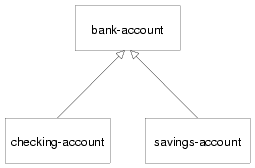
\includegraphics[scale=0.7]{images/account-hierarchy.png}
\end{figure}

Первой обобщённой функцией будет \lstinline{withdraw}, которая уменьшает баланс на указанную
сумму.  Если баланс меньше этой суммы, то она должна выдать ошибку и оставить баланс в
неизменном виде.  Вы можете начать с определения обобщённой функции при помощи
\lstinline{DEFGENERIC}.

Основная форма \lstinline{DEFGENERIC} похожа на \lstinline{DEFUN}, за тем исключением, что нет тела
функции.  Список параметров \lstinline{DEFGENERIC} определяет параметры, которые должны
приниматься всеми методами, определёнными для данной обобщённой функции.  Вместо тела
\lstinline{DEFGENERIC} может содержать различные опции.  Одной из опций, которую вы должны
всегда указывать, является \lstinline{:documentation}, которая используется для указания строки
с описанием назначения обобщённой функции.  Поскольку обобщённая функция является
полностью абстрактной, важно, чтобы и пользователь, и программист имели чёткое
представление о том, что она делает.  Таким образом, вы можете определить \lstinline{withdraw}
следующим образом:

\begin{myverb}
(defgeneric withdraw (account amount)
  (:documentation "Withdraw the specified amount from the account.
Signal an error if the current balance is less than amount."))
\end{myverb}

\section{DEFMETHOD}

Сейчас вы готовы к использованию \lstinline{DEFMETHOD} для определения методов, которые
реализуют \lstinline{withdraw}\footnote{С технической точки зрения, вы можете вообще не
  использовать \lstinline{DEFGENERIC}~-- если вы определяете метод с помощью \lstinline{DEFMETHOD} и
  соответствующая обобщённая функция не определена, она будет создана автоматически.
  Однако хорошим тоном считается явное определение обобщённой функции, поскольку это
  предоставляет хорошее место для документирования её предназначения.}\hspace{\footnotenegspace}.

Список параметров метода должен быть конгруэнтен его обобщённой функции.  В~данном случае
это означает, что все методы, определённые для \lstinline{withdraw}, должны иметь два
обязательных параметра.  В~более общих чертах методы должны иметь то же самое количество
обязательных и необязательных параметров и, кроме этого, должны уметь принимать любые
аргументы, относящиеся к остаточным (\lstinline!&rest!) или именованным (\lstinline!&key!)
параметрам, определённым в обобщённой функции\footnote{Метод может <<принимать>>
  именованные и остаточные аргументы, определённые в обобщённой функции, путём указания
  параметра \lstinline!&rest!, таких же именованных параметров или указания
  \lstinline!&allow-other-keys! вместе с \lstinline!&key!.  Метод также может указывать
  именованные параметры, не указанные в списке параметров обобщённой функции: когда
  вызывается обобщённая функция, будет принят любой именованный параметр, указанный
  обобщённой функцией или любым другим подходящим методом.  \textit{Одним следствием
    из правила соответствия является то, что все методы одной и той же обобщённой функции
    будут иметь совпадающие списки параметров.  Common Lisp не поддерживает перегрузку
    методов так, как это делают некоторые статически типизированные языки, как С++ и Java,
    где одно и то же имя может использоваться для методов с разными списками параметров.}}\hspace{\footnotenegspace}.

Поскольку базовые действия по списанию денег со счёта являются одинаковыми для всех
счетов, то вы можете определить метод, который специализирует параметр \lstinline{account}
для класса \lstinline{bank-account}.  Вы можете предположить, что функция
\lstinline{balance} возвращает текущее значение суммы на счёте и может быть использована
вместе с функцией \lstinline{SETF} (и~таким образом вместе с \lstinline{DECF}) для
установки значения баланса.  Функция \lstinline{ERROR} является стандартной функцией для
сообщения об ошибках, и я её подробно опишу в главе~\ref{ch:19}.  Используя эти две
функции, вы можете определить основной метод \lstinline{withdraw} примерно так:

\begin{myverb}
(defmethod withdraw ((account bank-account) amount)
  (when (< (balance account) amount)
    (error "Account overdrawn."))
  (decf (balance account) amount))
\end{myverb}

Как видно из этого кода, форма \lstinline{DEFMETHOD} более похожа на \lstinline{DEFUN}, по сравнению
с \lstinline{DEFGENERIC}.  Основным отличием является то, что требуемые параметры могут быть
специализированы путём замены имени параметра на список из двух элементов.  Первым
элементом является имя параметра, а вторым~-- специализатор, который может быть либо
именем класса, либо \lstinline{EQL}-специализатором, форму которого я опишу чуть позже.  Имя
параметра может быть любым~-- оно не обязательно должно совпадать с именем, указанным в
объявлении обобщённой функции, несмотря на то что чаще всего они совпадают.

Этот метод будет использоваться тогда, когда первый аргумент \lstinline{withdraw} является
экземпляром класса \lstinline{bank-account}.  Второй параметр, \lstinline{amount}, неявно
специализируется для класса \lstinline{T}, а поскольку все объекты являются экземплярами
\lstinline{T}, это никак не затрагивает применимость метода.

Теперь предположим, что все чековые счета имеют защиту от перерасхода.  Так что каждый
чековый счёт связан с другим счётом в банке, с которого будет производиться списание,
когда на чековом счету недостаточно денег для списания.  Вы можете предположить, что
функция \lstinline{overdraft-account} получает объект класса \lstinline{checking-account} и
возвращает объект класса \lstinline{bank-account}, представляющего собой связанный счёт.

Таким образом, списание с объекта класса \lstinline{checking-account} требует выполнения
дополнительных шагов в сравнении со списанием с обычного объекта \lstinline{bank-account}.
Сначала вы должны проверить, является ли списываемая сумма большей, чем имеющаяся на
счету, и если это так, то перенести недостающую сумму со связанного счёта.  Затем вы
можете продолжать так же, как и с обычным объектом \lstinline{bank-account}.

Так что вы можете захотеть определить метод \lstinline{withdraw}, специализированный для
\lstinline{checking-account}, для обработки перевода денег с другого счёта и последующей
передачи управления методу, специализированному для \lstinline{bank-account}.  Такой метод
может выглядеть вот так:

\begin{myverb}
(defmethod withdraw ((account checking-account) amount)
  (let ((overdraft (- amount (balance account))))
    (when (plusp overdraft)
      (withdraw (overdraft-account account) overdraft)
      (incf (balance account) overdraft)))
  (call-next-method))
\end{myverb}

Функция \lstinline{CALL-NEXT-METHOD} является частью системы обобщённых функций и используется
для комбинации \textit{подходящих} методов.  Она сообщает, что контроль должен быть
передан от текущего метода к методу, специализированному для
\lstinline{bank-account}\footnote{\lstinline{CALL-NEXT-METHOD} аналогичен вызову метода для
  \lstinline{super} в Java или использованию явно указанного метода или функции класса в Python
  или C++.}\hspace{\footnotenegspace}.  Когда он вызывается без аргументов, как это было сделано в нашем примере,
следующий в цепочке метод будет вызван с теми же аргументами, которые были переданы
обобщённой функции.  Он также может быть вызван с явным указанием аргументов, которые
будут переданы следующему методу.

Вам не обязательно вызывать \lstinline{CALL-NEXT-METHOD} в каждом методе.  Однако если вы не
будете вызывать эту функцию, то новый метод будет полностью отвечать за реализацию
требуемого поведения обобщённой функции.  Например, если вы хотите создать подкласс
\lstinline{bank-account}, названный \lstinline{proxy-account}, который не будет отслеживать свой
баланс, а вместо этого будет делегировать списание средств другому счёту, то вы можете
записать этот метод следующим образом (предполагая, что функция \lstinline{proxied-account}
возвращает соответствующий счёт):

\begin{myverb}
(defmethod withdraw ((proxy proxy-account) amount)
  (withdraw (proxied-account proxy) amount))
\end{myverb}

В~заключение \lstinline{DEFMETHOD} также позволяет вам создавать методы, которые
специализированы для конкретного объектаk используя \lstinline{EQL}-специализатор.  Например,
предположим, что банковское приложение \textit{будет} развёрнуто в каком-то
коррумпированном банке.  Предположим, что переменная \lstinline{*account-of-bank-president*}
хранит ссылку на конкретный банковский счёт, который относится (как это видно из имени) к
президенту банка.  Также предположим, что переменная \lstinline{*bank*} представляет весь банк,
а функция \lstinline{embezzle} крадёт деньги у банка.  Президент банка может попросить вас
<<исправить>> функцию \lstinline{withdraw} таким образом, чтобы она обрабатывала его счёт
другим способом.

\begin{myverb}
(defmethod withdraw ((account (eql *account-of-bank-president*)) amount)
  (let ((overdraft (- amount (balance account))))
    (when (plusp overdraft)
      (incf (balance account) (embezzle *bank* overdraft)))
  (call-next-method)))
\end{myverb}

Однако заметьте, что форма, указанная в \lstinline{EQL}-специализаторе, который используется
для указания объекта (в нашем случае это \lstinline{*account-of-bank-president*}), вычисляется
один раз, когда вычисляется \lstinline{DEFMETHOD}.  Этот метод будет специализирован для
значения \lstinline{*account-of-bank-president*} в тот момент, когда этот метод был определён;
последующие изменения переменной не изменяют метода.

\section{Комбинирование методов}

Вне кода метода использование \lstinline{CALL-NEXT-METHOD} не имеет смысла.  Внутри метода
использование этой функции обретает смысл за счёт того, что механизмы реализации
обобщённых функций при каждом запуске создают эффективный метод из методов, для которых
применимы текущие параметры.  Идея построения эффективного метода путём комбинации
методов, для которых применимы текущие аргументы, является основой концепции обобщённых
функций, и это позволяет обобщённым функциям реа\-ли\-зо\-вы\-вать возможности, которые недоступны
в системах с передачей сообщений.  Так что следует поближе познакомиться с тем, что в
действительности происходит.  Люди, которые давно знакомы с концепциями систем с передачей
сообщений, должны обратить на данный материал особое внимание, поскольку обобщённые функции
кардинально меняют диспатчеризацию методов, по сравнению с передачей сообщений, делая
обобщённую функцию (а не класс) ответственной за передачу управления.

В~соответствии с концепцией эффективный метод строится в три шага: на первом шаге
обобщённая функция строит список методов, для которых применимы переданные аргументы.  На
втором шаге полученный список методов сортируется в соответствии со специализированными
параметрами.  И в заключение методы по порядку берутся из списка, и их код комбинируется,
образуя эффективный метод\pclfootnote{Хотя построение эффективного метода кажется медленным,
  был достигнут достаточный прогресс в части обеспечения его эффективности и разработки
  быстрых реализаций Common Lisp.  Одной из стратегий является кэширование эффективных
  методов, так что следующие вызовы с теми же аргументами будут обрабатываться сразу.}.

Для нахождения методов, для которых применимы данные аргументы, обобщённая функция
сравнивает аргументы с соответствующими специализаторами параметров всех определённых
методов.  Метод считается допустимым, только если все специализаторы совместимы с
соответствующими параметрами.

Когда специализатор является именем класса, он считается совместимым, если указанное имя
совпадает с именем класса аргумента (или именем одного из суперклассов аргумента).
(Заметьте, что параметры без явных специализаторов неявно специализируются классом
\lstinline{T}, так что они будут совместимы с любым аргументом.)  \lstinline{EQL}-специализатор
считается совместимым, если аргумент является тем же объектом, что указан в
специализаторе.

Поскольку все аргументы проверяются относительно соответствующих специализаторов, все они
влияют на результаты выбора подходящих методов.  Методы, которые явно специализируют более
одного параметра, называются мультиметодами; я опишу их в разделе <<Мультиметоды>>.

После того как все соответствующие методы найдены, необходимо отсортировать их, чтобы
затем скомбинировать в эффективный метод.  Для упорядочения двух методов обобщённая
функция сравнивает их специализаторы параметров слева направо\footnote{В
  действительности порядок сравнения специализаторов настраивается через опцию
  \lstinline{:argument-precedence-order} макроса \lstinline{DEFGENERIC}, хотя она редко
  используется.}\hspace{\footnotenegspace}, и первый специализатор, который отличается в списке параметров методов,
будет определять их порядок, где первым ставится метод с более специфичным
специализатором.

Поскольку сортируются только подходящие методы, вы знаете все классы специализаторов, для
которых соответствующий аргумент является экземпляром.  В~типичном случае если два
специализатора класса отличаются, то один будет подклассом другого.  В~этом случае
специализатор, именующий подкласс, считается более специфичным.  Поэтому метод, который
специализирован для счёта с классом \lstinline{checking-account}, будет рассматриваться как
более специфичный, чем метод, специализированный для класса \lstinline{bank-account}.

Множественное наследование немного усложняет идею специфичности, поскольку аргумент может
быть экземпляром двух классов, ни один из которых не является подклассом другого.  Если
такие классы используются как специализаторы параметров, то обобщённая функция не может
упорядочить их, используя только правило, что подклассы являются более специфичными, чем их
суперклассы.  В~следующей главе я опишу, как понятие специфичности было расширено для
обработки множественного наследования.  Сейчас достаточно сказать, что существует алгоритм
для упорядочения специализаторов классов.

В~заключение надо отметить, что \lstinline{EQL}-специализатор всегда более специфичен, чем
любой специализатор класса, и поскольку рассматриваются только подходящие методы, то если
\lstinline{EQL}-специализатор конкретного параметра имеет более одного метода, то все они
должны иметь одинаковые \lstinline{EQL}-специализаторы.  Сравнение данных методов происходит на
основе других параметров.

\vfill{}

\section{Стандартный комбинатор методов}

Теперь, когда вы понимаете, как подходящие методы находятся и сортируются, вы готовы
поближе взглянуть на последний шаг~-- как отсортированный список методов комбинируется в
один эффективный метод.  По умолчанию обобщённые функции используют так называемый
<<стандартный комбинатор методов>>.  Стандартный комбинатор объединяет методы таким образом,
что \lstinline{CALL-NEXT-METHOD} работает, как это вы уже увидели: сначала запускается
наиболее специфичный метод, и каждый метод может передать управление следующему методу,
используя \lstinline{CALL-NEXT-METHOD}.

Однако тут есть больше возможностей.  Методы, которые я обсуждал, называются основными
методами.  Основные методы (как и предполагает их имя) отвечают за реализацию основной
функциональности обобщённых функций.  Стандартный комбинатор методов также поддерживает
три вида вспомогательных методов: \lstinline{:before}, \lstinline{:after} и \lstinline{:around}.
Определение вспомогательных методов записывается с помощью \lstinline{DEFMETHOD}, так же как и
для основных методов, но, кроме этого, между именем метода и списком параметров указывается
квалификатор метода, который именует тип метода.  Например, метод \lstinline{:before} для
функции \lstinline{withdraw}, которые специализирует параметр \lstinline{account} для класса
\lstinline{bank-account}, будет начинаться со следующей строки:

\begin{myverb}
(defmethod withdraw :before ((account bank-account) amount) ...)
\end{myverb}

Каждый вид вспомогательных методов комбинируется в эффективный метод разными способами.
Все применимые методы \lstinline{:before} (не только наиболее специфические) запускаются как
часть эффективного метода.  Они запускаются (как и предполагается их именем) до наиболее
специфического основного метода и запускаются, начиная с самого специфического метода.
Таким образом, методы \lstinline{:before} могут быть использованы для выполнения любой
подготовительной работы, которая может понадобиться, чтобы убедиться, что основной метод
может быть выполнен.  Например, вы можете использовать метод \lstinline{:before},
специализированный для \lstinline{checking-account}, для реализации защиты от перерасхода для
чековых счетов:

\begin{myverb}
(defmethod withdraw :before ((account checking-account) amount)
  (let ((overdraft (- amount (balance account))))
    (when (plusp overdraft)
      (withdraw (overdraft-account account) overdraft)
      (incf (balance account) overdraft))))
\end{myverb}

Этот метод \lstinline{:before} имеет три преимущества, по сравнению с использованием основного
метода.  Во-первых, он явно показывает, как метод изменяет общее поведение функции
\lstinline{withdraw},~-- он не пересекается с основным поведением и не изменяет возвращаемое
значение.

Следующим преимуществом является то, что главный метод, специализированный для класса,
более специфичного, чем \lstinline{checking-account}, не будет противоречить этому методу
\lstinline{:before}, что позволяет автору подкласса \lstinline{checking-account} более легко
расширить поведение \lstinline{withdraw}, при этом сохраняя старую функциональность.

И наконец, поскольку метод \lstinline{:before} не должен вызывать \lstinline{CALL-NEXT-METHOD} для
передачи управления оставшимся методам, нет возможности сделать ошибку, забыв указать эту
функцию.

Другие вспомогательные методы также организуются в эффективные методы способами, которые
отражены в их именах.  Все методы \lstinline{:after} запускаются после основного метода в
порядке, когда наиболее специфичный метод вызывается последним (порядок противоположен
вызову методов \lstinline{:before}).  Таким образом, методы \lstinline{:before} и \lstinline{:after}
комбинируются для создания вложенных обвязок вокруг основной функциональности,
обеспечиваемой основными методами,~-- каждый более специфичный метод \lstinline{:before} получит
шанс сделать что-то для менее специфичного метода \lstinline{:before}, основные методы могут
успешно выполняться, и затем каждый более специфичный метод \lstinline{:after} получает шанс
убрать что-то за основным методом и менее специфичными методами \lstinline{:after}.

И наконец, методы \lstinline{:around} комбинируются практически, также как и основные
методы, за исключением того, что они выполняются <<вокруг>> остальных методов. Так что код
наиболее специфического метода \lstinline{:around} запускается до любого кода. Внутри кода
метода \lstinline{:around} вызов \lstinline{CALL-NEXT-METHOD} приведёт к тому, что будет
выполняться код сле\-дую\-ще\-го метода \lstinline{:around}, или, при вызове из наименее
специфического метода \lstinline{:around}, приведёт к выполнению цепочки методов
\lstinline{:before}, основного метода и затем методов \lstinline{:after}.  Почти все
методы \lstinline{:around} будут иметь в своём коде вызов \lstinline{CALL-NEXT-METHOD},
поскольку метод \lstinline{:around} без такого вызова не будет полностью перехватывать
обобщённую функцию и все её методы, за исключением более специфичных методов
\lstinline{:around}.

Иногда требуется полный перехват действий, но обычно методы \lstinline{:around} используются
для установки некоторого динамического контекста, в котором будут выполняться остальные
методы,~-- например, для связывания динамической переменной или для установки обработчика
ошибок (это я буду обсуждать в главе~\ref{ch:19}).  Метод \lstinline{:around} может не вызывать
\lstinline{CALL-NEXT-METHOD} в тех случаях, если он, например, возвращает кэшированое значение,
которое было получено при предыдущих вызовах \lstinline{CALL-NEXT-METHOD}.  В~любом случае,
метод \lstinline{:around}, не вызывающий \lstinline{CALL-NEXT-METHOD}, ответствен за корректную
реа\-ли\-за\-цию семантики обобщённой функции для всех классов аргументов, для которых этот
метод может применяться, включая и будущие подклассы.

Вспомогательные методы являются лишь удобным и лаконичным способом для выражения некоторых
общих подходов (шаблонов).  Они не позволяют сделать ничего невозможного посредством
объединения основных методов с аккуратным соблюдением нескольких соглашений по кодированию
и небольшим количеством дополнительного кода. Вероятно, наибольшей выгодой является то,
что они обеспечивают унифицированный каркас для расширения функциональности обобщённых
функций.  Библиотеки часто определяют обобщённые функции и основные методы для них,
позволяя пользователям изменять их поведение с помощью вспомогательных методов.

\section{Другие комбинаторы методов}

В~добавление к стандартному комбинатору методов язык реализует девять других встроенных
комбинаторов методов, известных как <<простые встроенные комбинаторы методов>>.  Вы также
можете определить собственный комбинатор методов, хотя это довольно редко используемая
возможность, описание которой не является предметом этой книги.  Я коротко опишу, как
использовать простые комбинаторы методов, чтобы дать общее представление об имеющихся
возможностях.

Все простые комбинаторы используют одинаковую стратегию: вместо запуска наиболее
специфического метода и разрешения ему запускать менее специфичные методы через
\lstinline{CALL-NEXT-METHOD} простые комбинаторы методов создают эффективный метод, содержащий
код всех основных методов, расположенных по порядку и обернутых вызовом к функции,
макросу или специальному оператору, который и дал комбинатору методов соответствующее имя.
Девять комбинаторов получили имена от операторов: \lstinline{+}, \lstinline{AND}, \lstinline{OR},
\lstinline{LIST}, \lstinline{APPEND}, \lstinline{NCONC}, \lstinline{MIN}, \lstinline{MAX} и \lstinline{PROGN}.  Простые
комбинаторы поддерживают только два типа методов~-- основные методы, которые объединяются
так, как было описано выше, и методы \lstinline{:around}, которые работают так же, как и методы
\lstinline{:around} в стандартном комбинаторе.

Например, обобщённая функция, которая использует комбинатор методов \lstinline{+}, вернёт сумму
всех результатов, возвращённых вызванными основными методами.  Отметьте, что комбинаторы
\lstinline{AND} и \lstinline{OR} не обязательно будут выполнять все основные методы, поскольку эти
макросы могут использовать сокращённую схему работы,~-- обобщённая функция, использующая
комбинатор \lstinline{AND}, вернёт значение \lstinline{NIL} сразу же, как один из методов вернёт его,
или в противном вернёт значение, возвращённое последним вызванным методом.  Аналогичным
образом комбинатор \lstinline{OR} вернёт первое значение, не равное-\lstinline{NIL}, возвращённое
любым из его методов.

Для определения обобщённой функции, которая использует конкретный комбинатор методов, вы
должны указать опцию \lstinline{:method-combination} при объявлении \lstinline{DEFGENERIC}.
Значение, указанное данной опцией, определяет имя комбинатора методов, который вы хотите
использовать.  Например, для определения обобщённой функции \lstinline{priority}, которая
возвращает сумму значений, возвращаемых отдельными методами, используя комбинатор методов
\lstinline{+}, вы можете написать следующий код:

\begin{myverb}
(defgeneric priority (job)
  (:documentation "Return the priority at which the job should be run.")
  (:method-combination +))
\end{myverb}

По умолчанию все эти комбинаторы методов комбинируют методы в порядке, начиная с наиболее
специфичного.  Однако вы можете изменить порядок путём указания ключевого слова
\lstinline{:most-specific-last} после имени комбинатора в объявлении функции с помощью
\lstinline{DEFGENERIC}.  Порядок, скорее всего, не имеет значения, если вы используете комбинатор
\lstinline{+} и методы не имеют побочных эффектов, но в целях демонстрации я изменю код
\lstinline{priority}, чтобы он использовал порядок \lstinline{most-specific-last}:

\begin{myverb}
(defgeneric priority (job)
  (:documentation "Return the priority at which the job should be run.")
  (:method-combination + :most-specific-last))
\end{myverb}

Основные методы обобщённых функций, которые используют один из этих комбинаторов, должны
быть квалифицированы именем комбинатора методов.  Таким образом, основной метод,
определённый для функции \lstinline{priority}, может выглядеть следующим образом:

\begin{myverb}
(defmethod priority + ((job express-job)) 10)
\end{myverb}

Это станет более ясным, если вы рассмотрите определение метода как конкретную часть
обобщённой функции.

Все простые встроенные комбинаторы методов поддерживают методы \lstinline{:around}, которые
работают так же, как и методы \lstinline{:around} в стандартном комбинаторе: наиболее специфичный
метод \lstinline{:around} выполняется до любого метода, и он может использовать
\lstinline{CALL-NEXT-METHOD} для передачи контроля менее специфичному методу \lstinline{:around} до
тех пор, пока не будет достигнут основной метод.  Опция \lstinline{:most-specific-last} не
влияет на порядок вызова методов \lstinline{:around}.  И, как я отметил ранее, встроенные
комбинаторы методов не поддерживают методов \lstinline{:before} и \lstinline{:after}.

Подобно стандартному комбинатору методов, эти комбинаторы не позволяют вам сделать ничего
из того, что вы не можете сделать <<вручную>>.  Вместо этого они позволяют вам выразить то,
что вы хотите, а язык возьмёт на себя заботу о связывании всего вместе, делая ваш код
более кратким и выразительным.

Честно говоря, примерно в 99 процентах случаев вам будет достаточно стандартного
комбинатора методов.  Оставшийся один процент случаев, скорее всего, будет обработан
простыми встроенными комбинаторами методов.  Но если вы попадёте в ситуацию
(вероятность~-- примерно одна сотая процента), когда вам не будет подходить ни один из
встроенных комбинаторов, то вы можете посмотреть на описание
\lstinline{DEFINE-METHOD-COMBINATION} в вашем любимом справочнике по Common Lisp.

\section{Мультиметоды}

Методы, которые явно специализируют более одного параметра обобщённой функции, называются
\textit{мультиметодами}.  Мультиметоды~-- это то, в чем реально расходятся обобщённые
функции и передача сообщений.  Языки с передачей сообщений не приспособлены к
мультиметодам, поскольку они не относятся к конкретному классу; вмес\-то этого каждый
мультиметод определяет часть реализации конкретной обобщённой функции, которая применяется
тогда, когда эта функция вызывается с аргументами, которые соответствуют всем
специализированным параметрам.

Мультиметоды полезны в ситуациях, когда вы не знаете, к какому классу определённое
поведение должно относиться (в языках с передачей сообщений).  Звук, который издаёт
барабан, когда вы стучите по нему палочкой, является функцией барабана или функцией
палочки?  Конечно, он принадлежит обоим предметам.  Для моделирования такой ситуации в
Common Lisp вы просто определяете функцию \lstinline{beat}, которая принимает два аргумента.

Затем вы можете определять разные мультиметоды для реализации \lstinline{beat} для комбинаций,
которые вам нужны. Например:

\begin{myverb}
(defmethod beat ((drum snare-drum) (stick wooden-drumstick)) ...)
(defmethod beat ((drum snare-drum) (stick brush)) ...)
(defmethod beat ((drum snare-drum) (stick soft-mallet)) ...)
(defmethod beat ((drum tom-tom) (stick wooden-drumstick)) ...)
(defmethod beat ((drum tom-tom) (stick brush)) ...)
(defmethod beat ((drum tom-tom) (stick soft-mallet)) ...)
\end{myverb}

Мультиметоды не помогают от комбинаторного взрыва~-- если вам необходимо смоделировать
пять видов барабанов и шесть видов палочек и каждая из комбинаций даёт отдельный звук, то
нет способа упростить это; вам необходимо определить тридцать различных методов для
реализации всех комбинаций, используя мультиметоды или нет.  Мультиметоды помогут вам не
писать собственный код для диспатчинга, позволяя использовать встроенные средства
диспатчеризации, которые были очень удобны при работе с методами, специализированными для
одного параметра\pclfootnote{В~языках без мультиметодов вы должны сами писать
  диспатчеризующий код для реализации поведения, которое зависит от нескольких объектов.
  Назначением популярного паттерна проектирования <<Визитор (Visitor)>> является
  упорядочение серии методов, диспатчеризуемых по одному классу, таким образом, чтобы они
  обеспечивали множественную диспатчеризацию.  Однако это требует, чтобы один набор
  классов знал о других.  Паттерн <<Визитор>> также вязнет в комбинаторном росте
  дис\-пат\-че\-ри\-зуе\-мых методов, если он используется для диспатчеризации более чем двух
  объектов.}.

\begin{lrbox}{\chonesixone}
  \begin{minipage}{\linewidth}
\begin{myverb}
public class A {
  public void foo(A a) { System.out.println("A/A"); }
  public void foo(B b) { System.out.println("A/B"); }
}

public class B extends A {
  public void foo(A a) { System.out.println("B/A"); }
  public void foo(B b) { System.out.println("B/B"); }
}
\end{myverb}
  \end{minipage}
\end{lrbox}

\begin{lrbox}{\chonesixtwo}
  \begin{minipage}{\linewidth}
\begin{myverb}
public class Main {
  public static void main(String[] argv) {
    A obj = argv[0].equals("A") ? new A() : new B();
    obj.foo(obj);
  }
}
\end{myverb}
  \end{minipage}
\end{lrbox}

\begin{lrbox}{\chonesixthree}
  \begin{minipage}{\linewidth}
\begin{myverb}
bash\$ java com.gigamonkeys.Main A
A/A
\end{myverb}
  \end{minipage}
\end{lrbox}

\begin{lrbox}{\chonesixfour}
  \begin{minipage}{\linewidth}
\begin{myverb}
bash\$ java com.gigamonkeys.Main B
B/A
\end{myverb}
  \end{minipage}
\end{lrbox}

\begin{myverb}
(defgeneric beat (drum stick)
  (:documentation
   "Produce a sound by hitting the given drum with the given stick."))
\end{myverb}

\textintable{Мультиметоды против перегрузки методов}{Программисты, использовавшие статически типизованные языки с системами передачи сообщений,
такие как Java и C++, могут подумать, что мультиметоды похожи на такую возможность этих
языков, как перегрузка методов.  Однако эти две возможности языка в достаточной мере
отличаются, поскольку перегруженные методы выбираются во время компиляции, основываясь на
информации об аргументах, полученной во время компиляции, а не во время исполнения.  Чтобы
посмотреть, как это работает, рассмотрим два следующих класса на языке Java:\\[-3pt]

\noindent{}\usebox{\chonesixone}\\

Теперь посмотрим, что случится, когда вы запустите метод \lstinline{main} из этого класса.\\[-3pt]

\noindent{}\usebox{\chonesixtwo}\\

Когда вы заставляете \lstinline{main} создать экземпляр \lstinline{A}, она выдаст \lstinline{A/A}, как вы и
ожидали.\\[-3pt]

\noindent{}\usebox{\chonesixthree}\\

Однако если вы заставите \lstinline{main} создать экземпляр \lstinline{B}, то настоящий тип объекта
\lstinline{obj} будет принят во внимание не полностью.\\[-3pt]

\noindent{}\usebox{\chonesixfour}\\

Если бы перегруженные методы работали так же, как и мультиметоды в Common Lisp, то программа
бы выдала ожидаемый результат: \lstinline{B/B}.  Существует возможность реа\-ли\-за\-ции
множественной диспатчеризации для систем с передачей сообщений вручную, но это будет
противоречить модели системы с передачей сообщений, поскольку метод с множественной
диспатчеризацией не должен относиться ни к одному из классов.}

Мультиметоды также спасают вас от требования, чтобы один набор классов был тесно связан с
другим набором. В~нашем примере барабанов/палочек не требуется, чтобы класс,
представляющий барабаны, знал о различных классах, представляющих барабанные палочки, и
наоборот.  Мультиметоды связывают независимые классы для описания их совместного
поведения, при этом не требуя никакого взаимодействия между самими классами.

\section{Продолжение следует...}

Я описал основы (и немного больше) обобщённых функций~-- <<глаголов>> объектной системы
Common Lisp.  В~следующей главе я покажу вам, как определять ваши собственные классы.

%%% Local Variables: 
%%% mode: latex
%%% TeX-master: "pcl-ru"
%%% TeX-open-quote: "<<"
%%% TeX-close-quote: ">>"
%%% End: 


\chapter{Переходим к объектам: Классы}
\label{ch:17}

Если обобщённые функции являются глаголами объектной системы, то классы являются
существительными.  Как я упоминал в предыдущей главе, все значения в программах на Common
Lisp являются экземплярами какого-то из классов.  Более того, все классы образуют иерархию
на вершине которой находится класс \code{T}.

Иерархия классов состоит из двух основных семейств классов: встроенных и определённых
пользователем.  Классы, которые представляют типы данных, которые мы изучали до сих
пор~--- такие как \code{INTEGER}, \code{STRING} и \code{LIST}, являются встроенными.  Они
находятся в отдельном разделе иерархии классов, организованные соответствующими связями
дочерних и родительских классов, и для работы с ними используются функции, которые я
описывал на протяжении всей книги.  Вы не можете унаследовать от этих классов, но как вы
увидели в предыдущем разделе, вы можете определить специализированные методы для них,
эффективно расширяя поведения этих классов.\footnote{Определение новых методов для
    существующих классов может показаться странным для людей, которые использовали
    статически типизированные языки, такие как C++ и Java, в которых все методы классов
    должны быть определены как часть определения класса.  А вот программисты, которые
    имеют опыт программирования на Smalltalk и Objective C не найдут в этой
функциональности ничего странного.}

Но когда вы создаёте новые существительные~--- например, классы, которые использовались в
предыдущей главе для представления банковских счетов, то вам нужно определить ваши
собственные классы.  Это и будет темой данной главы.

\section{DEFCLASS}

Вы можете создать собственный класс с помощью макроса \code{DEFCLASS}.  Поскольку
поведение класса определяется обобщёнными функциями, и методами, специализированными для
класса, то \code{DEFCLASS} отвечает только за определение класса как типа данных.

Класс, как тип данных, состоит из трёх частей: имени, отношения к другим классам и имен
слотов.\footnote{В других объектно-ориентированных языках слоты могут называться полями,
переменными-членами класса или аттрибутами.}  Базовая форма \code{DEFCLASS} выглядит
достаточно просто.

\begin{lstlisting}
(defclass name (direct-superclass-name*)
  (slot-specifier*))
\end{lstlisting}

Что такое классы, определённые пользователем?

<<Определённые пользователем классы>>~--- термин не из стандарта языка. Определёнными
пользователем классами я называю подклассы класса \code{STANDARD-OBJECT}, а также классы,
у которых метакласс~--- \code{STANDARD-CLASS}. Но поскольку я не собираюсь говорить о
способах определения классов, которые не наследуют \code{STANDARD-OBJECT} и чей метакласс
~--- это не \code{STANDARD-CLASS}, вам можно не обращать на это внимания. Определённые
пользователем~--- не идеальный термин, потому что реализация может определять некоторые
классы таким же способом. Но ещё большей путаницей будет называть эти классы стандартными,
поскольку встроенные классы (например, \code{INTEGER} и \code{STRING}) тоже стандартные,
если не сказать больше, потому что они определены стандартом языка, но они не расширяют
(не наследуют) \code{STANDARD-OBJECT}. Чтобы ещё больше запутать дело, пользователь может
также определять классы, не наследующие \code{STANDARD-OBJECT}. В частности, макрос
\code{DEFSTRUCT} тоже определяет новые классы. Но это во многом для обратной совместимости
~--- \code{DEFSTRUCT} появился раньше, чем CLOS и был изменён, чтоб определять классы, когда
CLOS добавлялся в язык. Но создаваемые им классы достаточно ограничены по сравнению с
классами, созданными с помощью \code{DEFCLASS}. Итак, я буду обсуждать только классы,
создаваемые с помощью \code{DEFCLASS}, которые используют заданный по умолчанию метакласс
\code{STANDARD-CLASS} и, за неимением лучшего термина, назову их <<определёнными
пользователем классами>>.

Также как с функциями и переменными, вы можете использовать в качестве имени класса любой
символ.\footnote{Также, как и при именовании функции и переменных, это не совсем правда,
  что вы можете использовать для класса любое имя~--- вы не можете использовать имена,
  определённые стандартом.  В главе~\ref{ch:21} вы увидите как можно избежать таких конфликтов
  имён.}  Имена классов находятся в собственном пространстве имён, отдельно от имен
функций и переменных, так что вы можете задать для класса то же самое имя, что и
существующие функция и переменная.  Вы будете использовать имя класса в качестве аргумента
функции \code{MAKE-INSTANCE}, которая создаёт новые экземпляры классов, определённых
пользователем.

Опция \code{direct-superclass-names} используется для указания имён классов, от которых
будет проводиться наследование данного класса.  Если ни одного класса не указано, то он
будет унаследован от \code{STANDARD-OBJECT}.  Все классы, указанные в данной опции, должны
быть классами, определёнными пользователем, чтобы быть увереным, что каждый новый класс
происходит от \code{STANDARD-OBJECT}.  \code{STANDARD-OBJECT} является подклассом
\code{T}, так что все классы, определённые пользователем, являются частью одной иерархии
классов, которая также содержит все встроенные классы.

На время отвлекаясь от упоминания спецификаторов слотов, запись \code{DEFCLASS} для
некоторых из классов, которые мы использовали в предыдущей главе, может выглядеть
следующим образом:

\begin{lstlisting}
(defclass bank-account () ...)

(defclass checking-account (bank-account) ...)

(defclass savings-account (bank-account) ...)
\end{lstlisting}

В разделе~\ref{sec:17-multi-inheritance} я объясню, что означает указание более чем одного
суперкласса в списке опции \code{direct-superclass-names}.

\section{Спецификаторы слотов}

Большая часть \code{DEFCLASS} состоит из списка спецификаторов слотов.  Каждый
спецификатор определяет слот, который будет частью экземпляра класса.  Каждый слот в
экземпляре является местом, которое может хранить значение, к которому можно получить
доступ через функцию \code{SLOT-VALUE}. \code{SLOT-VALUE} в качестве аргументов принимает
объект и имя слота и возвращает значение нужного слота в данном объекте.  Эта функция
может использоваться вместе с \code{SETF} для установки значений слота в объекте.

Класс также наследует спецификаторы слотов от своих суперклассов, так что набор слотов,
присутствующих в любом объекте, является объединением всех слотов, указанных в форме
\code{DEFCLASS} для класса, а также указанных для всех его суперклассов.

По минимуму, спецификатор слота указывает его имя, так что спецификатор может быть простым
именем.  Например, вы можете определить класс \code{bank-account} с двумя слотами~---
\code{customer-name} и \code{balance}, например, вот так:

\begin{lstlisting}
(defclass bank-account ()
  (customer-name
   balance))
\end{lstlisting}

Каждый экземпляр этого класса содержит два слота: один для хранения имени клиента, а
второй ~--- для хранения текущего баланса счёта.  Используя данное определение вы можете
создать новые объекты \code{bank-account} с помощью \code{MAKE-INSTANCE}.

\begin{lstlisting}[style=lisprepl]
  (make-instance 'bank-account) ==> #<BANK-ACCOUNT @ #x724b93ba>
\end{lstlisting}

Аргументом \code{MAKE-INSTANCE} является имя класса, а возвращаемым значением~--- новый
объект.\footnote{В действительности, аргументом \code{MAKE-INSTANCE} может быть либо имя
  класса, или объект класса, возвращаемый функциями \code{CLASS-OF} или
  \code{FIND-CLASS}.}  Печатное представление объекта определяется обобщённой функцией
\code{PRINT-OBJECT}.  В этом случае, подходящим методом будет тот, который предоставляется
реализацией и специализированный для \code{STANDARD-OBJECT}.  Поскольку не каждый объект
может быть выведен таким образом, чтобы потом быть считанным назад, то метод печати для
\code{STANDARD-OBJECT} использует синтаксис \lstinline!#<>!, который заставит процедуру
чтения выдать ошибку, если он попытается прочитать его.  Оставшаяся часть представления
зависит от реализации, но обычно оно похоже на результат, приведённый выше, включая имя
класса и некоторое значение, например, адрес объекта в памяти.  В главе~\ref{ch:23} вы
увидите пример того, как определить метод для \code{PRINT-OBJECT} чтобы некоторые классы
можно было вывести в более информативной форме.

Используя данное определение \code{bank-account}, новые объекты будут создаваться со
слотами, которые не связаны со значениями.  Любая попытка получить значение для
несвязанного значения приведёт к выдаче ошибки, так что вы должны задать значение до того,
как вы будете считывать значения.

\begin{lstlisting}[style=lisprepl]
  (defparameter *account* (make-instance 'bank-account))  ==> *ACCOUNT*
  (setf (slot-value *account* 'customer-name) "John Doe") ==> "John Doe"
  (setf (slot-value *account* 'balance) 1000)             ==> 1000
\end{lstlisting}

Теперь вы можете получать значения слотов.

\begin{lstlisting}[style=lisprepl]
  (slot-value *account* 'customer-name) ==> "John Doe"
  (slot-value *account* 'balance)       ==> 1000
\end{lstlisting}

\section{Инициализация объекта}

Поскольку мы мало что можем сделать с объектом, который имеет пустые слоты, было бы хорошо
иметь возможность создавать объекты с инициализированными слотами.  Common Lisp
предоставляет три способа управления начальными значениями слотов.  Первые два требуют
добавления опций в спецификаторы слотов в \code{DEFCLASS}: с помощью опции \code{:initarg}
вы можете указать имя, которое потом будет использоваться как именованный параметр при
вызове \code{MAKE-INSTANCE} и переданное значение будет сохранено в слоте.  Вторая опция
~--- \code{:initform}, позволяет вам указать выражение на Lisp, которое будет использоваться
для вычисления значения, если при вызове \code{MAKE-INSTANCE} не был передан аргумент
\code{:initarg} .  В заключение, для полного контроля за инициализацией объекта, вы можете
определить метод для обобщённой функции \code{INITIALIZE-INSTANCE}, которую вызывает
\code{MAKE-INSTANCE}.\footnote{Другим способом установки значений слотов, является
  использование опции \code{:default-initargs} при объявлении \code{DEFCLASS}.  Эта опция
  используется для указания выражений, которые будут вычислены для нахождения аргументов
  для отдельных параметров инициализации, которые не получили значение при вызове
  \code{MAKE-INSTANCE}.  В текущий момент времени вам не нужно беспокоиться о
  \code{:default-initargs}.}

Спецификатор слота, который включает опции, такие как \code{:initarg} или
\code{:initform}, записывается как список, начинающийся с имени слота, за которым следуют
опции.  Например, если вы измените определение \code{bank-account} таким образом, чтобы
позволить передавать имя клиента и начальный баланс при вызове \code{MAKE-INSTANCE}, а
также чтобы установить для баланса начальное значение равное нулю, вы должны написать:

\begin{lstlisting}
(defclass bank-account ()
  ((customer-name
    :initarg :customer-name)
   (balance
    :initarg :balance
    :initform 0)))
\end{lstlisting}

Теперь вы можете одновременно создавать счёт и указывать значения слотов.

\begin{lstlisting}
(defparameter *account*
  (make-instance 'bank-account :customer-name "John Doe" :balance 1000))

  (slot-value *account* 'customer-name) ==> "John Doe"
  (slot-value *account* 'balance)       ==> 1000
\end{lstlisting}

Если вы не передадите аргумент \code{:balance} при вызове \code{MAKE-INSTANCE}, то вызов
\code{SLOT-VALUE} для слота \code{balance} будет получен вычислением формы, указанной
опцией \code{:initform}.  Но, если вы не передадите аргумент \code{:customer-name}, то
слот \code{customer-name} будет пустой, и попытка считывания значения из него, приведёт к
выдаче ошибки.

\begin{lstlisting}[style=lisprepl]
  (slot-value (make-instance 'bank-account) 'balance)       ==> 0
  (slot-value (make-instance 'bank-account) 'customer-name) ==> Ошибка (error)
\end{lstlisting}

Если вы хотите убедиться, что имя клиента было задано при создании счёта, то вы можете
выдать ошибку в начальном выражении (\code{initform}), поскольку оно будет вычислено
только если начальное значение (\code{initarg}) не было задано.  Вы также можете
использовать начальные формы, которые создают разные значения при каждом запуске~---
начальное выражение вычисляется заново для каждого объекта.  Для эксперементирования с
этими возможностями, вы можете изменить спецификатор слота \code{customer-name} и добавить
новый слот, \code{account-number}, который инициализируется значением увеличивающегося
счётчика.

\begin{lstlisting}
(defvar *account-numbers* 0)

(defclass bank-account ()
  ((customer-name
    :initarg :customer-name
    :initform (error "Must supply a customer name."))
   (balance
    :initarg :balance
    :initform 0)
   (account-number
    :initform (incf *account-numbers*))))
\end{lstlisting}

В большинстве случаев, комбинации опций \code{:initarg} и \code{:initform} будет
достаточно для нормальной инициализации объекта.  Однако, хотя начальное выражение может
быть любым выражением Lisp, оно не имеет доступа к инициализируемому объекту, так что оно
не может инициализировать один слот, основываясь на значении другого.  Для выполнения
такой задачи вам необходимо определить метод для обобщённой функции
\code{INITIALIZE-INSTANCE}.

Основной метод \code{INITIALIZE-INSTANCE}, специализированный для \code{STANDARD-OBJECT}
берёт на себя заботу об инициализации слотов, основываясь на данных, заданных опциями
\code{:initarg} и \code{:initform}.  Поскольку вы не захотите вмешиваться в этот процесс,
то наиболее широко применяемым способом является определение метода \code{:after},
специализированного для вашего класса.\footnote{Добавление метода \code{:after} к
  \code{INITIALIZE-INSTANCE} является аналогом на Common Lisp определению конструктора в
  Java или C++, или методу \lstinline!__init__! в Python.}  Например, предположим, что вы
хотите добавить слот \code{account-type}, который должен быть установлен в значение
\code{:gold}, \code{:silver} или \code{:bronze}, основываясь на начальном балансе счёта.
Вы можете изменить определение класса на следующее, добавляя слот \code{account-type} без
каких либо опций:

\begin{lstlisting}
(defclass bank-account ()
  ((customer-name
    :initarg :customer-name
    :initform (error "Must supply a customer name."))
   (balance
    :initarg :balance
    :initform 0)
   (account-number
    :initform (incf *account-numbers*))
   account-type))
\end{lstlisting}

После этого вы можете определить метод \code{:after} для \code{INITIALIZE-INSTANCE},
который установит значение слота \code{account-type}, основываясь на значении, которое
было сохранено в слоте \code{balance}.\footnote{Одна из ошибок, которую вы могли сделать
  до того, как освоились со вспомогательными методами, является в определении метода для
  \code{INITIALIZE-INSTANCE}, но без квалификатора \code{:after}.  Если вы сделаете это,
  вы получите новый основной метод, который скроет метод, вызываемый по умолчанию.  Вы
  можете удалить ненужный основной метод с помощью функций \code{REMOVE-METHOD} и
  \code{FIND-METHOD}.  Некоторые среды разработки могут предоставлять графический
  интерфейс для выполнения данной задачи.

\begin{lstlisting}
(remove-method #'initialize-instance
  (find-method #'initialize-instance () (list (find-class 'bank-account)))
\end{lstlisting}
}

\begin{lstlisting}
(defmethod initialize-instance :after ((account bank-account) &key)
  (let ((balance (slot-value account 'balance)))
    (setf (slot-value account 'account-type)
          (cond
            ((>= balance 100000) :gold)
            ((>= balance 50000) :silver)
            (t :bronze)))))
\end{lstlisting}

Указание \lstinline!&key! в списке параметров требуется обязательно, чтобы сохранить
список параметров соответствующим списку параметров обобщённой функции~--- список
параметров, указанный для функции \code{INITIALIZE-INSTANCE} включает \lstinline!&key!
чтобы позволить отдельным методам передавать собственные именованные параметры, но при
этом, он не требует указания конкретных названий.  Таким образом, каждый метод должен
указывать \lstinline!&key!, даже если он не указывает ни одного именованного параметра.

С другой стороны, если метод \code{INITIALIZE-INSTANCE}, специализированный для
конкретного класса, указывает именованный параметр, то этот параметр становится допустимым
параметром для функции \code{MAKE-INSTANCE} при создании экземпляра данного класса.
Например, если банк иногда платит процент начального баланса в качестве премии при
открытии счёта, то вы можете реализовать эту функцию, используя метод
\code{INITIALIZE-INSTANCE}, который получает именованный аргумент, указывающий процент
премии, например вот так:

\begin{lstlisting}
(defmethod initialize-instance :after ((account bank-account)
                                       &key opening-bonus-percentage)
  (when opening-bonus-percentage
    (incf (slot-value account 'balance)
          (* (slot-value account 'balance) (/ opening-bonus-percentage 100)))))
\end{lstlisting}

Путём определения метода \code{INITIALIZE-INSTANCE}, вы делаете
\code{:opening-bonus-percentage} допустимым аргументом функции \code{MAKE-INSTANCE} при
создании объекта \code{bank-account}.

\begin{lstlisting}[style=lisprepl]
  CL-USER> (defparameter *acct* (make-instance
                                  'bank-account
                                   :customer-name "Sally Sue"
                                   :balance 1000
                                   :opening-bonus-percentage 5))
  *ACCT*
  CL-USER> (slot-value *acct* 'balance)
  1050
\end{lstlisting}

\section{Функции доступа}

\code{MAKE-INSTANCE} и \code{SLOT-VALUE} дают вам возможности для создания и работы с
экземплярами ваших классов.  Все остальные операции могут быть реализованы в терминах этих
двух функций.  Однако, как знает всякий, знакомый с принципами правильного
объектно-ориентированного программирования, прямой доступ к слотам (полям или
переменным-членам) объекта может привести к получению уязвимого кода.  Проблема
заключается в том, что прямой доступ к слотам делает ваш код слишком связанным с
конкретной структурой классов.  Например, предположим, что вы решили изменить определение
\code{bank-account} таким образом, что вместо хранения текущего баланса в виде числа, вы
храните его в виде списка списаний и помещений денег на счёт, вместе с датами этих
операций.  Код, который имеет прямой доступ к слоту \code{balance} скорее всего будет
сломан, если вы измените определение класса, удалив слот или храня список в данном
слоте. С другой стороны, если вы определить функцию \code{balance}, которая осуществляет
доступ к слоту, то вы можете позже переопределить её, чтобы сохранить её поведение, даже
если изменится внутреннее представление данных.  И код, который использует такую функцию
будет продолжать нормально работать не требуя внесения изменений.

Другим преимуществом использования функций доступа вместо прямого доступа к слотам через
\code{SLOT-VALUE} является то, что их использование позволяет вам ограничить возможность
внешней модификации слота.\footnote{Конечно, предоставление функции доступа в
  действительности не ограничивает ничего, поскольку сторонний код все равно может
  использовать \code{SLOT-VALUE} для прямого доступа к слотам. Common Lisp не
  предоставляет строгой инкапсуляции слотов, как это делают C++ и Java; однако, если автор
  класса предоставляет функции доступа и вы игнорируете их, вместо этого используя
  \code{SLOT-VALUE}, то вы должны лучше знать, что вы делаете.  Кроме этого, имеется
  возможность использования пакетной системы, которую я буду обсуждать в
  главе~\ref{ch:21}, чтобы ограничить прямой доступ к некоторым слотам путём отсутствия
экспорта имён слотов.} Для пользователей класса \code{bank-account} может быть удобным
использование функций доступа для получения текущего баланса, но вы можете захотеть, чтобы
все изменения баланса производились через другие предоставляемые вами функции, такие как
\code{deposit} и \code{withdraw}.  Если клиент знает, что он сможет работать с объектами
только через определённый набор функций, то вы можете предоставить ему функцию
\code{balance}, но сделать так, чтобы для неё нельзя было выполнить \code{SETF}, чтобы
баланс был доступен только для чтения.

В заключение, использование функций доступа делает ваш код более аккуратным, поскольку вы
избегаете использования множества менее понятных функций \code{SLOT-VALUE}.

Определение функции, которая читает содержимое слота \code{balance} является тривиальным.

\begin{lstlisting}
(defun balance (account)
  (slot-value account 'balance))
\end{lstlisting}

Однако, если вы знаете, что вы будете определять подклассы для \code{bank-account}, то
может быть хорошей идеей определение \code{balance} в качестве обобщённой функции.  Таким
образом вы можете определить разные методы для \code{balance} для некоторых подклассов,
или расширить её возможности с помощью вспомогательных методов. Так что вместо предыдущего
примера можете написать следующее:

\begin{lstlisting}
(defgeneric balance (account))

(defmethod balance ((account bank-account))
  (slot-value account 'balance))
\end{lstlisting}

Как я только что обсуждал, вы не хотите, чтобы пользователь имел возможность устанавливать
баланс напрямую, но для других слотов, таких как \code{customer-name}, вы также можете
захотеть предоставить функцию для установки их значений.  Наиболее понятным способом будет
определение такой функции как \code{SETF}-функции.

\code{SETF}-функция является способом расширения функциональности \code{SETF}, определяя
новый вид места (place), для которого известно как устанавливать его значение.  Имя
\code{SETF}-функции является списком из двух элементов, где первый элемент является
символом \code{setf}, а второй~--- другим символом, обычно именем функции, которая
используется для доступа к месту, значение которого будет устанавливать функция
\code{SETF}.  \code{SETF}-функция может получать любое количество аргументов, но первым
аргументом всегда является значение, присваиваемое выбранному месту.\footnote{Одним из
  следствий определения \code{SETF}-функции (например, \code{(setf foo)}) является то, что
  если вы также определяете соответствующую функцию доступа, в нашем случае это
  \code{foo}, то вы можете использовать все макросы изменяющие значения, которые построены
  на основе \code{SETF}, такие как \code{INCF}, \code{DECF}, \code{PUSH} и \code{POP}, для
  нового вида места.}  Например, вы можете определить \code{SETF}-функцию для установки
значения слота \code{customer-name} в классе \code{bank-account} следующим образом:

\begin{lstlisting}
(defun (setf customer-name) (name account)
  (setf (slot-value account 'customer-name) name))
\end{lstlisting}

После вычисления этого определения, выражения, подобные этому:

\begin{lstlisting}
(setf (customer-name my-account) "Sally Sue")
\end{lstlisting}

будут компилироваться как вызов \code{SETF}-функции, которую вы только что определили с
значением <<Sally Sue>> в качестве первого аргумента, и значением \code{my-account} в
качестве второго аргумента.

Конечно, также как с функциями чтения, вы вероятно захотите, чтобы ваша
\code{SETF}-функция была обобщённой, так что вы должны её определить примерно так:

\begin{lstlisting}
(defgeneric (setf customer-name) (value account))

(defmethod (setf customer-name) (value (account bank-account))
  (setf (slot-value account 'customer-name) value))
\end{lstlisting}

И конечно, вы также можете определить функцию чтения для \code{customer-name}.

\begin{lstlisting}
(defgeneric customer-name (account))

(defmethod customer-name ((account bank-account))
  (slot-value account 'customer-name))
\end{lstlisting}

Это позволит вам писать следующим образом:

\begin{lstlisting}[style=lisprepl]
  (setf (customer-name *account*) "Sally Sue") ==> "Sally Sue"

  (customer-name *account*)                    ==> "Sally Sue"
\end{lstlisting}

Нет ничего сложного в написании этих функций доступа, но написание этих функций вручную
просто не соответствует The Lisp Way.  Так что \code{DEFCLASS} поддерживает три опции для
слотов, которые позволяют вам автоматически создавать функции чтения и записи значений
отдельных слотов.

Опция \code{:reader} указывает имя, которое будет использоваться как имя обобщённой
функции, которая принимает объект в качестве своего единственного аргумента.  Когда
вычисляется \code{DEFCLASS}, то создаётся соответствующая обобщённая функция (если она ещё
не определена конечно).  После этого для данной обобщённой функции создаётся метод,
специализированный для нового класса и возвращающий значение слота.  Имя функции может
быть любым, но обычно используют то же самое имя, что и имя самого слота.  Так что вместо
явного задания обобщённой функции \code{balance} и метода для неё, как это было показано
раньше, вы можете просто изменить спецификатор слота \code{balance} в определении класса
\code{bank-account} на следующее:

\begin{lstlisting}
(balance
 :initarg :balance
 :initform 0
 :reader balance)
\end{lstlisting}

Опция \code{:writer} используется для создания обобщённой функции и метода для установки
значения слота.  Создаваемая функция и метод следуют требованиям для \code{SETF}-функции,
получая новое значение как первый аргумент, и возвращая его в качестве результата, так что
вы можете определить \code{SETF}-функцию задавая имя, такое как \code{(setf
  customer-name)}.  Например, вы можете определить методы чтения и записи для слота
\code{customer-name}, просто изменяя спецификатор слота на следующее определение:

\begin{lstlisting}
(customer-name
 :initarg :customer-name
 :initform (error "Must supply a customer name.")
 :reader customer-name
 :writer (setf customer-name))
\end{lstlisting}

Поскольку достаточно часто требуется определение обеих функций доступа, то \code{DEFCLASS}
также имеет опцию \code{:accessor}, которая создаёт и функцию чтения, и соответствующую
\code{SETF}-функцию.  Так что вместо предыдущего примера можно написать следующим образом:

\begin{lstlisting}
(customer-name
 :initarg :customer-name
 :initform (error "Must supply a customer name.")
 :accessor customer-name)
\end{lstlisting}

В заключение, опишу ещё одну опцию, о которой вы должны знать: опция \code{:documentation}
позволяет вам задать строку, которая описывает данный слот.  Собирая все в кучу и добавляя
методы чтения для слотов \code{account-number} и \code{account-type}, определение
\code{DEFCLASS} для класса \code{bank-account} будет выглядеть примерно так:

\begin{lstlisting}
(defclass bank-account ()
  ((customer-name
    :initarg :customer-name
    :initform (error "Must supply a customer name.")
    :accessor customer-name
    :documentation "Customer's name")
   (balance
    :initarg :balance
    :initform 0
    :reader balance
    :documentation "Current account balance")
   (account-number
    :initform (incf *account-numbers*)
    :reader account-number
    :documentation "Account number, unique within a bank.")
   (account-type
    :reader account-type
    :documentation "Type of account, one of :gold, :silver, or :bronze.")))
\end{lstlisting}

\section{\code{WITH-SLOTS} и \code{WITH-ACCESSORS}}

В то время как функции доступа делают ваш код более лёгким для сопровождения, они все ещё
достаточно многословны.  И конечно будут моменты, когда вы будете писать методы, которые
реализуют низкоуровневое поведение класса, так что вы можете осознанно осуществлять доступ
к слотам для установки значений слотов, для которых нет функций записи, или для получения
значений из слотов, без использования функций чтения.

Это как раз тот случай, для которого и предназначен макрос \code{SLOT-VALUE}; однако, он
также достаточно многословен.  Если функция или метод осуществляют доступ к одному и тому
же слоту несколько раз, то исходный код будет засорён вызовами функций доступа и
\code{SLOT-VALUE}.  Например, даже достаточно простой метод, такой как следующий пример,
который вычисляет пеню для \code{bank-account} если баланс снижается ниже некоторого
минимума, будет засорён вызовами \code{balance} и \code{SLOT-VALUE}:

\begin{lstlisting}
(defmethod assess-low-balance-penalty ((account bank-account))
  (when (< (balance account) *minimum-balance*)
    (decf (slot-value account 'balance) (* (balance account) .01))))
\end{lstlisting}

И если вы решите, что вы хотите осуществлять прямой доступ к слоту для того, чтобы
избежать вызова вспомогательных методов, то ваш код будет ещё больше замусоренным.

\begin{lstlisting}
(defmethod assess-low-balance-penalty ((account bank-account))
  (when (< (slot-value account 'balance) *minimum-balance*)
    (decf (slot-value account 'balance) (* (slot-value account 'balance) .01))))
\end{lstlisting}

Два стандартных макроса~--- \code{WITH-SLOTS} и \code{WITH-ACCESSORS}, могут помочь
избавиться от этого мусора.  Оба макроса создают блок кода, в которых могут использоваться
простые имена переменных для обращения к слотам определённого объекта.  \code{WITH-SLOTS}
предоставляет прямой доступ к слота, также как при использовании \code{SLOT-VALUE}, в то
время как \code{WITH-ACCESSORS} предоставляет сокращённый способ вызова функций доступа.

Базовая форма  \code{WITH-SLOTS} выглядит следующим образом:

\begin{lstlisting}
(with-slots (slot*) instance-form
  body-form*)
\end{lstlisting}

Каждый элемент списка \code{slot} может быть либо именем слота,которое также является
именем переменной, либо списком из двух элементов, где первый аргумент является именем,
которое будет использоваться как переменная, а второй~--- именем соответствующего слота.
Выражение \code{instance-form} вычисляется один раз для получения объекта, к слотам
которого будет производиться доступ.  Внутри тела макроса, каждое вхождение имени
переменной преобразуется в вызов \code{SLOT-VALUE} с использованием объекта и имени слота
в качестве аргументов.\footnote{Имена <<переменных>>, предоставляемые \code{WITH-SLOTS} и
  \code{WITH-ACCESSORS} не являются настоящими переменными; они реализуются специальным
  видом макросов, называемых символьными макросами, которые позволяют простому имени
  преобразовываться в произвольный код.  Символьные макросы были введены в язык для
  поддержки \code{WITH-SLOTS} и \code{WITH-ACCESSORS}, но вы также можете использовать их
  для своих целей.  Я их более подробно опишу в главе~\ref{ch:20}.}  Таким образом, вы можете
  переписать \code{assess-low-balance-penalty} вот так:

\begin{lstlisting}
(defmethod assess-low-balance-penalty ((account bank-account))
  (with-slots (balance) account
    (when (< balance *minimum-balance*)
      (decf balance (* balance .01)))))
\end{lstlisting}

\noindent{}или используя списочную запись, вот так:

\begin{lstlisting}
(defmethod assess-low-balance-penalty ((account bank-account))
  (with-slots ((bal balance)) account
    (when (< bal *minimum-balance*)
      (decf bal (* bal .01)))))
\end{lstlisting}

Если вы определили \code{balance} с использованием опции \code{:accessor}, а не
\code{:reader}, то вы также можете использовать макрос \code{WITH-ACCESSORS}.  Форма
\code{WITH-ACCESSORS} такая же как \code{WITH-SLOTS} за тем исключением, что каждый
элемент списка слотов является списком из двух элементов, содержащих имя переменной и имя
функции доступа.  Внутри тела \code{WITH-ACCESSORS}, ссылка на одну из переменных,
аналогична вызову соответствующей функции доступа.  Если функция доступа разрешает
выполнение \code{SETF}, то тоже самое возможно и для переменной.

\begin{lstlisting}
(defmethod assess-low-balance-penalty ((account bank-account))
  (with-accessors ((balance balance)) account
    (when (< balance *minimum-balance*)
      (decf balance (* balance .01)))))
\end{lstlisting}

Первое вхождение \code{balance} является именем переменной, а второе~--- именем функции
доступа; они не обязательно должны быть одинаковыми.  Например, вы можете написать метод
для слияния двух счетов, используя два вызова \code{WITH-ACCESSORS}, для каждого из
счетов.

\begin{lstlisting}
(defmethod merge-accounts ((account1 bank-account) (account2 bank-account))
  (with-accessors ((balance1 balance)) account1
    (with-accessors ((balance2 balance)) account2
      (incf balance1 balance2)
      (setf balance2 0))))
\end{lstlisting}

Выбор между использованием \code{WITH-SLOTS} и \code{WITH-ACCESSORS} примерно таков, как и
выбор между использованием \code{SLOT-VALUE} и функций доступа: низкоуровневый код,
которые обеспечивает основную функциональность класса, может использовать
\code{SLOT-VALUE} или \code{WITH-SLOTS} для работы со слотами напрямую, если функции
доступа не поддерживают нужный стиль работы, или если хочется явно избежать использования
вспомогательных методов, которые могут быть определены для функций доступа.  Но в общем вы
должны использовать функции доступа или \code{WITH-ACCESSORS}, если только у вас не
имеются конкретные причины не делать этого.

\section{Слоты, выделяемые для классов}

Заключительной опцией, которую вам необходимо знать, является опция \code{:allocation}.
Значением опции \code{:allocation} может быть либо \code{:instance}, либо \code{:class}, и
по умолчанию оно равно \code{:instance}, если оно не было явно указано.  Когда слот имеет
значение опции равное \code{:class}, то слот имеет только одно значение, которое
сохраняется внутри класса и используется всеми экземплярами.

Однако доступ к слотам со значением \code{:class} производится также как и для слотов со
значением \code{:instance}~--- доступ производится с помощью \code{SLOT-VALUE} или функции
доступа, что значит, что вы можете получить доступ только через экземпляр класса, хотя это
значение не хранится в этом экземпляре.  Опции \code{:initform} и \code{:initarg} имеют
точно такой же эффект, за тем исключением, что начальное выражение вычисляется один раз,
при определении класса, а не при создании экземпляра.  С другой стороны, передача
начальных аргументов \code{MAKE-INSTANCE} установит значение, затрагивая все экземпляры
данного класса.

Поскольку вы не можете получить слот, выделенный для класса, не имея экземпляра класса, то
такие слоты не являются полным аналогам статическим членам в таких языках как Java, C++ и
Python.\footnote{Meta Object Protocol (MOP), который не является частью стандарта языка,
  но поддерживается большинством реализаций Common Lisp, предоставляет функцию
  \code{class-prototype}, которая возвращает экземпляр класса, который может
  использоваться для доступа к слотам, выделенным для класса.  Если вы используете
  реализацию, которая поддерживает MOP и вы переносите программу с другого языка, который
  часто использует статические переменные, то эта функция облегчит этот процесс.  Но все
  не настолько однозначно.}  В значительной степени, слоты выделенные для класса в
основном используются для уменьшения потребляемой памяти; если вы создаёте много
экземпляров класса и они все имеют ссылку на один и тот же объект (например, список
разделяемых ресурсов), то вы можете сократить использование памяти путём объявления такого
слота, выделяемым для класса, а не для экземпляра.

\section{Слоты и наследование}

Как обсуждалось в предыдущей главе, классы наследуют поведение от своих суперклассов
благодаря механизмам обобщённых функции~--- метод специализированный для класса \code{A}
также применим не только к экземплярам класса \code{A}, но также и к экземплярам классов,
унаследованных от \code{A}.  Классы также наследуют от своих суперклассов слоты, но этот
механизм немного отличается.

В Common Lisp конкретный объект может иметь только один слот с определённым именем.
Однако возможно, что в иерархии наследования класса несколько классов будут иметь слоты с
одним и тем же именем.  Это может случиться либо потому, что подкласс включает
спецификатор слота с тем же именем, что и слот указанный в суперклассе, либо потому, что
несколько суперклассов имеют слоты с одним и тем же именем.

Common Lisp решает эту проблему путём слияния всех спецификаторов с одним и тем же именем
из нового класса и всех его суперклассов для создания отдельных спецификаторов для каждого
уникального имени слота.  При слиянии спецификатор, разные опции спецификаторов слотов
рассматриваются по разному.  Например, поскольку слот может иметь только одно значение по
умолчанию, то если несколько классов указывают опцию \code{:initform}, то новый класс
будет использовать эту опцию из наиболее специализированного класса.  Это позволяет
подклассам указывать собственные значение по умолчанию, а не те, которые были
унаследованы.

С другой стороны, опции \code{:initargs} не должны быть взаимоисключающими~--- каждая опция
\code{:initarg} создаёт именованный параметр, который может быть использован для
инициализации слота; множественные параметры не приводят к конфликту, так что новый
спецификатор слота будет содержать все опции \code{:initargs}. Вызывающие
\code{MAKE-INSTANCE} могут использовать любое из имён, указанных в \code{:initargs} для
инициализации слота. Если вызывающий указывает несколько именованных аргументов, которые
инициализируют один и тот же слот, то используется то, которое стоит левее всех остальных
в списке аргументов \code{MAKE-INSTANCE}.

Унаследованные опции \code{:reader}, \code{:writer} и \code{:accessor} не включаются в
новый спецификатор слота, поскольку методы, созданные при объявлении суперкласса будут
автоматически применяться к новому классу.  Однако новый класс может создать свои
собственные функции доступа, путём объявления собственных опций \code{:reader},
\code{:writer} или \code{:accessor}.

И в заключение, опция \code{:allocation}, подобно \code{:initform}, определяется наиболее
специализированным классом, определяющим данный слот.  Таким образом, возможно сделать
так, что экземпляры одного класса будут использовать слот с опцией \code{:class}, а
экземпляры его подклассов могут иметь свои собственные значения опции \code{:instance} для
слота с тем же именем.  А их подклассы, в свою очередь, могут переопределить этот слот с
опцией \code{:class}, так что все экземпляры данного класса снова будут делить между собой
единственный экземпляр слота.  В последнем случае, слот, разделяемый экземплярами
под-подклассов отличается от слота, разделяемого оригинальным суперклассом.

Например, у вас имеются следующие классы:

\begin{lstlisting}
(defclass foo ()
  ((a :initarg :a :initform "A" :accessor a)
   (b :initarg :b :initform "B" :accessor b)))

(defclass bar (foo)
  ((a :initform (error "Must supply a value for a"))
   (b :initarg :the-b :accessor the-b :allocation :class)))
\end{lstlisting}

При создании экземпляра класса \code{bar}, вы можете использовать унаследованный начальный
аргумент \code{:a} для указания значения для слота \code{a} и, в действительности, должны
сделать это для того, чтобы избежать ошибок, поскольку опция \code{:initform} определённая
\code{bar} замещает опцию, унаследованную от \code{foo}. Для инициализации слота \code{b},
вы можете использовать либо унаследованный аргумент \code{:b}, либо новый аргумент
\code{:the-b}.  Однако, поскольку для слота \code{b} в определении \code{bar} указана
опция \code{:allocation}, то указанное значение будет храниться в слоте, используемом
всеми экземплярами \code{bar}. Доступ к этому слоту может быть может быть осуществлён либо
с помощью метода обобщённой функции \code{b}, специализированного для \code{foo}, либо с
помощью нового метода обобщённой функции \code{the-b}, который специализирован для
\code{bar}.  Для доступа к слоту \code{a} классов \code{foo} или \code{bar}, вы продолжите
использовать обобщённую функцию \code{a}.

Обычно, слияние определений слотов происходит достаточно гладко.  Однако важно помнить,
что при использовании множественного наследования два не относящихся друг к другу слота,
имеющих одно и тоже имя, в новом классе будут слиты в один слот.  Так что методы,
специализированные для разных классов могут работать с одним и тем же слотом, когда они
будут применяться к классу, унаследованному от этих классов.  На практике это не
доставляет особых проблем, поскольку, как вы увидите в главе~\ref{ch:21}, вы можете
использовать пакетную систему для того, чтобы избежать коллизий между именами в коде.

\section{Множественное наследование}
\label{sec:17-multi-inheritance}

Все классы, которые вы до сих пор видели имели только один суперкласс. Common Lisp также
поддерживает множественное наследование~--- класс может иметь несколько прямых
суперклассов, наследуя соответствующие методы и спецификаторы слотов из всех этих классов.

Множественное наследование не вносит кардинальных изменений в механизмы наследования,
которые я уже обсуждал~--- каждый класс определённый пользователем уже имеет несколько
суперклассов, поскольку они все наследуются от \code{STANDARD-OBJECT}, который унаследован
от \code{T}, так что по крайней мере имеется два суперкласса.  Затруднение, которое вносит
множественное наследование заключается в том, что класс может иметь более одного
непосредственного суперкласса.  Это усложняет понятие специфичности класса, которое
используется при построении эффективных методов для обобщённых функции и при слиянии
спецификаторов слотов.

Так что, если бы классы могли иметь только один непосредственный суперкласс, то
упорядочение классов по специфичности будет тривиальным~--- класс и все его суперклассы
могут быть выстроены в линию начиная с самого класса, за которым следует один прямой
суперкласс, за которым следует его суперкласс, и так далее, до класса \code{T}.  Но когда
класс имеет несколько непосредственных суперклассов, то эти классы обычно не связаны друг
с другом~--- конечно, если один класс был подклассом другого, вам не нужно наследовать
класс от обоих.  В этом случае, правила по которому подклассы более специфичны чем
суперклассы недостаточно для упорядочения всех суперклассов.  Так что Common Lisp
использует второе правило, которое сортирует не относящиеся друг к другу суперклассы по
порядку в котором они перечислены в определении непосредственных суперклассов в
\code{DEFCLASS}~--- классы, указанные в списке первыми, считаются более специфичными, чем
классы, указанные в списке последними.  Это правило считается достаточно произвольным, но
оно позволяет каждому классу иметь линейный список следования классов, который может
использоваться для определения того, какой из суперклассов будет считаться более
специфичным чем другой.  Однако заметьте, что нет глобального упорядочения классов~---
каждый класс имеет собственный список следования классов, и одни и те же классы могут
стоять на разных позициях в списках списках следования разных классов.

Для того, чтобы увидеть как это работает, давайте добавим новый класс к нашему банковскому
приложению: \code{money-market-account}.  Этот счёт объединяет в себе характеристики
чекового (\code{checking-account}) и сберегательного (\code{savings-account}) счетов:
клиент может выписывать чеки, но кроме того он получает проценты.  Вы можете определить
его следующим образом:

\begin{lstlisting}
(defclass money-market-account (checking-account savings-account) ())
\end{lstlisting}

Список следования класса \code{money-market-account} будет следующим:

\begin{lstlisting}
(money-market-account
 checking-account
 savings-account
 bank-account
 standard-object
 t)
\end{lstlisting}

Заметьте, как список удовлетворяет обоим правилам: каждый класс появляется раньше своих
суперклассов, а \code{checking-account} и \code{savings-account} располагаются в порядке,
указанном в \code{DEFCLASS}.

Этот класс не определяет своих собственных слотов, но унаследует слоты от обоих
суперклассов, включая слоты, которые те унаследовали от своих суперклассов.  Аналогичным
образом, все методы, которые применимы к любому из классов в списке следования, также
будут применимы к объекту \code{money-market-account}.  Поскольку все спецификаторы
одинаковых слотов объединяются, то не имеет значения, что \code{money-market-account}
дважды наследует одни и те же слоты из \code{bank-account}.\footnote{Другими словами,
  Common Lisp не страдает от проблемы наследования (diamond inheritance problem), которая
  имеется в C++.  В C++, когда один класс наследуется от двух классов, которые оба
  наследуют переменную от общего суперкласса, то он наследует эту переменную дважды, что
  ведёт к беспорядку.}

Множественное наследование наиболее просто понять когда суперклассы предоставляют
совершенно независимые наборы слотов и методов.  Например, \code{money-market-account}
унаследует слоты и поведение по работе с чеками от \code{checking-account}, а слоты и
поведение по вычислению процентов~--- от \code{savings-account}.  Вам не нужно беспокоиться
о списке следования класса для методов и слотов, унаследованных только от одного или
другого суперкласса.

Однако, также возможно унаследовать методы для одних и тех же обобщённых функций от
различных суперклассов.  В этом случае, в игру включается список список следования
классов.  Например, предположим, что банковское приложение определяет обобщённую функцию
\code{print-statement}, которая используется для генерации месячных отчётов.  Вероятно,
что уже будут определены методы \code{print-statement} специализированные для.
\code{checking-account} и \code{savings-account}.  Оба этих метода будут применимы для
экземпляров класса \code{money-market-account}, но тот, который специализирован для
\code{checking-account} будет считаться более специфичным, чем специализированный для
\code{savings-account}, поскольку \code{checking-account} имеет больший приоритет перед
\code{savings-account} в списке следования классов \code{money-market-account}.

Предполагается, что унаследованные методы являются основными методами, и вы не определяли
других методов, специализированных для \code{checking-account}, которые будут
использоваться, если вы выполните \code{print-statement} для \code{money-market-account}.
Однако, это не обязательно даст вам то поведение, которое вы хотите, поскольку вы хотите
чтобы отчёт для нового счёта содержал элементы из отчётов по чековому и сберегательному
счетов.

Вы можете изменить поведение \code{print-statement} для \code{money-market-accounts}
несколькими способами.  Непосредственным способом является определение основного метода,
специализированного для \code{money-market-account}.  Это даст вам полный контроль за
поведением, но вероятно потребует написания кода для опций, которые я буду вскоре
обсуждать.  Проблема заключается в том, что хотя вы можете использовать
\code{CALL-NEXT-METHOD} для передачи управления <<вверх>>, следующему методу, а именно,
специализированному для \code{checking-account}, но не существует способа вызвать
конкретный менее специфичный метод, например, специализированный для
\code{savings-account}.  Так что если вы хотите иметь возможность использования кода,
который создаёт часть отчёта, специфичную для \code{savings-account}, то вам нужно разбить
этот код на отдельные функции, которые вы сможете вызвать напрямую из методов
\code{print-statement} классов \code{money-market-account} и \code{savings-account}.

Другой возможностью является написание основных методов всех трёх классов так, чтобы они
вызывали \code{CALL-NEXT-METHOD}.  Тогда метод, специализированный для
\code{money-market-account} будет использовать \code{CALL-NEXT-METHOD} для вызова метода,
специализированного для \code{checking-account}.  Затем, этот метод вызовет
\code{CALL-NEXT-METHOD}, что приведёт к запуску метода для \code{savings-account},
поскольку он будет следующим наиболее специфичным методом в списке следования классов для
\code{money-market-account}.

Конечно, если вы не хотите полагаться на соглашения о стиле кодирования (что каждый метод
будет вызывать \code{CALL-NEXT-METHOD}) чтобы убедиться, что все применимые методы будут
вызваны в некоторый момент времени, вы должны подумать об использовании вспомогательных
методов.  В этом случае, вместо определения основного метода \code{print-statement} для
\code{checking-account} и \code{savings-account}, вы можете определить их как методы
\code{:after}, оставляя один основной метод для \code{bank-account}.  Так что
\code{print-statement}, вызванный для \code{money-market-account}, выдаст базовую
информацию о счёте, которая будет выведена основным методом, специализированным для
\code{bank-account}, за которым следуют дополнительные детали, выведенные методами
\code{:after} специализированными для \code{savings-account} и \code{checking-account}. И
если вы хотите добавить детали, специфичные для \code{money-market-accounts}, вы можете
определить метод \code{:after}, специализированный для \code{money-market-account},
который будет выполнен последним.

Преимуществом использования вспомогательных методов является то, что становится понятным
какие из методов является ответственным за реализацию обобщённой функции, и какие из них
вносят дополнительные детали в работу функции.  Недостатком этого подходя является то, что
вы не получаете точного контроля за порядком, в котором будут выполняться вспомогательные
методы~--- если вы хотите, чтобы часть отчёта, приготовленного для \code{checking-account}
печаталась перед частью \code{savings-account}, то вы должны изменить порядок в котором
\code{money-market-account} наследуются от этих классов.  Но это достаточно трагическое
изменение, которое затрагивает другие методы и унаследованные слоты.  В общем, если вы
обнаружите, что рассматриваете изменение списка непосредственных суперклассов как способ
тонкой настройки поведения специфических методов, то вы скорее всего должны сделать шаг
назад и заново обдумать ваш подход.

С другой стороны, если вы не заботитесь о порядке наследования, но хотите, чтобы он был
последовательным для разных обобщённых функций, то использование вспомогательных методов
может быть одним из методов.  Например, если в добавление к \code{print-statement} вы
имеете функцию \code{print-detailed-statement}, то вы можете реализовать обе функции
используя методы\code{:after} для разных подклассов \code{bank-account}, и порядок частей
и для основного и детального отчёта будет одинаков.


\section{Правильный объектно-ориентированный дизайн}

Это все о главных возможностях объектной системы Common Lisp.  Если у вас имеется большой
опыт объектно-ориентированного программирования, вы вероятно увидите как возможности
Common Lisp могут быть использованы для реализации правильного объектно-ориентированного
дизайна.  Однако, если у вас небольшой опыт объектно-ориентированного программирования, то
вам понадобиться провести некоторое время чтобы освоиться с объектно-ориентированным
мышлением.  К сожалению это достаточно большой раздел, находящийся за пределами данной
книги.  Или, как указано в справочной странице по объектной системе Perl, <<Теперь, вам
нужно лишь выйти и купить книгу о методологии объектно-ориентированного дизайна, и
провести с нею следующие шесть месяцев>>.  Или вы можете продолжить чтение до практических
глав, далее в этой книге, где вы увидите несколько примеров того, как эти возможности
используются на практике.  Однако сейчас, вы готовы к тому, чтобы взять перерыв и перейти
от теории объектно-ориентированного программирования к другой теме~--- как можно полезно
использовать мощную, но немного загадочную функцию Common Lisp~--- \code{FORMAT}.


%%% Local Variables: 
%%% mode: latex
%%% TeX-master: "pcl-ru"
%%% TeX-open-quote: "<<"
%%% TeX-close-quote: ">>"
%%% End: 


\chapter{Несколько рецептов для функции FORMAT}
\label{ch:18}

Функция \code{FORMAT} вместе с расширенным макросом \code{LOOP} - одна из двух
возможностей Common Lisp, которые вызывают сильную эмоциональную реакцию у многих
пользователей Common Lisp. Некоторые их любят, другие ненавидят \footnote{Конечно,
  большинство людей осознают, что не стоит возбуждаться по поводу чего-либо в языке
  программирования, и используют или не используют их без сильного беспокойства. С другой
  стороны, интересно, что две эти возможности - единственные в Common Lisp, которые
  реализуют по сути языки предметной области, используя синтаксис, не основанный на
  s-выражениях. Синтаксис управляющих строк \code{FORMAT} основан на символах, в то время
  как расширенный макрос \code{LOOP} может быть понят только в терминах грамматики
  ключевых слов \code{LOOP}. Одна из обычных придирок к \code{FORMAT} и \code{LOOP} - то,
  что они "не достаточно лисповские" - является доказательством того, что программистам на
  Lisp FIXME (Lispers - лисперы?)  действительно нравиться синтаксис, основанный на
  s-выражениях.}

Поклонники \code{FORMAT} любят ее за мощь и краткость, в то время как противники ее
ненавидят за потенциал для возникновения ошибок и непрозрачность. Сложные управляющие
строки \code{FORMAT} имеют иногда подозрительное сходство с помехами на экране
\footnote{Примечание переводчика: В оригинале - line noise, шум в линии, имеется ввиду
  схожесть строки формата с сигналом на осциллографе \lstinline!~^~\%~---}!, но
\code{FORMAT} остается популярным среди программистов на Common Lisp, которые хотят
формировать небольшие куски удобочитаемого текста без необходимости нагромождать кучи
формирующего вывод кода. Хотя управляющие строки \code{FORMAT} могут быть весьма
замысловаты, но во всяком случае единственное \code{FORMAT}-выражение не сильно замусорит
ваш код. Предположим например, что вы хотите напечатать значения в списке, разделенные
запятыми. Вы можете написать так:

\begin{lstlisting}
(loop for cons on list
    do (format t "~a" (car cons))
    when (cdr cons) do (format t ", "))
\end{lstlisting}

Это не очень плохо, но любой, кто будет читать этот код, должен будет мысленно
проанализировать его, прежде чем понять, что все, что он делает - это печать содержимого
списка \code{list} на стандартный вывод. С другой стороны, вы можете с одного взгляда
определить, что следующее выражение печатает список в некоторой форме на стандартный
вывод:

\begin{lstlisting}
(format t "~{~a~^, ~}" list)
\end{lstlisting}

Если вам важна форма, которую примет вывод, тогда вы можете изучить управляющую строку, но
если все, что вы хотите - это приблизительно знать, что делает эта строка кода, то это
можно увидеть сразу.

Во всяком случае, вам следует по меньшей мере зрительно воспринимать \code{FORMAT}, а еще
лучше разобраться, на что она способна, прежде, чем вы примкнете к про- или
анти-\code{FORMAT}'овскому лагерю. Также важно понимать по меньшей мере основы
\code{FORMAT}, поскольку другие стандартные функции, такие, как функции выбрасывания
условий, обсуждаемые в следующей главе, используют управляющие строки в стиле
\code{FORMAT} для формирования вывода.

Чтобы сильнее запутать дело, \code{FORMAT} поддерживает три совершенно разных вида
форматирования: печать таблиц с данными, структурная печать (\textit{pretty printing})
s-выражений, и формирование удобочитаемых сообщений со вставленными FIXME (interpolated?
вложенными?) значениями. Печать таблиц с текстовыми данными на сегодня несколько устарела;
это одно из напоминаний, что Lisp стар, как \code{FORTRAN}. В действительности, некоторые
директивы, которые вы можете использовать для печати значений с плавающей точкой внутри
полей с фиксированной длинной были основаны прямо на edit descriptors FIXME (дескрипторах
редактирования?) FORTRAN, которые использовались в FORTRAN для чтения и печати столбцов с
данными, расположенными внутри полей с фиксированной длинной. Тем не менее, использование
Common Lisp как замены FORTRAN выходят за рамки этой книги, так что я не буду обсуждать
эти аспекты \code{FORMAT}.

Структурная печать также находится за рамками этой книги - не потому, что она устарела, а
потому, что это слишком большая тема. Вкратце, механизм структурной печати Common Lisp -
это настраиваемая система для печати блочно-структурированных данных, включая, но не
ограничиваясь, s-выражениями, применяющаяся, когда необходимы переменные отступы и
динамически увеличивающиеся переводы строк. Это отличный инструмент при необходимости, но
не часто требуемый в повседневном программировании. \footnote{Читатели, интересующиеся в
  механизом структурной печати, могут почитать статью "XP: A Common Lisp Pretty Printing
  System" Ричарда Уотерса (Richard Waters). Это описание системы структурированной печати,
  которая в итоге была включена в Common Lisp. Вы можете найти загрузить ее с
  \url{ftp://publications.ai.mit.edu/ai-publications/pdf/AIM-1102a.pdf}.}

Вместо этого я сосредоточусь на частях \code{FORMAT}, которые вы можете использовать,
чтобы формировать удобочитаемые строки со вставленными в них значениями. Даже ограничивая
обзор таким образом, остается изрядное количество материала. Не чувствуйте себя так, как
будто вы обязаны помнить каждую деталь, описанную в этой главе. Вы можете достичь многого
с лишь несколькими идиомами \code{FORMAT}. Сначала я опишу наиболее важные возможности
\code{FORMAT}; а вам решать, насколько вы хотите стать волшебником \code{FORMAT}.
 
\section{Функция FORMAT}

Как вы видели в предыдущих главах, функция \code{FORMAT} принимает два аргумента:
получатель для своего вывода, и управляющую строку, которая содержит буквенный текст и
вложенные \textit{директивы}. Любые дополнительные аргументы предоставляют значения,
используемые директивами управляющей строки, которые вставляют эти значения в печатаемый
текст. Я буду ссылаться на эти аргументы как на \textit{аргументы формата}.

Первым аргументом \code{FORMAT}, получателем для печатаемого текста, может быть \code{T},
\code{NIL}, поток, или строка с указателем заполнения. \code{Т} обозначает поток
\code{*STANDARD-OUTPUT*}, в то время как \code{NIL} заставляет \code{FORMAT} сформировать
свой вывод в виде строки, которую функция затем возвращает \footnote{Чтобы немного
  запутать дело, большинство остальных функций ввода/вывода также принимают \code{T} и
  \code{NIL} как указатели потоков, но с небольшим отличием: как указатель потока,
  \code{Т} обозначает двунаправленный поток \code{*TERMINAL-IO*}, тогда как \code{NIL}
  указывает на \code{*STANDARD-OUTPUT*} как на стандартный поток вывода и
  \code{*STANDARD-INPUT*} как на стандартный поток ввода.} Если получатель - поток, то
вывод пишется в поток. А если получатель - строка с указателем заполнения, то
форматированный вывод добавляется к концу строки и указатель заполнения соответственно
выравнивается. За исключением случая, когда получатель - \code{NIL} и функция возвращает
строку, \code{FORMAT} возвращает \code{NIL}.

Второй аргумент - управляющая строка, является, в сущности, программой на языке
\code{FORMAT}. Язык \code{FORMAT} не целиком "лисповый" - его основной синтаксис основан
на символах, а не на s-выражениях, и оптимизирован для краткости, а не для легкого
понимания. Вот почему сложные управляющие строки \code{FORMAT} могут быть приняты за
помехи.

Большинство из директив \code{FORMAT} просто вставляют аргумент внутрь выводимого текста в
той или иной форме. Некоторые директивы, такие как \lstinline!~\%!, которая заставляет
\code{FORMAT} выполнить перевод строки, не используют никаких аргументов. Другие, как вы
увидите, могут использовать более одного аргумента. Одна из директив даже позволяет вам
прыгать по списку аргументов, с целью обработки одного и того же аргумента несколько раз,
или в некоторых ситуациях пропустить определенные аргументы. Но прежде, чем я буду
обсуждать конкретные директивы, давайте взглянем на общий синтаксис директив.

\section{Директивы FORMAT}

Все директивы начинаются с тильды (\lstinline!~!) и кончаются отдельным знаком, который
идентифицирует директиву. Вы можете писать этот символ как в верхнем, так и в нижнем
регистре. Некоторые директивы принимают \textit{префиксные параметры}, которые пишутся
непосредственно после тильды, разделяются запятыми, и используются для управления такими
деталями, как - сколько разрядов печатать после десятичной точки при печати числа с
плавающей точкой. Например, директива \lstinline!~\$!, одна из директив, использующихся
для печати значений c плавающей точкой, по умолчанию печатает два разряда, следующие за
десятичной точкой.

\begin{verbatim}
  CL-USER> (format t "~$" pi)
  3.14
  NIL
\end{verbatim}

Тем не менее с префиксным параметром вы можете указать чтобы функция печатала свой
аргумент, к примеру, с пятью десятичными знаками, как здесь:

\begin{verbatim}
  CL-USER> (format t "~5$" pi)
  3.14159
  NIL
\end{verbatim}

Значениями префиксного параметра являются либо числа, записанные как десятичные, или
знаки, записанные в виде одинарной кавычки, за которой следует нужный символ. Значение
префиксного параметра может быть также получено из аргумента формата двумя способами:
префиксный параметр \code{v} заставляет \code{FORMAT} использовать один аргумент формата и
назначить его значение префиксному параметру. Префиксный параметр \lstinline!#! будет вычислен
как количество оставшихся аргументов формата. Например:

\begin{verbatim}
  CL-USER> (format t "~v$" 3 pi)
  3.142
  NIL
  CL-USER> (format t "~#$" pi)
  3.1
  NIL
\end{verbatim}

Я дам более правдоподобные примеры использования аргумента \lstinline!#! в разделе "Условное форматирование".

Вы можете также опустить оба префиксных параметра. Впрочем, если вы хотите указать один
параметр, но не желаете указывать параметры, стоящие перед ним, то вы должны включить
запятую для каждого пропущенного параметра. Например, директива \lstinline!~F!, другая
директива для печати значений с плавающей точкой, также принимает параметр для управления
количеством десятичных разрядов при печати, но это второй по счету параметр, а не
первый. Если вы хотите использовать \lstinline!~F! для печати числа с пятью десятичными
разрядами, вы можете написать так:

\begin{verbatim}
  CL-USER> (format t "~,5f" pi)
  3.14159
  NIL
\end{verbatim}

Также вы можете изменить поведение некоторых директив при помощи \textit{модификаторов}
\lstinline!:! и знака \lstinline!@!, которые ставятся после любого префиксного параметра и
до идентифицирующего директиву знака. Эти модификаторы незначительно меняют поведение
директивы. Например, с модификатором \lstinline!:!, директива \lstinline!~D!,
использующаяся для вывода целых чисел в десятичном виде, создает число с запятыми,
разделяющими каждые три разряда, в то время как знак \lstinline!@! заставляет
\lstinline!~D!  включить знак плюс в случае положительного числа.

\begin{verbatim}
  CL-USER> (format t "~d" 1000000)
  1000000
  NIL
  CL-USER> (format t "~:d" 1000000)
  1,000,000
  NIL
  CL-USER> (format t "~@d" 1000000)
  +1000000
  NIL
\end{verbatim}

В случае необходимости вы можете объединить модификаторы \lstinline!:! и \lstinline!@!,
для того чтобы получить оба варианта:

\begin{verbatim}
  CL-USER> (format t "~:@d" 1000000)
  +1,000,000
  NIL
\end{verbatim}

В директивах, где оба модифицированных варианта поведения не могут быть осмысленно
объединены, использование обоих модификаторов либо не определено или приобретает третье
значение.

\section{Основы Форматирования}

Сейчас вы готовы познакомится с конкретными директивами. Я начну с нескольких наиболее
распространенных директив, включая несколько тех, которые вы уже встречали в предыдущих
главах.

Наиболее универсальная директива - \lstinline!~A!, которая использует один аргумент
формата любого типа и печатает его в \textit{эстетичной} (удобочитаемой) форме. Например,
строки печатаются без кавычек и экранирующих символов (escape characters), а числа
печатаются в форме, принятой для соответствующего числового типа. Если вы хотите просто
получить значение, предназначенное для прочтения человеком, то эта директива - ваш выбор.

\begin{verbatim}
  (format nil "The value is: ~a" 10)           ==> "The value is: 10"
  (format nil "The value is: ~a" "foo")        ==> "The value is: foo"
  (format nil "The value is: ~a" (list 1 2 3)) ==> "The value is: (1 2 3)"
\end{verbatim}

Родственная директива, \lstinline!~S!, также требует один аргумент формата любого типа, и
печатает его. Однако \lstinline!~S!  пытается сформировать такой вывод, который мог бы
быть прочитан обратно с помощью \code{READ}. Поэтому, строки должны быть заключены в
кавычки, при необходимости знаки должны быть пакетно-специлизированы FIXME
(package-qualified?), и так далее. Объекты, которые не имеют подходящего для \code{READ}
представления печатаются в нечитаемом синтаксисе объектов FIXME, \lstinline!#<>!. С
модификатором \textit{двоеточие}, обе директивы \lstinline!~A! и \lstinline!~S!  порождают
\code{NIL} в виде \code{()}, а не как \code{NIL}. Обе директивы \lstinline!~A! и
\lstinline!~S! также принимают до четырех префиксных параметров, которые могут быть
использованы для выравнивания пробелами FIXME (padding?), добавляемыми после (или до, при
модификаторе \textit{@}) значения, впрочем эти функции действительно полезны лишь при
формировании табличных данных.

Две другие часто используемые директивы - это \lstinline!~\%!, которая создает новую
строку, и \lstinline!~&!, которая выполняет \textit{перевод строки}. Разница между ними в
том, что \lstinline!~\%! всегда создает новую строку, тогда как \lstinline!~&!
срабатывает только если она уже не находится в начале строки. Это удобно при создании
слабо связанных функций, каждая из которых формирует кусок текста, и их нужно объединить
различными способами. Например, если одна из функции выводит текст, который кончается
новой строкой (\lstinline!~\%!), а другая функция выводит некоторый текст, который
начинается с перевода строки (\lstinline!~&!), то вам не стоит беспокоиться о получении
дополнительной пустой строки, если вы вызываете их одну за другой. Обе эти директивы могут
принимать единственный префиксный параметр, который обозначает количество выводимых новых
строк. Директива \lstinline!~\%! просто выведет заданное количество знаков новой строки, в
то время как директива \lstinline!~&! создаст либо \code{n - 1} либо \code{n} новых строк,
в зависимости от того, начинает ли она с начала строки.

Реже используется родственная им директива \lstinline!~~!, которая заставляет
\code{FORMAT} вывести знак тильды. Подобно директивам \lstinline!~\%! и \lstinline!~&!,
она может быть параметризована числом, которое задает количество выводимых тильд.

\section{Знаковые и целочисленные директивы}

Вдобавок к директивам общего назначения, \lstinline!~A! и \lstinline!~S!, \code{FORMAT}
поддерживает несколько директив, которые могут использоваться для получения значений
определенных типов особыми способами. Простейшая из них является директива \lstinline!~C!,
которая используется для вывода знаков. Ей не требуются префиксные аргументы, но ее работу
можно корректировать с помощью модификаторов \textit{двоеточие} и \textit{@}. Без
модификаций ее поведение на отличается от поведения \lstinline!~A!, за исключением того,
что она работает только со знаками. Модифицированные версии более полезны. С модификатором
\textit{двоеточие}, \lstinline!~:C! выводит заданные по имени \textit{непечатаемые} знаки,
такие как пробел, символ табуляции и перевод строки. Это полезно, если вы хотите создать
сообщение к пользователю, в котором упоминается некоторый символ. Например, следующий код:

\begin{lstlisting}
(format t "Syntax error. Unexpected character: ~:c" char)
\end{lstlisting}

может напечатать такое сообщения:

\begin{verbatim}
  Syntax error. Unexpected character: a
\end{verbatim}

а еще вот такое:

\begin{verbatim}
  Syntax error. Unexpected character: Space
\end{verbatim}

Вместе с модификатором \lstinline!@!, \lstinline!~@С! выведет знак в синтаксисе знаков
Lisp:

\begin{verbatim}
  CL-USER> (format t "~@c~%" #\a)
  #\a
  NIL
\end{verbatim}

Одновременно с модификаторами \lstinline!:! и \textit{@}, директива \lstinline!~C! может
напечатать дополнительную информацию о том, как ввести символ с клавиатуры, если для этого
требуется специальная клавиатурная комбинация. Например, на Macintosh, в некоторых
приложениях вы можете ввести нулевой символ (код символа 0 в ASCII или в любом
надмножестве ASCII, наподобие ISO-8859-1 или Unicode) удерживая клавиши Control и нажав
'\lstinline!@!'. В OpenMCL, если вы напечатаете нулевой символ c помощью директивы
\lstinline!~:C!, то она сообщит вам следующее:
  
\begin{verbatim}
  (format nil "~:@c" (code-char 0)) ==> "^@ (Control @)"
\end{verbatim}

Однако не все версии Lisp реализуют этот аспект директивы \lstinline!~C!. Даже если они
это делают, то реализация может и не быть аккуратной - например, если вы запустите OpenMCL
в SLIME, комбинация клавиш \lstinline!C-@! перехватывается Emacs, вызывая команду
\code{set-mark-command}\footnote{Этот вариант директивы \lstinline!~C! имеет большее
  значение на платформах наподобие Lisp-машин, где нажатие клавиши представляется знаками
  Lisp.}
	
Другой важной категорией являются директивы формата, предназначенные для вывода
чисел. Хотя для этого вы можете использовать директивы \lstinline!~A! и \lstinline!~S!, но
если вы хотите получить над печатью чисел больший контроль, вам следует использовать одну
из специально предназначенных для чисел директив. Ориентированные на числа директивы могут
быть подразделены на две категории: директивы для форматирования целых чисел и директивы
для форматирования чисел с плавающей точкой.

Вот пять родственных директив для форматированного вывода целых чисел: \lstinline!~D!,
\lstinline!~X!, \lstinline!~O!, \lstinline!~B!, и \lstinline!~R!. Чаще всего применяется
директива \lstinline!~D!, которая выводит целые числа по основанию \code{10}.

\begin{verbatim}
  (format nil "~d" 1000000) ==> "1000000"
\end{verbatim}

Как я упоминал ранее, с модификатором \lstinline!:! она добавляет запятые.

\begin{verbatim}
  (format nil "~:d" 1000000) ==> "1,000,000"
\end{verbatim}

А с модификатором \lstinline!@!, она всегда будет печатать знак.

\begin{verbatim}
  (format nil "~@d" 1000000) ==> "+1000000"
\end{verbatim}

И оба модификатора могут быть объединены.

\begin{verbatim}
  (format nil "~:@d" 1000000) ==> "+1,000,000"
\end{verbatim}

С помощью первого префиксного параметра можно задать минимальный размер вывода, а с
помощью второго~--- используемый символ заполнения. По умолчанию символ заполнения - это
пробел, и заполнение всегда помещается до самого числа.

\begin{verbatim}
  (format nil "~12d" 1000000)    ==> "     1000000"
  (format nil "~12,'0d" 1000000) ==> "000001000000"
\end{verbatim}

Эти параметры удобны для форматирования объектов наподобие календарных дат в формате с
фиксированной длинной.

\begin{verbatim}
  (format nil "~4,'0d-~2,'0d-~2,'0d" 2005 6 10) ==> "2005-06-10"
\end{verbatim}

Третий и четвертый параметры используются в связке с модификатором \textit{двоеточие}:
третий параметр определяет знак, используемый в качестве разделителя между группами и
разрядами, а четвертый параметр определяет число разрядов в группе. Их значения по
умолчанию - запятая и число 3 соответственно. Таким образом, вы можете использовать
директиву \lstinline!~:D! без параметров для вывода больших чисел в стандартном для
Соединенных Штатов формате, но можете заменить запятую на точку и группировку с \code{3}
на \code{4} с помощью \lstinline!~,,'.,4D!.

\begin{verbatim}
  (format nil "~:d" 100000000)       ==> "100,000,000"
  (format nil "~,,'.,4:d" 100000000) ==> "1.0000.0000"
\end{verbatim}

Заметим, что вы должны использовать запятые для замещения позиций неуказанных параметров
длины и заполняющего символа, позволяя им сохранить свои значения по умолчанию.

Директивы \lstinline!~X!, \lstinline!~O!, и \lstinline!~B! работают подобно директиве
\lstinline!~D!, за исключением того, что они выводят числа в шестнадцатеричном,
восьмеричном, и двоичном виде.

\begin{verbatim}
  (format nil "~x" 1000000) ==> "f4240"
  (format nil "~o" 1000000) ==> "3641100"
  (format nil "~b" 1000000) ==> "11110100001001000000"
\end{verbatim}

Наконец, директива ~R - универсальная директива для задания \textit{системы счисления}. Ее
первый параметр - число между 2 и 36 (включительно), которое обозначает, какое основание
системы счисления использовать. Оставшиеся параметры такие же, что и четыре параметра,
принимаемые директивами \lstinline!~D!, \lstinline!~X!, \lstinline!~O!, и \lstinline!~B!,
а модификаторы \textit{двоеточие} и \lstinline!@! меняют ее поведение схожим
образом. Кроме того, директива \lstinline!~R! ведет себя особым образом при использовании
без префиксных параметров, который я буду обсуждать в разделе "Директивы для Английского
языка".

\section{Директивы для Чисел с Плавающей Точкой}

Вот четыре директивы для форматирования значений с плавающей точкой: \lstinline!~F!,
\lstinline!~E!, \lstinline!~G! и \lstinline!~\$!. Первые три из них - это директивы,
основанные на дескрипторах редактирования FIXME (edit descriptor?) FORTRAN. Я пропущу
большинство деталей этих директив, поскольку они в основном имеют дело с форматированием
чисел с плавающей точкой для использования в табличной форме. Тем не менее вы можете
использовать директивы \lstinline!~F!, \lstinline!~E!, и \lstinline!~\$! для вставки
значений с плавающей точкой в текст.  С другой стороны директива \lstinline!~G!, или
\textit{генерал}, FIXME (генерал?)  сочетает аспекты директив \lstinline!~F! и
\lstinline!~E! единственным осмысленным способом для печати таблиц.

Директива \lstinline!~F! печатает свой аргумент, который должен быть числом
\footnote{Технически, если аргумент не является вещественным числом, предполагается, что
  \lstinline!~F! форматирует его так же, как это сделала бы директива ~D, которая ведет
  себя как директива \lstinline!~A!, если аргумент не является числом, но не все
  реализации ведут себя должным образом}, в десятичном формате, по возможности контролируя
количество разрядов после десятичной точки. Директиве \lstinline!~F!, тем не менее,
разрешается использовать компьютеризированную научную нотацию FIXME (компьютеризированное
экспоненциальное представление?), если число достаточно велико либо мало. Директива
\lstinline!~E!, с другой стороны, всегда выводит числа в компьютеризированной научной
нотации. Обе эти директивы принимают несколько префиксных параметров, но вам нужно
беспокоиться только о втором, который управляет количеством разрядов, печатаемых после
десятичной точки.

\begin{verbatim}
  (format nil "~f" pi)   ==> "3.141592653589793d0"
  (format nil "~,4f" pi) ==> "3.1416"
  (format nil "~e" pi)   ==> "3.141592653589793d+0"
  (format nil "~,4e" pi) ==> "3.1416d+0"
\end{verbatim}

Директива \lstinline!~\$! (значок доллара) похожа на \lstinline!~F!, но несколько
проще. Как подсказывает ее имя, она предназначена для вывода денежных единиц. Без
параметров она эквивалентна \lstinline!~,2F!. Чтобы изменить количество разрядов,
печатаемых после десятичной точки, используйте \textit{первый} параметр, в то время как
второй параметр регулирует минимальное количество разрядов, печатающихся до десятичной
дочки.

\begin{verbatim}
  (format nil "~$" pi) ==> "3.14"
  (format nil "~2,4$" pi) ==> "0003.14"
\end{verbatim}

С модификатором \lstinline!@! все три директивы, \lstinline!~F!, \lstinline!~E! и
\lstinline!~\$! можно заставить всегда печатать знак, плюс или минус \footnote{Итак, вот
  что говорит стандарт языка. По какой-то причине, возможно коренящейся в общей
  унаследованной кодовой базе, некоторые реализации Common Lisp реализуют этот аспект
  директивы \lstinline!~F! некорректно}.

\section{Директивы для английского языка}

Некоторые из удобнейших директив \code{FORMAT} для формирования удобочитаемых сообщений -
те, которые выводят английский текст. Эти директивы позволяют вам выводить числа как
английский текст, выводить слова в множественном числе в зависимости от значения аргумента
формата, и менять регистр FIXME (case conversion?  выполнять преобразование между
строчными и прописными буквами?) в секциях вывода \code{FORMAT}.

Директива \lstinline!~R!, которую я обсуждал в разделе "Знаковые и Целочисленные
директивы", при использовании без указания системы счисления, печатает числа как
английские слова или римские цифры. При использовании без префиксного параметра и
модификоторов, она выводит число словами как количественное числительное.

\begin{verbatim}
  (format nil "~r" 1234) ==> "one thousand two hundred thirty-four"
\end{verbatim}

С модификатором \textit{двоеточие} она выводит число как порядковое числительное.

\begin{verbatim}
  (format nil "~:r" 1234) ==> "one thousand two hundred thirty-fourth"
\end{verbatim}

И вместе с модификатором \lstinline!@!, она выводит число в виде римских цифр; вместе с
\lstinline!@! и \textit{двоеточием} она выводит римские цифры, в которых четверки и
девятки записаны как \code{IIII} и \code{VIIII} вместо \code{IV} и \code{IX}.

\begin{verbatim}
  (format nil "~@r" 1234)  ==> "MCCXXXIV"
  (format nil "~:@r" 1234) ==> "MCCXXXIIII"
\end{verbatim}

Для чисел, слишком больших, чтобы быть представленными в заданной форме, \lstinline!~R!
ведет себя как \lstinline!~D!.

Чтобы помочь вам формировать сообщений со словами в нужном числе, \code{FORMAT}
предоставляет директиву \lstinline!~P!, которая просто выводит 's' если соответствующий
аргумент не \code{1}.

\begin{verbatim}
  (format nil "file~p" 1)  ==> "file"
  (format nil "file~p" 10) ==> "files"
  (format nil "file~p" 0)  ==> "files"
\end{verbatim}

Тем не меннее обычно вы будете использовать \lstinline!~P! вместе с модификатором
\textit{двоеточие}, который заставляет ее повторно обработать предыдущий аргумент формата.

\begin{verbatim}
  (format nil "~r file~:p" 1)  ==> "one file"
  (format nil "~r file~:p" 10) ==> "ten files"
  (format nil "~r file~:p" 0)  ==> "zero files"
\end{verbatim}

С модификатором \lstinline!@!, который может быть объединен с модификатором
\textit{двоеточие}, \lstinline!~P! выводит \textit{y} или \textit{ies}.

\begin{verbatim}
  (format nil "~r famil~:@p" 1)  ==> "one family"
  (format nil "~r famil~:@p" 10) ==> "ten families"
  (format nil "~r famil~:@p" 0)  ==> "zero families"
\end{verbatim}

Очевидно, что \lstinline!~P! не может разрешить все проблемы образования множественного
числа и не может помочь при формировании сообщений на других языках (отличных от
английского), она удобна в тех ситуациях, для которых предназначена. А директива
\lstinline!~[!, о которой я расскажу очень скоро, предоставит вам более гибкий способ
параметризации вывода \code{FORMAT}.

Последняя директива, посвященная выводу английского текста - это \lstinline!~(!, которая
позволяет вам контролировать регистр выводимого текста. Каждая \lstinline!~(! составляет
пару с \lstinline!~)!, и весь вывод, сгенерированный частью управляющей строки между двумя
маркерами будет преобразован в нижний регистр.

\begin{verbatim}
  (format nil "~(~a~)" "FOO") ==> "foo"
  (format nil "~(~@r~)" 124)  ==> "cxxiv
\end{verbatim}

Вы можете изменить поведение \lstinline!~(! модификатором \lstinline!@!, чтобы заставить
ее начать с прописной буквы первое слово на участке текста, с \textit{двоеточием}
заставить ее печатать все слова с прописной буквы, а с обоими модификаторами -
преобразовать весь текст в верхний регистр. (Подходящие для этой директивы \textit{слова}
представляют собой буквенно-цифровые знаки, ограниченные не-буквенно-цифровыми знаками или
концом текста.)

\begin{verbatim}
  (format nil "~(~a~)" "tHe Quick BROWN foX")   ==> "the quick brown fox"
  (format nil "~@(~a~)" "tHe Quick BROWN foX")  ==> "The quick brown fox"
  (format nil "~:(~a~)"p "tHe Quick BROWN foX")  ==> "The Quick Brown Fox"
  (format nil "~:@(~a~)" "tHe Quick BROWN foX") ==> "THE QUICK BROWN FOX"
\end{verbatim}

\section{Условное Форматирование}

Вдобавок к директивам, вставляющим в выводимый текст свои аргументы и видоизменяющими
прочий вывод, \code{FORMAT} предоставляет несколько директив, который реализуют простые
управляющие структуры внутри управляющих строк. Одна из них, которую вы использовали в
главе~\ref{ch:09}, это \textit{условная} директива \lstinline!~[!. Эта директива
замыкается соответствующей директивой \lstinline!~]!, а между ними находятся выражения,
разделенные \lstinline!~;!. Работа директивы \lstinline!~[!  - выбрать одно из выражений,
которое затем обрабатывается в \code{FORMAT}. Без модификаторов или параметров, выражение
выбирается по числовому индексу; директива \lstinline!~[! использует аргумент формата,
который должен быть числом, и выбирает \textit{N}-ное (считая от нуля) выражение, где
\textit{N} - значение аргумента.

\begin{verbatim}
  (format nil "~[cero~;uno~;dos~]" 0) ==> "cero"
  (format nil "~[cero~;uno~;dos~]" 1) ==> "uno"
  (format nil "~[cero~;uno~;dos~]" 2) ==> "dos"
\end{verbatim}

Если значение аргумента больше ,чем число выражений, то ничего не печатается.

\begin{verbatim}
  (format nil "~[cero~;uno~;dos~]" 3) ==> ""
\end{verbatim}

Однако если последний разделитель выражений это \lstinline!~:;! вместо \lstinline!~;,!
тогда последнее выражение служит выражением по умолчанию.

\begin{verbatim}
  (format nil "~[cero~;uno~;dos~:;mucho~]" 3)   ==> "mucho"
  (format nil "~[cero~;uno~;dos~:;mucho~]" 100) ==> "mucho"
\end{verbatim}

Также возможно определить выбранное выражение, используя префиксный параметр. Хотя было бы
глупо использовать константу, записанную прямо в управляющей строке, вспомним, что знак
'\lstinline!#!', используемый в качестве префиксного параметра означает число оставшихся
для обработки аргументов. Поэтому вы можете определить строку формата следующим образом:

\begin{lstlisting}
(defparameter *list-etc*
  "~#[NONE~;~a~;~a and ~a~:;~a, ~a~]~#[~; and ~a~:;, ~a, etc~].")
\end{lstlisting}

и использовать ее так:

\begin{verbatim}
  (format nil *list-etc*)                ==> "NONE."
  (format nil *list-etc* 'a)             ==> "A."
  (format nil *list-etc* 'a 'b)          ==> "A and B."
  (format nil *list-etc* 'a 'b 'c)       ==> "A, B and C."
  (format nil *list-etc* 'a 'b 'c 'd)    ==> "A, B, C, etc."
  (format nil *list-etc* 'a 'b 'c 'd 'e) ==> "A, B, C, etc."
\end{verbatim}

Заметим, что управляющая строка в действительности содержит две \lstinline!~[~]! директивы
- обе из которых применяют \lstinline!#! для выбора используемого выражения. Первая
директива использует от нуля до двух аргументов, тогда как вторая использует еще один,
если он есть. \code{FORMAT} молча проигнорирует любые аргументы, сверх использованных во
время обработки управляющей строки.

С модификатором \textit{двоеточие} \lstinline!~[! может содержать только два выражения;
директива использует единственный аргумент и обрабатывает первое выражение, если аргумент
\code{NIL}, и второе выражение в противном случае. Вы уже использовали этот вариант
\lstinline!~[! в главе 9 для формирования сообщений типа принять/отклонить FIXME
(pass/fail message? сработало или не сработало?), таких как это:

\begin{lstlisting}
(format t "~:[FAIL~;pass~]" test-result)
\end{lstlisting}

Заметим, что оба выражения могут быть пустыми, но директива должна содержать
\lstinline!~;!.

Наконец, с модификатором \lstinline!@!, директива \lstinline!~[! может иметь только одно
выражение. Директива использует первый аргумент и если он отличен от \code{NIL},
обрабатывает выражение, при этом список аргументов восстанавливается заново, чтобы первый
аргумент был доступен для использования заново.

\begin{verbatim}
  (format nil "~@[x = ~a ~]~@[y = ~a~]" 10 20)   ==> "x = 10 y = 20"
  (format nil "~@[x = ~a ~]~@[y = ~a~]" 10 nil)  ==> "x = 10 "
  (format nil "~@[x = ~a ~]~@[y = ~a~]" nil 20)  ==> "y = 20"
  (format nil "~@[x = ~a ~]~@[y = ~a~]" nil nil) ==> ""
\end{verbatim}

\section{Итерация}

Другая директива \code{FORMAT}, мимоходом виденная вами, это директива итерации
\lstinline!~{!. Эта директива сообщает \code{FORMAT} перебрать элементы списка или
  неявного списка аргументов формата.

Без модификаторов, \lstinline!~{! принимает один аргумент формата, который должен являться списком. Подобно директиве
\lstinline!~[!, которой всегда соответствует директива \lstinline!~]!, директива \lstinline!~{! всегда имеет соответствующую замыкающую
\lstinline!~!}. Текст между двумя маркерами обрабатывается как управляющая строка, которая выбирает свой аргумент из
списка, поглощенного FIXME (consumed?)  директивой \lstinline!~{!. \code{FORMAT} будет циклически обрабатывать эту
управляющую строку до тех пор, пока в перебираемом списке не останется элементов. В следующем примере, \lstinline!~{!
принимает один аргумент формата, список \code{(1 2 3)}, и затем обрабатывает управляющую строку "\lstinline!~a, !", повторяя,
пока все элементы списка не будут использованы.

\begin{verbatim}
  (format nil "~{~a, ~}" (list 1 2 3)) ==> "1, 2, 3, "
\end{verbatim}

При этом раздражает, что при печати за последним элементом списка следует запятая и пробел. Вы можете исправить
это директивой \lstinline!~^!; внутри тела \lstinline!~{! директива \lstinline!~^! заставляет итерацию немедленно остановиться, и если в
списке не остается больше элементов, прервать обработку оставшейся части управляющей строки. Таким образом, для
предотвращения печати запятой и пробела после последнего элемента в списке, вы можете предварить его \lstinline!~^!.

\begin{verbatim}
  (format nil "~{~a~^, ~}" (list 1 2 3)) ==> "1, 2, 3"
\end{verbatim}

После первых двух итераций, при обработке \lstinline!~^!, в списке остаются необработанные
элементы. При этом на третий раз, после того как директива \lstinline!~a! обработает
\code{3}, \lstinline!~^! заставит \code{FORMAT} прервать итерацию без печати запятой и
пробела.

С модификатором \lstinline!@!, \lstinline!~{! обработает оставшийся аргумент формата как список.

\begin{verbatim}
  (format nil "~@{~a~^, ~}" 1 2 3) ==> "1, 2, 3"
\end{verbatim}

Внутри тела \lstinline!~{...~}! специальный префиксный параметр \lstinline!#! ссылается на число необработанных элементов списка, а
не на число оставшихся элементов формата. Вы можете использовать его вместе с директивой \lstinline!~[! для печати
разделенного запятыми списка с "and" перед последним элементом, вот так:

\begin{verbatim}
  (format nil "~{~a~#[~;, and ~:;, ~]~}" (list 1 2 3)) ==> "1, 2, and 3"
\end{verbatim}

Тем не менее этот подход совершенно не работает, когда список имеет длину в два элемента,
поскольку тогда добавляется лишняя запятая.

\begin{verbatim}
  (format nil "~{~a~#[~;, and ~:;, ~]~}" (list 1 2)) ==> "1, and 2"
\end{verbatim}

Вы можете поправить это кучей способов. Следующий пользуется эффектом, который дает директива \lstinline!~@{!, когда она
заключена внутри другой директивы \lstinline!~{! или \lstinline!~@{! - в этом случае она перебирает все элементы, оставшиеся в
обрабатываемом внешней директивой \lstinline!~{! списке. Вы можете объединить ее с директивой \lstinline!~#[! чтобы следующая
управляющая строка форматировала список в соответствии с английской грамматикой:

\begin{verbatim}
  (defparameter *english-list*
    "~{~#[~;~a~;~a and ~a~:;~@{~a~#[~;, and ~:;, ~]~}~]~}")

  (format nil *english-list* '())        ==> ""
  (format nil *english-list* '(1))       ==> "1"
  (format nil *english-list* '(1 2))     ==> "1 and 2"
  (format nil *english-list* '(1 2 3))   ==> "1, 2, and 3"
  (format nil *english-list* '(1 2 3 4)) ==> "1, 2, 3, and 4"
\end{verbatim}

В то время, как эта управляющая строка приближается к такому классу кода, который трудно понять, после того как
он написан FIXME (write-only code?), все-таки это возможно, когда у вас есть немного времени. Внешние
\lstinline!~{...~}! принимают список и затем перебирают его. Затем все тело цикла состоит из \lstinline!~#[...~];! печать
производится на каждом шаге цикла, и таким образом зависит от количества обрабатываемых элементов, оставшихся в
списке. Разделяя директиву \lstinline!~#[...~]! разделителями выражений \lstinline!~;! вы можете увидеть, что она состоит из
четырех выражений, последнее из которых является выражением по умолчанию, поскольку его предваряет \lstinline!~:;! в
отличие от простой \lstinline!~;!. Первое выражение, выполняющееся при нулевом числе элементов, пусто, оно нужно только
в том случае, если обрабатываемых элементов больше не осталось, тогда мы должны остановиться. Второе выражение с
помощью простой директивы \lstinline!~a! обрабатывает случай, когда элемент единственный. С двумя элементами справляется
"\lstinline!~a and ~a!". И выражение по умолчанию, которое имеет дело с тремя и более элементами, состоит из другой
директивы итерации, в этот раз используется \lstinline!~@{! для перебора оставшихся элементов списка, обрабатываемых внешней
\lstinline!~{!. В итоге тело цикла представляет собой управляющую строку, которая может корректно обработать список трех
или более элементов, что в данной ситуации более чем достаточно. Поскольку цикл \lstinline!~@{! использует все
оставшиеся элементы списка, внешний цикл выполняется только один раз.

Если вы хотите напечатать что-нибудь особенное, например "\lstinline!<empty>!", когда
список пуст, то у вас есть пара способов это сделать. Возможно проще всего будет вставить
нужный вам текст в первое (нулевое) выражение внешней \lstinline!~#[! и затем добавить
модификатор \textit{двоеточие} к замыкающей \lstinline!~}! внешнего цикла - двоеточие
заставит цикл выполниться по меньшей мере один раз, даже если список пуст, и в этот момент
\code{FORMAT} обработает нулевое выражение условной директивы.

\begin{verbatim}
  (defparameter *english-list*
    "~{~#[<empty>~;~a~;~a and ~a~:;~@{~a~#[~;, and ~:;, ~]~}~]~:}")

  (format nil *english-list* '()) ==> "<empty>"
\end{verbatim}

Удивительно, что директива \lstinline!~{! предоставляет даже больше вариантов с различными комбинациями префиксных
параметров и модификаторов. Я не буду обсуждать их, только скажу, что вы можете использовать целочисленный
префиксный параметр для ограничения максимального числа выполнений итерации, и что с модификатором \textit{двоеточие}
каждый элемент списка (как настоящего, так и созданного директивой \lstinline!~@{!) сам должен быть списком, чьи
элементы затем будут использованы как аргументы управляющей строки в директиве \lstinline!~:{...~}!.

\section{Тройной прыжок}

Более простой директивой является \lstinline!~*!, которая позволяет вам перемещаться по
списку аргументов формата. В своей основной форме, без модификаторов, она просто
пропускает следующий аргумент, при этом ничего не печатается. Однако чаще она используется
с модификатором \textit{двоеточие}, который заставляет ее отступить назад, позволяя одному
и тому же аргументу быть обработанным дважды. Например, вы можете использовать
\lstinline!~:*! для печати числового аргумента один раз словом, а другой раз цифрами, вот
так:

\begin{verbatim}
  (format nil "~r ~:*(~d)" 1) ==> "one (1)"
\end{verbatim}

Еще вы можете реализовать директиву, похожую на \lstinline!~:P! для неправильной формы множественного числа (в английском
языке) объединяя \lstinline!~:*! с \lstinline!~[!.

\begin{verbatim}
  (format nil "I saw ~r el~:*~[ves~;f~:;ves~]." 0) ==> "I saw zero elves."
  (format nil "I saw ~r el~:*~[ves~;f~:;ves~]." 1) ==> "I saw one elf."
  (format nil "I saw ~r el~:*~[ves~;f~:;ves~]." 2) ==> "I saw two elves."
\end{verbatim}

В этой управляющей строке \lstinline!~R! печатает аргумент формата в виде количественного числительного. Затем директива
\lstinline!~:*! возвращается назад, так что число также используется как аргумент директивы \lstinline!~[!, выбирая между
выражениями, когда число равно нулю, единице, или чему-нибудь еще \footnote{Если вы находите фразу "I saw zero elves"
("Я видел нуль эльфов") немного неуклюжей, то можете использовать слегка усовершенствованную управляющую строку,
которая использует ~:* иначе, вот таким образом:

\begin{verbatim}
  (format nil "I saw ~[no~:;~:*~r~] el~:*~[ves~;f~:;ves~]." 0) ==> "I saw no elves."
  (format nil "I saw ~[no~:;~:*~r~] el~:*~[ves~;f~:;ves~]." 1) ==> "I saw one elf."
  (format nil "I saw ~[no~:;~:*~r~] el~:*~[ves~;f~:;ves~]." 2) ==> "I saw two elves."
\end{verbatim}

}

Внутри директивы \lstinline!~{!, \lstinline!~*! пропускает или перескакивает назад через элементы списка. Например, вы можете
напечатать только ключи в списке свойств FIXME (использовать термин "список свойств" или plist?), таким образом:

\begin{verbatim}
  (format nil "~{~s~*~^ ~}" '(:a 10 :b 20)) ==> ":A :B"
\end{verbatim}

Директиве \lstinline!~*! также может быть задан префиксный параметр. Без модификаторов или
с модификатором \textit{двоеточие}, этот параметр определяет число аргументов, на которое
нужно передвинуться вперед или назад, и по умолчанию равняется единице. С модификатором
\lstinline!@!, префиксный параметр определяет абсолютный, отсчитываемый от нуля индекс
аргумента, на который нужно перемеситься, по умолчанию это нуль. Вариант \lstinline!~*! с
\lstinline!@! может быть полезен, если вы хотите использовать различные управляющие строки
для формирования различных сообщений для одних и тех же аргументов, и если этим сообщениям
нужно использовать свои аргументы в различном порядке \footnote{Эта проблема может
  возникнуть при попытке локализовать приложение и перевести удобочитаемые сообщения на
  различные языки. \code{FORMAT} может помочь с некоторыми из этих проблем, но это далеко
  на полноценная система локализации.}

\section{И многое другое...}

Осталось еще многое - я не упоминал о директиве \lstinline!~?!, которая может брать
фрагменты управляющих строк из аргументов формата, или директиву \lstinline!~/!, которая
позволяет вызвать произвольную функцию для обработки следующего аргумента формата. И еще
остались все директивы для формирования табличной и удобочитаемой печати. Но уже
затронутых в этой главе директив пока будет вполне достаточно.

В следующей главе вы перейдете к системе условий FIXME Common Lisp, аналогичной системам
исключений и обработки ошибок, присутствующих в других языках.


%%% Local Variables: 
%%% mode: latex
%%% TeX-master: "pcl-ru"
%%% TeX-open-quote: "<<"
%%% TeX-close-quote: ">>"
%%% End: 



\chapter{Обработка исключений изнутри: условия и перезапуск}
\label{ch:19}

\thispagestyle{empty}

Одной из замечательных особенностей Lisp является его система \textit{условий}. Она служит
тем же целям, что и системы обработки исключений в Java, Python и C++, но является более
гибкой. На самом деле её способности выходят за пределы обработки ошибок~-- условия
являются более всеохватывающими, чем исключения, в том смысле, что условия могут
представить любое событие во время выполнения программы, которое может представлять
интерес в программировании различных уровней стека вызовов. Например, в разделе
<<\nameref{ch19:other-appls}>> вы увидите, что условия могут быть использованы для выдачи
предупреждения без нарушения выполнения кода, который выдаёт предупреждение, в то же время
позволяя коду выше на стеке вызовов контролировать, напечатано ли предупреждающее
сообщение. Пока, однако, я сосредоточусь на обработке ошибок.

Система условий более гибка, чем система исключений, потому что вместо разделения на две
части между кодом, который сигнализирует об ошибке\pclfootnote{Выбрасывает (throw) или
  вызывает (raise) исключение в терминах Java/Python.}, и кодом, который обрабатывает
её\pclfootnote{Ловит (catch) исключение в терминах Java/Python.}, система условий разделяет
ответственность на три части~-- \textit{сигнализация} условия, его \textit{обработка} и
\textit{перезапуск}. В~этой главе я опишу, как можно использовать условия в гипотетическом
приложении для анализа журнальных файлов. Вы увидите, как можно использовать систему
условий, чтобы дать возможность низкоуровневой функции обнаружить проблему в процессе
разбора журнального файла и сигнализировать об ошибке, коду на промежуточном уровне
предоставить несколько возможных путей исправления такой ошибки и коду на высшем уровне
приложения определить политику для выбора стратегии исправления.

Для начала я введу некоторую терминологию: \textit{ошибки}, как я буду использовать этот
термин, есть последствие закона Мёрфи. Если может случиться что-то плохое, оно случится:
файл, который ваша программа должна прочесть, будет потерян, диск, на который вам надо
записать, будет полон, сервер, с которым вы общаетесь, упадёт, или исчезнет сеть. Если
что-то из этих вещей случилось, это может помешать участку кода выполнить то, что вы
хотите. Но это не программная ошибка: нет места в коде, которое вы можете исправить, чтобы
сделать несуществующий файл существующим или освободить место на диске. Однако если
оставшаяся часть программы зависит от действий, которые должны были быть сделаны, то вам
лучше как-то разобраться с происшествием, иначе вы ошибку \textit{закладываете}. Итак,
ошибки не всегда бывают программными, но их игнорирование~-- это всегда ошибка в
программе.

Что же означает обработать ошибку? В~хорошо написанной программе каждая функция~-- это
чёрный ящик, скрывающий внутреннее содержание своей работы. Программы, таким образом,
строятся из функций разных уровней: функции на высшем уровне построены на функциях более
низкого уровня и~т.д.  Эта иерархия функционирования выражается во время выполнения в
форме стека вызовов: когда \emph{высший} вызывает \emph{среднего}, а он, в свою очередь,
вызывает \emph{нижнего}, то поток выполнения находится внизу, но он также проходит через
\emph{средний} и \emph{высший} уровни, поэтому они все находятся в одном стеке вызовов.

Так как каждая функция является чёрным ящиком, связи между функциями~-- прекрасное место
для работы с ошибками. Каждая функция~-- \emph{нижняя} для примера~-- должна делать
какую-то работу. Та, которая её непосредственно вызывает,~-- \emph{средняя} в нашем
случае~-- рассчитывает на неё в своей работе. Однако ошибка, которая мешает ей сделать
свою работу, подвергает всех вызывающих риску: \emph{средняя} вызывала \emph{нижнюю},
потому что ей нужна работа, которую \emph{нижняя} делает; если эта работа не сделана, у
\emph{средней} проблемы. Но это означает, что у вызвавшей \emph{среднюю}, \emph{высшей},
тоже проблемы~-- и так далее вверх по стеку вызовов вплоть до верха программы. С другой
стороны, так как каждая функция~-- чёрный ящик, если какая-то функция в стеке вызовов
может как-то сделать свою работу, несмотря на проблемы у тех, кто пониже, то никакой
функции повыше не надо знать, что проблемы вообще были,~-- все эти функции заботятся,
только чтобы функции, которых они вызывают, как-то сделали работу, которую от них ждут.

В~большинстве языков ошибки обрабатываются путём возврата из упавшей функции и передачи
шанса вызывающей функции или всё исправить, или упасть самой. Некоторые языки используют
обычный механизм возврата из функций, в то время как языки с исключениями возвращают
контроль через \textit{выброс} или \textit{возбуждение} исключения. Исключения~-- это
огромное усовершенствование над использованием обычных возвратов функций, но обе схемы
страдают от общего порока: пока ищется функция, которая может восстановиться, стек
пустеет. Это приводит к тому, что код, который может всё восстановить, должен сделать это
без контекста того, что код нижнего уровня пытался сделать, когда случилась ошибка.

Рассмотрим гипотетическую цепочку вызовов из \emph{высшей}, \emph{средней}, \emph{нижней}
функций. Если \emph{нижняя} падает и \emph{средняя} не может всё поправить, дело
передаётся в суд высшей инстанции. Для \emph{высшей}, чтобы обработать ошибку, надо или
сделать свою работу без помощи \emph{средней}, или как-то всё изменить, чтобы вызов
\emph{средней} работал, и вызвать её снова. Первый вариант теоретически прост, но
предполагает кучу лишнего кода~-- полное воплощение того, что, предполагалось, сделает
\emph{средняя}. И чем дальше стек освобождается, тем больше работы, которую следует
переделать. Второй вариант~-- исправление ситуации и ещё одна попытка~-- запутанный:
для \emph{высшей}, чтобы иметь возможность изменить ситуацию в мире так, чтобы второй
вызов \emph{средней} не закончился ошибкой в \emph{нижней}, необходимо неподобающее ей
знание внутреннего устройства обеих функций: \emph{средней} и \emph{нижней}, что
противоречит идее, что каждая функция является чёрным ящиком.

\section{Путь языка Lisp}

Система обработки ошибок в языке Common Lisp даёт вам выход из этого тупика, позволяя вам
отделить код, который исправляет ошибки, от кода, который решает, как их исправлять. Таким
образом, вы можете поместить код восстановления в функции низкого уровня, на самом деле не
обязывая использовать какую-то конкретную стратегию восстановления, предоставляя решать
это коду функций высшего уровня.

Чтобы почувствовать, как это работает, предположим, что вы пишете приложение, которое
читает какой-то текстовый файл наподобие журнала веб-сервера. Где-то в вашем приложении
будет ваша функция разбора отдельных журнальных записей. Давайте предположим, что вы
напишете функцию \lstinline{parse-log-entry}, которой будет передаваться строка, содержащая
одну журнальную запись, и которая предположительно вернёт объект \lstinline{log-entry},
представляющий эту запись. Эта функция будет вызываться из функции \lstinline{parse-log-file},
которая читает журнальный файл полностью и возвращает список объектов, представляющий все
записи в журнале.

Чтобы всё упростить, от функции \lstinline{parse-log-entry} не будет требоваться разбирать
неправильно сформированные записи. Однако она будет способна распознать, когда её ввод
неправилен. Но что она должна делать, когда она определяет неправильный ввод? В~языке C вы
бы вернули специальное значение, чтобы обозначить, что была проблема. В~языках Java или
Python вы бы выбросили или возбудили исключение. В~Common Lisp вы сигнализируете условие.

\section{Условия}

\textit{Условие}~-- это объект, чей класс обозначает общую природу условия, а данные
экземпляров класса несут информацию о деталях конкретных обстоятельств, которые приводят к
сигнализации об условии\pclfootnote{В~этом аспекте условия очень похожи на исключения в Java
  или Python, разве что не все условия представляют ошибку или исключительную ситуацию.}. В
нашей гипотетической программе анализа журнальных файлов вы можете определить класс
условия \lstinline{malformed-log-entry-error}, с помощью которого \lstinline{parse-log-entry} будет
сигнализировать, если предоставленные ему данные он не сможет разобрать.

Классы условий определяются макросом \lstinline{DEFINE-CONDITION}, который работает точно так
же, как \lstinline{DEFCLASS}, исключая то, что суперклассом по умолчанию для классов,
определённых с \lstinline{DEFINE-CONDITION}, является \lstinline{CONDITION}, а не
\lstinline{STANDARD-OBJECT}. Слоты определяются так же, и классы условий могут иметь
единственное или множественное наследование от других классов, которые происходят от
\lstinline{CONDITION}. Однако, по историческим причинам от классов условий не требуется быть
экземплярами \lstinline{STANDARD-OBJECT}, так что некоторые из функций, которые вы используете
и классы которых созданы через \lstinline{DEFCLASS}, не обязательно должны работать с
условиями. В~частности, слоты условий недоступны для \lstinline{SLOT-VALUE}: вы должны задать
или опцию \lstinline{:reader}, или опцию \lstinline{:accessor} для любого слота, чьё значение вы
собираетесь использовать. Точно так же новые объекты для условий создаются путём вызова
\lstinline{MAKE-CONDITION}, а не \lstinline{MAKE-INSTANCE}. \lstinline{MAKE-CONDITION} инициализирует
слоты нового условия, основываясь на полученных \lstinline{:initarg}, но способа последующей
настройки инициализации условия, аналогичного \lstinline{INITIALIZE-INSTANCE}, не
существует\footnote{В~некоторых реализациях языка Common Lisp условия определены как
  подкласс от \lstinline{STANDARD-OBJECT}, в этом случае \lstinline{SLOT-VALUE},
  \lstinline{MAKE-INSTANCE} и \lstinline{INITIALIZE-INSTANCE} будут работать, но на это нельзя
  полагаться из-за непереносимости.}\hspace{\footnotenegspace}.

При использовании системы условий для обработки ошибок вы должны определять ваши условия
как подклассы \lstinline{ERROR}, который является, в свою очередь, подклассом
\lstinline{CONDITION}. Таким образом, вы можете определить условие
\lstinline{malformed-log-entry-error} со слотом для хранения аргумента, который был передан в
\lstinline{parse-log-entry}, вот так:

\begin{myverb}
(define-condition malformed-log-entry-error (error)
  ((text :initarg :text :reader text)))
\end{myverb}

\section{Обработчики условий}

В~\lstinline{parse-log-entry} вы будете сигнализировать \lstinline{malformed-log-entry-error}, если
вы не сможете разобрать журнальную запись. Вы сигнализируете об ошибках функцией
\lstinline{ERROR}, которая вызывает низкоуровневую функцию \lstinline{SIGNAL} и попадает в отладчик,
если условие не обрабатывается. Можно вызвать \lstinline{ERROR} двумя путями: послать ей уже
сформированный объект условия или послать ей имя класса условия и любые аргументы
инициализации, необходимые для построения нового условия, и она создаст его для вас.
Первое иногда полезно для повторной сигнализации уже существующего объекта условия, а
второе более лаконично. Итак, вы можете записать \lstinline{parse-log-entry} в таком виде,
опуская детали собственно разбора журнальной записи:

\begin{myverb}
(defun parse-log-entry (text)
  (if (well-formed-log-entry-p text)
    (make-instance 'log-entry ...)
    (error 'malformed-log-entry-error :text text)))
\end{myverb}

То, что происходит, когда сигнализируется ошибка, зависит от кода в стеке вызовов,
стоящего выше \lstinline{parse-log-entry}. Чтобы избежать попадания в отладчик, вы должны
установить \textit{обработчик условия} в одну из функций, предшествующих вызову
\lstinline{parse-log-entry}. Когда условие сигнализируется, механизм сигнализирования
просматривает список активных обработчиков условий, ищя по классу условия обработчик,
способный обработать сигнализируемое условие. Каждый обработчик условия состоит из
спецификатора типа, обозначающего, какие типы условий он может обработать, и функции,
которая получает единственный аргумент~-- условие. В~каждый момент времени может быть
несколько активных обработчиков этого условия на различных уровнях стека вызовов. Когда
условие сигнализируется, механизм сигнализирования находит последний установленный
обработчик, чей спецификатор типа совместим с сигнализируемым условием и вызывает его
функцию, передавая ей объект условия.

Функция обработки может выбрать, обрабатывать ли ей условие. Функция может отказаться
обрабатывать условие, просто нормально завершившись, в этом случае управление возвращается
функции \lstinline{SIGNAL}, которая будет искать следующий установленный обработчик с
подходящим спецификатором типа. Для обработки условия функция обязана передать управление,
минуя функцию \lstinline{SIGNAL} посредством \textit{нелокального выхода}. В~следующей секции
вы увидите, как обработчик может выбрать, куда передать контроль. Однако многие
обработчики условий просто хотят опустошить стек до того места, где они были установлены,
и затем запустить некоторый код. Макрос \lstinline{HANDLER-CASE} как раз устанавливает такой
тип обработчика. Базовая форма \lstinline{HANDLER-CASE} такова:

\begin{myverb}
(handler-case expression
  error-clause*)
\end{myverb}

\noindent{}где каждая конструкция \textit{error-clause} представляет собой следующую форму:

\begin{myverb}
(condition-type ([var]) code)
\end{myverb}

Если выражение \textit{expression} завершается нормально, тогда его значение возвращается
из конструкции \lstinline{HANDLER-CASE}. Тело \lstinline{HANDLER-CASE} должно быть одним выражением,
но вы можете использовать \lstinline{PROGN} для объединения нескольких выражений в одну
форму. Если всё же выражение сигнализирует условие, которое является одним из типов
\textit{condition-type}, указанных в одной из секций \textit{error-clause}, то код из
соответствующей секции будет выполнен, и его значение будет возвращено из
\lstinline{HANDLER-CASE}. Если указана переменная \textit{var}, она будет именем переменной,
содержащей объект условия при выполнении кода обработчика. Если код не нуждается в доступе
к объекту условия, вы можете опустить имя переменной.

Например, одним из способов обработки условия \lstinline{malformed-log-entry-error},
сигнализируемого из функции \lstinline{parse-log-entry} в вызывающую её функцию
\lstinline{parse-log-file}, был бы пропуск неправильной записи. В~следующей функции выражение
\lstinline{HANDLER-CASE} вернёт либо имя, возвращаемое \lstinline{parse-log-entry}, либо \lstinline{NIL},
если \lstinline{malformed-log-entry-error} сигнализируется. Слово \lstinline{it} во фразе
\lstinline{collect it} цикла \lstinline{LOOP} является ещё одним ключевым словом \lstinline{LOOP},
которое ссылается на значение последнего выполненного условия, в данном случае~-- на
переменную \lstinline{entry}).

\begin{myverb}
(defun parse-log-file (file)
  (with-open-file (in file :direction :input)
    (loop for text = (read-line in nil nil) while text
       for entry = (handler-case (parse-log-entry text)
                     (malformed-log-entry-error () nil))
       when entry collect it)))
\end{myverb}

Когда функция \lstinline{parse-log-entry} завершается нормально, её значение присваивается
переменной \lstinline{entry} и затем накапливается циклом \lstinline{LOOP}. Но если функция
\lstinline{parse-log-entry} сигнализирует ошибку \lstinline{malformed-log-entry-error}, то
обработчик ошибки вернёт \lstinline{NIL}, который не будет сохранён.

Эта версия \lstinline{parse-log-file} имеет один серьёзный недостаток: она делает слишком много
всего. Как предполагает её имя, работа \lstinline{parse-log-file} заключается в разборе файла и
выдаче списка объектов \lstinline{log-entry}; если это невозможно, не её дело~-- решать, что
сделать взамен. Что, если вы захотите использовать \lstinline{parse-log-file} в приложении,
которое захочет сказать пользователю, что журнальный файл повреждён, или в таком, которое
захочет восстановить неправильную запись путём исправления её и разбора снова? Или
приложению достаточно пропускать их до тех пор, пока не накопится определённое количество
повреждённых записей.

Вы можете попытаться решить проблему, переместив \lstinline{HANDLER-CASE} в функцию высшего
уровня. Однако тогда у вас не будет способа воплотить текущую политику пропуска отдельных
записей~-- когда ошибка будет просигнализированна, стек будет опустошён вплоть до функции
высшего уровня, разбор журнального файла будет вообще покинут. Что вам надо, так это
способ предоставить текущую стратегию восстановления без требования всегда её
использовать.

\begin{lrbox}{\chonenineone}
  \begin{minipage}{\linewidth}
\begin{myverb}
try {
  doStuff();
  doMoreStuff();
} catch (SomeException se) {
  recover(se);
}
\end{myverb} 
  \end{minipage}
\end{lrbox}

\begin{lrbox}{\choneninetwo}
  \begin{minipage}{\linewidth}
\begin{myverb}
try:
  doStuff()
  doMoreStuff()
except SomeException, se:
  recover(se)
\end{myverb} 
  \end{minipage}
\end{lrbox}

\begin{lrbox}{\choneninethree}
  \begin{minipage}{\linewidth}
\begin{myverb}
(handler-case
    (progn
      (do-stuff)
      (do-more-stuff))
  (some-exception (se) (recover se)))
\end{myverb} 
  \end{minipage}
\end{lrbox}


\textintable{Обработка исключений в стиле языка Java}{\lstinline{HANDLER-CASE} в языке
  Common Lisp является ближайшим аналогом стиля обработки исключений в языках Java и
  Python. То, что вы можете записать на языке Java как\\[-3pt]

\noindent{}\usebox{\chonenineone}\\

\noindent{}или на языке Python как\\[-3pt]

\noindent{}\usebox{\choneninetwo}\\

\noindent{}в языке Common Lisp вы пишете так:\\[-3pt]

\noindent{}\usebox{\choneninethree}\\
}


\section{Перезапуск}

Система условий позволяет вам это делать через разделение кода обработки ошибок на две
части. Вы помещаете код, который, собственно, исправляет ошибки, в перезапуски (restarts), и
обработчик условия может затем обработать условие, запустив подходящий вариант. Код
перезапуска можно положить в средне- или низкоуровневую функцию, такую как
\lstinline{parse-log-file} или \lstinline{parse-log-entry}, переместив обработчик условия на высший
уровень в приложении.

Для изменения \lstinline{parse-log-file}, чтобы она устанавливала перезапуск вместо обработчика
условия, вы можете сменить \lstinline{HANDLER-CASE} на \lstinline{RESTART-CASE}. Форма
\lstinline{RESTART-CASE} довольно похожа на \lstinline{HANDLER-CASE}, за исключением того, что имена
перезапусков,~-- это просто имена, не обязательно имена типов условия. В~общем, имя
перезапуска должно описывать действие, которое перезапуск совершает. В
\lstinline{parse-log-file} вы можете вызвать перезапуск \lstinline{skip-log-entry}, так как он делает
именно <<пропустить журнальную запись>>. Новая версия будет выглядеть так:

\begin{myverb}
(defun parse-log-file (file)
  (with-open-file (in file :direction :input)
    (loop for text = (read-line in nil nil) while text
       for entry = (restart-case (parse-log-entry text)
                     (skip-log-entry () nil))
       when entry collect it)))
\end{myverb}

Если вы вызовете эту версию \lstinline{parse-log-file} на журнальном файле, содержащем
повреждённую запись, она не обработает ошибку напрямую; вы попадёте в отладчик. Однако
там среди различных представленных перезапусков от отладчика будет один, называемый
\lstinline{skip-log-entry}, который, если вызовете его, продолжит выполнение
\lstinline{parse-log-file} дальше в прежнем режиме. Для избежания попадания в отладчик вы
можете установить обработчик условия, который вызовет перезапуск \lstinline{skip-log-entry}
автоматически.

Преимущество установки перезапуска вместо обработки ошибки напрямую в
\lstinline{parse-log-file} в том, что это даёт возможность использовать \lstinline{parse-log-file} в
большем количестве ситуаций. Код высшего уровня, который вызывает \lstinline{parse-log-file},
не обязан вызывать перезапуск \lstinline{skip-log-entry}. Он может выбрать обработку ошибки на
высшем уровне. Или, как я покажу в следующей секции, вы можете добавить перезапуск в
\lstinline{parse-log-entry}, чтобы предоставить другую стратегию исправления, и затем обработчик
условия может выбрать, какую стратегию он хочет использовать.

Но перед этим вам надо увидеть, как установить обработчик условия, который будет вызывать
\lstinline{skip-log-entry} перезапуск. Вы можете установить обработчик где угодно в
цепочке вызовов, ведущей к \lstinline{parse-log-file}. Это может быть довольно высокий
уровень в вашем приложении, не обязательно в функции, непосредственно вызывающей
\lstinline{parse-log-file}. Например, предположим, что главная точка входа в ваше
приложение~-- это функция \lstinline{log-analyzer}, которая ищет стопку журналов и
анализирует их функцией \lstinline{analyze-log}, которая в итоге приводит к вызову
\lstinline{parse-log-file}. Без какой-либо обработки ошибок это может выглядеть так:

\begin{myverb}
(defun log-analyzer ()
  (dolist (log (find-all-logs))
    (analyze-log log)))
\end{myverb}

Работа \lstinline{analyze-log}~-- это вызвать прямо или непрямо \lstinline{parse-log-file} и затем
сделать что-то с возвращённым списком журнальных записей. Сверхпростая версия может
выглядеть так:

\begin{myverb}
(defun analyze-log (log)
  (dolist (entry (parse-log-file log))
    (analyze-entry entry)))
\end{myverb}

\noindent{}где функция \lstinline{analyze-entry} предположительно ответственна за извлечение заботящей вас
информации про каждую журнальную запись и припрятывание её куда-нибудь.

Таким образом, путь от функции высшего уровня \lstinline{log-analyzer} к
\lstinline{parse-log-entry}, которая, собственно, сигнализирует про ошибку, следующий:

\begin{figure}[h]
  \centering
  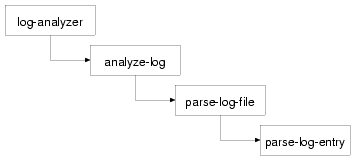
\includegraphics[scale=0.6]{images/restart-call-stack.png}
\end{figure}

Предполагая, что вы всегда хотите пропускать неправильно сформированные записи, вы можете
изменить эту функцию для установки обработчика условия, который вызывает перезапуск
\lstinline{skip-log-entry} для вас. Однако вы не можете использовать \lstinline{HANDLER-CASE} для
установки обработчика условия, потому что тогда стек будет опустошён до функции, где
\lstinline{HANDLER-CASE} появляется. Вместо этого вам надо использовать макрос нижнего уровня
\lstinline{HANDLER-BIND}. Основная форма \lstinline{HANDLER-BIND} следующая:

\begin{myverb}
(handler-bind (binding*) form*)
\end{myverb}

\noindent{}где каждая привязка (binding) представляет собой список из типа условия и
обрабатывающей функции с одним аргументом. После провязок с обработчиками тело
\lstinline{HANDLER-BIND} может содержать произвольное число форм. В~отличие от кода
обработчика в \lstinline{HANDLER-CASE}, код обработчика должен быть функцией и должен
принимать единственный аргумент. Более важным различием между \lstinline{HANDLER-BIND} и
\lstinline{HANDLER-CASE} является то, что функция обработки, привязанная через
\lstinline{HANDLER-BIND}, будет запущена без опустошения стека~-- поток контроля будет всё
ещё в вызове \lstinline{parse-log-entry}, если эта функция вызвана. Вызов
\lstinline{INVOKE-RESTART} найдёт и вызовет последний связанный перезапуск с данным
именем. Таким образом вы можете добавить обработчик к \lstinline{log-analyzer}, который
будет вызывать \lstinline{skip-log-entry} перезапуск, установленный в
\lstinline{parse-log-file}, таким образом\footnote{Компилятор может возмутиться, если
  параметр нигде не используется. Вы можете подавить это предупреждение, добавив
  объявление \lstinline{(declare (ignore c))} как первое выражение в тело
\lstinline{LAMBDA}.}\hspace{\footnotenegspace}:

\begin{myverb}
(defun log-analyzer ()
  (handler-bind ((malformed-log-entry-error
                  #'(lambda (c)
                      (invoke-restart 'skip-log-entry))))
    (dolist (log (find-all-logs))
      (analyze-log log))))
\end{myverb}

В~этом \lstinline{HANDLER-BIND} обработчик является безымянной функцией, которая вызывает
перезапуск \lstinline{skip-log-entry}. Вы также могли бы определить функцию с именем, которая
делала бы то же самое, и связать всё с ней. Фактически это обычная практика, когда
определение перезапуска является определением функции с тем же именем и, получающей
единственный аргумент, условие, которая вызывает одноимённый перезапуск. Такие функции
называются функциями перезапуска. Можно определить функцию перезапуска
\lstinline{skip-log-entry} так:

\begin{myverb}
(defun skip-log-entry (c)
  (invoke-restart 'skip-log-entry))
\end{myverb}

Затем вы могли бы изменить определение \lstinline{log-analyzer} на такое:

\begin{myverb}
(defun log-analyzer ()
  (handler-bind ((malformed-log-entry-error #'skip-log-entry))
    (dolist (log (find-all-logs))
      (analyze-log log))))
\end{myverb}

Как уже было сказано, функция перезапуска \lstinline{skip-log-entry} полагает, что перезапуск
\lstinline{skip-log-entry} уже был установлен. Если \lstinline{malformed-log-entry-error}
просигнализирован кодом, вызванным из \lstinline{log-analyzer} без уже установленного
\lstinline{skip-log-entry}, вызов \lstinline{INVOKE-RESTART} будет сигнализировать
\lstinline{CONTROL-ERROR}, когда не сможет обнаружить перезапуск \lstinline{skip-log-entry}. Если вы
хотите допустить возможность того, чтобы \lstinline{malformed-log-entry-error} могло быть
просигнализировано из кода, в котором перезапуск \lstinline{skip-log-entry} не установлен, то вы
можете изменить функцию \lstinline{skip-log-entry} таким образом:

\begin{myverb}
(defun skip-log-entry (c)
  (let ((restart (find-restart 'skip-log-entry)))
    (when restart (invoke-restart restart))))
\end{myverb}

\lstinline{FIND-RESTART} ищет перезапуск с данным именем и возвращает объект, представ\-ляю\-щий
перезапуск, если перезапуск найден, или \lstinline{NIL}, если нет. Вы можете вызвать перезапуск
путём посылки перезапуск-объекта к \lstinline{INVOKE-RESTART}. Таким образом, когда
\lstinline{skip-log-entry} привязывается внутри \lstinline{HANDLER-BIND}, она будет обрабатывать
условие путём вызова перезапуска \lstinline{skip-log-entry}, если тот доступен, или, в противном
случае, нормально завершится, давая другим обработчикам условия, привязанным выше по
стеку, шанс таки обработать условие.

\section{Предоставление множественных перезапусков}

Так как перезапуски должны быть прямо вызваны, чтобы был какой-то эффект, вы можете
определить несколько перезапусков, предоставляющих различную стратегию исправления. Как я
упоминал ранее, не все приложения для разбора журналов будут обязательно хотеть пропускать
неправильные записи. Некоторые приложения могут захотеть, чтобы \lstinline{parse-log-file}
включала специальный тип объекта для представления неправильной записи в списке
\lstinline{log-entry} объектов; другие приложения могут иметь несколько путей для
восстановления неправильной записи и могут хотеть иметь способ отправки исправленной
записи назад в \lstinline{parse-log-entry}.

Чтобы позволить существовать более сложным протоколам исправления, перезапуски могут
получать произвольные аргументы, которые передаются в вызове \lstinline{INVOKE-RESTART}. Вы
можете предоставить поддержку для обеих стратегий исправления, которые я упомянул, путём
добавления двух перезапусков к \lstinline{parse-log-entry}, каждый из которых получает
единственный аргумент. Первый просто возвращает значение, которое получил, как значение
всего \lstinline{parse-log-entry}, в то время как другой пытается разобрать свой аргумент на
месте оригинальной журнальной записи.

\begin{myverb}
(defun parse-log-entry (text)
  (if (well-formed-log-entry-p text)
    (make-instance 'log-entry ...)
    (restart-case (error 'malformed-log-entry-error :text text)
      (use-value (value) value)
      (reparse-entry (fixed-text) (parse-log-entry fixed-text)))))
\end{myverb}

Имя \lstinline{USE-VALUE} является стандартным именем для такого типа перезапуска. Common Lisp
определяет функцию для \lstinline{USE-VALUE} аналогично \lstinline{skip-log-entry} функции, только
что вами определённой. Таким образом, если вы хотели изменить политику по отношению к
неправильным записям на ту, которая создана экземпляром \lstinline{malformed-log-entry}, вы
могли бы сменить \lstinline{log-analyzer} на такую функцию (предполагая существование
\lstinline{malformed-log-entry} класса с инициирующим аргументом \lstinline{:text}):

\begin{myverb}
(defun log-analyzer ()
  (handler-bind ((malformed-log-entry-error
                  #'(lambda (c)
                      (use-value
                       (make-instance 'malformed-log-entry :text (text c))))))
    (dolist (log (find-all-logs))
      (analyze-log log))))
\end{myverb}

Вы могли бы точно так же поместить эти новые перезапуски в \lstinline{parse-log-file} вмес\-то
\lstinline{parse-log-entry}. Хотя вы, вообще-то, хотите поместить перезапуски в код
по возможности самого нижнего уровня. Не было бы, однако, правильным перемещать перезапуск
\lstinline{skip-log-entry} в \lstinline{parse-log-entry}, так как это может привести к возвращению
иногда \lstinline{'NIL} от \lstinline{parse-log-entry} в качестве результата нормального завершения,
а вы начинали всё с тем, чтобы таких вещей избежать. И это была бы одинаково плохая идея~--
убрать перезапуск \lstinline{skip-log-entry}, исходя из теории, что обработчик условия смог бы
достичь того же эффекта через вызов-перезапуск \lstinline{use-value} с \lstinline{NIL} в качестве
аргумента; это потребовало бы от обработчика условия знания внутренней работы
\lstinline{parse-log-file}. Таким образом, \lstinline{skip-log-entry}~-- правильно абстрагированная
часть API журнального разбора.

\section{Другие применения условий}
\label{ch19:other-appls}

В~то время как условия в основном используются для обработки ошибок, они также могут быть
использованы для других целей~-- вы можете применить условия, обработчики условий и
перезапуски для конструирования различных протоколов между низко- и высокоуровневым
кодом. Ключом для понимания возможностей условий является понимание того, что просто
сигнализация условия не влияет на поток контроля.

Примитивная сигнальная функция \lstinline{SIGNAL} воплощает механизм поиска применимого
обработчика условия и вызывает его обрабатывающую функцию. Причина, почему обработчик
может отказаться обрабатывать условие и нормально завершиться,~-- потому что вызов
функции обработчика,~-- это обычный вызов функции: когда обработчик завершается, контроль
передаётся обратно к \lstinline{SIGNAL}, которая затем ищет другой, ранее привязанный
обработчик, который может обработать условие. Если \lstinline{SIGNAL} исчерпает обработчики
условия до того, как условие будет обработано, она также завершается нормально.

Ранее использованная вами функция \lstinline{ERROR} вызывает \lstinline{SIGNAL}. Если ошибка
обрабатывается обработчиком условия, который передаёт управление через \lstinline{HANDLER-CASE}
или через вызов перезапуска, тогда вызов \lstinline{SIGNAL} никогда не завершится. Но если
\lstinline{SIGNAL} завершается, \lstinline{ERROR} вызывает отладчик путём вызова функции,
сохранённой в \lstinline{*DEBUGGER-HOOK*}. Таким образом, вызов \lstinline{ERROR} никогда не сможет
завершиться нормально; условие должно быть обработано или обработчиком условия, или в
отладчике.

Другая сигнализирующая условие функция \lstinline{WARN} представляет пример протокола ещё
одного типа, построенный на системе условий. Подобно \lstinline{ERROR}, \lstinline{WARN}
вызывает \lstinline{SIGNAL} для сигнализации условия. Но если \lstinline{SIGNAL}
завершается, \lstinline{WARN} не вызывает отладчик~-- она печатает условие в
\lstinline{*ERROR-OUTPUT*} и возвращает \lstinline{NIL}, позволяя своему вызывающему
продолжать работу. \lstinline{WARN} также устанавливает перезапуск
\lstinline{MUFFLE-WARNING}, обёртку вокруг вызова \lstinline{SIGNAL}, которая может быть
использована обработчиком условия, чтобы сделать возврат из \lstinline{WARN} без печатания
чего-либо. Функция \lstinline{MUFFLE-WARNING} перезапуска ищет и вызывает одноимённый
перезапуск, сигнализируя \lstinline{CONTROL-ERROR}, если такого перезапуска нет. Конечно,
условие, сигнализируемое \lstinline{WARN}, также может быть обработано другим путём~--
обработчик условия может <<\textit{поспособствовать}>>, чтобы предупреждение об ошибке
обрабатывалось, как если бы ошибка действительно была.

Например, в приложении для разбора журналов, если журнальная запись немного неправильна, но
всё же поддаётся разбору, вы могли бы указать \lstinline{parse-log-entry} разобрать немного
повреждённую запись, но сигнализировать \lstinline{WARN}, когда она будет делать это. Затем
большее приложение может выбрать либо позволить предупреждению быть напечатанным, либо
скрыть предупреждение, либо рассматривать предупреждение как ошибку, исправляя ситуацию,
как это делалось при \lstinline{malformed-log-entry-error}.

Третья сигнализирующая ошибки функция, \lstinline{CERROR}, представляет ещё один протокол.
Подобно \lstinline{ERROR}, \lstinline{CERROR} сбросит вас в отладчик, если условие, которая она
сигнализирует, не будет обработано. Однако, как и \lstinline{WARN}, она устанавливает перезапуск
перед сигнализацией условия. Перезапуск, \lstinline{CONTINUE}, приведёт к нормальному
завершению \lstinline{CERROR}~-- если перезапуск был вызван обработчиком условия, он вообще
сохранит вас от попадания в отладчик. В~противном случае вы можете использовать
перезапуск, как только окажетесь в отладчике для продолжения вычислений сразу после вызова
\lstinline{CERROR}. Функция \lstinline{CONTINUE} находит и вызывает \lstinline{CONTINUE} перезапуск, если
он доступен, и возвращает \lstinline{NIL} в противном случае.

Вы также можете конструировать ваши собственные протоколы поверх \lstinline{SIGNAL}~-- везде,
где низкоуровневый код нуждается в передаче информации назад по стеку вызовов в
высокоуровневый код, механизм условий является подходящим механизмом для использования. Но
для большинства целей один из стандартных протоколов ошибок или предупреждений должен
подойти.

Вы будете использовать систему условий в будущих практических главах как в виде обычной
обработки ошибок, так и, в \ref{ch:25}-й главе, для помощи в обработке мудрёного особого случая при
разборе ID3-файлов.  К сожалению, это судьба обработки ошибок, всегда идти мелким шрифтом
в программных текстах~-- надлежащая обработка ошибок или отсутствие таковой является
часто наибольшим отличием иллюстративного кода и утяжелённого кода промышленного качества.
Хитрость написания последнего относится больше к принятию особого строгого образа мышления
о программном обеспечении, чем к деталями конструкции языка. Так что если вашей целью
является написание такого типа программ, то вы найдёте систему условий в Common Lisp
отличным инструментом для написания надёжного кода и прекрасно подходящей для стиля
последовательных улучшений (incremental development style).

\textintable{Написание надёжных программ}{Для информации по написанию надёжных программ нет ничего лучше, чем начать с поиска книги
Гленфорда Мейерса <<Надёжность программного обеспечания>> (\textit{Software Reliability},
Glenford J. Meyers, John Wiley \& Sons, 1976).  Написанное Бертрандом Мейером (Bertrand
Meyer) про <<контрактное программирование>> (Design By Contract) также показывает полезный
путь в размышлениях про правильность программ.  Например, смотрите главы~11 и~12 его книги
\textit{Object-Oriented Software Construction} (Prentice Hall, 1997). Запомните, однако,
что Бертранд Мейер является изобретателем Eiffel, статически типизированного
крепостнического и дисциплинарного языка из школы Algol/Ada. Хотя у него есть много умных
мыслей про объектную ориентированность и программную надёжность, всё же существует
довольно большой разрыв между его видением программирования и путём Lisp. Наконец, для
прекрасного обзора большинства проблем, окружающих построение отказоустойчивых систем,
смотрите главу 3 из классической \textit{Transaction Processing: Concepts and Techniques}
(Morgan Kaufmann, 1993) от Джима Грея (Jim Gray) и Андреаса Ройтера (Andreas Reuter).}

В~следующей главе я дам быстрый обзор некоторых из 25 специальных операторов, которых у
вас пока не было шанса использовать, по крайней мере прямо.

%%% Local Variables: 
%%% mode: latex
%%% TeX-master: "pcl-ru"
%%% TeX-open-quote: "<<"
%%% TeX-close-quote: ">>"
%%% End: 


\chapter{Специальные операторы}
\label{ch:20}

\thispagestyle{empty}

Между прочим, наиболее впечатляющим аспектом условной системы, описанной в предыдущей
главе, является то, что если бы она не была частью языка, то она могла бы быть полностью
написана в виде отдельной библиотеки.  Это возможно, поскольку специальные операторы
Common Lisp (когда никто не осуществляет прямого доступа к обработке или выдаче условий)
обеспечивают достаточный уровень доступа к низкоуровневым частям языка, что делает
возможным контроль раскрутки стека (unwinding of the stack).

В~предыдущих главах я обсуждал наиболее часто используемые специальные операторы, но было
бы неправильным ознакомиться только с их частью.  Для этого есть две причины~-- во-первых,
некоторые из редко используемых специальных операторов используются редко просто
потому, что то, что они обрабатывают, обычно не используется в большинстве программ.
Ознакомиться с ними будет полезно хотя бы для того, чтобы вы знали, что они существуют.  А
во-вторых, поскольку 25 специальных операторов (вместе с правилами вычисления вызовов
функций и основными типами данных) составляют основу для остальной части языка, то
знакомство с ними поможет вам понять, как язык устроен.

В~этой главе я буду обсуждать специальные операторы (некоторые вкратце, а некоторые~--
более подробно), так что вы сможете увидеть, как они связаны между собой.  Я буду указывать
на те, которые вы сможете напрямую использовать в вашем коде, на те, которые могут служить
основой для конструкций, которые вы будете использовать все время, а также на те, которые
вы будете редко использовать напрямую, но которые вы сможете использовать в коде,
генерируемом макросами.

\section{Контроль вычисления}

К первой категории специальных операторов относятся три оператора, которые обеспечивают
базовый контроль вычисления выражений. Это \lstinline{QUOTE}, \lstinline{IF} и \lstinline{PROGN}, про
которые я уже рассказывал.  Однако было бы неправильным не отметить то, как каждый из этих
специальных операторов предоставляет контроль за вычислением одной или нескольких форм.
\lstinline{QUOTE} предотвращает вычисление выражения и позволяет вам получить s-выражение в
виде данных. \lstinline{IF} реализует базовый оператор логического выбора, на основе которого
могут быть построены все остальные условные выражения\footnote{Конечно, если бы \lstinline{IF}
  не был специальным оператором, а некоторым другим условным выражением, таким как
  \lstinline{COND}, то вы могли бы реализовать \lstinline{IF} в виде макроса.  На самом деле во
  многих диалектах Lisp, начиная с оригинального Lisp McCarthy, \lstinline{COND} был
  примитивным условным оператором.}\hspace{\footnotenegspace}.  А~\lstinline{PROGN} обеспечивает возможность вычисления
последовательности выражений.

\section{Манипуляции с лексическим окружением}

Наибольший класс специальных операторов составляют операторы, которые манипулируют и
производят доступ к лексическому окружению. \lstinline{LET} и \lstinline{LET*}, которые мы уже
обсуждали, являются примерами специальных операторов, которые манипулируют лексическим
окружением, поскольку они вводят новые лексические связи для переменных.  Любая
конструкция, такая как \lstinline{DO} или \lstinline{DOTIMES}, которая связывает лексические
переменные, будет развёрнута в \lstinline{LET} или \lstinline{LET*}\footnote{Конечно, с технической
  точки зрения эти конструкции также будут развёрнуты в \lstinline{LAMBDA}-выражения,
  поскольку, как я упоминял в главе~\ref{ch:06}, \lstinline{LET} может быть определена (и это
делалось в ранних версиях Lisp) в виде макроса, который развёртывается в запуск анонимной
функции.}\hspace{\footnotenegspace}. Специальный оператор \lstinline{SETQ} является одним из операторов для доступа к
лексическому окружению, поскольку он может быть использован для установки значений
переменных, чьи связи были созданы с помощью \lstinline{LET} и \lstinline{LET*}.

Однако не только переменные могут быть поименованы внутри лексического окружения.  Хотя
большинство функций и определены глобально с использованием \lstinline{DEFUN}, но все равно
возможно создание локальных функций с помощью специальных операторов \lstinline{FLET} и
\lstinline{LABELS}, локальных макросов с помощью \lstinline{MACROLET}, а также специальных видов
макросов (называемых символьными макросами) с помощью \lstinline{SYMBOL-MACROLET}.

Точно так же, как и \lstinline{LET} позволяет вам ввести переменную, чьей областью видимости
будет тело \lstinline{LET}, \lstinline{FLET} и \lstinline{LABELS} позволяют вам определить функцию,
которая будет видна только внутри области видимости \lstinline{FLET} или \lstinline{LABELS}.  Эти
специальные операторы являются очень удобными, если вам нужна локальная функция, которая
является слишком сложной для её определения как \lstinline{LAMBDA}, или если вам нужно вызвать
ее несколько раз.  Оба этих оператора имеют одинаковую форму, которая выглядит так:

\begin{myverb}
(flet (function-definition*)
  body-form*)
\end{myverb}

\noindent{}или так:

\begin{myverb}
(labels (function-definition*)
  body-form*)
\end{myverb}

\noindent{}где каждая из \lstinline{function-definition} имеет следующую форму:

\begin{myverb}
(name (parameter*) form*)
\end{myverb}

Разница между \lstinline{FLET} и \lstinline{LABELS} заключается в том, что имена функций, которые
определены с помощью \lstinline{FLET}, могут использоваться только в теле \lstinline{FLET}, в то
время как имена, определённые с помощью \lstinline{LABELS}, могут использоваться сразу, включая
тела функций, определённых с помощью \lstinline{LABELS}. Таким образом, \lstinline{LABELS} может
определять рекурсивные функции, а \lstinline{FLET}~-- не может.  Может показаться ограничением
то, что \lstinline{FLET} не может быть использован для определения рекурсивных функций, но
Common Lisp предоставляет и \lstinline{FLET}, и \lstinline{LABELS} по той причине, что иногда бывает
полезным иметь возможность написать локальную функцию, которая может вызвать другую функцию
с тем же именем, либо глобальную, либо определённую в охватывающей области видимости.

Внутри тела \lstinline{FLET} или \lstinline{LABELS} вы можете использовать имена определённых
функций, точно так же как и имена любых других функций, включая использование со
спе\-циаль\-ным оператором \lstinline{FUNCTION}.  Поскольку вы можете использовать \lstinline{FUNCTION}
для получения объекта-функции, представляющего функцию, определённую с помощью \lstinline{FLET}
или \lstinline{LABELS}, и поскольку \lstinline{FLET} и \lstinline{LABELS} могут быть в области видимости
других связывающих форм, таких как \lstinline{LET}, то эти функции могут использоваться как
замыкания (closures).

Так как локальные функции могут ссылаться на переменные из охватывающего окружения, то
они могут часто записываться таким образом, чтобы принимать меньше параметров, чем
эквивалентные вспомогательные функции.  Это очень удобно, когда вам необходимо в качестве
параметра-функции передать функцию, которая принимает единственный аргумент. Например, в
следующей функции, которую вы увидите снова в главе~\ref{ch:25}, функция
\lstinline{count-version}, определённая с помощью \lstinline{FLET}, принимает единственный аргумент,
как этого требует функция \lstinline{walk-directory}, но она также может использовать
переменную \lstinline{versions}, заданную охватывающим \lstinline{LET}:

\begin{myverb}
(defun count-versions (dir)
  (let ((versions (mapcar #'(lambda (x) (cons x 0)) '(2 3 4))))
    (flet ((count-version (file)
             (incf (cdr (assoc (major-version (read-id3 file)) versions)))))
      (walk-directory dir #'count-version :test #'mp3-p))
    versions))
\end{myverb}

Эта функция также может быть записана с использованием анонимной функции вместо
использования \lstinline{FLET}, но задание имени делает исходный текст более понятным.

И когда вспомогательная функция должна быть рекурсивной, она не может быть
анонимной\pclfootnote{Сюрпризом может показаться то, что в действительности можно сделать
  анонимную функцию рекурсивной.  Однако вы должны будете использовать достаточно
  эзотеричный механизм, известный как <<Y-комбинатор>>.  Но Y-комбинатор является интересным
  теоретическим результатом, а не средством практического программирования, так что мы
  оставим его за пределами данной книги.}.  Когда вам не нужно определять рекурсивную
вспомогательную функцию как глобальную функцию, то вы можете использовать \lstinline{LABELS}.
Например, следующая функция, \lstinline{collect-leaves}, использует рекурсивную вспомогательную
функцию \lstinline{walk} для прохода по дереву и сбора всех объектов дерева в список, который
затем возвращается \lstinline{collect-leaves} (после его реверсирования):

\begin{myverb}
(defun collect-leaves (tree)
  (let ((leaves ()))
    (labels ((walk (tree)
               (cond
                 ((null tree))
                 ((atom tree) (push tree leaves))
                 (t (walk (car tree))
                    (walk (cdr tree))))))
      (walk tree))
    (nreverse leaves)))
\end{myverb}


Снова отметьте, как внутри функции \lstinline{walk} вы можете ссылаться на переменную
\lstinline{leaves}, объявленную окружающим \lstinline{LET}.

\lstinline{FLET} и \lstinline{LABELS} также являются полезными при раскрытии макросов~-- макрос
может раскрываться в код, который содержит \lstinline{FLET} или \lstinline{LABELS} для создания
функций, которые могут быть использованы внутри тела макроса.  Этот приём может быть
использован либо для введения функций, которые будет вызывать пользователь макроса, либо
для организации кода, генерируемого макросом.  Это может служить примером того, как может
быть определена функция, такая как \lstinline{CALL-NEXT-METHOD}, которая может быть
использована только внутри определения метода.

К той же группе, что \lstinline{FLET} и \lstinline{LABELS}, можно отнести специальный оператор
\lstinline{MACROLET}, который вы можете использовать для определения локальных
макросов. Локальные макросы работают так же, как и глобальные макросы, определённые с
помощью \lstinline{DEFMACRO}, за тем исключением, что они не затрагивают глобального
пространства имён.  Когда вычисляется \lstinline{MACROLET}, то выражения в теле вычисляются с
использованием локального определения макроса, которое, возможно, скрывает глобальное
определение, а также используя локальные определения из окружающих выражений.  Подобно
\lstinline{FLET} и \lstinline{LABELS}, \lstinline{MACROLET} может использоваться напрямую, но оно также
очень удобно для использования кодом, сгенерированным макросом,~-- путём обёртки в
\lstinline{MACROLET} некоторого кода, написанного пользователем, макрос может предоставлять
конструкции, которые могут быть использованы только внутри этого кода, или скрывать
глобально определённый макрос.  Вы увидите примеры использования \lstinline{MACROLET} в
главе~\ref{ch:31}.

В~заключение ещё одним специальным оператором для определения макросов является
\lstinline{SYMBOL-MACROLET}, который определяет специальный вид макросов, называемых
символьными макросами (symbol macro).  Символьные макросы аналогичны обычным, за тем
исключением, что они не могут принимать аргументы и их используют как обычный символ, а
не в листовой записи.  Другими словами, после того как вы определили символьный макрос с
некоторым именем, любое использование этого символа как значения будет раскрыто, и вместо
него будет вычислена соответствующая форма.  Это как раз относится к тому, как макросы,
такие как \lstinline{WITH-SLOTS} и \lstinline{WITH-ACCESSORS}, получают возможность определения
<<переменных>>, которые осуществляют доступ к состоянию определённого объекта.  Например,
следующее выражение \lstinline{WITH-SLOTS}:

\begin{myverb}
(with-slots (x y z) foo (list x y z)))
\end{myverb}

\noindent{}может быть раскрыто в код, который использует \lstinline{SYMBOL-MACROLET}:

\begin{myverb}
(let ((#:g149 foo))
  (symbol-macrolet
      ((x (slot-value #:g149 'x))
       (y (slot-value #:g149 'y))
       (z (slot-value #:g149 'z)))
    (list x y z)))
\end{myverb}

Когда вычисляется выражение \lstinline{(list x y z)}, то символы \lstinline{x},
\lstinline{y} и \lstinline{z} будут раскрыты в соответствующие формы, такие как
\lstinline!(slot-value #:g149 'x)!\footnote{\lstinline{WITH-SLOTS} не обязательно должен
  быть реализован с помощью \lstinline{SYMBOL-MACROLET}~-- в некоторых реализациях,
  \lstinline{WITH-SLOTS} может проходить по коду и раскрывать макрос с \lstinline{x},
  \lstinline{y} и \lstinline{z}, уже заменёнными на соответствующие формы
  \lstinline{SLOT-VALUE}.  Вы можете увидеть, как это делает ваша реализация, с помощью
  следующего выражения:

\begin{myverb}
(macroexpand-1 '(with-slots (x y z) obj (list x y z)))
\end{myverb}

Однако реализации Lisp легче выполнить такую подстановку внутри своего кода, чем кода,
написанного пользователем,~-- чтобы заменить \lstinline{x}, \lstinline{y} и \lstinline{z}
только в случаях, когда они используются как значения, проходчик по коду должен понимать
синтаксис всех специальных операторов и уметь рекурсивно раскрывать все макросы, чтобы
определить, включает ли макрос в раскрытой форме эти символы в позиции значения.
Реализации Lisp имеют соответствующий проходчик по коду, но он относится к той части Lisp,
которая недоступна пользователю языка.}\hspace{\footnotenegspace}.

Символьные макросы наиболее часто используются локально и определяются с помощью
\lstinline{SYMBOL-MACROLET}, но Common Lisp также предоставляет макрос
\lstinline{DEFINE-SYMBOL-MACRO}, который определяет глобальный символьный макрос.  Символьный
макрос, определённый с помощью \lstinline{SYMBOL-MACROLET}, скрывает другие макросы с тем же
именем, определённые с помощью \lstinline{DEFINE-SYMBOL-MACRO} или охватывающих выражений
\lstinline{SYMBOL-MACROLET}.

\section{Локальный поток управления}

Следующие четыре специальных оператора, о которых я буду говорить, также создают и
используют имена в лексическом окружении, но для целей изменения контроля потока, а не для
определения новых функций и макросов. Я упоминал ранее все четыре из этих специальных
операторов, потому что они предоставляют низкоуровневые механизмы, используемые для других
особенностей языка. Вот они: \lstinline{BLOCK}, \lstinline{RETURN-FROM}, \lstinline{TAGBODY} и
\lstinline{GO}. Первые два, \lstinline{BLOCK} и \lstinline{RETURN-FROM}, используются вместе для
написания кода, который совершает выход немедленно из секции кода,~-- я говорил про
\lstinline{RETURN-FROM} в главе~\ref{ch:05}, как о способе немедленного выхода из функции, но
он работает и в более общих случаях, чем тот. Два других \lstinline{TAGBODY} и \lstinline{GO},
предоставляют вполне низкоуровневую \textit{goto} конструкцию, которая составляет основу для всех
высокоуровневых конструкций цикла, которые вы уже видели.

Общий скелет формы \lstinline{BLOCK} таков:

\begin{myverb}
(block name
  form*)
\end{myverb}

\noindent{}\textit{name} является символом и \textit{form*}, это формы языка. Формы выполняются по
порядку, и значение последней формы возвращается как значение всего \lstinline{BLOCK}, если не
использован \lstinline{RETURN-FROM} для возврата из блока ранее. \lstinline{RETURN-FROM} форма, как
вы видели в главе~\ref{ch:05}, состоит из имени блока, из которого выходят, и, по желанию, формы,
которая предоставляет возвращаемое значение.  Когда \lstinline{RETURN-FROM} выполняется, это
является причиной немедленного выхода из упомянутого в нём \lstinline{BLOCK}.  Если
\lstinline{RETURN-FROM} вызван с формой, возвращающей значение, \lstinline{BLOCK} вернёт это
значение; в ином случае \lstinline{BLOCK} вернёт \lstinline{NIL}.

Именем для \lstinline{BLOCK} может быть любой символ, включая \lstinline{NIL}. Многие из стандартных
макросов конструкций контроля, таких как \lstinline{DO}, \lstinline{DOTIMES} и \lstinline{DOLIST},
генерируют код, состоящий из \lstinline{BLOCK}, названного \lstinline{NIL}. Это позволяет вам
использовать макрос \lstinline{RETURN}, который, скорее, является синтаксическим сахаром для
\lstinline!(return-from nil ...)!, чтобы прерывать такие циклы. Так, следующий цикл
напечатает не более десяти случайных чисел, остановившись сразу же, как только достигнет
числа, большего, чем~50:

\begin{myverb}
(dotimes (i 10)
  (let ((answer (random 100)))
    (print answer)
    (if (> answer 50) (return))))
\end{myverb}

Задающие функции макросы, такие как \lstinline{DEFUN}, \lstinline{FLET} и \lstinline{LABELS}, с другой
стороны, оборачивают свои тела в \lstinline{BLOCK} с тем же именем, что и функция. Вот почему
вы можете пользоваться \lstinline{RETURN-FROM} для возврата из функции.

\lstinline{TAGBODY} и \lstinline{GO} имеют такое же отношение друг к другу, как \lstinline{BLOCK} и
\lstinline{RETURN-FROM}: \lstinline{TAGBODY} задаёт контекст, в котором определены имена,
используемые \lstinline{GO}. Скелет \lstinline{TAGBODY} следующий:

\begin{myverb}
(tagbody
  tag-or-compound-form*)
\end{myverb}

\noindent{}где каждая \textit{tag-or-compound-form},~-- это или символ, называемый \textit{тег}, или
непустая списочная форма. Форма выполняется по порядку, и теги игнорируются, кроме случая,
о котором я скоро скажу. После выполнения последней формы в \lstinline{TAGBODY} он
возвращает \lstinline{NIL}. В~любом месте внутри лексической области видимости \lstinline{TAGBODY}
вы можете использовать специальный оператор \lstinline{GO} для немедленного перехода на любой
тег, и выполнение продолжится с формы, следующей за тегом. Например, вы можете написать
простейший бесконечный цикл с \lstinline{TAGBODY} и \lstinline{GO} вроде этого:

\begin{myverb}
(tagbody
 top
   (print 'hello)
   (go top))
\end{myverb}

Заметьте, что в то время как имена тегов должны появляться на верхнем уровне в
\lstinline{TAGBODY}, не заключёнными внутри форм, специальный оператор \lstinline{GO} может
появляться где угодно внутри области видимости \lstinline{TAGBODY}. Это означает, что вы можете
написать цикл, который выполняется случайное число раз, например так:

\begin{myverb}
(tagbody
 top
   (print 'hello)
   (when (plusp (random 10)) (go top)))
\end{myverb}

Ещё более глупый пример \lstinline{TAGBODY}, который показывает вам, что можно иметь множество
тегов в одном \lstinline{TAGBODY}, выглядит так:

\begin{myverb}
(tagbody
 a (print 'a) (if (zerop (random 2)) (go c))
 b (print 'b) (if (zerop (random 2)) (go a))
 c (print 'c) (if (zerop (random 2)) (go b)))
\end{myverb}

Эта форма будет прыгать вокруг случайно печатаемых \textit{a}, \textit{b} и \textit{c} до
тех пор, пока \lstinline{RANDOM} не вернёт~1 и управление, наконец, достигнет конца
\lstinline{TAGBODY}.

\lstinline{TAGBODY} редко используется прямо, так как почти всегда удобнее писать итеративные
конструкции в терминах существующих циклических макросов. Однако он становится удобным для
перевода алгоритмов, написанных на других языках, в Common Lisp либо автоматически, либо
вручную. Примером инструмента автоматического перевода является транслятор
FORTRAN-to-Common Lisp, f2cl, который переводит исходный код на Фортране в исходный код
на Common Lisp, для того чтобы сделать различные библиотеки из Фортрана доступными для
программистов на Common Lisp. Так как многие библиотеки Фортрана были написаны до
революции структурного программирования, они полны операторов \textit{goto}. f2cl
транслятор может просто переводить такие \textit{goto} в \lstinline{GO} внутри соответствующих
\lstinline{TAGBODY}\pclfootnote{Одна версия f2cl доступна как часть
  \href{http://clocc.sourceforge.net/}{Common Lisp Open Code Collection (CLOCC)}. Для
  контраста рассмотрим трюки, к которым авторам f2j, FORTRAN-to-Java транслятора
  пришлось прибегнуть. Хотя Java Virtual Machine (JVM) имеет \textit{goto}-инструкцию, она
  не выражена прямо в Java. Таким образом, чтобы скомпилировать все \textit{goto} из
  Фортрана, они сначала компилируют фортран-код в стандартный java-код с вызовами к 
  классу \textit{dummy} для представления меток и \textit{goto}. Затем они компилируют
  исходник обычным java-компилятором и делают постобработку полученного байт-кода для
  перевода вызовов \textit{dummy} в JVM байт-коды. Умно, но болезненно.}.

Аналогично \lstinline{TAGBODY} и \lstinline{GO} могут быть полезны, когда переводятся алгоритмы,
напи\-сан\-ные или прозой, или диаграммами переходов,~-- например, в классической серии
Дональда Кнута <<Искусство программирования>> он описывает алгоритмы, используя формат
<<рецептов>>: 

\begin{myverb}
step 1, do this; 
step 2, do that; 
step 3, go back to step 2;
\end{myverb}

\noindent{}и так далее. Для примера на странице 142 <<Искусства программирования>>, том~2:
<<Получисленные алгоритмы>>, 3-е изд. (Addison-Wesley, 1998), он описывает алгоритм~S,
который вы увидите в главе~\ref{ch:27}, в такой форме:

\textit{Алгоритм~S} (метод выбора последовательности). Для выбора \textit{n} случайных записей из
множества $N$, где $0 < n <= N$.

\begin{description}
\item[S1. (Инициализировать.)] Установить \lstinline!t <-- 0!, \lstinline!m <-- 0!. (В
  этом алгоритме \lstinline!m! представляет количество записей уже выбранных, а \lstinline!t! общее
  количество записей которые мы просмотрели.);

\item[S2. (Сгенерировать U.)]  Сгенерировать случайное число \lstinline!U!, равномерно
  распределённое между нулём и единицей;

\item[S3. (Проверить.)] Если \lstinline!(N - t)U >= n - m!, то перейти к шагу~\textbf{S5};

\item[S4. (Выбрать.)] Выбрать следующую запись в последовательность и увеличить
\lstinline!m! и \lstinline!t! на~1. Если \lstinline!m < n!, то перейти к шагу~\textbf{S2}; иначе 
последовательность закончена и алгоритм завершается;

\item[S5. (Пропустить.)] Пропустить следующую запись (не включать её в 
последовательность), увеличить \lstinline!t! на~1, и вернуться к шагу~\textbf{S2}.

\end{description}

Это описание может быть легко переведено в  функцию Common Lisp после переименования
нескольких переменных таким образом:

\begin{myverb}
(defun algorithm-s (n max) ; max это N в алгоритме Кнута
  (let (seen               ; t в в алгоритме Кнута
        selected           ; m в алгоритме Кнута
        u                  ; U в алгоритме Кнута
        (records ()))      ; список, где мы сохраняем выбранные записи
    (tagbody
     s1
       (setf seen 0)
       (setf selected 0)
     s2
       (setf u (random 1.0))
     s3
       (when (>= (* (- max seen) u) (- n selected)) (go s5))
     s4
       (push seen records)
       (incf selected)
       (incf seen)
       (if (< selected n)
           (go s2)
           (return-from algorithm-s (nreverse records)))
     s5
       (incf seen)
       (go s2))))
\end{myverb}

Это не самый красивый код, но легко проверить, что это канонический перевод алгоритма
Кнута. Однако этот код, в отличие от прозаического описания у Кнута, может быть запущен и
проверен. Затем вы можете начать рефакторинг, проверяя после каждого изменения, что
функция всё ещё работает\footnote{Так как этот алгоритм зависит от значений, возвращаемых
  \lstinline{RANDOM}, вы, может, захотите проверить его с одним и тем же произвольным
  начальным значением (consistent random seed), которое вы можете получить, привязывая
  \lstinline{*RANDOM-STATE*} к значению (make-random-state nil) для каждого вызова
  \lstinline{algorithm-s}. Например, вы можете сделать проверку для
  \lstinline{algorithm-s} путём выполнения следующего кода:

\begin{myverb}
(let ((*random-state* (make-random-state nil))) (algorithm-s 10 200))
\end{myverb}

Если ваша рефакторизация на каждом шаге была правильна, это выражение должно выдавать один
и тот же список каждый раз.}\hspace{\footnotenegspace}.

Сложив все кусочки, вы, возможно, получите что-то наподобие этого:

\begin{myverb}
(defun algorithm-s (n max)
  (loop for seen from 0
     when (< (* (- max seen) (random 1.0)) n)
     collect seen and do (decf n)
     until (zerop n)))
\end{myverb}

Хотя это может быть не очевидно, что этот код правильно представляет \textit{алгоритм~S},
но если вы пришли к нему посредством серии функций, которые вели себя идентично
оригинальному дословному переводу рецепта Кнута, у вас есть хорошее основание верить, что
он правильный.

\section{Раскрутка стека}

Другим интересным аспектом языка является то, что специальные операторы дают вам контроль
за поведением стека вызовов функций. Например, хотя вы обычно используете
\lstinline{BLOCK} и \lstinline{TAGBODY} для управления потоком выполнения команд внутри
отдельной функции, вы также можете использовать их вместе с замыканиями для выполнения
немедленного нелокального выхода из функции в точку, находящуюся ниже на стеке. Это
происходит потому, что имена \lstinline{BLOCK} и теги \lstinline{TAGBODY} могут быть
окружены любым кодом внутри лексического окружения \lstinline{BLOCK} или
\lstinline{TAGBODY}.  Например, рассмотрим следующую функцию:

\begin{myverb}
(defun foo ()
  (format t "Entering foo~%")
  (block a
    (format t " Entering BLOCK~%")
    (bar #'(lambda () (return-from a)))
    (format t " Leaving BLOCK~%"))
  (format t "Leaving foo~%"))
\end{myverb}

Анонимная функция, переданная \lstinline{bar}б использует \lstinline{RETURN-FROM} для выхода из
\lstinline{BLOCK}. Но это выражение \lstinline{RETURN-FROM} не будет вычислено до тех пор, пока
анонимная функция не будет выполнена с помощью \lstinline{FUNCALL} или \lstinline{APPLY}. Теперь
предположим, что \lstinline{bar} выглядит следующим образом:

\begin{myverb}
(defun bar (fn)
  (format t "  Entering bar~%")
  (baz fn)
  (format t "  Leaving bar~%"))
\end{myverb}

Все равно анонимная функция не будет вызвана. Теперь посмотрим на \lstinline{baz}.

\begin{myverb}
(defun baz (fn)
  (format t "   Entering baz~%")
  (funcall fn)
  (format t "   Leaving baz~%"))
\end{myverb}

И в заключение функция выполняется. Но к чему приведёт вызов \lstinline{RETURN-FROM} из блока,
который находится на несколько уровней выше по стеку? На поверку все работает отлично~--
стек отматывается к той точке, где \lstinline{BLOCK} был создан, и контроль возвращается из
соответствующего выражения \lstinline{BLOCK}. Вызовы \lstinline{FORMAT} в функциях \lstinline{foo},
\lstinline{bar} и \lstinline{baz} демонстрируют это:

\begin{myverb}
CL-USER> (foo)
Entering foo
 Entering BLOCK
  Entering bar
   Entering baz
Leaving foo
NIL
\end{myverb}

Заметьте, что единственным выдаваемым сообщением \lstinline{Leaving . . .} является то, которое
было вставлено после выражения \lstinline{BLOCK} в функции \lstinline{foo}.

Поскольку имена блоков имеют лексическую область видимости, \lstinline{RETURN-FROM} всегда
возвращается из наименьшего охватывающего блока \lstinline{BLOCK} в лексическом окружении, в
котором задана форма \lstinline{RETURN-FROM}, даже если \lstinline{RETURN-FROM} выполняется в
отличающемся динамическом контексте. Например, \lstinline{bar} также может содержать форму
\lstinline{BLOCK} с именем~\lstinline{a}, например вот так:

\begin{myverb}
(defun bar (fn)
  (format t "  Entering bar~%")
  (block a (baz fn))
  (format t "  Leaving bar~%"))
\end{myverb}

Это дополнительное выражение \lstinline{BLOCK} никак не изменит поведение \lstinline{foo}~-- поиск
имён, таких как \lstinline{a}, производится лексически, во время компиляции, а не динамически,
так что дополнительный блок не влияет на работу \lstinline{RETURN-FROM}. И наборот, имя
\lstinline{BLOCK} может быть использовано только тем выражением \lstinline{RETURN-FROM}, которое
задано внутри лексической области видимости выражения \lstinline{BLOCK}; нет никакой
возможности для кода, который определён вне блока, выполнить выход из него, кроме как
выполнение замыкания, которое выполнит \lstinline{RETURN-FROM} из лексического окружения
\lstinline{BLOCK}.

\lstinline{TAGBODY} и \lstinline{GO} работают точно так же, как и \lstinline{BLOCK} и \lstinline{RETURN-FROM}.
Когда вы выполняете замыкание, которое содержит выражение \lstinline{GO}, и \lstinline{GO}
вычисляется, то стек отматывается назад к соответствующей форме \lstinline{TAGBODY} и затем
уже переходит к соответствующему тегу.

Однако имена блоков \lstinline{BLOCK} и теги \lstinline{TAGBODY} достаточно сильно отличаются от
связывания лексических переменных. Как обсуждалось в главе~\ref{ch:06}, лексические
связывания имеют неопределённый экстент (extent), что означает, что связывания не
исчезают даже после того, как связывающая форма будет возвращена. С другой стороны,
выражения \lstinline{BLOCK} и \lstinline{TAGBODY} имеют динамический экстент~-- вы можете выполнить
\lstinline{RETURN-FROM} из \lstinline{BLOCK} или \lstinline{GO} из тега \lstinline{TAGBODY}, только когда
\lstinline{BLOCK} или \lstinline{TAGBODY} находятся на стеке вызова функций. Другими словами,
замыкание, которое захватывает имя блока или тег \lstinline{TAGBODY}, может быть передано вниз
по стеку для последующего выполнения, но оно не может быть возвращено вверх по
стеку. Если вы выполните замыкание, которое будет пытаться выполнить \lstinline{RETURN-FROM} из
\lstinline{BLOCK}, после того как \lstinline{BLOCK} будет завершён, то вы получите
ошибку. Аналогично попытка выполнить \lstinline{GO} для \lstinline{TAGBODY}, которое больше не
существует, также вызовет ошибку\pclfootnote{Это достаточно разумное ограничение~-- не
  совсем понятно, что означает возвращение из формы, которая уже завершилась, если вы,
  конечно, не программист на Scheme. Scheme поддерживает продолжения (continuations)~--
  языковые конструкции, которые позволяют выполнить возврат из одной и той же функции
  более одного раза. Но по разным причинам лишь несколько языков, отличных от Scheme,
  поддерживают этот вид продолжений.}.

Маловероятно, что вам понадобится использовать \lstinline{BLOCK} и \lstinline{TAGBODY} для такого
способа раскрутки стека.  Но вы, скорее всего, будете использовать этот подход как часть
системы условий и рестартов, так что понимание того, как оно работает, поможет вам понять,
что в точности делается при запуске рестарта\footnote{Если вы относитесь к тем людям,
  которые любят знать, как что-то работает, вплоть до мелких деталей, то вы можете
  поразмышлять о том, как вы могли бы реализовать макросы системы условий и рестартов,
  используя \lstinline{BLOCK}, \lstinline{TAGBODY}, замыкания и динамические переменные.}\hspace{\footnotenegspace}.

\lstinline{CATCH} и \lstinline{THROW} являются ещё одной парой специальных операторов, которые
приводят к раскрутке стека.  Вы будете использовать эти операторы ещё реже, чем описанные
выше,~-- они являются наследием ранних версий Lisp, которые не имели в своём составе
систему условий Common Lisp.  Они не должны путаться с конструкциями \lstinline{try/catch} и
\lstinline{try/except} из таких языков, как Java и Python.

\lstinline{CATCH} и \lstinline{THROW} являются динамическими аналогами конструкций \lstinline{BLOCK} и
\lstinline{RETURN-FROM}.  Так что вы используете \lstinline{CATCH} для какого-то кода и затем
используете \lstinline{THROW} для выхода из блока \lstinline{CATCH} с возвратом указанного значения.
Разница заключается в том, что связь между \lstinline{CATCH} и \lstinline{THROW} устанавливается
динамически~-- вместо лексически ограниченного имени метка \lstinline{CATCH} является
объектом, называемым тегом catch, и любое выражение \lstinline{THROW} вычисляется внутри
динамического экстента \lstinline{CATCH}, так что <<выбрасывание>> (throws) этого объекта будет
приводить к раскрутке стека к блоку \lstinline{CATCH} и немедленному возврату.  Так
что вы можете написать новые версии функций \lstinline{foo}, \lstinline{bar} и \lstinline{baz}, используя
\lstinline{CATCH} и \lstinline{THROW} вместо \lstinline{BLOCK} и \lstinline{RETURN-FROM}:

\begin{myverb}
(defparameter *obj* (cons nil nil)) ; некоторый произвольный объект

(defun foo ()
  (format t "Entering foo~%")
  (catch *obj*
    (format t " Entering \lstinline{CATCH}~%")
    (bar)
    (format t " Leaving \lstinline{CATCH}~%"))
  (format t "Leaving foo~%"))

(defun bar ()
  (format t "  Entering bar~%")
  (baz)
  (format t "  Leaving bar~%"))

(defun baz ()
  (format t "   Entering baz~%")
  (throw *obj* nil)
  (format t "   Leaving baz~%"))
\end{myverb}

Заметьте, что нет необходимости передавать замыкание вниз по стеку~-- \lstinline{baz} может
напрямую вызвать \lstinline{THROW}.  Результат будет таким же, как и раньше.

\begin{myverb}
  CL-USER> (foo)
  Entering foo
   Entering \lstinline{CATCH}
    Entering bar
     Entering baz
  Leaving foo
  NIL
\end{myverb}

Однако \lstinline{CATCH} и \lstinline{THROW} слишком динамичные.  И в \lstinline{CATCH}, и в
\lstinline{THROW} форма, предс\-тав\-ляю\-щая тег, вычисляется, что означает, что её значение в
обоих случаях определяется во время выполнения.  Так что если некоторый код в \lstinline{bar}
присвоит новое значение \lstinline{*obj*}, то \lstinline{THROW} в \lstinline{baz} не будет пойман в том
же блоке \lstinline{CATCH}.  Это делает использование \lstinline{CATCH} и \lstinline{THROW} более тяжёлым,
чем \lstinline{BLOCK} и \lstinline{RETURN-FROM}. Единственным преимуществом версии \lstinline{foo},
\lstinline{bar} и \lstinline{baz}, которая использует \lstinline{CATCH} и \lstinline{THROW}, является то, что
нет необходимости передавать замыкание вниз по стеку для возврата из \lstinline{CATCH}~--
любой код, который выполняется внутри динамического экстента \lstinline{CATCH}, может заставить
вернуться к нему путём <<бросания>>  нужного объекта.

В~старых диалектах Lisp, в которых не было ничего подобного системе условий Common Lisp,
\lstinline{CATCH} и \lstinline{THROW} использовались для обработки ошибок.  Однако, для того чтобы
сделать её сопровождаемой, теги catch обычно были закавыченными символами, так что вы могли
понять, глядя на \lstinline{CATCH} и \lstinline{THROW}, где они будут перехвачены во время
выполнения. В~Common Lisp вы будете редко иметь нужду в использовании \lstinline{CATCH} и
\lstinline{THROW}, поскольку система условий намного более гибкая.

Последним специальным оператором, относящимся к управлению стеком вызовов, является
\lstinline{UNWIND-PROTECT}, который я вскользь упоминал раньше. \lstinline{UNWIND-PROTECT} позволяет
вам контролировать, что происходит при раскрутке стека, и быть уверенным в том, что
определённый код всегда выполняется, независимо от того, как поток выполнения покидает
область видимости \lstinline{UNWIND-PROTECT}~-- обычным способом, путём запуска рестарта или
любым другим способом, описанным в этом разделе\footnote{\lstinline{UNWIND-PROTECT} является
  эквивалентом конструкции \lstinline{try/finally} в Java и Python.}\hspace{\footnotenegspace}.  Базовая форма
\lstinline{UNWIND-PROTECT} выглядит примерно так:

\begin{myverb}
(unwind-protect protected-form
  cleanup-form*)
\end{myverb}

Сначала вычисляется одиночное выражение \lstinline{protected-form}, и затем, вне зависимости от
способа его завершения, будут вычислены выражения, заданные \lstinline{cleanup-forms}.  Если
\lstinline{protected-form} завершается нормальным образом, то его результат будет возвращён,
\lstinline{UNWIND-PROTECT} после вычисления возвратит \lstinline{cleanup-forms}. Выражения
\lstinline{cleanup-forms} вычисляются в том же самом динамическом окружении, что и
\lstinline{UNWIND-PROTECT}, так что все динамические переменные, связи, перезапуски и
обработчики условий будут доступны коду \lstinline{cleanup-forms}, так как они были видны
перед выполнением \lstinline{UNWIND-PROTECT}.

Вы редко будете использовать \lstinline{UNWIND-PROTECT} напрямую.  Наиболее часто вы его
будете использовать как основу для макросов в стиле \lstinline{WITH-}, таких как
\lstinline{WITH-OPEN-FILE}, который вычисляет произвольное количество выражений в контексте,
где они имеют доступ к некоторому ресурсу, который должен быть освобождён после того, как
все выполнено, вне зависимости от того, как выражения были завершены~-- нормальным
образом, через рестарт или любой другой нелокальный выход.  Например, если вы пишете
библиотеку для работы с базами данных, которая определяет функции \lstinline{open-connection} и
\lstinline{close-connection}, то вы можете написать вот такой макрос\footnote{На самом
  деле CLSQL, интерфейс к множеству баз данных, работающий на многих реализациях Lisp,
  предоставляет макрос с аналогичной функциональностью, имеющий имя \lstinline{with-database}.
  Домашняя страница CLSQL находится по адресу \url{http://clsql.b9.com}.}\hspace{\footnotenegspace}:

\begin{myverb}
(defmacro with-database-connection ((var &rest open-args) &body body)
  `(let ((,var (open-connection ,@open-args)))
    (unwind-protect (progn ,@body)
      (close-connection ,var))))
\end{myverb}

\noindent{}что позволяет вам писать в следующем стиле:

\begin{myverb}
(with-database-connection (conn :host "foo" :user "scott" :password "tiger")
  (do-stuff conn)
  (do-more-stuff conn))
\end{myverb}

\noindent{}и не беспокоиться о закрытии соединения к базе данных, поскольку \lstinline{UNWIND-PROTECT}
позаботится о его закрытии вне зависимости от того, что случится в теле формы
\lstinline{with-database-connection}.

\section{Множественные значения}

Еще одним свойством Common Lisp, которое я упоминал вскользь в главе~\ref{ch:11}, когда
обсуждал \lstinline{GETHASH}, является возможность возвращения множества значений из одного
выражения. Сейчас мы обсудим эту функциональность более подробно. Правда, не совсем
правильно обсуждать эту функциональность в главе про специальные операторы, поскольку данный
функционал не реализуется отдельными операторами, а глубоко интегрирован в
язык. Операторами, которые вы наиболее часто будете использовать с множественными
значениями, являются макросы и функции, а не специальные операторы.  Но базовая
возможность получения множественных значений обеспечивается специальным оператором
\lstinline{MULTIPLE-VALUE-CALL}, на основе которого построен более часто используемый макрос
\lstinline{MULTIPLE-VALUE-BIND}.

Ключом к понимаю множественных значений является тот факт, что возврат множества значений
совершенно отличается от возврата списка: если форма возвращает множество значений, то
до тех пор, пока вы не сделаете что-то специальное для их получения, все значения, кроме
первого (основного), будут игнорироваться.  Для того чтобы увидеть это отличие, рассмотрим
функцию \lstinline{GETHASH}, которая возвращает два значения: найденное значение и логическое
значение, которое равно \lstinline{NIL}, если значение не было найдено.  Если бы эти значения
возвращались в виде списка, то при каждом вызове \lstinline{GETHASH} вам требовалось бы
выделять найденное значение из списка, вне зависимости от того, нужно вам второе
возвращаемое значение или нет.  Предположим, что у вас есть хэш-таблица \lstinline{*h*},
которая содержит числа.  Если бы \lstinline{GETHASH} возвращал список, то вы бы не могли
написать что-то подобное:

\begin{myverb}
(+ (gethash 'a *h*) (gethash 'b *h*))
\end{myverb}

\noindent{}поскольку \lstinline{+} ожидает, что его аргументами будут числа, а не
списки. Но так как механизм работы с множественными значениями просто игнорирует
дополнительные возвращаемые значения, которые вам не нужны, то этот код будет работать
нормально.

Имеются два аспекта использования множественных значений~-- возврат мно\-жес\-твен\-ных
значений и получение неосновных значений, возвращаемых формами, которые возвращают
множественные значения.  Начальной точкой для возврата мно\-жес\-твен\-ных значений являются
функции \lstinline{VALUES} и \lstinline{VALUES-LIST}.  Это обычные функции, а не специальные
операторы, поскольку их параметры передаются как обычно.  \lstinline{VALUES} принимает переменное
число аргументов и возвращает их как множественные значения; \lstinline{VALUES-LIST} принимает
единственный аргумент~-- список значений,~-- и возвращает все его содержимое в виде
множественных значений.  Иначе говоря:

\begin{myverb}
  (values-list x) === (apply #'values x)
\end{myverb}

Механизм возврата множественных значений зависит от конкретной реализации, так же как и
механизм передачи аргументов функциям.  Почти все языковые конструкции, возвращающие
значения своих подвыражений, будут <<передавать>> множественные значения, возвращаемые
подвыражениями.  Так что функция, которая возвращает результат вызова \lstinline{VALUES} или
\lstinline{VALUES-LIST}, сама будет возвращать множественные значения, и то же самое будет
делать и функция, вызвавшая эту функцию, и т.~д.\footnote{Небольшой набор макросов не
  передаёт дополнительные возвращаемые значения тех выражений, которые они вычисляют.  В
  частности, макрос \lstinline{PROG1}, который вычисляет некоторое количество выражений,
  подобно \lstinline{PROGN}, но возвращает значение первого выражения, возвращает только
  основное значение.  Аналогичным образом \lstinline{PROG2}, который возвращает значение
  второго выражения, также возвращает лишь основное значение.  Специальный оператор
  \lstinline{MULTIPLE-VALUE-PROG1} является вариантом \lstinline{PROG1}, который возвращает все
  значения первого выражения.  Это небольшой недостаток, что \lstinline{PROG1} не ведёт себя
  так же, как \lstinline{MULTIPLE-VALUE-PROG1}, но ни один из них не используется достаточно
  часто, чтобы это было неудобным.  Макросы \lstinline{OR} и \lstinline{COND} также не всегда
  прозрачны для множественных значений, возвращая только основное значение определённого
  выражения.}\hspace{\footnotenegspace}.

Но когда выражение вычисляется в позиции значения, то используется только основное
значение~-- вот почему предыдущий пример с добавлением работает, как ожидается. Специальный
оператор \lstinline{MULTIPLE-VALUE-CALL} предоставляет механизм, который позволяет вам работать
с множественными значениями, возвращаемыми выражениями. \lstinline{MULTIPLE-VALUE-CALL}
аналогичен \lstinline{FUNCALL}, за тем исключением, что \lstinline{FUNCALL} является обычной
функцией и, как следствие, использует только основное значение из переданных аргументов,
в то время как \lstinline{MULTIPLE-VALUE-CALL} передаёт функции, указанной в качестве первого
аргумента, все значения, возвращённые остальными выражениями, указанными в качестве
аргументов.

\begin{myverb}
(funcall #'+ (values 1 2) (values 3 4))             ==> 4
(multiple-value-call #'+ (values 1 2) (values 3 4)) ==> 10
\end{myverb}

Но, скорее всего, вы достаточно редко будете просто передавать все значения, возвращённые
одной функцией, в другую функцию.  Скорее всего, вы захотите сохранить множественные
значения в отдельные переменные и затем что-то сделать с ними.  Макрос
\lstinline{MULTIPLE-VALUE-BIND}, с которым вы встречались в главе~\ref{ch:11}, является
наиболее часто используемым оператором для работы с множественными значениями.  В~общем
виде он выглядит вот так:

\begin{myverb}
(multiple-value-bind (variable*) values-form
  body-form*)
\end{myverb}

Выражение \lstinline{values-form} вычисляется, и множественные значения, которые возвращаются
им, присваиваются указанным переменным.  Затем вычисляются выражения \lstinline{body-forms}
при использовании указанных переменных.  Так что:

\begin{myverb}
(multiple-value-bind (x y) (values 1 2)
  (+ x y)) ==> 3
\end{myverb}

Другой макрос~-- \lstinline{MULTIPLE-VALUE-LIST}, ещё более простой~-- он принимает одно
выражение, вычисляет его и собирает полученные множественные значения в список.  Другими
словами, этот макрос выполняет действия, обратные действию\lstinline{VALUES-LIST}.

\begin{myverb}
CL-USER> (multiple-value-list (values 1 2))
(1 2)
CL-USER> (values-list (multiple-value-list (values 1 2)))
1
2
\end{myverb}

Однако если вы обнаружите, что часто используете \lstinline{MULTIPLE-VALUE-LIST}, то это может
быть сигналом того, что некоторая функция должна возвращать список, а не мно\-жес\-твенные
значения.

И в заключение если вы хотите присвоить множественные значения, возвращённые формой,
существующим переменным, то вы можете использовать функцию \lstinline{VALUES} для выполнения
\lstinline{SETF}.  Например:

\begin{myverb}
CL-USER> (defparameter *x* nil)
*X*
CL-USER> (defparameter *y* nil)
*Y*
CL-USER> (setf (values *x* *y*) (floor (/ 57 34)))
1
23/34
CL-USER> *x*
1
CL-USER> *y*
23/34
\end{myverb}

\section{EVAL-WHEN}

Еще одним специальным оператором, принципы работы которого вам нужно понимать, для того
чтобы писать некоторые виды макросов, является \lstinline{EVAL-WHEN}.  По некоторым
причинам книги о Lisp часто считают \lstinline{EVAL-WHEN} орудием только для экспертов.
Но единственным требованием для понимания \lstinline{EVAL-WHEN} является понимание того,
как взаимодействуют две функции~-- \lstinline{LOAD} и \lstinline{COMPILE-FILE}.  И
понимание принципов работы \lstinline{EVAL-WHEN} будет важным для вас, когда вы начнёте
писать сложные макросы, такие как те, которые мы будем писать в главах~\ref{ch:24}
и~\ref{ch:31}.

В~предыдущих главах я немного касался вопросов совместной работы \lstinline{LOAD} и
\lstinline{COMPILE-FILE}, но стоит рассмотреть этот вопрос снова.  Задачей \lstinline{LOAD} являются
загрузка файла и вычисление всех выражений верхнего уровня, содержащихся в нем.  Задачей
\lstinline{COMPILE-FILE} является компиляция исходного текста в файл FASL, который может быть
затем загружен с помощью \lstinline{LOAD}, так что \lstinline{(load "foo.lisp")} и 
\lstinline{(load "foo.fasl")} являются практически эквивалентными.

Поскольку \lstinline{LOAD} вычисляет каждое выражение до чтения следующего, побочный эффект
вычисления выражений, находящихся ближе к началу файла, может воздействовать на то, как
будут читаться и вычисляться формы, находящиеся дальше в файле.  Например, вычисление
выражения \lstinline{IN-PACKAGE} изменяет значение переменной \lstinline{*PACKAGE*}, что затронет
процедуру чтения всех остальных выражений\footnote{Причиной того, что загрузка файла с
  выражением \lstinline{IN-PACKAGE} в нем не имеет никакого влияния на значение
  \lstinline{*PACKAGE*} после возврата из \lstinline{LOAD}, является то, что \lstinline{LOAD} связывает
  \lstinline{*PACKAGE*} со своим текущим значением до того, как сделать что-то иное.  Говоря
  другими словами, что-то подобное следующему выражению \lstinline{LET} окружает остальной код
  в реализации \lstinline{LOAD}:

\begin{myverb}
(let ((*package* *package*)) ...)
\end{myverb}

Любые изменения \lstinline{*PACKAGE*} будут применяться к новой привязке, а старая привязка
будет восстановлена при выходе из \lstinline{LOAD}.  Аналогичным образом эта функция связывает
переменную \lstinline{*READTABLE*}, которую мы ещё не обсуждали.}\hspace{\footnotenegspace}.  Аналогичным образом
выражение \lstinline{DEFMACRO}, находящееся раньше в файле, может определить макрос, который
будет использоваться кодом, находящимся далее в файле\footnote{В~некоторых реализациях вы
  можете избежать вычисления \lstinline{DEFUN}, которые используют
  неопределённые макросы в теле функции, поскольку макросы определяются до того, как
  функция будет вызвана.  Но это будет работать только в тех случаях, когда вы загружаете
  определения с помощью \lstinline{LOAD} из файла с исходным кодом, но не компилируете с
  помощью \lstinline{COMPILE-FILE}, так что, в общем, определения макросов должны быть вычислены
  до того, как они будут использованы.}\hspace{\footnotenegspace}.

С другой стороны, \lstinline{COMPILE-FILE} обычно не вычисляет выражения в процессе компиляции;
это происходит в момент загрузки файла FASL. Однако \lstinline{COMPILE-FILE} должен вычислять
некоторые выражения, такие как \lstinline{IN-PACKAGE} и \lstinline{DEFMACRO}, чтобы поведение
\lstinline{(load "foo.lisp")} и \lstinline{(load "foo.fasl")} было консистентным.

Так как же работают макросы, такие как \lstinline{IN-PACKAGE} и \lstinline{DEFMACRO}, в тех случаях,
ког\-да они обрабатываются \lstinline{COMPILE-FILE}?  В~некоторых версиях Lisp, существовавших до
разработки Common Lisp, компилятор файлов просто знал, что он должен вычислять некоторые
макросы в добавление к их компиляции.  Common Lisp избегает необходимости таких хаков
путём введения специального оператора \lstinline{EVAL-WHEN}, взятого из Maclisp.  Этот оператор,
как и предполагает его имя, позволяет контролировать то, когда определённые части кода
должны вычисляться. В~общем виде выражение \lstinline{EVAL-WHEN} выглядит вот так:

\begin{myverb}
(eval-when (situation*)
  body-form*)
\end{myverb}

Есть три возможных условия~-- \lstinline{:compile-toplevel}, \lstinline{:load-toplevel}
и \lstinline{:execute}, и то, которое вы укажете, будет определять то, когда будут вычислены
выражения, указанные \lstinline{body-forms}.  \lstinline{EVAL-WHEN} с несколькими условиями
аналогичен записи нескольких выражений \lstinline{EVAL-WHEN} с разными условиями, но с
одинаковыми выражениями.  Для объяснения того, что означают эти условия, нам необходимо
объяснить, что делает \lstinline{COMPILE-FILE} (который также называют компилятором файлов) в
процессе компиляции файла.

Для того чтобы объяснить, как \lstinline{COMPILE-FILE} компилирует выражения
\lstinline{EVAL-WHEN}, я должен описать отличия между компиляцией выражений верхнего
уровня (top-level form) и компиляцией остальных выражений.  Выражения верхнего уровня,
грубо говоря~-- это те, которые будут скомпилированы в исполняемый код, который будет
выполнен при загрузке файла FASL.  Так что все выражения, которые находятся на верхнем
уровне файла с исходным текстом, будут скомпилированы как выражения верхнего
уровня. Аналогичным образом все выражения, указанные в выражении \lstinline{PROGN}
верхнего уровня, будут также скомпилированы как выражения верхнего уровня
(\lstinline{PROGN} сам ничего не делает~-- он лишь группирует вместе указанные выражения),
и они будут выполнены при загрузке FASL\footnote{В~противоположность этому выражения,
  указанные в \lstinline{LET} верхнего уровня, не будут скомпилированы как выражения
  верхнего уровня, потому что они не будут выполняться при загрузке FASL.  Они будут
  выполнены в контексте привязок, созданных \lstinline{LET}. Теоретически \lstinline{LET},
  не связывающий никаких переменных, может рассматриваться как \lstinline{PROGN}, но это не
  так~-- выражения, указанные в \lstinline{LET}, никогда не будут считаться выражениями
  верхнего уровня.}\hspace{\footnotenegspace}.  Аналогичным образом выражения, указанные в \lstinline{MACROLET} или
\lstinline{SYMBOL-MACROLET}, будут скомпилированы как выражения верхнего уровня, поскольку
после того, как компилятор раскроет локальные и символьные макросы, в скомпилированном
коде не останется никаких упоминаний \lstinline{MACROLET} или \lstinline{SYMBOL-MACROLET}.
И в заключение раскрытие макроса верхнего уровня будет скомпилировано как выражение
верхнего уровня.

Таким образом, \lstinline{DEFUN}, указанный на верхнем уровне исходного текста, является
выражением верхнего уровня~-- код, который определяет функцию и связывает её с именем,
будет выполнен при загрузке FASL, но выражения внутри тела функции, которые не будут
выполнены до тех пор, пока функция не будет вызвана, не являются вы\-ра\-же\-ния\-ми верхнего
уровня.  Большинство выражений компилируется одинаково вне зависимости от того, на верхнем
они уровне или нет, но семантика выражения \lstinline{EVAL-WHEN} зависит от того, будет ли
оно скомпилировано как выражение верхнего уровня, выражение неверхнего уровня или просто
вычислено, и все это в комбинации с условиями, указанными в выражении.

Условия \lstinline{:compile-toplevel} и \lstinline{:load-toplevel} контролируют поведение
\lstinline{EVAL-WHEN}, которое компилируется как выражение верхнего уровня.  Когда присутствует
условие \lstinline{:compile-toplevel}, то компилятор файла вычислит заданные выражения во время
компиляции.  Когда указано условие \lstinline{:load-toplevel}, то он будет компилировать
выражения как выражения верхнего уровня.  Если ни одно из этих условий не указано в
выражении \lstinline{EVAL-WHEN} верхнего уровня, то компилятор просто игнорирует его.

Когда \lstinline{EVAL-WHEN} компилируется как выражение не верхнего уровня, то он либо
компилируется как \lstinline{PROGN}, в том случае если указано условие
\lstinline{:execute}, либо просто игнорируется.  Аналогичным образом вычисляемое
выражение \lstinline{EVAL-WHEN} (что включает в себя выражения \lstinline{EVAL-WHEN}
верхнего уровня в исходном тексте, обрабатываемом \lstinline{LOAD}, и
\lstinline{EVAL-WHEN}, вычисляемый во время компиляции, когда он является подвыражением
другого \lstinline{EVAL-WHEN} с условием \lstinline{:compile-toplevel}) также
рассматривается как \lstinline{PROGN}, если указано условие \lstinline{:execute}, и
игнорируется в противном случае.

Таким образом, макрос, такой как \lstinline{IN-PACKAGE}, может производить необходимые действия
и во время компиляции, и при загрузке из исходного кода путём раскрытия в выражения
\lstinline{EVAL-WHEN}, выглядящие примерно так:

\begin{myverb}
(eval-when (:compile-toplevel :load-toplevel :execute)
  (setf *package* (find-package "PACKAGE-NAME")))
\end{myverb}

Значение \lstinline{*PACKAGE*} будет выставлено во время компиляции из-за условия
\lstinline{:compile-toplevel}, во время загрузки FASL из-за условия \lstinline{:load-toplevel} и во
время загрузки исходного кода из-за условия \lstinline{:execute}.

Существуют два широко распространённых способа использования \lstinline{EVAL-WHEN}. Первый~--
если вы хотите написать макрос, которому необходимо сохранить некоторую информацию во
время компиляции и которая будет использоваться при генерации раскрытий других
макровыражений в том же файле.  Это обычно нужно для определяющих (definitional)
макросов, когда определение, расположенное в начале файла, могут влиять на код,
генерируемый для определения, расположенного далее в том же файле.  Вы будете писать такие
макросы в главе~\ref{ch:24}.

Вам также может понадобиться использовать \lstinline{EVAL-WHEN}, если вы захотите поместить
определение макроса и вспомогательной функции, которая используется в этом макросе, в том
же файле с исходным текстом, что и код, использующий данный макрос. \lstinline{DEFMACRO} уже
использует \lstinline{EVAL-WHEN} в своём раскрытии, так что определение макроса становится
доступным для использования сразу.  Но обычно \lstinline{DEFUN} не делает определение функции
доступным во время компиляции, а если вы используете макрос в том же файле, где он
определён, то вам необходимо, чтобы были определены и все функции, используемые в
макросе. Если вы обернёте все определения вспомогательных функций в выражение
\lstinline{EVAL-WHEN} с условием \lstinline{:compile-toplevel}, то определения будут доступны при
раскрытии макросов. Вы, наверное, захотите включить также условия \lstinline{:load-toplevel} и
\lstinline{:execute}, поскольку макросы будут требовать наличия определения функций после того,
как файл скомпилирован и загружен, или если вы загружаете файл с исходным текстом вместо
компиляции.

\section{Другие специальные операторы}

Все оставшиеся четыре специальных оператора~-- \lstinline{LOCALLY}, \lstinline{THE},
\lstinline{LOAD-TIME-VALUE} и \lstinline{PROGV},~-- позволяют получить доступ к некоторым
частям нижележащего языка, к которым доступ не может быть осуществлён другими способами.
\lstinline{LOCALLY} и \lstinline{THE} являются частями системы объявлений Common Lisp,
которая используется для <<связывания>> некоторых вещей с компилятором, что не изменит
работу вашего кода, но позволит генерировать лучший код~-- более быстрый, более понятные
сообщения об ошибках и т.~п\footnote{Одним из объявлений, которая имеет влияние на
  семантику программы, является объявление \lstinline{SPECIAL}, упомянутое в
  главе~\ref{ch:06}.}\hspace{\footnotenegspace}. Мы коротко обсудим объявления в
главе~\ref{ch:32}.

Еще два оператора~-- \lstinline{LOAD-TIME-VALUE} и \lstinline{PROGV},~-- используются редко, и
объяснение того, почему это происходит, займёт больше времени, чем объяснение того, что
они делают. Я расскажу вам то, что они делают, так что просто вы будете иметь эту
информацию. Когда-нибудь вы встретите один из них, и тогда вы будете готовы к пониманию их
работы.

\lstinline{LOAD-TIME-VALUE} используется (как видно из его имени) для создания значения во
время загрузки.  Когда компилятор обрабатывает код, который содержит выражение
\lstinline{LOAD-TIME-VALUE}, он генерирует код, который выполнит подвыражения лишь один раз, во
время загрузки FASL, и код, содержащий выражение \lstinline{LOAD-TIME-VALUE}, будет ссылаться на
вычисленное значение.  Другими словами, вместо того чтобы писать что-то подобное:

\begin{myverb}
(defvar *loaded-at* (get-universal-time))

(defun when-loaded () *loaded-at*)
\end{myverb}

\noindent{}вы можете просто написать вот так:

\begin{myverb}
(defun when-loaded () (load-time-value (get-universal-time)))
\end{myverb}

В~коде, не обрабатываемом \lstinline{COMPILE-FILE}, выражение \lstinline{LOAD-TIME-VALUE}
вычисляется однажды, во время компиляции, что может происходить, когда вы явно компилируете
функцию с помощью \lstinline{COMPILE}, или даже раньше, из-за неявной компиляции кода во время
его вычисления.  В~некомпилируемом коде \lstinline{LOAD-TIME-VALUE} вычисляет свои
подвыражения при каждом вычислении.

И в заключение \lstinline{PROGV} создаёт новые динамические привязки для переменных, чьи имена
определяются во время выполнения.  Это в основном полезно при реализации встраиваемых
интерпретаторов для языков с динамической областью видимости переменных.  Базовая
структура этого выражения выглядит вот так:

\begin{myverb}
(progv symbols-list values-list
  body-form*)
\end{myverb}

\noindent{}где \lstinline{symbols-list} является выражением, которое вычисляется в список символов, а
\lstinline{values-list}~-- выражение, которое вычисляется в список значений.  Каждый символ
динамически связывается с соответствующим значением, и затем вычисляются выражения,
указанные в \lstinline{body-forms}.  Разница между \lstinline{PROGV} и \lstinline{LET} заключается в том,
что \lstinline{symbols-list} вычисляется во время выполнения и имена связываемых переменных
вычисляются динамически.  Как я уже сказал, этот оператор не понадобится вам очень часто.

И это вся информация о специальных операторах.  В~следующей главе я вернусь к
практическим темам и покажу вам, как использовать пакетную систему Common Lisp для
получения контроля за пространствами имён, так что вы можете писать библиотеки и
приложения, которые смогут сосуществовать без разрушения друг друга.

%%% Local Variables: 
%%% mode: latex
%%% TeX-master: "pcl-ru"
%%% TeX-open-quote: "<<"
%%% TeX-close-quote: ">>"
%%% End: 


\chapter{Программирование по-взрослому: Пакеты и Символы}
\label{ch:21}

В 4-й главе я рассказывал, как считыватель Lisp переводит текстовые имена в объекты,
которые затем передаются вычислителю в виде так называемых \textit{символов}.
Оказывается, что иметь встроенный тип данных, специально для представления имён, очень
удобно для многих видов программирования.\footnote{Способ программирования, основывающийся
  на типе данных \textit{символ}, называется, вполне подходяще, \textit{символьной}
  обработкой. Обычно он противопоставляется \textit{численному} программированию.  Пример
  программы, с которой должны быть хорошо знакомы все программисты и которая занимается
  почти исключительно символьными преобразованиями - компилятор. Он принимает текст
  программы, как набор символов и преобразует его в новую форму.} Это, однако, не тема
данной главы. В этой главе я расскажу об одном из наиболее явных и практических аспектов
работы с именами: как избегать конфликта между независимо разрабатываемыми кусками кода.

Предположим, для примера, что вы пишете программу и решаете использовать чью-то
библиотеку.  Вы не хотите знать имена всех функций, переменных, классов или макросов
внутри этой библиотеки, чтобы избежать путаницы между её именами и именами, которые вы
используете в своей программе. Вы бы хотели, чтобы большинство имён в библиотеке и имён в
вашей программе рассматривались отдельно, даже если они окажутся одинаковыми в написании.
В то же самое время, вы хотите, чтобы некоторые имена, определённые в библиотеке, были
легко доступны -- те имена, что составляют её публичный API, который вы как раз хотите
использовать.

В Common Lisp эта проблема пространства имён сводится просто к вопросу контроля за тем,
как считыватель переводит текстовые имена в символы: если вы хотите чтобы два появления
одного и того же имени рассматривались интерпретатором одинаково, вы должны убедиться, что
считыватель использует один и тот же символ для представления каждого из них. И наоборот,
если нужно, чтобы два имени рассматривались как разные, даже если они совпадают
побуквенно, вам надо, чтобы считыватель создал разные символы для представления этих имён.

\section{Как считыватель использует пакеты}

В главе~\ref{ch:04} я коротко рассказал, как считыватель в LISP переводит имена в символы,
но я пропустил множество деталей -- теперь настало время поближе взглянуть на то, что же
происходит на самом деле.

Начну с описания синтаксиса имён, понимаемых считывателем, и того, как он соотносится с
пакетами.  На данный момент можете представить себе пакеты, как таблицы, которые
отображают строки в символы. Как вы увидите в дальнейшем, в действительности это
отображение можно регулировать более тонко, чем в простой таблице соответствий, но не теми
способами, которые использует считыватель. Каждый пакет также имеет имя, которое может
быть использовано для поиска пакета через функцию \code{FIND-PACKAGE}.

Две ключевые функции, которые считыватель использует для доступа к отображению
имя-в-символ в пакете, это \code{FIND-SYMBOL} и \code{INTERN}. Обе они получают строку и,
необязательно, пакет.  Если пакет не указывается, на его место подставляется значение
глобальной переменной \code{*PACKAGE*}, называемой также \textit{текущим пакетом}.

\code{FIND-SYMBOL} ищет в пакете символ с именем, совпадающим со строкой, и возвращает его
или \code{NIL}, если символ не найден. \code{INTERN} также возвратит существующий символ,
но если его нет, создаст новый, назначит строку его именем и поместит в пакет.

Большинство имён используемых вами -- неспециализированные имена, не содержащие
двоеточий. Когда считыватель читает такое имя, он переводит его в символ путём изменения
всех не экранированных букв в верхний регистр и передавая полученную строку \code{INTERN}.
Таким образом каждый раз, когда считыватель читает то же имя в том же пакете, он получает
тот же объект-символ. Это важно, так как интерпретатор использует объектное совпадение
символов, чтобы определить к какой функции, переменной или другому программному элементу
данный символ относится. То есть причина, по которой выражение вида \code{(hello-world)}
преобразуется в вызов определённой hello-world фукции, это возврат считывателем одного и
того же символа, и когда он читает вызов функции, и когда он он читал форму \code{DEFUN},
которая эту функцию определяла.  Имя, содержащее двоеточие или двойное двоеточие, является
пакетно-специализированным именем. Когда считыватель читает пакетно-специализированное
имя, он разбивает его в месте двоеточия(й) и берёт первую часть, как имя пакета, а вторую
как имя символа.  Затем считыватель просматривает соответствующий пакет и использует его
для перевода имени в символ-объект.

Имена, содержащие только одинарное двоеточие, относятся к внешним символам, тем, которые
пакет экспортирует для общего пользования. Если названный пакет не содержит символа с
данным именем, или содержит, но он не экспортирован, считыватель сигнализирует об
ошибке. Имена с двойным двоеточием могут обозначать любой символ в названном пакете, хотя
это обычно плохой тон -- множество экспортированных символов определяют публичный
интерфейс пакета и, если вы не уважаете решение автора пакета о том, какие имена делать
внешними, а какие внутренними, вы напрашиваетесь на неприятности в дальнейшем. С другой
стороны, иногда авторы пакетов забывают экспортировать символы, явно предназначенные для
внешнего пользователя. В таком случае имена с двойным двоеточием позволят вам работать, не
дожидаясь выпуска следующей версии пакета.

Ещё два аспекта в синтаксисе символов, которые понимает считыватель, это ключевые и
внепакетные символы. Ключевые символы записываются как имена, начинающиеся с
двоеточия. Такие символы добавляются в пакет, названный \code{KEYWORD} , и экспортируются
автоматически. Кроме того, когда считыватель добавляет символ в \code{KEYWORD}, он также
определяет константную переменную с символом в качестве как имени, так и значения. Вот
почему вы можете использовать ключевые слова в списке аргументов без кавычки спереди --
когда вычисляется их значение, оно оказывается равным им самим.  Таким образом:

\begin{lstlisting}
(eql ':foo :foo) ==> T
\end{lstlisting}

Имена ключевых символов, как и всех остальных, перед интернированием преобразуются
считывателем к верхнему регистру. В имя не включается двоеточие.

\begin{lstlisting}
(symbol-name :foo) ==> "FOO"
\end{lstlisting}

Внепакетные символы записываются с поставленными впереди \lstinline!#:!. Эти имена (без
\lstinline!#:!) преобразуются в верхний регистр, как обычно, и затем переводятся в
символы, но эти символы не добавляются ни в один пакет; каждый раз, когда считыватель
читает имя с \lstinline!#:!, он создаёт новый символ.  Таким образом:

\begin{lstlisting}
(eql '#:foo '#:foo) ==> NIL
\end{lstlisting}

Вы очень редко будете пользоваться в записи таким синтаксисом, если вообще будете, но
иногда вы будете видеть его при печати s-выражения с символом, возвращённым функцией
\code{GENSYM}.

\begin{lstlisting}
(gensym) ==> #:G3128
\end{lstlisting}

\section{Немного про словарь пакетов и символов}

Как я упомянул ранее, соответствие между именами и символами, предоставленными пакетом,
устроено более гибко, чем простая таблица соответствий.  Ядром каждого пакета является
поисковая таблица имя-в-символ, но символ в пакете можно сделать доступным через
неспециализированное имя и другим путём. Чтобы поговорить об этих иных механизмах, вам
понадобятся некоторые термины.

Для начала, все символы, которые могут быть найдены в данном пакете с помощью функции
\code{FIND-SYMBOL}, называются \textit{доступными} в этом пакете.  Иными словами,
доступными символами в пакете являются те, на которые можно ссылаться
неспециализированными именами, когда пакет является текущим.

Символ может быть доступен в пакете двумя способами. Первый, когда пакетная имя-в-символ
таблица содержит запись для этого символа. В этом случае мы говорим, что символ
\textit{присутствует} в пакете. Когда считыватель интернирует новый символ в пакет, он
добавляет его в таблицу имя-в-символ. Первый пакет, в который интернирован символ,
называется \textit{домашним пакетом} этого символа.

Другой способ, которым символ может быть доступен в пакете, это когда пакет
\textit{наследует} его.  Пакет наследует символы из других пакетов путём
\textit{использования} их. Наследуются только внешние символы из используемых
пакетов. Символ делается внешним в пакете путём его \textit{экспорта}. В дополнение к
тому, что он наследуется использующим пакетом, экспорт символа -- как вы видели в
предыдущих разделах -- делает возможным ссылаться на символ через специализированное имя с
двоеточием.

Чтобы сохранить отображение имён в символы однозначным, пакетная система позволяет только
одному символу быть доступным в данном пакете для каждого имени.  То есть, в пакете не
могут присутствовать символ и наследованный символ с одним и тем же именем или два разных
наследованных символа из двух разных пакетов с одинаковым именем. Однако вы можете
разрешить конфликт, делая один из доступных символов \textit{скрывающим} символом, что
делает другой символ с таким же именем недоступным. В дополнение к своей таблице
имя-в-символ, каждый пакет содержит список скрывающих символов.

Существующий символ может быть \textit{импортирован} в другой пакет через добавление его в
пакетную таблицу имя-в-символ.  Таким образом, один и тот же символ может присутствовать
во многих пакетах. Иногда вы будете импортировать символы просто потому, что вы хотите их
сделать доступными в импортирующем пакете без использования их домашнего пакета. В другой
раз вы экспортируете символ потому, что только присутствующий символ может быть
экспортирован или быть скрывающим символом. Например, если пакету надо использовать два
пакета, которые содержат внешние символы с одинаковым именем, один из символов должен быть
импортирован в использующий пакет, чтобы быть добавленным в список скрывающих и сделать
другой символ недоступным.

Наконец, присутствующий символ может быть сделан \textit{внепакетным}, что ведёт к его
удалению из таблицы имя-в-символ, и, если это был скрывающий символ, из списка скрывающих.
Вы можете выкинуть символ из пакета для разрешения конфликта между символом и внешним
символом пакета, который вы хотите использовать. Символ, который не присутствует ни в
одном из пакетов, названный \textit{внепакетным} символом, не может быть более прочтён
считывателем и будет печататься, используя \lstinline!#:foo! синтаксис.

\section{Три стандартных пакета}
 
В следующем разделе я покажу вам как создавать ваши собственные пакеты, включая создание
одного пакета с использованием другого и как экспортировать, скрывать и импортировать
символы. Но вначале давайте посмотрим на несколько пакетов, которыми вы уже
пользовались. Когда вы запускаете Лисп, значением \code{*PACKAGE*} обычно является пакет
\code{COMMON-LISP-USER}, также известный как \code{CL-USER}.\footnote{У каждого пакета
  есть одно официальное имя и ноль или больше псевдонимов, которые могут быть использованы
  везде, где нужно имя пакета. То есть в таких случаях как пакетно-специализированные
  имена или ссылка на пакет в \code{DEFPACKAGE} или \code{IN-PACKAGE} формах.}
\code{CL-USER} использует пакет \code{COMMON-LISP}, который экспортирует все имена из
языкового стандарта. Таким образом, когда вы набираете выражение в REPL, все имена
стандартных функций, макросов, переменных и так далее, будут преобразованы в символы,
экспортированные из \code{COMMON-LISP}, и все другие имена будут интернированы в пакет
\code{COMMON-LISP-USER}. Например имя \code{*PACKAGE*} экспортировано из
\code{COMMON-LISP} -- если вы хотите увидеть значение \code{*PACKAGE*}, наберите
следующее:

\begin{lstlisting}
CL-USER> *package*
#<The COMMON-LISP-USER package>
\end{lstlisting}

потому что \code{COMMON-LISP-USER} использует \code{COMMON-LISP}. Или вы можете задать
пакетно-специализированное имя.

\begin{lstlisting}
CL-USER> common-lisp:*package*
#<The COMMON-LISP-USER package>
\end{lstlisting}

Вы даже можете использовать \code{CL}, псевдоним \code{COMMON-LISP}.

\begin{lstlisting}
CL-USER> cl:*package*
#<The COMMON-LISP-USER package>
\end{lstlisting}

Однако \code{*X*} не является символом из \code{COMMON-LISP}, так что если вы наберёте:

\begin{lstlisting}
CL-USER> (defvar *x* 10)
*X*
\end{lstlisting}

считыватель прочтёт \code{DEFVAR} как символ из пакета \code{COMMON-LISP} и \code{*X*},
как символ из \code{COMMON-LISP-USER}.

REPL не может запускаться в пакете \code{COMMON-LISP}, потому что вам не позволено вводить
никакие символы в него; \code{COMMON-LISP-USER} работает как "черновой" пакет в котором вы
можете создавать собственные имена, в то же время имея лёгкий доступ ко всем символам из
\code{COMMON-LISP}.\footnote{\code{COMMON-LISP-USER} так же позволено предоставлять доступ
  к символам, экспортированными некоторыми другими, в зависимости от реализации,
  пакетами. Хотя это сделано для удобства пользователя -- это делает специфическую для
  каждого воплощения функциональность готовой к употреблению -- однако так же служит
  причиной растерянности для новичков: Лисп будет возмущаться попыткой переопределить
  некоторые имена, не входящие в стандарт языка. Посмотреть, из каких пакетов
  \code{COMMON-LISP-USER} наследует символы в данной реализации, можно, выполнив следующее
  выражение в REPL:

\begin{lstlisting}
(mapcar #'package-name (package-use-list :cl-user))
\end{lstlisting}

А чтоб найти, из какого изначального пакета взят символ, выполните это:

\begin{lstlisting}
(package-name (symbol-package 'some-symbol))
\end{lstlisting}

где some-symbol надо заменить на запрашиваемый символ. Например:

\begin{lstlisting}
(package-name (symbol-package 'car)) ==> "COMMON-LISP"
(package-name (symbol-package 'foo)) ==> "COMMON-LISP-USER"
\end{lstlisting}

Символы, унаследованные от пакетов, определённых вашей реализацией, возвратят несколько
другие значения.} Обычно, все созданные вами пакеты будут так же использовать
\code{COMMON-LISP}, так что вы не должны писать нечто вроде:

\begin{lstlisting}
(cl:defun (x) (cl:+ x 2))
\end{lstlisting}

Третий стандартный пакет~--- это пакет \code{KEYWORD}, которых считыватель Лиспа
использует, чтобы хранить имена, начинающиеся с двоеточия. Таким образом, вы так же можете
ссылаться на любой ключевой символ, с явным указанием пакета, как здесь:

\begin{lstlisting}
CL-USER> :a
:A
CL-USER> keyword:a
:A
CL-USER> (eql :a keyword:a)
T
\end{lstlisting}

\section{Определение собственных пакетов}

Работать в \code{COMMON-LISP-USER} замечательно для экспериментов в REPL, но как только вы
начнёте писать настоящую программу, вы захотите определить новый пакет, чтобы различные
программы, загруженные в одну среду Lisp, не топтались на именах друг друга. И когда вы
пишете библиотеку, которую намереваетесь использовать в различных контекстах, вы захотите
определить различные пакеты и затем экспортировать символы, которые составляют публичный
API библиотеки.

Однако перед тем, как вы начнёте определять пакет, важно понять одну вещь, про то, чем
пакеты \textit{не занимаются}. Пакеты не предоставляют прямой контроль за тем, кто может
вызвать какую функцию и к какой переменной кому позволено иметь доступ. Они предоставляют
вам базовое управление пространством имён через контроль за тем, как считыватель
преобразует текстовые имена в символьные объекты, но не за тем, как потом в интерпретаторе
этот символ рассматривается как имя функции, переменной или чего-нибудь ещё. Таким
образом, бессмысленно говорить про экспорт функции или переменной из пакета. Вы можете
экспортировать символ чтобы сделать определённое имя легко доступным, но пакетная система
не позволяет вам ограничивать как оно будет использовано.\footnote{Это отличается от
  пакетной системы Java, которая предоставляет пространство имён для классов, но также
  включает Java-механизм контроля доступа. Язык не из семейства Lisp с похожей на Common
  Lisp пакетной системой - это Perl.}

Запомнив это, вы можете начать рассмотрение того, как определять пакеты и увязывать их
друг с другом.  Вы определяете новые пакеты через макрос \code{DEFPACKAGE}, который даёт
возможность не только создать пакет, но и определить, какие пакеты он будет использовать,
какие символы экспортирует, какие символы импортирует из других пакетов, и разрешить
конфликты посредством скрытия символов.\footnote{Все манипуляции, выполняемые через
  \code{DEFPACKAGE}, так же могут быть выполнены функциями, которые манипулируют пакетными
  объектами. Однако, так как пакет, вообще говоря, должен быть полностью определён перед
  тем, как он может быть использован, эти функции редко находят применение. Также,
  \code{DEFPACKAGE} заботится о выполнении всех манипуляций с пакетом в правильном порядке
  -- например \code{DEFPACKAGE} добавляет символы в список скрывающих перед тем, как он
  пытается использовать подключённые пакеты.}

Я буду описывать различные опции в свете того, как вы можете использовать пакеты в
написании программы, организующей почтовые сообщения в поисковую базу данных. Программа
целиком гипотетическая, так же, как и библиотеки, на которые я буду ссылаться -- смысл в
том, чтобы взглянуть, как могут быть структурированы пакеты, используемые в такой
программе.

Первый пакет, который вам нужен, это тот, который предоставляет пространство имён для
приложений -- вы захотите именовать ваши функции, переменные и так далее, без заботы о
коллизии имён с не относящимся к делу кодом. Так вы определите новый пакет посредством
\code{DEFPACKAGE}.

Если приложение достаточно просто, чтобы обойтись без библиотек сверх средств,
предоставляемых самим языком, вы можете определить простой пакет примерно так:

\begin{lstlisting}
(defpackage :com.gigamonkeys.email-db
  (:use :common-lisp))
\end{lstlisting}

Здесь определяется пакет, названный \code{COM.GIGAMONKEYS.EMAIL-DB}, который наследует все
символы, экспортируемые пакетом \code{COMMON-LISP}.\footnote{Во многих реализациях Lisp
  пункт \code{:use} необязателен, если вы хотите просто \code{:use}(использовать)
  \code{COMMON-LISP} -- если он пропущен, пакет автоматически наследует имена от всего
  определённого для данного воплощения списка пакетов, который, обычно, включает и
  \code{COMMON-LISP}. Однако ваш код будет чуть более портируем, если вы всегда будете
  явно указывать все пакеты, которые вы хотите использовать (\code{:use}). Те, кому
  неохота много печатать, могут задействовать псевдонимы и написать \code{(:use :cl)}.}

У вас, на самом деле, есть выбор, как представлять имена пакетов и, как вы увидите, имена
символов в \code{DEFPACKAGE}. Пакеты и символы называются с помощью строк. Однако, в форме
\code{DEFPACKAGE}, вы можете задать имена пакетов и символов через \textit{строковые
  обозначения}. Строковыми обозначениями являются строки, которые обозначают сами себя;
символы, которые обозначают свои имена; или знак, который означает однобуквенную строку,
содержащую только этот знак. Использование ключевых символов, как в вышеприведённом
\code{DEFPACKAGE}, является общепризнанным стилем, который позволяет вам писать имена в
нижнем регистре -- считыватель преобразует для вас имена в верхний регистр.  Так же можно
записывать \code{DEFPACKAGE} с помощью строк, но тогда вы должны писать их все в верхнем
регистре, потому, что настоящие имена большинства символов и пакетов фактически в верхнем
регистре из-за соглашения о преобразовании, которое выполняет
считыватель.\footnote{Использование ключевых слов вместо строк также имеет другое
  преимущество -- Allegro предоставляет "современный стиль" Lisp, в котором считыватель не
  совершает преобразования имён и, в котором, вместо пакета \code{COMMON-LISP} с именами в
  верхнем регистре, предоставляется пакет \code{common-lisp} с именами в нижнем. Строго
  говоря, такой Lisp не удовлетворяет требованиям Common Lisp, так как все имена по
  стандарту определены в верхнем регистре. Однако, если запишете свою форму
  \code{DEFPACKAGE}, используя ключевые символы, она будет работать как в Common Lisp, так
  и в его ближайших родственниках.}

\begin{lstlisting}
(defpackage "COM.GIGAMONKEYS.EMAIL-DB"
  (:use "COMMON-LISP"))
\end{lstlisting}

Вы могли бы также использовать неключевые символы -- имена в \code{DEFPACKAGE} не
интерпретируются -- но тогда, при каждом акте считывания формы \code{DEFPACKAGE}, эти
символы интерниловались бы в текущий пакет, что, по меньшей мере, загрязняло бы его
пространство имён и могло бы в дальнейшем привести к проблемам при использовании
пакета.\footnote{Некоторые парни вместо ключевых слов используют внепакетные символы,
  посредством синтаксиса \lstinline!#:!.

\begin{lstlisting}
(defpackage #:com.gigamonkeys.email-db
  (:use #:common-lisp))
\end{lstlisting}

Это слегка экономит память, потому, что не вводит никаких символов в пакет \code{KEYWORD}
-- символ может стать мусором после того, как \code{DEFPACKAGE} (или код в который он
расширяется) отработает с ним. Однако экономия столь мала, что в конце концов всё сводится
к вопросу эстетики.}

Чтобы прочесть код в этом пакете, вы должны сделать его текущим пакетом с помощью макроса
\code{IN-PACKAGE}:

\begin{lstlisting}
(in-package :com.gigamonkeys.email-db)
\end{lstlisting}

Если вы напечатаете это выражение в REPL, оно изменит значение \code{*PACKAGE*} и повлияет
на то, как REPL будет читать последующие выражения до тех пор, пока вы не измените это
другим вызовом \code{IN-PACKAGE}. Точно также, если вы включите \code{IN-PACKAGE} в файл,
который загрузите посредством \code{LOAD} или скомпилируете посредством
\code{COMPILE-FILE}, это изменит пакет, влияя на то, как последующие выражения будут
читаться из этого файла.\footnote{Смысл использования \code{IN-PACKAGE } вместо того,
  чтобы просто сделать \code{SETF} для \code{*PACKAGE*} в том, что \code{IN-PACKAGE}
  расширится в код, который запустится, когда файл будет компилироваться
  \code{COMPILE-FILE} также, как и когда файл загружается через LOAD, изменяя поведение
  считывателя при чтении остатка файла при компиляции.}

Установив текущим пакетом \code{COM.GIGAMONKEYS.EMAIL-DB}, вы можете, кроме имён,
унаследованных от пакета \code{COMMON-LISP}, использовать любые имена, какие вы хотите,
для любых целей. Таким образом, вы можете определить новую функцию hello-world, которая
будет сосуществовать с функцией hello-world, ранее определённой в
\code{COMMON-LISP-USER}. Вот как ведёт себя существующая функция:

\begin{lstlisting}
CL-USER> (hello-world)
hello, world
NIL
\end{lstlisting}

Теперь можно переключиться в новый пакет с помощью \code{IN-PACKAGE}.\footnote{В REPL
  буфере SLIME можно также изменять пакеты с помощью клавиатурных сокращений
  REPL. Наберите запятую и затем введите change-package в приглашение Command:} Заметьте,
как изменилось приглашение -- точная форма зависит от реализации окружения разработки, но
в SLIME приглашение по умолчанию состоит из аббревиатуры имени пакета.

\begin{lstlisting}
CL-USER> (in-package :com.gigamonkeys.email-db)
#<The COM.GIGAMONKEYS.EMAIL-DB package>
EMAIL-DB> 
\end{lstlisting}

Вы можете определить новую hello-world в этом пакете:

\begin{lstlisting}
EMAIL-DB> (defun hello-world () (format t "hello from EMAIL-DB package~%"))
HELLO-WORLD
\end{lstlisting}

И протестировать её вот так:

\begin{lstlisting}
EMAIL-DB> (hello-world)
hello from EMAIL-DB package
NIL
\end{lstlisting}

Переключитесь теперь обратно в \code{CL-USER}.

\begin{lstlisting}
EMAIL-DB> (in-package :cl-user)
#<The COMMON-LISP-USER package>
CL-USER> 
\end{lstlisting}

Со старой функцией ничего не случилось.

\begin{lstlisting}
CL-USER> (hello-world)
hello, world
NIL
\end{lstlisting}

\section{Упаковка библиотек для повторного использования}

Во время работы над базой данных почтовых сообщений вы можете написать несколько функций,
относящихся к сохранению и извлечению текста, но в которых нет ничего конкретного для
работы именно с почтой. Вы можете осознать, что эти функции могут быть полезны в других
программах и решите перепаковать их в библиотеку. Вы должны будете определить новый пакет,
и, в то же время, экспортировать некоторые имена, чтобы сделать их доступными другим
пакетам.

\begin{lstlisting}
(defpackage :com.gigamonkeys.text-db
  (:use :common-lisp)
  (:export :open-db   
           :save
           :store))
\end{lstlisting}

Итак, вы используете пакет \code{COMMON-LISP} , потому что внутри
\code{COM.GIGAMONKEYS.TEXT-DB} вам понадобится доступ к стандартным функциям. Пункт
:export определяет имена, которые будут внешними в \code{COM.GIGAMONKEYS.TEXT-DB}, и,
таким образом, доступными в пакетах, которые будут :use (использовать) его. Следовательно,
после определения этого пакета, вы можете изменить определение главного пакета программы
на следующее:

\begin{lstlisting}
(defpackage :com.gigamonkeys.email-db
  (:use :common-lisp :com.gigamonkeys.text-db))
\end{lstlisting}

Теперь код, записанный в \code{COM.GIGAMONKEYS.EMAIL-DB}, может использовать
неспециализированные имена для экспортированных символов из \code{COMMON-LISP} и
\code{COM.GIGAMONKEYS.TEXT-DB}. Все прочие имена будут продолжать добавляться в пакет
\code{COM.GIGAMONKEYS.EMAIL-DB}.

\section{Импорт отдельных имён}

Предположим теперь, что вы нашли стороннюю библиотеку функций для манипуляций с почтовыми
сообщениями. Имена, использованные в API библиотеки, экспортированы в пакете
\code{COM.ACME.EMAIL}, так, что вы могли бы сделать \code{:use} на этот пакет, чтобы
получить доступ к этим именам. Однако, предположим, вам нужна только одна функция из этой
библиотеки, а другие экспортированные в ней символы конфликтуют с именами, которые вы уже
используете (или собираетесь использовать) в вашем собственном коде.\footnote{Во время
  разработки, если вы пытаетесь сделать \code{:use} на пакет, который экспортирует символы
  с такими же именами, как и символы уже помещённые в использующиеся пакеты, Lisp подаст
  сигнал об ошибке и, обычно, предложит вам перезапуск, что приведёт к выбрасыванию
  проблемных символов из добавляемого пакета. Детали смотрите в
  разделе~\ref{sec:21-pitfalls}} В таком случае, вы можете импортировать этот единственный
нужный вам символ с помощью пункта \code{:import-from} в \code{DEFPACKAGE}. Например, если
имя нужной вам функции \code{parse-email-address}, вы можете изменить \code{DEFPACKAGE} на
такой:

\begin{lstlisting}
(defpackage :com.gigamonkeys.email-db
  (:use :common-lisp :com.gigamonkeys.text-db)
  (:import-from :com.acme.email :parse-email-address))
\end{lstlisting}

Теперь, где бы имя \code{parse-email-address} ни появилось в коде, прочитанном из пакета
\code{COM.GIGAMONKEYS.EMAIL-DB}, оно будет прочитано как символ из
\code{COM.ACME.EMAIL}. Если надо импортировать более чем один символ из пакета, можно
включить несколько имён после имени пакета в один пункт \code{:import-from}.
\code{DEFPACKAGE} также может включать несколько пунктов \code{:import-from} для импорта
символов из разных пакетов.

По воле случая, вы можете попасть и в противоположную ситуацию -- пакет экспортирует кучу
имён, которые вам нужны, кроме нескольких. Вместо того, чтобы перечислять все символы,
которые вам нужны в пункте \code{:import-from}, лучше сделать \code{:use} на этот пакет и
затем перечислить имена, которые не нужны для наследования в пункте
\code{:shadow}. Предположим, например, что пакет \code{COM.ACME.TEXT} экспортирует кучу
имён функций и классов нужных в обработке текста. Далее положим, что большая часть этих
функций и классов нужны вам в вашем коде, но одно имя, \code{build-index}, конфликтует с
уже вами задействованным именем.  Можно сделать \code{build-index} из \code{COM.ACME.TEXT}
недоступным через его сокрытие.

\begin{lstlisting}
(defpackage :com.gigamonkeys.email-db
  (:use
   :common-lisp
   :com.gigamonkeys.text-db
   :com.acme.text)
  (:import-from :com.acme.email :parse-email-address)
  (:shadow :build-index))
\end{lstlisting}

Пункт \code{:shadow} приведёт к созданию нового символа с именем \code{BUILD-INDEX} и
добавлению его прямо в таблицу имя-символ в \code{COM.GIGAMONKEYS.EMAIL-DB}. Теперь, если
считыватель прочтёт имя \code{BUILD-INDEX}, он переведёт его в символ из таблицы
\code{COM.GIGAMONKEYS.EMAIL-DB}, вместо того, чтобы, в ином случае, наследовать его из
\code{COM.ACME.TEXT}. Этот новый символ также добавляется в список скрывающих символов,
который является частью пакета \code{COM.GIGAMONKEYS.EMAIL-DB}, так что, если вы позже
задействуете другой пакет, который тоже экспортирует символ \code{BUILD-INDEX}, пакетная
система будет знать, что тут нет конфликта, и вы хотите, чтобы символ из
\code{COM.GIGAMONKEYS.EMAIL-DB} использовался вместо любого другого символа с таким же
именем, унаследованного из другого пакета.

Похожая ситуация может возникнуть, если вы захотите задействовать два пакета, которые
экспортируют одно и то же имя. В этом случае считыватель не будет знать какое
унаследованное имя использовать, когда он прочтёт это имя в тексте. В такой ситуации вы
должны исправить неоднозначность путём сокрытия конфликтного имени. Если вам не нужно имя
ни из одного пакета, вы можете скрыть его с помощью пункта \code{:shadow}, создав новый
символ с таким же именем в вашем пакете. Но если вы всё же хотите использовать один из
наследуемых символов, тогда вам надо устранить неоднозначность с помощью пункта
\code{:shadowing-import-from}. Так же, как и пункт \code{:import-from}, пункт
\code{:shadowing-import-from} состоит из имени пакета за которым следуют имена,
импортируемые из этого пакета. Например, если \code{COM.ACME.TEXT} экспортирует имя
\code{SAVE}, которое конфликтует с именем, экспортированным
\code{COM.GIGAMONKEYS.TEXT-DB}, можно устранить неоднозначность следующим
\code{DEFPACKAGE}:

\begin{lstlisting}
(defpackage :com.gigamonkeys.email-db
  (:use
   :common-lisp
   :com.gigamonkeys.text-db
   :com.acme.text)
  (:import-from :com.acme.email :parse-email-address)
  (:shadow :build-index)
  (:shadowing-import-from :com.gigamonkeys.text-db :save))
\end{lstlisting}

\section{Пакетная механика}

До этого объяснялись основы того, как использовать пакеты для управления пространством
имён в некоторых распространённых ситуациях. Однако ещё один уровень использования
пакетов, который стоит обсудить -- неустоявшиеся механизмы управления с кодом, который
использует различные пакеты. В этом разделе я расскажу о некоторых правилах "правой руки",
о том, как организовать код, где поместить ваши формы \code{DEFPACKAGE}, относящиеся к
коду, который использует ваши пакеты через \code{IN-PACKAGE}.

Так как пакеты используются считывателем, пакет должен быть определён до того, как вы
сможете сделать \code{LOAD} на него или сделать \code{COMPILE-FILE} над файлом, который
содержит выражение \code{IN-PACKAGE}, переключающее на тот пакет. Пакет также должнен быть
определён до того, как другие формы \code{DEFPACKAGE} смогут ссылаться на него. Например,
если вы собираетесь указать \code{:use COM.GIGAMONKEYS.TEXT-DB} в
\code{COM.GIGAMONKEYS.EMAIL-DB}, то \code{DEFPACKAGE} для \code{COM.GIGAMONKEYS.TEXT-DB}
должен быть выполнен раньше, чем \code{DEFPACKAGE} для \code{COM.GIGAMONKEYS.EMAIL-DB}.

Лучшим первым шагом для того, чтобы убедиться, что пакеты будут существовать тогда, когда
они понадобятся, будет поместить все ваши \code{DEFPACKAGE} в файлы, отдельно от кода,
который должен быть прочитан в тех пакетах. Некоторые парни предпочитают создавать файлы
\code{foo-package.lisp} для каждого пакета в отдельности, другие делают единый файл
\code{packages.lisp}, который содержит все \code{DEFPACKAGE} формы для группы родственных
пакетов. Любой метод разумен, хотя метод "один файл на пакет" также требует, чтобы вы
выстроили загрузку файлов в правильном порядке в соответствии с межпакетными
зависимостями.

В любом случае, как только все формы \code{DEFPACKAGE} отделены от кода, который будет в
них прочитан, вы должны выстроить \code{LOAD} файлов, содержащих \code{DEFPACKAGE}, перед
тем, как вы будете компилировать или загружать любые другие файлы. Для простых программ
это можно сделать руками: просто \code{LOAD} на файл или файлы, содержащие формы
\code{DEFPACKAGE}, возможно, сперва компилируя их с помощью \code{COMPILE-FILE}. Затем
\code{LOAD} на файлы, которые используют те пакеты, также, если надо, сперва компилируя их
через \code{COMPILE-FILE}. Заметьте, однако, что пакет не существует до тех пор, пока вы
не сделали \code{LOAD} его определения в виде исходного текста или скомпилированной
версии, созданной \code{COMPILE-FILE}. Таким образом, если вы компилируете всё, вы должны
по-прежнему делать \code{LOAD} определениям пакетов, перед тем, как вы сможете сделать
\code{COMPILE-FILE} какому-нибудь файлу, читающемуся в тех пакетах (FIXME to be read in
the packages).

Проделывание всех этих операций руками со временем утомляет.  Для простых программ можно
автоматизировать все шаги с помощью файла \code{load.lisp}, который будет содержать
подходящие вызовы \code{LOAD} и \code{COMPILE-FILE} в нужном порядке. Затем можно просто
сделать \code{LOAD} этому файлу. Для более сложных программ вы захотите использовать
средство \textit{системных определений} для управления загрузкой и компиляцией файлов в
правильном порядке.\footnote{Код для глав "Практикума", доступный с Веб-страницы этой
  книги, использует библиотеку системных определений ASDF. ASDF расшифровывается как
  "Another System Definition Facility" (ещё одно или иное средство системных определений)
  .}

Ещё одно ключевое правило "правой руки", это то, что каждый файл должен содержать только
одну форму IN-PACKAGE, и это должна быть первая форма в файле, отличная от
комментариев. Файлы, содержащие формы \code{DEFPACKAGE}, должны начинаться с
\code{(in-package "COMMON-LISP-USER")}, и все другие файлы должны содержать
\code{IN-PACKAGE} для одного из ваших пакетов.

Если вы нарушите это правило и переключите пакет в середине файла, человек, читающий файл,
будет в растерянности, если он не заметит где случился второй \code{IN-PACKAGE}. Также
многие среды разработки Лисп, в частности такая, как SLIME, основанная на Emacs, ищут
\code{IN-PACKAGE}, чтобы определить пакет, который им надо использовать для общения с
Common Lisp. Множественные формы \code{IN-PACKAGE} в одном файле приводят в растерянность
такие инструменты.

С другой стороны, всё хорошо, если есть несколько файлов, читающихся в одном и том же
пакете, каждый с одинаковой формой\code{IN-PACKAGE}. Это просто вопрос того, как вам
следует организовывать свой код.

Другая часть пакетной механики имеет дело с тем, как именовать пакеты. Пакетные имена
живут в плоском пространстве имён -- имена пакетов это просто строки и различные пакеты
должны иметь текстуально отличные имена. Таким образом вам надо учитывать возможность
конфликта между именами пакетов. Если вы используете пакеты, которые сами же и
разрабатываете, то возможно и обойдётесь короткими именами для своих пакетов. Однако, если
вы планируете использовать библиотеки третьих лиц или публиковать свой код для
использования другими программистами, вам надо следовать соглашениям для имён, которые
минимизируют возможность коллизии имён для различных пакетов. Многие Lisp-программисты в
наше время взяли на вооружение Java-стиль в именах, наподобие того, что вы видели в этой
главе, состоящие из обращённых доменных имён Интернета, с последующей точкой и строкой
описания.

\section{Пакетные ловушки}
\label{sec:21-pitfalls}

Как только вы освоитесь с созданием пакетов, вы больше не будете тратить время на
размышления про них. В них нет ничего такого. Однако пара ловушек, которые часто
подстерегают новичков в Lisp, заставляют пакетную систему казаться сложнее и
недружественнее, чем она есть на самом деле.

Первая ловушка чаще всего проявляется во время работы с REPL. Вы будете искать
какую-нибудь библиотеку, определяющую некоторые нужные функции. Вы попытаетесь вызвать
одну из них так:

\begin{verbatim}
CL-USER> (foo)
\end{verbatim}

и вас отбросит в отладчик с ошибкой:

\begin{lstlisting}
attempt to call `FOO' which is an undefined function.
   [Condition of type UNDEFINED-FUNCTION]

Restarts:
  0: [TRY-AGAIN] Try calling FOO again.
  1: [RETURN-VALUE] Return a value instead of calling FOO.
  2: [USE-VALUE] Try calling a function other than FOO.
  3: [STORE-VALUE] Setf the symbol-function of FOO and call it again.
  4: [ABORT] Abort handling SLIME request.
  5: [ABORT] Abort entirely from this (lisp) process.
\end{lstlisting}

\begin{lstlisting}
(попытка вызвать `FOO', которая является неопределённой функцией
  [Случай типа UNDEFINED-FUNCTION]

Перезапуск:
  0: [TRY-AGAIN] Попытаться вызвать FOO снова.
  1: [RETURN-VALUE] Возвратить значение вместо вызова FOO.
  2: [USE-VALUE] Попытаться вызвать функцию, другую чем FOO.
  3: [STORE-VALUE] Setf символ-функцию FOO и вызвать снова.
  4: [ABORT] Прервать обработку SLIME запроса.
  5: [ABORT] Прервать полностью этот  (Лисп) процесс.
)
\end{lstlisting}

Ну конечно -- вы забыли использовать пакет библиотеки. Итак, вы выходите из отладчика и
пытаетесь сделать \code{USE-PACKAGE} на библиотечный пакет в надежде получить доступ к
имени \code{FOO}, чтобы можно было вызвать эту функцию.

\begin{lstlisting}
CL-USER> (use-package :foolib)
\end{lstlisting}

Но это снова приводит вас к попаданию в отладчик с сообщением об ошибке:

\begin{lstlisting}
Using package `FOOLIB' results in name conflicts for these symbols: FOO
   [Condition of type PACKAGE-ERROR]

Restarts:
  0: [CONTINUE] Unintern the conflicting symbols from the `COMMON-LISP-USER' package.
  1: [ABORT] Abort handling SLIME request.
  2: [ABORT] Abort entirely from this (lisp) process.
\end{lstlisting}

\begin{lstlisting}
Использование пакета `FOOLIB' приводит к конфликту имён для этих символов: FOO
   [ Условие типа PACKAGE-ERROR]

Перезапуск:
  0: [CONTINUE] Вывести конфликтующие символы из пакета `COMMON-LISP-USER'.
  1: [ABORT] Прервать обработку SLIME  запроса.
  2: [ABORT] Прервать полностью этот (Лисп) процесс.
\end{lstlisting}

Что такое? Проблема в том, что в первую попытку вызвать \code{foo}, считыватель прочёл имя
\code{foo} интернировал его в \code{CL-USER} перед тем, как интерпретатор получил
управление и обнаружил, что только что введённое имя не является именем функции. Этот
новый символ затем и законфликтовал с таким же именем, экспортированным из пакета
\code{FOOLIB}. Если бы вы вспомнили о \code{USE-PACKAGE FOOLIB} перед тем, как попытались
вызвать \code{foo}, считыватель читал бы \code{foo} как унаследованный символ и не вводил
бы \code{foo} символ в \code{CL-USER}.

Однако, ещё не всё потеряно, потому, что первый же перезапуск, предлагаемый отладчиком,
исправит ситуацию правильным образом: он выведет символ \code{foo} из
\code{COMMON-LISP-USER}, возвращая пакет \code{CL-USER} обратно в состояние, в котором он
был до вашего вызова \code{foo}, позволит \code{USE-PACKAGE} сделать своё дело и дать
возможность унаследованной \code{foo} стать доступной в \code{CL-USER}.

Такого рода проблемы могут возникать, когда загружаются и компилируются файлы. Например,
если вы определили пакет \code{MY-APP} для кода, предназначенного для использования
функций с именами из пакета \code{FOOLIB}, но забыли сделать \code{:use FOOLIB}, когда
компилируете файлы с \code{(in-package :my-app)} внутри, считыватель введёт новые символы
в \code{MY-APP} для имён, которые предполагались быть прочитанными как символы из
\code{FOOLIB}. Когда вы попытаетесь запустить скомпилированный код, вы получите ошибки о
неопределённых функциях. Если вы затем попробуете переопределить пакет \code{MY-APP},
добавив \code{:use FOOLIB}, то получите ошибку конфликта символов. Решение то же самое:
выберите перезапуск с выводом конфликтующих символов из \code{MY-APP}. Затем вам надо
будет перекомпилировать код в пакете \code{MY-APP}, и он будет ссылаться на унаследованные
имена.

Очередная ловушка представляет собой предыдущую наоборот. В её случае у вас есть
определённый пакет -- назовём его, снова, \code{MY-APP} -- который использует другой
пакет, скажем, \code{FOOLIB}. Теперь вы начинаете писать код в пакете \code{MY-APP}. Хотя
вы использовали \code{FOOLIB}, чтобы иметь возможность ссылаться на функцию \code{foo},
\code{FOOLIB} может также экспортировать и другие символы. Если вы используете один из
таких символов -- скажем, \code{bar} -- как имя функции в вашем собственном коде, Lisp не
станет возмущаться. Вместо этого, имя вашей функции будет символом, экспортированным из
\code{FOOLIB}, и функция перекроет предыдущее определение \code{bar} из \code{FOOLIB}.

Эта ловушка гораздо более коварна, потому что она не вызывает появление ошибки -- с точки
зрения интерпретатора это просто запрос на ассоциацию новой функции со старым именем,
нечто вполне законное. Это подозрительно только потому, что код, делающий переопределение,
был прочитан со значением \code{*PACKAGE*}, отличным от пакета данного имени. Но
интерпретатору не обязательно знать об этом. Однако, во большинстве Лиспов, вы получите
предупреждение про "переопределение \code{BAR}, сначала определённом в ?". Надо быть
внимательным к таким предупреждениям. Если вы перекрыли определение из библиотеки, можете
восстановить его, перезагрузив код библиотеки через \code{LOAD}.\footnote{Некоторые
  реализации Common Lisp, такие как Allegro и SBCL, предоставляют средство для
  "блокировки" символов в нужных пакетах так, что они могут быть использованы в
  определяющих формах типа \code{DEFUN}, \code{DEFVAR} и \code{DEFCLASS} только когда их
  домашним пакетом является текущий пакет.}

Последняя, относящаяся к пакетам ловушка, относительно тривиальна, но на неё попадаются
большинство Lisp-программистов как минимум несколько раз: вы определяете пакет, который
использует \code{COMMON-LISP} и, возможно, несколько библиотек. Затем в REPL вы переходите
в этот пакет чтобы поиграться. После этого вы решили покинуть Lisp и пробуете вызвать
\code{(quit)}. Однако \code{quit} не имя из пакета \code{COMMON-LISP} -- оно определено в
зависимости от реализации в некотором определяемом реализацией пакете, который оказывается
используется пакетом \code{COMMON-LISP-USER}.  Решение просто -- смените пакет обратно на
\code{CL-USER} для выхода. Или используйте SLIME REPL сокращение для выхода, что, к тому
же, убережёт вас от необходимости помнить, что в некоторых реализациях Common Lisp
функцией для выхода является \code{exit}, а не \code{quit}.

Вы почти закончили свой тур по Common Lisp. В следующей главе я расскажу о деталях
расширенного макроса \code{LOOP}. После этого, остаток книги посвящён "практикам":
спам-фильтру, библиотеке для разбора двоичных файлов, и различным частям потокового MP3
сервера с Веб интерфейсом.

%%% Local Variables: 
%%% mode: latex
%%% TeX-master: "pcl-ru"
%%% TeX-open-quote: "<<"
%%% TeX-close-quote: ">>"
%%% End: 


\chapter{LOOP для мастеров с черным поясом.}
\label{ch:22}

В главе~\ref{ch:07} я кратко описал расширенный макрос \textbf{LOOP}. Как я упоминал
тогда, \textbf{LOOP} по существу предоставляет язык специального назначения для написания
конструкций итерирования.

Это может показаться весьма хлопотным: изобретение целого языка лишь для написания
циклов. Но, если вы задумаетесь о способах использования циклов в программах, эта идея
действительно станет обретать смысл. Любая программа любого размера всегда будет содержать
циклы. И хотя все они не будут одинаковыми, они также не будут и совершенно различными;
при детальном рассмотрении будут выделены образцы (в частности, если включать в них код
непосредственно предшествующий и следующий за циклами): образцы инициализации перед
циклом, образцы действий внутри цикла и образцы действий после завершения цикла. Язык
\textbf{LOOP} фиксирует эти образцы, так что вы можете выражать их явно.

Макрос \textbf{LOOP} имеет множество частей: одной из главных претензий противников
\textbf{LOOP} является то, что он слишком сложен. В этой главе я покажу, что это не так,
дав вам систематическое описание различных частей \textbf{LOOP} и того, как эти части
использовать вместе.

\section{Части LOOP}


Вы можете делать в \textbf{LOOP} следующее:

\begin{itemize}
\item Итерировать переменную численно или по различным структурам данных.
\item Собирать, подсчитывать, суммировать, искать максимальное и минимальное значения по
  данным, просматриваемым во время цикла.
\item Выполнять произвольные выражения Lisp.
\item Решать, когда остановить цикл.
\item Осуществлять определенные действия при заданных условиях.
\end{itemize}

Вдобавок, \textbf{LOOP} предоставляет синтакс для следующего:

\begin{itemize}
\item Создание локальных переменных для использования внутри цикла.
\item Задание произвольных выражений Lisp для выполнения перед и после цикла.
\end{itemize}

Базовой структурой \textbf{LOOP} является набор предложений (\textit{clauses}), каждое их
которых начинается с \textit{ключевого слова loop}\footnote{Термин \textit{ключевое слово
    loop} является несколько неудачным, так как ключевые слова loop не являются ключевыми
  словами в обычном смысле, то есть символами пакета KEYWORD. На самом деле ими могут быть
  любые символы с подходящими именами из любых пакетов: макрос \textbf{LOOP} заботится
  только об их именах. Обычно же они записываются без спецификатора пакета и поэтому
  считываются (и интернируются при необходимости) в текущий пакет}. То, как каждое
предложение анализируется макросом \textbf{LOOP}, зависит от такого ключевого
слова. Некоторые из главных ключевых слов, которые вы видели в главе~\ref{ch:07},
следующие: for, collecting, summing, counting, do и finally.
\section{Управление итерированием}


Большинство из так называемых предложений управления итерированием начинаются с ключевого
слова loop \code{for} или его синонима \code{as}\footnote{Так как одной из целей
  \textbf{LOOP} является возможность записи выражений итерирования в синтаксисе, близком к
  английскому, многие ключевые слова имеют синонимы, которые трактуются \textbf{LOOP} как
  одинаковые, но дают при этом некоторую свободу в выражении вещей на более естественном
  английском языке учитывая различные контексты.}, за которыми следует имя переменной. Что
следует за именем переменной, зависит от типа предложения \code{for}.

Подвыражения (subclauses) предложений \code{for} могут итерировать по следующему:
\begin{itemize}
\item Численные интервалы, вверх или вниз.
\item  Отдельные элементы списка.
\item cons-ячейки, составляющие список.
\item Элементы вектора, включая подтипы, такие как строки и битовые векторы.
\item Пары хэш-таблицы.
\item Символы пакета.
\item Результаты повторных вычислений заданной формы.
\end{itemize}

Одиночный цикл может содержать несколько предложений \code{for}, каждое из которых именует
собственную переменную. Если цикл содержит несколько предложений \code{for}, он
завершается как только любое из них достигает своего условия завершения. Например,
следующий цикл:

\begin{lstlisting}
  (loop
    for item in list
    for i from 1 to 10
    do (something))
\end{lstlisting}

выполнится максимум 10 раз, но может завершиться и раньше, если список содержим менее
десяти элементов.

\section{Подсчитывающие циклы (Counting Loops)}

Предложения арифметического итерирования управляют числом раз, которое будет выполнено
тело цикла, путем изменения переменной в пределах интервала чисел, выполняя тело на каждом
шаге. Такие предложения состоят из от одного до трех следующих \textit{предложных
  оборотов} (\textit{prepositional phrases}), идущих после \code{for} (или \code{as}):
оборот \textit{откуда} (\textit{from where}), оборот \textit{докуда} (\textit{to where}) и
оборот \textit{по сколько} (\textit{by how much}).

Оборот \textit{откуда} задает начальное значение для переменной предложения. Он состоит из
одного из предлогов (prepositions) \code{from}, \code{downfrom} или \code{upfrom}, за
которыми следует форма, предоставляющая начальное значение (число).

Оборот \textit{докуда} задает точку останова цикла и состоит из одного из предлогов
\code{to}, \code{upto}, \code{below}, \code{downto} или \code{above}, за которыми следует
форма, предоставляющая точку останова. С \code{upto} и \code{downto} цикл завершится (без
выполнения тела) когда переменная перейдет точку останова; с \code{below} и \code{above}
он завершится на итерацию ранее.

Оборот \textit{по сколько} состоит из предлога \code{by} и формы, которая должна
вычисляться в положительное число. Переменная будет изменяться (вверх или вниз, что
определяется другими оборотами) на эту величину на каждой итерации, или на единицу, если
оборот опущен.

Вы должны задать по меньшей мере один из этих предложных оборотов. По умолчанию цикл
начинается с нуля, переменная на каждой итерации увеличивается на единицу, и цикл
продолжается вечно, или, более точно, пока другое предложение не остановит цикл. Вы можете
изменить любое из этих умолчаний путем добавления соответствующего предложного
оборота. Единственным неудобством является то, что если вы хотите декрементный цикл, не
существует значения \textit{откуда} по умолчанию, поэтому вы должны явно указать его с
помощью \code{from} или \code{downfrom}. Таким образом, следующее:

\begin{lstlisting}
  (loop for i upto 10 collect i)
\end{lstlisting}

накапливает первые одиннадцать целых чисел (с нуля до десяти), но поведение этого:

\begin{lstlisting}
  (loop for i downto -10 collect i)         ; неверно
\end{lstlisting}

не определено. Вместо этого вам нужно написать так:

\begin{lstlisting}
  (loop for i from 0 downto -10 collect i)
\end{lstlisting}

Также заметьте что, так как \textbf{LOOP} является макросом, который запускается во время
компиляции, то он может определить направление изменения переменной только по предлогам,
но не по зрачениям форм, которые не могут быть известны до времени выполнения. Поэтому
следующее:

\begin{lstlisting}
  (loop for i from 10 to 20 ...) 
\end{lstlisting}

работает хорошо, используя значение приращения по умолчанию. Но это:

\begin{lstlisting}
  (loop for i from 20 to 10 ...)
\end{lstlisting}

не знает, что нужно считать от двадцати до десяти. Хуже того, это выражение не выдаст вам
никакой ошибки: оно просто не выполнит цикл, так как i уже больше десяти. Вместо этого вы
должны написать так:

\begin{lstlisting}
  (loop for i from 20 downto 10 ...)
\end{lstlisting}

или так:

\begin{lstlisting}
  (loop for i downfrom 20 to 10 ...)
\end{lstlisting}

Наконец, если вам просто нужен цикл, повторяющийся определенное число раз, вы можете
заменить предложение следующей формы:

\begin{lstlisting}
  for i from 1 to number-form
\end{lstlisting}

на предложение \code{repeat} следующего вида:

\begin{lstlisting}
  repeat number-form
\end{lstlisting}

Эти предложения идентичны по своему действию, за исключением того, что предложение
\code{repeat} не создает явной переменной цикла.

\section{Организация циклов по коллекциям и пакетам}


Предложения \code{for} для итерирования по спискам гораздо проще, чем арифметические
предложения. Они поддерживают только два предложных оборота: \code{in} и \code{on}.

Оборот такой формы:

\begin{lstlisting}
  for var in list-form
\end{lstlisting}

итерирует переменную по всем элементам списка, являющегося результатом вычисления
\textit{list-form}.

\begin{lstlisting}
  (loop for i in (list 10 20 30 40) collect i) ==> (10 20 30 40)
\end{lstlisting}

Иногда это предложение дополняется оборотом \code{by}, который задает функцию для
продвижения по списку. Значением по умолчанию является \textbf{CDR}, но можно использовать
любую функцию, принимающую список и возвращающую подсписок. Например, вы можете
накапливать каждый второй элемент списка с помощью loop следующим образом:

\begin{lstlisting}
  (loop for i in (list 10 20 30 40) by #'cddr collect i) ==> (10 30)
\end{lstlisting}

Предложный оборот \code{on} используется для итерирования по cons-ячейкам, составляющим
список.

\begin{lstlisting}
  (loop for x on (list 10 20 30) collect x) ==> ((10 20 30) (20 30) (30))
\end{lstlisting}

Этот оборот также принимает предлог \code{by}:

\begin{lstlisting}
  (loop for x on (list 10 20 30 40) by #'cddr collect x) ==> ((10 20 30 40) (30 40))
\end{lstlisting}

Итерирование по элементам вектора (что включает строки и битовые векторы) подобно
итерированию по элементам списка, за исключением использования предлога \code{across}
вместо \code{in}\footnote{Вас может удивить, почему \textbf{LOOP} не может определить,
  итерирует ли он по списку или по вектору, без указания различных предлогов. Это еще одно
  следствие того, что \textbf{LOOP} является макросом: то, является значение списком или
  вектором, не может быть известно до времени выполнения, а \textbf{LOOP}, как макрос,
  должен сгенерировать код во время компиляции. Также создатели \textbf{LOOP} ставили
  целью генерацию максимально эффективного кода. Для генерации эффективного кода для
  итерирования, например, по вектору необходимо знать во время компиляции, что значением
  во время выполнения будет вектор, поэтому и нужны различные предлоги.}. Например:

\begin{lstlisting}
  (loop for x across "abcd" collect x) ==> (#\a #\b #\c #\d)
\end{lstlisting}

Итерирование по хэш-таблице или пакету немного более сложно, так как хэш-таблицы и пакеты
содержат различные множества значений, по которым вы можете захотеть итерировать: ключи
или значения в хэш-таблице или различные виды символов в пакете. Оба вида итерирования
следуют сходному образцу, который в базовом виде выглядит так:

\begin{lstlisting}
  (loop for var being the things in hash-or-package ...)
\end{lstlisting}

Для хэш-таблиц возможными значениями для \textit{things} являются \code{hash-keys} и
\code{hash-values}, означающие, что \code{var} будет связываться с последовательными
значениями ключей или самими значениями хэш-таблицы, соответственно. Форма
\textit{hash-or-package} вычисляется лишь один раз для получения значения, которое должно
быть хэш-таблицей.

Для итерирования по пакету \textit{things} может быть \code{symbols},
\code{present-symbols} и \code{external-symbols}, и \textit{var} будет связываться с
каждым символом, доступным в пакете, каждым символом, присутствующем в пакете (другими
словами, интернированным или импортированным в этот пакет), или с каждым символом,
экспортированным из пакета, соответственно. Форма \textit{hash-or-package} вычисляется для
предоставления имени пакета, который будет искаться как с помощью \textbf{FIND-PACKAGE},
или объекта пакета. Для частей предложения \code{for} также доступны синонимы. На месте
\code{the} вы можете использовать \code{each}, вместо \code{in} -- \code{of}, а также
\textit{things} можно записывать в единственном числе (например, \code{hash-key} или
\code{symbol}).

И наконец, так как часто при итерировании по хэш-таблицам нужны и ключи, и сами значения,
предложения для хэш-таблиц поддерживают использование специального
\code{using}-подпредложения.

\begin{lstlisting}
  (loop for k being the hash-keys in h using (hash-value v) ...)
  (loop for v being the hash-values in h using (hash-key k) ...)
\end{lstlisting}

Оба этих цикла будут связывать \code{k} с каждым ключем в хэш-таблице, а \code{v} -- с
соответствующим значением. Обратите внимание, что первый элемент
\code{using}-подпредложения должен быть записан в единственном числе\footnote{Даже не
  спрашивайте меня, почему авторы \textbf{LOOP} отступили от стиля без скобок для
  \code{using}-подпредложения.}.

\section{Equals-Then итерирование}

Если ни одно из остальных предложений \code{for} не предоставляет именно ту форму
итерирования переменной, которая вам нужна, вы можете получить полный контроль над
итерированием, используя предложение \textit{equals-then}. Это предложение подобно
связывающим предложениям (binding clauses) в циклах \textbf{DO}, преведенных к более
Algol-подобному синтаксису. Образец использования следующий:

\begin{lstlisting}
  (loop for var = initial-value-form [ then step-form ] ...)
\end{lstlisting}

Как обычно, \textit{var} -- имя итерируемой переменной. Ее начальное значение получается
путем однократного вычисления \textit{initial-value-form} перед первой итерацией. На
каждой последующей итерации вычисляется \textit{step-form} и ее значение становится новым
значением \textit{var}. В отсутствие \code{then}-части предложения
\textit{initial-value-form} перевычисляется на каждой итерации для предоставления нового
значения. Заметьте, что это отличается от связывающего проедложения \textbf{DO} без
step-формы.

\textit{step-form} может ссылать на другие переменные loop, включая переменные, созданные
другими предложениями \code{for} цикла loop. Например:

\begin{lstlisting}
  (loop repeat 5 
        for x = 0 then y
        for y = 1 then (+ x y)
        collect y) ==> (1 2 4 8 16)
\end{lstlisting}

Заметьте, однако, что каждое предложение \code{for} вычисляется отдельно в порядке своего
появления. Поэтому в предыдущем цикле на второй итерации \code{x} устанавливается в
значение \code{y} до того, как \code{y} изменится (другими словами, в 1). Но \code{y}
затем устанавливает в значение суммы своего старого значения (все еще 1) и нового значения
\code{x}. Если порядок предложений \code{for} изменить, результат изменится.

\begin{lstlisting}
  (loop repeat 5
        for y = 1 then (+ x y)
        for x = 0 then y
        collect y) ==> (1 1 2 4 8)
\end{lstlisting}

Часто, однако, вам нужно, чтобы step-формы для нескольких переменных были вычислены перед
тем, как любая из этих переменных получит свое новое значение (подобно тому как это
происходит в \textbf{DO}). В этом случае вы можете объединить несколько предложений
\code{for}, заменив все кроме первого \code{for} на \code{and}. Вы уже видели такую запись
в \textbf{LOOP}-версии вычисления чисел Фиббоначи в главе 7. Вот другой вариант,
основанный на двух предыдущих примерах:

\begin{lstlisting}
  (loop repeat 5 
        for x = 0 then y
        and y = 1 then (+ x y)
        collect y) ==> (1 1 2 3 5)
\end{lstlisting}

\section{Локальные переменные}

В то время как главные переменные, необходимые внутри цикла, обычно явно объявляются в
предложениях \code{for}, иногда вам понадобятся вспомогательные переменные, которые вы
можете объявить с помощью предложений \code{with}.

\begin{lstlisting}
  with var [ = value-form ]
\end{lstlisting}

Имя \textit{var} станет именем локальной переменной, которая перестанет существовать после
завершения цикла. Если предложение \code{with} содержит часть \code{= value-form}, то
перед первой итерацией цикла переменная будет проинициализирована значением
\textit{value-form}.

В loop может быть несколько предложений \code{with}; каждое предложение вычисляется
независимо в порядке их появления, и значение присваивается перед началом обработки
следующего предложения, что позволяет последующим переменным зависеть от значения уже
объявленных переменных. Взаимно независимые переменные могут быть объявлены в одном
предложении \code{with} с использованием \code{and} между такими декларациями.

\section{Деструктурирование переменных}

Очень удобной возможностью \textbf{LOOP}, о которой я ранее не упоминал, является
возможность деструктурирования списковых значений, присваемых переменным цикла. Это
позволяет разбирать на части значение списков, которые иначе присваивались бы переменной
цикла, подобно тому, как работает \textbf{DESTRUCTURING-BIND}, но немного более простым
способом. В общем, вы можете заменить любую переменную цикла в предложениях \code{for} или
\code{with} деревом символов, и списковое значение, которое было бы присвоено простой
переменной, будет деструктурировано на переменные, именованные символами дерева. Простой
пример выглядит следующим образом:

\begin{verbatim}
  CL-USER> (loop for (a b) in '((1 2) (3 4) (5 6))
              do (format t "a: ~a; b: ~a~%" a b))
  a: 1; b: 2
  a: 3; b: 4
  a: 5; b: 6
  NIL
\end{verbatim}

Такое дерево также может включать в себя точечные пары. В этом случае имя после точки
работает как \lstinline!&rest! параметр: с ним будет связан список, содержащий все
оставшиеся элементы списка. Это особенно полезно с \code{for/on} циклом, так как значением
всегда является список. Например, этот \textbf{LOOP} (который я использовал в
главе~\ref{ch:18} для вывода элементов списка, разделенных запятыми):

\begin{lstlisting}
  (loop for cons on list
      do (format t "~a" (car cons))
      when (cdr cons) do (format t ", "))
\end{lstlisting}

может также быть записан следующим образом:

\begin{lstlisting}
  (loop for (item . rest) on list
      do (format t "~a" item)
      when rest do (format t ", "))
\end{lstlisting}

Если вы хотите игнорировать значение деструктурированного списка, вы можете использовать
\textbf{NIL} на месте имени переменной.

\begin{lstlisting}
  (loop for (a nil) in '((1 2) (3 4) (5 6)) collect a) ==> (1 3 5)
\end{lstlisting}

Если список деструктурирования содержит больше переменных, чем значений в списке, лишние
переменные получают значение \textbf{NIL}, что делает переменные по существу похожими на
\lstinline!&optional! параметры. Не существует, однако, эквивалента \lstinline!&key!
параметрам.

\section{Накопление значения}

Предложения накопления значения вероятно являются наиболее мощной частью
\textbf{LOOP}. Хотя предложения управления итерированием предоставляют лаконичный
синтаксис для выражения базовых механизмов итерирования, они не отличаются разительно от
подобных механизмов, предоставляемых \textbf{DO}, \textbf{DOLIST} и \textbf{DOTIMES}.

С другой стороны, операторы накопления значения предоставляют возможность лаконичной
записи общих идиом накопления во время итерирования. Каждое предожение накопления
начинается с глагола и следует следующему образцу:

\begin{verbatim}
  verb form [ into var ]
\end{verbatim}

Каждый раз, при прохождении цикла, предложение накопления вычисляет \textit{form} и
сохраняет значение способом, определяемым глаголом \textit{verb}. С подпредложением
\code{into} значение сохраняется в переменную под именем \textit{var}. Переменная является
локальной в цикле, как если бы она была объявлена в предложении \code{with}. Без
подпредложения \code{into} предложение накопления накапливает значения в переменную по
умолчанию для всего выражения цикла.

Возможными глаголами являются \code{collect}, \code{append}, \code{nconc}, \code{count},
\code{sum}, \code{maximize} и \code{minimize}. Также доступны синонимы в форме причастий
настоящего времени: \code{collecting}, \code{appending}, \code{nconcing}, \code{counting},
\code{summing}, \code{maximizing} и \code{minimizing}.

Предложение \code{collect} строит список, содержащий все значения \textit{form} в порядке
их просмотра. Эта конструкция особенно полезна, так как код, который вы бы написали для
накопления списка, равный по эффективности сгенерированному \textbf{LOOP} коду, будет
гораздо более сложным, чем вы обычно пишите вручную\footnote{Трюк заключается в удержании
  хвоста списка и добавления новых cons-ячеек путем \textbf{SETF} \textbf{CDR}'а
  хвоста. Написанный вручную эквивалент кода, генерируемого \code{(loop for i upto 10
    collect i)} будет выглядеть подобным образом:

\begin{lstlisting}
  (do ((list nil) (tail nil) (i 0 (1+ i)))
      ((> i 10) list)
    (let ((new (cons i nil)))
      (if (null list)
          (setf list new)
          (setf (cdr tail) new))
      (setf tail new)))
\end{lstlisting}

Конечно вы редко, если вообще, будете писать подобный код. Вы будете использовать либо
\textbf{LOOP}, либо, если по каким-то причинам вы не захотите использовать \textbf{LOOP},
стандартную идиому \textbf{PUSH}/\textbf{NREVERSE} накопления значений.}. Родственными
\code{collect} являются глаголы \code{append} и \code{nconc}.  Эти глаголы также
накапливают значения в список, но они объединяют значения, которые должны быть списками, в
единый список как с помощью функций \textbf{APPEND} и \textbf{NCONC}\footnote{Напомним,
  что \textbf{NCONC} является деструктивной версией \textbf{APPEND} --- использование
  предложения \code{nconc} безопасно только в том случае, если накапливаемые вами значения
  являются новыми списками, которые не разделяют какую либо свою структуру с другими
  списками. Например, это безопасно:

\begin{lstlisting}
  (loop for i upto 3 nconc (list i i)) ==> (0 0 1 1 2 2 3 3)
\end{lstlisting}

Но это доставит вам хлопот:

\begin{lstlisting}
  (loop for i on (list 1 2 3) nconc i) ==> неопределено
\end{lstlisting}

Последнее наиболее вероятно зациклится навечно, так как различные части списка, созданного
с помощью \code{(list 1 2 3)}, будут деструктивно модифицированы, указывая друг на
друга. Но даже это не гарантируется --- поведение просто неопределено.}.

Остальные предложения накопления значения используются для накопления численных
значений. Глагол \code{count} подсчитывает число раз, которое форма \textit{form} была
истинна, \code{sum} подсчитывает сумму значений, которые принимала форма \textit{form},
\code{maximize} подсчитывает максимальное из этих значения, а \code{minimize} ---
минимальное. Представим, например, что вы определили переменную \code{*random*},
содержащую список случайных чисел.

\begin{lstlisting}
  (defparameter *random* (loop repeat 100 collect (random 10000)))
\end{lstlisting}

Следующий цикл вернет список, содержащий различную сводную информацию о числах из
\code{*random*}:

\begin{lstlisting}
  (loop for i in *random*
     counting (evenp i) into evens
     counting (oddp i) into odds
     summing i into total
     maximizing i into max
     minimizing i into min
     finally (return (list min max total evens odds)))
\end{lstlisting}

\section{Безусловное выполнение}

Хоть и удобная для конструкций накопления значения, LOOP не была бы очень хорошим
средством итерации общего назначения, если бы не предоставляла способа выполнения
произвольного кода в теле цикла.

Самым простым способом выполнения произвольного кода внутри тела цикла является
использование предложения \code{do}. По сравнению с вышеописанными предложениями со всеми
их предлогами и подвыражениями, \code{do} следует модели простоты по Йоде\footnote{<<Нет!
  Не пытайся. Делай... или не делай. Но не пытайся.>>~--- Йода, Империя наносит ответный
  удар.}. Предложение \code{do} состоит из слова \code{do} (или \code{doing}), за которым
следует одна или более форм Lisp, которые вычисляются при вычислении предложения
\code{do}. Предложение \code{do} заканчивается закрывающей скобкой цикла loop или
следующим ключевым словом loop.

Например, для печати чисел от одного до десяти, вы можете записать следующее:

\begin{lstlisting}
  (loop for i from 1 to 10 do (print i))
\end{lstlisting}

Еще одной формой непосредственного выполнения является предложение \code{return}. Это
предложение состоит из слова \code{return}, за которым следует одна форма Lisp, которая
вычисляется, а результат немедленно возвращается как значение цикла loop.

Вы также можете прервать цикл из предложения \code{do} путем использования любого обычного
оператора управления потоком вычислений Lisp, таких как \textbf{RETURN} и
\textbf{RETURN-FROM}. Обратите внимание, что предложение \code{return} всегда возвращает
управление из непосредственно охватывающего выражения \textbf{LOOP}, в то время как с
помощью \textbf{RETURN} и \textbf{RETURN-FROM} в предложении \code{do} можно вернуть
управление из любого охватывающего выражения. Например, сравните следующее:

\begin{lstlisting}
  (block outer
    (loop for i from 0 return 100) ; 100 возвращается из LOOP
    (print "This will print")
    200) ==> 200
\end{lstlisting}

с этим:

\begin{lstlisting}
  (block outer
    (loop for i from 0 do (return-from outer 100)) ; 100 возвращается из BLOCK
    (print "This won't print")
    200) ==> 100
\end{lstlisting}

Предложения \code{do} и \code{return} вместе называются предложениями безусловного
выполнения.

\section{Условное выполнение}

Так как предложение \code{do} может содержать произвольные формы Lisp, вы можете
использовать любые выражения Lisp, включая конструкции управления, такие как \textbf{IF} и
\textbf{WHEN}. Таким образом, следующее является одним из способов написания цикла,
печатающего только четные числа от одного до десяти:

\begin{lstlisting}
  (loop for i from 1 to 10 do (when (evenp i) (print i)))
\end{lstlisting}

Однако иногда вам понадобится условное управление на уровне предложений цикла
loop. Например, представим, что вам нужно просуммировать только четные числа от одного до
десяти путем использования предложения \code{summing}. Вы не сможете написать такой цикл с
помощью предложения \code{do}, так как не существует способа "вызвать" \code{sum i} в
середине обычной формы Lisp. В случаях, подобных этому, вам нужно использовать одно из
собственных условных выражений \textbf{LOOP}:

\begin{lstlisting}
  (loop for i from 1 to 10 when (evenp i) sum i) ==> 30
\end{lstlisting}

\textbf{LOOP} предоставляет три условных конструкции, и все они следуют этому базовому образцу:

\begin{verbatim}
    conditional test-form loop-clause
\end{verbatim}

Условный оператор \textit{conditional} может быть \code{if}, \code{when} или
\code{unless}. \textit{test-form} --- это любая обычная форма Lisp, а предложение
\textit{loop-clause} может быть предложением накопления значения (\code{count},
\code{collect} и так далее), предложением безусловного выполнения или другим предложением
условного выполнения. Несколько предложений цикла могут быть объединены в одну условную
конструкцию путем соединения их с помощью \code{and}.

Несколько условных предложений могут быть объединены в одно условное, путем соединения их
с помощью \code{and}.

Дополнительным синтаксическим сахаром является возможность использования в первом
предложении loop после формы условия переменной \code{it} для ссылки на значение,
возвращенное этой формой условия. Например, следующий цикл накапливает не равные
\textbf{NIL} значения, найденные в \code{some-hash} по ключам из \code{some-list}:

\begin{lstlisting}
  (loop for key in some-list when (gethash key some-hash) collect it)
\end{lstlisting}

Условное выражение выполняется при каждой итерации цикла. Предложения \code{if} и
\code{when} выполняют свои предложения loop если форма \textit{test-form} вычисляется в
истину. \code{unless} же выполняет предложения только если \textit{test-form} вычисляется
в \textbf{NIL}. В отличие от так же названных операторов Common Lisp, \code{if} и
\code{when} в \textbf{LOOP} являются синонимами --- в их поведении нет никакой разницы.

Все три условных предложения могут также принимать ветвь \code{else}, в которой за
\code{else} следует другое предложение loop либо несколько предложений, объединенных
\code{and}. Если условные предложения являются вложенными, множество предложений,
связанных с внутренним условным предложением, может быть завершено с помощью слова
\code{end}. \code{end} является необязательным, если оно не нужно для разрешения
неоднозначности с вложенными условными предложениями: конец условного предложения будет
определен по концу цикла либо по началу другого предложения, не присоединенного с помощью
\code{and}

Следующий довольно глупый цикл демонстрирует различные формы условных предложений
\textbf{LOOP}. Функция \code{update-analysis} будет вызываться на каждой итерации цикла с
последними значениями различных переменных, накапливаемых предложениями внутри условных
предложений.

\begin{lstlisting}
  (loop for i from 1 to 100
        if (evenp i)
          minimize i into min-even and 
          maximize i into max-even and
          unless (zerop (mod i 4))
            sum i into even-not-fours-total
          end
          and sum i into even-total
        else
          minimize i into min-odd and
          maximize i into max-odd and
          when (zerop (mod i 5)) 
            sum i into fives-total
          end
          and sum i into odd-total
        do (update-analysis min-even
                            max-even
                            min-odd
                            max-odd
                            even-total
                            odd-total
                            fives-total
                            even-not-fours-total))
\end{lstlisting}

\section{Начальные установки и подытоживание}

Одним из ключевых озарений проектировщиков языка \textbf{LOOP} было осознание того, что
циклы часто предваряются некоторым кодом, занимающимся начальной установкой каких-то
вещей, и завершаются кодом, осуществляющим что-то со значениями, вычисленными в
цикле. Простой пример на Perl\footnote{Я не придираюсь к Perl здесь --- этот пример
  выглядел бы примерно так же на любом языке с основанным на C синтаксисом.} мог бы
выглядеть так:

\begin{lstlisting}[language=Perl]
my $evens_sum = 0;
  my $odds_sum  = 0;
  foreach my $i (@list_of_numbers) {
    if ($i % 2) {
      $odds_sum += $i;
    } else {
      $evens_sum += $i;
    }
  }
  if ($evens_sum > $odds_sum) {
    print "Sum of evens greater\n";
  } else {
    print "Sum of odds greater\n";
  }
\end{lstlisting}

Циклической сущностью в этом коде является инструкция \code{foreach}. Но сам цикл
\code{foreach} не является независимым: код в теле цикла ссылается на переменные,
объявленные в двух строках перед циклом\footnote{Perl позволяет вам не объявлять
  переменные, если вы не используете режим \code{strict}. Но вам следует \textit{всегда}
  использовать его в Perl. Эквивалентный код на Python, Java или C потребовал бы
  обязательного объявления переменных.}. А работа, осуществляемая циклом является
абсолютно бесполезной без инструкции \code{if} после цикла, которая фактически сообщает о
результате. В Common Lisp, к тому же, конструкция \textbf{LOOP} является выражением,
возвращающим значение, и поэтому потребность в осуществлении чего-либо, а именно генерации
возвращаемого значения, даже больше.

Поэтому проектировщики \textbf{LOOP} предоставили возможность включения такого, на самом
деле являющегося частью цикла, кода в сам цикл. Для этого \textbf{LOOP} предоставляет два
ключевых слова, \code{initially} и \code{finally}, которые вводят код для запуска снаружи
главного тела цикла.

После слов \code{initially} или \code{finally} эти предложения включают все формы Lisp до
начала следующего предложения цикла либо до его конца. Все формы \code{initially}
комбинируются в единую \textit{вводную часть} (\textit{prologue}), которая запускается
однократно непосредственно после инициализации всех локальных переменных цикла и перед его
телом. Формы \code{finally} схожим образом комбинируются в \textit{заключительную часть}
(\textit{epilogue}) и выполняются после последней итерации цикла. И вводная, и
заключительная части могут ссылаться на локальные пемеренные цикла.

Вводная часть всегда запускается, даже если тело цикла не выполняется ни разу. В то же
время цикл может вернуть значение без выполнения заключительной части в одном из следующих
случаев:

\begin{itemize}
\item Выполнение предложения \code{return}.
\item \textbf{RETURN}, \textbf{RETURN-FROM} или другая конструкция передачи управления
  была вызвана из формы Lisp, находящейся в теле цикла\footnote{Вы можете нормально, с
    запуском заключительной части, завершить цикл из кода Lisp, выполняемого как часть
    тела цикла, с помощью локального макроса \textbf{LOOP-FINISH}.}.
\item Цикл завершается по предложению \code{always}, \code{nerver} или \code{thereis},
  которые я обсужу в следующей секции.
\end{itemize}

Внутри кода заключительной части для явного предоставления возвращаемого циклом значения
могут использоваться \textbf{RETURN} или \textbf{RETURN-FROM}. Это явно возвращаемое
значение имеет приоритет над любым значением, которое может иначе предоставляться
предложениями накопления или критерия остановки.

Для возможности использования \textbf{RETURN-FROM} для возврата из указываемого цикла
(полезно при вложенных выражениях \textbf{LOOP}) вы можете дать \textbf{LOOP} имя с
помощью ключевого слова loop \code{named}. Если предложение \code{named} используется в
цикле, оно должно идти первым. В качестве простого примера предположим что у вас есть
список списков и вы хотите найти в одном из вложенных списков элемент, который
удовлетворяет некоторому критерию. Вы можете найти его с помощью пары вложенных циклов
подобным образом:

\begin{lstlisting}
  (loop named outer for list in lists do
       (loop for item in list do
            (if (what-i-am-looking-for-p item)
              (return-from outer item))))
\end{lstlisting}

\section{Критерии завершения}

Хотя предложения \code{for} и \code{repeat} предоставляют базовую инфраструктуру для
управления числом итераций, иногда вам понадобится прервать цикл до его завершения. Вы уже
видели, как с помощью предложения \code{return} или операторов \textbf{RETURN} и
\textbf{RETURN-FROM} внутри предложения \code{do} можно немедленно прервать цикл; но как
есть общие образцы для накопления значений, так существуют и общие образцы для принятия
решений, когда останавливать цикл. Такие образцы поддерживаются в \textbf{LOOP} с помощью
предложений завершения \code{while}, \code{until}, \code{always}, \code{never} и
\code{thereis}. Все они следуют одинаковому образцу:

\begin{verbatim}
    loop-keyword test-form
\end{verbatim}

Все эти предложения вычисляют форму \textit{test-form} на каждой итерации и на основе
возвращаемого ей значения принимают решение, завершить ли выполнение цикла. Они отличаются
в том, что происходит при завершении ими цикла (если он завершается), и как они определяют
необходимость такого завершения.

Ключевые слова \code{loop} \code{while} и \code{until} предоставляют "мягкие" предложения
завершения. Если они решают завершить цикл, управление передается в заключительную часть,
пропуская оставшуюся часть тела цикла. Затем заключительная часть может вернуть значение
или сделать еще что-либо для завершения цикла. Предложение \code{while} останавливает цикл
как только контрольная форма \textit{test-form} вычисляется в ложное значение, а
\code{until}, наоборот, - как только в истинное.

Другая форма мягкго завершения предоставляется макросом \textbf{LOOP-FINISH}. Это обычная
форма Lisp, не предложение loop, поэтому она может использоваться в любом месте внутри
форм Lisp предложения \code{do}. \textbf{LOOP-FINISH} также приводит к немедленному
переходу к заключительной части, и может быть полезен, когда решение о прерывании цикла не
может быть легко умещено в единственную форму, могущую использоваться в предложениях
\code{while} или \code{until}.

Остальные три предложения, \code{always}, \code{never} и \code{thereis}, останавливают
цикл гораздо более жестко: они приводят к немедленному возврату из цикла, пропуская не
только все последующие предложения loop, но и заключительную часть. Они также
предоставляют значение по умолчанию даже если не приводят к завершению цикла. Однако, если
цикл не завершается ни по одному из этих критериев, заключительная часть запускается и
может вернуть значение, отличное от значения по умолчанию, предоставляемого предложениями
завершения.

Так как эти предложения предоставляют свои собственные возвращаемые значения, они не могут
комбинироваться с предложениями накопления за исключением содержащих подвыражение
\code{into}. Иначе компилятор (или интерпретатор) должен просигнализировать ошибку во
время выполнения. Предложения \code{always} и \code{never} возвращают только булевы
значения, поэтому они наиболее полезны в случае, если вам нужно использовать выражение
цикла как часть предиката. Вы можете использовать \code{always} для проверки того, что
контрольная форма вычисляется в истинное значение на каждой итерации цикла. И наоборот,
\code{never} проверяет, что контрольная форма на каждой итерации вычисляется в
\textbf{NIL}. Если контрольная форма "не срабатывает" (возвращает \textbf{NIL} в
предложении \code{always} или не \textbf{NIL} в предложении \code{never}), цикл немедленно
прерывается, возвращая \textbf{NIL}. Если же цикл выполняется до конца, предоставляется
значение по умолчанию: \textbf{T}.

Например, если вы хотите проверить, что все числа в списке \code{numbers} являются
четными, вы можете написать следующее:

\begin{lstlisting}
  (if (loop for n in numbers always (evenp n))
      (print "All numbers even."))
\end{lstlisting}

Также вы можете записать следующее:

\begin{lstlisting}
  (if (loop for n in numbers never (oddp n))
      (print "All numbers even."))
\end{lstlisting}

Предложение \code{thereis} используется для проверки, вычисляется ли контрольная форма в
истинное значение хотя бы раз. Как только контрольная форма возвращает значение не равное
\textbf{NULL}, цикл останавливается, возвращая это значение. Если же цикл доходит до
конца, предложение \code{thereis} предоставляет возвращаемое значение по умолчанию:
\textbf{NIL}.

\begin{lstlisting}
  (loop for char across "abc123" thereis (digit-char-p char)) ==> 1

  (loop for char across "abcdef" thereis (digit-char-p char)) ==> NIL
\end{lstlisting}

\section{Сложим все вместе}

Вы увидели все основные возможности \textbf{LOOP}. Вы можете комбинировать все выше обсужденные предложения следуя следующим правилам:

\begin{itemize}
\item Предложение \code{named}, если указывается, должно быть первым предложением.
\item После предложения \code{named} идут все остальные предложения \code{initially},
  \code{with}, \code{for} и \code{repeat}.
\item Затем идут предложения тела: условного и безусловного выполнения, накопления,
  критериев завершения\footnote{Некоторые реализации Common Lisp позволяют вам смешивать
    предложения тела и предложения \code{for}, но это неспецифицировано, поэтому другие
    реализации отвергнут такие циклы.}.
\item Завершается цикл предложениями \code{finally}.
\end{itemize}

Макрос \textbf{LOOP} раскрывается в код, который осуществляет следующие действия:

\begin{itemize}
\item Инициализирует все локальные переменные цикла, которые объявлены в предложениях
  \code{with} или \code{for}, а также неявно созданы предложениями накопления. Начальные
  значения форм вычисляются в порядке появления соответствующих предложений в цикле.
\item Выполняет формы, предоставляемые предложениями \code{initially} (вводная часть), в
  порядке их появления в цикле.
\item Итерирует, выполняя тело цикла как описано в следующем абзаце.
\item Выполняет формы, предоставляемые предложениями \code{finally} (заключительная
  часть), в порядке их появления в цикле.
\end{itemize}

Во время работы цикла сначала соответствующим образом изменяются все переменные управления
итерацией, а затем выполняются все предложения условного и безусловного выполнения,
накопления, критериев завершения в том порядке, в каком они появляются в коде цикла. Если
любое из предложений тела цикла завершает цикл, оставшаяся часть тела пропускается и
происходит возврат из цикла, возможно после выполнения завершающей части.

И это описывает почти все, связанное с \textbf{LOOP}\footnote{Одним из аспектов
  \textbf{LOOP}, которого я даже не касался, является синтаксис объявления типов
  переменных цикла. Конечно, я также не обсуждал и объявление типов вне
  \textbf{LOOP}. Последнее я вкратце обсужу в главе~\ref{ch:32}. Для информации же о том,
  как декларации типов работают с \textbf{LOOP}, обратитесь к вашему любимому справочнику
  по Common Lisp.}. Вы будете использовать \textbf{LOOP} далее в этой книге довольно
часто, поэтому стоило получить некоторое представление о нем. Ну а после вам самим решать,
насколько интенсивно использовать \textbf{LOOP}.

И теперь вы готовы к погружению в практические главы, составляющие оставшуюся часть этой
книги. Для начала мы напишем антиспамовый фильтр.


%%% Local Variables: 
%%% mode: latex
%%% TeX-master: "pcl-ru"
%%% TeX-open-quote: "<<"
%%% TeX-close-quote: ">>"
%%% End: 


\chapter{Практика: спам-фильтр}
\label{ch:23}

\thispagestyle{empty}

В~2002 году Пол Грэхем, имея некоторое количество свободного времени пос\-ле продажи
Viaweb Yahoo, написал статью <<A Plan for Spam>>\pclfootnote{Она доступна по адресу
  \url{http://www.paulgraham.com/spam.html} и в книге <<Hackers \& Painters: Big Ideas from
  the Computer Age>> (O'Reilly, 2004).}, которая привела к небольшой революции в технологии
фильтрации спама.  До этой статьи, большинство спам-фильтров были написаны в терминах
рукописных правил: если сообщение имеет в заголовке слово XXX, то, вероятно, оно является
спамом; если в сообщении имеются три или больше слов в строке написанных ЗАГЛАВНЫМИ
БУКВАМИ, то вероятно, что это тоже спам. Грэхем провёл несколько месяцев пытаясь написать
фильтр, который бы использовал такие правила, до того, как осознал, что это фундаментально
неправильная задача.

Для того чтобы узнать индивидуальные признаки спама, вы должны попытаться влезть в шкуру
спамера, и я публично заявляю, что я хочу провести как можно меньше времени в этом
качестве.

Чтобы не пытаться думать как спамер, Грэхем решил попробовать отделять спам от не спама,
используя статистику, собранную о том, какие слова появляются в обоих типах сообщений.
Фильтр может отслеживать то, как часто отдельные слова появляются и в спаме и в не спаме,
и затем использовать частоты вхождения этих слов в сообщения, чтобы вычислить вероятность
того, к какой группе относится сообщение.  Он назвал этот подход байесовской фильтрацией
(Bayesian filtering) по ассоциации с названием статистического подхода, который он
использовал для вычисления частот слов\pclfootnote{Есть некоторые возражения на тему,
  действительно ли подход, предложенный Грэхемом, является <<байесовским>>.  Однако имя уже
  стало привычным, и оно становится синонимом для названия <<статистический>>, когда речь
  идёт о спам-фильтрах.}.

\section{Сердце спам-фильтра}

В~этой главе вы реализуете основную функциональность системы фильтрации спама.  Вы не
будете писать полноценное приложение; вместо этого вы сосредоточитесь на функциях для
классификации новых сообщений и тренировки фильтра.

Это приложение будет достаточно большим, так что было бы удобным определение нового пакета
для того, чтобы избежать конфликта имён.  Например, в исходном коде, который вы можете
загрузить с сайта данной книги, я использую имя пакета \lstinline{COM.GIGAMONKEYS.SPAM},
определяя пакет, который использует и стандартный пакет \lstinline{COMMON-LISP}, и пакет
\lstinline{COM.GIGAMONKEYS.PATHNAMES} из главы~\ref{ch:15}.  Определение выглядит сле\-дую\-щим
образом:

\begin{myverb}
(defpackage :com.gigamonkeys.spam
  (:use :common-lisp :com.gigamonkeys.pathnames))
\end{myverb}

Любой файл, содержащий код для данного приложения, должен начинаться со строки:

\begin{myverb}
(in-package :com.gigamonkeys.spam)
\end{myverb}

Вы можете продолжать использовать это имя пакета или можете заменить
\lstinline{com.gigamonkeys} на домен, который находится под вашим контролем\footnote{Плохой
  практикой является распространение версии этого приложения, используя пакет, имя
  которого начинается с \lstinline{com.gigamonkeys}, поскольку вы не управляете данным
  доменом.}\hspace{\footnotenegspace}.

Вы можете также ввести данное выражение в REPL, чтобы переключиться на этот пакет и
протестировать функции, которые вы пишете.  В~SLIME это приведёт к смене строки
приглашения с \lstinline{CL-USER>} на \lstinline{SPAM>}, вот так:

\begin{myverb}
CL-USER> (in-package :com.gigamonkeys.spam)
#<The COM.GIGAMONKEYS.SPAM package>
SPAM> 
\end{myverb}

После того как вы определили пакет, вы можете начать писать код.  Основная функция,
которую вы должны реализовать, выполняет простую работу~--- получает текст сообщения в
качестве аргумента и классифицирует сообщение как спам, не спам или неопределённое.  Вы
можете легко реализовать эту функцию путём определения её в терминах других функций,
которые вы напишете позже.

\begin{myverb}
(defun classify (text)
  (classification (score (extract-features text))))
\end{myverb}

Читая данный код, начиная с самых вложенных функций, первым шагом в классификации сообщения
будет извлечение свойств (features), которые затем будут переданы функции \lstinline{score}.  В
функции \lstinline{score} вы вычислите значение, которое может быть преобразовано в одну из
классификаций (спам, не спам или неопределённое) функцией \lstinline{classification}.  Из этих
трёх функций функция \lstinline{classification} является самой простой. Вы можете
предположить, что \lstinline{score} будет возвращать значение около \lstinline{1}, если сообщение
является спамом, около \lstinline{0}, если оно не является спамом, и около \lstinline{.5}, если
система не может корректно классифицировать его.

Так что вы можете реализовать \lstinline{classification} следующим образом:

\begin{myverb}
(defparameter *max-ham-score* .4)
(defparameter *min-spam-score* .6)

(defun classification (score)
  (cond
    ((<= score *max-ham-score*) 'ham)
    ((>= score *min-spam-score*) 'spam)
    (t 'unsure)))
\end{myverb}

Функция \lstinline{extract-features} также достаточно проста, хотя она требует большего
количества кода для реализации.  В~настоящее время свойствами, которые вы будете
извлекать из сообщения, будут слова из текста сообщения.  Для каждого слова вам необходимо
отслеживать количество вхождений в сообщения, указанные как спам и не спам.  Удобным
способом хранения всех этих данных вместе со словом является определение класса
\lstinline{word-feature} с тремя слотами.

\begin{myverb}
(defclass word-feature ()
  ((word       
    :initarg :word
    :accessor word
    :initform (error "Must supply :word")
    :documentation "The word this feature represents.")
   (spam-count
    :initarg :spam-count
    :accessor spam-count
    :initform 0
    :documentation "Number of spams we have seen this feature in.")
   (ham-count
    :initarg :ham-count
    :accessor ham-count
    :initform 0
    :documentation "Number of hams we have seen this feature in.")))
\end{myverb}

Вы будете хранить все свойства в хэш-таблице, так что вы сможете легко находить объект,
представляющий заданное свойство.  Вы можете определить специальную переменную,
\lstinline{*feature-database*}, для хранения указателя на данную таблицу.

\begin{myverb}
(defvar *feature-database* (make-hash-table :test #'equal))
\end{myverb}

Вы должны использовать \lstinline{DEFVAR} вместо \lstinline{DEFPARAMETER}, поскольку вы не хотите,
чтобы \lstinline{*feature-database*} была очищена, если в ходе работы вы заново загрузите файл,
содержащий определение этой переменной,~--- она может содержать данные, которые вы не
хотите потерять.  Конечно, это означает, что если вы хотите очистить накопленные данные,
то вы не можете просто заново вычислить выражение \lstinline{DEFVAR}.  Так что вы должны
определить функцию \lstinline{clear-database}.

\begin{myverb}
(defun clear-database ()
  (setf *feature-database* (make-hash-table :test #'equal)))
\end{myverb}

Для нахождения свойств, присутствующих в заданном сообщении, код должен будет выделить
отдельные слова и затем найти соответствующий объект \lstinline{word-feature} в таблице
\lstinline{*feature-database*}.  Если \lstinline{*feature-database*} не содержит такого свойства, то вам
необходимо создать новый объект \lstinline{word-feature}, чтобы хранить данные о новом слове.  Вы
можете поместить эту логику в отдельную функцию, \lstinline{intern-feature}, которая получает
слово и возвращает соответствующее свойство, создавая его, если это необходимо.

\begin{myverb}
(defun intern-feature (word)
  (or (gethash word *feature-database*)
      (setf (gethash word *feature-database*)
            (make-instance 'word-feature :word word))))
\end{myverb}

Вы можете выделить из сообщения отдельные слова с помощью регулярных выражений.  Например,
используя библиотеку Common Lisp Portable Perl-Compatible Regular Expression
(\lstinline{CL-PPCRE}), написанную Weitz, вы можете написать \lstinline{extract-words} следующим
образом\footnote{Библиотека \lstinline{CL-PPCRE} включена в исходные тексты для книги,
  доступные с сайта, посвящённого книге.  Или вы можете скачать её с сайта разработчика по
  адресу \url{http://www.weitz.de/cl-ppcre/}.}\hspace{\footnotenegspace}:

\begin{myverb}
(defun extract-words (text)
  (delete-duplicates
   (cl-ppcre:all-matches-as-strings "[a-zA-Z]{3,}" text)
   :test #'string=))
\end{myverb}

Теперь всё, что вам остаётся реализовать в \lstinline{extract-features},~--- это совместить
вместе \lstinline{extract-words} и \lstinline{intern-feature}.  Поскольку \lstinline{extract-words}
возвращает список строк и вы хотите получить список, в котором каждая строка преобразована
в соответствующий объект \lstinline{word-feature}, то тут самое время применить \lstinline{MAPCAR}.

\begin{myverb}
(defun extract-features (text)
  (mapcar #'intern-feature (extract-words text)))
\end{myverb}

Вы можете проверить эти функции в интерпретаторе, например вот так:

\begin{myverb}
SPAM> (extract-words "foo bar baz")
("foo" "bar" "baz")
\end{myverb}

И вы можете убедиться, что \lstinline{DELETE-DUPLICATES} работает правильно:

\begin{myverb}
SPAM> (extract-words "foo bar baz foo bar")
("baz" "foo" "bar")
\end{myverb}

Вы также можете проверить работу \lstinline{extract-features}.

\begin{myverb}
SPAM> (extract-features "foo bar baz foo bar")
(#<WORD-FEATURE @ #x71ef28da> #<WORD-FEATURE @ #x71e3809a>
 #<WORD-FEATURE @ #x71ef28aa>)
\end{myverb}

Однако, как вы можете видеть, стандартный метод печати произвольных объектов не особо
информативен.  В~процессе работы над этой программой было бы полезно иметь возможность
печатать объекты \lstinline{word-feature} в более понятном виде.  К счастью, как я упоминал в
главе~\ref{ch:17}, печать объектов реализована в терминах обобщённой функции
\lstinline{PRINT-OBJECT}, так что для изменения способа печати объектов \lstinline{word-feature} вам
нужно определить метод для \lstinline{PRINT-OBJECT}, специализированный для
\lstinline{word-feature}.  Для того чтобы сделать реализацию подобных методов более лёгкой,
Common Lisp предоставляет макрос \lstinline{PRINT-UNREADABLE-OBJECT}\footnote{Основная причина
  использования \lstinline{PRINT-UNREADABLE-OBJECT} заключается в том, что он берёт на себя
  заботу о выдаче ошибки, если кто-то пытается напечатать ваш объект в форме, подходящей
  для последующего считывания, например при использовании директивы \lstinline{~S} функции
  \lstinline{FORMAT}.}\hspace{\footnotenegspace}.

Использование \lstinline{PRINT-UNREADABLE-OBJECT} выглядит следующим образом:

\begin{myverb}
(print-unreadable-object (object stream-variable &key type identity)
  body-form*)
\end{myverb}

Аргумент \lstinline{object} является выражением, которое вычисляется в объект, который должен
быть напечатан.  Внутри тела \lstinline{PRINT-UNREADABLE-OBJECT} \lstinline{stream-variable}
связывается с потоком, в который вы можете напечатать все, что вам нужно. Всё, что вы
на\-пе\-ча\-тае\-те в этот поток, будет выведено в \lstinline{PRINT-UNREADABLE-OBJECT} и заключено в
стандартный синтаксис для нечитаемых объектов~---
\lstinline!#<>!\footnote{\lstinline{PRINT-UNREADABLE-OBJECT} также выдаёт ошибку, если он
  используется в то время, когда переменная контроля печати \lstinline{*PRINT-READABLY*} имеет
  истинное значение.  Так что метод \lstinline{PRINT-OBJECT}, состоящий только из
  \lstinline{PRINT-UNREADABLE-OBJECT}, будет корректно реализовывать поведение
  \lstinline{PRINT-OBJECT} с учётом состояния переменной \lstinline{*PRINT-READABLY*}.}\hspace{\footnotenegspace}.

\lstinline{PRINT-UNREADABLE-OBJECT} также позволяет вам включать в вывод тип объекта и признак
уникальности путём указания именованных параметров \lstinline{type} и
\lstinline{identity}.  Если они имеют не \lstinline{NIL}-значение, то вывод будет начинаться с имени
класса и заканчиваться признаком уникальности объекта, точно так же, как
это делается стандартным методом \lstinline{PRINT-OBJECT} для объектов, унаследованных от
\lstinline{STANDARD-OBJECT}.  Для \lstinline{word-feature} вы, вероятно, захотите определить метод
\lstinline{PRINT-OBJECT}, который будет включать в вывод тип, но не включать признак
уникальности, а также значения слотов \lstinline{word}, \lstinline{ham-count} и
\lstinline{spam-count}.  Такой метод может выглядеть вот так:

\begin{myverb}
(defmethod print-object ((object word-feature) stream)
  (print-unreadable-object (object stream :type t)
    (with-slots (word ham-count spam-count) object
      (format stream "~s :hams ~d :spams ~d" word ham-count spam-count))))
\end{myverb}

Теперь вы можете протестировать работу \lstinline{extract-features} в интерпретаторе и увидите,
какие свойства были выделены из сообщения.

\begin{myverb}
  SPAM> (extract-features "foo bar baz foo bar")
  (#<WORD-FEATURE "baz" :hams 0 :spams 0>
   #<WORD-FEATURE "foo" :hams 0 :spams 0>
   #<WORD-FEATURE "bar" :hams 0 :spams 0>)
\end{myverb}

\section{Тренируем фильтр}

Теперь, когда у вас имеется способ отслеживания отдельных свойств, вы почти готовы для
реализации функции \lstinline{score}.  Но сначала вам нужно написать код, который вы будете
использовать для тренировки фильтра, так что \lstinline{score} будет иметь хоть какие-то данные
для использования.  Вы можете определить функцию \lstinline{train}, которая получает некоторый
текст и символ, определяющий, к какому типу относится это сообщение (спам или не спам), и
которая для всех свойств, присутствующих в заданном тесте, увеличивает либо счётчик для
спама, либо счётчик не спама, а также глобальный счётчик обработанных сообщений.  Снова
вы можете использовать подход разработки <<сверху вниз>> (top-down) и реализовать эту
функцию в терминах других, ещё не существующих функций.

\begin{myverb}
(defun train (text type)
  (dolist (feature (extract-features text))
    (increment-count feature type))
  (increment-total-count type))
\end{myverb}

Вы уже написали \lstinline{extract-features}, так что следующим шагом будет реализация
\lstinline{increment-count}, которая получает объект \lstinline{word-feature} и тип сообщения, и
увеличивает соответствующий слот данного свойства.  Поскольку нет причин думать, что
логика увеличения этих счётчиков будет применяться для различных видов объектов, то вы
можете написать её как обычную функцию\footnote{Если вы позже решите, что вам нужны
  разные версии \lstinline{increment-feature} для разных классов, то вы можете переопределить
  \lstinline{increment-count} как обобщённую функцию, а текущую реализацию объявить методом,
  специализированным для \lstinline{word-feature}.}\hspace{\footnotenegspace}.  Поскольку вы определили и \lstinline{ham-count},
и \lstinline{spam-count} с опциями \lstinline{:accessor}, то для увеличения соответствующего слота
вы можете использовать вместе \lstinline{INCF} и функции доступа, созданные при вычислении
\lstinline{DEFCLASS}.

\begin{myverb}
(defun increment-count (feature type)
  (ecase type
    (ham (incf (ham-count feature)))
    (spam (incf (spam-count feature)))))
\end{myverb}

Конструкция \lstinline{ECASE} является вариантом конструкции \lstinline{CASE}, которые обе похожи на
конструкцию \lstinline{case} в языках, произошедших от Algol (переименованный в \lstinline{switch} в
C и его производных).  Обе эти конструкции вычисляют свой первый аргумент и затем находят
выражение, чей первый элемент (ключ) имеет то же самое значение в соответствии с логикой
сравнения \lstinline{EQL}.  В~нашем случае это означает, что вычисляется переменная
\lstinline{type}, возвращая значение, переданное как второй аргумент функции
\lstinline{increment-count}.

Ключи поиска не вычисляются.  Другими словами, значение переменной \lstinline{type} будет
сравниваться с непосредственными объектами (literal objects), считанными процедурой чтения
Lisp как часть выражения \lstinline{ECASE}. В~этой функции это означает, что ключи являются
символами \lstinline{ham} и \lstinline{spam}, а не значениями переменных с именами \lstinline{ham} и
\lstinline{spam}.  Так что если \lstinline{increment-count} будет вызвана вот так:

\begin{myverb}
(increment-count some-feature 'ham)
\end{myverb}

\noindent{}то значением \lstinline{type} будет символ \lstinline{ham}, и будет вычислено первое выражение
\lstinline{ECASE}, что приведёт к увеличению счётчика для не спама. С другой стороны, если мы
вызовем эту функцию вот так:

\begin{myverb}
(increment-count some-feature 'spam)
\end{myverb}

\noindent{}то будет выполнено второе выражение, увеличивая счётчик для спама.  Заметьте, что при
вызове \lstinline{increment-count} символы \lstinline{ham} и \lstinline{spam} маскируются, иначе это
приведёт к тому, что они будут считаться именами переменных.  Но они не маскируются, когда
они используются в \lstinline{ECASE}, поскольку \lstinline{ECASE} не вычисляет ключи
сравнения\footnote{С технической точки зрения, ключи сравнения в выражениях \lstinline{CASE}
  или \lstinline{ECASE} рассматриваются как указатели списков, которые могут обозначать списки
  объектов.  Отдельный объект, не являющийся списком, рассматривается как указатель
  списка, состоящий только из одного объекта, в то время как список обозначает сам себя.
  Таким образом, каждое выражение может иметь несколько ключей сравнения; \lstinline{CASE} и
  \lstinline{ECASE} будут выбирать выражения, чей список ключей содержит нужное значение.
  Например, если вы хотите сделать \lstinline{good} синонимом для \lstinline{ham}, а \lstinline{bad}~---
  синонимом для \lstinline{spam}, то вы можете записать \lstinline{increment-count} в следующем
  виде:

\begin{myverb}
(defun increment-count (feature type)
  (ecase type
    ((ham good) (incf (ham-count feature)))
    ((spam bad) (incf (spam-count feature)))))
\end{myverb}
}\hspace{\footnotenegspace}.

Буква \lstinline{E} в \lstinline{ECASE} обозначает <<исчерпывающий>> (<<exhaustive>>) или
<<ошибка>> (<<error>>), обозначая, что \lstinline{ECASE} должен выдать ошибку, если сравниваемое
значение не совпадает ни с одним из перечисленных ключей.  Обычное выражение \lstinline{CASE}
возвращает \lstinline{NIL}, если не было найдено совпадений.

Для реализации \lstinline{increment-total-count} вам нужно решить, где вы будете хранить
счётчики; в настоящий момент достаточно использовать две глобальные переменные:
\lstinline{*total-spams*} и \lstinline{*total-hams*}.

\begin{myverb}
(defvar *total-spams* 0)
(defvar *total-hams* 0)

(defun increment-total-count (type)
  (ecase type
    (ham (incf *total-hams*))
    (spam (incf *total-spams*))))
\end{myverb}

Вы должны использовать \lstinline{DEFVAR} для определения этих двух переменных по той же
причине, что и для переменной \lstinline{*feature-database*},~--- они будут хранить данные,
которые вы не хотите потерять лишь потому, что вы в процессе разработки заново считали
исходный код.  Но вы можете захотеть, чтобы эти переменные также сбрасывались при очистке
\lstinline{*feature-database*}, так что вы должны добавить несколько строк в функцию
\lstinline{clear-database}, как это показано здесь:

\begin{myverb}
(defun clear-database ()
  (setf
   *feature-database* (make-hash-table :test #'equal)
   *total-spams* 0
   *total-hams* 0))
\end{myverb}

\section{Пословная статистика}

Сердцем статистического спам-фильтра являются функции, которые вычисляют статистические
вероятности.  Математические нюансы\pclfootnote{Говоря о математических нюансах,
  закоренелые статистики могут быть оскорблены легкомысленным использованием слова
  <<вероятность>> в данной главе.  Однако, поскольку даже профессора, которые делятся на
  байесианцев и вероятностников, не могут прийти к согласию о значении термина
  вероятность, то я не буду об этом беспокоиться.  Это книга о программировании, а не о
  статистике.} того, как эти вычисления производятся, не являются темой данной книги~---
заинтересованные читатели могут обратиться к нескольким статьям Гэри Робинсона (Gary
Robinson)\pclfootnote{К~статьям Robinson, которые относятся к теме данной главы, можно
  отнести <<A Statistical Approach to the Spam Problem>> (опубликованная в Linux Journal и
  доступная с \url{http://www.linuxjournal.com/article.php?sid=6467}, а также в более
  коротком варианте, в его блоге по адресу
  \url{http://radio.weblogs.com/0101454/stories/2002/09/16/spamDetection.html}) и <<Why
  Chi?  Motivations for the Use of Fisher's Inverse Chi-Square Procedure in Spam
  Classification>> (доступная по адресу \url{http://garyrob.blogs.com/whychi93.pdf}).
  Другой полезной статьёй может быть <<Handling Redundancy in Email Token Probabilities>>
  (доступна с \url{http://garyrob.blogs.com//handlingtokenredundancy94.pdf}).  Архив
  списка рассылки проекта SpamBayes (\url{http://spambayes.sourceforge.net/}) также
  содержит большое количество полезной информации об алгоритмах и подходах к тестированию
  спам-фильтров.}. Однако я сосредоточусь на том, как это все реализуется.

Начальной точкой для статистических вычислений является набор измеренных значений~---
частоты, сохранённые в переменных \lstinline{*feature-database*}, \lstinline{*total-spams*} и
\lstinline{*total-hams*}.  Предполагая, что набор сообщений, на которых происходила тренировка,
является статистически репрезентативным, мы можем рассматривать полученные частоты как
вероятности появления соответствующих свойств в спаме и не спаме.

Основная идея классификации сообщения заключается в выделении всех свойств, вычислении
вероятностей для отдельных свойств и затем объединении всех вычисленных вероятностей в
значение для всего сообщения.  Сообщения с большим количеством <<спамовых>> свойств и малым
количеством <<не спамовых>> будут иметь значения около \lstinline{1}, а сообщения с большим
количеством <<не спамовых>> свойств и малым количеством <<спамовых>> получат значение около
\lstinline{0}.

Сначала вам нужно иметь статистическую функцию, которая вычисляет базовую вероятность, что
сообщение, содержащее данное свойство, является спамом.  С нашей точки зрения,
вероятность, что сообщение, содержащее заданное свойство, является спамом, равно отношению
числа спам-сообщений, содержащих данное свойство, к общему количеству сообщений,
содержащих данное свойство.  Так что это значение будет вычисляться вот так:

\begin{myverb}
(defun spam-probability (feature)
  (with-slots (spam-count ham-count) feature
    (/ spam-count (+ spam-count ham-count))))
\end{myverb}

Проблема с вычисляемым этой функцией значением заключается в том, что оно сильно зависит
от полной вероятности, что любое сообщение будет считаться как спам или как не спам.
Например, предположим, что у вас в девять раз больше не спама, чем спама.  Тогда полностью
нейтральное свойство в соответствии с данной функцией будет появляться в одном спамовом
сообщении против девяти не спамовых сообщений, давая вам вероятность спама, равную
\lstinline{1/10}.

Но вы более заинтересованы в вероятности, что данное свойство будет появляться в спамовых
сообщениях, независимо от общей вероятности получения спама или не спама.  Таким образом,
вам нужно разделить число вхождений в спам на количество спамовых сообщений, на которых
происходила тренировка, и то же самое сделать для числа вхождений в не спамовые сообщения.
Для того чтобы избежать получения ошибок \lstinline{division-by-zero} (деление на ноль), если
либо \lstinline{*total-spams*}, либо \lstinline{*total-hams*} равно нулю, вам необходимо считать
соответствующие частоты равными нулю. (Если общее число спамовых или не спамовых сообщений
равно нулю, то соответствующие счётчики в свойствах также должны быть равны нулю, так что
вы можете рассматривать полученную частоту равной нулю.)

\begin{myverb}
(defun spam-probability (feature)
  (with-slots (spam-count ham-count) feature
    (let ((spam-frequency (/ spam-count (max 1 *total-spams*)))
          (ham-frequency (/ ham-count (max 1 *total-hams*))))
      (/ spam-frequency (+ spam-frequency ham-frequency)))))
\end{myverb}

Эта версия страдает от другой проблемы~--- она не обращает внимания на число
проанализированных сообщений.  Предположим, что вы производили обучение на 2000 сообщений,
половина спама и половина не спама.  Теперь рассмотрим два свойства, которые входят только
в сообщения со спамом.  Одно из них входит во все 1000 спамовых сообщений, а второе~---
только в одно из них.  В~соответствии с текущей реализацией \lstinline{spam-probability}
появление любого из свойств в сообщении сообщает, что оно является спамом с вероятностью
\lstinline{1}.

Однако все равно возможно, что свойство, которое встречается только в одном, даже
спамовом сообщении, в действительности является нейтральным свойством~--- оно достаточно
редко встречается в спаме и не спаме, всего в одном сообщении из 2000.  Если вы проведёте
обучение на следующих двух тысячах сообщений, может быть, что оно встретитсяся ещё раз,
теперь~--- в не спаме, и станет нейтральным, с вероятностью вхождения в спам, равной
\lstinline{.5}.

Так что, наверное, вам хочется вычислять вероятность, которая учитывает количество
случаев, когда встречается каждое свойство (number of data points).  В~своих статьях
Робинсон предложил функцию, основанную на байесовском понимании включения наблюдаемых
данных в априорные знания или предположения. Проще говоря, вы вычисляете новую вероятность,
начиная с предполагаемой априорной вероятности и веса, данного этой вероятности, а затем
добавляя новую информацию. Функция, предложенная Робинсоном, выглядит вот так:

\begin{myverb}
(defun bayesian-spam-probability (feature &optional
                                  (assumed-probability 1/2)
                                  (weight 1))
  (let ((basic-probability (spam-probability feature))
        (data-points (+ (spam-count feature) (ham-count feature))))
    (/ (+ (* weight assumed-probability)
          (* data-points basic-probability))
       (+ weight data-points))))
\end{myverb}

Робинсон предложил значения \lstinline{1/2} для \lstinline{assumed-probability} и \lstinline{1} для
\lstinline{weight}.  Используя эти значения, свойство, которое один раз встретилось в спаме и
ни разу в не спаме, будет иметь значение \lstinline{bayesian-spam-probability}, равное
\lstinline{0.75}, а свойство, которое встречается 10 раз в спаме и ни разу в не спаме, будет
иметь значение \lstinline{bayesian-spam-probability}, приблизительно равное \lstinline{0.955}, а то,
которое входит в 1000 спамовых сообщений и ни разу в не спам, будет иметь вероятность,
приблизительно равную \lstinline{0.9995}.

\section{Комбинирование вероятностей}

Теперь, когда вы можете вычислить \lstinline{bayesian-spam-probability} для каждого из свойств
в сообщении, последним шагом будет реализация функции \lstinline{score} для комбинирования
отдельных вероятностей в одно значение в диапазоне между 0 и 1.

Если бы вероятности отдельных свойств были бы независимы, то можно было бы перемножить их
для получения общей вероятности.  Но, к сожалению, в действительности они зависимы~---
некоторые свойства появляются вместе с другими, а некоторые никогда не появляются с
другими\pclfootnote{Техники, которые комбинируют не независиммые вероятности таким образом,
  как будто они являются независимыми, называются <<наивными байесовскими>>.  Оригинальное
  предложение Грэхема в действительности было наивным байевским классификатором с
  использованием некоторых <<эмпирически выведенных>> констант.}.

Робинсон предложил использовать метод комбинации вероятности, предложенный статистиком
Фишером (R. A. Fisher).  Не вдаваясь в детали того, как этот метод работает, он выглядит
следующим образом: сначала вы комбинируете вероятности путём их умножения.  Это даёт вам
число, близкое к нулю, если в вашей выборке много свойств с низкими вероятностями.  Потом
вы берёте логарифм данного числа и умножаете его на -2.  Фишер в 1950~г. показал, что если
отдельные вероятности были независимыми и соответствовали равномерному распределению
между 0 и 1, то результирующее значение будет соответствовать chi-квадрат
распределению. Это значение и удвоенное число вероятностей может быть передано в обратную
функцию chi-квадрат, которая вернёт вероятность, отражающую вероятность получения
значения, которое больше значения, полученного комбинированием того же числа произвольно
выбранных вероятностей.  Когда обратная функция chi-квадрат возвращает маленькую
вероятность, это означает, что использовалось неправильное число малых значений (либо
большое число значений с относительно малой вероятностью, либо несколько очень малых
значений) в отдельных вероятностях.

Для использования этой вероятности для определения, является сообщение спамом или нет,
вы должны начать с \textit{нулевой гипотезы} (\textit{null hypothesis}), предполагаемого
предположения, несостоятельность которого вы надеетесь доказать. Нулевая гипотеза
заключается в том, что классифицируемое сообщение в действительности является произвольным
набором свойств.  Если это так, то отдельные вероятности (вероятности того, что каждое
свойство может появиться в спаме) также будут произвольными.  Так что произвольная
выборка свойств обычно будет содержать некоторые свойства с большой вероятностью появления
в спаме, а другие свойства будут иметь низкую вероятность появления в спаме.  Если вы
скомбинируете эти произвольно выбранные вероятности в соответствии с методом Фишера, то вы
должны получить усреднённое значение, для которого обратная функция chi-квадрат сообщит
вероятность успеха.  Но если обратная функция chi-квадрат возвращает низкую вероятность,
то это означает, что, к сожалению, вероятности, которые вошли в объединенное значение, были
выбраны непроизвольным образом; использовалось слишком много значений с низкой
вероятностью, чтобы это было случайным. Так что вы можете избавиться от нулевой гипотезы и
вместо этого использовать альтернативную гипотезу, что свойства были взяты из
противоположного примера~--- с несколькими свойствами с высокой вероятностью и большим
числом с низкой вероятностью.  Другими словами, это должно быть не спамовое сообщение.

Однако метод Фишера не является симметричным, поскольку обратная функция chi-квадрат
возвращает вероятность, что заданное число вероятность, выбранных произвольным образом,
может быть скомбинировано таким образом, чтобы значение было больше, чем полученное, путём
объединения настоящих вероятностей.  Эта асимметрия работает на вас, поскольку когда вы
отвергаете нулевую гипотезу, вы знаете, что существует более правильная гипотеза.  Когда вы
комбинируете отдельные вероятности с помощью метода Фишера и вам говорят, что существует
высокая вероятность, что нулевая гипотеза является неправильной (что сообщение не является
произвольным набором слов), то это означает, что сообщение, вероятно, является не спамом.
Возвращённое число не является вероятностью, что сообщение не является спамом, но, по
крайней мере, является хорошим признаком этого.  И наоборот, комбинация отдельных
вероятностей не спамовых свойств, по Фишеру, даёт вам признак того, что сообщение обладает
свойствами спама.

Для получения окончательного результата вам необходимо объединить эти два значения в одно
число, которое даст вам рейтинг <<спам/не спам>> в диапазоне от~0~до~1.  Метод,
рекомендованный Робинсоном, заключается в добавлении к числу 1/2 половины разницы между
значениями вероятности отнесения к спаму и не спаму, или, другими словами, среднее
значение вероятности отнесения к спаму и единицы минус вероятность отнесения к не спаму.
Это приводит к нужному эффекту, так что если два значения согласованы (высокая вероятность
спама и низкая не спама, или наоборот), то вы получите чёткий индикатор, близкий по
значению к 0 или 1.  Но когда оба значения высоки или низки, то вы получите окончательное
значение, приблизительно равное 1/2, что будет рассматриваться как <<неопределённое>>.

Функция \lstinline{score}, которая реализует эту схему, выглядит следующим образом:

\begin{myverb}
(defun score (features)
  (let ((spam-probs ()) (ham-probs ()) (number-of-probs 0))
    (dolist (feature features)
      (unless (untrained-p feature)
        (let ((spam-prob (float (bayesian-spam-probability feature) 0.0d0)))
          (push spam-prob spam-probs)
          (push (- 1.0d0 spam-prob) ham-probs)
          (incf number-of-probs))))
    (let ((h (- 1 (fisher spam-probs number-of-probs)))
          (s (- 1 (fisher ham-probs number-of-probs))))
      (/ (+ (- 1 h) s) 2.0d0))))
\end{myverb}

Вы берёте список свойств и выполняете цикл, строя два списка вероятностей~--- один список
вероятностей, что сообщение, содержащее каждое из свойств, является спамом, и другой
список, что сообщение не является спамом.  Для оптимизации вы также можете подсчитать
количество вероятностей и передать это число функции \lstinline{fisher}, чтобы избежать
подсчёта в самой функции \lstinline{fisher}.  Число, возвращённое функцией \lstinline{fisher}, будет
маленьким, если отдельные вероятности содержат слишком много малых вероятностей, чтобы
рассматриваться как произвольный текст.  Так что малое число Фишера для <<спамовых>>
вероятностей означает, что там содержится много не спамовых свойств; вычитая число Фишера
из 1, вы получаете вероятность того, что сообщение не является спамом.  Соответственно,
вычитая число Фишера для <<не спамовых>> вероятностей из 1, вы получаете вероятность того, что
сообщение является спамом.  Комбинируя эти два числа, вы получаете общую вероятность
принадлежности к спаму в диапазоне между 0 и 1.

Внутри цикла вы можете использовать функцию \lstinline{untrained-p} для пропуска тех свойств,
которые не встречались в процессе обучения.  Эти свойства будут иметь счётчики спама и не
спама, равные нулю.  Функция \lstinline{untrained-p} является тривиальной.

\begin{myverb}
(defun untrained-p (feature)
  (with-slots (spam-count ham-count) feature
    (and (zerop spam-count) (zerop ham-count))))
\end{myverb}

Новой функцией является \lstinline{fisher}.  Если предположить, что вы уже имеете функцию
\lstinline{inverse-chi-square}, \lstinline{fisher} является достаточно простой.

\begin{myverb}
(defun fisher (probs number-of-probs)
  "The Fisher computation described by Robinson."
  (inverse-chi-square 
   (* -2 (log (reduce #'* probs)))
   (* 2 number-of-probs)))
\end{myverb}

К сожалению, существует небольшая проблема с этой прямолинейной реализацией.  Хотя
использование \lstinline{REDUCE} является кратким и идиоматичным способом умножения списка
чисел, но в этом конкретном приложении существует опасность, что произведение будет
слишком маленьким, чтобы быть представленным как число с плавающей запятой. В~этом случае
результат окажется нулём.  И если произведение
вероятностей будет равно нулю, то всё будет напрасно, поскольку вызов \lstinline{LOG} для нуля
либо выдаст ошибку, либо, в некоторых реализациях, приведёт к получению специального
значения <<отрицательная бесконечность>>, которое приведёт к тому, что все последующие
вычисления станут бессмысленными.  Это очень нежелательно, поскольку метод Фишера очень
чувствителен к малым значениям (близким к нулю) и при умножении часто возникает
вероятность потери значимых разрядов.

К счастью, для того чтобы избежать данной проблемы, вы можете использовать немного знаний
из школьной математики.  Вспомните, что логарифм произведения является суммой логарифмов
соответствующих членов.  Так что вместо умножения вероятностей и затем вычисления
логарифма вы можете использовать сумму логарифмов вероятностей.  А поскольку
\lstinline{REDUCE} может принимать именованный параметр \lstinline{:key}, то вы можете использовать
ее для проведения всех вычислений.  Так что вместо этого кода:

\begin{myverb}
(log (reduce #'* probs))
\end{myverb}

\noindent{}напишите вот этот:

\begin{myverb}
(reduce #'+ probs :key #'log)
\end{myverb}

\section{Обратная функция chi-квадрат}

Реализация функции \lstinline{inverse-chi-square}, приведённая в данном разделе, является
практически прямым переводом на Lisp версии функции, написанной Робинсоном на Python.
Точное математическое значение этой функции здесь не рассматривается, но вы можете
получить примерное знание о том, что она делает, путём размышления о том, как значения,
которые вы передаёте функции \lstinline{fisher}, будут влиять на результат: большее количество
малых значений, переданных \lstinline{fisher}, приведёт к меньшему значению произведения
вероятностей.  Логарифм от малого числа приведёт к получению отрицательного числа с
большим абсолютным значением, которое после умножения на минус 2 станет ещё большим
положительным числом.  Таким образом, чем больше будет вероятностей с малым значением
передано \lstinline{fisher}, тем большее значение будет передано
\lstinline{inverse-chi-square}. Конечно, число используемых вероятностей также влияет на
значение, переданное \lstinline{inverse-chi-square}.  Поскольку вероятности, по определению,
имеют значение, меньшее или равное 1, то большее количество вероятностей, входящих в
произведение, будет приводить к меньшему значению вероятности и, соответственно, к
большему числу, переданному функции \lstinline{inverse-chi-square}.  Так что функция
\lstinline{inverse-chi-square} должна возвращать низкую вероятность в тех случаях, когда число
Фишера является ненормально большим для числа вероятностей, которые входят в него.
Следующая функция вот что:

\begin{myverb}
(defun inverse-chi-square (value degrees-of-freedom)
  (assert (evenp degrees-of-freedom))
  (min 
   (loop with m = (/ value 2)
      for i below (/ degrees-of-freedom 2)
      for prob = (exp (- m)) then (* prob (/ m i))
      summing prob)
   1.0))
\end{myverb}

Возвращаясь к главе~\ref{ch:10}, вспоминаем, что функция \lstinline{EXP} возводит число
\lstinline{e} (основание натурального алгоритма) в заданную степень.  Таким образом, чем больше
используемое значение, тем меньше будет начальное значение \lstinline{prob}.  Но это начальное
значение затем будет выравнено вверх для каждой из степеней свободы, пока \lstinline{m} больше,
чем число степеней свободы.  Поскольку значение, возвращаемое функцией
\lstinline{inverse-chi-square}, рассматривается как другая вероятность, то важно ограничить
значение возвращаемое \lstinline{MIN}, так как ошибки округления при умножении и возведении в
степень могут привести к тому, что \lstinline{LOOP} вернёт сумму, которая больше 1.

\section{Тренируем фильтр}

Поскольку вы написали \lstinline{classify} и \lstinline{train} таким образом, чтобы они принимали
аргумент-строку, то вы можете работать с ними интерактивно.  Если вы ещё это не сделали,
то вы должны переключиться на пакет, в рамках которого вы писали код, путём вычисления
формы \lstinline{IN-PACKAGE} в строке ввода или используя сокращённую форму, реализованную в
SLIME,~--- \lstinline{change-package}.  Для использования этой возможности SLIME наберите
запятую, и затем наберите имя в строке ввода.  Нажатие \lstinline{Tab} при наборе имени пакета
приведёт к автоматическому дополнению имени, основываясь на именах пакетов, которые знает
Lisp.  Теперь вы можете выполнить любую функцию, которая является частью спам-фильтра.
Сначала вы должны убедиться, что база данных свойств пуста.

\begin{myverb}
SPAM> (clear-database)
\end{myverb}

Теперь вы можете тренировать фильтр с помощью конкретного текста.

\begin{myverb}
SPAM> (train "Make money fast" 'spam)
\end{myverb}

И посмотреть, что думает по этому поводу функция классификации.

\begin{myverb}
SPAM> (classify "Make money fast")
SPAM
SPAM> (classify "Want to go to the movies?")
UNSURE
\end{myverb}

Хотя вам нужны лишь результаты классификации, было бы хорошо видеть и вычисленную оценку.
Самым простым способом получения обоих значений, не затрагивая остального кода, будет
изменение функции \lstinline{classification} таким образом, чтобы она возвращала несколько
значений.

\begin{myverb}
(defun classification (score)
  (values
   (cond
     ((<= score *max-ham-score*) 'ham)
     ((>= score *min-spam-score*) 'spam)
     (t 'unsure))
   score))
\end{myverb}

Вы можете сделать это изменение и затем перекомпилировать лишь одну функцию.  Поскольку
функция \lstinline{classify} возвращает то, что вернула функция \lstinline{classification}, то она
также будет возвращать два значения.  Но поскольку основное возвращаемое значение не
затрагивается, то пользователи данной функции, ожидающие лишь одного значения, никак не
будут затронуты данными изменениями.  Теперь, когда вы будете тестировать \lstinline{classify},
вы сможете увидеть, какое значение было передано функции \lstinline{classification}.

\begin{myverb}
SPAM> (classify "Make money fast")
SPAM
0.863677101854273D0
SPAM> (classify "Want to go to the movies?")
UNSURE
0.5D0
\end{myverb}

И теперь вы сможете увидеть, что произойдёт, если потренируете фильтр с некоторым
количеством не спамового текста.

\begin{myverb}
SPAM> (train "Do you have any money for the movies?" 'ham)
1
SPAM> (classify "Make money fast")
SPAM
0.7685351219857626D0
\end{myverb}

Этот текст все равно считается спамом, но с меньшей оценкой, поскольку слово \lstinline{money}
входило в не спамовый текст.

\begin{myverb}
SPAM> (classify "Want to go to the movies?")
HAM
0.17482223132078922D0
\end{myverb}

А сейчас этот текст правильно распознаётся как не спам из-за наличия в нем слова
\lstinline{movies}, которое теперь считается не спамовым свойством.

Однако вряд ли вы хотите тренировать фильтр вручную.  Что вам действительно нужно~---
простой способ указать на пачку файлов и провести обучение фильтра на них.  И если вы
хотите проверить, насколько хорошо фильтр работает, вы можете использовать его для
классификации другой пачки файлов заранее известного типа и проанализировать результаты.
Так что последним кусочком кода, который вы напишете в данной главе, будет набор тестов
для фильтра, которые будут тестировать его на кучке заданных сообщений известных типов,
используя часть сообщений для обучения, а затем измеряя точность, с которой фильтр
классифицирует оставшуюся часть.

\section{Тестируем фильтр}

Для тестирования фильтра вам нужны наборы сообщений известных типов.  Вы можете
использовать сообщения из вашего почтового ящика или можете взять один из наборов
сообщений, размещённых в Интернете.  Например, набор сообщений
SpamAssassin\pclfootnote{Несколько наборов спамовых сообщений, включая набор сообщений от
  SpamAssassin, можно найти по адресу
  \url{http://nexp.cs.pdx.edu/~psam/cgi-bin/view/PSAM/CorpusSets}.} содержит несколько
тысяч сообщений, классифицированных вручную на спам, явный не спам и не спам, который
тяжело отличить от спама.  Чтобы сделать пользование тестами более простым, вы можете
определить вспомогательные функции, которые управляются массивом пар имя файла/тип.  Вы
можете определить функцию, которая принимает имя файла и тип и добавляет их в набор
следующим образом:

\begin{myverb}
(defun add-file-to-corpus (filename type corpus)
  (vector-push-extend (list filename type) corpus))
\end{myverb}

Значение \lstinline{corpus} (набор) должно быть изменяемым вектором с указателем заполнения.
Например, вы можете создать новый набор следующим образом:

\begin{myverb}
(defparameter *corpus* (make-array 1000 :adjustable t :fill-pointer 0))
\end{myverb}

Если у вас спам и не спам уже находятся в разных каталогах, то вы можете захотеть добавить
все файлы в каталоге, используя один и тот же тип.  Вот функция, которая использует функцию
\lstinline{list-directory} из главы~\ref{ch:15}, чтобы выполнить эту задачу:

\begin{myverb}
(defun add-directory-to-corpus (dir type corpus)
  (dolist (filename (list-directory dir))
    (add-file-to-corpus filename type corpus)))
\end{myverb}

Например, предположим, что у вас есть каталог \lstinline{mail}, содержащий два подкаталога,
\lstinline{spam} и \lstinline{ham}, каждый содержащий сообщения соответствующего типа (спам и
не спам); вы можете добавить все файлы из этих двух каталогов к набору, хранящемуся в
\lstinline{*corpus*}, используя следующие команды:

\begin{myverb}
SPAM> (add-directory-to-corpus "mail/spam/" 'spam *corpus*)
NIL
SPAM> (add-directory-to-corpus "mail/ham/" 'ham *corpus*)
NIL
\end{myverb}

Теперь вам нужна функция для проверки классификатора.  Основная стратегия работы будет
заключаться в выборе произвольной части набора сообщений для обучения фильтра, а затем
тестирования работы путём классификации оставшейся части набора, сравнивая классификацию,
возвращённую нашей функцией, с известными результатами.  Главной вещью, которую вы захотите
узнать, является то, насколько правильно работает классификатор~--- сколько процентов
сообщений классифицировано правильно.  Но вы, вероятно, также будете заинтересованы в
информации о том, какие сообщения были неправильно классифицированы и в чем заключается
ошибка~--- больше неправильных пропусков или фальшивых срабатываний?  Для того чтобы
сделать более простым выполнение различных видов анализа поведения классификатора, вы
должны определить функции тестирования для построения списка вычисленных значений,
которые вы затем сможете проанализировать, как захотите.

Основная функция тестирования будет выглядеть следующим образом:

\begin{myverb}
(defun test-classifier (corpus testing-fraction)
  (clear-database)
  (let* ((shuffled (shuffle-vector corpus))
         (size (length corpus))
         (train-on (floor (* size (- 1 testing-fraction)))))
    (train-from-corpus shuffled :start 0 :end train-on)
    (test-from-corpus shuffled :start train-on)))
\end{myverb}

Эта функция начинает работу с очистки базы свойств\footnote{Если вы хотите проводить
  тестирование, не затрагивая существующую базу свойств, то вы должны связать
  \lstinline{*feature-database*}, \lstinline{*total-spams*} и \lstinline{*total-hams*}, используя
  \lstinline{LET}, но вы не будете иметь возможности просмотра этих баз после окончания работы
  данной функции, до тех пор, пока вы не будете возвращать эти значения как результат
  работы функции.}\hspace{\footnotenegspace}. Затем она перемешивает набор писем, используя функцию, которую мы
реализуем далее, и определяет, на основе параметра \lstinline{testing-fraction}, сколько
значений мы будем использовать для обучения и сколько мы оставим для тестирования.  Две
вспомогательные функции \lstinline{train-from-corpus} и \lstinline{test-from-corpus} будут
принимать именованные параметры \lstinline{:start} и \lstinline{:end}, что позволит работать над
частью заданного набора сообщений.

Функция \lstinline{train-from-corpus} достаточно проста~--- это цикл по соответствующей части
набора сообщений с использованием \lstinline{DESTRUCTURING-BIND} для выделения имени файла и
типа из списка, находящегося в каждом элементе, и затем передача данных параметров для
обучения.  Поскольку некоторые почтовые сообщения, особенно такие, которые имеют вложения,
имеют достаточно большой размер, то вы должны ограничить количество знаков, которое будет
выделяться из сообщения.  Функция будет получать текст с помощью функции
\lstinline{start-of-file}, которую мы реализуем далее, которая будет принимать в качестве
параметров имя файла и максимальное количество возвращаемых знаков.
\lstinline{train-from-corpus} выглядит примерно так:

\begin{myverb}
(defparameter *max-chars* (* 10 1024))

(defun train-from-corpus (corpus &key (start 0) end)
  (loop for idx from start below (or end (length corpus)) do
        (destructuring-bind (file type) (aref corpus idx)
          (train (start-of-file file *max-chars*) type))))
\end{myverb}

Функция \lstinline{test-from-corpus} выглядит аналогично, за тем исключением, что вы захотите
возвращать список, содержащий результаты каждой из операции классификации, так что вы в
последующем сможете проанализировать эти результаты.  Так что вы должны захватывать и
определённый тип сообщения, и вычисленное значение, возвращённые функцией \lstinline{classify},
и собирать эти данные в список, состоящий из имени файла, известного типа, типа,
возвращённого функцией \lstinline{classify}, и вычисленного значения.  Чтобы сделать результаты
более понятными для человека, вы можете включить в список именованные параметры,
описывающие соответствующие значения.

\begin{myverb}
(defun test-from-corpus (corpus &key (start 0) end)
  (loop for idx from start below (or end (length corpus)) collect
        (destructuring-bind (file type) (aref corpus idx)
          (multiple-value-bind (classification score)
              (classify (start-of-file file *max-chars*))
            (list 
             :file file
             :type type
             :classification classification
             :score score)))))
\end{myverb}


\section{Набор вспомогательных функций}

Для окончания реализации функции \lstinline{test-classifier} вам необходимо написать две
вспомогательные функции, которые напрямую не относятся к фильтрации спама,~---
\lstinline{shuffle-vector} и \lstinline{start-of-file}.

Простым и эффективным способом реализации \lstinline{shuffle-vector} будет использование
алгоритма Фишера---Ятеса (Fisher---Yates)\pclfootnote{Этот алгоритм назван в честь Фишера,
  который предложил метод, используемый для комбинации вероятностей, и Франка Ятеса, его
  соавтора по книге <<Statistical Tables for Biological, Agricultural and Medical
  Research>> (Oliver \& Boyd, 1938), в которой, согласно высказыванию Кнута, они впервые
  опубликовали описание данного алгоритма.}.  Вы можете начать с реализации функции
  \lstinline{nshuffle-vector}, которая перемешивает вектор, используя то же самое хранилище.
  Имя функции соответствует тому же самому соглашению по именованию деструктивных функций,
  таких как \lstinline{NCONC} и \lstinline{NREVERSE}.  Она выглядит следующим образом:

\begin{myverb}
(defun nshuffle-vector (vector)
  (loop for idx downfrom (1- (length vector)) to 1
        for other = (random (1+ idx))
        do (unless (= idx other)
             (rotatef (aref vector idx) (aref vector other))))
  vector)
\end{myverb}

Недеструктивная версия просто делает копию оригинального вектора и передаёт его в
деструктивную версию.

\begin{myverb}
(defun shuffle-vector (vector)
  (nshuffle-vector (copy-seq vector)))
\end{myverb}

Другая вспомогательная функция~--- \lstinline{start-of-file},~--- также достаточно проста.
Наиболее эффективным способом считывания содержимого файла в память будет создание
массива соответствующего размера и использования функции \lstinline{READ-SEQUENCE} для его
заполнения.  Так что вы можете создать массив знаков с размером, равным размеру файла, или
максимальному количеству считываемых знаков, в зависимости от того, какое из значений
будет меньше.  К сожалению, как я упоминал в главе~\ref{ch:14}, функция \lstinline{FILE-LENGTH}
не особенно хорошо работает для текстовых потоков, поскольку количество знаков в файле
может зависеть от используемой кодировки знаков и конкретного текста.  В~наихудшем случае
единственным способом точного определения количества знаков в файле является считывание
всего файла.  Таким образом, не ясно, что вернёт \lstinline{FILE-LENGTH} для текстового потока; в
большинстве реализаций \lstinline{FILE-LENGTH} всегда возвращает число байт в файле, которое
может быть больше, чем число знаков, которое может быть прочитано из файла.

Однако \lstinline{READ-SEQUENCE} возвращает количество прочитанных знаков.  Так что вы можете
попробовать считать количество знаков, определённое с помощью \lstinline{FILE-LENGTH}, и вернуть
подстроку, если количество считанных знаков было меньше.

\begin{myverb}
(defun start-of-file (file max-chars)
  (with-open-file (in file)
    (let* ((length (min (file-length in) max-chars))
           (text (make-string length))
           (read (read-sequence text in)))
      (if (< read length)
        (subseq text 0 read)
        text))))
\end{myverb}


\section{Анализ результатов}

Теперь вы готовы к написанию кода для анализа результатов, сгенерированных
\lstinline{test-classifier}.  Мы должны вспомнить, что \lstinline{test-classifier} возвращает
список, возвращённый \lstinline{test-from-corpus}, в котором каждый элемент является списком
свойств (plist), описывающим результаты классификации одного файла.  Этот список содержит
имя файла, известный тип, результат классификации и вычисленное значение, возвращённое
функцией \lstinline{classify}.  Первой частью нашего аналитического кода, который вы должны
написать, является функция, которая будет возвращать признак того, была ли классификация
правильной или нет (пропущенный спам или не спам и т.~п.).  Вы можете использовать
\lstinline{DESTRUCTURING-BIND} для получения элементов \lstinline{:type} и \lstinline{:classification}
списка результатов (используя опцию \lstinline!&allow-other-keys! для того, чтобы
\lstinline{DESTRUCTURING-BIND} игнорировал другие пары имя-значение), а затем используя
вложенные выражения \lstinline{ECASE} для преобразования отдельных сочетаний в конкретный
символ.

\begin{myverb}
(defun result-type (result)
  (destructuring-bind (&key type classification &allow-other-keys) result
    (ecase type
      (ham
       (ecase classification
         (ham 'correct)
         (spam 'false-positive)
         (unsure 'missed-ham)))
      (spam
       (ecase classification
         (ham 'false-negative)
         (spam 'correct)
         (unsure 'missed-spam))))))
\end{myverb}

Вы можете проверить эту функцию в интерпретаторе.

\begin{myverb}
SPAM> (result-type '(:FILE #p"foo" :type ham :classification ham :score 0))
CORRECT
SPAM> (result-type '(:FILE #p"foo" :type spam :classification spam :score 0))
CORRECT
SPAM> (result-type '(:FILE #p"foo" :type ham :classification spam :score 0))
FALSE-POSITIVE
SPAM> (result-type '(:FILE #p"foo" :type spam :classification ham :score 0))
FALSE-NEGATIVE
SPAM> (result-type '(:FILE #p"foo" :type ham :classification unsure :score 0))
MISSED-HAM
SPAM> (result-type '(:FILE #p"foo" :type spam :classification unsure :score 0))
MISSED-SPAM
\end{myverb}

Наличие этой функции делает анализ результатов \lstinline{test-classifier} более простым.
Например, вы можете начать с определения следующих функций-предикатов для каждого типа
результатов.

\begin{myverb}
(defun false-positive-p (result)
  (eql (result-type result) 'false-positive))

(defun false-negative-p (result)
  (eql (result-type result) 'false-negative))

(defun missed-ham-p (result)
  (eql (result-type result) 'missed-ham))

(defun missed-spam-p (result)
  (eql (result-type result) 'missed-spam))

(defun correct-p (result)
  (eql (result-type result) 'correct))
\end{myverb}

С помощью этих функций вы можете просто использовать функции работы со списками и
последовательностями, которые обсуждались в главе~\ref{ch:11}, для того чтобы выделить и
подсчитать разные типы результатов.

\begin{myverb}
SPAM> (count-if #'false-positive-p *results*)
6
SPAM> (remove-if-not #'false-positive-p *results*)
((:FILE #p"ham/5349" :TYPE HAM :CLASSIFICATION SPAM :SCORE 0.9999983107355541d0)
 (:FILE #p"ham/2746" :TYPE HAM :CLASSIFICATION SPAM :SCORE 0.6286468956619795d0)
 (:FILE #p"ham/3427" :TYPE HAM :CLASSIFICATION SPAM :SCORE 0.9833753501352983d0)
 (:FILE #p"ham/7785" :TYPE HAM :CLASSIFICATION SPAM :SCORE 0.9542788587998488d0)
 (:FILE #p"ham/1728" :TYPE HAM :CLASSIFICATION SPAM :SCORE 0.684339162891261d0)
 (:FILE #p"ham/10581" :TYPE HAM :CLASSIFICATION SPAM :SCORE 0.9999924537959615d0))
\end{myverb}

Вы также можете использовать символы, возвращённые \lstinline{result-type} в качестве ключей
хэш-таблицы или ассоциативного списка (alist).  Например, вы можете написать функцию,
которая будет печатать итоговые результаты и процентное соотношение каждого типа в
результате, используя ассоциативный список, который отображает каждый из типов в
соответствующий счётчик.

\begin{myverb}
(defun analyze-results (results)
  (let* ((keys '(total correct false-positive 
                 false-negative missed-ham missed-spam))
         (counts (loop for x in keys collect (cons x 0))))
    (dolist (item results)
      (incf (cdr (assoc 'total counts)))
      (incf (cdr (assoc (result-type item) counts))))
    (loop with total = (cdr (assoc 'total counts))
          for (label . count) in counts
          do (format t "~&~@(~a~):~20t~5d~,5t: ~6,2f%~%"
                     label count (* 100 (/ count total))))))
\end{myverb}

Эта функция выдаст следующий результат, если ей передать список результатов, созданный с
помощью \lstinline{test-classifier}:

\begin{myverb}
SPAM> (analyze-results *results*)
Total:               3761 : 100.00%
Correct:             3689 :  98.09%
False-positive:         4 :   0.11%
False-negative:         9 :   0.24%
Missed-ham:            19 :   0.51%
Missed-spam:           40 :   1.06%
NIL
\end{myverb}

И в качестве заключительного этапа анализа вы можете захотеть взглянуть на то, почему
отдельное сообщение было классифицировано таким образом.  Следующая функция сделает это:

\begin{myverb}
(defun explain-classification (file)
  (let* ((text (start-of-file file *max-chars*))
         (features (extract-features text))
         (score (score features))
         (classification (classification score)))
    (show-summary file text classification score)
    (dolist (feature (sorted-interesting features))
      (show-feature feature))))

(defun show-summary (file text classification score)
  (format t "~&~a" file)
  (format t "~2%~a~2%" text)
  (format t "Classified as ~a with score of ~,5f~%" classification score))

(defun show-feature (feature)
  (with-slots (word ham-count spam-count) feature
    (format
     t "~&~2t~a~30thams: ~5d; spams: ~5d;~,10tprob: ~,f~%"
     word ham-count spam-count (bayesian-spam-probability feature))))

(defun sorted-interesting (features)
  (sort (remove-if #'untrained-p features) #'< :key #'bayesian-spam-probability))
\end{myverb}

\section{Что далее?}

Конечно, вы могли бы сделать больше, реализуя эту задачу.  Для превращения напи\-сан\-ного кода
в полноценное приложение для фильтрации спама вам понадобилось бы найти способ интеграции
его в вашу почтовую систему.  Один из способов, который можно было применить для того,
чтобы можно было использовать любой почтовый клиент, является написание кода, который бы
позволял выполнять данное приложение как прокси для POP3~--- протокола, который
большинство клиентов используют для скачивания почты с почтовых серверов.  Такая прокси
могла бы забирать почту с настоящего POP3-сервера и раздавать её вашим почтовым клиентам
после того, как сообщения либо будут помечены как спам с помощью дополнительных
заголовков, так что фильтры ваших почтовых клиентов смогут распознать такие сообщения,
либо будут отложены в сторону.  Конечно, вам необходим способ для общения с фильтром на
тему неправильной классификации сообщений, поскольку вы установите приложение как
сервер, то вы также должны будете предоставить веб-интерфейс для работы с ним.  Я~буду
обсуждать вопросы построения веб-интерфейсов в главе~\ref{ch:26}, и мы создадим его, для
другого приложения, в главе~\ref{ch:29}.

Или вы можете захотеть улучшить основы классификации~--- наиболее вероятным местом для
начала работы будет улучшение работы \lstinline{extract-features}.  В~частности, вы должны
сделать процедуру разбивки на слова более осведомлённой о структуре почтового сообщения~---
вы можете выделить различные виды свойств для слов, появляющихся в теле письма, и для тех,
которые появляются в заголовках сообщения.  И конечно, вы можете декодировать различные
виды кодировок сообщений, таких как base64 и quoted printable, поскольку спаммеры часто
пытаются изменить свои сообщения, используя эти кодировки.

Но я оставлю эти улучшения на ваше усмотрение.  Теперь вы готовы продолжить ваш путь к
построению потокового MP3-сервера, начав с написания библиотеки для разбора двоичных
файлов.

%%% Local Variables: 
%%% mode: latex
%%% TeX-master: "pcl-ru"
%%% TeX-open-quote: "<<"
%%% TeX-close-quote: ">>"
%%% End: 


\chapter{Практика. Разбор двоичных файлов}
\label{ch:24}

\thispagestyle{empty}

В~этой главе я покажу вам, как создать библиотеку, которую мы сможем использовать при
написании кода для чтения и записи двоичных файлов. Мы воспользуемся этой библиотекой в
главе~\ref{ch:25} для написания программы разбора тегов ID3, механизма, используемого для
хранения метаданных в файлах MP3, таких как исполнитель и название альбома. Эта библиотека
является также примером использования макросов для расширения языка новыми конструкциями,
превращая его в язык специального назначения, предназначенный для решения специфических
задач, в данном случае чтения и записи двоичных файлов. Так как мы разработаем эту
библиотеку за один присест, включая несколько промежуточных версий, вам может показаться,
что мы напишем очень много кода. Но после того, как все будет сказано и сделано, вся
библиотека целиком займёт менее 150 строк кода, а самый большой макрос будет длиной всего
в 20 строк.

\section{Двоичные файлы}

На достаточно низком уровне абстракции все файлы являются <<двоичными>> в том смысле, что
они просто содержат набор чисел, закодированных в двоичной форме.  Однако обычно
различают \textit{текстовые файлы}, в которых все числа могут быть интерпретированы как
знаки, представляющие человекочитаемый текст, и \textit{двоичные файлы}, которые содержат
данные, которые при интерпретации их как знаков выдают непечатаемые знаки\pclfootnote{В
  ASCII первые 32 знака являются непечатаемыми \textit{управляющими знаками}, изначально
  использовавшимися для управления работой телетайпа, и осуществляющими такие действия, как
  выдача звукового сигнала, возврат на один знак назад, перемещение на следующую строку,
  возврат каретки в начало строки. Из этих 32 управляющих знаков только три, знак новой
  строки, возврат каретки и горизонтальная табуляция, типичны для текстовых файлов.}.

Двоичные форматы файлов обычно проектируются в целях повышения компактности данных и
эффективности их разбора~--- это и является их главным преимуществом над текстовыми
форматами. Для достижения этих критериев двоичные файлы обычно имеют такую структуру на
диске (on-disk structures), которая легко отображается на структуры данных, используемые
программой для представления в памяти хранящихся в файлах данных\pclfootnote{Некоторые
  форматы двоичных файлов сами являются структурами данных в памяти (in-memory data
  structures): во многих операционных системах существует возможность отображения файла в
  память, и низкоуровневые языки, такие как C, могут рассматривать область памяти,
  содержащую данные файла, так же, как и любую другую область памяти; данные, записанные в
  эту область памяти, сохраняются в нижележащий файл при отключении его отображения в
  память. Однако такие форматы файлов являются платформеннозависимыми, так как
  представление в памяти даже таких простых типов данных, как числа, зависит от
  аппаратного обеспечения, на котором выполняется программа. Поэтому любой формат файла,
  претендующий на платформеннонезависимость, должен определять каноническое представление
  всех используемых им типов данных, которое может быть отображено в представление в
  памяти фактических данных для определённого вида машин или для определённого языка.}.

Разработанная библиотека предоставит нам простой способ описания соответствия между
структурами на диске, определённых двоичным форматом файла, и объектами Lisp в
памяти. Использование этой библиотеки cделает лёгким написание программ, осуществляющих
чтение двоичных файлов, преобразование их в объекты Lisp для дальнейших манипуляций и
запись в другой двоичный файл.

\section{Основы двоичного формата}

Начальной точкой в чтении и записи двоичных файлов является открытие файла для чтения и
записи отдельных байтов. Как я описывал в главе~\ref{ch:14}, и \lstinline{OPEN}, и
\lstinline{WITH-OPEN-FILE} принимают ключевой аргумент \lstinline{:element-type}, который
устанавливает базовую единицу передачи данных для потока. Для работы с двоичными файлами
нужно указать \lstinline{(unsigned-byte 8)}. Входной поток, открытый с таким параметром
\lstinline{:element-type}, будет возвращать числа от 0 до 255 при каждой его передаче в вызов
\lstinline{READ-BYTE}. И наоборот, мы можем записывать байты в выходной поток с типом
элементов \lstinline{(unsigned-byte 8)} путём передачи чисел от 0 до 255 в \lstinline{WRITE-BYTE}.

Выше уровня отдельных байтов большинство двоичных форматов используют минимальное
количество примитивных типов данных: различные представления чисел, текстовые строки,
битовые поля и т.~д., которые затем комбинируются в более сложные структуры. Поэтому
вашим первым заданием будет определение каркаса для написания кода чтения и записи
примитивных типов данных, используемых данным двоичным форматом.

В~качестве простого примера представим, что мы имеем дело с двоичным форматом, который
использует беззнаковые 16-битные целые числа в качестве примитивного типа данных. Для
осуществления чтения таких целых нам нужно прочитать два байта, а затем скомбинировать их
в одно число путём умножения одного байта на 256 (то есть \lstinline!2^8!) и добавления к
нему второго байта. Предположив, например, что двоичный формат определяет хранение таких
16-битных сущностей в \textit{обратном порядке байтов}
(\textit{big-endian})\pclfootnote{Термин \textit{big-endian} и его противоположность
  \textit{little-endian} заимствованы из \textit{Путешествий Гулливера} Джонатана Свифта и
  указывают на способ представления многобайтового числа упорядоченной последовательностью
  байт в памяти или в файле. Например, число 43~981, abcd в шестнадцатеричной системе
  счисления, представленное как 16-битная сущность, состоит из двух байт: ab и cd. Для
  компьютера не имеет значения, в каком порядке эти два байта хранятся, пока все следуют
  этому соглашению. Конечно, в случае, когда определённый выбор должен быть сделан между
  двумя одинаково хорошими вариантами, одна вещь, в которой вы можете не сомневаться,~--- это
  то, что не все будут согласны. Для получения большей, чем вы даже хотите знать,
  информации и для того, чтобы увидеть? где термины \textit{bin-endian} и
  \textit{little-endian} были впервые применены в таком контексте, прочитайте статью <<On
  Holy Wars and a Plea for Peace>> Дэнни Кохена, доступную по адресу
  \url{http://khavrinen.lcs.mit.edu/wollman/ien-137.txt}.}, когда наиболее значащий байт идёт
первым, мы можем прочитать такое число с помощью следующей функции:

\begin{myverb}
(defun read-u2 (in)
  (+ (* (read-byte in) 256) (read-byte in)))
\end{myverb}

Однако Common Lisp предоставляет более удобный способ осуществления такого рода операций
с битами. Функция \lstinline{LDB}, чьё имя происходит от load byte, может быть использована
для извлечения и присваивания (с помощью \lstinline{SETF}) любого/любому числу идущих подряд
бит из целого числа\footnote{\lstinline{LDB} и связанная функция \lstinline{DPB} были названы по
  функциям ассемблера DEC PDP-10, которые осуществляли в точности эти же вещи. Обе функции
  осуществляют операции над целыми числами, как если бы они хранились в формате дополнения
  до двух, вне зависимости от внутреннего представления, используемого определённой
  реализацией Common Lisp.}\hspace{\footnotenegspace}. Число бит и их местоположение в целом числе задаются
спецификатором байта, создаваемым функцией \lstinline{BYTE}. \lstinline{BYTE} получает два
аргумента, число бит для извлечения (или присваивания) и позицию самого правого бита, где
наименее значимый бит имеет нулевую позицию. \lstinline{LDB} принимает спецификатор байта и
целое, из которого нужно извлечь биты, и возвращает положительное целое, представляющее
извлечённые биты. Таким образом, мы можем извлечь наименее значащие восемь бит из целого
числа подобным образом:

\begin{myverb}
(ldb (byte 8 0) #xabcd) ==> 205 ; 205 is #xcd
\end{myverb}

Для получения следующих восьми бит нам нужно использовать спецификатор байта
\lstinline{(byte 8 8)} следующим образом:

\begin{myverb}
(ldb (byte 8 8) #xabcd) ==> 171 ; 171 is #xab
\end{myverb}

Мы можем использовать \lstinline{LDB} с \lstinline{SETF} для присваивания заданным битам целого
числа, сохранённого в SETFable месте.

\begin{myverb}
CL-USER> (defvar *num* 0)
*NUM*
CL-USER> (setf (ldb (byte 8 0) *num*) 128)
128
CL-USER> *num*
128
CL-USER> (setf (ldb (byte 8 8) *num*) 255)
255
CL-USER> *num*
65408
\end{myverb}

Итак, мы можем написать \lstinline{read-u2} также следующим образом\footnote{\begin{minipage}[t]{\linewidth}
Common Lisp также предоставляет функции для сдвига и маскирования битов целых чисел способом, который может быть более знаком программистам на C и Java. Например, мы можем написать \lstinline{read-u2} третьим способом путём использования этих функций следующим образом:

\begin{myverb}
(defun read-u2 (in)
  (logior (ash (read-byte in) 8) (read-byte in)))
\end{myverb}

\noindent{}что будет примерным эквивалентом следующего метода Java:

\begin{lstlisting}[language=Java]
public int readU2 (InputStream in) throws IOException {
  return (in.read() << 8) | (in.read());
}
\end{lstlisting}

Имена \lstinline{LOGIOR} и \lstinline{ASH} являются сокращениями для \textit{LOGical Inclusive
  OR} и \textit{Arithmetic SHift}. \lstinline{ASH} производит сдвиг целого числа на заданное
количество бит влево, если её второй аргумент является положительным, или вправо, если её
второй аргумент отрицателен. \lstinline{LOGIOR} комбинирует целые путём осуществления
логической операции ИЛИ над каждым их битом. Другая функция, \lstinline{LOGAND}, осуществляет
побитовое И, которое может быть использовано для маскирования определённых битов. Однако
для тех видов операций манипулирования с битами, которые мы будем осуществлять в следующей
главе и далее, \lstinline{LDB} и \lstinline{BYTE} обе будут более удобными и более идиоматичными
для стиля Common Lisp.    
  \end{minipage}}\hspace{\footnotenegspace}:

\begin{myverb}
(defun read-u2 (in)
  (let ((u2 0))
    (setf (ldb (byte 8 8) u2) (read-byte in))
    (setf (ldb (byte 8 0) u2) (read-byte in))
    u2))
\end{myverb}

Для записи числа как 16-битового целого нам нужно извлечь отдельные байты и записать их
один за одним. Для извлечения отдельных байтов нам просто нужно воспользоваться
\lstinline{LDB} с такими же спецификаторами байтов.

\begin{myverb}
(defun write-u2 (out value)
  (write-byte (ldb (byte 8 8) value) out)
  (write-byte (ldb (byte 8 0) value) out))
\end{myverb}

Конечно, мы также можем закодировать целые множеством других способов: с различным числом
байтов, в различном порядке, а также путём использования знакового или беззнакового
формата.

\section{Строки в двоичных файлах}

Текстовые строки являются ещё одним видом примитивных типов данных, который мы можем найти
во многих двоичных форматах. Мы не можем считывать и записывать строки напрямую, читая
файлы побайтно,~--- нам нужно побайтно декодировать и кодировать их, как мы делали это для
двоично кодируемых чисел. И как кодировать целые числа мы можем не одним способом,
кодировать строки мы так же можем множеством способов. Поэтому для начала формат двоичных
чисел должен определять то, как кодируются отдельные знаки.

Для преобразования байт в знаки нам необходимо знать используемые знаковый \textit{код}
(character \textit{code}) и \textit{кодировку} знаков (character
\textit{encoding}). Знаковый код определяет отображение множества положительных целых
чисел на множество знаков. Каждое число отображения называется \textit{единицей
  кодирования} (\textit{code point}). Например, ASCII является знаковым кодом, который
отображает числа интервала 0--127 на знаки, исполь\-зую\-щие\-ся в латинском алфавите. Кодировка
знаков, с другой стороны, определяет, как кодовые единицы представляются в виде
последовательности байт в байт-ориентированной среде, такой как файл. Для кодов, которые
используют восемь или менее бит, таких как ASCII и ISO-8859-1, кодировка тривиальна:
каждое численное значение кодируется едиственным байтом.

Почти так же просты чистые двухбайтовые кодировки, такие как UCS-2, которые осуществляют
отображение между 16-битными значениями и знаками. Единственной причиной, по которой
двухбайтовые кодировки могут оказаться более сложными, чем однобайтовые, является то, что
нам может понадобиться также знать, подразумевается ли кодирование 16-битных значений в
обратном порядке байт либо же в прямом.

Кодировки с переменной длиной используют различное число октетов для различных численных
значений, делая их более сложными, но позволяя им быть более лаконичными в большинстве
случаев. Например, UTF-8, кодировка, спроектированная для использования с кодом знаков
Unicode, использует лишь один октет для кодирования значений из интервала 0--127 и в то же
время до четырёх октетов для кодирования значений до 1,114,111\footnote{Изначально UTF-8
  была спроектирована для представления 31-битного знакового кода и использовала до шести
  байт на единицу кодирования. Однако максимальной единицей кодирования Unicode является
  \lstinline!#x10ffff!, и поэтому Unicode-кодировка UTF-8 требует максимум четырёх байтов на
  единицу кодирования.}\hspace{\footnotenegspace}.

Так как единицы кодирования из интервала 0--127 отображаются в Unicode на те же знаки, что
и в кодировке ASCII, то закодированный кодировкой UTF-8 текст, состоящий только из знаков
ASCII, будет эквивалентен этому же тексту, но закодированному кодировкой ASCII. С другой
стороны, текст, состоящий преимущественно из знаков, требующих четырёх байт в UTF-8, может
быть более компактно закодирован простой двухбайтовой кодировкой.

Common Lisp предоставляет две функции для преобразования между численными кодами знаков и
объектами знаков: \lstinline{CODE-CHAR}, которая получает численный код и возвращает знак, и
\lstinline{CHAR-CODE}, которая получает знак и возвращает его численный код. Стандарт языка
не определяет, какую кодировку знаков должны использовать реализации языка, поэтому нет
гарантии того, что мы сможем представить любой знак, который может быть закодирован в
данном формате файла, как знак Lisp. Однако почти все современные реализации Common Lisp
используют ASCII, ISO-8859-1 или Unicode в качестве своего внутреннего знакового кода. Так
как Unicode является надмножеством ISO-8859-1, который, в свою очередь, является
надмножеством ASCII, то, если ваша реализация Lisp использует Unicode, \lstinline{CODE-CHAR}
и \lstinline{CHAR-CODE} могут быть использованы напрямую для преобразования любого из этих
трёх знаковых кодов\pclfootnote{Если нам нужно производить разбор формата файлов, который
  использует другие знаковые коды, или делать то же самое для файлов, содержащих
  произвольные строки Unicode, используя не Unicode-реализацию Common Lisp, мы всегда
  можем представить такие строки в памяти как векторы целочисленных единиц
  кодирования. Они не будут строками Lisp, и поэтому мы не сможем манипулировать ими или
  сравнивать их с помощью строковых функций, но мы по-прежнему сможем делать с ними все
  то, что мы можем делать с произвольными векторами.}.

Вдобавок к определению кодирования знаков кодирование строк должно также определять то,
как кодируется длина строк. В~двоичных форматах файлов обычно используются три техники.

Простейшая заключается в том, чтобы никак не кодировать длину, которая неявно определяется
по местоположению строки в некоторой большей структуре: некоторый элемент файла может
всегда быть строкой определённой длины, либо строка может быть последним элементом
структуры данных переменной длины, общий размер которой определяет, как много байт осталось
прочитать как данные строки. Оба этих подхода используются в тегах ID3, как мы увидим в
следующей главе.

Другие две техники могут использоваться для кодирования строк переменной длины без
необходимости полагаться на контекст. Одной из них является кодирование длины строки, за
которой следуют данные этой строки,~--- анализатор считывает численное значение (в каком-то
заданном целочисленном формате), а затем считывает это число знаков. Другой техникой
является запись данных строки, за которыми следует разделитель, который не может появиться
внутри строки, такой как нулевой знак (null character).

Различные представления имеют различные преимущества и недостатки, но когда мы имеем дело
с уже заданными двоичными форматами, мы не имеем никакого контроля над тем, какая
кодировка используется. Однако никакая из кодировок не является более сложной для
чтения/записи, чем любая другая. Вот, например, функция, осуществляющая чтение
завершающейся нулевым знаком строки ASCII, под\-ра\-зуме\-ваю\-щая, что ваша реализация Lisp
использует ASCII либо одно из её надмножеств, такое как ISO-8859-1 или Unicode, в качестве
своей внутренней кодировки:

\begin{myverb}
(defconstant +null+ (code-char 0))

(defun read-null-terminated-ascii (in)
  (with-output-to-string (s)
    (loop for char = (code-char (read-byte in))
          until (char= char +null+) do (write-char char s))))
\end{myverb}

Макрос \lstinline{WITH-OUTPUT-TO-STRING}, который упоминался в главе~\ref{ch:14}, является
простым способом построения строки в случае, когда мы не знаем, какой длины она
окажется. Этот макрос создаёт \lstinline{STRING-STREAM} и связывает его с указанным именем
переменной, в данном случае \lstinline{s}. Все знаки, записанные в этот поток, будут собраны в
строку, которая затем будет возвращена в качестве значения формы
\lstinline{WITH-OUTPUT-TO-STRING}.

Для записи строки нам просто нужно преобразовать знаки обратно в численные значения,
которые могут быть записаны с помощью \lstinline{WRITE-BYTE}, а затем записать признак конца
строки после её содержимого.

\begin{myverb}
(defun write-null-terminated-ascii (string out)
  (loop for char across string
        do (write-byte (char-code char) out))
  (write-byte (char-code +null+) out))
\end{myverb}

Как показывает этот пример, главной интеллектуальной задачей (может? и не совсем таковой,
но все же) чтения и записи базовых элементов двоичных файлов является понимание того, как
именно интерпретировать байты файла и отображать их на типы данных Lisp. Если формат
двоичного файла хорошо определён, это может оказаться довольно простой задачей. Фактически
написание функций для чтения и записи данных, закодированных определённым образом,
является просто вопросом программирования.

Теперь мы можем перейти к задаче чтения и записи более сложных структур на диске (on-disk
structures) и отображения их на объекты Lisp.

\section{Составные структуры}

Так как двоичные форматы обычно используются для представления данных способом, который
делает лёгким их отображение на структуры данных в памяти, не должно вызывать удивление
то, что сложные структуры на диске (on-disc structures) обычно определяются схожим
способом с тем, как языки программирования определяют структуры данных в памяти. Обычно
сложные структуры на диске состоят из некоторого числа именованных частей, каждая их
которых является либо примитивным типом, таким как число или строка, либо другой сложной
структурой, либо коллекцией таких значений.

Например, тег ID3, определённый версией 2.2 спецификации, состоит из заголовка, в свою
очередь, состоящего из ISO-8859-1 строки длиной в три знака, которыми всегда являются
<<ID3>>; двух однобайтных беззнаковых целых, которые задают старший номер версии и ревизию
спецификации; восьми бит, являющихся булевыми флагами; и четырёх байт, которые кодируют
размер тега в кодировке, особенной для спецификации ID3. За заголовком идёт список
\textit{фреймов}, каждый из которых имеет свою собственную внутреннюю структуру. За
фреймами идёт столько нулевых байт, сколько необходимо для заполнения тега до размера,
указанного в заголовке.

Если вы глядите на мир через призму объектной ориентации, сложные структуры выглядят
весьма похожими на классы. Например, мы можем написать класс для представления тега ID3.

\begin{myverb}
(defclass id3-tag ()
  ((identifier    :initarg :identifier    :accessor identifier)
   (major-version :initarg :major-version :accessor major-version)
   (revision      :initarg :revision      :accessor revision)
   (flags         :initarg :flags         :accessor flags)
   (size          :initarg :size          :accessor size)
   (frames        :initarg :frames        :accessor frames)))
\end{myverb}

Экземпляр этого класса может быть отличным местом хранения данных, необходимых для
представления тега ID3. Затем мы можем написать функции чтения и записи экземпляров этого
класса. Например, предположив существование функций чтения соответствующих примитивных
типов данных, функция \lstinline{read-id3-tag} может выглядеть следующим образом:

\begin{myverb}
(defun read-id3-tag (in)
  (let ((tag (make-instance 'id3-tag)))
    (with-slots (identifier major-version revision flags size frames) tag
      (setf identifier    (read-iso-8859-1-string in :length 3))
      (setf major-version (read-u1 in))
      (setf revision      (read-u1 in))
      (setf flags         (read-u1 in))
      (setf size          (read-id3-encoded-size in))
      (setf frames        (read-id3-frames in :tag-size size)))
    tag))
\end{myverb}

Функция \lstinline{write-id3-tag} будет структурирована схожим образом: мы будем использовать
соответствующие функции \lstinline{write-*} для записи значений, хранящихся в слотах объекта
\lstinline{id3-tag}.

Несложно увидеть, как мы можем написать соответствующие классы для представления всех
сложных структур данных спецификации наряду с функциями \lstinline{read-foo} и \lstinline{write-foo}
для каждого класса и необходимых примитивных типов. Но также легко заметить, что все
функции чтения и записи будут весьма похожими, отличающимися только тем, данные каких
типов они читают, и именами слотов, в которые они сохраняют эти данные. Это станет
особенно утомительным, когда мы учтём тот факт, что описание структуры тега ID3 заняло
почти четыре строки текста, в то время как мы уже написали одиннадцать строк кода, все ещё
не написав \lstinline{write-id3-tag}.

Что нам действительно нужно, так это способ описания структур наподобие тега ID3 в форме,
которая лаконична так же, как и псевдокод спецификации, и чтобы это описание раскрывалось
в код, который определяет класс \lstinline{id3-tag} и функции, осуществляющие преобразование
между байтами на диске и экземплярами этого класса. Звучит как работа для системы
макросов.

\section{Проектирование макросов}

Так как мы уже имеем примерное представление о том, какой код ваш макрос должен
генерировать, следующим шагом в соответствии с процессом написания макросов, описанным
мною в главе~\ref{ch:08}, является смена ракурса и размышления о том, как должен выглядеть
вызов этого макроса. Так как целью является иметь возможность написания чего-то, столь же
краткого, как и псевдокод спецификации ID3, мы можем начать с него. Заголовок тега ID3
определяется следующим образом:

\begin{myverb}
ID3/file identifier      "ID3"
ID3 version              \$02 00
ID3 flags                %xx000000
ID3 size             4 * %0xxxxxxx
\end{myverb}

В~нотации спецификации это означает, что слот <<file identifier>> тега ID3 является строкой
<<ID3>> в кодировке ISO-8859-1. Слот version состоит из двух байт, первый из которых, для
данной версии спецификации, имеет значение 2 и второй, опять же для данной версии,~---
0. Слот flags имеет размер в восемь бит, все из которых, кроме первых двух, имеют нулевое
значение, а size состоит из четырёх байт, каждый из которых содержит 0 в своём старшем
разряде.

Некоторая часть информации не охватывается этим псевдокодом. Например? то, как именно
интерпретируются четыре байта, кодирующие размер, описывается несколькими строками
текста. Схожим образом спецификация описывает текстом то, как после заголовка сохраняются
фрейм и последующие байты заполнения. Но всё же большая часть того, что нам нужно знать,
для того чтобы написать код чтения и записи тега ID3, задаётся этим псевдокодом. Таким
образом, мы должны иметь возможность напи\-сания варианта этого псевдокода s-выражением,
которое раскроется в класс, и определения функций, которые нам иначе бы пришлось писать
вручную: что-то, возможно, вроде этого:

\begin{myverb}
(define-binary-class id3-tag
  ((file-identifier (iso-8859-1-string :length 3))
   (major-version   u1)
   (revision        u1)
   (flags           u1)
   (size            id3-tag-size)
   (frames          (id3-frames :tag-size size))))
\end{myverb}

Основной идеей является то, что эта форма определяет класс \lstinline{id3-tag} подобно тому,
как мы можем сделать сами с помощью \lstinline{DEFCLASS}, но вместо определения таких вещей,
как \lstinline{:initarg} и \lstinline{:accessor}, каждое определение слота состоит из имени
слота~--- \lstinline{file-identifier}, \lstinline{major-version} и т.~д.~--- и информации о том, как
этот слот представляется на диске. Так как мы всего лишь немного пофантазировали, нам не
нужно беспокоиться о том, как именно макрос \lstinline{define-binary-class} будет знать, что
делать с такими выражениями, как \lstinline{(iso-8859-1-string :length 3)}, \lstinline{u1},
\lstinline{id3-tag-size} и \lstinline{(id3-frames :tag-size size)}; пока каждое выражение содержит
информацию, необходимую для знания того, как читать и записывать определённые данные, все
должно быть хорошо.

\section{Делаем мечту реальностью}

Хорошо, достаточно фантазий о хорошо выглядящем коде; теперь нужно приступать к работе по
написанию \lstinline{define-binary-class}: написанию кода, который будет преобразовывать
краткое выражение, описывающее, как выглядит тег ID3, в код, который может представлять
этот тег в памяти, считывать с диска и записывать его обратно.

Для начала нам стоит определить пакет для нашей библиотеки. Вот файл пакета, который
поставляется с версией, которую вы можете скачать с
\pclURL{http://www.gigamonkeys.com/book/}{веб-сайта книги}\hspace{-0.25em}:

\begin{myverb}
(in-package :cl-user)

(defpackage :com.gigamonkeys.binary-data
  (:use :common-lisp :com.gigamonkeys.macro-utilities)
  (:export :define-binary-class
           :define-tagged-binary-class
           :define-binary-type
           :read-value
           :write-value
           :*in-progress-objects*
           :parent-of-type
           :current-binary-object
           :+null+))
\end{myverb}

Пакет \lstinline{COM.GIGAMONKEYS.MACRO-UTILITIES} содержит макросы \lstinline{with-gensyms} и
\lstinline{once-only} из главы~\ref{ch:08}.

Так как мы уже имеем написанную вручную версию кода, который хотим сгенерировать, не
должно быть очень сложно написать такой макрос. Просто разберём его на небольшие части,
начав с версии \lstinline{define-binary-class}, которая просто генерирует форму
\lstinline{DEFCLASS}.

Если мы вновь взглянем на форму \lstinline{define-binary-class}, то увидим, что она принимает
два аргумента: имя \lstinline{id3-tag} и список спецификаторов слотов, каждый из которых сам
является двухэлементным списком. По этим частям нам нужно построить соответствующую форму
\lstinline{DEFCLASS}. Очевидно, что наибольшее различие между формой
\lstinline{define-binary-class} и правильной формой \lstinline{DEFCLASS} заключается в
спецификаторах слотов. Одиночный спецификатор слота из \lstinline{define-binary-class} выглядит
подобным образом:

\begin{myverb}
(major-version u1)
\end{myverb}

Но это не является верным спецификатором слота для \lstinline{DEFCLASS}. Вместо этого нам
нужно что-то вот такое:

\begin{myverb}
(major-version :initarg :major-version :accessor major-version)
\end{myverb}

Достаточно просто. Для начала определим простую функцию преобразования символа в
соответствующий ключевой символ.

\begin{myverb}
(defun as-keyword (sym) (intern (string sym) :keyword))
\end{myverb}

Теперь определим функцию, которая получает спецификатор слота \lstinline{define-binary-class} и возвращает спецификатор слота \lstinline{DEFCLASS}.

\begin{myverb}
(defun slot->defclass-slot (spec)
  (let ((name (first spec)))
    `(,name :initarg ,(as-keyword name) :accessor ,name)))
\end{myverb}

Мы можем протестировать эту функцию в REPL после переключения в наш новый пакет путём
вызова \lstinline{IN-PACKAGE}.

\begin{myverb}
BINARY-DATA> (slot->defclass-slot '(major-version u1))
(MAJOR-VERSION :INITARG :MAJOR-VERSION :ACCESSOR MAJOR-VERSION)
\end{myverb}

Выглядит неплохо. Теперь написание первой версии \lstinline{define-binary-class} тривиально.

\begin{myverb}
(defmacro define-binary-class (name slots)
  `(defclass ,name ()
     ,(mapcar #'slot->defclass-slot slots)))
\end{myverb}

Это простой макрос, написанный в template-стиле: \lstinline{define-binary-class} генерирует
форму \lstinline{DEFCLASS} путём подстановки (interpolating) имени класса и списка
спецификаторов слотов, сконструированного путём применения \lstinline{slot->defclass-slot} к
каждому элементу списка спецификаторов слотов формы \lstinline{define-binary-class}.

Для просмотра кода, который генерирует этот макрос, мы можем вычислить в REPL следующее
выражение:

\begin{myverb}
(macroexpand-1 '(define-binary-class id3-tag
  ((identifier      (iso-8859-1-string :length 3))
   (major-version   u1)
   (revision        u1)
   (flags           u1)
   (size            id3-tag-size)
   (frames          (id3-frames :tag-size size)))))
\end{myverb}

Результат, слегка переформатированный в целях улучшения читаемости, должен казаться вам
знакомым, так как это в точности то определение класса, которое мы написали вручную ранее:

\begin{myverb}
(defclass id3-tag ()
  ((identifier      :initarg :identifier    :accessor identifier)
   (major-version   :initarg :major-version :accessor major-version)
   (revision        :initarg :revision      :accessor revision)
   (flags           :initarg :flags         :accessor flags)
   (size            :initarg :size          :accessor size)
   (frames          :initarg :frames        :accessor frames)))
\end{myverb}

\section{Чтение двоичных объектов}

Следующим шагом нам нужно заставить \lstinline{define-binary-class} также генерировать функцию,
которая может прочитать экземпляр нового класса. Учитывая функцию \lstinline{read-id3-tag},
написанную нами ранее, кажется, это будет немного сложнее, так как \lstinline{read-id3-tag} не
является столь же однородной: для чтения значений каждого слота нам приходится вызывать
различные функции, не говоря уже о том, что имя функции, \lstinline{read-id3-tag}, хоть и
получается из имени определяемого нами класса, не является одним из аргументов
\lstinline{define-binary-class}, а следовательно, не может быть просто подставлено в шаблон.

Мы можем решить обе эти проблемы, следуя такому соглашению по именованию, при котором
макрос сможет вычислять имя функции, основываясь на имени типа в спецификаторе
слота. Однако тогда \lstinline{define-binary-class} придётся генерировать имя
\lstinline{read-id3-tag}, что возможно, но является плохой идеей. Макросам, создающим
глобальные определения, следует в общем случае использовать только имена, переданные им;
макросы, сами генерирующие имена, могут привести к сложно предсказуемым и
трудно отлаживаемым конфликтам имён, когда сгенерированные имена оказываются теми же, что
уже где-нибудь используются\footnote{К сожалению, сам язык не всегда подаёт хороший пример
  в этом отношении: макрос \lstinline{DEFSTRUCT}, которого я не обсуждал, так как он почти
  полностью вытеснен \lstinline{DEFCLASS}, генерирует функции с именами, получающимися на
  основе имени, данного структуре. Плохой пример \lstinline{DEFSTRUCT} сбивает с истинного
  пути многих новичков.}\hspace{\footnotenegspace}.

Мы можем избежать обоих этих неудобств, заметив, что все функции, считывающие значения
определённого типа, имеют в своей сути одинаковую цель: считывание значения определённого
типа из потока. Говоря просто, мы можем увидеть, что все они являются экземплярами одной
обобщённой операции. И простое использование слова <<обобщённый>> должно подтолкнуть вас
прямо к решению проблемы: вместо определения множества независимых функций, имеющих
различные имена, мы можем определить одну обобщённую функцию \lstinline{read-value} с методами,
специализированными для чтения значений различных типов.

Таким образом, вместо определения функций \lstinline{read-iso-8859-1-string} и \lstinline{read-u1}
мы можем определить \lstinline{read-value} как обобщённую функцию, принимающую два обязательных
аргумента: тип и поток, а также, возможно, некоторые ключевые аргументы.

\begin{myverb}
(defgeneric read-value (type stream &key)
  (:documentation "Read a value of the given type from the stream."))
\end{myverb}

Путём указания \lstinline!&key! без самих ключевых параметров мы позволяем различным
методам определять свои собственные \lstinline!&key! параметры, но не требуя этого от
них. Это значит, что каждый метод, специализирующий \lstinline{read-value}, должен будет
включить либо \lstinline!&key!, либо \lstinline!&rest! в свой список параметров, чтобы
быть совместимым с обобщённой функцией.

Затем мы определяем методы, использующие специализаторы EQL для специализации аргумента
типа по имени типа значений, которые хотим считывать.

\begin{myverb}
(defmethod read-value ((type (eql 'iso-8859-1-string)) in &key length) ...)

(defmethod read-value ((type (eql 'u1)) in &key) ...)
\end{myverb}

Затем мы можем изменить \lstinline{define-binary-class} так, чтобы он генерировал метод
\lstinline{read-value}, специализированный по имени типа \lstinline{id3-tag} и реализованный в
терминах вызовов \lstinline{read-value} с соответствующими типами слотов в качестве первого
аргумента. Код, который мы хотим сгенерировать, выглядит следующим образом:

\begin{myverb}
(defmethod read-value ((type (eql 'id3-tag)) in &key)
  (let ((object (make-instance 'id3-tag)))
    (with-slots (identifier major-version revision flags size frames) object
      (setf identifier    (read-value 'iso-8859-1-string in :length 3))
      (setf major-version (read-value 'u1 in))
      (setf revision      (read-value 'u1 in))
      (setf flags         (read-value 'u1 in))
      (setf size          (read-value 'id3-encoded-size in))
      (setf frames        (read-value 'id3-frames in :tag-size size)))
    object))
\end{myverb}

Теперь, так же как для генерации формы \lstinline{DEFCLASS}, нам нужна была функция,
транслирующая спецификатор слота \lstinline{define-binary-class} в спецификатор слота
\lstinline{DEFCLASS}, теперь нам нужна функция, получающая спецификатор слота
\lstinline{define-binary-class} и генерирующая соответствующую форму \lstinline{SETF}, то есть
что-то, получающее вот такое:

\begin{myverb}
(identifier (iso-8859-1-string :length 3))
\end{myverb}

\noindent{}и возвращающее это:

\begin{myverb}
(setf identifier (read-value 'iso-8859-1-string in :length 3))
\end{myverb}

Однако существует различие между этим кодом и спецификатором слота \lstinline{DEFCLASS}:
этот код включает в себя ссылку на переменную \lstinline{in}, параметр метода
\lstinline{read-value}, который не был получен из спецификатора слота. Он не обязательно должен
называться \lstinline{in}, но какое бы имя мы не использовали, оно должно быть тем же, что
используется в списке параметров метода, а также в других вызовах
\lstinline{read-value}. Сейчас мы можем уклониться от проблемы того, откуда получается это имя,
определив \lstinline{slot->read-value} таким образом, чтобы она принимала второй аргумент,
содержащий имя переменной потока.

\begin{myverb}
(defun slot->read-value (spec stream)
  (destructuring-bind (name (type &rest args)) (normalize-slot-spec spec)
    `(setf ,name (read-value ',type ,stream ,@args))))
\end{myverb}

Функция \lstinline{normalize-slot-spec} нормализует второй элемент спецификатора слота, преобразуя символ, такой как \lstinline{u1}, в список \lstinline{(u1)}, так что \lstinline{DESTRUCTURING-BIND} может осуществить его разбор. Она выглядит так:

\begin{myverb}
(defun normalize-slot-spec (spec)
  (list (first spec) (mklist (second spec))))

(defun mklist (x) (if (listp x) x (list x)))
\end{myverb}

Мы можем протестировать \lstinline{slot->read-value} с каждым типом спецификаторов слотов.

\begin{myverb}
BINARY-DATA> (slot->read-value '(major-version u1) 'stream)
(SETF MAJOR-VERSION (READ-VALUE 'U1 STREAM))
BINARY-DATA> (slot->read-value '(identifier (iso-8859-1-string :length 3)) 'stream)
(SETF IDENTIFIER (READ-VALUE 'ISO-8859-1-STRING STREAM :LENGTH 3))
\end{myverb}

Со всеми этими функциями мы уже готовы добавить \lstinline{read-value} в
\lstinline{define-binary-class}. Если мы возьмём вручную написанный метод \lstinline{read-value} и
удалим из него все то, что касается определённого класса, у нас останется следующий
каркас:

\begin{myverb}
(defmethod read-value ((type (eql ...)) stream &key)
  (let ((object (make-instance ...)))
    (with-slots (...) object
      ...
    object)))
\end{myverb}

Все, что нам нужно сделать,~--- это добавить этот каркас в шаблон \lstinline{define-binary-class},
заменив многоточия кодом, который заполнит этот каркас подходящими именами и кодом. Мы
также захотим заменить переменные \lstinline{type}, \lstinline{stream} и \lstinline{object}
сгенерированными \lstinline{GENSYM} именами для избежания потенциальных конфликтов с именами
слотов\footnote{Технически для \lstinline{type} или \lstinline{object} не существует возможности
  конфликтования с именами слотов: в худшем случае они будут скрыты внутри формы
  \lstinline{WITH-SLOTS}. Но все же не будет ничего плохого в том, чтобы просто
  сгенерировать с помощью \lstinline{GENSYM} все локальные переменные, используемые внутри
  шаблона макроса.}\hspace{\footnotenegspace}, что мы можем сделать с помощью макроса \lstinline{with-gensyms},
рассмотренного в главе~\ref{ch:08}.

Также, так как макрос должен раскрываться в одиночную форму, мы должны <<обернуть>>
какую-то вокруг \lstinline{DEFCLASS} и \lstinline{DEFMETHOD}. Обычно для макросов, которые
раскрываются в несколько определений, используется \lstinline{PROGN} из-за спе\-циаль\-ной
трактовки, которую она получает от компилятора, когда находится на верхнем уровне файла,
что было обсуждено в главе~\ref{ch:20}.

Таким образом, мы можем изменить \lstinline{define-binary-class} следующим образом:

\begin{myverb}
(defmacro define-binary-class (name slots)
  (with-gensyms (typevar objectvar streamvar)
    `(progn
       (defclass ,name ()
         ,(mapcar #'slot->defclass-slot slots))

       (defmethod read-value ((,typevar (eql ',name)) ,streamvar &key)
         (let ((,objectvar (make-instance ',name)))
           (with-slots ,(mapcar #'first slots) ,objectvar
             ,@(mapcar #'(lambda (x) (slot->read-value x streamvar)) slots))
           ,objectvar)))))
\end{myverb}

\section{Запись двоичных объектов}

Генерация кода для записи экземпляра двоичного класса происходит схожим образом. Для
начала мы можем определить обобщённую функцию \lstinline{write-value}.

\begin{myverb}
(defgeneric write-value (type stream value &key)
  (:documentation "Write a value as the given type to the stream."))
\end{myverb}

Затем мы определяем вспомогательную функцию, которая транслирует спецификатор слота
\lstinline{define-binary-class} в код, который записывает этот слот с помощью
\lstinline{write-value}. Как и для функции \lstinline{slot->read-value}, эта вспомогательная функция
принимает имя переменной потока в качестве параметра.

\begin{myverb}
(defun slot->write-value (spec stream)
  (destructuring-bind (name (type &rest args)) (normalize-slot-spec spec)
    `(write-value ',type ,stream ,name ,@args)))
\end{myverb}

После этого мы можем добавить шаблон \lstinline{write-value} в макрос
\lstinline{define-binary-class}.

\begin{myverb}
(defmacro define-binary-class (name slots)
  (with-gensyms (typevar objectvar streamvar)
    `(progn
       (defclass ,name ()
         ,(mapcar #'slot->defclass-slot slots))

       (defmethod read-value ((,typevar (eql ',name)) ,streamvar &key)
         (let ((,objectvar (make-instance ',name)))
           (with-slots ,(mapcar #'first slots) ,objectvar
             ,@(mapcar #'(lambda (x) (slot->read-value x streamvar)) slots))
           ,objectvar))

       (defmethod write-value ((,typevar (eql ',name)) ,streamvar ,objectvar &key)
         (with-slots ,(mapcar #'first slots) ,objectvar
           ,@(mapcar #'(lambda (x) (slot->write-value x streamvar)) slots))))))
\end{myverb}

\section{Добавление наследования и помеченных (tagged) структур}

Хотя эта версия \lstinline{define-binary-class} будет обрабатывать автономные (stand-alone)
структуры, двоичные форматы файлов часто определяют такие структуры на диске (on-disk
structures), которые было бы естественно моделировать отношениями подклассов и
суперклассов. Поэтому мы можем захотеть расширить \lstinline{define-binary-class} для поддержки
наследования.

Родственной техникой, используемой во многих двоичных форматах, является такая, при
которой имеется множество структур данных на диске, точный тип которых может быть
определён только путём считывания некоторых данных, которые указывают, как осуществлять
разбор последующих байтов. Например, фреймы, которые составляют большую часть тега ID3,
все разделяют общую структуру заголовка, состоящую из строкового идентификатора и
длины. Для чтения фрейма нам нужно прочитать идентификатор и использовать его значение для
определения вида просматриваемого фрейма, а следовательно, того, как осуществлять разбор
его тела.

Текущая версия макроса \lstinline{define-binary-class} не предоставляет способа осуществления
такого рода считывания: мы можем использовать \lstinline{define-binary-class} для определения
класса, представляющего любой вид фрейма, но мы не имеем возможности узнать, какой тип
фрейма считывать, без считывания, по меньшей мере, идентификатора. И если другой код
считывает идентификатор, чтобы определить, какой тип передавать функции \lstinline{read-value},
то это нарушит работу \lstinline{read-value}, поскольку она ожидает возможности считать все
данные, составляющие экземпляр класса, создаваемый ею.

Мы можем решить эту проблему, добавив возможность наследования в
\lstinline{define-binary-class}, а затем написав другой макрос
\lstinline{define-tagged-binary-class}, предназначенный для определения <<абстрактных>>
классов, экземляры которых не создаются напрямую, но по которым могут быть
специализированы методы \lstinline{read-value}, которые знают, как считывать достаточно данных
для определения конкретного класса, экземпляр которого нужно создать.

Первым шагом добавления возможности наследования в \lstinline{define-binary-class} является
добавление в макрос параметра, принимающего список суперклассов.

\begin{myverb}
(defmacro define-binary-class (name (&rest superclasses) slots) ...
\end{myverb}

Затем в шаблоне \lstinline{DEFCLASS} подставим это значение вместо пустого списка.

\begin{myverb}
(defclass ,name ,superclasses
  ...)
\end{myverb}

Однако нужно сделать немного больше. Нам также нужно изменить методы \lstinline{read-value} и
\lstinline{write-value} так, чтобы методы, сгенерированные при определении супер\-клас\-са, могли
бы быть использованы методами, сгенерированными как часть подкласса, для чтения и записи
наследуемых слотов.

Способ, которым работает текущая версия \lstinline{read-value}, совершенно не подходит, так как
он инстанцирует объект перед его заполнением. То есть у вас есть метод, ответственный за
чтение полей суперкласса, инстанцирующий один объект, и метод подкласса, инстанцирующий и
заполняющий другой объект.

Мы можем исправить эту проблему путём разделения \lstinline{read-value} на две части: одну~---
ответственную за инстанцирование правильного вида объекта, а другую~--- за заполнение
слотов уже существующего объекта. На стороне записи все несколько проще, но и там мы можем
использовать схожую технику.

Поэтому мы определим две новые обобщённые функции: \lstinline{read-object} и
\lstinline{write-object}, обе получающие существующий объект и поток. Методы этих обобщённых
функций будут ответственны за чтение и запись слотов, специфичных для классов, для которых
они специализированы.

\begin{myverb}
(defgeneric read-object (object stream)
  (:method-combination progn :most-specific-last)
  (:documentation "Fill in the slots of object from stream."))

(defgeneric write-object (object stream)
  (:method-combination progn :most-specific-last)
  (:documentation "Write out the slots of object to the stream."))
\end{myverb}

Определение этих обобщённых функций с использованием комбинатора методов \lstinline{PROGN} с
опцией \lstinline{:most-specific-last} позволяет нам определять методы, специализированные для
каждого двоичного класса и работающие только со слотами, действительно определёнными в
таком классе; комбинатор методов \lstinline{PROGN} скомбинирует все применимые методы так,
что метод, специализированный для наименее специфичного класса в иерархии, выполнится
первым, считывая или записывая слоты, определённые в этом классе, затем выполнится метод,
специализированный для следующего наименее специфичного класса и т.~д. И, так как теперь
вся тяжёлая, специфичная для класса работа осуществляется методами \lstinline{read-object} и
\lstinline{write-object}, нам даже не нужно определять специализированные методы
\lstinline{read-value} и \lstinline{write-value}: мы можем определить методы по умолчанию, которые
считают аргумент типа именем двоичного класса.

\begin{myverb}
(defmethod read-value ((type symbol) stream &key)
  (let ((object (make-instance type)))
    (read-object object stream)
    object))

(defmethod write-value ((type symbol) stream value &key)
  (assert (typep value type))
  (write-object value stream))
\end{myverb}

Обратите внимание на то, как мы можем использовать \lstinline{MAKE-INSTANCE} в ка\-чест\-ве
обобщённой фабрики объектов (generic object factory): хотя обычно мы вызываем
\lstinline{MAKE-INSTANCE} с закавыченным (quoted) символом в качестве первого аргумента, так
как чаще всего знаем, экземпляр какого именно класса хотим создать, мы можем использовать
любое выражение, которое вычисляется в имя класса, как в данном случае используем параметр
\lstinline{type} метода \lstinline{read-value}.

Действительные изменения, внесённые в \lstinline{define-binary-class} для определения методов
\lstinline{read-object} и \lstinline{write-object} вместо \lstinline{read-value} и \lstinline{write-value},
довольно незначительны.

\begin{myverb}
(defmacro define-binary-class (name (&rest superclasses) slots)
  (with-gensyms (objectvar streamvar)
    `(progn
       (defclass ,name ,superclasses
         ,(mapcar #'slot->defclass-slot slots))

       (defmethod read-object progn ((,objectvar ,name) ,streamvar)
         (with-slots ,(mapcar #'first slots) ,objectvar
           ,@(mapcar #'(lambda (x) (slot->read-value x streamvar)) slots)))

       (defmethod write-object progn ((,objectvar ,name) ,streamvar)
         (with-slots ,(mapcar #'first slots) ,objectvar
           ,@(mapcar #'(lambda (x) (slot->write-value x streamvar)) slots))))))
\end{myverb}

\section{Отслеживание унаследованных слотов}

Это определение будет работать для многих случаев. Однако оно не обрабатывает одну
достаточно распространённую ситуацию, а именно когда нам нужен подкласс, которому
необходимо ссылаться на унаследованные слоты в своих собственных определениях
слотов. Например, имея текущее определение \lstinline{define-binary-class}, мы можем определить
следующий одиночный класс:

\begin{myverb}
(define-binary-class generic-frame ()
  ((id (iso-8859-1-string :length 3))
   (size u3)
   (data (raw-bytes :bytes size))))
\end{myverb}

Ссылка на \lstinline{size} в определении \lstinline{data} работает ожидаемым образом, так как
выражения, считывающие и записывающие слот \lstinline{data}, обернуты формой
\lstinline{WITH-SLOTS}, которая перечисляет все слоты объекта. Однако если мы попытаемся
разделить этот класс на два класса следующим образом:

\begin{myverb}
(define-binary-class frame ()
  ((id (iso-8859-1-string :length 3))
   (size u3)))

(define-binary-class generic-frame (frame)
  ((data (raw-bytes :bytes size))))
\end{myverb}

\noindent{}мы получим предупреждение времени компиляции при компиляции определения
\lstinline{generic-frame} и ошибку времени выполнения при попытке его использования, так как в
методах \lstinline{read-object} и \lstinline{write-object}, специализированных для
\lstinline{generic-frame}, не будет лексически видимой переменной \lstinline{size}.

Что нам нужно, так это отслеживание слотов, определённых каждый двоичным классом, а затем
включение всех наследуемых слотов в формы \lstinline{WITH-SLOTS} методов \lstinline{read-object} и
\lstinline{write-object}.

Наиболее простым способом отслеживания подобной информации является связывание её с
символом, именующим класс. Как мы обсуждали в главе~\ref{ch:21}, каждый символьный объект
имеет ассоциированный с ним список свойств, доступ к которому можно получить с помощью
функций \lstinline{SYMBOL-PLIST} и \lstinline{GET}. Мы можем связать произвольную пару
ключ/значение с символом, добавив их в список свойств этого символа с помощью вызова
\lstinline{SETF} для результата \lstinline{GET}. Например, если двоичный класс \lstinline{foo}
определяет три слота \lstinline{x}, \lstinline{y} и \lstinline{z}, мы можем отследить этот факт, добавив
в список свойств символа \lstinline{foo} ключ \lstinline{slots} со значением \lstinline{(x y z)} с
помощью следующего выражения:

\begin{myverb}
(setf (get 'foo 'slots) '(x y z))
\end{myverb}

Мы хотим осуществлять этот учёт как часть вычисления \lstinline{define-binary-class} для
\lstinline{foo}. Однако не совсем очевидно, куда поместить это выражение. Если мы будем
вычислять его при вычислении раскрытий макросов, это выражение вычислится при компиляции
формы \lstinline{define-binary-class}, но не во время последующей загрузки файла, содержащего
полученный скомпилированный код. С другой стороны, если мы включим это выражение в
раскрытие макроса, то оно не будет вычисляться во время компиляции, а это означает, что
при компиляции файла с несколькими формами \lstinline{define-binary-class} никакой информации о
том, какие классы определяют какие слоты, не будет доступно до полной загрузки файла, что
слишком поздно.

Это как раз тот случай, для которого предназначен специальный оператор \lstinline{EVAL-WHEN},
который мы обсуждали в главе~\ref{ch:20}. Обернув форму в \lstinline{EVAL-WHEN}, мы можем
контролировать то, вычисляется ли она во время компиляции, либо во время загрузки
скомпилированного кода, либо в обоих случаях. Для таких случаев, как данный, когда мы
хотим собрать некоторую информацию во время компиляции формы макроса, к которой мы хотим
также иметь доступ после загрузки скомпилированной формы, нам следует обернуть выражения
сбора этой информации в \lstinline{EVAL-WHEN} следующим образом:

\begin{myverb}
(eval-when (:compile-toplevel :load-toplevel :execute)
  (setf (get 'foo 'slots) '(x y z)))
\end{myverb}

\noindent{}и включить форму \lstinline{EVAL-WHEN} в раскрытие, генерируемое макросом. Итак, мы можем
сохранить слоты и прямые суперклассы двоичного класса, добавив следующую форму в раскрытие,
генерируемое \lstinline{define-binary-class}:

\begin{myverb}
(eval-when (:compile-toplevel :load-toplevel :execute)
  (setf (get ',name 'slots) ',(mapcar #'first slots))
  (setf (get ',name 'superclasses) ',superclasses))
\end{myverb}

Теперь мы можем определить три вспомогательные функции для осуществления доступа к этой
информации. Первая просто возвращает слоты, определённые двоичным классом. Хорошей идеей
является возвращение копии списка, так как мы не хотим, чтобы посторонний код
модифицировал список слотов после того, как двоичный класс уже был определён.

\begin{myverb}
(defun direct-slots (name)
  (copy-list (get name 'slots)))
\end{myverb}

Следующая функция возвращает слоты, унаследованные от других двоичных классов.

\begin{myverb}
(defun inherited-slots (name)
  (loop for super in (get name 'superclasses)
        nconc (direct-slots super)
        nconc (inherited-slots super)))
\end{myverb}

И наконец, мы можем определить функцию, которая возвращает список, содержащий имена всех
определённых и унаследованных слотов.

\begin{myverb}
(defun all-slots (name)
  (nconc (direct-slots name) (inherited-slots name)))
\end{myverb}

Итак, мы хотим, чтобы при вычислении раскрытия формы \lstinline{define-binary-class}
генерировалась форма \lstinline{WITH-SLOTS}, содержащая имена всех слотов, определённых в
новом классе и во всех его суперклассах. Однако мы не можем использовать \lstinline{all-slots}
во время генерации раскрытия, так как информация не будет доступна до того момента, когда
это раскрытие будет скомпилировано. Вместо этого нам следует воспользоваться следующей
функцией, получающей список спецификаторов слотов и список суперклассов, переданных в
\lstinline{define-binary-class}, и использующую их для вычисления списка всех слотов нового
класса:

\begin{myverb}
(defun new-class-all-slots (slots superclasses)
  (nconc (mapcan #'all-slots superclasses) (mapcar #'first slots)))
\end{myverb}

Имея эти функции, мы можем изменить \lstinline{define-binary-class} таким образом, чтобы он
сохранял информацию об определяемом в данный момент классе и использовал уже сохранённую
информацию о слотах суперклассов для генерации форм \lstinline{WITH-SLOTS}.

\begin{myverb}
(defmacro define-binary-class (name (&rest superclasses) slots)
  (with-gensyms (objectvar streamvar)
    `(progn
       (eval-when (:compile-toplevel :load-toplevel :execute)
         (setf (get ',name 'slots) ',(mapcar #'first slots))
         (setf (get ',name 'superclasses) ',superclasses))

       (defclass ,name ,superclasses
         ,(mapcar #'slot->defclass-slot slots))

       (defmethod read-object progn ((,objectvar ,name) ,streamvar)
         (with-slots ,(new-class-all-slots slots superclasses) ,objectvar
           ,@(mapcar #'(lambda (x) (slot->read-value x streamvar)) slots)))

       (defmethod write-object progn ((,objectvar ,name) ,streamvar)
         (with-slots ,(new-class-all-slots slots superclasses) ,objectvar
           ,@(mapcar #'(lambda (x) (slot->write-value x streamvar)) slots))))))
\end{myverb}

\section{Помеченные структуры}

Имея возможность определения двоичных классов, которые расширяют другие двоичные классы,
мы готовы определить новый макрос, предназначенный для определения классов, представляющих
<<помеченные>> структуры. В~основе нашего способа чтения помеченных структур будет
определение специализированного метода \lstinline{read-value}, который знает, как считывать
значения, составляющие начало структуры, и как затем использовать эти значения для
определения подкласса, экземпляр которого нужно создать. Затем этот метод создаёт
экземпляр класса с помощью \lstinline{MAKE-INSTANCE}, передавая уже прочитанные значения в
качестве аргументов инициализации (initags), и передаёт объект в \lstinline{read-object},
позволяя действительному классу объекта определять, как именно считывается остальная часть
структуры.

Новый макрос \lstinline{define-tagged-binary-class} будет выглядеть как
\lstinline{define-binary-class} с добавочной опцией \lstinline{:dispatch}, используемой для указания
формы, которая должна вычисляться в имя двоичного класса. Форма \lstinline{:dispatch} будет
вычислена в том контексте, в котором имена слотов, определённых помеченным классом,
связываются с переменными, содержащими значения, прочитанные из файла. Класс, чьё имя
возвращается этой формой, должен принимать аргументы инициализации (initargs),
соответствующие именам слотов, определённых помеченным классом. Это легко обеспечивается в
том случае, если форма \lstinline{:dispatch} всегда вычисляется в имя класса, являющегося
подклассом помеченного класса.

Например, представив, что мы имеем функцию \lstinline{find-frame-class}, которая отображает
строковый идентификатор на двоичный класс, представляющий определённый вид фрейма ID3, мы
можем определить помеченный двоичный класс \lstinline{id3-frame} следующим образом:

\begin{myverb}
(define-tagged-binary-class id3-frame ()
  ((id   (iso-8859-1-string :length 3))
   (size u3))
  (:dispatch (find-frame-class id)))
\end{myverb}

Раскрытие \lstinline{define-tagged-binary-class} будет содержать \lstinline{DEFCLASS} и метод \lstinline{write-object} так же, как и раскрытие \lstinline{define-binary-class}, но вместо метода \lstinline{read-object} оно будет содержать метод \lstinline{read-value}, выглядящий следующим образом:

\begin{myverb}
(defmethod read-value ((type (eql 'id3-frame)) stream &key)
  (let ((id (read-value 'iso-8859-1-string stream :length 3))
        (size (read-value 'u3 stream)))
    (let ((object (make-instance (find-frame-class id) :id id :size size)))
      (read-object object stream)
      object)))
\end{myverb}

Так как раскрытия \lstinline{define-tagged-binary-class} и \lstinline{define-binary-class} будут
идентичными, за исключением метода чтения, мы можем вынести общие части во вспомогательный
макрос \lstinline{define-generic-binary-class}, который принимает метод чтения в качестве
параметра и подставляет его в своё раскрытие.

\begin{myverb}
(defmacro define-generic-binary-class (name (&rest superclasses) slots read-method)
  (with-gensyms (objectvar streamvar)
    `(progn
       (eval-when (:compile-toplevel :load-toplevel :execute)
         (setf (get ',name 'slots) ',(mapcar #'first slots))
         (setf (get ',name 'superclasses) ',superclasses))

       (defclass ,name ,superclasses
         ,(mapcar #'slot->defclass-slot slots))

       ,read-method

       (defmethod write-object progn ((,objectvar ,name) ,streamvar)
         (declare (ignorable ,streamvar))
         (with-slots ,(new-class-all-slots slots superclasses) ,objectvar
           ,@(mapcar #'(lambda (x) (slot->write-value x streamvar)) slots))))))
\end{myverb}

Теперь мы можем определить \lstinline{define-binary-class} и \lstinline{define-tagged-binary-class} так, чтобы они раскрывались в вызов \lstinline{define-generic-binary-class}. Вот новая версия \lstinline{define-binary-class}, которая генерирует при полном своём раскрытии тот же код, что и более ранняя:

\begin{myverb}
(defmacro define-binary-class (name (&rest superclasses) slots)
  (with-gensyms (objectvar streamvar)
    `(define-generic-binary-class ,name ,superclasses ,slots
       (defmethod read-object progn ((,objectvar ,name) ,streamvar)
         (declare (ignorable ,streamvar))
         (with-slots ,(new-class-all-slots slots superclasses) ,objectvar
           ,@(mapcar #'(lambda (x) (slot->read-value x streamvar)) slots))))))
\end{myverb}

А вот \lstinline{define-tagged-binary-class} вместе с двумя вспомогательными функциями, которые
он использует:

\begin{myverb}
(defmacro define-tagged-binary-class (name (&rest superclasses) slots &rest options)
  (with-gensyms (typevar objectvar streamvar)
    `(define-generic-binary-class ,name ,superclasses ,slots
      (defmethod read-value ((,typevar (eql ',name)) ,streamvar &key)
        (let* ,(mapcar #'(lambda (x) (slot->binding x streamvar)) slots)
          (let ((,objectvar
                 (make-instance 
                  ,@(or (cdr (assoc :dispatch options))
                        (error "Must supply :dispatch form."))
                  ,@(mapcan #'slot->keyword-arg slots))))
            (read-object ,objectvar ,streamvar)
            ,objectvar))))))

(defun slot->binding (spec stream)
  (destructuring-bind (name (type &rest args)) (normalize-slot-spec spec)
    `(,name (read-value ',type ,stream ,@args))))

(defun slot->keyword-arg (spec)
  (let ((name (first spec)))
    `(,(as-keyword name) ,name)))
\end{myverb}

\section{Примитивные двоичные типы}

Хотя \lstinline{define-binary-class} и \lstinline{define-tagged-binary-class} делают лёгким
определение сложных структур, мы все ещё должны написать методы \lstinline{read-value} и
\lstinline{write-value} для примитивных типов данных вручную. Мы могли бы смириться с этим,
специфицировав, что пользователь библиотеки должен написать соответствующие методы
\lstinline{read-value} и \lstinline{write-value} для поддержки примитивных типов, используемых его
двоичными классами.

Однако вместо документирования того, как написать подходящую пару методов
\lstinline{read-value}/\lstinline{write-value}, мы можем предоставить макрос, делающий это
автоматически. Это также даст пользу уменьшения <<протечки>> абстракции, созданной
\lstinline{define-binary-class}. Сейчас \lstinline{define-binary-class} зависит от наличия методов
\lstinline{read-value} и \lstinline{write-value}, определённых неким специфическим образом, который
в действительности является деталью реализации. Определив макрос генерации методов
\lstinline{read-value} и \lstinline{write-value} для примитивных типов, мы скроем эти детали за
управляемой нами абстракцией. Приняв позднее решение изменить реализацию
\lstinline{define-binary-class}, мы сможем изменить наш макрос определения примитивных типов
так, что не потребуется вносить изменения в код, использующий нашу библиотеку двоичных
данных.

Итак, мы должны определить последний макрос, \lstinline{define-binary-type}, который будет
генерировать методы \lstinline{read-value} и \lstinline{write-value} для чтения и записи значений,
предствляющих экземпляры уже существующих, а не определённых с помощью
\lstinline{define-binary-class}, классов.

В~качестве конкретного примера рассмотрим тип, используемый классом \lstinline{id3-tag}: строку
знаков фиксированной длины, закодирированную с помощью ISO-8859-1. Я подразумеваю, как
делал это и раньше, что внутренней кодировкой вашей реализации Lisp является ISO-8859-1
или её надмножество, так что вы можете использовать функции \lstinline{CODE-CHAR} и
\lstinline{CHAR-CODE} для преобразования байтов в знаки и обратно.

Как всегда, нашей целью является написание макроса, который позволит нам ограничиться
выражением только самой существенной информации, необходимой для генерации требуемого
кода. В~данном случае есть четыре части такой существенной информации: имя типа,
\lstinline{iso-8859-1-string}; \lstinline!&key! параметры, которые должны приниматься методами
\lstinline{read-value} и \lstinline{write-value}, в нашем случае это \lstinline{length}; код считывания
из потока; код записи в поток. Вот выражение, содержащее все четыре части информации:

\begin{myverb}
(define-binary-type iso-8859-1-string (length)
  (:reader (in)
    (let ((string (make-string length)))
      (dotimes (i length)
        (setf (char string i) (code-char (read-byte in))))
      string))
  (:writer (out string)
    (dotimes (i length)
      (write-byte (char-code (char string i)) out))))
\end{myverb}

Теперь все, что нам нужно,~--- так это макрос, осуществляющий разбор такой формы и
преобразующий её в две \lstinline{DEFMETHOD}, обернутые в форму \lstinline{PROGN}. Если мы
определим список параметров \lstinline{define-binary-type} следующим образом:

\begin{myverb}
(defmacro define-binary-type (name (&rest args) &body spec) ...
\end{myverb}

\noindent{}то внутри макроса параметр \lstinline{spec} будет списком, содержащим определения процедур
чтения и записи. Вы можете использовать функцию \lstinline{ASSOC} для извлечения элементов
\lstinline{spec} с помощью меток \lstinline{:reader} и \lstinline{:writer}, а затем
\lstinline{DESTRUCTURING-BIND} для разбора \lstinline{REST}-части каждого
элемента\footnote{Использование \lstinline{ASSOC} для извлечения элементов \lstinline{:reader} и
  \lstinline{:writer} параметра \lstinline{spec} позволяет пользователям макроса
  \lstinline{define-binary-type} включать эти элементы в любом порядке; решив, что элемент
  \lstinline{:reader} всегда будет на первом месте, мы могли бы использовать 
\lstinline{(rest (first spec))} для извлечения части для чтения данных и \lstinline{(rest (second spec))} для
извлечения части для их записи. Однако, так как мы решили использовать ключевые слова
\lstinline{:reader} и \lstinline{:writer} для улучшения читаемости форм \lstinline{define-binary-type},
мы также можем использовать их для извлечения правильных данных.}\hspace{\footnotenegspace}.

Остальная работа является всего лишь делом подстановки извлечённых значений в шаблоны
квазицитирования (backquoted templates) методов \lstinline{read-value} и \lstinline{write-value}.

\begin{myverb}
(defmacro define-binary-type (name (&rest args) &body spec)
  (with-gensyms (type)
    `(progn
      ,(destructuring-bind ((in) &body body) (rest (assoc :reader spec))
        `(defmethod read-value ((,type (eql ',name)) ,in &key ,@args)
          ,@body))
      ,(destructuring-bind ((out value) &body body) (rest (assoc :writer spec))
        `(defmethod write-value ((,type (eql ',name)) ,out ,value &key ,@args)
          ,@body)))))
\end{myverb}

Обратите внимание на вложенность шаблонов квазицитирования: самый внешний шаблон
начинается с закавыченной формы \lstinline{PROGN}. Этот шаблон состоит из символа
\lstinline{PROGN} и двух <<раскавыченных>> (comma-unquoted) выражений
\lstinline{DESTRUCTURING-BIND}. Таким образом, внешний шаблон заполняется путём вычисления
выражений \lstinline{DESTRUCTURING-BIND} и подстановки значений их результатов. Каждое
выражение \lstinline{DESTRUCTURING-BIND}, в свою очередь, также содержит шаблон
квазицитирования, каждый из которых используется для генерации определения метода для
подстановки его во внешний шаблон.

Теперь данная ранее форма \lstinline{define-binary-type} раскрывается в такой код:

\begin{myverb}
(progn
  (defmethod read-value ((#:g1618 (eql 'iso-8859-1-string)) in &key length)
    (let ((string (make-string length)))
      (dotimes (i length)
        (setf (char string i) (code-char (read-byte in))))
      string))
  (defmethod write-value ((#:g1618 (eql 'iso-8859-1-string)) out string &key length)
    (dotimes (i length)
      (write-byte (char-code (char string i)) out))))
\end{myverb}

Конечно, сейчас, когда у нас есть такой хороший макрос для определения двоичных типов,
привлекательной кажется мысль об улучшении этого макроса таким образом, чтобы он
проделывал больше работы. И нам следует сделать лишь одно небольшое улучшение,
которое окажется весьма полезным, когда мы начнём использовать нашу библиотеку при работе
с реальными форматами файлов, такими как, например, теги ID3.

Теги ID3, подобно многим другим двоичным форматам, используют множество примитивных типов,
являющихся небольшими вариациями на одну тему, такими как беззнаковые целые размерами
один, два, три и четыре байта. Конечно же мы можем определить каждый такой тип с помощью
\lstinline{define-binary-type}. Но мы также можем вынести общий алгоритм чтения и записи
n-байтных беззнаковых целых во вспомогательную функцию.

Но представим, что мы уже определили двоичный тип, \lstinline{unsigned-integer}, который
принимает параметр \lstinline{:bytes} для указания того, как много байт нужно считывать и
записывать. Используя этот тип, мы можем определить слот, представляющий однобайтное целое,
с помощью спецификатора \lstinline{(unsigned-integer :bytes 1)}. Но, если определённый двоичный
формат определяет множество слотов этого типа, было бы неплохо иметь возможность лёгкого
определения нового типа, скажем \lstinline{u1}, означающего то же, что и используемый тип. На
самом деле несложно изменить \lstinline{define-binary-type} так, чтобы он поддерживал две
формы: длинную форму, состоящую из пары \lstinline{:reader} и \lstinline{:writer}, и короткую форму,
которая определяет новый двоичный тип в терминах уже су\-щест\-вую\-щего типа. Используя
короткую форму \lstinline{define-binary-type}, вы можете определить \lstinline{u1} следующим образом:

\begin{myverb}
(define-binary-type u1 () (unsigned-integer :bytes 1))
\end{myverb}

\noindent{}что раскроется в такое:

\begin{myverb}
(progn
  (defmethod read-value ((#:g161887 (eql 'u1)) #:g161888 &key)
    (read-value 'unsigned-integer #:g161888 :bytes 1))
  (defmethod write-value ((#:g161887 (eql 'u1)) #:g161888 #:g161889 &key)
    (write-value 'unsigned-integer #:g161888 #:g161889 :bytes 1)))
\end{myverb}

Для поддержки и длинной, и короткой форм \lstinline{define-binary-type} нам нужно различать эти
два случая, основываясь на значении аргумента \lstinline{spec}. Если \lstinline{spec} содержит два
элемента, он представляет длинную форму, а эти два элемента должны быть определениями
\lstinline{:reader} и \lstinline{:writer}, извлечение которых было реализовано нами раньше. Если же
этот аргумент содержит лишь один элемент, этот элемент должен быть спецификатором типа,
разбор которого будет отличаться. Мы можем использовать \lstinline{ECASE} для осуществления
дифференциации по длине аргумента \lstinline{spec} с целью дальнейшего осуществления разбора
этого аргумента и генерации соответствующего форме (длинной или короткой) раскрытия.

\begin{myverb}
(defmacro define-binary-type (name (&rest args) &body spec)
  (ecase (length spec)
    (1
     (with-gensyms (type stream value)
       (destructuring-bind (derived-from &rest derived-args) (mklist (first spec))
         `(progn
            (defmethod read-value ((,type (eql ',name)) ,stream &key ,@args)
              (read-value ',derived-from ,stream ,@derived-args))
            (defmethod write-value ((,type (eql ',name)) ,stream ,value &key ,@args)
              (write-value ',derived-from ,stream ,value ,@derived-args))))))
    (2
     (with-gensyms (type)
       `(progn
          ,(destructuring-bind ((in) &body body) (rest (assoc :reader spec))
             `(defmethod read-value ((,type (eql ',name)) ,in &key ,@args)
                ,@body))
          ,(destructuring-bind ((out value) &body body) (rest (assoc :writer spec))
             `(defmethod write-value ((,type (eql ',name)) ,out ,value &key ,@args)
                ,@body)))))))
\end{myverb}

\section{Стек обрабатываемых в данный момент объектов}

Последней частью функциональности, которая нам понадобится в следующей главе, является
возможность обращения к двоичному объекту, чтение или запись которого производится в
данный момент. То есть во время чтения или записи вложенных сложных объектов было бы
удобно иметь возможность получения доступа к объекту, чтение или запись которого
производится в данный момент. Благодаря динамическим переменным и методам \lstinline{:around}
мы можем добавить это улучшение, написав всего лишь около дюжины строк кода. Для начала
нам нужно определить динамическую переменную, которая будет содержать стек объектов,
чтение или запись которых осуществляется в данный момент.

\begin{myverb}
(defvar *in-progress-objects* nil)
\end{myverb}

Затем мы можем определить методы \lstinline{:around} для \lstinline{read-object} и
\lstinline{write-object}, которые помещают объект, чтение или запись которого будет
осуществляться, в определённую ранее переменную перед вызовом \lstinline{CALL-NEXT-METHOD}.

\begin{myverb}
(defmethod read-object :around (object stream)
  (declare (ignore stream))
  (let ((*in-progress-objects* (cons object *in-progress-objects*)))
    (call-next-method)))

(defmethod write-object :around (object stream)
  (declare (ignore stream))
  (let ((*in-progress-objects* (cons object *in-progress-objects*)))
    (call-next-method)))
\end{myverb}

Обратите внимание, как мы пересвязали \lstinline{*in-progress-objects*} со списком, содержащим
новый элемент в своём начале, вместо присвоения ему нового значения. Поступив так, мы
получили тот эффект, что в конце \lstinline{LET}, после возврата из
\lstinline{CALL-NEXT-METHOD}, старое значение \lstinline{*in-progress-objects*} будет
восстановлено (то есть последний помещённый в стек элемент будет из него удалён).

Имея эти определения методов, мы можем предоставить две удобные функции для получения
отдельных объектов из стека обрабатываемых объектов. Функция \lstinline{current-binary-object}
будет возвращать вершину стека, то есть объект, чей метод \lstinline{read-object} или
\lstinline{write-object} был вызван наиболее недавно. Вторая, \lstinline{parent-of-type}, получает
аргумент, который должен быть именем класса двоичного типа, и возвращает наиболее недавно
помещённый в стек объект данного типа, используя функцию \lstinline{TYPEP}, которая
проверяет, является ли переданный ей объект экземпляром определённого типа.

\begin{myverb}
(defun current-binary-object () (first *in-progress-objects*))

(defun parent-of-type (type)
  (find-if #'(lambda (x) (typep x type)) *in-progress-objects*))
\end{myverb}

Эти две функции могут быть использованы из любого кода, который будет вызван в
динамической протяжённости вызова \lstinline{read-object} или \lstinline{write-object}. Мы увидим
один пример использования \lstinline{current-binary-object} в следующей главе\footnote{Формат
  ID3 не требует использования функции \lstinline{parent-of-type}, так как имеет сравнительно
  <<плоскую>> структуру. Эта функция становится очень полезной, если вы осуществляете
  разбор формата, состоящего из множества глубоко вложенных структур, чей разбор зависит от
  информации, сохранённой в структурах более высокого уровня. Например, в формате файлов
  классов Java структура файлов классов верхнего уровня содержит пул констант,
  отображающий числовые значения, используемые в других подструктурах внутри файла класса,
  на константные значения, которые нужны во время разбора этих подструктур. Если бы мы писали
  программу разбора файлов классов, то могли бы использовать \lstinline{parent-of-type} в коде
  чтения и записи этих подструктур для обращения к объекту файла класса верхнего уровня, а
  по нему~--- к пулу констант.}\hspace{\footnotenegspace}.

Теперь у нас есть все инструменты, нужные для создания библиотеки разбора ID3, поэтому мы
готовы перейти к следующей главе, где мы именно этим и займёмся.

%%% Local Variables: 
%%% mode: latex
%%% TeX-master: "pcl-ru"
%%% TeX-open-quote: "<<"
%%% TeX-close-quote: ">>"
%%% End: 


\chapter{Практика: разбор ID3}
\label{ch:25}

Имея библиотеку для разбора двоичных данных, вы уже готовы к созданию кода для чтения и
записи в каком-то реальном двоичном формате, например, формате тэгов ID3. Тэги ID3
используются для хранения дополнительной информации в звуковых файлах MP3. Работа с тэгами
ID3 будет хорошей проверкой для библиотеки для работы с двоичными данными, потому что
формат ID3 -- это настоящий, используемый на практике, формат -- смесь инженерных
компромиссов и характерных решений, которые, тем не менее, выполняют своё назначение. На
тот случай, если вы случайно пропустили революцию свободного обмена данными, вот краткий
обзор того, что представляют собой тэги ID3, и как они относятся к файлам MP3.

MP3, или звуковой слой 3 для MPEG\footnote{MPEG Audio Layer 3}, -- это формат для хранения
сжатых звуковых данных, разработанный исследователями из Фраунгоферовского института
интегральных схем и стандартизованный "Группой экспертов кино"\footnote{Moving Picture
  Experts Group}, объединённым комитетом организаций ISO\footnote{International
  Organization for Standardization} и IEC\footnote{International Electrotechnical
  Commission}. Однако, формат MP3 сам по себе определяет только то, как хранить звуковые
данные. Это не страшно до тех пор, пока все ваши звуковые файлы обрабатываются каким-то
одним приложением, которое может хранить эти метаданные вне звуковых файлов, сохраняя их
связь со звуковыми файлами. Однако, как только люди стали обмениваться файлами MP3 через
Интернет через такие файлообменные системы, как Napster, они быстро обнаружили, что нужно
как-то вставлять метаданные внутрь самих файлов MP3.

Поскольку стандарт MP3 уже был оформлен, и значительная часть программного обеспечения и
оборудования уже была написана и спроектирована, причём так, что они знали, как
декодировать существующий формат файлов MP3, то любая схема внедрения информации в файл
MP3 была бы такой, что эта информация вынуждено была бы невидима декодерам файлов MP3. Вот
тут и появился ID3.

Первоначально формат ID3, изобретённый программистом Эриком Кэмпом\footnote{Eric Kemp},
представлял собой 128 байт, прилепленных в конце файла MP3, где их не замечало бы
большинство программ, работающих с MP3. Эта информация состояла из четырёх
тридцатибуквенных полей, являвшихся названием песни, названием альбома, именем исполнителя
и комментарием, одного четырёхбайтового поля года и одного однобайтового поля кода жанра
произведения. Кэмп придумал стандартные значения первых 80-ти кодов жанров. Nullsoft,
производитель программы Winamp, очень популярного MP3-плеера, позже добавили в этот список
ещё что-то около 60 жанров.

Этот формат было легко разбирать, но он был достаточно ограничен. Не было способа
сохранить названия более чем в 30 символов, было ограничение в 256 жанров, и значения
кодов жанров должны были одинаково восприниматься всеми пользователями, использующими
ID3. Не было даже способа сохранить номер дорожки на исходном диске до тех пор, пока
другой программист, Микаэль Мутшлер\footnote{Michael Mutschler}, не предложил вставлять
номер дорожки в поле комментария, отделяя его от остального комментария нулевым байтом,
так, чтобы существующее ПО, использующее ID3, которое предположительно читало бы до
первого нулевого символа в каждом текстовом поле, игнорировало бы его. Версия Кэмпа теперь
называется "ID3 версия 1" (ID3v1), а версия Мутшлера - "ID3 версия 1.1" (ID3v1.1)

Предложения первой версии, как бы ни ограничены они были, являлись хотя бы частичным
решением проблемы хранения метаданных, так что они были применены многими программами
копирования музыки\footnote{Выдирание(ripping) - процесс, при помощи которого аудио CD
  преобразуется в MP3 файл на вашем жёстком диске. В наши дни большинство таких программ
  ещё и автоматически получают информацию о песнях, которые они выдирают, из онлайновых
  баз данных, таких так Gracenote (the Compact Disc Database [CDDB]) или FreeDB, которую
  они затем встраивают в MP3 файлы и ID3 теги.}, сохранявшими тэги ID3 в файлах MP3, и
MP3-плеерами, вытаскивавшими эту информацию из тэгов ID3 и показывавшими их пользователю.

Однако, к 1998 году все эти ограничения стали совсем уже раздражающими, и новая группа
разработчиков, возглавляемая Мартином Нильсоном\footnote{Martin Nilsson}, начала работу
над совершенно новой схемой хранения метаданных, которую ID3v2. Формат ID3v2 крайне гибок,
разрешает включать много видов информации практически без ограничения длины. Также он
берёт на вооружение некоторые особенности формата MP3 файла для того, чтобы разместить
тэги ID3v2 в начале файла MP3.

Однако, разбирать тэги в формате ID3v2 -- задача значительно более сложная, чем тэги в
формате версии 1. В этой главе мы будем использовать библиотеку разбора бинарных данных из
предыдущей главы для того, чтобы разработать код, который сможет читать и писать тэги в
формате ID3v2. Ну или по крайней мере сделаем какое-то приемлимое начало, поскольку если
ID3v1 достаточно прост, то ID3v2 порой причудлив до невозможности. Реализация всех
закоулков и потаённых уголков спецификации была бы порядочно сложной работой, особенно
если бы вы хотели поддержать все три версии, которые были документированы. На самом деле
вы можете игнорировать многие возможности в этих спецификациях, поскольку они очень редко
используются в "дикой природе".  В качестве закуски вы можете опустить поддержку всей
версии 2.4, поскольку она не была широко воспринята и в основном всего лишь добавляла
некую вовсе не нужную гибкость по сравнению с версией 2.3. Я сконцентрируюсь на версии 2.2
и 2.3, потому что обе они широко используются и достаточно сильно отличаются друг от
друга, чтобы сделать нашу работу интересной.

\section{Структура тэга ID3v2.}

До того, как начать кодировать, вам нужно познакомиться с общей структурой тэгов
ID3v2. Каждый тэг начинается с заголовка, содержащего информацию о тэге в общем. Первые
три байта заголовка содержат строку "ID3" в кодировке ISO-8859-1. То есть это байты с
кодами 73, 68 и 51. Затем идут два байта, которые кодирую "старшую версию" и ревизию
спецификации ID3, которой тэг намеревается соответствовать. Далее идёт один байт, биты
которого интерпретируются как различные флаги. Значение каждого из флагов зависит от
версии спецификации. Некоторые из флагов могут влиять на то, как обрабатывается весь тэг
целиком.  Байты "старшей версии" на самом деле используются для записи младшей версии
спецификации, в то время как ревизия используется для хранения подверсии
спецификации. Таким образом поле "старшая версия" тэга, соответствующего спецификации
версии 2.3.0, будет 3. Поле ревизии всегда равно нулю, поскольку каждая новая спецификация
ID3v2 увеличивала младшую версию, оставляя подверсию нулём. Значение, хранимое в поле
старшей версии тэга, как вы увидите, имеет сильное влияние на то, как надо разбирать всю
оставшуюся часть тэга.

Последнее поле в заголовке тэга -- это число, закодированное в четырёх байтах, в каждом из
которых используется лишь по семь бит, содержащее размер всего тэга без учета заголовка.
В тэгах версии 2.3 в заголовке может быть ещё несколько дополнительных полей; все
остальное -- это данные, разделенные на фреймы.  Разные типы фреймов хранят разные виды
информации: от простого текста вроде названия песни до встроенного изображения.  Каждый
фрейм начинается с заголовка, содержащего строковой идентификатор и размер. В версии 2.3
заголовок фрейма также содержит два байта флагов и -- при выставленном флаге --
дополнительный однобайтовый код, указывающий, как закодирован остаток фрейма.

Фреймы -- идеальный пример FIXME tagged структур данных: чтобы FIXME пропарсить тело
фрейма, надо прочитать заголовок и использовать идентификатор, чтобы определить, какой вид
данных ты читаешь.

Заголовок ID3 не указывает прямо, сколько фреймов в тэге -- он говорит, насколько тот
большой, но раз фреймы могут быть разной длины, единственным способом узнать количество
фреймов будет прочитать их данные.  К тому же размер, записанный в заголовке, может быть
больше, чем реальное количество байтов в данных фреймов; после фреймов могут идти нули для
выравнивания под указанный размер.  Это позволяет программам изменять тэг без
переписывания всего MP3-файла\footnote{Почти все файловые системы предоставляют
  возможность перезаписывать существующие байты файла, но немноие -- если вообще такие
  есть -- дают возможность добавлять или удалять данные в начало или середину файла без
  необходимости перезаписать остаток файла. Так как теги ID3 обычно хранятся в начале
  файла, чтобы перезаписать тег ID3, не трогая оставшуюся часть файла, вы должны заменить
  старый тег новым точно такой же длины. Записывая теги ID3 с некоторым количеством
  заполнения, вы получаете лучшие шансы сделать так -- если в новом теге будет больше
  данных, чем первоначальный, вы используете меньше заполнителя, а если короче --
  больше.}.

Итак, наши главные задачи: чтение заголовка ID3; определение версии, 2.2 или 2.3; чтение
данных всех фреймов до конца тэга или до блока выравнивания.

\section{Определение пакета}

Как и с другими библиотеками, которые мы разработали ранее, тот код, который мы напишем в
этой главе, FIXME worth putting в отдельный пакет.  Нам надо будет обращаться к функциям
из библиотек binary и pathname из глав~\ref{ch:15} и~\ref{ch:24}, и надо экспортировать
имена функций, которые составляют API этого пакета.  Определим его так:

\begin{lstlisting}
(defpackage :com.gigamonkeys.id3v2
  (:use :common-lisp
        :com.gigamonkeys.binary-data
        :com.gigamonkeys.pathnames)
  (:export
   :read-id3
   :mp3-p
   :id3-p
   :album
   :composer
   :genre
   :encoding-program
   :artist
   :part-of-set
   :track
   :song
   :year
   :size
   :translated-genre))
\end{lstlisting}

Как обычно, вы можете, и наверное, вам даже следует заменить "com.gigamonkeys" в имени
пакета на ваш собственный домен.

\section{Integer Types}

Можно начать с определения бинарных типов для чтения и записи некоторых примитивов
FIXME(primitive types -- слово типов повторяется два раза), использующихся в формате ID3,
несколько целочисленных типов разного размера и четыре вида строк.

ID3 использует беззнаковые целые, закодированные в одном, двух, трёх или четырёх байтах.
FIXME If you first write a general unsigned-integer binary type that takes the number of
bytes to read as an argument, you can then use the short form of define-binary-type to
define the specific types. The general unsigned-integer type looks like this:

\begin{lstlisting}
(define-binary-type unsigned-integer (bytes)
  (:reader (in)
    (loop with value = 0
       for low-bit downfrom (* 8 (1- bytes)) to 0 by 8 do
         (setf (ldb (byte 8 low-bit) value) (read-byte in))
       finally (return value)))
  (:writer (out value)
    (loop for low-bit downfrom (* 8 (1- bytes)) to 0 by 8
       do (write-byte (ldb (byte 8 low-bit) value) out))))
\end{lstlisting}

Теперь можно пользоваться короткой формой define-binary-type для определения типов для
каждого размера целого из формата ID3:

\begin{lstlisting}
(define-binary-type u1 () (unsigned-integer :bytes 1))
(define-binary-type u2 () (unsigned-integer :bytes 2))
(define-binary-type u3 () (unsigned-integer :bytes 3))
(define-binary-type u4 () (unsigned-integer :bytes 4))
\end{lstlisting}

Еще один тип, который надо уметь читать и писать, это 28-ми битное значение из заголовка.
Это размер, закодированный не как обычно -- количеством бит, кратным 8, таким как 32 -- а
28-ю FIXME PUNCTUATION, потому что тэг ID3 не может содержать байт \lstinline!#xff!, за
которым идут три включенных бита -- такой FIXME pattern имеет особое значение для
MP3-декодеров.  В принципе, ни одно поле в заголовке ID3 не может содержать такую
последовательность байтов, но если бы размер тэга был закодирован обычным беззнаковым
целым, то были бы проблемы.  Чтобы исключить такую возможность, размер кодируется в семи
младших битах каждого байта, все старшие всегда нули\footnote{Данные фреймов, идущих за
  заголовком ID3, также потенциально могут содержать эту незаконную
  последовательность. Это предотвращается использованием специальной схемы, которая
  включается при помощи одного из флагов в заголовке тега. Код из этой главы не принимает
  в расчёт возможность установки этого флага, он редко используется на практике.}.

Таким образом, оно может быть считано и записано во многом как беззнаковое целое, только
размер байта, который передаётся в LDB, должен быть 7, а не 8.  Это сходство наводит на
мысль, что если добавить параметр bits-per-byte к существующему бинарному типу
unsigned-integer, тогда можно определить новый тип id3-tag-size, используя короткую форму
define-binary-type.  Новая версия unsigned-integer такая же, как старая, только
bits-per-byte заменяет прописанную везде в старой 8-ку.  Выглядит так:

\begin{lstlisting}
(define-binary-type unsigned-integer (bytes bits-per-byte)
  (:reader (in)
    (loop with value = 0
       for low-bit downfrom (* bits-per-byte (1- bytes)) to 0 by bits-per-byte do
         (setf (ldb (byte bits-per-byte low-bit) value) (read-byte in))
       finally (return value)))
  (:writer (out value)
    (loop for low-bit downfrom (* bits-per-byte (1- bytes)) to 0 by bits-per-byte
       do (write-byte (ldb (byte bits-per-byte low-bit) value) out))))
\end{lstlisting}

Теперь определение id3-tag-size становится тривиальным:

\begin{lstlisting}
(define-binary-type id3-tag-size () (unsigned-integer :bytes 4 :bits-per-byte 7))
\end{lstlisting}

Также надо изменить определения u1--u4 для указания, что там 8 бит в байте:

\begin{lstlisting}
(define-binary-type u1 () (unsigned-integer :bytes 1 :bits-per-byte 8))
(define-binary-type u2 () (unsigned-integer :bytes 2 :bits-per-byte 8))
(define-binary-type u3 () (unsigned-integer :bytes 3 :bits-per-byte 8))
(define-binary-type u4 () (unsigned-integer :bytes 4 :bits-per-byte 8))
\end{lstlisting}

\section{Типы строк}

Еще один из примитивных типов, который повсеместен в тэге ID3, это строка FIXME
PUNCTUATION.  В предыдущей главе мы обсудили некоторые вещи, на которые надо обратить
внимание, когда имеешь дело со строками в бинарных файлах, такие как разница между кодом
знака и кодировкой.

ID3 использует две разные кодировки: ISO 8859-1 и Unicode. ISO 8859-1, также известный как
Latin-1, FIXME PUNCTUATION -- это 8-ми битная кодировка, которая дополняет ASCII буквами
из языков Восточной Европы.  Другими словами, одни и те же коды от 0 до 127 указывают на
одни и те же знаки ASCII и ISO 8859-1, но ISO 8859-1 FIXME also provides mappings for code
points up to 255.  Unicode -- это кодировка, сделанная, чтобы обеспечить кодом FIXME
virlually каждый знак всех на свете языков.  Unicode -- надмножество ISO 8859-1 так же,
как ISO 8859-1 -- надмножество ASCII: коды 0-255 отображаются на одни и те же знаки ISO
8859-1 и Unicode. (Таким образом, Unicode ещё и надмножество ASCII.FIXME PUNCTUATION)

Поскольку ISO 8859-1 является 8-ми битной кодировкой, она использует один байт на
знак. Для Unicode-строк ID3 использует кодировку UCS-2 с меткой порядка байтов\footnote{В
  ID3v2.4 UCS-2 заменили на почти идентичную ей UTF-16 и добавили дополнительные кодировки
  UTF-16BE и UTF-8}. Через пару мгновений я расскажу, что это такое.

Чтение и запись этих двух кодировок не является проблемой -- это всего лишь вопрос чтения
и записи беззнаковых чисел в разных форматах, и мы только что написали код для этого.
Трюк в том, чтобы перевести эти числовые значения в объекты знаков языка Lisp.

Ваша реализация Lisp возможно искользует или Unicode, или ISO 8859-1 в качестве внутренней
кодировки.  И раз все значения от 0 до 255 отображаются на одни и те же знаки в ISO 8859-1
и Unicode, то можно использовать функции CODE-CHAR и СHAR-CODE для их транслирования в обе
кодировки.  Однако, если ваш Lisp поддерживает только ISO 8859-1, тогда можно будет FIXME
represent only the first 255 Unicode characters as Lisp characters.  Другими словами, в
такой реализации Lisp, если вы попробуете обработать тэг ID3, который использует строки
Unicode, и любая из этих строк содержит знак с кодом, большим 255, то вы получите ошибку,
когда попытаетесь перевести этот код в Lisp FIXME character.  Пока будем считать, что мы
или используем Lisp, поддерживающий Unicode, или не будем работать с файлами, содержащими
знаки вне досягаемости ISO 8859-1.

FIXME The other issue with encoding strings is how to know how many bytes to interpret as
character data.  ID3 использует две стратегии, рассмотренные в предыдущей главе: некоторые
строки заканчиваются нулевым символом, тогда как другие встречаются на позициях, по
которым можно определить количество байт для считывания: или когда строка в том
расположении всегда одной длины, или когда она в конце составной структуры, чей размер
известен.  Тем не менее обратите внимание, что количество байт не обязательно совпадает с
количеством знаков в строке.

Складывая все эти варианты вместе, получим, что формат ID3 использует четыре способа
чтения и записи строк: два вида знаков на два вида разграничения строковых данных.

Очевидно, значительная часть логики чтения и записи строк будет полностью совпадать.  Так
что, можно начать с определения двух бинарных типов: один для чтения строк заданной длины
(в знаках) FIXME(не понял, почему в знаках, а не в байтах) и другой для чтения FIXME
terminated строк.  Оба пользуются тем, что тип, передаваемый в read-value и write-value,
это такие же данные; FIXME you can make the type of character to read a parameter of these
types.  Этой техникой мы будем пользоваться довольно часто в этой главе.

\begin{lstlisting}
(define-binary-type generic-string (length character-type)
  (:reader (in)
    (let ((string (make-string length)))
      (dotimes (i length)
        (setf (char string i) (read-value character-type in)))
      string))
  (:writer (out string)
    (dotimes (i length)
      (write-value character-type out (char string i)))))

(define-binary-type generic-terminated-string (terminator character-type)
  (:reader (in)
    (with-output-to-string (s)
      (loop for char = (read-value character-type in)
            until (char= char terminator) do (write-char char s))))
  (:writer (out string)
    (loop for char across string
          do (write-value character-type out char)
          finally (write-value character-type out terminator))))
\end{lstlisting}

С этими типами несложно будет прочитать строки ISO 8859-1.  Поскольку character-type,
который передаётся в read-value и write-value должен быть именем бинарного типа, то надо
определить iso-8859-1-char.  Здесь же неплохо разместить немного FIXME sanity checking on
the code points of characters you read and write.

\begin{lstlisting}
(define-binary-type iso-8859-1-char ()
  (:reader (in)
    (let ((code (read-byte in)))
      (or (code-char code)
          (error "Character code ~d not supported" code))))
  (:writer (out char)
    (let ((code (char-code char)))
      (if (<= 0 code #xff)
          (write-byte code out)
          (error "Illegal character for iso-8859-1 encoding: character: ~c with code: ~d" char code)))))
\end{lstlisting}

Теперь определение строк ISO 8859-1 становится тривиальным:

\begin{lstlisting}
(define-binary-type iso-8859-1-string (length)
  (generic-string :length length :character-type 'iso-8859-1-char))

(define-binary-type iso-8859-1-terminated-string (terminator)
  (generic-terminated-string :terminator terminator :character-type 'iso-8859-1-char))
\end{lstlisting}

Чтение строк UCS-2 лишь немногим сложнее.  Трудности возникают из-за того, что можно
кодировать UCS-2 двумя способами: в порядке байтов от старшего к младшему (big-endian) или
от младшего к старшему (little-endian).  Поэтому строки UCS-2 начинаются с двух
дополнительных байтов, которые называются меткой порядка байтов, состоящих из числового
значения \lstinline!#xfeff!, закодированных или в порядке big-endian, или в little-endian.
При чтении строки UCS-2, надо прочитать метку порядка байтов, а потом, в зависимости от её
значения, читать знаки в порядке big-endian или в little-endian.  Так что понадобится два
разных типа знаков UCS-2.  Но нужна только одна версия FIXME sanity-checking code.  Значит
можно определить параметризованный бинарный тип:

\begin{lstlisting}
(define-binary-type ucs-2-char (swap)
  (:reader (in)
    (let ((code (read-value 'u2 in)))
      (when swap (setf code (swap-bytes code)))
      (or (code-char code) (error "Character code ~d not supported" code))))
  (:writer (out char)
    (let ((code (char-code char)))
      (unless (<= 0 code #xffff)
        (error "Illegal character for ucs-2 encoding: ~c with char-code: ~d" char code))
      (when swap (setf code (swap-bytes code)))
      (write-value 'u2 out code))))
\end{lstlisting}

где функция swap-bytes определена ниже, с использованием преимучества функции LDB, с
которой можно делать SETF и, соответственно, ROTATEF.  FIXME второй вариант чуть более
неформальный: где функция swap-bytes определена ниже, с использованием преимучества LDB,
которую можно SETFить и, соответственно, ROTATEFить.

where the swap-bytes function can be defined as follows, taking advantage of LDB being
SETFable and thus ROTATEFable:

\begin{lstlisting}
(defun swap-bytes (code)
  (assert (<= code #xffff))
  (rotatef (ldb (byte 8 0) code) (ldb (byte 8 8) code))
  code)
\end{lstlisting}

Используя ucs-2-char, определим два типа знаков, которые будут использоваться в качестве
аргумента character-type функций обобщенных строк.

\begin{lstlisting}
(define-binary-type ucs-2-char-big-endian () (ucs-2-char :swap nil))

(define-binary-type ucs-2-char-little-endian () (ucs-2-char :swap t))
\end{lstlisting}

Затем нужна функция, которая возвращает тип знаков, которые будут использоваться в
зависимости от метки порядка байтов.

\begin{lstlisting}
(defun ucs-2-char-type (byte-order-mark)
  (ecase byte-order-mark
    (#xfeff 'ucs-2-char-big-endian)
    (#xfffe 'ucs-2-char-little-endian)))
\end{lstlisting}

Now you can define length- and terminator-delimited string types for UCS-2-encoded strings
которые читают метку порядка байтов и определяют, какой вариант знаков UCS-2 передавать в
качестве аргумента character-type в read-value и write-value.  FIXME The only other
wrinkle is, что надо переводить аргумент length, который дан в байтах, в количество
знаков, что надо прочесть, учитывая метку порядка байтов.

\begin{lstlisting}
(define-binary-type ucs-2-string (length)
  (:reader (in)
    (let ((byte-order-mark (read-value 'u2 in))
          (characters (1- (/ length 2))))
      (read-value
       'generic-string in
       :length characters
       :character-type (ucs-2-char-type byte-order-mark))))
  (:writer (out string)
    (write-value 'u2 out #xfeff)
    (write-value
     'generic-string out string
     :length (length string)
     :character-type (ucs-2-char-type #xfeff))))

(define-binary-type ucs-2-terminated-string (terminator)
  (:reader (in)
    (let ((byte-order-mark (read-value 'u2 in)))
      (read-value
       'generic-terminated-string in
       :terminator terminator
       :character-type (ucs-2-char-type byte-order-mark))))
  (:writer (out string)
    (write-value 'u2 out #xfeff)
    (write-value 
     'generic-terminated-string out string
     :terminator terminator
     :character-type (ucs-2-char-type #xfeff))))
\end{lstlisting}

\section{ID3 Tag Header}

Закончив с основными примитивными типами, мы готовы перейти к более общей картине и начать
определять бинарные классы для представления сначала тэга ID3 в целом, а потом и отдельных
фреймов.

Если заглянуть в спецификацию ID3v2.2, то мы увидим, что в основе структуры тэга такой заголовок:

\begin{verbatim}
ID3/file identifier      "ID3"
ID3 version              $02 00
ID3 flags                %xx000000
ID3 size             4 * %0xxxxxxx
\end{verbatim}

за которым идут данные фреймов и выравнивание.  Поскольку мы уже определили типы для
чтения и записи всех полей в этом заголовке, определение класса, который сможет читать
заголовок ID3, это всего лишь вопрос их объединения.

\begin{lstlisting}
(define-binary-class id3-tag ()
  ((identifier     (iso-8859-1-string :length 3))
   (major-version  u1)
   (revision       u1)
   (flags          u1)
   (size           id3-tag-size)))
\end{lstlisting}

Если у вас под рукой есть какой-нибудь MP3-файл, вы можете проверить всю эту кучу кода и
заодно посмотреть, какую версию тэга ID3 он содержит. Для начала напишем функцию, которая
считывает только что определённый id3-tag из начала файла. Надо понимать, тем не менее,
что тэг ID3 не обязан находиться в начале файла, хотя в наши дни он почти всегда там.
Чтобы найти тэг ID3 где-то ещё в файле, последний можно просканировать в поисках
последовательности байтов 73, 68, 51 (другими словами, это строка "ID3")\footnote{Версия
  2.4 формата ID3 также поддерживает размещение похожего окончания в конце тега, что
  позволяет проще находить тег, присоединённый к концу файла.}. Правда, сейчас уже,
наверное, можно считать, что файлы начинаются с тэгов.

\begin{lstlisting}
(defun read-id3 (file)
  (with-open-file (in file :element-type '(unsigned-byte 8))
    (read-value 'id3-tag in)))
\end{lstlisting}

На основе этой функции можно написать другую, которая получает имя файла и печатает
информацию из заголовка тэга вместе с именем файла.

\begin{lstlisting}
(defun show-tag-header (file)
  (with-slots (identifier major-version revision flags size) (read-id3 file)
    (format t "~a ~d.~d ~8,'0b ~d bytes -- ~a~%"
            identifier major-version revision flags size (enough-namestring file))))
\end{lstlisting}

Она выдаст примерно следующее:

\begin{verbatim}
ID3V2> (show-tag-header "/usr2/mp3/Kitka/Wintersongs/02 Byla Cesta.mp3")
ID3 2.0 00000000 2165 bytes -- Kitka/Wintersongs/02 Byla Cesta.mp3
NIL
\end{verbatim}

Конечно, чтобы определить, какая версия ID3 встречается чаще всего в вашей библиотеке,
лучше бы иметь функцию, которая выдает сводку по всем MP3-файлам в директории. Такую легко
реализовать с помощью функции walk-directory из главы 15. Для начала определим
вспомогательную функцию, которая проверяет, что у файла расширение MP3.

\begin{lstlisting}
(defun mp3-p (file)
  (and
   (not (directory-pathname-p file))
   (string-equal "mp3" (pathname-type file))))
\end{lstlisting}

Затем соединим \code{show-tag-header}, \code{mp3-p} с \code{walk-directory}, чтобы
печатать сводку по заголовкам ID3 в файлах в заданном каталоге.

\begin{lstlisting}
(defun show-tag-headers (dir) 
  (walk-directory dir #'show-tag-header :test #'mp3-p))
\end{lstlisting}

Однако, если у вас много MP3-файлов, вы можете пожелать просто посчитать, сколько тэгов
ID3 каждой версии у вас в MP3 коллекции.  Для получения этой информации, можно было бы
написать такую функцию:

\begin{lstlisting}
(defun count-versions (dir)
  (let ((versions (mapcar #'(lambda (x) (cons x 0)) '(2 3 4))))
    (flet ((count-version (file)
             (incf (cdr (assoc (major-version (read-id3 file)) versions)))))
      (walk-directory dir #'count-version :test #'mp3-p))
    versions))
\end{lstlisting}

Другая функция, которая понадобится в главе 29, для проверки, что файл действительно
начинается с тэга ID3, которую можно определить вот так:

\begin{lstlisting}
(defun id3-p (file)
  (with-open-file (in file :element-type '(unsigned-byte 8))
    (string= "ID3" (read-value 'iso-8859-1-string in :length 3))))
\end{lstlisting}

\section{Фреймы ID3}

Как уже обсуждалось ранее, основная часть тэга ID3 разделена на фреймы.  Каждый фрейм
имеет структуру, похожую на структуру всего тэга.  Каждый фрейм начинается с заголовка,
указывающего вид фрейма и размер фрейма в байтах.  Структура заголовка фрейма немного
разная у версий 2.2 и 2.3 формата ID3, и так получилось, что нам придется работать с
обеими формами. Для начала сфокусируемся на разборе версии 2.2.

Заголовок в версии 2.2 состоит из трёх байт, которые кодируют трёхбуквенную ISO 8859-1
строку, за которой идет трёхбайтовое беззнаковое число, FIXME which specifies размер
фрейма в байтах без шестибайтового заголовка.  Строка указывает тип фрейма, что
определяет, как мы будем разбирать данные.  Это как раз та ситуация, для которой мы
определили макрос define-tagged-binary-class.  Мы можем определить FIXME tagged класс,
который читает заголовок фрейма и затем подбирает подходящий конкретный класс, используя
функцию, которая отображает ID на имя класса.

\begin{lstlisting}
(define-tagged-binary-class id3-frame ()
  ((id (iso-8859-1-string :length 3))
   (size u3))
  (:dispatch (find-frame-class id)))
\end{lstlisting}

Now you're ready to start implementing concrete frame classes.  Теперь мы готовы начать
строить реализацию конкретных классов фреймов.  FIXME However, спецификация определяет
FIXME quite a few -- 63 в версии 2.2 и FIXME even more в более поздних версиях.  Даже
считая типы фреймов, которые имеют общую структуру, эквивалентными, мы все ещё получим 24
уникальных типа в версии 2.2.  Но только несколько из них используется на практике.  Так
что, вместо того, чтобы сразу приступить So rather than immediately setting to work
defining classes for each of the frame types, you can start by writing a generic frame
class that lets you read the frames in a tag without parsing the data within the frames
themselves. This will give you a way to find out what frames are actually present in the
MP3s you want to process. You'll need this class eventually anyway because the
specification allows for experimental frames that you'll need to be able to read without
parsing.

Так как поле размера из заголовка фрейма точно говорит вам, какова длинна фрейма в байтах,
вы можете определить класс generic-frame (обобщённый фрейм), который расширяет id3-frame и
добавляет единственное поле, data, которое будет содержать массив байт.

\begin{lstlisting}
(define-binary-class generic-frame (id3-frame)
  ((data (raw-bytes :size size))))
\end{lstlisting}

Тип поля data, raw-bytes, должен просто содержать массив байт. Вы можете определить его
вот так:

\begin{lstlisting}
(define-binary-type raw-bytes (size)
  (:reader (in)
    (let ((buf (make-array size :element-type '(unsigned-byte 8))))
      (read-sequence buf in)
      buf))
  (:writer (out buf)
    (write-sequence buf out)))
\end{lstlisting}

На данный момент, нам нужно, чтобы все фреймы читались как greneric-frame, так что можно
определить функцию find-frame-class, которая используется в выражении :dispatch в классе
id3-frame так, чтобы она всегда возвращала generic-frame, не обращая внимания на
индентификатор фрейма.

\begin{lstlisting}
(defun find-frame-class (id)
  (declare (ignore id))
  'generic-frame)
\end{lstlisting}

Вам придётся модифицицировать id3-tag так, что он будет читать фреймы после полей
заголовка. Есть только одна малеькая трудность в чтении данных фреймов: несмотря на то,
что заголовок тега указывает, каков размер тега, в это числов включен и заполнитель,
который может идти за данными фреймов. Так как заголовок тега не говорит вам, сколько
фреймов содержит тег, единственный способ определить, что вы натолкнулись на заполнитель -
найти нулевой байт там, где вы ожидали идентификатор фрейма.

Чтобы управится с этим, можно определить бинарный тип id3-frames, который будет
ответственен за чтение остатка тега, создание объектов фреймов для представления всех
найденных фреймов и пропуск заполнителя. Этот тип будет принимать как параметр размер
тега, который он сможет использовать, чтобы избежать чтения за концом тега. Но читающему
коду ещё и придётся определять начало заполнителя, который может следовать за данными
фрейма в теге. Вместо того, чтобы вызывать read-value прямо в форме :reader типа
id3-frames, лучше использовать функцию read-frame, определив её так, чтобы она возвращала
NIL, когда обнаружит заполнитель, иначе возвращая объект id3-frame, прочитанный через
read-value. Предпологая, что read-frame определена так, что она читает только один байт
после конца предыдущего фрейма для обнаружения заполнителя, можно определить бинарный тип
id3-frames так:

\begin{lstlisting}
(define-binary-type id3-frames (tag-size)
  (:reader (in)
    (loop with to-read = tag-size
          while (plusp to-read)
          for frame = (read-frame in)
          while frame
          do (decf to-read (+ 6 (size frame)))
          collect frame
          finally (loop repeat (1- to-read) do (read-byte in))))
  (:writer (out frames)
    (loop with to-write = tag-size
          for frame in frames
          do (write-value 'id3-frame out frame)
          (decf to-write (+ 6 (size frame)))
          finally (loop repeat to-write do (write-byte 0 out)))))
\end{lstlisting}

Следующим кодом мы добавим слот frames в id3-tag.

\begin{lstlisting}
(define-binary-class id3-tag ()
  ((identifier     (iso-8859-1-string :length 3))
   (major-version  u1)
   (revision       u1)
   (flags          u1)
   (size           id3-tag-size)
   (frames         (id3-frames :tag-size size))))
\end{lstlisting}

\section{Обнаружение заполнителя тега}

Теперь всё, что осталось доделать - реализовать \code{read-frame}. Это потребует немного
сноровки, так как код, который на самом деле читает байты из потока, лежит на несколько
уровней ниже \code{read-frame}.

То, что вам бы действительно хотелось делать в \code{read-frame} - прочитать один байт и,
если он нулевой, вернуть \code{NIL}, в противном случае прочитать фрейм при помощи
\code{read-value}. К несчастью, если вы прочитаете байт в \code{read-frame}, то он не
сможет быть заново прочитан \code{read-value}.(примечание 6)

Выходит, это прекрасная возможность использовать систему условий -- вы можете устроить
проверку на нулевые байты в коде нижнего уровня, читающем поток, и сигнализировать
условие, когда прочитан ноль; \code{read-frame} сможет затем обработать условие, размотав
стек до того, как будут прочитаны следующие байты. В дополнение к тому, что это аккуратное
решение проблемы обнаружения начала заполнителя тега, это также и пример, как можно
использовать условия для целей, отличных от обработки ошибок.

Можно начать с определения типа условия, который будет сигнализирован кодом нижнего уровня
и обработан кодом верхнего уровня. Этому условию не нужны слоты - вам просто нужен
отдельный класс условия, чтобы знать, что другой код не будет сигнализировать или
обрабатывать его.

\begin{lstlisting}
(define-condition in-padding () ())
\end{lstlisting}

Затем, вам нужно определить бинарный тип, чей \code{:reader} читает данное число байт,
сначала читая один байт и сигнализируя условие \code{in-padding}, если он нулевой и,
иначе, читая оставшиеся байты как \code{iso-8859-1-string} и соединяя их с первым
прочитанным.

\begin{lstlisting}
(define-binary-type frame-id (length)
  (:reader (in)
    (let ((first-byte (read-byte in)))
      (when (= first-byte 0) (signal 'in-padding))
      (let ((rest (read-value 'iso-8859-1-string in :length (1- length))))
        (concatenate
         'string (string (code-char first-byte)) rest))))
  (:writer (out id)
    (write-value 'iso-8859-1-string out id :length length)))
\end{lstlisting}

Если переопределить \code{id3-frame} так, чтобы тип его слота \code{id} был
\code{frame-id}, а не \code{iso-8859-1-string}, условие будет сигнализировано, когда метод
\code{read-value} класса \code{id3-frame} прочтёт нулевой байт вместо начала фрейма.

\begin{lstlisting}
(define-tagged-binary-class id3-frame ()
  ((id (frame-id :length 3))
   (size u3))
  (:dispatch (find-frame-class id)))
\end{lstlisting}

Теперь все, что нужно сделать \code{read-frame} - это обернуть вызов \code{read-value} в
\code{HANDLER-CASE}, который обработает условие \code{in-padding}, просто вернув
\code{NIL}.

\begin{lstlisting}
(defun read-frame (in)
  (handler-case (read-value 'id3-frame in)
    (in-padding () nil)))
\end{lstlisting}

Определив \code{read-frame}, вы можете прочитать ID3 тег версии 2.2 целиком, представляя
фреймы экземплярами \code{generic-frame}. В секции "Какие фреймы вам на самом деле
нужны?", вы проведёте несколько экспериментов в REPL, чтобы определить, какие классы
фреймов вам нужно реализовать. Но сначала давайте добавим поддержку для тегов ID3 версии
2.3.

\section{Поддержка нескольких версий ID3}

На данный момент, \code{id3-tag} определён с помощью \code{define-binary-class}, но, если
вы хотите поддерживать различные версии ID3, больше смысла в использовании
\code{define-tagged-binary-class}, который диспетчеризует значение
\code{major-version}. Как выясняется, всё версии ID3v2 имеют одну и ту же структуру вплоть
до поля \code{size}. Итак, вы можете определить помеченный бинарный класс, как в следующем
коде, который определяет базовую структуру и потом передаёт управление подходящему
подклассу, специфичному для данной версии:

\begin{lstlisting}
(define-tagged-binary-class id3-tag ()
  ((identifier     (iso-8859-1-string :length 3))
   (major-version  u1)
   (revision       u1)
   (flags          u1)
   (size           id3-tag-size))
  (:dispatch 
   (ecase major-version
     (2 'id3v2.2-tag)
     (3 'id3v2.3-tag))))
\end{lstlisting}

Теги версий 2.2 и 2.3 различаются в двух местах. Во-первых, заголовок тега версии 2.3
может быть содержать вплоть до четырёх необязательных дополнительных полей заголовка, что
определяется значениями в поле \code{flags}. Во-вторых, формат фрейма сменился между
версией 2.2 и версией 2.3, что означает, что вам придётся использовать различные классы
для представления фреймов версии 2.2 и фреймов, соответствующих версии 2.3.

Так как новый класс \code{id3-tag} основан на том классе, который вы первоначально
написали для представления тега версии 2.2, не удивительно, что новый класс
\code{id3v2.2-tag} тривиален, наследуя большую часть слотов от нового класса
\code{id3-tag} и добавляя один недостающий слот, \code{frames}. Так как теги версиий 2.2 и
2.3 используют различные форматы фреймов, вам придётся изменить тип \code{id3-frames так},
чтобы он параметризовался типом фрейма для чтения. Но сейчас предположим, что вы это
сделаете, и добавим аргумент \code{:frame-type} к дескриптору типов \code{id3-frames} так:

\begin{lstlisting}
(define-binary-class id3v2.2-tag (id3-tag)
  ((frames (id3-frames :tag-size size :frame-type 'id3v2.2-frame))))
\end{lstlisting}

Класс \code{id3v2.3-tag} немого более сложен из-за необязательных полей. Первые три из
четырёх необязательных полей добавляются, когда установлен шестой бит в поле
\code{flags}. Они представляют собой четырёхбайтовое целое, указывающее размер
расширенного заголовка, два байта флагов и ещё одно четырёхбайтовое целое, указывающее,
сколько байт заполнителя включено в тег\footnote{Если в теге есть расширенный заголовок,
  вы можете использовать это значение, чтобы определить, где должны кончаться
  данные. Однако, если расширенный заголовок не используется, вам всё равно придётся
  использовать старый алгоритм, так что не стоит добавлять код, делающий это
  по-другому.}. Четвёртое необязательное поле добавляется, когда установлен пятнадцатый
бит дополнительных флагов заголовка - четырёхбайтовая циклическая избыточностная проверка
(CRC) оставшейся части тега.

Библиотека двоичных данных не предоставляет никакой специальной поддержки для
необязательных полей в двоичном классе, но выходит так, что хватает обычных
параметризованных двоичных типов. Вы можете определить тип, параметризованный именем типа
и значением, которые указывает, должно ли быть значение этого типа быть действительно
прочитано или записано.

\begin{lstlisting}
(define-binary-type optional (type if)
  (:reader (in)
    (when if (read-value type in)))
  (:writer (out value)
    (when if (write-value type out value))))
\end{lstlisting}

Использование \code{if} как имени параметра кажется немного странным в этом коде, но оно
делает дескрипторы необязательных типов волне читаемыми.

\begin{lstlisting}
(define-binary-class id3v2.3-tag (id3-tag)
  ((extended-header-size (optional :type 'u4 :if (extended-p flags)))
   (extra-flags          (optional :type 'u2 :if (extended-p flags)))
   (padding-size         (optional :type 'u4 :if (extended-p flags)))
   (crc                  (optional :type 'u4 :if (crc-p flags extra-flags)))
   (frames               (id3-frames :tag-size size :frame-type 'id3v2.3-frame))))
\end{lstlisting}

где \code{extended-p} и \code{crc-p} - вспомогательные функции, которые проверяют
соответствующий бит флагов, переданных им. Чтобы определить, выставлен отдельный бит в
целом числе или нет, можно использовать \code{LOGBITP}, ещё одну жонглирующую битами
функцию. Она принимает индекс и целое и возвращает истину, если указанный бит установлен в
числе.

\begin{lstlisting}
(defun extended-p (flags) (logbitp 6 flags))

(defun crc-p (flags extra-flags)
  (and (extended-p flags) (logbitp 15 extra-flags)))
\end{lstlisting}

Как и в классе тега версии 2.2, слот \code{frames} определяется с типом \code{id3-frames},
передавая имя типа фрейма как параметр. Вам, однако, придётся сделать незначительные
изменения в \code{id3-frames} и \code{read-frame} для поддержки дополнительного параметра
\code{frame-type}.

\begin{lstlisting}
(define-binary-type id3-frames (tag-size frame-type)
  (:reader (in)
    (loop with to-read = tag-size
          while (plusp to-read)
          for frame = (read-frame frame-type in)
          while frame
          do (decf to-read (+ (frame-header-size frame) (size frame)))
          collect frame
          finally (loop repeat (1- to-read) do (read-byte in))))
  (:writer (out frames)
    (loop with to-write = tag-size
          for frame in frames
          do (write-value frame-type out frame)
          (decf to-write (+ (frame-header-size frame) (size frame)))
          finally (loop repeat to-write do (write-byte 0 out)))))

(defun read-frame (frame-type in)
  (handler-case (read-value frame-type in)
    (in-padding () nil)))
\end{lstlisting}

Изменения заключены в вызовах \code{read-frame} и \code{write-value}, где вам нужно
передать аргумент \code{frame-type}, и в вычислении размера фрейма, где нужно использовать
функцию \code{frame-header-size}, а не прописать значение 6, так как размер заголовка
изменился между версиями 2.2 и 2.3. Так как различие в результате этой функции основано на
классе фрейма, имеет смысл определить обобщённую функцию так:

\begin{lstlisting}
(defgeneric frame-header-size (frame))
\end{lstlisting}

Вы определите необходимые методы для этой обобщённой функции в следующей секции, после
того, как определите новые классы фреймов.

\section{Versioned Frame Base Classes}

Раньше вы определили один базовый класс для всех фреймов, но теперь у вас два класса,
\code{id3v2.2-frame} и \code{id3v2.3-frame}. Класс \code{id3v2.2-frame} будет по сути
таким же, как и первоначальный класс \code{id3-frame}.

\begin{lstlisting}
(define-tagged-binary-class id3v2.2-frame ()
  ((id (frame-id :length 3))
   (size u3))
  (:dispatch (find-frame-class id)))
\end{lstlisting}

\code{id3v2.3-frame}, с другой стороны, требует больших изменений. Идентификатор фрейма и
поле размера были расширены в версии 2.3 с трёх до четырёх байт каждое, и были добавлены
два байта с флагами. Дополнительно, фрейм, как и тег версии 2.3, может содержать
необязательные поля, управляемые значениями трёх флагов фрейма\footnote{Эти флаги не
  только контролируют, включены ли необязательные поля, но и могут влиять на оставшуюся
  часть тега. В частности, если установлен седьмой бит флага, данные шифруются. На
  практике эти возможности применяются редко, если вообще где-нибудь применяются, так что
  пока вы можете просто проигнорировать их. Но к этой задаче вам пришлось бы обратиться,
  чтобы качество вашего кода соответствовало промышленным стандартам. Одним простым
  половинчатым решением было бы поменять find-frame-class так, чтобы он принимал второй
  аргумент, и передавать ему флаги; если фрейм зашифрован, вы могли бы создать экземпляр
  обобщённого фрейма и положить в него данные фрейма.}. Держа эти изменения в уме, вы
можете определить базовый класс фрейма версии 2.3, вместе с несколькими вспомогательными
функциями, например так:

\begin{lstlisting}
(define-tagged-binary-class id3v2.3-frame ()
  ((id                (frame-id :length 4))
   (size              u4)
   (flags             u2)
   (decompressed-size (optional :type 'u4 :if (frame-compressed-p flags)))
   (encryption-scheme (optional :type 'u1 :if (frame-encrypted-p flags)))
   (grouping-identity (optional :type 'u1 :if (frame-grouped-p flags))))
  (:dispatch (find-frame-class id)))

(defun frame-compressed-p (flags) (logbitp 7 flags))

(defun frame-encrypted-p (flags) (logbitp 6 flags))

(defun frame-grouped-p (flags) (logbitp 5 flags))
\end{lstlisting}

Определив эти два класса, вы можете реализовать методы обобщённой функции
\code{frame-header-size}.

\begin{lstlisting}
(defmethod frame-header-size ((frame id3v2.2-frame)) 6)

(defmethod frame-header-size ((frame id3v2.3-frame)) 10)
\end{lstlisting}

Необязательные поля в фрейме версии 2.3 в этом вычислении не считаются частью заголовка,
так как они уже включены в значение размера фрейма.

\section{Versioned Concrete Frame Classes}

При первоначальном определении класс \code{generic-frame} наследовал \code{id3-frame}. Но
сейчас \code{id3-frame} заменён двумя специфичными для версий базовыми классами,
\code{id3v2.2-frame} и \code{id3v2.3-frame}. Так что, вам надо определить две новые версии
\code{generic-frame}, по каждой для своего базового класса. Один из способов определить
эти классы таков:

\begin{lstlisting}
(define-binary-class generic-frame-v2.2 (id3v2.2-frame)
  ((data (raw-bytes :size size))))

(define-binary-class generic-frame-v2.3 (id3v2.3-frame)
  ((data (raw-bytes :size size))))
\end{lstlisting}

Однако, немного раздражает то, что эти два класса одинаковы, за исключением их
суперклассов. Это не очень плохо в данном случае, так как здесь только одно дополнительное
поле. Но если вы выберете этот подход для других конкретных классов фреймов, таких,
которые имеют более сложную внутреннюю структуру, идентичную для двух версий ID3,
дублирование будет более раздражающим.

Другой подход, тот, который вам на самом деле следует использовать - определить класс
\code{generic-frame} как "примесь" (mixin): класс, который предполагается для
использования как суперкласс с одним из специфичных для версии базовых классов для
получения конкретного, специфичного для версии класса фрейма. В этом способе только один
хитрый момент: \code{generic-frame} не расширяет любой из базовых классов фрейма, так что
вы не сможете обращаться к слоту \code{size} в определении. Вместо этого, вы должны
использовать функцию \code{current-binary-object}, которая обсуждалась в конце предыдущей
части, для доступа к объекту, в процессе чтения или записи которого находитесь, и передать
его в \code{size}. И вам нужно учесть разницу в числе байт полного размера фрейма, которые
будут отложены, если любое из необязательных полей будет включено во фрейм. Так что, вы
должны определить обобщённую функцию \code{data-bytes} и методамы, которые делают
правильные действия и для фреймов версии 2.2, и для версии 2.3.

\begin{lstlisting}
(define-binary-class generic-frame ()
  ((data (raw-bytes :size (data-bytes (current-binary-object))))))

(defgeneric data-bytes (frame))

(defmethod data-bytes ((frame id3v2.2-frame))
  (size frame))

(defmethod data-bytes ((frame id3v2.3-frame))
  (let ((flags (flags frame)))
    (- (size frame)
       (if (frame-compressed-p flags) 4 0)
       (if (frame-encrypted-p flags) 1 0)
       (if (frame-grouped-p flags) 1 0))))
\end{lstlisting}

После этого вы можете определить конкретные классы, которые расширяют один из специфичных
для версий классов и класс generic-frame для определения специфичного для версии класса
фрейма.

\begin{lstlisting}
(define-binary-class generic-frame-v2.2 (id3v2.2-frame generic-frame) ())

(define-binary-class generic-frame-v2.3 (id3v2.3-frame generic-frame) ())
\end{lstlisting}

Определив эти классы, вы можете переопределить функцию \code{find-frame-class} так, чтобы
она возвращала правильный класс для версии, основываясь на длине идентификатора.

\begin{lstlisting}
(defun find-frame-class (id)
  (ecase (length id)
    (3 'generic-frame-v2.2)
    (4 'generic-frame-v2.3)))
\end{lstlisting}


\section{Какие фреймы на самом деле нужны?}

Имея возможность читать теги и версии 2.2, и версии 2.3, используя обобщённые фреймы, вы
готовы начать реализацию классов для представления специфичных фреймов, которые вам
нужны. Однако, перед тем как нырнуть в это, вам следует набрать воздуха и выяснить, какие
фреймы вам на самом деле нужны, так как я уже упомянул ранее, что спецификация ID3
содержит множество фреймов, которые почти никогда не используются. Конечно, то, какие
фреймы вас заботят, зависит от того, какие приложения вы хотите написать. Если вы более
заинтересованы в извлечении информации из существующих ID3 тегов, тогда вам надо
реализовать только классы, представляющие информацию, до которой вам есть дело. С другой
стороны, если вы хотите написать редактор тегов ID3, вам может понадобится поддержка всех
фреймов.

Чем угадывать, какие фреймы будут наиболее полезными, вы можете использовать код, который
вы уже написали, чтобы немного поковыряться в REPL и узнать, какие фреймы действительно
используютcя в ваших MP3. Для начала, вам понадобится экземпляр \code{id3-tag}, который вы
можете получить с помощью функции \code{read-id3}.

\begin{lstlisting}
ID3V2> (read-id3 "/usr2/mp3/Kitka/Wintersongs/02 Byla Cesta.mp3")
#<ID3V2.2-TAG @ #x727b2912>
\end{lstlisting}

Так нам захочется немного поиграть с этим объектом, вам нужно сохранить его в переменную.

\begin{lstlisting}
ID3V2> (defparameter *id3* (read-id3 "/usr2/mp3/Kitka/Wintersongs/02 Byla Cesta.mp3"))
*ID3*
\end{lstlisting}

Теперь вы можете узнать, например, сколько в нем фреймов:

\begin{lstlisting}
ID3V2> (length (frames *id3*))
11
\end{lstlisting}

Не слишком много -- давайте посмотрим, что они из себя представляют.

\begin{lstlisting}
ID3V2> (frames *id3*)
(#<GENERIC-FRAME-V2.2 @ #x72dabdda> #<GENERIC-FRAME-V2.2 @ #x72dabec2>
 #<GENERIC-FRAME-V2.2 @ #x72dabfa2> #<GENERIC-FRAME-V2.2 @ #x72dac08a>
 #<GENERIC-FRAME-V2.2 @ #x72dac16a> #<GENERIC-FRAME-V2.2 @ #x72dac24a>
 #<GENERIC-FRAME-V2.2 @ #x72dac32a> #<GENERIC-FRAME-V2.2 @ #x72dac40a>
 #<GENERIC-FRAME-V2.2 @ #x72dac4f2> #<GENERIC-FRAME-V2.2 @ #x72dac632>
 #<GENERIC-FRAME-V2.2 @ #x72dac7b2>)
\end{lstlisting}

Ладно, это не очень информативно. То, что вы действительно хотите знать -- это какие типы
фреймов там содержатся. Другими словами, вам нужны идентификаторы этих фреймов, которые вы
можете получить простым \code{MAPCAR}, например так:

\begin{lstlisting}
ID3V2> (mapcar #'id (frames *id3*))
("TT2" "TP1" "TAL" "TRK" "TPA" "TYE" "TCO" "TEN" "COM" "COM" "COM")
\end{lstlisting}

Если вы посмотрите эти идентификаторы в спецификации ID3v2.2, вы обнаружите, что все
фреймы с идентификаторами, начинающимися с T являются текстовой информацией и имеют
похожую структуру. А COM -- это идентификатор для фреймов с комментариями, структура
которых схожа со структурой текстовых. В частности, фреймы с текстовой информацией здесь,
оказывается, представляют название песни, исполнителя, альбом, дорожку, часть набора, год,
жанр, и кодировавшую программу.

Конечно, это только один MP3 файл. Возможно, в других файлах используются другие
фреймы. Это достаточно просто определить. Для начала, определим функцию, которая
комбинирует выражение \code{MAPCAR} с вызовом \code{read-id3} и заворачивает всё это в
\code{DELETE-DUPLICATES}, чтобы поддерживать чистоту. Вам придётся использовать
\lstinline!#'string=! как аргумент \code{:test} у \code{DELETE-DUPLICATES}, чтобы указать,
что два элемента считаются одинаковыми, если это одна и та же строка.

\begin{lstlisting}
(defun frame-types (file)
  (delete-duplicates (mapcar #'id (frames (read-id3 file))) :test #'string=))
\end{lstlisting}

Это должно давать тот же результат для такого же имени файла, за исключением того, что
каждый идентификатор встречается один раз.

\begin{lstlisting}
ID3V2> (frame-types "/usr2/mp3/Kitka/Wintersongs/02 Byla Cesta.mp3")
("TT2" "TP1" "TAL" "TRK" "TPA" "TYE" "TCO" "TEN" "COM")
\end{lstlisting}

Теперь вы можете использовать функцию \code{walk-directory} из главы~\ref{ch:15} для
нахождения всех MP3 файлов в директории и комбинирования результатов вызова frame-types на
каждом файле. Вспомните, что \code{NUNION} - это деструктивная версия функции
\code{UNION}, но, так как \code{frame-types} делает новый список для каждого файла, она
безопасна.

\begin{lstlisting}
(defun frame-types-in-dir (dir)
  (let ((ids ()))
    (flet ((collect (file)
             (setf ids (nunion ids (frame-types file) :test #'string=))))
      (walk-directory dir #'collect :test #'mp3-p))
    ids))
\end{lstlisting}

Теперь передайте ей имя каталога, и она выдаст вам набор идентификаторов, используемых во
всех MP3 файлах этого каталога и его подкаталогов. Это может занять несколько секунд, в
зависимости от количества ваших MP3 файлов, но вы, вероятно, получите что-то вроде
следующего:

\begin{lstlisting}
ID3V2> (frame-types-in-dir "/usr2/mp3/")
("TCON" "COMM" "TRCK" "TIT2" "TPE1" "TALB" "TCP" "TT2" "TP1" "TCM"
 "TAL" "TRK" "TPA" "TYE" "TCO" "TEN" "COM")
\end{lstlisting}

Четырёхбуквенные идентификаторы версии 2.3 - эквиваленты идентификаторов версии 2.2,
которые я обсуждал ранее. Так как информация, хранимая в этих фреймах в точности та,
которая понадобится вам в главе~\ref{ch:27}, имеет смысл реализовать классы только для тех
фреймов, которые на самом деле используются, а именно, фреймов текстовой информации и
комментариев, что вы и сделаете в следующих двух секциях. Если позже вы решите, что вы
хотите поддерживать другие типы фреймов, то это больше вопрос преобразования спецификаций
ID3 в подходящие определения бинарных классов.

\section{Фреймы текстовой информации}

Все фреймы с текстовой информацией состоят из двух полей: одного байта, указывающего,
какая кодировка строк используется во фрейме, и строки, закодированной в оставшихся байтах
строки. Если кодирующий байт равен нулю, строка закодирована в ISO 8859-1; если он равен
единице, строка в кодировке UCS-2.

Вы уже определили бинарные типы для представления двух типов строк -- двух типов
кодировок, каждую с двумя различными методами определения границ строки. Однако,
\code{define-binary-class} не предоставляет прямую возможность для определить тип значения
для чтения, основываясь на других значениях в объекте. Вместо этого, вы можете определить
бинарный тип, которому вы передадите значение байта кодировки, и после этого он будет
читать или писать подходящий вид строки.

Когда вы будете определять этот тип, вы можете определить его так, чтобы он принимал два
параметра, \code{:length} и \code{:terminator}, и выбирал правильный тип строки,
основанный на том, какой аргумент подан. Для реализации этого нового типа, вы должны для
начала определить некоторые вспомогательные функции. Первая из двух возвращает имя
подходящего строкового типа, основываясь на байте кодировки.

\begin{lstlisting}
(defun non-terminated-type (encoding)
  (ecase encoding
    (0 'iso-8859-1-string)
    (1 'ucs-2-string)))

(defun terminated-type (encoding)
  (ecase encoding
    (0 'iso-8859-1-terminated-string)
    (1 'ucs-2-terminated-string)))
\end{lstlisting}

Затем \code{string-args} использует этот байт кодировки, длину и \code{terminator} для
определения нескольких аргументов для передачи их read-value и write-value с помощью
:reader и :writer в id3-encoded-string. Один из аргументов string-args -- либо length,
либо terminator -- всегда дожен быть NIL.

\begin{lstlisting}
(defun string-args (encoding length terminator)
  (cond 
    (length
     (values (non-terminated-type encoding) :length length))
    (terminator
     (values (terminated-type encoding) :terminator terminator))))
\end{lstlisting}

С этими помощниками, определить \code{id3-encoded-string} просто. Одна деталь, которую
нужно отметить, это то, что ключ -- или \code{:length}, или \code{:terminator} --
используемый в вызове \code{read-value} и \code{write-value}, является просто ещё одной
частью данных, возвращённых \code{string-arts}. Даже если ключевые символы в списке
аргументов практически всегда вписаны в текст программы, они не обязаны быть вписаны туда
всегда.

\begin{lstlisting}
(define-binary-type id3-encoded-string (encoding length terminator)
  (:reader (in) 
    (multiple-value-bind (type keyword arg)
        (string-args encoding length terminator)
      (read-value type in keyword arg)))
  (:writer (out string)
    (multiple-value-bind (type keyword arg)
        (string-args encoding length terminator)
      (write-value type out string keyword arg))))
\end{lstlisting}

Теперь можно определить примесный класс text-info, точно так же, как был определён
generic-frame ранее.

\begin{lstlisting}
(define-binary-class text-info-frame ()
  ((encoding u1)
   (information (id3-encoded-string :encoding encoding :length (bytes-left 1)))))
\end{lstlisting}

Как и при определении \code{generic-frame}, вам нужно получить доступ к размеру фрейма, в
данном случае, для того, чтобы вычислить аргумент :length для передачи
id3-encoded-string. Так как вам понадобится похожее вычисление в следующем определяемом
вами классе, вы можете пойти дальше и определить вспомогательную функцию bytes-left,
которая использует current-binary-object для получения размера фрейма.

\begin{lstlisting}
(defun bytes-left (bytes-read)
  (- (size (current-binary-object)) bytes-read))
\end{lstlisting}

Теперь, вы можете определить два индивидуальных для каждой версии конкретных класса с
примесью дублируемого кода, так же, как вы сделали это с примесью generic-frame.

\begin{lstlisting}
(define-binary-class text-info-frame-v2.2 (id3v2.2-frame text-info-frame) ())

(define-binary-class text-info-frame-v2.3 (id3v2.3-frame text-info-frame) ())
\end{lstlisting}

Чтобы запрячь эти классы за работу, вам нужно подравить find-frame-class, чтобы он
возвращал правильное имя класса, когда ID указывает, что фрейм является текстовым, а
именно, всегда, когда ID начинается с T и не является TXX или TXXX.

\begin{lstlisting}
(defun find-frame-class (name)
  (cond
    ((and (char= (char name 0) #\T)
          (not (member name '("TXX" "TXXX") :test #'string=)))
     (ecase (length name)
       (3 'text-info-frame-v2.2)
       (4 'text-info-frame-v2.3)))
    (t
     (ecase (length name)
       (3 'generic-frame-v2.2)
       (4 'generic-frame-v2.3)))))
\end{lstlisting}

\section{Фреймы комментариев}

Другим часто используемым фреймом является фрейм с комментариями, который похож на фрейм
текстовой информации с несколькими дополнительными полями. Как и фрейм текстовой
информации, он начинается с единственного байта, означающего кодировку строки,
используемую во фрейме. За этим байтом следует трёхбуквенная строка ISO 8859-1 (вне
зависимости от значения байта кодировки), которая указывает, каков язык комментария,
используя код ISO-639-2, например "eng" для английского или "jpn" для японского. За ним
следует две строки, закодированные, как указано в первом байте. Первая завершаемая нулём
строка содержит описание комментария в кодировке, указанной первым байтом. Вторая строка,
занимающая остаток фрейма -- сам комментарий.

\begin{lstlisting}
(define-binary-class comment-frame ()
  ((encoding u1)
   (language (iso-8859-1-string :length 3))
   (description (id3-encoded-string :encoding encoding :terminator +null+))
   (text (id3-encoded-string
          :encoding encoding
          :length (bytes-left
                   (+ 1 ; encoding
                      3 ; language
                      (encoded-string-length description encoding t)))))))
\end{lstlisting}

Как и в определении примеси text-inf, вы можете использовать bytes-left для вычисления
размера последней строки. Однако, так так поле описания -- строка переменной длины, число
байт, прочитанных до начала текста не является постоянным. Чтобы запутать всё ещё больше,
число байт, используемых для кодирования описания, зависит от кодировки. Итак, вам нужно
определить вспомогательную функцию, которая возвращает число байт, использованных для
кодирования строки, принимающая строку, код кодировки, и логический индикатор того,
завершается строка дополнительным знаком или нет.

\begin{lstlisting}
(defun encoded-string-length (string encoding terminated)
  (let ((characters (+ (length string) (if terminated 1 0))))
    (* characters (ecase encoding (0 1) (1 2)))))
\end{lstlisting}

И, как и раньше, вы можете определить индивидуальные для каждой версии классы фреймов и
включить их в \code{find-frame-class}.

\begin{lstlisting}
(define-binary-class comment-frame-v2.2 (id3v2.2-frame comment-frame) ())

(define-binary-class comment-frame-v2.3 (id3v2.3-frame comment-frame) ())

(defun find-frame-class (name)
  (cond
    ((and (char= (char name 0) #\T)
          (not (member name '("TXX" "TXXX") :test #'string=)))
     (ecase (length name)
       (3 'text-info-frame-v2.2)
       (4 'text-info-frame-v2.3)))
    ((string= name "COM")  'comment-frame-v2.2)
    ((string= name "COMM") 'comment-frame-v2.3)
    (t
     (ecase (length name)
       (3 'generic-frame-v2.2)
       (4 'generic-frame-v2.3)))))
\end{lstlisting}

\section{Извлечение информации из тега ID3}

Теперь у вас есть базовая возможность для чтения и записи тегов ID3, и есть много путей,
по который можно развивать ваш код. Если вы хотите разработать полный редактор ID3 тегов,
вам нужно реализовать индивидуальные классы для всех типов фреймов. Вам также необходимо
будет определить методы для манипулирования объектами тегов и фреймов согласованным
образом (например, если вы измените значение строки в text-info-frame, вам вероятнее всего
придётся поменять и размер); при нынешнем состоянии кода, нельзя быть уверенным в том, что
это произойдёт. \footnote{Гарантия таких согласований между полями -- отличное применение
  для методов :after обобщённой функции доступа. Например, вы могли бы определить этот
  метод :after, чтобы держать размер синхронизированными со строкой информации:

\begin{lstlisting}
(defmethod (setf information) :after (value (frame text-info-frame))
  (declare (ignore value))
  (with-slots (encoding size information) frame
    (setf size (encoded-string-length information encoding nil))))
\end{lstlisting}
}.

Или, если вам нужна только определённая часть информации о MP3 файле из его ID3 тега --
например, как вам, когда вы будете разрабатывать потоковый сервер MP3 в
главах~\ref{ch:27}, \ref{ch:28} и~\ref{ch:29}~-- то нужно написать функции, которые
находят подходящие фреймы и извлекают из них желаемую информацию.

Наконец, чтобы сделать ваш код готовым к внедрению в реальные приложения, вам придётся
покорпеть над спецификациями ID3 и иметь дело с деталями, которые я опустил ради экономии
места. В частности, некоторые флаги как в теге, так и во фрейме могут влиять на способ
чтения содержимого тега; если вы не напишете некоторый код, который выполняет правильные
действия, когда установлены эти флаги, могут существовать ID3 теги, которые ваш код не
будет способен прочитать правильно. Но код из этой главы должен быть способен разобрать
почти все MP3 которые вы можете встретить в действительности.

На данный момент вы можете закончить, написав несколько функций для извлечения отдельных
частей информации из тега ID3. Эти функции вам понадобятся в главе~\ref{ch:26} и,
возможно, в другом коде, который использует эту библиотеку. Они входят в эту библиотеку
потому, что зависят от деталей формата ID3, о которых пользователям этой библиотеке не
следует волноваться.

Чтобы получить, скажем, имя песни для MP3, из которого извлечен id3-tag, вам надо найти
ID3 фрейм со специальным идентификатором и потом извлечь поле информации. А некоторые
части информации, такие как жанр, могут потребовать дальнейшего декодирования. К счастью,
все фреймы, содержащие информацию, до которой вам есть дело- это фреймы текстовой
информации, так что извлечение конкретного кусочка информации сводится к использованию
правильного идентификатора для поиска подходящего фрейма. Конечно, авторы ID3 решили
сменить все идентификаторы при переходе от ID3v2.2 к ID3v2.3, так что вам придётся принять
это в расчёт.

Ничего слишком сложного -- вам просто надо разыскать правильный путь для получения
различных частей информации. Это прекрасный кусок кода для интерактивной разработки, очень
похожей на тот способ, которым вы выяснили, какие классы фреймов вам нужно
реализовать. Для начала, вам нужен объект класса id3-tag для экспериментов. Предполагая,
что где-то рядом с вами лежит какой-нибудь MP3 файл, вы можете воспользоваться read-id3
вот так:

\begin{lstlisting}
ID3V2> (defparameter *id3* (read-id3 "Kitka/Wintersongs/02 Byla Cesta.mp3"))
*ID3*
ID3V2> *id3*
#<ID3V2.2-TAG @ #x73d04c1a>
\end{lstlisting}

Замените \texttt{Kitka/Wintersongs/02 Byla Cesta.mp3} на имя вашего MP3 файла. Как только
у вас появится объект id3-tag, вы сможете начать копаться в нём. Например, вы можете
проверить список объектов фреймов с функцией frames.

\begin{lstlisting}
ID3V2> (frames *id3*)
(#<TEXT-INFO-FRAME-V2.2 @ #x73d04cca>
 #<TEXT-INFO-FRAME-V2.2 @ #x73d04dba>
 #<TEXT-INFO-FRAME-V2.2 @ #x73d04ea2>
 #<TEXT-INFO-FRAME-V2.2 @ #x73d04f9a>
 #<TEXT-INFO-FRAME-V2.2 @ #x73d05082>
 #<TEXT-INFO-FRAME-V2.2 @ #x73d0516a>
 #<TEXT-INFO-FRAME-V2.2 @ #x73d05252>
 #<TEXT-INFO-FRAME-V2.2 @ #x73d0533a>
 #<COMMENT-FRAME-V2.2 @ #x73d0543a>
 #<COMMENT-FRAME-V2.2 @ #x73d05612>
 #<COMMENT-FRAME-V2.2 @ #x73d0586a>)
\end{lstlisting}

Теперь предположим, что вы хотите извлечь название песни. Возможно, оно в одном из этих
фреймов, но для того, чтобы найти его, вам нужно найти фрейм с идентификатором
"TT2". Итак, вы можете достаточно легко проверить, содержит ли тег такой фрейм, вытащив
все идентификаторы наружу, например так:

\begin{lstlisting}
ID3V2> (mapcar #'id (frames *id3*))
("TT2" "TP1" "TAL" "TRK" "TPA" "TYE" "TCO" "TEN" "COM" "COM" "COM")
\end{lstlisting}

Ага, вот он, первый фрейм. Однако, нет гарантии, что он всегда будет первым, так возможно
вам следует искать его не по позиции, а по идентификатору. Это тоже просто, используйте
функцию FIND.

\begin{lstlisting}
ID3V2> (find "TT2" (frames *id3*) :test #'string= :key #'id)
#<TEXT-INFO-FRAME-V2.2 @ #x73d04cca>
\end{lstlisting}

Теперь, чтобы получить саму информацию из фрейма, сделайте следующее:

\begin{lstlisting}
ID3V2> (information (find "TT2" (frames *id3*) :test #'string= :key #'id))
"Byla Cesta^@"
\end{lstlisting}

Опаньки. Этот \lstinline!^@! - то, как емакс печатает нулевой символ. В ходе манёвра,
напоминающего клудж, который превратил спецификацию ID3v1 в ID3v1.1, информационная ячейка
фрейма текстовой информации, которая официально не является обрываемой нулём строкой,
может содержать нуль, и предпологается, что считыватели ID3 будут игнорировать любой знак
после нуля. Так что, вам нужна функция, которая принимает строку и возвращает её
содержимое, вплоть до первого нулевого знака, если он есть. Используя константу +null+ из
библиотеки бинарный данных, сделать это достаточно просто.

\begin{lstlisting}
(defun upto-null (string)
  (subseq string 0 (position +null+ string)))
\end{lstlisting}

Now you can get just the title.

\begin{lstlisting}
ID3V2> (upto-null (information (find "TT2" (frames *id3*) :test #'string= :key #'id)))
"Byla Cesta"
\end{lstlisting}

Вы могли бы просто обернуть этот код в функцию с именем song, принимающую экземпляр
id3-tag как аргумент, и дело с концом. Однако, единственная разница между этим кодом и
кодом, который бы вы использовали для извлечения других кусочков информации, которые вам
нужны (таких как название альбома, исполнитель и жанр), в идентификаторе. Так что, лучше
немного разделить этот код. Для начала, вы можете написать функцию, которая просто находит
фрейм для данных экземпляра id3-tag и идентификатора, вроде этой:

\begin{lstlisting}
(defun find-frame (id3 id)
  (find id (frames id3) :test #'string= :key #'id))
\end{lstlisting}

\begin{lstlisting}
ID3V2> (find-frame *id3* "TT2")
#<TEXT-INFO-FRAME-V2.2 @ #x73d04cca>
\end{lstlisting}

Тогда другой кусочек кода, часть, извлекающая информацию из text-info-frame, может отойти
в другую функцию.

\begin{lstlisting}
(defun get-text-info (id3 id)
  (let ((frame (find-frame id3 id)))
    (when frame (upto-null (information frame)))))
\end{lstlisting}

\begin{lstlisting}
ID3V2> (get-text-info *id3* "TT2")
"Byla Cesta"
\end{lstlisting}

Теперь определение song -- просто дело передачи правильного идентификатора.

\begin{lstlisting}
(defun song (id3) (get-text-info id3 "TT2"))
\end{lstlisting}

\begin{lstlisting}
ID3V2> (song *id3*)
"Byla Cesta"
\end{lstlisting}

Однако, это определение song работает только с тегами версии 2.2, так как идентификатор
поменялся с "TT2" в версии 2.2 на "TIT2" в версии 2.3. И все остальные теги поменялись
тоже. Так как пользователь этой библиотеки не не должен обязательно знать о различных
версиях формата ID3 для того, чтобы сделать такую простую вещь, как получение названия
песни, вам наверное лучше иметь дело с этими деталями за него. Простой способ состоит в
таком изменении find-frame, что она не просто принимает один идентификатор, а список
идентификаторов, вроде этой:

\begin{lstlisting}
(defun find-frame (id3 ids)
  (find-if #'(lambda (x) (find (id x) ids :test #'string=)) (frames id3)))
\end{lstlisting}

Теперь слегка поменяем get-text-info, чтобы она могла принимать один идентификатор и
более, используя параметр \lstinline!&rest!.

\begin{lstlisting}
(defun get-text-info (id3 &rest ids)
  (let ((frame (find-frame id3 ids)))
    (when frame (upto-null (information frame)))))
\end{lstlisting}

Теперь изменение, позволяющее song поддерживать и теги версии 2.2, и версии 2.3 -- просто
вопрос добавления идентификатора из версии 2.3.

\begin{lstlisting}
(defun song (id3) (get-text-info id3 "TT2" "TIT2"))
\end{lstlisting}

После этого вам просто нужно найти подходящие идентификаторы версий 2.2 и 2.3 для каждого
поля, к которому вы хотите предоставить функцию доступа. Вот те функции, которые вам
понадобятся в главе 27:

\begin{lstlisting}
(defun album (id3) (get-text-info id3 "TAL" "TALB"))

(defun artist (id3) (get-text-info id3 "TP1" "TPE1"))

(defun track (id3) (get-text-info id3 "TRK" "TRCK"))

(defun year (id3) (get-text-info id3 "TYE" "TYER" "TDRC"))

(defun genre (id3) (get-text-info id3 "TCO" "TCON"))
\end{lstlisting}

Последняя трудность в том, что жанр хранится в фреймах TCO и TCON нечитаемым человеком
способом. Вспомните, что в ID3v1, жанры хранились как один байт, который кодировал
определённых жанр из фиксированного списка. К несчастью, эти коды продолжают жить и в
ID3v2: если текст жанрового фрейма -- число в круглых скобках, это число обязано быть
интерпретировано как код жанра из ID3v1. Но, опять, пользователи этой библиотеки вероятно
не будут заботиться об этой древней истории. Так что вам следует предоставить им функцию,
которая автоматически перекодирует жанр. Следующая функция использует функцию genre,
определённую лишь для того, чтобы извлекать сам жанр как текст, затем проверять,
начинается ли он с левой круглой скобки, и если это так, то раскодировать код жанра версии
1 при помощи функции, которую мы определим через пару мнгновений.

\begin{lstlisting}
(defun translated-genre (id3)
  (let ((genre (genre id3)))
    (if (and genre (char= #\( (char genre 0)))
      (translate-v1-genre genre)
      genre)))
\end{lstlisting}

Так как код жанра версии 1 в сущности -- просто индекс в массиве стандартных имён, самый
простой способ реализовать translate-v1-genre -- извлечь число из строки жанра и
воспользоваться им как индексом в настоящем массиве.

\begin{lstlisting}
(defun translate-v1-genre (genre)
  (aref *id3-v1-genres* (parse-integer genre :start 1 :junk-allowed t)))
\end{lstlisting}

Теперь, всё, что вам нужно -- это определить массив имён. Следующий массив имён включает
80 официальных жанров версии 1 плюс жанры, созданные авторами Winamp:

\begin{lstlisting}
(defparameter *id3-v1-genres*
  #(
    ;; These are the official ID3v1 genres.
    "Blues" "Classic Rock" "Country" "Dance" "Disco" "Funk" "Grunge"
    "Hip-Hop" "Jazz" "Metal" "New Age" "Oldies" "Other" "Pop" "R&B" "Rap"
    "Reggae" "Rock" "Techno" "Industrial" "Alternative" "Ska"
    "Death Metal" "Pranks" "Soundtrack" "Euro-Techno" "Ambient"
    "Trip-Hop" "Vocal" "Jazz+Funk" "Fusion" "Trance" "Classical"
    "Instrumental" "Acid" "House" "Game" "Sound Clip" "Gospel" "Noise"
    "AlternRock" "Bass" "Soul" "Punk" "Space" "Meditative"
    "Instrumental Pop" "Instrumental Rock" "Ethnic" "Gothic" "Darkwave"
    "Techno-Industrial" "Electronic" "Pop-Folk" "Eurodance" "Dream"
    "Southern Rock" "Comedy" "Cult" "Gangsta" "Top 40" "Christian Rap"
    "Pop/Funk" "Jungle" "Native American" "Cabaret" "New Wave"
    "Psychadelic" "Rave" "Showtunes" "Trailer" "Lo-Fi" "Tribal"
    "Acid Punk" "Acid Jazz" "Polka" "Retro" "Musical" "Rock & Roll"
    "Hard Rock"

    ;; These were made up by the authors of Winamp but backported into
    ;; the ID3 spec.
    "Folk" "Folk-Rock" "National Folk" "Swing" "Fast Fusion"
    "Bebob" "Latin" "Revival" "Celtic" "Bluegrass" "Avantgarde"
    "Gothic Rock" "Progressive Rock" "Psychedelic Rock" "Symphonic Rock"
    "Slow Rock" "Big Band" "Chorus" "Easy Listening" "Acoustic" "Humour"
    "Speech" "Chanson" "Opera" "Chamber Music" "Sonata" "Symphony"
    "Booty Bass" "Primus" "Porn Groove" "Satire" "Slow Jam" "Club"
    "Tango" "Samba" "Folklore" "Ballad" "Power Ballad" "Rhythmic Soul"
    "Freestyle" "Duet" "Punk Rock" "Drum Solo" "A capella" "Euro-House"
    "Dance Hall"

    ;; These were also invented by the Winamp folks but ignored by the
    ;; ID3 authors.
    "Goa" "Drum & Bass" "Club-House" "Hardcore" "Terror" "Indie"
    "BritPop" "Negerpunk" "Polsk Punk" "Beat" "Christian Gangsta Rap"
    "Heavy Metal" "Black Metal" "Crossover" "Contemporary Christian"
    "Christian Rock" "Merengue" "Salsa" "Thrash Metal" "Anime" "Jpop"
    "Synthpop"))
\end{lstlisting}

Ещё раз, возможно вы чувствуете, что написали в этой главе тонну кода. Но если вы положите
его в один файл или если скачаете его версию с сайта этой книги, вы увидите, что строк там
не настолько много -- большая часть проблем с написанием этой библиотеки происходят от
необходимости понять сложности самого формата ID3. В любом случае, теперь у вас есть
существенная часть того, что вы превратите в потоковый MP3 сервер в главах~\ref{ch:27},
\ref{ch:28} и~\ref{ch:29}. Другая крупная часть инфраструктуры, которая вам понадобится --
способ написания Web-программ со стороны сервера, является темой следующей главы.

%%% Local Variables: 
%%% mode: latex
%%% TeX-master: "pcl-ru"
%%% TeX-open-quote: "<<"
%%% TeX-close-quote: ">>"
%%% End: 


\chapter{Практика. Web-программирование с помощью AllegroServe}
\label{ch:26}

В этой главе вы ознакомитесь с одним из способов разработки Web-приложений на Common Lisp:
используя AllegroServe~--- Web-сервер с открытым исходным кодом. Это не означает, что вы
найдёте здесь исчерпывающее введение в AllegroServe. И я определённо не собираюсь
описывать ничего более чем небольшую часть огромной темы Web-программирования. Моей целью
является описание достаточного количества базовых вещей по части использования
AllegroServe, которые позволят нам в главе~\ref{ch:29} разработать приложение для
просмотра библиотеки MP3-файлов и проигрывания их на MP3-клиенте. Кроме того, данная глава
может служить кратким введением в Web-программирование для новичков.

\section{30-секундное введение в Web-программирование на стороне сервера}

Хотя в настоящее время Web-программирование обычно означает использование одного из
доступных программных каркасов (frameworks) и различных протоколов, основы
Web-программирования не особо изменились с момента их появления в начале 1990-х. Для
простых приложений, таких как мы напишем в главе~\ref{ch:29}, вам необходимо понять только
несколько основных концепций, так что в этом разделе я сделаю их быстрый обзор. Опытные
Web-программисты могут лишь просмотреть, а то и вовсе пропустить этот
раздел.\footnote{Новичкам в Web-программировании вероятно понадобится дополнить это
  введение информацией из одного-двух учебников с более глубоким охватом. Вы можете найти
  хорошую подборку доступных online учебников по адресу
  \url{http://www.jmarshall.com/easy/}.}

Для начала вам необходимо понимание ролей Web-браузера и Web-сервера в
Web-программировании. Хотя современные браузеры поставляются с кучей свистелок и дуделок
(FIXME bells and whistles), основной функциональностью Web-браузера является запрос
Web-страниц с Web-сервера и их отображение. Обычно эти страницы пишутся на Hypertext
Markup Language (HTML, язык разметки гипертекста), который указывает браузеру как
отображать страницу, включая информацию о том, где вставить изображения и ссылки на другие
страницы. HTML состоит из текста, \textit{размеченного} с помощью \textit{тегов}, которые
структурируют текст, а эту структуру браузер использует при отображении
страницы. Например, простой HTML-документ выглядит вот так:

\begin{lstlisting}[language=HTML]
  <html>
    <head>
    <title>Hello</title>
    </head>
    <body>
    <p>Hello, world!</p>
    <p>This is a picture: <img src="some-image.gif"></p>
    <p>This is a <a href="another-page.html">link</a> to another page.</p>
    </body>
  </html>
\end{lstlisting}

Рисунок~\ref{fig:26-1} показывает как браузер отображает эту страницу.

%TODO: add picture
Рисунок 26-1. Пример Web-страницы

Браузер и сервер общаются между собой используя протокол, называемый Hypertext Transfer
Protocol (HTTP, протокол передачи гипертекста). Хотя вам не нужно беспокоиться
относительно деталей протокола, полезным будет понимание того, что он полностью состоит из
последовательности запросов, инициированных браузером, и ответов, сгенерированных
сервером. Таким образом, браузер подключается к Web-серверу и посылает запрос, который
включает в себя, как минимум, адрес желаемого ресурса (URL) и версию протокола HTTP,
используемую браузером. Браузер также может включать в запрос дополнительные данные; таким
образом браузер отправляет HTML-формы на сервер.

Для ответа на запрос сервер отправляет ответ, состоящий из наборов заголовков и тела
ответа. Заголовки содержат информацию о теле, такую как тип его данных (например, HTML,
обычный текст или изображение), а тело ответа содержит сами данные, которые затем
отображаются браузером. Сервер также может отправлять ответ-ошибку, который сообщит
браузеру о том, что его запрос не может быть обработан по некоторой причине.

И это почти все. После того, как браузер получил завершённый ответ от сервера, между
сервером и браузером не происходит никакого общения до тех пор, пока браузер не решит
запросить страницу у сервера в следующий раз\footnote{Загрузка отдельной Web-страницы
  может привести к выполнению множества запросов~--- для отображения HTML-страницы,
  содержащей изображения, браузер должен выполнить отдельный запрос для каждого из них, а
  затем вставить их на соответствующие места страницы.}. Это основное ограничение
Web-программирования~--- для кода, выполняемого на сервере, не существует способа
воздействовать на то, что пользователь увидит в браузере, до тех пор, пока браузер не
сделает новый запрос к серверу\footnote{Большая часть сложности Web-программирования
  заключается в попытках обойти это основное ограничение, чтобы предоставить пользователю
  больше возможностей, таких как интерактивность приложений, выполняющихся на компьютере
  пользователей.}.

Некоторые Web-страницы, называемые \textit{статическими} (\textit{static}) страницами,
являются просто файлами с разметкой на языке HTML, хранимые на Web-сервере и считываемые,
когда приходит соответствующий запрос. \textit{Динамические} (\textit{dynamic}) страницы,
с другой стороны, состоят из HTML, генерируемого при каждом запросе страницы
браузером. Например, динамическая страница может быть сгенерирована путём осуществления
запроса к базе данных, а затем конструирования HTML для представления результатов этого
запроса\footnote{К сожалению, слово \textit{динамичный} (\textit{dynamic}) имеет много
  значений в мире Web. Фраза <<динамичный HTML>> (\textit{Dynamic HTML}) относится к HTML,
  который содержит встроенный код, обычно на языке JavaScript, который может выполняться
  браузером без дополнительного общения с сервером. При осторожном использовании,
  динамичный HTML может улучшить работу Web-приложения, поскольку, даже при использовании
  высокоскоростных соединений, выполнение запроса к серверу, получение результата, и
  отображение новой страницы может занять заметное количество времени. Что ещё более
  запутывает дело, динамически генерируемые страницы (страницы генерируемые на сервере)
  могут также содержать динамичный HTML (код для выполнения на клиенте). В этой книге мы
  столкнёмся только с динамически генерируемым обычным, не динамичным HTML.}.

При генерировании ответа на запрос код, выполняемый на сервере, получает четыре основных
части информации, на основании которой он работает. Первой является запрошенный адрес
(URL). Но обычно URL используется самим Web-сервером для определения того, какой код
ответственен за генерирование ответа. Затем, если URL содержит знак вопроса, то все, что
следует за ним, рассматривается как \textit{строка запроса} (\textit{query string}),
которая обычно игнорируется самим Web-сервером и передаётся им коду, который будет
генерировать ответ. В большинстве случаев строка запроса содержит набор пар
имя-значение. Запрос от браузера может также содержать \textit{POST-данные}, которые также
обычно состоят из пар имя-значение. POST-данные обычно используются для передачи
содержимого форм HTML. Пары имя-значение, переданные либо через строку запроса, либо через
дополнительные данные, обычно называют \textit{параметрами запроса} (\textit{query
  parameters}).

В заключение, для того, чтобы связать между собой последовательность отдельных запросов от
одного и того же браузера, код, выполняющийся на сервере, может установить \textit{cookie}
путём отправки специального заголовка в своём ответе браузеру; этот заголовок будет
содержать некий набор данных. После установки cookie браузер будет слать его при каждом
запросе, отправляемом этому сервер. Браузер не заботится о данных, хранимых в cookie,~---
он просто отправляет их обратно на сервер, и код, работающий там, может обрабатывать их
так, как захочет.

Это все базовые элементы, на основании которых основано 99 процентов кода, выполняемого на
Web-сервере. Браузер отправляет запрос, сервер находит код, который будет обрабатывать
запрос, и запускает его, а код использует параметры запроса и cookies для определения
того, что именно нужно сделать.

\section{AllegroServe}

Вы можете отдавать Web-страницы с помощью Common Lisp разными способами; существует по
крайней мере три реализации Web-серверов с открытым исходным кодом, написанных на Common
Lisp, а также подключаемые модули, такие как
\pclURL{http://www.fractalconcept.com/asp/html/mod\_lisp.html}{mod\_lisp} и
\pclURL{http://lisplets.sourceforge.net/}{Lisplets}, которые позволяют Web-серверу Apache
или любому контейнеру Java Servlet делигировать обработку запросов серверу Lisp,
работающему в отдельном процессе.

В этой главе мы будем использовать Web-сервер с открытым исходным кодом AllegroServe,
изначально написанный John Foderaro из Franz Inc. AllegroServe включён в версию Allegro,
доступную с сайта Franz для использования с этой книгой. Если вы не используете Allegro,
то вы можете использовать PortableAllegroServe, ответвление (fork) кода AllegroServe,
которое включает в себя уровень (layer) совместимости с Allegro, что позволяет
PortableAllegroServe работать почти на всех реализациях Common Lisp. Код, который мы
напишем в этой главе и в главе~\ref{ch:29}, должен работать как на стандартном
AllegroServe, так и на PortableAllegroServe.

AllegroServe реализует модель программирования сходную по духу с Java Servlets~--- каждый
раз, когда браузер запрашивает страницу, AllegroServe разбирает запрос и ищет объект,
называемый \textit{сущностью} (\textit{entity}), который будет обрабатывать
запрос. Некоторые классы сущностей, предоставляемые как часть AllegroServe, умеют
обрабатывать статическое содержимое: либо отдельные файлы, либо содержимое
каталога. Другие, которые я буду обсуждать большую часть главы, запускают произвольный код
на Lisp для генерирования ответа\footnote{AllegroServe также предоставляет каркас
  (framework), названный \textit{Webactions}, который аналогичен JSP в Java~--- вместо
  написания кода, который генерирует HTML, с помощью Webactions вы можете писать страницы,
  которые являются HTML, но с небольшим количеством специального кода, разворачивающегося
  в настоящий код при обработке страницы. В этой книге я не буду описывать Webactions.}.

Но перед тем как начать, вам необходимо знать, как запускать AllegroServe и как настроить
его для обработки файлов. Первым шагом является загрузка кода AllegroServe в ваш образ
Lisp. В Allegro вы можете просто набрать \code{(require :aserve)}. В других реализациях
Lisp (а также в Allegro), вы можете загрузить PortableAllegroServe путём загрузки файла
\code{INSTALL.lisp}, находящегося в корне каталога \code{portableaserve}. Загрузка
AllegroServe создаст три новых пакета: \code{NET.ASERVE}, \code{NET.HTML.GENERATOR} и
\code{NET.ASERVE.CLIENT}\footnote{Загрузка PortableAllegroServe также создаст
  дополнительные пакеты для библиотек, обеспечивающих совместимость, но нас в основном
  интересуют три вышеперечисленных пакета.}.

После загрузки сервера, вы можете запустить его с помощью функции \code{start} из пакета
\code{NET.ASERVE}. Чтобы иметь простой доступ к символам, экспортированным из пакета
\code{NET.ASERVE}, из пакета \code{COM.GIGAMONKEYS.HTML} (который мы скоро обсудим), а
также остальных частей Common Lisp, нам нужно создать новый пакет:

\begin{lstlisting}
  CL-USER> (defpackage :com.gigamonkeys.web
              (:use :cl :net.aserve :com.gigamonkeys.html))
  #<The COM.GIGAMONKEYS.WEB package>
\end{lstlisting}

Теперь переключитесь на этот пакет с помощью следующего выражения \code{IN-PACKAGE}:

\begin{lstlisting}
  CL-USER> (in-package :com.gigamonkeys.web)
  #<The COM.GIGAMONKEYS.WEB package>
  WEB>
\end{lstlisting} 

Теперь мы можем использовать имена, экспортированные из \code{NET.ASERVE}, без указания
квалификатора. Функция \code{start} запускает сервер. Она принимает множество именованных
параметров, но единственный нужный нам~--- \code{:port}, который указывает номер порта, на
котором сервер будет принимать запросы.  Возможно вам понадобится использовать большой
номера порта, такой как 2001, вместо порта по умолчанию для HTTP-серверов, 80, поскольку в
Unix-подобных операционных системах только администратор (root) может использовать порты с
номером меньше 1024. Для запуска AllegroServe на порту 80 под Unix вам необходимо
запустить Lisp с правами администратора (root), а затем использовать параметры
\code{:setuid} и \code{:setgid} чтобы заставить \code{start} переключить пользовательский
контекст после открытия этого порта. Вы можете запустить сервер на порту 2001 с помощью
следующей команды:

\begin{lstlisting}
  WEB> (start :port 2001)
  #<WSERVER port 2001 @ #x72511c72>
\end{lstlisting}

Теперь сервер выполняется в вашей среде Lisp. Возможно, что при попытке запуска сервера вы
получите ошибку вида <<port already in use>>. Это означает, что данный порт уже
используется каким-то сервером на вашей машине. В таком случае самым простым решением
будет использование другого порта, передав другой аргумент функции \code{start}, а затем
использование нового значение во всех адресах, встречаемых на протяжении данной главы.

Вы можете продолжить взаимодействие с Lisp с помощью REPL, поскольку AllegroServe
запускает отдельные нити для обработки запросов браузеров. Это означает, среди прочего,
что вы можете использовать REPL для того, чтобы заглянуть во <<внутренности>> сервера во
время его работы, что делает тестирование и отладку намного более лёгкой, по сравнению с
тем, когда сервер представляет собой <<чёрный ящик>>.

Предполагая, что вы запустили Lisp на той же машине, где находится и ваш браузер, вы
можете проверить, что сервер запущен путём перехода в браузере по следующему адресу:
\url{http://localhost:2001/}. В данный момент вы получите в браузере сообщение об ошибке
\code{page-not-found} (страница не найдена), поскольку вы пока ничего не опубликовали. Но
сообщение об ошибке придёт от AllegroServe; это видно по строке внизу страницы. С другой
стороны, если браузер отображает ошибку, сообщающую что-то вроде <<The connection was
refused when attempting to contact localhost:2001>>, то это означает, что сервер не
запущен, или вы запустили его на порту с номером, отличным от 2001.

Теперь мы можем публиковать файлы. Предположим, что у нас есть файл \code{hello.html} в
каталоге \code{/tmp/html} со следующим содержимым:

\begin{lstlisting}[language=HTML]
  <html>
    <head>
    <title>Hello</title>
    </head>
    <body>
    <p>Hello, world!</p>
    </body>
  </html>
\end{lstlisting}

Вы можете опубликовать его с помощью функции \code{publish-file}.

\begin{lstlisting}
  WEB> (publish-file :path "/hello.html" :file "/tmp/html/hello.html")
  #<NET.ASERVE::FILE-ENTITY @ #x725eddea>
\end{lstlisting}

Аргумент \code{:path} задаёт путь, который будет использоваться в URL, запрашиваемом
браузером, а аргумент \code{:file} является именем файла на файловой системе. После
вычисления выражения \code{publish-file} вы можете задать в браузере адрес
\url{http://localhost:2001/hello.html}, и он должен отобразить что-то наподобие того, что
изображено на рисунке~\ref{fig:26-2}.

%TODO: add picture
Рисунок 26-2. \url{http://localhost:2001/hello.html}

Вы также можете опубликовать целый каталог с помощью функции \code{publish-directory}. Но
сначала давайте избавимся от уже опубликованной сущности с помощью следующего вызова
\code{publish-file}:

\begin{lstlisting}
  WEB> (publish-file :path "/hello.html" :remove t)
  NIL
\end{lstlisting}

Теперь вы можете опубликовать каталог \code{/tmp/html/} целиком (включая его подкаталоги)
с помощью функции \code{publish-directory}.

\begin{lstlisting}
  WEB> (publish-directory :prefix "/" :destination "/tmp/html/")
  #<NET.ASERVE::DIRECTORY-ENTITY @ #x72625AA2>
\end{lstlisting}

В данном случае, аргумент \code{:prefix} указывает начало пути адресов URL, которые будут
обрабатываться данной сущностью. Так что, если сервер получает запрос
\url{http://localhost:2001/foo/bar.html}, то путь будет \code{/foo/bar.html}, который
начинается с \code{/}. Затем этот путь транслируется в имя файла путём замены префикса
(\code{/}) на аргумент \code{:destination} (\code{/tmp/html/}). Так что URL
\url{http://localhost:2001/hello.html} будет преобразован в запрос файла
\code{/tmp/html/hello.html}.

\section{Генерация динамического содержимого с помощью AllegroServe}

Публикация сущностей, генерирующих динамическое содержимое, практически также проста, как
и публикация статического содержимого. Функции \code{publish} и \code{publish-prefix}
являются <<динамическими>> аналогами \code{publish-file} и
\code{publish-directory}. Основная их идея заключается в том, что вы публикуете функцию,
которая будет вызываться для генерирования ответа на запрос либо к определённому адресу
(URL), либо к любому адресу с заданным префиксом. Эта функция будет вызвана с двумя
аргументами: объектом, представляющим запрос, и опубликованной сущностью. Большую часть
времени нам не нужно будет ничего делать с опубликованной сущностью за исключением её
передачи набору макросов, которые вскоре будут описаны. С другой стороны, мы будем
использовать объект запроса для получения информации, переданной браузером: параметров
запроса, переданных в строке URL, или данных, посланных формами HTML.

В качестве простого примера использования функции для генерирования динамического
содержимого, давайте напишем функцию, которая будет генерировать страницу с различными
случайными числами при каждом обращении к ней.

\begin{lstlisting}
  (defun random-number (request entity)
    (with-http-response (request entity :content-type "text/html")
      (with-http-body (request entity)
        (format 
         (request-reply-stream request)
         "<html>~@
          <head><title>Random</title></head>~@
          <body>~@
          <p>Random number: ~d</p>~@
          </body>~@
          </html>~@
         "
         (random 1000)))))
\end{lstlisting}

Макросы \code{with-http-response} и \code{with-http-body} являются частью
AllegroServe. Первый из макросов начинает процесс генерирования ответа HTTP и может быть
использован, также как в нашем примере, для указания таких вещей, как тип возвращаемых
данных. Он также обрабатывает различные требования, указанные в стандарте HTTP, такие как
обработка запросов \code{If-Modified-Since}. Макрос же \code{with-http-body} фактически
отправляет заголовки HTTP ответа, а затем вычисляет своё тело, которое должно содержать
код, генерирующий содержимое ответа. Внутри \code{with-http-response}, но перед
\code{with-http-body}, вы можете добавить или изменить значение заголовков HTTP, которые
будут отправлены в ответе. Функция \code{request-reply-stream} также является частью
AllegroServe и возвращает поток, в который вы должны записывать данные предназначенные для
отправления браузеру.

Как видно из этой функции, вы можете просто использовать \textbf{FORMAT} для вывода HTML в
поток, возвращённый вызовом \code{request-reply-stream}. В следующем разделе я покажу вам
более удобные способы программного генерирования HTML\footnote{Спецификатор \code{~@}, за
  которым следует знак новой строки, заставляет \textbf{FORMAT} игнорировать пробельные
  знаки после этого знака новой строки, что позволяет вам красиво отформатировать код без
  фактического добавления пробельных знаков в HTML. Поскольку пробельные знаки обычно не
  являются значимыми в HTML, это никак не влияет не работу браузера, но делает
  сгенерированный код HTML более удобным для чтения людьми.}.

Теперь мы готовы к публикации данной функции.

\begin{lstlisting}
  WEB> (publish :path "/random-number" :function 'random-number)
  #<COMPUTED-ENTITY @ #x7262bab2>
\end{lstlisting}

Также, как и в функции \code{publish-file}, аргумент \code{:path} указывает <<путевую
часть>> (path part) адреса, указание которой будет приводить к вызову данной функции.
Аргумент \code{:function} указывает либо имя функции, либо сам функциональный объект.
Использование имени функции, как показано в этом примере, позволяет вам в дальнейшем
переопределить функцию не выполняя заново процесс публикации для того, чтобы AllegroServe
стал использовать новое определение. После вычисления данного вызова вы можете указать в
браузере адрес http://localhost:2001/random-number для получения страницы со случайным
числом, как это показано на рисунке~\ref{fig:26-3}.

%TODO: add picture
Рисунок 26-3. http://localhost:2001/random-number

\section{Генерация HTML}

Хотя использование \textbf{FORMAT} для генерирования HTML вполне приемлемо для
генерирования простых страниц, наподобие приведённой выше, по мере того, как вы начнёте
создавать более сложные, было бы лучше иметь более краткий способ генерирования HTML. Для
генерирования HTML из представления в виде s-выражений существует несколько библиотек,
включая \code{htmlgen}, которая поставляется вместе с AllegroServe. В этой главе мы будем
использовать библиотеку \code{FOO},\footnote{\code{FOO}~--- это рекурсивный тавтологический
  акроним для <<FOO Outputs Output>>.}, которая использует примерно ту же модель, что и
htmlgen, и чью реализацию мы рассмотрим более подробно в главах~\ref{ch:30}
и~\ref{ch:31}. Сейчас, однако, нам нужно лишь знать как использовать \code{FOO}.

Генерирование HTML из Lisp вполне естественна, так как s-выражения и HTML по своему
существу изоморфны. Мы можем представить HTML-элементы с помощью s-выражений, рассматривая
каждый элемент HTML как список, <<помеченный>> соответствующим первым элементом, таким как
ключевым символом с таким же именем, что имеет тег HTML. Таким образом, HTML
\lstinline!<p>foo</p>! представляется s-выражением \code{(:p "foo")}. Так как элементы
HTML также, как и списки в s-выражениях, могут быть вложенными, эта схема распространяется
и на более сложный HTML. Для примера вот такой HTML:

\begin{lstlisting}[language=HTML]
  <html>
    <head>
    <title>Hello</title>
    </head>
    <body>
    <p>Hello, world!</p>
    </body>
  </html>
\end{lstlisting}

может быть представлен в виде следующего s-выражения:

\begin{lstlisting}
  (:html
    (:head (:title "Hello"))
    (:body (:p "Hello, world!")))
\end{lstlisting}

Элементы HTML с атрибутами несколько усложняют дело, но не создают непреодолимых
проблем. \code{FOO} предоставляет два способа включения атрибут в тег. Одним из них
является добавление после первого элемента списка пар ключ-значение. Первый же элемент,
который следует за парами ключ-значение, и который сам не является ключевым символом,
обозначает начало содержимого элемента. Таким образом, такой HTML:

\begin{lstlisting}[language=HTML]
  <a href="foo.html">This is a link</a>
\end{lstlisting}

будет представляться следующим s-выражением:

\begin{lstlisting}
  (:a :href "foo.html" "This is a link")
\end{lstlisting}

Другой предоставляемый \code{FOO} синтаксис заключается в группировке имени тега и его
атрибутов в отдельный список следующим образом:

\begin{lstlisting}
  ((:a :href "foo.html") "This is link.")
\end{lstlisting}

\code{FOO} может использовать представление HTML в виде s-выражений двумя
способами. Функция \code{emit-html} получает представляющее HTML s-выражение и выводит
соответствующий HTML.

\begin{lstlisting}
  WEB> (emit-html '(:html (:head (:title "Hello"} (:body (:p "Hello, world!"))))
  <html>
    <head>
      <title>Hello</title>
    </head>
    <body>
      <p>Hello, world!</p>
    </body>
  </html>
  T
\end{lstlisting}

Однако, \code{emit-html} не всегда является наиболее эффективным способом генерирования
HTML, так как её аргументом должно быть законченное s-выражениее, предоставляющее HTML,
который нужно сгенерировать. Хотя генерировать такое представление легко, действовать так
не всегда эффективно. Например, представим, что нам нужно сгенерировать страницу HTML,
содержащую список из 10,000 случайных чисел. Мы можем построить соответствующее
s-выражение используя шаблон квазицитирования, а затем передать его в функцию
\code{emit-html}:

\begin{lstlisting}
  (emit-html
    `(:html
       (:head
         (:title "Random numbers"))
       (:body 
         (:h1 "Random numbers")
         (:p ,@(loop repeat 10000 collect (random 1000) collect " ")))))
\end{lstlisting}

Однако этот код должен построить дерево, содержащее 10000-элементный список, перед тем как
он сможет даже начать генерировать HTML, и все это s-выражение станет мусором как только
HTML будет сгенерирован. Для избежания такой неэффективности \code{FOO} также
предоставляет макрос \code{html}, позволяющий вам встраивать произвольный код Lisp в
середину s-выражения, по которому будет генерироваться HTML.

Литеральные значения, такие как строки и числа, входа \code{html} будут подставлены в
генерируемый HTML. Также, символы интерпретируются как ссылки на переменные, которые они
именуют, и сгенерированный код будет брать их значения во время выполнения. Таким образом
оба следующих выражения:

\begin{lstlisting}
  (html (:p "foo"))

  (let ((x "foo")) (html (:p x)))
\end{lstlisting}

сгенерируют следующее:

\begin{lstlisting}[language=HTML]
  <p>foo</p>
\end{lstlisting}

Формы списков, которые не начинаются с ключевых символов, рассматриваются как код и
встраиваются в генерируемый код. Любые значения, возращаемые встроенным кодом, будут
проигнорированы, но такой код сам может генерировать HTML путём вызова
\code{html}. Например, для генерирования содержимого списка в виде HTML, мы можем написать
следующее:

\begin{lstlisting}
  (html (:ul (dolist (item (list 1 2 3)) (html (:li item)))))
\end{lstlisting}

что сгенерирует следующий HTML:

\begin{lstlisting}[language=HTML]
  <ul>
    <li>1</li>
    <li>2</li>
    <li>3</li>
  </ul>
\end{lstlisting}

Если вы захотите выдать значение формы, вы должны обернуть его в псевдотег
\code{:print}. Таким образом, выражение:

\begin{lstlisting}
  (html (:p (+ 1 2)))
\end{lstlisting}

сгенерирует такой HTML после вычисления и отбрасывания значения \code{3}:

\begin{lstlisting}[language=HTML]
  <p></p>
\end{lstlisting}

Для выдачи \code{3} вы должны написать такой код:

\begin{lstlisting}
  (html (:p (:print (+ 1 2))))
\end{lstlisting}

Или же вы можете вычислить значение и сохранить его в переменной вне вызова \code{html}
следующим образом:

\begin{lstlisting}
  (let ((x (+ 1 2))) (html (:p x)))
\end{lstlisting}

Таким образом вы можете использовать макрос \code{html} для генерирования списка случайных
чисел следующим образом:

\begin{lstlisting}
  (html
    (:html
      (:head
        (:title "Random numbers"))
      (:body 
        (:h1 "Random numbers")
        (:p (loop repeat 10 do (html (:print (random 1000)) " "))))))
\end{lstlisting}

Версия, использующая макрос \code{html}, будет эффективнее, чем использующая
\code{emit-html}. И не только из-за того, что теперь не нужно генерировать s-выражение,
представляющее страницу целиком, но и из-за того, что большая часть работы по
интерпретации s-выражения, которую \code{emit-html} осуществляет во время выполнения,
будет сделана однократно, во время раскрытия макроса, а не каждый раз при выполнении кода.

Вы можете управлять тем, куда будет отправлен вывод \code{html} и \code{emit-html}, с
помощью макроса \code{with-html-output}, который также является частью библиотеки
\code{FOO}. Вы можете использовать макросы \code{with-html-output} и \code{html} для
переписывания \code{random-number} следущим образом:

\begin{lstlisting}
  (defun random-number (request entity)
    (with-http-response (request entity :content-type "text/html")
      (with-http-body (request entity)
        (with-html-output ((request-reply-stream request))
          (html
            (:html
              (:head (:title "Random"))
              (:body
                (:p "Random number: " (:print (random 1000))))))))))
\end{lstlisting}

\section{Макросы HTML}

Другой возможностью \code{FOO} является то, что он позволяет вам определять <<макросы>>
HTML, которые могут преобразовывать произвольные формы в представляющие HTML s-выражения,
которые понимает макрос \code{html}. Например, предположим, что вы заметили, что часто
создаёте страницы следующего вида:

\begin{lstlisting}
  (:html
    (:head (:title "Some title"))
    (:body
      (:h1 "Some title")
      ... stuff ...))
\end{lstlisting}

Вы можете определить макрос HTML, представляющий этот образец, следующим образом:

\begin{lstlisting}
  (define-html-macro :standard-page ((&key title) &body body)
    `(:html
       (:head (:title ,title))
       (:body
        (:h1 ,title)
        ,@body)))
\end{lstlisting}

Теперь вы можете использовать <<тег>> \code{:standard-page} в ваших представляющих HTML
s-выражениях, и он будет раскрыт перед интерпретацией или компиляцией этих выражений.
Например, следующий код:

\begin{lstlisting}
  (html (:standard-page (:title "Hello") (:p "Hello, world.")))
\end{lstlisting}

сгенерирует такой HTML:

\begin{lstlisting}[language=HTML]
  <html>
    <head>
      <title>Hello</title>
    </head>
    <body>
      <h1>Hello</h1>
      <p>Hello, world.</p>
    </body>
  </html>
\end{lstlisting}

\section{Параметры запроса}

Конечно, генерирование HTML является только половиной темы web-программирования. Ещё одной
вещью, которую вы должны уметь делать, является получение ввода от пользователя. Как я
рассказывал в разделе <<30-секундное введение в web-программирование на стороне сервера>>,
когда браузер запрашивает страницу у web-сервера, он может послать параметры запроса в
адресе URL или POST-данные, и оба этих источника рассматриваются как ввод для кода на
стороне сервера.

AllegroServe, как и большинство других каркасов web-программирования, берёт на себя заботу
о разборе обоих этих источников ввода для вас. В то время когда ваша опубликованная
функция вызывается, все пары ключ-значение из строки запроса и/или POST-данных уже
декодированы и помещены в ассоциативный список (alist), который вы можете получить из
объекта запроса с помощью функции \code{request-query}. Следующая функция возвращает
страницу, отображающую все полученные ею параметры запроса:

\begin{lstlisting}
  (defun show-query-params (request entity)
    (with-http-response (request entity :content-type "text/html")
      (with-http-body (request entity)
        (with-html-output ((request-reply-stream request))
          (html
            (:standard-page
             (:title "Query Parameters")
             (if (request-query request)
               (html 
                 (:table :border 1
                         (loop for (k . v) in (request-query request)
                            do (html (:tr (:td k) (:td v))))))
               (html (:p "No query parameters.")))))))))

  (publish :path "/show-query-params" :function 'show-query-params)
\end{lstlisting}

Если вы укажете своему браузеру URL со строкой запроса подобной такой:

\begin{lstlisting}[style=lisprepl]
  http://localhost:2001/show-query-params?foo=bar&baz=10
\end{lstlisting}

вы получите страницу, подобную показанной на рисунке~\ref{fig:26-4}.

%TODO: add picture
Рисунок 26-4. \url{http://localhost:2001/show-query-params?foo=bar&baz=10}

Для генерирования POST-данных нам нужна форма HTML. Следующая функция генерирует простую
форму, которая посылает свои данные show-query-params:

\begin{lstlisting}
  (defun simple-form (request entity)
    (with-http-response (request entity :content-type "text/html")
      (with-http-body (request entity)
        (let ((*html-output* (request-reply-stream request)))
          (html
            (:html
              (:head (:title "Simple Form"))
              (:body
               (:form :method "POST" :action "/show-query-params"
                 (:table
                  (:tr (:td "Foo")
                       (:td (:input :name "foo" :size 20)))
                  (:tr (:td "Password")
                       (:td (:input :name "password" :type "password" :size 20))))
                 (:p (:input :name "submit" :type "submit" :value "Okay")
                     (:input ::type "reset" :value "Reset"))))))))))

  (publish :path "/simple-form" :function 'simple-form)
\end{lstlisting}

Перейдите в вашем браузере по адресу \url{http://localhost:2001/simple-form}~--- вы должны
увидеть страницу, подобную изображённой на рисунке~\ref{fig:26-5}.

% TODO: add picture
Рисунок 26-5. \url{http://localhost:2001/simple-form}

Если вы заполните форму значениями <<abc>> и <<def>>, щёлкните на кнопку \code{Okay}, то
получите страницу, сходную с изображённой на рисунке~\ref{fig:26-6}.

% TODO: add picture
Рисунок 26-6. Результат посылки простой формы

Однако, чаще всего вам не нужно проходить по всем параметрам запроса: обычно вам нужно
просто получить определённый параметр. Например, вы можете захотеть модифицировать
\code{random-number} так, чтобы предельное значение, передаваемое в функцию
\textbf{RANDOM}, предоставлялось как параметр запроса. В таком случае используется функция
\code{request-query-value}, получающая объект запроса и имя параметра, значение которого
вы хотите получить. Она возвращает либо значение параметра в виде строки, либо
\textbf{NIL}, если такой параметр не предоставлен. <<Параметризованная>> версия
\code{random-number} может выглядеть следующим образом:

\begin{lstlisting}
  (defun random-number (request entity)
    (with-http-response (request entity :content-type "text/html")
      (with-http-body (request entity)
        (let* ((*html-output* (request-reply-stream request))
               (limit-string (or (request-query-value "limit" request) ""))
               (limit (or (parse-integer limit-string :junk-allowed t) 1000)))
          (html
            (:html
              (:head (:title "Random"))
              (:body
                (:p "Random number: " (:print (random limit))))))))))
\end{lstlisting}

Так как request-query-value может возвращать как \textbf{NIL}, так и пустую строку, мы
должны обрабатывать оба этих случая при разборе параметра и его преобразования в число,
которое будет передано \textbf{RANDOM}. Мы можем обработать значение \textbf{NIL} при
связывании переменной \code{limit-string}, связывая её с \code{""} если параметра
\code{"limit"}
нет. Затем мы можем использовать аргумент функции \textbf{PARSE-INTEGER}
\code{:junk-allowed} для гарантии того, что она вернёт либо \textbf{NIL} (если не сможет
разобрать целое число из переданной строки), либо целое число. В разделе <<Небольшой каркас
приложений>> мы разработаем несколько макросов для облегчения работы по получению
параметров запроса и преобразования их в различные типы.

\section{Cookies}

В AllegroServe вы можете послать заголовок \code{Set-Cookie}, который укажет браузеру
сохранить cookie и посылать его со всеми последующими запросами, путём вызова функции
\code{set-cookie-header} внутри тела \code{with-http-response}, но перед вызовом
\code{with-http-body}. Первый аргумент этой функции должен быть объектом запроса, а
остальные аргументы~--- ключевые аргументы, используемые для установки различных свойств
cookie. Обязательными являются лишь два аргумента: \code{:name} и \code{:value}, оба из
которых являются строками. Остальные возможные аргументы, влияющие на посылаемый браузеру
cookie: \code{:expires}, \code{:path}, \code{:domain} и \code{:secure}.

Из этих аргументов нам следует обратить внимание лишь на \code{:expires}. Он управляет
тем, как долго браузер должен сохранять cookie. Если \code{:expires} равен \textbf{NIL}
(по умолчанию), браузер сохранит cookie только до завершения своей работы. Другие
возможные значения: \code{:never}, что означает, что cookie должен сохраняться навсегда,
или всемирное (universal) время, как возвращается \textbf{GET-UNIVERSAL-TIME} или
\textbf{ENCODE-UNIVERSAL-TIME}. Значение \code{:expires} равное нулю указывает клиенту
немедленно удалить существующие cookie\footnote{За информацией о смысле остальных
  параметров обращайтесь к документации AllegroServe и RFC 2109, разъясняющей механизм
  cookie.}.

После того как вы установили cookie, вы можете использовать функцию
\code{get-cookie-values} для получения ассоциативного списка (alist), содержащего по паре
имя-значение на каждый cookie, посланный браузером. Из этого списка вы можете получить
значения отдельных cookie с помощью \textbf{ASSOC} и \textbf{CDR}.

Следующая функция отображает имена и значения всех cookie, посланных браузером:

\begin{lstlisting}
  (defun show-cookies (request entity)
    (with-http-response (request entity :content-type "text/html")
      (with-http-body (request entity)
        (with-html-output ((request-reply-stream request))
          (html
            (:standard-page
             (:title "Cookies")
             (if (null (get-cookie-values request))
               (html (:p "No cookies."))
               (html 
                 (:table
                   (loop for (key . value) in (get-cookie-values request)
                      do (html (:tr (:td key) (:td value)))))))))))))

  (publish :path "/show-cookies" :function 'show-cookies)
\end{lstlisting}

При первой загрузке страницы \code{http://localhost:2001/show-cookies} она должна
отобразить сообщение \code{"No cookies"} как показано на рисунке~\ref{fig:26-7}, так как
вы ещё ничего не установили.

% TODO: add picture
Рисунок 26-7. \url{http://localhost:2001/show-cookies} без установленных cookie

Для установки cookie нам понадобится другая функция, такая как эта:

\begin{lstlisting}
  (defun set-cookie (request entity)
    (with-http-response (request entity :content-type "text/html")
      (set-cookie-header request :name "MyCookie" :value "A cookie value")
      (with-http-body (request entity)
        (with-html-output ((request-reply-stream request))
          (html 
            (:standard-page
             (:title "Set Cookie")
             (:p "Cookie set.")
             (:p (:a :href "/show-cookies" "Look at cookie jar."))))))))

  (publish :path "/set-cookie" :function 'set-cookie)
\end{lstlisting}

Если вы откроете в браузере \url{http://localhost:2001/set-cookie}, он должен отобразить
страницу, показанную на рисунке~\ref{fig:26-8}. Вдобавок сервер пошлёт заголовок
\code{Set-Cookie} с cookie по имени <<MyCookie>> со значением <<A cookie value>>. Если вы
нажмёте на ссылку //Look at cookie jar//, вы попадёте на страницу \code{/show-cookies},
где увидите новый cookie, как показано на рисунке~\ref{fig:26-9}. Так как вы не задали
аргумент \code{:expires}, браузер продолжит посылать cookie при каждом запросе пока вы не
выйдете из него.

% TODO: add picture
Рисунок 26-8. \url{http://localhost:2001/set-cookie}

% TODO: add picture
Рисунок 26-9. \url{http://localhost:2001/show-cookies} после установки cookie

\section{Небольшой каркас приложений}

Хотя AllegroServe предоставляет достаточно прямой доступ ко всем базовым возможностям,
необходимым для написания кода, выполняющегося на стороне сервера (доступ к параметрам
запроса как из строки запроса, таки и из POST-данных; возможность установки cookie и
получения их значений; и, конечно же, возможность генерирования ответа для посылки
браузеру), приходится писать некоторое количество раздражающе повторяющегося кода.

Например, каждая генерирующая HTML функция, которую вы будете писать, будет получать в
качестве аргументов запрос и сущность, а затем будет содержать вызовы
\code{with-http-response}, \code{with-http-body} и, если вы будете использовать \code{FOO}
для генерирования HTML, \code{with-html-output}. Далее, функции, которым нужно получать
параметры запроса, будут содержать множество вызовов \code{request-query-value} и ещё
больше кода для преобразования получаемых строк к нужным типам. И наконец вам нужно не
забыть опубликовать функции.

Для уменьшения повторяющегося кода, который вам нужно писать, мы можем раализовать
небольшой каркас поверх AllegroServe в целях облегчения определения функций,
обрабатывающих запросы по определённым URL.

Базовым приближением будет определение макроса \code{define-url-function}, которыймы будем
использовать для определения функций, которые будут автоматически публиковаться с помощью
\code{publish}. Этот макрос будет раскрываться в \textbf{DEFUN}, содержащий
соответствующий шаблонный код, а также в код публикации функции под URL с таким же, как у
функции, именем. Он также возьмёт на себя заботу по генерации кода извлечения значений
параметров запроса и cookies и связывания их с переменными, объявленными в списке
параметров функции. Таким образом, базовой формой определения \code{define-url-function}
будет такая:

\begin{lstlisting}
  (define-url-function name (request query-parameter*)
    body)
\end{lstlisting}

\noindent{}где \code{body} будет кодом, выдающим код HTML страницы. Он будет обернут в вызов макроса
\code{html} из \code{FOO}, и поэтому для простых страниц может не содержать ничего, кроме
представляющего HTML s-выражения.

Внутри тела переменные параметров запроса будут связаны со значениями параметров запроса с
такими же именами или значениями cookie. В простейшем случае значением параметра запроса
будет строка, полученная из параметра запроса или поля POST-данных с таким же именем. Если
же параметр запроса задаётся списком, вы также можете задать автоматическое преобразование
типа, значение по умолчанию, и то, нужно ли получать значение параметра из и сохранять его
в cookie. Полный синтаксис для параметра запроса выглядит так:

\begin{lstlisting}[style=lisprepl]
  name | (name type [default-value] [stickiness])
\end{lstlisting}

\code{type} должен быть именем, распознаваемым \code{define-url-function}. Мы скоро
обсудим как определять новые типы. \code{default-value} должно быть значением данного
типа. И, наконец, \code{stickness}, если предоставлен, указывает, что значение параметра
должно быть взято из cookie с соответствующим именем в случае, если параметр запроса не
предоставлен, а также что в ответе должен быть послан заголовок \code{Set-Cookie}, который
сохранит значение cookie с этим именем. Таким образом, сохраняемый параметр (sticky
parameter), после явного предоставления значения в параметре запроса, сохранит это
значение при последующих запросах страницы даже если параметр запроса не предоставляется.

Имя используемого cookie зависит от значения \code{stickness}: при значении \code{:global}
cookie будет иметь то же имя, что и параметр. Таким образом, различные функции,
использующие глобальные сохраняемые параметры с одинаковым именем, будут разделять
значение. Если \code{stickness} равно \code{:package}, то имя cookie будет сконструировано
из имён параметра и пакета, в котором находится имя функции; это позволит функциям одного
пакета разделять значения не заботясь о возможных конфликтах с парметрами функций других
пакетов. И, наконец, параметр со значением \code{stickness} равным \code{:local} будет
использовать имя cookie, составленное из имён параметра, пакета, в котором находится имя
функции, и самого имени функции, что делает его уникальным для этой функции.

Например, вы можете использовать \code{define-url-function} для замены предыдущего
11-строчного определения \code{random-page} 5-строчной версией:

\begin{lstlisting}
  (define-url-function random-number (request (limit integer 1000))
    (:html
      (:head (:title "Random"))
      (:body
        (:p "Random number: " (:print (random limit))))))
\end{lstlisting}

Если вы хотите, чтобы аргумент \code{limit} сохранялся, вы должны изменить объявление
\code{limit} следующим образом: \code{(limit integer 1000 :local)}.

\section{Реализация}

Я разъясню реализацию \code{define-url-function} <<сверху вниз>>. Сам макрос выглядит
следующим образом:

\begin{lstlisting}
  (defmacro define-url-function (name (request &rest params) &body body)
    (with-gensyms (entity)
      (let ((params (mapcar #'normalize-param params)))
        `(progn
           (defun ,name (,request ,entity)
             (with-http-response (,request ,entity :content-type "text/html")
               (let* (,@(param-bindings name request params))
                 ,@(set-cookies-code name request params)
                 (with-http-body (,request ,entity)
                   (with-html-output ((request-reply-stream ,request))
                     (html ,@body))))))
           (publish :path ,(format nil "/~(~a~)" name) :function ',name)))))
\end{lstlisting}

Давайте рассмотрим её по шагам, начиная с первых строк.

\begin{lstlisting}
  (defmacro define-url-function (name (request &rest params) &body body)
    (with-gensyms (entity)
      (let ((params (mapcar #'normalize-param params)))
\end{lstlisting}

FIXME Up to here you're just getting ready to generate code. Мы генерируем с помощью
\textbf{GENSYM} символ для дальнейшего использования в качестве имени параметра сущности в
\textbf{DEFUN}. Затем мы нормализуем параметры, преобразуя обычные символы в списочную
форму с помощью следующей функции:

\begin{lstlisting}
  (defun normalize-param (param)
    (etypecase param
      (list param)
      (symbol `(,param string nil nil))))
\end{lstlisting}

Другими словами, объявления параметра как просто символа~--- это тоже самое, что и
объявление несохраняемого строкового параметра без значения по умолчанию.

Затем идёт \textbf{PROGN}. Мы должны раскрывать макрос в \textbf{PROGN} так как нам нужно
сгенерировать код, осуществляющий две вещи: определение функции с помощью \textbf{DEFUN} и
вызов \code{publish}. Определение функции должно идти первым: таким образом, если в её
определении будет ошибка, то функция не будет опубликована. Первые две строки
\textbf{DEFUN} являются уже привычным нам шаблонным кодом:

\begin{lstlisting}
  (defun ,name (,request ,entity)
    (with-http-response (,request ,entity :content-type "text/html")  
\end{lstlisting}

Теперь мы можем приступить к настоящей работе. Следующие две строки генерируют привязки
параметров, заданных в \code{define-url-function} (кроме \code{request}), а также код,
вызывающий \code{set-cookie-header} для сохраняемых параметров. Конечно же реальная работа
осуществляется во вспомогательных функциях, которые мы вскоре увидим\footnote{Нам нужно
  использовать \textbf{LET* } вместо \textbf{LET}, чтобы позволить формам значений
  параметров по умолчанию ссылаться на параметры, идущие в списке ранее. Например, вы
  можете написать такое:

\begin{lstlisting}
  (define-url-function (request (x integer 10) (y integer (* 2 x))) ...)
\end{lstlisting}

и значение \code{y}, не будучи предоставлено, будет удвоенным значением \code{x}.}.

\begin{lstlisting}
    (let* (,@(param-bindings name request params))
      ,@(set-cookies-code name request params)
\end{lstlisting}

Оставшаяся часть кода более шаблонна: мы помещаем тело из определения
\code{define-url-function} в соответствующий контекст \code{with-http-body},
\code{with-html-output} и макроса \code{html}. Затем идёт вызов \code{publish}.

\begin{lstlisting}
   (publish :path ,(format nil "/~(~a~)" name) :function ',name)
\end{lstlisting}

Выражение \lstinline!(format nil "/~(~a~)" name)! вычисляется во время раскрытия макросов,
генерируя строку, состоящую из \code{/}, за которым следует преобразованное к нижнему
регистру имя функции, почти определённой нами. Эта строка становится аргументом
\code{:path} функции \code{publish}, а имя функции~--- аргументом \code{:function}.

Теперь давайте взглянем на вспомогательные функции, используемые при генерировании формы
\textbf{DEFUN}. Для генерирования привязок параметров нам нужно пройтись по параметрам и
собрать код, сгенерированный \code{param-binding} для каждого из них. Такой код для
каждого параметра будет списком, содержащим имя связываемой переменной и код, который
вычисляет её значение. Точный код для вычисления значения будет зависеть от типа
параметра, того, является ли он сохраняемым, и от наличия значения по умолчанию. Так как
мы уже нормализовали параметры, мы можем использовать \textbf{DESTRUCTURING-BIND} для их
разбора в \code{param-binding}.

\begin{lstlisting}
  (defun param-bindings (function-name request params)
    (loop for param in params
       collect (param-binding function-name request param)))

  (defun param-binding (function-name request param)
    (destructuring-bind (name type &optional default sticky) param
      (let ((query-name (symbol->query-name name))
            (cookie-name (symbol->cookie-name function-name name sticky)))
        `(,name (or 
                 (string->type ',type (request-query-value ,query-name ,request))
                 ,@(if cookie-name
                       (list `(string->type ',type (get-cookie-value ,request ,cookie-name))))
                 ,default)))))
\end{lstlisting}

Функция \lstinline!string->type!, используемая для преобразования к желаемым типам
полученных из параметров запроса и cookies строк, является обобщённой функцией со
следующей сигнатурой:

\begin{lstlisting}
  (defgeneric string->type (type value))
\end{lstlisting}

Для того, чтобы иметь возможность использования определённого имени в качестве имени типа
параметра запроса, нам нужно просто определить метод \lstinline!string->type!. Нам нужно
определить по меньшей мере метод, специализированный по строковому типу, так как это тип
по умолчанию. Конечно же это очень просто. Так как браузеры порой посылают формы с пустыми
строками для индикации отсутствия значения, нам нужно преобразовывать пустые строки в
\textbf{NIL}, как и делает следующий метод:

\begin{lstlisting}
  (defmethod string->type ((type (eql 'string)) value)
    (and (plusp (length value)) value))
\end{lstlisting}

Мы можем добавить преобразования для других типов, нужных нашему приложению. Например,
чтобы иметь возможность использования в качестве типа параметров запроса \code{integer}, а
следовательно возможность обработки параметра \code{limit} функции \code{random-page}, мы
можем определить следующий метод:

\begin{lstlisting}
  (defmethod string->type ((type (eql 'integer)) value)
    (parse-integer (or value "") :junk-allowed t))
\end{lstlisting}

Еще одной вспомогательной функцией, используемой кодом, генерируемым \code{param-binding},
является \code{get-cookie-value}, которая является небольшим синтаксическим сахаром вокруг
функции \code{get-cookie-values}, предоставляемой AllegroServe. Она выглядит следующим
образом:

\begin{lstlisting}
  (defun get-cookie-value (request name)
    (cdr (assoc name (get-cookie-values request) :test #'string=)))
\end{lstlisting}

Функции, вычисляющие имена параметров запроса и cookies, довольно прямолинейны:

\begin{lstlisting}
  (defun symbol->query-name (sym)
    (string-downcase sym))

  (defun symbol->cookie-name (function-name sym sticky)
    (let ((package-name (package-name (symbol-package function-name))))
      (when sticky
        (ecase sticky
          (:global
           (string-downcase sym))
          (:package
           (format nil "~(~a:~a~)" package-name sym))
          (:local 
           (format nil "~(~a:~a:~a~)" package-name function-name sym))))))
\end{lstlisting}

Для генерации кода, устанавливающего cookies для сохраняемых параметров, нам снова нужно
пройтись по списку парметров, на этот раз собирая код для каждого сохранямого
параметра. Мы можем использовать формы \textbf{LOOP} \code{when} и \code{collect it} для
собирания только не-\textbf{NIL} значений, возвращённых \code{set-cookie-code}.

\begin{lstlisting}
  (defun set-cookies-code (function-name request params)
    (loop for param in params
         when (set-cookie-code function-name request param) collect it))

  (defun set-cookie-code (function-name request param)
    (destructuring-bind (name type &optional default sticky) param
      (declare (ignore type default))
      (if sticky
        `(when ,name 
           (set-cookie-header 
            ,request
            :name ,(symbol->cookie-name function-name name sticky)
            :value (princ-to-string ,name))))))
\end{lstlisting}

Одним из преимуществ определения макросов в терминах вспомогательных функций, как здесь,
является то, что так легко удостовериваться, что отдельные части генерируемого кода
выглядят правильно. Например, вы можете проверить, что такой вызов \code{set-cookie-code}:

\begin{lstlisting}
  (set-cookie-code 'foo 'request '(x integer 20 :local))
\end{lstlisting}

генерирует такой код:

\begin{lstlisting}
  (WHEN X
    (SET-COOKIE-HEADER REQUEST
      :NAME "com.gigamonkeys.web:foo:x"
      :VALUE (PRINC-TO-STRING X)))
\end{lstlisting}

Подразумевая, что этот код находится в контексте, в котором \code{x} является именем
переменной, все выглядит хорошо.

И ещё раз, макросы позволяют нам свести код, которые необходимо писать, к его сути: в
нашем случае это данные, которые нам нужно извлечь из запроса, и HTML, который мы хотим
сгенерировать. Этот каркас не претендует на то, чтобы являться наивысшим достижением в
области создания каркасов построения web-приложений,~--- он является просто небольшим
синтаксическим сахаром, немного упрощающим написание простых приложений, наподобие такого,
что мы напишем в главе~\ref{ch:29}.

Но перед тем, как приступить к этому, нам нужно написать <<внутренности>> приложения, для
которых приложение, которое мы напишем в главе~\ref{ch:29}, будет пользовательским
интерфейсом. Мы начнём в следующей главе с написания улучшенной версии базы данных,
написанной нами ранее в главе~\ref{ch:03}, которую мы будем использовать для хранения
данных ID3, извлечённых из файлов MP3.

%%% Local Variables: 
%%% mode: latex
%%% TeX-master: "pcl-ru"
%%% TeX-open-quote: "<<"
%%% TeX-close-quote: ">>"
%%% End: 


\chapter{Практика: База данных для MP3}
'\label{ch:27}

В этой главе мы заново рассмотрим идею, впервые упомянутую в главе~\ref{ch:03}~---
построение базы данных, расположенной в памяти, на основе базовых типов данных Lisp.
Сейчас нашей целью является хранение информации, которую вы извлечёте из коллекции файлов
в формате MP3 при помощи библиотеки ID3v2 из главы~\ref{ch:25}.  Вы затем будете
использовать эту базу данных в главах~\ref{ch:28} и~\ref{ch:29} как часть потокового
MP3-сервера с Web-интерфейсом.  Конечно сейчас вы уже можете использовать некоторые из
языковых конструкций, изученных со времени изучения главы~\ref{ch:03}, чтобы создать более
совершенный код.

\section{База данных}

Основной проблемой базы данных из главы~\ref{ch:03} является то, что есть только одна
таблица~--- список, сохранённый в переменной \code{*db*}.  Другой проблемой является то,
что код ничего не знает о типах значений, сохранённых в разных колонках.  В главе 3 вы
просто использовали функцию общего назначения \code{EQUAL} для сравнения значений в
колонках при выборе строк из базы данных, но у вас были бы проблемы, если бы вы хотели бы
сохранить значения, которые не сравниваются с помощью\code{EQUAL}, или если бы вы хотели
сортировать строки в базе данных, поскольку не такой функции сравнения, похожей на
\code{EQUAL}.

Сейчас вы будете решать обе проблемы путём определения класса \code{table}, который будет
описывать отдельные таблицы базы данных.  Каждый экземпляр класса \code{table} будет
состоять из двух слотов~--- один для хранения данных, а второй~--- для хранения информации о
колонках таблицы, которую смогут использовать функции для работы с базой данных.  Класс
выглядит примерно вот так:

\begin{lstlisting}
(defclass table ()
  ((rows   :accessor rows   :initarg :rows :initform (make-rows))
   (schema :accessor schema :initarg :schema)))
\end{lstlisting}

Также как и в главе~\ref{ch:03}, вы можете представлять отдельные строки в виде списков
свойств, но сейчас время вы создадите абстракцию, которая позволит вам изменять внутренее
представление без особых трудностей. И в данной версии вы будет сохранять данные в
векторе, а не в списке свойств, поскольку некоторые операции, которые вы будете
поддерживать, например, произвольный доступ к строкам по числовому индексу, и возможность
сортировки таблицы, могут быть более эффективно реализованы с помощью векторов.

Функция \code{make-rows}, используемая для инициализации слота \code{rows} может быть
простой обёрткой для функции \code{MAKE-ARRAY}, которая создаёт пустой вектор с изменяемым
размером и указателем заполнения.

%TODO this should be inside of table/box
Пакет

Объявление пакета для разрабатываемого вами в этой главе кода будет выглядеть следующим образом:

\begin{lstlisting}
(defpackage :com.gigamonkeys.mp3-database
  (:use :common-lisp 
        :com.gigamonkeys.pathnames
        :com.gigamonkeys.macro-utilities
        :com.gigamonkeys.id3v2)
  (:export  :*default-table-size*
            :*mp3-schema*
            :*mp3s*
            :column
            :column-value
            :delete-all-rows
            :delete-rows
            :do-rows
            :extract-schema
            :in
            :insert-row
            :load-database
            :make-column
            :make-schema
            :map-rows
            :matching
            :not-nullable
            :nth-row
            :random-selection
            :schema
            :select
            :shuffle-table
            :sort-rows
            :table
            :table-size
            :with-column-values))
\end{lstlisting}

Раздел \code{:use} даёт возможность доступа к функциям и макросам, чьи имена
экспортированы из пакетов, созданных в главах~\ref{ch:15}, \ref{ch:08} и~\ref{ch:25}, а
секция \code{:export} используется для объявления функций, реализуемых данным пакетом, и
которые будут использоваться в главе~\ref{ch:29}.

%TODO end of table/box

\begin{lstlisting}
(defparameter *default-table-size* 100)

(defun make-rows (&optional (size *default-table-size*))
  (make-array size :adjustable t :fill-pointer 0))
\end{lstlisting}

Для представление схемы таблицы, вам необходимо определить ещё один класс~---
\code{column}, каждый экземпляр которого будет содержать информацию об одной колонке в
таблице: её название, способ сравнения значений в колонке на равенство и порядок
расположения, значение по умолчанию, а также функцию, которая будет использоваться для
нормализации значения при вставке данных в таблицу и при запросе данных из таблицы. Слот
\code{schema} будет хранить список объектов типа \code{column}.  Определение класса будет
выглядеть примерно вот так:

\begin{lstlisting}
(defclass column ()
  ((name               
    :reader name
    :initarg :name)

   (equality-predicate
    :reader equality-predicate
    :initarg :equality-predicate)

   (comparator
    :reader comparator
    :initarg :comparator)

   (default-value
    :reader default-value
    :initarg :default-value
    :initform nil)

   (value-normalizer
    :reader value-normalizer
    :initarg :value-normalizer
    :initform #'(lambda (v column) (declare (ignore column)) v))))
\end{lstlisting}

Слоты \code{equality-predicate} и \code{comparator} объекта \code{column} хранят функции,
которые будут использоваться для сравнения значений данной колонки на равенство и порядок
расположения.  Например, для колонки, которая будет хранить строковые значения, мы можем
использовать функции \code{STRING=} в качестве значения \code{equality-predicate} и
\code{STRING<} для \code{comparator}, тогда как колонки, хранящие числа, могут
использовать функции \code{=} и \lstinline!<!.

Слоты \code{default-value} и \code{value-normalizer} используются при вставке и при
запросе данных (слот \code{value-normalizer}).  Когда вы вставляет строку в базу данных, и
для определённой колонки не указано значение, то вы можете использовать значение,
хранящееся в слоте \code{default-value} данной колонки.  Затем, значение (значение по
умолчанию или указанное пользователем) нормализуется путём передачи его и объекта,
описывающего колонку в БД, в качестве параметров функции, указанной в слоте
\code{value-normalizer}.  Вы передаёте объект типа \code{column} поскольку для функции
\code{value-normalizer} может понадобиться некоторые данные, связанные с объектом
\code{column}. (Вы увидите пример такого использования в следующем разделе).  Вы также
должны нормализовывать значения, передаваемы в запросах, до их сравнения с объектами в
базе данных.

Таким образом, \code{value-normalizer} отвечает за возврат значения, которое может быть
спокойно переданно функциям \code{equality-predicate} и \code{comparator}.  Если
\code{value-normalizer} не может найти подходящее возвращаемое значение, то она
сгенерирует ошибку.

Другой причиной для нормализации значений до их сохранения в БД является возможность
уменьшить потребление памяти и процессора.  Например, если у вас есть колонка, которая
должна хранить строковые значения, но количество значений, которые будут сохранены
является ограниченным~--- например, колонка \code{genre} (жанр) в базе данных MP3-файлов,
то вы можете уменьшить потреление памяти и увеличить скорость работы, путём использования
функции \code{value-normalizer} для интернирования (FIXME intern~--- написать что это
такое) строк (преобразовать все вызовы \code{STRING=} к одному объекту-строке).  Так что
вам нужно будет иметь столько строковых объектов, сколько у вас имеется различающихся
строк, вне зависимости от того, сколько строк у вас в таблице, и вы тогда сможете
использовать для сравнения функцию \code{EQL}, а не \code{STRING=}, которая является более
медленной.\footnote{Общим основанием для интернирования объектов явялется то, что когда
    вам нужно сравнивать определённое значение много раз, то стоит выполнит его
    интернирование, несмотря на некоторые затраты на эту операцию.
    Функция\code{value-normalizer} запускается один раз когда вы вставляете значение, и
    как вы увидите далее, один раз в начале каждого запроса. Поскольку запрос может
    приводить к выполнению \code{equality-predicate} для каждой из строк таблицы, то общие
затраты на интернирование значений, быстро приближаются к нулю.}

\section{Определение схемы базы данных}

Таким образом, чтобы создать экземпляр таблицы, вам необходимо создать список объектов
\code{column} objects.  Вы можете создать такой список вручную, используя функции
\code{LIST} и \code{MAKE-INSTANCE}.  Но вы скоро заметите, что вы часто создаёте множество
объектов \code{column} с одинаковыми комбинациями функций \code{comparator} и
\code{equality-predicate}. Это происходит оттого, что комбинация функций сравнения по
существу определяет тип колонки. Было бы хорошо, если бы был способ определить имена для
этих типов, что позволит вам просто указывать, что конкретная колонка является строковй,
вместо того, чтобы указывать \code{STRING<} и \code{STRING=} в качестве функций сравнения.
Одним из способов решения этой проблемы является определение обобщённой функции,
\code{make-column}, например, вот так:

\begin{lstlisting}
(defgeneric make-column (name type &optional default-value))
\end{lstlisting}

Теперь вы можете определять методы данной обобщённой функции, специализированные для типа,
с использованием \code{EQL}, которые будут возвращать объекты \code{column} со слотами,
заполненными соответствующими значениями.  Вот определения для методов, которые определяют
типы колонок с именами \code{string} и \code{number}:

\begin{lstlisting}
(defmethod make-column (name (type (eql 'string)) &optional default-value)
  (make-instance
   'column 
   :name name
   :comparator #'string< 
   :equality-predicate #'string=
   :default-value default-value
   :value-normalizer #'not-nullable))

(defmethod make-column (name (type (eql 'number)) &optional default-value)
  (make-instance 
   'column
   :name name
   :comparator #'< 
   :equality-predicate #'=
   :default-value default-value))
\end{lstlisting}

Следующая функция~--- \code{not-nullable}, используется в качестве значения
\code{value-normalizer} для строковых колонок, и просто возвращает переданное значение для
всех случаев, кроме тех, когда ей передают значение \code{NIL}, когда она сигнализирует об
ошибке:

\begin{lstlisting}
(defun not-nullable (value column)
  (or value (error "Column ~a can't be null" (name column))))
\end{lstlisting}

Это важно, поскольку вызовы \code{STRING<} и \code{STRING=} будут выдавать ошибку, если им
будут передан \code{NIL}; лучше перехватить неправильные значения до того, как они будут
вставлены в таблицу, а не тогда, когда мы будем их использовать.\footnote{Как всегда, в
  книгах по программированию правильная обработка ошибок является поводом для сокращения;
  при разработке в реальных условиях, вы скорее всего определите специальный тип ошибки, и
  будете использовать его, вместо стандартного:

\begin{lstlisting}
(error 'illegal-column-value :value value :column column)
\end{lstlisting}

Затем вы можете подумать о том, где вы можете добавить код перезапуска, который позволит
вам восстановить последствия такой ошибки.  И в заключение, в почти любом приложении, вы
должны установить обработчики событий, которые позволят выбрать соответствующий код
перезапуска.}

Еще одним типом колонки, который понадобится для базы данных MP3 является
\code{interned-string}, чьи значения интернируются, как это обсуждалось выше.  Поскольку
вам нужна хэш-таблица, в которую вы будете интернировать значения, вы должны определить
подкласс \code{column}~--- \code{interned-values-column}, который добавит ещё один слот,
чьим значением будет хэш-таблица, которая будет использоваться для интернирования.

Для реализации интернирования, вам потребуется указать в качестве \code{:initform} для
слота \code{value-normalizer} функцию, которая будет интернировать значение в хэш-таблицу,
которая хранится в колонке \code{interned-values}.  И поскольку, одна из самых главных
причин интенирования значений~--- возможность использования \code{EQL} в качестве функции
равенства, то вы также должны добавить \lstinline!#'eql! в качестве значения \code{:initform}
для слота \code{equality-predicate}.

\begin{lstlisting}
(defclass interned-values-column (column)
  ((interned-values
    :reader interned-values
    :initform (make-hash-table :test #'equal))
   (equality-predicate :initform #'eql)
   (value-normalizer   :initform #'intern-for-column)))

(defun intern-for-column (value column)
  (let ((hash (interned-values column)))
    (or (gethash (not-nullable value column) hash)
        (setf (gethash value hash) value))))
\end{lstlisting}

Затем вы можете определить метод \code{make-column} специализированный для имени
\code{interned-string}, который будет возвращать экземпляр \code{interned-values-column}.

\begin{lstlisting}
(defmethod make-column (name (type (eql 'interned-string)) &optional default-value)
  (make-instance 
   'interned-values-column
   :name name
   :comparator #'string< 
   :default-value default-value))
\end{lstlisting}

С помощью данных методов, определённых для \code{make-column}, вы теперь можете определить
функцию, \code{make-schema}, которая создаёт список объектов типа \code{column} из списка
описаний колонок, каждое из которых содержит имя колонки, имя типа колонки, и,
необязательно, значение по умолчанию.

\begin{lstlisting}
(defun make-schema (spec)
  (mapcar #'(lambda (column-spec) (apply #'make-column column-spec)) spec))
\end{lstlisting}

Например, с помощью следующего кода вы можете определить схему для таблицы, которая будет
использоваться для хранения данных, извлечённых из файлов MP3:

\begin{lstlisting}
(defparameter *mp3-schema* 
  (make-schema 
   '((:file     string)
     (:genre    interned-string "Unknown")
     (:artist   interned-string "Unknown")
     (:album    interned-string "Unknown")
     (:song     string)
     (:track    number 0)
     (:year     number 0)
     (:id3-size number))))
\end{lstlisting}

Чтобы создать саму таблицу для хранения информации о файлах MP3, вы должны передать
\code{*mp3-schema*} в качестве аргумента \code{:schema} функции \code{MAKE-INSTANCE}.

\begin{lstlisting}
(defparameter *mp3s* (make-instance 'table :schema *mp3-schema*))
\end{lstlisting}

\section{Вставка значений}

Сейчас вы готовы к тому, чтобы определить вашу первую операцию для работы с таблицами~---
\code{insert-row}, которая получает список свойств (plist) имён и значений, и таблицу, и
добавляет строку к таблице.  Большая часть работы выполняется в дополнительной функции
\code{normalize-row}, которая создаёт список свойств для всех колонок таблицы, используя
нормализованные значения и значения по умолчанию, которые получаются из слотов
\code{names-and-values}, если значение было указано, или \code{default-value} если
значение для конкретной колонки не было указано.

\begin{lstlisting}
(defun insert-row (names-and-values table)
  (vector-push-extend (normalize-row names-and-values (schema table)) (rows table)))

(defun normalize-row (names-and-values schema)
  (loop
     for column in schema
     for name  = (name column)
     for value = (or (getf names-and-values name) (default-value column))
     collect name
     collect (normalize-for-column value column)))
\end{lstlisting}

Создание дополнительной функции \code{normalize-for-column}, которая получает значение, и
объект \code{column} и возвращает нормализованное значение, оправдано тем, что вам будет
проводить нормализацию значений при запросах к таблице.

\begin{lstlisting}
(defun normalize-for-column (value column)
  (funcall (value-normalizer column) value column))
\end{lstlisting}

Теперь вы готовы к объединению кода базы данных с кодом из предыдущих глав, чтобы
построить базу данных, содержащую информацию выделенную из файлов MP3.  Вы можете
определить функцию \code{file->row}, которая будет использовать функцию \code{read-id3} из
библиотеки \code{ID3v2} для выделения тагов ID3 из файла, и превращения их в список
свойств, который будет передан функции \code{insert-row}.

\begin{lstlisting}
(defun file->row (file)
  (let ((id3 (read-id3 file)))
    (list
     :file   (namestring (truename file))
     :genre  (translated-genre id3)
     :artist (artist id3)
     :album  (album id3)
     :song   (song id3)
     :track  (parse-track (track id3))
     :year   (parse-year (year id3))
     :id3-size (size id3))))
\end{lstlisting}

Вам не нужно беспокоиться о нормализации значений, поскольку это будет сделано в
\code{insert-row}.  Однако, вы должны сконвертировать строки, возвращённые функциями
\code{track} и \code{year} в числа.  Число \code{track} (номер композиции)~--- это таг ID3,
который иногда сохраняется как число в виде строки, и иногда как число, за которым следует
(через знак слеш) ещё одно число, обозначающее количество композиций в альбоме.  Поскольку
нам нужен только номер композиции, то вы должны использовать аргумент \code{:end} при
вызове функции \code{PARSE-INTEGER} для того, чтобы указать что разбор должен
осуществляться только до знака слеш, если он есть.\footnote{Если какой-то из файлов MP3
  содержит неправильные данные в записях \code{track} и \code{year}, то
  \code{PARSE-INTEGER} может сигнализировать об ошибке. Одним из способов обойти это
  поведение~--- передать функции \code{PARSE-INTEGER} параметр \code{:junk-allowed} равный
  \code{T}, который заставит функцию игнорировать любой <<мусор>>, который следует за
  числом, и вернуть \code{NIL} если чисо не было найдено в строке.  Или, если вы хотите
  попрактиковаться в использовании системы условий и перезапусков, то вы можете определить
  специальное значение \code{error} и использовать его в качестве сигнала из этих функций,
  в том случае если данные неправильно оформлены, а также установить несколько точек
  перезапуска, чтобы позволить этим функциям обработать эти ошибки.}

\begin{lstlisting}
(defun parse-track (track)
  (when track (parse-integer track :end (position #\/ track))))

(defun parse-year (year)
  (when year (parse-integer year)))
\end{lstlisting}

В заключение, вы можете собрать все эти функции вместе с \code{walk-directory} из
библиотеки переносимых имён файлов, а также функцией \code{mp3-p} из библиотеки
\code{ID3v2} чтобы определить функцию, которая загружает в базу данных MP3 информацию
извлечённую из файлов MP3, которые были найдены в определённом каталоге (и всех его
подкаталогах).

\begin{lstlisting}
(defun load-database (dir db)
  (let ((count 0))
    (walk-directory 
     dir 
     #'(lambda (file)
         (princ #\.)
         (incf count)
         (insert-row (file->row file) db))
     :test #'mp3-p)
    (format t "~&В базу данных загружено ~d файлов." count)))
\end{lstlisting}

\section{Выполнение запросов к базе данных}

После того, как загрузите данные в базу данных, вам необходимо найти способ выполнять
запросы к ней.  Для приложения работающего с файлами MP3 вам понадобятся более сложные
функции выполнения запросов чем те, которые были использованы в главе 3.  Сейчас вам нужна
не только возможность извлекать строки отвечающие определённым критериям, но также и
возможность делать выборку только определённых колонок, и возможно, сортировать строки по
определённой колонке.  В соответствии с теорией реляционных баз данных, результатом
запроса будет новая таблица, содержащая строки и колонки.

В качестве образца для функции выполнения запросов~--- \code{select} , был взят оператор
\code{SELECT} из языка SQL. Эта функция принимает пять именованных параметров:
\code{:from}, \code{:columns}, \code{:where}, \code{:distinct} и \code{:order-by}.
Аргумент \code{:from} указывает объект \code{table} для которого вы хотите выполнить
запрос.  Аргумент \code{:columns} указывает то, какие колонки должны быть включены в
результат.  В качестве значения должен быть указан список имён колонок, имя одной колонки
или \code{T} (значение по умолчанию), указывающее, что должны быть включены все колонки.
Аргумент \code{:where} (если он указан), должен быть функцией, которая получает строку, и
возвращает истинное значение, если эта строка должна быть включена в результаты.  Немного
спустя, вы напишете две функции~--- \code{matching} и \code{in}, которые возвращают
функции, допустимые для использования в качестве аргумента \code{:where}.  Аргумент
\code{:order-by} (если он указан), должен быть списком имён колонок; результаты будут
отсортированы по соответствующим колонкам.  Также как и для аргумента \code{:columns}, вы
можете указать лишь одну колонку, просто используя её имя, что эквивалентно списку из
одного элемента.  В заключение, аргумент \code{:distinct} является логическим значением,
которое указывает~--- должны ли мы удалять дублирующиеся строки из результата.  Значением
по умолчанию для \code{:distinct} является \code{NIL}.

Вот несколько примеров использования \code{select}:

\begin{lstlisting}
;; Выбрать все строки где колонка :artist равна "Green Day"
(select :from *mp3s* :where (matching *mp3s* :artist "Green Day"))

;; Получить отсортированный список артистов, исполняющих песни в жанре "Rock"
(select
  :columns :artist
  :from *mp3s*
  :where (matching *mp3s* :genre "Rock")
  :distinct t
  :order-by :artist)
\end{lstlisting}

Реализация \code{select} вместе со вспомогательными функциями выглядит примерно так:

\begin{lstlisting}
(defun select (&key (columns t) from where distinct order-by)
  (let ((rows (rows from))
        (schema (schema from)))

    (when where
      (setf rows (restrict-rows rows where)))

    (unless (eql columns 't)
      (setf schema (extract-schema (mklist columns) schema))
      (setf rows (project-columns rows schema)))

    (when distinct
      (setf rows (distinct-rows rows schema)))

    (when order-by
      (setf rows (sorted-rows rows schema (mklist order-by))))

    (make-instance 'table :rows rows :schema schema)))

(defun mklist (thing)
  (if (listp thing) thing (list thing)))

(defun extract-schema (column-names schema)
  (loop for c in column-names collect (find-column c schema)))

(defun find-column (column-name schema)
  (or (find column-name schema :key #'name)
      (error "No column: ~a in schema: ~a" column-name schema)))

(defun restrict-rows (rows where)
  (remove-if-not where rows))

(defun project-columns (rows schema)
  (map 'vector (extractor schema) rows))

(defun distinct-rows (rows schema)
  (remove-duplicates rows :test (row-equality-tester schema)))

(defun sorted-rows (rows schema order-by)
  (sort (copy-seq rows) (row-comparator order-by schema)))
\end{lstlisting}

Конечно, самыми интересными частями \code{select} является реализация функций
\code{extractor}, \code{row-equality-tester} и \code{row-comparator}.

Как вы можете заключить из того, как эти функции используются, каждая из этих функций
должна возвращать новую функцию.  Например, функция \code{project-columns} использует
значение, возвращённое функцией \code{extractor} в качестве аргумента функции \code{MAP}.
Поскольку \code{project-columns} предназначена для возврата набора строк с только
определёнными значениями колонок, вы можете заключить, что \code{extractor} возвращает
функций, которая получает строку в качестве аргумента, и возвращает новую строку, которая
содержит только колонки, указанные в переданной ей схеме.  Вот как мы можем реализовать
эту функцию:

\begin{lstlisting}
(defun extractor (schema)
  (let ((names (mapcar #'name schema)))
    #'(lambda (row)
        (loop for c in names collect c collect (getf row c)))))
\end{lstlisting}

Отметьте то, как вы можете выполнить задачу по извлечению имён из схемы за пределами тела
замыкания~--- поскольку замыкание может быть вызвано несколько раз, вы захотите чтобы в нем
выполнялось как можно меньше действий при каждом вызове.

Функции \code{row-equality-tester} и \code{row-comparator} реализуются аналогичным
образом.  Для того, чтобы принять решение о равенстве двух строк, вам необходимо применить
соответствующие функции сравнения каждой из колонок к значениям соответствующих колонок.
Из материала главы~\ref{ch:22} мы знаем, что \code{LOOP} всегда возвращает \code{NIL}
когда пара значений не проходит тест, в противном случае \code{LOOP} вернёт \code{T}.

\begin{lstlisting}
(defun row-equality-tester (schema)
  (let ((names (mapcar #'name schema))
        (tests (mapcar #'equality-predicate schema)))
    #'(lambda (a b)
        (loop for name in names and test in tests
           always (funcall test (getf a name) (getf b name))))))
\end{lstlisting}

Расположение двух строк по порядку~--- более сложная задача.  В Lisp функции сравнения
возвращают истинное значение, если первый аргумент должен быть расположен перед вторым
аргументом, или \code{NIL} в противном случае.  Таким образом, \code{NIL} может означать,
что второй аргумент должен быть расположен перед первым аргументом, или оба аргумента
равны. Мы также хотим, чтобы функции сравненпия строк вели себя точно также~--- возвращали
\code{T} если первая строка должна быть перед второй, и \code{NIL} в противном случае.

Таким образом, для сравнения двух строк, вы должны сравнить значения тех колонок, по
которым вы будете проводить сортировку, используя соответствующую функцию сравнения для
каждой из колонок.  Сначала вызывается функция сравнения со значением из первой строки в
качестве первого аргумента.  Если функция сравнения вернёт истинное значение, то это
означает, что первая колонка точно должна распологаться перед второй колонкой, так что вы
можете сразу вернуть значение \code{T}.

Но если функция сравнения вернула \code{NIL}, то вам нужно определить почему это произошло
~--- либо второе значение должно быть поставлено перед первым, или они равны.  Так что вам
необходимо снова вернуть функцию сравнения, но поменять аргументы местами.  Если функция
сравнения вернёт истинное значение, то это означает, что вторая строка должна стоять перед
первой, и вы можете сразу вернуть \code{NIL}.  В противном случае, значения в данной
колонке равны, и вам необходимо перейти к следующей колонке.  Если вы проверите все
колонки и не получите однозначного сравнения в пользу одной из строк, то эти строки равны,
и вы должны вернуть \code{NIL}.  Функция, которая реализует такой алгоритм, будет
выглядеть следующим образом:

\begin{lstlisting}
(defun row-comparator (column-names schema)
  (let ((comparators (mapcar #'comparator (extract-schema column-names schema))))
    #'(lambda (a b)
        (loop
           for name in column-names
           for comparator in comparators
           for a-value = (getf a name)
           for b-value = (getf b name)
           when (funcall comparator a-value b-value) return t
           when (funcall comparator b-value a-value) return nil
           finally (return nil)))))
\end{lstlisting}

\section{Функции отбора (FIXME Matching)}

Аргумент \code{:where} функции \code{select} может быть любой функцией, которая принимает
в качестве аргумента строку и возвращает истинное значение, если она должна быть включена
в результаты.  Однако на практике, вам редко понадобится вся мощь вручную написанного кода
для выражения критериев запроса.  Так что вы должны лишь реализовать две функции:
\code{matching} и \code{in}, которые будут создавать функции запроса, которые позволят вам
создавать общие виды запросов, а также возьмут на себя заботу об использовании
соответствующих функций равенства и нормализации для каждой из колонок.

FIXME The workhouse \code{query-function} constructor will be функция \code{matching},
которая возвращает функцию, которая будет сравнивать строку с конкретными значениями
колонок.  Вы увидели как она может быть использована в предыдущих примерах \code{select}.
Например, такой вызов \code{matching}:

\begin{lstlisting}
(matching *mp3s* :artist "Green Day")
\end{lstlisting}

вернёт функцию, которая будет выбирать строки, в которых значение колонки \code{:artist}
равно \code{"Green Day"}.  Вы также можете передавать множество имён колонок и
значений~--- возвращаемая функция будет возвращать истинное значение только тогда, когда
все колонки имеют заданные значения.  Например, следующий вызов вернёт замыкание, которое
будет принимать строки, в которых артист равен \code{"Green Day"} и альбом равен
\code{"American Idiot"}:

\begin{lstlisting}
(matching *mp3s* :artist "Green Day" :album "American Idiot")
\end{lstlisting}

Вам необходимо передать функции \code{matching} объект \code{table}, поскольку функции
необходим доступ к схеме таблицы для получения функций сравнения и нормализации для тех
колонок, для которых выполняется отбор данных.

Вы строите функцию, возвращаемую функцией \code{matching} из меньших функций, каждая из
которые отвечает за проверку значения одной из колонок.  Для того, чтобы создать эти
функции, вы должны определить функцию \code{column-matcher}, которая получает объект
\code{column} и не нормализованное значение и возвращает функцию, которая получает строку
и возвращает истинное значение в том случае, если значение заданной колонки соответствует
нормализованному значению заданного аргумента.

\begin{lstlisting}
(defun column-matcher (column value)
  (let ((name (name column))
        (predicate (equality-predicate column))
        (normalized (normalize-for-column value column)))
    #'(lambda (row) (funcall predicate (getf row name) normalized))))
\end{lstlisting}

Затем вы создаёте список функций \code{column-matching} для заданных имён и значений,
переданных функции \code{column-matchers}:

\begin{lstlisting}
(defun column-matchers (schema names-and-values)
  (loop for (name value) on names-and-values by #'cddr
     when value collect
       (column-matcher (find-column name schema) value)))
\end{lstlisting}

Теперь вы можете реализовать \code{matching}.  Снова, заметьте, что вы делаете как можно
больше работы за пределами замыкания, чтобы выполнить эти операции один раз при создании
замыкания, а не при его вызове для каждой из строк таблицы.

\begin{lstlisting}
(defun matching (table &rest names-and-values)
  "Build a where function that matches rows with the given column values."
  (let ((matchers (column-matchers (schema table) names-and-values)))
    #'(lambda (row)
        (every #'(lambda (matcher) (funcall matcher row)) matchers))))
\end{lstlisting}

Эта функция выглядит как небольшой клубок замыканий, но стоит пристальней посмотреть на
неё для того, чтобы получить <<наслаждение>> (FIXME flavor) от возможности программирования
с функциями как объекты первого класса(FIXME?)

Задачей \code{matching} является возврат функции, которая будет выполняться для каждой
строки в таблице для того, чтобы определить~--- должна ли эта строка быть включена в
результат, или нет.  Так что функция \code{matching} возвращает замыкание принимающее один
параметр~--- строку \code{row}.

Теперь вспомните, что функция \code{EVERY} принимает фунцию-предикат в качестве первого
аргумента, и возвращает истинное значение, только если функция будет возвращать истинное
значение для каждого из элементов списка, который передан \code{EVERY} в качестве второго
аргумента.  Однако, в нашем случае список, переданный \code{EVERY} является списком
функций~--- функций отбора для конкретных колонок.  Все что вам нужно знать~--- это то,
что каждая функция отбора колонки, при запуске для строки, для которой вы проводите
проверку, возвращает истинное значение.  Так что в качестве функции-предиката для
\code{EVERY} вы передаёте ещё одно замыкание, которое применит \code{FUNCALL} к функции
отбора колонки, передав ей параметр \code{row}.

Другой полезной функцией отбора является \code{in}, которая возвращает функцию, которая
отбирает строки, где значение определённой колонки входит в заданный набор значений.
Функция \code{in} будет принимать два аргумента~--- имя колонки, и таблицу, которая
содержит значения, с которыми вы будете сравнивать.  Предположим, например, что вы хотите
найти все песни в базе данных MP3, у которых названия совпадают с названиями песен
исполняемых \textit{Dixie Chicks}.  Вы можете написать это выражение \code{where}
используя функцию \code{in} и вспомогательный запрос, например, вот так:\footnote{Этот
  запрос также вернёт вам все песни исполненяемые \textit{Dixie Chicks}.  Если вы захотите
  ограничить этот запрос, чтобы он содержал только артистов, отличных от \textit{Dixie
    Chicks}, то вам нужна более сложная функция \code{:where}.  Поскольку аргументом
  \code{:where} может быть любая функция, то это можно сделать; вы можете удалить
  собственные песни \textit{Dixie Chicks}' с помощью вот такого запроса:

\begin{lstlisting}
(let* ((dixie-chicks (matching *mp3s* :artist "Dixie Chicks"))
       (same-song (in :song (select :columns :song :from *mp3s* :where dixie-chicks)))
       (query #'(lambda (row) (and (not (funcall dixie-chicks row)) 
                                   (funcall same-song row)))))
  (select :columns '(:artist :song) :from *mp3s* :where query))
\end{lstlisting}

Однако это не особо удобно.  Если вы пишете приложение, которому требуется выполнять много
сложных запросов, то вы можете захотеть придумать более выразительный язык запросов.}

\begin{lstlisting}
(select
  :columns '(:artist :song)
  :from *mp3s*
  :where (in :song 
             (select
               :columns :song
               :from *mp3s*
               :where (matching *mp3s* :artist "Dixie Chicks"))))
\end{lstlisting}

Хотя запросы более сложные, но реализация \code{in} намного проще чем реализация
\code{matching}.

\begin{lstlisting}
(defun in (column-name table)
  (let ((test (equality-predicate (find-column column-name (schema table))))
        (values (map 'list #'(lambda (r) (getf r column-name)) (rows table))))
    #'(lambda (row)
        (member (getf row column-name) values :test test))))
\end{lstlisting}

\section{Работа с результатами выполнения запросов}

Поскольку \code{select} возвращает другую таблицу, вам необходимо немного подумать о том,
как вы будете осуществлять доступ к отдельным значениям.  Если вы уверены, что вы никогда
не измените способ представления данных в таблице, то вы можете просто сделать структуру
таблицы частью API и указать, что класс \code{table} имеет слот \code{rows} который
является вектором содержащим списки свойств, и для доступа к данным в таблице использовать
стандартные функции Common Lisp для работы с векторами и списками свойств.  Но
представление данных~--- это внутренняя деталь, которую вы можете захотеть изменить.
Также вы можете не захотеть, чтобы другие разработчики напрямую работали с данными,
например, вы можете захотеть, чтобы никто не мог с помощью \code{SETF} вставить в строку
ненормализованное значение.  Так что хорошей идеей может быть определение нескольких
абстракций, которые будут обеспечивать нужные вам операции.  Так что, если вы захотите
изменить внутреннее представление данных, то вам нужно будет изменить только реализацию
этих функций и макросов.  И хотя Common Lisp не позволяет вам полностью запретить доступ к
<<внутренним>> данным, путём предоставления официального API вы по крайней мере сможете
указать где проходит граница, разграничивающая внешнее и внутреннее представление.

Вероятно, наиболее часто используемой операцией с результатами запроса будет итерация по
отдельным строкам, и выделение значений конкретных колонок.  Так что вам нужно
предоставить возможность для выполнения эти операций без прямого доступа к вектору строк
или использования \code{GETF} для получения значения колонки внутри строки.

Реализация этих операция является тривиальной~--- эти функции являются лишь врапперами
вокруг кода, который бы вы написали, если у вас не было этих абстракций.  Вы можете
предоставить два способа итерации по строкам таблицы: макрос \code{do-rows}, который
обеспечивает базовый способ организации циклов, и функцию \code{map-rows}, которая создаёт
список, содержащий результаты применения заданной функции к каждой строке
таблицы.\footnote{Версия \code{LOOP} реализованная в M.I.T. до стандартизации Common Lisp
  включала механизм для расширения грамматики \code{LOOP}, которые бы позволяли
  реализовывать итерацию по новым структурам данных.  Некоторые реализации Common Lisp,
  которые унаследовали эту реализацию \code{LOOP}, могут до сих пор иметь эту возможность,
  что делает \code{do-rows} и \code{map-rows} не особо нужными.}

\begin{lstlisting}
(defmacro do-rows ((row table) &body body)
  `(loop for ,row across (rows ,table) do ,@body))

(defun map-rows (fn table)
  (loop for row across (rows table) collect (funcall fn row)))
\end{lstlisting}

Для получения значения конкретной колонки внутри строки, вы должны реализовать функцию
\code{column-value}, которая будет принимать в качестве аргументов строку таблицы и
название колонки, и будет возвращать соответствующее значение.  Опять же, это лишь
тривиальный враппер вокруг кода, который бы вы и так написали.  Но если вы позже измените
внутреннее представление данных, то пользователи \code{column-value} не будут об этом
знать.

\begin{lstlisting}
(defun column-value (row column-name)
  (getf row column-name))
\end{lstlisting}

Хотя \code{column-value} является достаточной абстракцией доступа к значениям колонок, вам
достаточно часто нужно получать одновременный доступ к значениям сразу нескольких колонок.
Так что мы реализуем макрос \code{with-column-values}, который будет связывать набор
переменных со значениями извлечёнными из строки используя соответствующие именованные
параметры.  Так что вместо использования такого кода:

\begin{lstlisting}
 (do-rows (row table)
   (let ((song (column-value row :song))
         (artist (column-value row :artist))
         (album (column-value row :album)))
     (format t "~a by ~a from ~a~%" song artist album)))
\end{lstlisting}

вы можете просто написать следующим образом:

\begin{lstlisting}
(do-rows (row table)
  (with-column-values (song artist album) row
    (format t "~a by ~a from ~a~%" song artist album)))
\end{lstlisting}

И снова, реализация не является очень сложной, если вы используете макрос \code{once-only}
из главы~\ref{ch:08}.

\begin{lstlisting}
(defmacro with-column-values ((&rest vars) row &body body)
  (once-only (row)
    `(let ,(column-bindings vars row) ,@body)))

(defun column-bindings (vars row)
  (loop for v in vars collect `(,v (column-value ,row ,(as-keyword v)))))

(defun as-keyword (symbol)
  (intern (symbol-name symbol) :keyword))
\end{lstlisting}

И в заключение, вы должны предоставить функции для получения количества строк в таблице, а
также для доступа к конкретной строке используя числовой индекс.

\begin{lstlisting}
(defun table-size (table)
  (length (rows table)))

(defun nth-row (n table)
  (aref (rows table) n))
\end{lstlisting}

\section{Другие операции с базой данных}

И в заключение, вы реализуете несколько дополнительных операций с базой данных, которые
будут использованы в главе~\ref{ch:29}.  Первые две из них являются аналогами выражения
\code{DELETE} языка SQL.  Функция \code{delete-rows} используется для удаления из таблицы
строк, соответствующих некоторому критерию.  Также как и \code{select} она принимает
именованные аргументы \code{:from} и \code{:where}.  Но в отличии от \code{select}, эта
функция не возвращает новую таблицу~--- вместо этого, она изменяет таблицу, переданную в
качестве аргумента the \code{:from}.

\begin{lstlisting}
(defun delete-rows (&key from where)
  (loop
     with rows = (rows from)
     with store-idx = 0
     for read-idx from 0
     for row across rows
     do (setf (aref rows read-idx) nil)
     unless (funcall where row) do
       (setf (aref rows store-idx) row)
       (incf store-idx)
     finally (setf (fill-pointer rows) store-idx)))
\end{lstlisting}

В интересах повышения производительности, вы можете также реализовать отдельную функцию
для удаления всех строк из таблицы.

\begin{lstlisting}
(defun delete-all-rows (table)
  (setf (rows table) (make-rows *default-table-size*)))
\end{lstlisting}

Оставшиеся функции для работы с базой данных не имеют аналогов среди операций с
реляционными базами данных, но они будут полезны при написании приложения использующего
базу данных MP3.  Первой среди них является функция, которая сортирует строки таблицы
изменяя её.

\begin{lstlisting}
(defun sort-rows (table &rest column-names)
  (setf (rows table) (sort (rows table) (row-comparator column-names (schema table))))
  table)
\end{lstlisting}

С другой стороны, в приложении, работающем с базой данных MP3, вам может понадобиться
функция, которая перемешивает строки в таблице, используя функцию \code{nshuffle-vector}
из главы~\ref{ch:23}.

\begin{lstlisting}
(defun shuffle-table (table)
  (nshuffle-vector (rows table))
  table)
\end{lstlisting}

И в заключение, снова для приложения работающего с базой данных MP3, вы должны реализовать
функцию которая будет выбирать \code{N} произвольных строк, возвращая результат в виде
новой таблицы.  Эта функция также использует \code{nshuffle-vector} вместе с версией
\code{random-sample}, основанной на \textit{Алгоритме S} из книги <<Искусство
программирования, т.2.  Получисленные алгоритмы, 3 изд.>> Дональда Кнута, и который мы
обсуждали в главе~\ref{ch:20}.

\begin{lstlisting}
(defun random-selection (table n)
  (make-instance
   'table
   :schema (schema table)
   :rows (nshuffle-vector (random-sample (rows table) n))))

(defun random-sample (vector n)
  "Based on Algorithm S from Knuth. TAOCP, vol. 2. p. 142"
  (loop with selected = (make-array n :fill-pointer 0)
     for idx from 0
     do
       (loop
          with to-select = (- n (length selected))
          for remaining = (- (length vector) idx)
          while (>= (* remaining (random 1.0)) to-select)
          do (incf idx))
       (vector-push (aref vector idx) selected)
     when (= (length selected) n) return selected))
\end{lstlisting}

Имея данный код, вы будете готовы создать (в главе~\ref{ch:29}) веб-интерфейс для
просмотра коллекции файлов в формате MP3.  Но до этого вам необходимо реализовать часть
сервера, которая будет транслировать поток музыки в формате MP3 используя протокол
Shoutcast, что и является темой следующей главы.

%%% Local Variables: 
%%% mode: latex
%%% TeX-master: "pcl-ru"
%%% TeX-open-quote: "<<"
%%% TeX-close-quote: ">>"
%%% End: 


\chapter{Практика. Сервер Shoutcast}
\label{ch:28}

В этой главе вы разработаете ещё одну важную часть Web-приложения для потокового вещания
музыки в формате MP3, а именно~--- сервер, реализующий протокол Shoutcast, который
выполняет потоковое вещание в формате MP3 пользовательским клиентам, таким как iTunes,
XMMS\footnote{Версия XMMS поставляемая с Red Hat 8.0, 9.0 и Fedora не понимает как
  проигрывать файлы в формате MP3, поскольку сотрудники Red Hat были озабочены
  лицензионными аспектами использования кодеков MP3.  Для того, чтобы XMMS поддерживал MP3
  в этих версиях Linux, вам необходимо взять исходные тексты с \url{http://www.xmms.org} и
  собрать их самостоятельно.  Или посетите \url{http://www.fedorafaq.org/#xmms-mp3} для
  получения информации о других возможностях поддержки MP3.}, или Winamp.

\section{Протокол Shoutcast}

Протокол Shoutcast был создан сотрудниками компании Nullsoft, создателя программы
Winamp. Он был спроектирован для поддержки потокового вещания в Internet~--- Shoutcast DJ
отправляет аудио файлы с персональных компьютеров на центральный сервер Shoutcast, который
затем отправляет эти данные в виде потока любому из подключённых слушателей.

Сервер, который вы напишите, в действительности реализует только половину функциональности
настоящего сервера Shoutcast~--- вы будете использовать протокол, который используют
сервера Shoutcast для потокового вещания MP3 слушателям, но ваш сервер будет способен
передавать только те песни, которые уже загружены на тот компьютер, на котором выполняется
ваш сервер.

Вам необходимо знать только две части протокола Shoutcast: формат запроса, который клиент
делает для того, чтобы начать получать поток данных, и формат ответа, включая механизм,
который используется для вставки данных о проигрываемой композиции в поток данных.

Начальный запрос от клиента MP3 к серверу Shoutcast выглядит также как обычный запрос
протокола HTTP.  В ответе сервер Shoutcast отправляет ответ ICY, который выглядит также
как и ответ HTTP, за исключением строки \code{ICY}\footnote{Чтобы сделать вещи ещё более
  запутанными, я упомяну, что есть ещё один потоковый протокол, называемы Icecast. Но
  между заголовком \code{ICY}, используемым протоколом Shoutcast и протоколом Icecast не
  существуют никаких связей.} вместо обычной строки версии \code{HTTP}, и немного
отличающимися заголовками. После отправки заголовков и пустой строки, сервер начинает
отправлять потенциально бесконечный поток данных в формате MP3.

Единственной сложной (FIXME tricky) вещью в протоколе Shoutcast является способ вставки
информации о песне в данные, отправляемые клиенту.  Проблемой, с которой столкнулись
дизайнеры протокола Shoutcast, заключалась в нахождении возможности передачи клиенту новой
информации о песне сервером Shoutcast при начале проигрывания новой песни, так что клиент
мог бы отображать эту информацию в интерфейсе. (Возвращаясь к главе 25, вспоминаем что
формат MP3 не обеспечивает механизмов для кодирования метаданных).  Хотя одной из целей
создания ID3v2 было обеспечение лучшей совместимости с потоковой передачей файлов MP3,
сотрудники Nullsoft решили идти своим путём и изобрели новую схему, которую проще
реализовать и клиенту и серверу.  Это конечно было идеальным случаем, поскольку они сами
были авторами клиента для проигрывания MP3.

Их решение заключалось в простом игнорировании структуры данных MP3 и вставке метаданных
каждые \code{n} байт.  И клиент принимал на себя ответственность за удаление метаданных из
потока, так чтобы они не рассматривались как данные MP3.  Поскольку отправка метаданных
клиенту, который не готов к их приёму, может вызывать проблемы с воспроизведением звука,
то сервер должен отправлять метаданные только если запрос содержит специальный заголовок
\code{Icy-Metadata}.  И для того, чтобы клиент знал как часто метаданные будут
передваться, сервер должен отправить клиенту заголовок \code{Icy-Metaint} чьим значением
является число байт данных в формате MP3, которые будут переданы между двумя пакетами с
метаданными.

Основное содержание метаданных~--- строка вида \code{StreamTitle='title';} где \code{title}
является заголовком текущей песни, и не может содержать знак одинарной кавычки.  Это
содержимое закодировано как массив байт разделённый указателями длины: сначала отправляет
одиночный байт, показывающий сколько 16-байтовых блоков будет отправлено, за которым
следуют эти блоки.  Они содержат саму строку в кодировке ASCII, и последний блок дополнен
нулевыми байтами до 16-байтовой границы.

Таким образом, наименьшим допустимым блоком метаданных является единственный байт, равный
нулю, что означает что за ним не следует ни одного блока.  Если сервер не нуждается в
обновлении метаданных, то он может отправить такой пустой блок, но он должен отправить как
минимум один байт, так что клиент не будет отбрасывать данные MP3.

\section{Источники песен}

Поскольку сервер Shoutcast должен продолжать передавать поток данных клиенту все время
пока он подключён к нему, то вам необходимо обеспечить ваш сервер источником песен из
которых он сможет брать данные.  В Web-приложении, каждый подключённый клиент будет иметь
список песен, с которым он сможет работать через Web-интерфейс.  Но для того, чтобы
избежать излишней зависимости между модулями, вы должны определить интерфейс, который
сможет использовать сервер Shoutcast для получения списка проигрываемых песен. Вы можете
сейчас написать простую реализацию этого интерфейса, и заменить её на более сложную при
написании Web-приложения, которое вы будете создавать в главе 29.

%TODO this is embdedded table, will fixed in latex 

Пакет

Объявление разрабатываемого вами пакета будет выглядеть примерно так:

\begin{lstlisting}
(defpackage :com.gigamonkeys.shoutcast
  (:use :common-lisp 
        :net.aserve 
        :com.gigamonkeys.id3v2)
  (:export :song
           :file
           :title
           :id3-size
           :find-song-source
           :current-song
           :still-current-p
           :maybe-move-to-next-song
           :*song-source-type*))
\end{lstlisting}

%TODO end of table

Основной идеей для создания интерфейса является то, что сервер Shoutcast будет находить
источник песен, основываясь на идентификаторе, выделенном из объекта AllegroServe,
представляющего запрос.  Затем можно сделать следующие три действия над выделенным
источником песен.

\begin{itemize}
\item Получить текущую песню из источника песен
\item Сообщить источнику песен, что мы закончили работу над текущей песней
\item Запросить у источника песен о том, все ещё является ли текущей та песня, которую мы
  запрашивали ранее.
\end{itemize}

Последняя операция необходима, поскольку могут быть такие случаи, и мы увидим их в
главе~\ref{ch:29}, когда мы работаем с источником песен вне сервера Shoutcast.  Вы можете
выразить операции, необходимые серверу Shoutcast, с помощью следующих обобщённых фунций:

\begin{lstlisting}
(defgeneric current-song (source)
  (:documentation "Return the currently playing song or NIL."))

(defgeneric maybe-move-to-next-song (song source)
  (:documentation
   "If the given song is still the current one update the value
returned by current-song."))

(defgeneric still-current-p (song source)
  (:documentation
   "Return true if the song given is the same as the current-song."))
\end{lstlisting}

Функция \code{maybe-move-to-next-song} определена таким способом, что за одну операцию
проверяется~--- является ли данная песня текущей, и если это так, то источник песен
перемещается к следующей песне.  Это будет важным в следующей главе, когда вам нужно будет
реализовать источник песен, который будет доступен из двух потоков выполнения.\footnote{С
  технической точки зрения, реализация, представленная в данной главе, также вызывается из
  двух потоков выполнения~--- из потока AllegroServe, который выполняет сервер Shoutcast, а
  также из интерактивной консоли ввода команд.  Но пока вы можете допустить наличие гонки
  за ресурсами (race condition).  В следующей главе мы будем обсуждать вопрос
  использования блокировок для создания безопасного кода.}

Для представления информации о песне, которая необходима серверу Shoutcast, вы можете
определить класс \code{song}, со слотами, которые будут хранить имя файла MP3, заголовок,
который будет отправлен в качестве метаданных Shoutcast, и размер тага ID3, так что он
может быть пропущен во время передачи файла.

\begin{lstlisting}
(defclass song ()
  ((file     :reader file     :initarg :file)
   (title    :reader title    :initarg :title)
   (id3-size :reader id3-size :initarg :id3-size)))
\end{lstlisting}

Значение, возвращённое \code{current-song} (оно же и является первым аргументом функций
\code{still-current-p} и\code{maybe-move-to-next-song}) будет экземпляром класса
\code{song}.

В добавок к этому, вам необходимо определить обобщённую функцию, которую сервер сможет
использовать для нахождения источника песен, основываясь на желательном типе источника и
объекте, представляющем запрос.  Методы будут специализировать параметр \code{type} для
того, чтобы возвращать разные виды источников песен, и будут вытягивать различную
информацию, в которой они нуждаются для определения какой источник песен необходимо
возвращать, из объекта \code{request}.

\begin{lstlisting}
(defgeneric find-song-source (type request)
  (:documentation "Find the song-source of the given type for the given request."))
\end{lstlisting}

Однако, в данной главе вы можете использовать самую простую реализацию этого интерфейса,
которая будет всегда возвращать один и тот же объект~--- простую очередь объектов
\code{song}, которой вы сможете управлять через строку ввода команд. Вы можете начать эту
реализацию путём определения класса \code{simple-song-queue}, и глобальной переменной
\code{*songs*}, которая содержит экземпляр данного класса.

\begin{lstlisting}
(defclass simple-song-queue ()
  ((songs :accessor songs :initform (make-array 10 :adjustable t :fill-pointer 0))
   (index :accessor index :initform 0)))

(defparameter *songs* (make-instance 'simple-song-queue))
\end{lstlisting}

Затем вы можете определить метод \code{find-song-source} специализированный через
\code{EQL} для символа \code{singleton}, который будет возвращать экземпляр объекта,
хранимый в переменной \code{*songs*}.

\begin{lstlisting}
(defmethod find-song-source ((type (eql 'singleton)) request)
  (declare (ignore request))
  *songs*)
\end{lstlisting}

Теперь вам всего-лишь надо реализовать методы для трёх обобщённых функций, которые будут
использоваться сервером Shoutcast.

\begin{lstlisting}
(defmethod current-song ((source simple-song-queue))
  (when (array-in-bounds-p (songs source) (index source))
    (aref (songs source) (index source))))

(defmethod still-current-p (song (source simple-song-queue))
  (eql song (current-song source)))

(defmethod maybe-move-to-next-song (song (source simple-song-queue))
  (when (still-current-p song source)
    (incf (index source))))
\end{lstlisting}

И в целях тестирования, вам необходимо обеспечить возможность добавления песен в очередь.

\begin{lstlisting}
(defun add-file-to-songs (file)
  (vector-push-extend (file->song file) (songs *songs*)))

(defun file->song (file)
  (let ((id3 (read-id3 file)))
    (make-instance 
     'song
     :file (namestring (truename file))
     :title (format nil "~a by ~a from ~a" (song id3) (artist id3) (album id3))
     :id3-size (size id3))))
\end{lstlisting}

\section{Реализация сервера Shoutcast}

Теперь вы готовы к реализации сервера Shoutcast. Поскольку протокол Shoutcast практически
основан на HTTP, вы можете реализовать сервер в виде функции внутри AllegroServe.  Однако,
поскольку вам нужно будет взаимодействовать с некоторыми низкоуровневыми функциями
AllegroServe, то вы не сможете использовать макрос \code{define-url-function} из
главы~\ref{ch:26}. Вместо этого, вам нужно написать обычную функцию, которая будет
выглядеть примерно так:

\begin{lstlisting}
(defun shoutcast (request entity)
  (with-http-response
      (request entity :content-type "audio/MP3" :timeout *timeout-seconds*)
    (prepare-icy-response request *metadata-interval*)
    (let ((wants-metadata-p (header-slot-value request :icy-metadata)))
      (with-http-body (request entity)
        (play-songs 
         (request-socket request)
         (find-song-source *song-source-type* request)
         (if wants-metadata-p *metadata-interval*))))))
\end{lstlisting}

Затем опубликуйте эту функцию для пути \code{/stream.mp3}, например вот так:\footnote{Еще
  одной вещью, которую вы можете захотеть сделать во время работы над этим кодом~---
  выполнить выражение \code{(net.aserve::debug-on :notrap)}.  Оно заставляет AllegroServe
  не перехватывать ошибки, выданные вашим кодом, что позволит вам использовать стандартный
  отладчик Lisp.  В SLIME это приведёт к показу буфера отладчика SLIME, также как и для
  обычной ошибки.}

\begin{lstlisting}
(publish :path "/stream.mp3" :function 'shoutcast)
\end{lstlisting}

В вызове \code{with-http-response}, в добавление к стандартным параметрам \code{request} и
\code{entity}, вам необходимо передать аргументы \code{:content-type} и \code{:timeout}.
Аргумент \code{:content-type} сообщает AllegroServe как установить значение заголовка
\code{Content-Type}.  А аргумент \code{:timeout} указывает количество времени (в
секундах), которое даёт AllegroServe функции для генерации ответа. По умолчанию
AllegroServe отменяет каждый запрос через пять минут.  Поскольку вы собираетесь передавать
поток практически бесконечно, то вам необходимо указать большее значение.  Не существует
способа указать AllegroServe чтобы он не отменял запрос, так что вы должны установить
подходящее большое значение в переменной \code{*timeout-seconds*}, например, 10 лет,
переведённых в секунды.

\begin{lstlisting}
(defparameter *timeout-seconds* (* 60 60 24 7 52 10))
\end{lstlisting}

Затем, внутри тела \code{with-http-response} и до вызова \code{with-http-body}, который
выполнит отправку заголовков ответа, вам необходимо напрямую поработать с ответом, который
отправит AllegroServe.  Функция \code{prepare-icy-response} выполняет все необходимые
действия: изменение строки протокола со значения по умолчанию~--- \code{"HTTP"} на
\code{"ICY"}, и добавление заголовков, специфических для Shoutcast.\footnote{Заголовки
  Shoutcast обычно посылаются в виде строк с символами в нижнем регистре, так что вам
  необходимо замаскировать имена именованных параметров, используемых для заголовков в
  AllegroServe чтобы предотвратить их преобразование в верхний регистр при чтении
  исходного текста.  Так что вам нужно писать \code{:|icy-metaint|} вместо обычного
  \code{:icy-metaint}.  Вы также можете записать эту строку как
  \lstinline!:\i\c\y-\m\e\t\a\i\n\t!, но это было бы глупо.}  Вам также необходимо
добавить код для обхода ошибки в iTunes, который заставит AllegroServe не использовать
FIXME chunked transfer-encoding.\footnote{Функция
  \code{turn-off-chunked-transfer-encoding} является хаком.  Не существует способа
  отключить FIXME chunked transfer encoding используя официальный API AllegroServe и не
  указывая длину содержимого, поскольку подразумевается, что любой клиент, который
  объявляет себя поддерживающим HTTP 1.1 (что и делает iTunes), понимает этот способ
  кодирования.}  Функции \code{request-reply-protocol-string}, \code{request-uri} и
\code{reply-header-slot-value} являются частью of AllegroServe.

\begin{lstlisting}
(defun prepare-icy-response (request metadata-interval)
  (setf (request-reply-protocol-string request) "ICY")
  (loop for (k v) in (reverse
       `((:|icy-metaint| ,(princ-to-string metadata-interval))
         (:|icy-notice1| "<BR>This stream blah blah blah<BR>")
         (:|icy-notice2| "More blah")
         (:|icy-name|    "MyLispShoutcastServer")
         (:|icy-genre|   "Unknown")
         (:|icy-url|     ,(request-uri request))
         (:|icy-pub|     "1")))
     do (setf (reply-header-slot-value request k) v))
  ;; iTunes, despite claiming to speak HTTP/1.1, doesn't understand
  ;; chunked Transfer-encoding. Grrr. So we just turn it off.
  (turn-off-chunked-transfer-encoding request))

(defun turn-off-chunked-transfer-encoding (request)
  (setf (request-reply-strategy request)
        (remove :chunked (request-reply-strategy request))))
\end{lstlisting}

Внутри выражения \code{with-http-body} функции \code{shoutcast}, вы выполняете потоковое
вещание в формате MP3.  Функция \code{play-songs} берёт поток, в который вы должны писать
данные, источник песен и интервал передачи метаданных, или \code{NIL}, если клиент не
хочет получать метаданные.  Поток~--- это сокет, полученный из объекта \code{request},
источник песен получается при помощи функции \code{find-song-source}, а интервал передачи
метаданных берётся из глобальной переменной \code{*metadata-interval*}.  Тип источника
песен конктролируется переменной \code{*song-source-type*}, который сейчас должен быть
установлен в значение \code{singleton} для того, чтобы использовать
\code{simple-song-queue}, которую мы уже реализовали.

\begin{lstlisting}
(defparameter *metadata-interval* (expt 2 12))

(defparameter *song-source-type* 'singleton)
\end{lstlisting}

Сама функция \code{play-songs} не делает ничего сложного~--- она в цикле вызывает функцию
\code{play-current}, которая берёт на себя всю тяжесть задачи по отправке содержимого
отдельного файла MP3, пропускания тагов ID3 и вставки метаданных ICY.  Единственной
трудностью является отслеживание момента отправки метаданных.

Поскольку вы должны отправлять блоки метаданных через фиксированные интервалы, независимо
от того, когда вы переключаетесь с отправки одного файла на другой, то каждый раз когда вы
вызываете \code{play-current}, то вам необходимо указать когда следующие метаданные должны
быть переданы, и при возврате, эта функция должна вернуть аналогичное значение, так что вы
сможете передать эти данные в следующем вызове \code{play-current}.  Если
\code{play-current} получает \code{NIL} от источника песен, то она также вернёт
\code{NIL}, что позволяет завершить цикл \code{LOOP} внутри \code{play-songs}.

В дополнение к выполнению цикла, \code{play-songs} также использует \code{HANDLER-CASE}
для перехвата ошибок, которые будут выданы когда клиент MP3 отключится от сервера, и одна
из процедуру записи в \code{play-current} приведёт к выдаче ошибки. Поскольку
\code{HANDLER-CASE} находится вне \code{LOOP}, то обработка ошибки приведёт к прерыванию
цикла, позволяет выполнить выход из \code{play-songs}.

\begin{lstlisting}
(defun play-songs (stream song-source metadata-interval)
  (handler-case 
      (loop
         for next-metadata = metadata-interval
         then (play-current 
               stream 
               song-source
               next-metadata
               metadata-interval)
         while next-metadata)
    (error (e) (format *trace-output* "Caught error in play-songs: ~a" e))))
\end{lstlisting}

И теперь вы готовы к реализации функции \code{play-current}, которая выполняет отправку
данных Shoutcast.  Основной идея заключается в том, что вы получаете текущую песню от
источника песен, открываете файл, содержащий её, и затем выполняете цикл в котором читаете
данные из файла и записываете их в сокет, до тех пор, пока вы не достигните конца файла,
или текущая песня не перестанет быть текущей.

Имеется только две трудности: одна из них заключается в том, что вы должны быть уверены,
что вы отправляете метаданные через заданный интервал.  Другой является то, что если файл
начинается с тага ID3, то вам нужно пропустить его.  Если вы не особо беспокоитесь об
эффективности ввода-вывода, то вы можете реализовать \code{play-current} вот так:

\begin{lstlisting}
(defun play-current (out song-source next-metadata metadata-interval)
  (let ((song (current-song song-source)))
    (when song
      (let ((metadata (make-icy-metadata (title song))))
        (with-open-file (mp3 (file song))
          (unless (file-position mp3 (id3-size song))
            (error "Can't skip to position ~d in ~a" (id3-size song) (file song)))
          (loop for byte = (read-byte mp3 nil nil)
             while (and byte (still-current-p song song-source)) do
               (write-byte byte out)
               (decf next-metadata)
             when (and (zerop next-metadata) metadata-interval) do
               (write-sequence metadata out)
               (setf next-metadata metadata-interval))

          (maybe-move-to-next-song song song-source)))
      next-metadata)))
\end{lstlisting}

Эта функция получает текущую песню из источника песен, и затем получает буфер, содержащий
метаданные путём передачи названия песни функции \code{make-icy-metadata}.  Затем она
открывает файл и пропускает таг ID3 используя функцию \code{FILE-POSITION} с двумя
аргументами.  Затем она начинает читать байты из файла и записывать их в
сокет.\footnote{Большинство проигрывателей MP3 будет отображать метаданные где-то в
  пользовательском интерфейсе.  Однако, программа XMMS в Linux по умолчанию не делает
  этого. Чтобы заставить XMMS отображать метаданные Shoutcast, нажмите \code{Ctrl+P} для
  открытия диалога "Preferences" (Настройки).  Затем во вкладке "Audio I/O Plugins"
  (крайняя левая в версии 1.2.10), выберите пункт "MPEG Layer 1/2/3 Player"
  (\code{libmpg123.so}) и нажмите кнопку "Configure".  Затем выберите вкладку "Streaming"
  и внизу, в разделе "SHOUTCAST/Icecast", отметьте "Enable SHOUTCAST/Icecast title
  streaming" кнопку.}

Эта функция прервёт цикл когда достигнет конца файла, или когда источник песен изменит
текущую песню.  Между тем, когда \code{next-metadata} будет равен нулю (если вы вообще
будете отправлять метаданные), эта функция записывает метаданные в поток и сбрасывает
\code{next-metadata} в начальное значение.  После завершения цикла, она проверяет~---
является ли песня все ещё текущей в источнике песен, и если это так, то это значит что мы
вышли из цикла из-за того, что прочитали весь файл, и в этом случае она сообщает источнику
песен о необходимости перемещения к следующей песнь.  В противном случае, цикл прерван
из-за того, что кто-то изменил текущую песню, и функция просто выполняет возврат без
дополнительных действий.  В любом случае, она возвращает число байт, оставшихся до
отправки следующей порции метаданных, так что это значение может быть использовано при
следующем вызове \code{play-current}.\footnote{Люди перешедшие на Common Lisp со Scheme
  могут удивляться почему \code{play-current} не может просто вызывать себя рекурсивно.  В
  Scheme это будет работать, поскольку в спецификации Scheme требуется чтобы реализации
  поддерживали "an unbounded number of active tail calls (неограниченное количество
  хвостовых вызовов)".  Для реализаций Common Lisp разрешено иметь такое свойство, но оно
  не требуется стандартом языка.  Так что в Common Lisp основным способом создания циклов
  является использование соответствующих конструкций, а не рекурсии.}

Реализация функции \code{make-icy-metadata}, которая получает название текущей песни и
формирует массив байт, содержащий правильно отформатированный блок метаданных ICY, также
проста.\footnote{Эта функция предполагает, также как и другой код, который вы пишете, что
  в вашей реализации Lisp внутренней кодировкой для знаков является ASCII или надмножество
  ASCII, так что вы можете использовать функцию \code{CHAR-CODE} для преобразования
  объеков типа \code{CHARACTER} в данные в кодировке ASCII. FIXME что делать с
  мультибайтовыми кодировками?}

\begin{lstlisting}
(defun make-icy-metadata (title)
  (let* ((text (format nil "StreamTitle='~a';" (substitute #\Space #\' title)))
         (blocks (ceiling (length text) 16))
         (buffer (make-array (1+ (* blocks 16))
                             :element-type '(unsigned-byte 8)
                             :initial-element 0)))
    (setf (aref buffer 0) blocks)
    (loop 
       for char across text
       for i from 1 
       do (setf (aref buffer i) (char-code char)))
    buffer))
\end{lstlisting}

В зависимости от того, как конкретная реализация Lisp работает с потоками, и от того,
сколько клиентов MP3 вы хотите обрабатывать одновременно, простая версия
\code{play-current} может быть достаточно эффективной или нет.

Потенциальной проблемой простой реализации может быть то, что она использует
\code{READ-BYTE} и \code{WRITE-BYTE} для передачи каждого байта. Возможно, что каждый
вызов может приводить к относительно затратному системному вызову чтения или записи одного
байта.  И даже если в вашем Lisp реализованы потоки с внутренней буферизацией, так что не
каждый вызов \code{READ-BYTE} и \code{WRITE-BYTE} будет приводить к системному вызову, то
все равно, вызов функции не является дешёвой операцией.  В частности, в реализациях,
которые предоставляют потоки, расширяемые пользователем, используя так называемые "серые
потоки" (Gray Streams), вызовы \code{READ-BYTE} и \code{WRITE-BYTE} могут приводить к
вызову обобщённых функций, которые будут приводить к неявной диспатчеризации вызова в
зависимости от класса потока.  Хотя диспатчеризация обобщённой функции является достаточно
быстрой операцией и вы можете сильно не волноваться об этом, но все равно её вызов более
затратен чем вызов обычной функции, и это не та вещь, которую вы захотите выполнять
несколько миллионов раз за несколько минут, особенно если вы можете избежать этого.

Более эффективный, но чуть более сложный способ реализации \code{play-current}~--- читать и
записывать данные блоками используя функции \code{READ-SEQUENCE} и \code{WRITE-SEQUENCE}.
Это также даёт вам шанс привести чтение данных в соответствие с размером блока данных
файловой системы, что обеспечит вам лучшую производительность диска.  Конечно, вне
зависимости от того, какой размер блока вы будете использовать, отслеживание точки
отправки метаданных станет более сложной задачей.  Более эффективная версия
\code{play-current} использующая функции \code{READ-SEQUENCE} и \code{WRITE-SEQUENCE}
может выглядеть вот так:

\begin{lstlisting}
(defun play-current (out song-source next-metadata metadata-interval)
  (let ((song (current-song song-source)))
    (when song
      (let ((metadata (make-icy-metadata (title song)))
            (buffer (make-array size :element-type '(unsigned-byte 8))))
        (with-open-file (mp3 (file song))
          (labels ((write-buffer (start end)
                     (if metadata-interval
                       (write-buffer-with-metadata start end)
                       (write-sequence buffer out :start start :end end)))

                   (write-buffer-with-metadata (start end)
                     (cond
                       ((> next-metadata (- end start))
                        (write-sequence buffer out :start start :end end)
                        (decf next-metadata (- end start)))
                       (t 
                        (let ((middle (+ start next-metadata)))
                          (write-sequence buffer out :start start :end middle)
                          (write-sequence metadata out)
                          (setf next-metadata metadata-interval)
                          (write-buffer-with-metadata middle end))))))

            (multiple-value-bind (skip-blocks skip-bytes)
                (floor (id3-size song) (length buffer))

              (unless (file-position mp3 (* skip-blocks (length buffer)))
                (error "Couldn't skip over ~d ~d byte blocks."
                       skip-blocks (length buffer)))

              (loop for end = (read-sequence buffer mp3) 
                 for start = skip-bytes then 0
                 do (write-buffer start end)
                 while (and (= end (length buffer))
                            (still-current-p song song-source)))

              (maybe-move-to-next-song song song-source)))))
      next-metadata)))
\end{lstlisting}

Теперь вы готовы собрать все части вместе.  В следующей главе вы напишите Web-интерфейс
для сервера Shoutcast, разработанного в данной главе, и использующего базу данных MP3 из
главы~\ref{ch:27} в качестве источника песен.

%%% Local Variables: 
%%% mode: latex
%%% TeX-master: "pcl-ru"
%%% TeX-open-quote: "<<"
%%% TeX-close-quote: ">>"
%%% End: 


\chapter{Практика. Браузер MP3 файлов}
\label{ch:29}

Заключительным шагом в построении приложения для потокового вещания MP3 является
разработка Web-интерфейса, который позволит пользователям найти песни, которые они хотят
слушать, и добавлять их в списки песен которые будут использоваться сервером Shoutcast при
получении запроса от MP3-клиента пользователя.  Для этого компонента приложения вы
соберёте вместе несколько компонентов, разработанных в предыдущих главах: базу данных MP3,
макрос \code{define-url-function} из главы~\ref{ch:26} и, конечно, сам сервер Shoutcast.

\section{Списки песен}

Основная идея интерфейса заключается в том, что каждый MP3-клиент, который подключается к
серверу Shoutcast, получает отдельный список песен, который служит источником песен для
сервера Shoutcast.  Список песен также реализует дополнительные функции, не нужные серверу
Shoutcast: используя Web-интерфейс, пользователь сможет добавлять песни в список, удалять
песни из него, или изменять порядок проигрывания путём сортировки и перемешивания.

Вы можете определить класс для представления списка песен следующим образом:

\begin{lstlisting}
(defclass playlist ()
  ((id           :accessor id           :initarg :id)
   (songs-table  :accessor songs-table  :initform (make-playlist-table))
   (current-song :accessor current-song :initform *empty-playlist-song*)
   (current-idx  :accessor current-idx  :initform 0)
   (ordering     :accessor ordering     :initform :album)
   (shuffle      :accessor shuffle      :initform :none)
   (repeat       :accessor repeat       :initform :none)
   (user-agent   :accessor user-agent   :initform "Unknown")
   (lock         :reader   lock         :initform (make-process-lock))))
\end{lstlisting}

Идентификатор списка песен (\code{id}) является ключом, который вы извлекаете из объекта
\code{request}, переданного \code{find-song-source} когда происходит поиск списка песен.
Вам не нужно сохранять его в объекте \code{playlist}, но это сделает отладку более
простой, если вы сможете для произвольного объекта \code{playlist} определить его
идентификатор.

Самым главным объектом \code{playlist} является слот \code{songs-table}, который будет
хранить объект \code{table}.  Схема этого объекта будет той же самой, что и схема для
основной базы данных MP3.  Функция \code{make-playlist-table}, которую вы используете для
инициализации \code{songs-table}, очень проста:

\begin{lstlisting}
(defun make-playlist-table ()
  (make-instance 'table :schema *mp3-schema*))
\end{lstlisting}

%TODO Start of block

Пакет

Вы можете определить пакет для кода данной главы с помощью следующего определения
\code{DEFPACKAGE}:

\begin{lstlisting}
(defpackage :com.gigamonkeys.mp3-browser
  (:use :common-lisp
        :net.aserve
        :com.gigamonkeys.html
        :com.gigamonkeys.shoutcast
        :com.gigamonkeys.url-function
        :com.gigamonkeys.mp3-database
        :com.gigamonkeys.id3v2)
  (:import-from :acl-socket
                :ipaddr-to-dotted
                :remote-host)
  (:import-from :multiprocessing
                :make-process-lock
                :with-process-lock)
  (:export :start-mp3-browser))
\end{lstlisting}

%TODO End of block

Поскольку это высокоуровневое приложение, оно использует очень много низкоуровневых
пакетов.  Оно также импортирует три символа из пакета \code{ACL-SOCKET} и два из пакета
\code{MULTIPROCESSING}, поскольку нам необходимы только эти пять символов, и не нужны
остальные 139 символово, экспортируемые из этих пакетов.

Из-за сохранения списка песен в виде таблицы, вы можете использовать функции работы с
базами данных из главы~\ref{ch:27} для работы со списком песен: вы можете добавлять данные
в список песен с помощью \code{insert-row}, удалять песни с помощью \code{delete-rows}, и
изменять порядок проигрывания с помощью \code{sort-rows} и \code{shuffle-table}.

Слоты \code{current-song} и \code{current-idx} используются для хранения информации о том,
какая песня сейчас проигрывается: \code{current-song}~--- это объект \code{song}, в то
время как \code{current-idx} является индексом строки в \code{songs-table}, относящейся к
текущей песне. В разделе <<Изменение списка песен>> вы увидите как сделать так, чтобы
\code{current-song} обновлялась когда изменяется \code{current-idx}.

Слоты \code{ordering} и \code{shuffle} хранят информацию о том, как песни в
\code{songs-table} должны быть упорядочены.  Слот \code{ordering} хранит ключевое слово,
которое описывает то, как таблица \code{songs-table} должна быть отсортирована, когда она
не перемешана. Допустимыми значениями являются \code{:genre}, \code{:artist},
\code{:album} и \code{:song}.  Слот \code{shuffle} содержит одно из ключевых слов
\code{:none}, \code{:song} или \code{:album}, которые определяют как песни в
\code{songs-table} будут перемешаны, если это нужно.

Слот \code{repeat} также содержит одно ключевых слов \code{:none}, \code{:song} или
\code{:all}, которые указывают режим повторения песен в списке проигрывания.  Если
\code{repeat} равно \code{:none}, то после проигрывания последней песни из списка
\code{songs-table}, \code{current-song} переключается на значение по умолчанию. Когда
\code{repeat} равно \code{:song}, то все время проигрывается одна и та же песня из
\code{current-song}.  И если установлено значение \code{:all}, то после проигрывания
последней песни, сервер начинает играть с начала списка.

Слот \code{user-agent} хранит значение заголовка \code{User-Agent}, который отправлен
MP3-клиентом при запросе потока.  Вам нужно его держать исключительно для использования в
Web-интерфейсе~--- заголовок \code{User-Agent} идентифицирует программу, которая выполнила
запрос, так что вы можете отображать это значение на странице, на который перечислены все
списки песен, так что вам будет легче видеть какой из списков песен используется с каким
соединением, если к серверу подключено несколько клиентов.

И в заключение, слот \code{lock} хранит блокировку процесса (FIXME lock) созданную с
помощью функции \code{make-process-lock}, которая является частью пакета
\code{MULTIPROCESSING} из состава Allegro.  Вы будете использовать эту блокировку в
некоторых функциях, которые изменяют список песен, так что вы будете уверены в том, что
только один поток выполнения выполняет изменения списка.  Вы можете определить следующий
макрос, созданный на основе макроса \code{with-process-lock} из пакета
\code{MULTIPROCESSING}, чтобы облегчить написание кода, который должен быть выполнен при
захвате блокировки данного списка песен:

\begin{lstlisting}
(defmacro with-playlist-locked ((playlist) &body body)
  `(with-process-lock ((lock ,playlist))
     ,@body))
\end{lstlisting}

Макрос \code{with-process-lock} получает эксклюзивный доступ к блокировке процесса, и
затем выполняет переданные выражения, освобождая блокировку после их выполнения.  По
умолчанию, \code{with-process-lock} разрешает выполнять рекурсивные блокировки, что
значит, что один и тот же поток выполнения может захватывать одну и ту же блокировку
несколько раз.

\section{Списки песен как источники песен}

Для того, чтобы использовать списки песен в качестве источника песен для сервера
Shoutcast, вам нужно реализовать метод для обобщённой функции \code{find-song-source} из
главы~\ref{ch:28}.  Поскольку у вас будет множество списков песен, то вам необходим способ
нахождения нужного списка для конкретного клиента, подключённого к серверу.  Первая часть
работы достаточно легка~--- вы можете определить переменную, которая будет хранить
хэш-таблицу (с операцией сравнения \code{EQUAL}), которую вы сможете использовать для
отображения из некоторого идентификатора в список песен.

\begin{lstlisting}
(defvar *playlists* (make-hash-table :test #'equal))
\end{lstlisting}

Вы также можете определить блокировку процесса для защиты доступа к этой хэш-таблице,
например, вот так:

\begin{lstlisting}
(defparameter *playlists-lock* (make-process-lock :name "playlists-lock"))
\end{lstlisting}

Затем определим функцию, которая производит поиск списка песен по заданному
идентификатору, создавая новый список песен, если это необходимо, и используя
\code{with-process-lock} для обеспечения доступа к хэш-таблице только из одного потока
выполнения.\footnote{Описание проблем многопоточного программирования не является темой
  этой книги. Основная идея заключается в том, что если у вас есть несколько потоков
  выполнения (как в нашем случае, когда некоторые потоки выполняют функцию
  \code{shoutcast}, а другие обрабатывают запросы браузера), то вам нужно быть уверенным,
  что только один поток выполнения работает с конкретным объектом в конкретный момент
  времени.  Это делается чтобы другие потоки выполнения не видели не полностью изменённое
  состояние объекта в то время как конкретный поток работает с данным объектом.  В этой
  функции, например, если два новых MP3-клиента подключаются одновременно, то они оба
  будут пытаться добавить записи в таблицу \code{*playlists*}, и могут возникнуть накладки
  в работе.  Функция \code{with-process-lock} обеспечивает, что каждый поток выполнения
  получает эксклюзивный доступ к хэш-таблице на достаточно долгое время для выполнения
  нужной задачи.}

\begin{lstlisting}
(defun lookup-playlist (id)
  (with-process-lock (*playlists-lock*)
    (or (gethash id *playlists*)
        (setf (gethash id *playlists*) (make-instance 'playlist :id id)))))
\end{lstlisting}

Затем вы можете реализовать \code{find-song-source} на основе этой функции, а также
функцию \code{playlist-id}, которая получает объект \code{request} от AllegroServe и
возвращает соответствующий идентификатор списка песен.  В функции \code{find-song-source}
вы также получаете строку \code{User-Agent} из объекта \code{request}, и сохраняете её в
объекте \code{playlist}.

\begin{lstlisting}
(defmethod find-song-source ((type (eql 'playlist)) request)
  (let ((playlist (lookup-playlist (playlist-id request))))
    (with-playlist-locked (playlist)
      (let ((user-agent (header-slot-value request :user-agent)))
        (when user-agent (setf (user-agent playlist) user-agent))))
    playlist))
\end{lstlisting}

Хитрость заключается в том, как вы реализуете функцию \code{playlist-id}, которая
извлекает идентификатор из объекта \code{request}.  У вас имеется несколько возможностей,
каждая из которых по разному влияет на интерфейс пользователя.  Вы можете извлечь нужную
информацию из объекта \code{request}, но поскольку вы решили идентифицировать клиента, то
вам нужен какой-то способ связывания пользователя веб-интерфейса с соответствующим списком
песен.

В данный момент вы можете выбрать тот подход, который <<просто работает>>, поскольку мы
подразумеваем, что есть только один MP3-клиент на компьютере, подключающемся к серверу,
также как и пользователь, работающий с веб-интерфейсом с компьютера, на котором запущен
MP3-клиент: вы будете использовать IP-адрес компьютера пользователя в качестве
идентификатор.  Таким образом вы можете найти соответствующий список песен для запроса,
вне зависимости от того, пришёл запрос от MP3-клиента или от веб-браузера.  Однако, вы
обеспечите в веб-интерфейсе возможность выбора другого списка песен, так что единственным
ограничением будет то, что только один MP3-клиент может быть доступен на компьютере
пользователя.\footnote{Этот подход также подразумевает, что каждый компьютер пользователя
  имеет уникальный IP-адрес.  Этот подход будет работать до тех пор, пока пользователи
  находятся в одной сети, но он не будет работать, если клиенты подключаются из-за
  межсетевого экрана, который выполняет преобразование адресов.  Развёртывание этого
  приложения вне локальной сети потребует внесения некоторых изменений, но если вы
  захотите развернуть это приложение в глобальной сети, то лучше узнать больше о сетевых
  технологиях, чтобы выбрать соответствующую схему отображения пользователей на списки
  песен.}  Реализация \code{playlist-id} выглядит примерно так:

\begin{lstlisting}
(defun playlist-id (request)
  (ipaddr-to-dotted (remote-host (request-socket request))))
\end{lstlisting}

Функция \code{request-socket} является частью AllegroServe, а \code{remote-host} и
\code{ipaddr-to-dotted} являются частью библиотеки Allegro для работы с сокетами.

Чтобы позволить использовать списки песен в качестве источников песен для сервера
Shoutcast, вам необходимо определить методы \code{current-song}, \code{still-current-p} и
\code{maybe-move-to-next-song}, которые специализируют параметр \code{source} для списка
песен. Метод \code{current-song} уже имеет эту функциональность: путём определения
процедуры доступа \code{current-song} для слота \code{eponymous}, вы автоматически
получите метод \code{current-song} специализированный для списков песен, который будет
возвращать значение этого слота. Однако, для того, чтобы сделать доступ к спискам песен
безопасным, вам необходимо блокировать доступ к списку песен до доступа к слоту
\code{current-song}.  В этом случае, самым простым способом будет определение метода
\code{:around}, например, вот так:

\begin{lstlisting}
(defmethod current-song :around ((playlist playlist))
  (with-playlist-locked (playlist) (call-next-method)))
\end{lstlisting}

Реализация \code{still-current-p} также достаточно простая, предполагая, что мы можем быть
уверены, что \code{current-song} будет обновлён на новый объект \code{song} только тогда,
когда текущая песня действительно сменится.  Вам снова нужно захватить блокировку процесса
для того, чтобы быть уверенным в консистентности состояния списка песен.

\begin{lstlisting}
(defmethod still-current-p (song (playlist playlist))
  (with-playlist-locked (playlist)
    (eql song (current-song playlist))))
\end{lstlisting}

Приём заключается в том, чтобы быть уверенным, что поле \code{current-song} будет
обновлено в нужное время.  Однако, текущая песня может быть изменена несколькими
способами.  Наиболее очевидным является вызов \code{maybe-move-to-next-song} сервером
Shoutcast.  Но текущая песня также может быть изменена в том случае, когда песни
добавляются к списку проигрывания; когда сервер Shoutcast исчерпывает список доступных
песен или когда изменяется режим повторения в списке проигрывания.

Вместо того, чтобы стараться писать в разных частях программы код для определения
необходимости обновления \code{current-song}, вы можете создать функцию
\code{update-current-if-necessary}, которая будет обновлять \code{current-song} если
объект \code{song} в \code{current-song} больше не соответствует файлу, который должен
проигрываться по информации в \code{current-idx}. Затем, если вы вызовите эту функцию
после любого изменения списка песен, которое может привести к тому, что эти два слота не
будут синхронизированны, то вы будете уверены что \code{current-song} имеет корректное
значение.  Вот код для функции \code{update-current-if-necessary} и её вспомогательных
функций:

\begin{lstlisting}
(defun update-current-if-necessary (playlist)
  (unless (equal (file (current-song playlist))
                 (file-for-current-idx playlist))
    (reset-current-song playlist)))

(defun file-for-current-idx (playlist)
  (if (at-end-p playlist)
    nil
    (column-value (nth-row (current-idx playlist) (songs-table playlist)) :file)))

(defun at-end-p (playlist)
  (>= (current-idx playlist) (table-size (songs-table playlist))))
\end{lstlisting}

Вам не нужно добавлять блокирование в эти функции, поскольку они будут вызываться только
из функций, которые сами озаботятся блокировкой списка песен в начале работы.

Функция \code{reset-current-song} использует ещё один прием: поскольку вы хотите чтобы
список песен обеспечивал бесконечный поток MP3 к клиенту, то вам не захочится
устанавливать \code{current-song} равным \code{NIL}. Вместо этого, когда список песен
исчерпает себя~--- когда \code{songs-table} пуст, или когда последняя песня была
проигранна, а значение \code{repeat} равно \code{:none}, то вам нужно установить
\code{current-song} равным специальной песне, чей файл с MP3 будет содержать
тишину\footnote{К сожалению, из-за лицензионных проблем вокруг формата MP3, непонятно,
  могу ли я выложить такой MP3 без уплаты лицензионных отчислений Fraunhofer IIS.  Я
  получил такой файл как часть ПО которое шло вместе с моим Slimp3 от Slim Devices. Вы
  можете взять этот файл из их репозитория Subversion:
  \url{http://svn.slimdevices.com/*checkout*/trunk/server/HTML/EN/html/silentpacket.mp3?rev=2}.
  Или купите, Squeezebox, новую, беспроводную версию Slimp3, и вы получите
  \code{silentpacket.mp3} как часть ПО, которое идёт вместе с ним. Или найдите MP3 версию
  песни 4'33", John Cage'а.} и чьё название объяснит почему музыка не играет.  Вот код,
который определяет два параметра: \code{*empty-playlist-song*} и
\code{*end-of-playlist-song*}, каждый из которых указывает на песню, хранящуюся в файле
\code{*silence-mp3*}, и имеет соответствующее название:

\begin{lstlisting}
(defparameter *silence-mp3* ...)

(defun make-silent-song (title &optional (file *silence-mp3*))
  (make-instance
   'song 
   :file file
   :title title
   :id3-size (if (id3-p file) (size (read-id3 file)) 0)))

(defparameter *empty-playlist-song* (make-silent-song "Playlist empty."))

(defparameter *end-of-playlist-song* (make-silent-song "At end of playlist."))
\end{lstlisting}

Функция \code{reset-current-song} использует эти параметры когда \code{current-idx} не
указывает на строку в \code{songs-table}.  В противном случае, она устанавливает
\code{current-song} в значение, соответствующее текущей строке.

\begin{lstlisting}
(defun reset-current-song (playlist)
  (setf
   (current-song playlist) 
   (cond
     ((empty-p playlist) *empty-playlist-song*)
     ((at-end-p playlist) *end-of-playlist-song*)
     (t (row->song (nth-row (current-idx playlist) (songs-table playlist)))))))

(defun row->song (song-db-entry)
  (with-column-values (file song artist album id3-size) song-db-entry
    (make-instance
     'song
     :file file
     :title (format nil "~a by ~a from ~a" song artist album)
     :id3-size id3-size)))

(defun empty-p (playlist)
  (zerop (table-size (songs-table playlist))))
\end{lstlisting}

Наконец-то вы можете реализовать метод \code{maybe-move-to-next-song} который перемещает
\code{current-idx} к следующему значению, основываясь на режиме повторения в списке песен,
а затем вызывает \code{update-current-if-necessary}.  Вы не будете изменять
\code{current-idx} когда он уже в конце списка песен, поскольку вы хотите сохранить его
текущее значение, так что он будет указывать на следующую песню, которую вы добавите к
списку песен.  Эта функция должна заблокировать список песен до внесения изменений,
поскольку она будет вызвана сервером Shoutcast server code, который не делает никаких
блокировок.

\begin{lstlisting}
(defmethod maybe-move-to-next-song (song (playlist playlist))
  (with-playlist-locked (playlist)
    (when (still-current-p song playlist)
      (unless (at-end-p playlist)
        (ecase (repeat playlist)
          (:song) ; nothing changes
          (:none (incf (current-idx playlist)))
          (:all  (setf (current-idx playlist)
                       (mod (1+ (current-idx playlist))
                            (table-size (songs-table playlist)))))))
      (update-current-if-necessary playlist))))
\end{lstlisting}

\section{Изменение списка песен}

Остальная часть кода плейлиста это функции которые используются веб интерфейсом чтобы
выполнять действия с объектами \code{playlist}, включая добавление и удаление песен,
сортировку и перемешивание а также установку режима повтора. Как во вспомогательных
функциях предыдущей секции, вам не нужно беспокоиться о блокировке и в этих функциях
потому что, как вы увидите, блокировка будет включена в функциях веб интерфейса вызывающих
эти.

Добавление и удаление это в основном вопрос управления списком песен. Единственная
дополнительная работа которую вам нужно сделать это держать синхронизированными
\code{current-song} и \code{current-idx}. Например, когда плейлист пустой, его
\code{current-idx} будет 0, а \code{current-song} будет \code{*empty-playlist-song*}. Если
вы добавите песню в пустой плейлист, тогда нулевой индекс попадает в границы и вы должны
изменить \code{current-song} на только что добавленную песню. К тому же если вы проиграли все
песни в плейлисте и в \code{current-song} значение \code{*end-of-playlist-song*},
добавление песни должно вызвать сброс \code{current-song}. Все это на самом деле означает что
вам нужно вызывать\code{update-current-if-necessary} в соответствующих местах. 

Добавление песен в плейлист немного запутано из-за способа которым веб интерфейс узнает
выбранную песню. По причинам которые я оговорю в следующей секции, код веб интерфейса просто
не может дать вам простой набор критериев для выборки песен из базы данных. Вместо этого он дает
вам имя колонки и список значений, а вы должны добавить все песни из главной базы данных
где данная колонка имеет значение в списке значений. Таким образом, чтобы добавить
правильные песни, вам нужно сначала построить объект таблицы с нужными значениями, который
вы можете потом использовать во внутреннем запросе к базы данных песен. Итак,
\code{add-songs} выглядит так:

\begin{lstlisting}
(defun add-songs (playlist column-name values)
  (let ((table (make-instance
                'table 
                :schema (extract-schema (list column-name) (schema *mp3s*)))))
    (dolist (v values) (insert-row (list column-name v) table))
    (do-rows (row (select :from *mp3s* :where (in column-name table)))
      (insert-row row (songs-table playlist))))
  (update-current-if-necessary playlist))
\end{lstlisting}

Удаление песен немного проще; вам только нужна возможность удалять песни из
\code{songs-table} которые удовлетворяют конкретный критерий~--- или конкретную песню или
все песни в конкретном жанре, по конкретному исполнителю или из конкретного альбома. Итак,
вы можете предоставить функцию \code{delete-songs} которая берет пары ключ/значение,
которые используются для построения сравнительное условие \code{:where} для передачи в функцию
базы данных \code{delete-rows}.

Другая сложность которая возникает при удалении песен это то что может быть необходимость
в изменении \code{current-idx}. Допуская что текущая песня не из тех которые только что
удалили, вам бы хотелось оставить текущую песню. Но если песни перед ней в
\code{songs-table} удалены, она будет на другой позиции в таблице после удаления. Итак,
после вызова \code{delete-rows}, вам нужно будет посмотреть на строку содержащую текущую
песню и сбросить \code{current-idx}. Если текущая песня сама была удалена, тогда, за
неимением лучшего варианта, вы можете сбросить \code{current-idx} к нулю. После обновления
\code{current-idx}, вызов \code{update-current-if-necessary} позаботится об обновлении
\code{current-song}. И если \code{current-idx} изменился но все же указывает на ту же
песню, \code{current-song} не будет затронута.

\begin{lstlisting}
(defun delete-songs (playlist &rest names-and-values)
  (delete-rows
   :from (songs-table playlist)
   :where (apply #'matching (songs-table playlist) names-and-values))
  (setf (current-idx playlist) (or (position-of-current playlist) 0))
  (update-current-if-necessary playlist))

(defun position-of-current (playlist)
  (let* ((table (songs-table playlist))
         (matcher (matching table :file (file (current-song playlist))))
         (pos 0))
    (do-rows (row table)
      (when (funcall matcher row)
        (return-from position-of-current pos))
      (incf pos))))
\end{lstlisting}

Вы также можете предоставить функцию для полного очищения плейлиста которая использует
\code{delete-all-rows} и не должна беспокоиться о поиске текущей песни, поскольку очевидно
что она будет удалена. Вызов \code{update-current-if-necessary} позаботится об
установлении \code{current-song} в NIL.

\begin{lstlisting}
(defun clear-playlist (playlist)
  (delete-all-rows (songs-table playlist))
  (setf (current-idx playlist) 0)
  (update-current-if-necessary playlist))
\end{lstlisting}

Сортировка и перемешивание плейлиста связаны тем что плейлист всегда либо отсортирован
либо перемешан. Слот \code{shuffle} говорит был ли плейлист перемешан и если так то каким
образом. Если он установлен в \code{:none}, тогда плейлист отсортирован в соответствии со
значением слота сортировки. Если \code{shuffle} равен \code{:song}, плейлист будет
случайным образом перемешан. И когда он установлен в \code{:album}, список альбомов
случайным образом перемешан, но песни каждого альбома отображаются по порядку. Таким
образом функция \code{sort-playlist}, которая будет вызываться кодом веб интерфейса когда
пользователь будет выбирать новый порядок сортировки, должна установить порядок сортировки
в нужный и установить \code{shuffle} в \code{:none} перед вызовом \code{order-playlist},
который на самом деле не сортирует. Также как и в \code{delete-songs}, вам нужно
использовать \code{position-of-current} для сброса \code{current-idx} в новую позицию
текущей песни. Тем не менее, в этот раз вы не нуждаетесь в вызове
\code{update-current-if-necessary} поскольку вы знаете что текущая песня все еще в
таблице.

\begin{lstlisting}
(defun sort-playlist (playlist ordering)
  (setf (ordering playlist) ordering)
  (setf (shuffle playlist) :none)
  (order-playlist playlist)
  (setf (current-idx playlist) (position-of-current playlist)))
\end{lstlisting}

В \code{order-playlist} вы можете использовать функцию базы данных \code{sort-rows} чтобы
действительно совершить сортировку, передавая список колонок для сортировки в зависимости
от значения \code{ordering}.

\begin{lstlisting}
(defun order-playlist (playlist)
  (apply #'sort-rows (songs-table playlist)
    (case (ordering playlist)
      (:genre  '(:genre :album :track))
      (:artist '(:artist :album :track))
      (:album  '(:album :track))
      (:song   '(:song)))))
\end{lstlisting}

Функция \code{shuffle-playlist}, которая вызывается кодом веб интерфейса когда
пользователь выбирает новый режим перемешивания, работает аналогичным образом, кром того
что не нуждается в изменении значения \code{ordering}. Таким образом, когда
\code{shuffle-playlist} вызывается с \code{shuffle} равным \code{:none}, плейлист
возвращается к сортировки в соответствии с предыдущим \code{ordering}. Перемешивание песен
простое~--- нужно только вызвать \code{shuffle-table} для \code{songs-table}.
Перемешивание альбомов немножко запутаннее но все же не ядерная физика.

\begin{lstlisting}
(defun shuffle-playlist (playlist shuffle)
  (setf (shuffle playlist) shuffle)
  (case shuffle
    (:none (order-playlist playlist))
    (:song (shuffle-by-song playlist))
    (:album (shuffle-by-album playlist)))
  (setf (current-idx playlist) (position-of-current playlist)))

(defun shuffle-by-song (playlist)
  (shuffle-table (songs-table playlist)))

(defun shuffle-by-album (playlist)
  (let ((new-table (make-playlist-table)))
    (do-rows (album-row (shuffled-album-names playlist))
      (do-rows (song (songs-for-album playlist (column-value album-row :album)))
        (insert-row song new-table)))
    (setf (songs-table playlist) new-table)))

(defun shuffled-album-names (playlist)
  (shuffle-table 
   (select
    :columns :album
    :from (songs-table playlist)
    :distinct t)))

(defun songs-for-album (playlist album)
  (select
   :from (songs-table playlist) 
   :where (matching (songs-table playlist) :album album)
   :order-by :track))
\end{lstlisting}

Последняя манипуляция которую вам необходимо поддерживать это установка режима повтора для
плейлиста. Большую часть времени вы не нуждаетесь в дополнительных действиях когда
устанавливаете повтор~---его значение входит в игру только в
\code{maybe-move-to-next-song}.  Тем не менее, вам нужно обновить \code{current-song} как
результат изменения повтора в одной ситуации, а именно, если \code{current-idx} в конце не
пустого плейлиста и повтор изменяется с \code{:song} или \code{:all}. В этом случае, вы
хотите продолжить проигрывание либо повторяя последнюю песню или стартовать с самого
начала плейлиста. Итак, вы должны определить метод \code{:after} для обобщенной функции
\code{(setf repeat)}.

\begin{lstlisting}
(defmethod (setf repeat) :after (value (playlist playlist))
  (if (and (at-end-p playlist) (not (empty-p playlist)))
    (ecase value
      (:song (setf (current-idx playlist) (1- (table-size (songs-table playlist)))))
      (:none)
      (:all  (setf (current-idx playlist) 0)))
    (update-current-if-necessary playlist)))
\end{lstlisting}

Теперь вы имеете все основные кусочки которые нужны. Все это остается в коде который
предоставит пользовательский веб интерфейс для просмотра базы данных MP3 и обработку
плейлистов. Интерфейс будет состоять из трех главных функций определенных с помощью
\code{define-url-function}: одна для просмотра базы данных песен, одна для просмотра и
обработки одного плейлиста и одна для списка всех доступных плейлистов.

Но прежде чем вы начнете писать эти три функции, вам нужно начать с некоторых
вспомогательных функций и HTML макросов для использования внутри их.

\section{Типы параметров запроса}

Поскольку вы будете использовать \code{define-url-function}, вам нужно определить
несколько методов для обобщенной функции \code{string->type} с главы~\ref{ch:28} которые
\code{define-url-function} использует для преобразования строки параметров запроса в Lisp
объекты. В этом приложении вам нужны будут методы для преобразования строк в целые числа,
ключевые символы и списки значений.

Первые два достаточно просты.

\begin{lstlisting}
(defmethod string->type ((type (eql 'integer)) value)
  (parse-integer (or value "") :junk-allowed t))

(defmethod string->type ((type (eql 'keyword)) value)
  (and (plusp (length value)) (intern (string-upcase value) :keyword)))
\end{lstlisting}

Последний \code{string->type} метод немного более сложный. Из-за причин к которым доберусь
через мгновение, вам нужно генерировать страницы которые отображают форму со скрытым
полем, значение которого список строк. Поскольку вы ответственны за генерацию значения в
скрытом поле и за ее разбор когда она будет возвращена, вы можете использовать любую
удобную кодировку. Вы можете использовать функции \code{WRITE-TO-STRING} и
\code{READ-FROM-STRING}, которые используют считыватель и механизм вывода Lisp для записи
и считывания данных со строк, кроме того что печатное представление строк может вмещать
знаки кавычек и другие символы которые могут вызвать проблемы будучи внутри значения
атрибута элемента \code{INPUT}. Итак, вам нужно экранировать как-то такие значения. Прежде
тем как придумывать свой способ экранирования, вы можете просто использовать base64,
кодировку обычно используемую ля защиты двоичных данных посылаемых по e-mail. AllegroServe
имеет две функции, \code{base64-encode} и \code{base64-decode}, которые делают кодирование
и декодирование для вас, таким образом, все, что вам нужно сделать это написать пару
функций: одна кодирует Lisp объект, превращая его в читабельную строку с
\code{WRITE-TO-STRING} а потом кодирует ее с base64, и, обратно, другую для декодирования
такой строки из base64 и передачи результата декодирования в \code{READ-FROM-STRING}. Вам
захочется обернуть вызовы к \code{WRITE-TO-STRING} и \code{READ-FROM-STRING} в
\code{WITH-STANDARD-IO-SYNTAX} для того чтобы быть уверенными что все переменные которые
влияют на механизмы чтения и вывода установлены в свои стандартные значения. Тем не менее,
поскольку вы собираетесь читать данные которые приходят из сети, вы, разумеется, хотите
выключить одну функцию считывателя~--- возможность выполнения произвольного кода Lisp во
время чтения!\footnote{Считыватель поддерживает неполный синтаксис, \lstinline!#.!,
который заставляет выполнение s-выражения идущего за ним во время считывания. Это иногда
полезно в исходном коде но явно открывает большую дырку в безопасности когда вы считываете
ненадежные данные. Тем не менее, вы можете выключить этот синтаксис установив значение
\code{*READ-EVAL} в \code{NIL}, что заставит считыватель генерировать ошибку когда он
встретит \lstinline!#.!.} Вы можете определить собственный макрос
\code{with-safe-io-syntax}, который обернет формы тела макроса в
\code{WITH-STANDARD-IO-SYNTAX} внутри кода \code{LET} который привяжет \code{*READ-EVAL} к
значению \code{NIL}.

\begin{lstlisting}
(defmacro with-safe-io-syntax (&body body)
  `(with-standard-io-syntax
     (let ((*read-eval* nil))
       ,@body)))
\end{lstlisting}

В таком случае функции кодирования и декодирования тривиальны.

\begin{lstlisting}
(defun obj->base64 (obj)
  (base64-encode (with-safe-io-syntax (write-to-string obj))))

(defun base64->obj (string)
  (ignore-errors
    (with-safe-io-syntax (read-from-string (base64-decode string)))))
\end{lstlisting}

Наконец, вы можете использовать эти функции для определения метода для
\lstinline!string->type! который определит преобразование для типа параметра запроса
\code{base64-list}

\begin{lstlisting}
(defmethod string->type ((type (eql 'base-64-list)) value)
  (let ((obj (base64->obj value)))
    (if (listp obj) obj nil)))
\end{lstlisting}

\section{Шаблонный HTML}

Дальше вам нужно определить некоторые HTML макросы и вспомогательные функции чтобы было
просто придать разным страницам приложения единообразный внешний вид. Вы можете начать с
HTML макроса который определяет базовую структуру страницы приложения.

\begin{lstlisting}
(define-html-macro :mp3-browser-page ((&key title (header title)) &body body)
  `(:html
     (:head
      (:title ,title)
      (:link :rel "stylesheet" :type "text/css" :href "mp3-browser.css"))
     (:body
      (standard-header)
      (when ,header (html (:h1 :class "title" ,header)))
      ,@body
      (standard-footer))))
\end{lstlisting}

Вам нужно определить \code{standard-header} и \code{standard-footer} как отдельные функции
по двум причинам. Во-первых, в процессе разработки вы можете переопределить эти функции и
посмотреть эффект без надобности перекомпилировать функции которые используют
макрос \code{:mp3-browser-page}. Во-вторых, как мы увидим позже, одна из страниц которые
мы напишем не будет определена с \code{:mp3-browser-page} но все же будет нуждаться в
стандартной шапке и нижней части сайта. Они имеют следующий вид:

\begin{lstlisting}
(defparameter *r* 25)

(defun standard-header ()
  (html
   ((:p :class "toolbar")
    "[" (:a :href (link "/browse" :what "genre") "All genres") "] "
    "[" (:a :href (link "/browse" :what "genre" :random *r*) "Random genres") "] "
    "[" (:a :href (link "/browse" :what "artist") "All artists") "] "
    "[" (:a :href (link "/browse" :what "artist" :random *r*) "Random artists") "] "
    "[" (:a :href (link "/browse" :what "album") "All albums") "] "
    "[" (:a :href (link "/browse" :what "album" :random *r*) "Random albums") "] "
    "[" (:a :href (link "/browse" :what "song" :random *r*) "Random songs") "] "
    "[" (:a :href (link "/playlist") "Playlist") "] "
    "[" (:a :href (link "/all-playlists") "All playlists") "]")))

(defun standard-footer ()
  (html (:hr) ((:p :class "footer") "MP3 Browser v" *major-version* "." *minor-version*)))
\end{lstlisting}

Несколько HTML макросов поменьше и вспомогательных функций автоматизируют другие общие
шаблоны. HTML макрос \code{:table-row} делает проще работу по генерации одной строки для
таблицы. Он использует возможность \code{FOO} о которой я поговорю в главе~\ref{ch:31},
параметр \lstinline!&attributes!, который позволит превращать вызовы макроса в нормальные
s-выражения для представления HTML форм, с любыми свойствами которые собираются в список и
привязываются к параметру \lstinline!&attributes!. Вот как это выглядит:

\begin{lstlisting}
(define-html-macro :table-row (&attributes attrs &rest values)
  `(:tr ,@attrs ,@(loop for v in values collect `(:td ,v))))
\end{lstlisting}

А функция \code{link} генерирует URL для приложения который будет использоваться как
атрибут \code{HREF} элементат \code{A}, она строит строку запроса по набору пар
ключ/значение и позволяет нам быть уверенными что все специальные символы правильно
экранированы. Например, вместо того чтобы писать это:

\begin{lstlisting}
(:a :href "browse?what=artist&genre=Rhythm+%26+Blues" "Artists")
\end{lstlisting}

вы можете писать следующее:

\begin{lstlisting}
(:a :href (link "browse" :what "artist" :genre "Rhythm & Blues") "Artists")
\end{lstlisting}

Выглядит функция так:

\begin{lstlisting}
(defun link (target &rest attributes)
  (html 
    (:attribute
     (:format "~a~@[?~{~(~a~)=~a~^&~}~]" target (mapcar #'urlencode attributes)))))
\end{lstlisting}

Чтобы кодировать для URL ключи и значения, вы используете функцию \code{urlencode},
которая является оберткой над функцией \code{encode-form-urlencoded}, это непубличная
функция из AllegroServe. Это~--- с одной стороны~--- плохая форма; поскольку имя
\code{encode-form-urlencoded} не экспортировано с \code{NET.ASERVE}, возможно что
\code{encode-form-urlencoded} может быть удалена или переименована без вашего уведомления.
С другой стороны, использование неэкспортированного символа пока позволяет вам
сделать работу прямо сейчас; путем обертывания \code{encode-form-urlencoded} в свою
собственную функцию, вы изолируете код который может стать неработоспособным в одну
функцию которую сможете переписать когда нужно будет.

\begin{lstlisting}
(defun urlencode (string)
  (net.aserve::encode-form-urlencoded string))
\end{lstlisting}

Наконец, вам нужно CSS таблицу стилей mp3-browser.css используемую на странице
\code{:mp3-browser-page}. Поскольку в ней нет ничего динамического, наверное самое простое
что можем сделать это опубликовать статический файл с помощью \code{publish-file}

\begin{lstlisting}
(publish-file :path "/mp3-browser.css"  :file filename :content-type "text/css")
\end{lstlisting}

Пример таблицы стилей вложен в исходный код для этой главы на Web-сайте книги. Вы
определите функцию в конце этой главы которая запускает приложение MP3 браузера. Она
побеспокоится, кроме всего прочего, о публикации этого файла.

\section{Страница просмотра}

Первая URL функция будет генерировать страницу для просмотра базы данных MP3. Ее параметры
запроса скажут ей что именно пользователь просматривает и даст ориентир того какими
элементами в базе данных интересуются. Это даст возможность выбора записей которые
принадлежат к какому-то жанру, какому-то исполнителю или альбому. В интересах смекалки, вы
также можете способ выбора случайного подмножества нужных записей. Когда пользователь
просматривает на уровне конкретных песен, заголовок песни будет ссылкой которая сделает
добавление песни в плейлист. Иначе, каждый элемент будет представлен со ссылками которые
позволят пользователю просматривать элемента списка по какой-то другой категории.
Например, если пользователь просматривает жанры, запись <<Блюз>> будет содержать ссылки для
просмотра всех альбомов, исполнителей и песен в жанре блюз. Кроме того, страница просмотра
предоставит кнопку <<Добавить все>> которая добавит каждую песню согласно фильтру страницы
к плейлисту пользователя. Функция выглядит следующим образом:

\begin{lstlisting}
(define-url-function browse
    (request (what keyword :genre) genre artist album (random integer))

  (let* ((values (values-for-page what genre artist album random))
         (title (browse-page-title what random genre artist album))
         (single-column (if (eql what :song) :file what))
         (values-string (values->base-64 single-column values)))
    (html
     (:mp3-browser-page
      (:title title)
      ((:form :method "POST" :action "playlist")
       (:input :name "values" :type "hidden" :value values-string)
       (:input :name "what" :type "hidden" :value single-column)
       (:input :name "action" :type "hidden" :value :add-songs)
       (:input :name "submit" :type "submit" :value "Add all"))
      (:ul (do-rows (row values) (list-item-for-page what row)))))))
\end{lstlisting}

Эта функция запускается при использовании функции \code{values-for-page} для получения
таблицы содержащей значения которые она должна представить. Когда пользователь
просматривает по песне~--- когда параметр \code{what} имеет значение \code{:song}~--- вы
хотите выбрать все строки из базы данных. Но когда они делают просмотр по жанру,
исполнителю или альбому, вы хотите выбрать только конкретные значения для данной
категории. Функция базы данных для выбора делает большую часть тяжелой работы, с
\code{values-for-page} больше ответственной за передачу правильных аргументов в
зависимости от значения \code{what}. Она также является местом где вы выбираете случайное
подмножество подходящих строк если нужно.

\begin{lstlisting}
(defun values-for-page (what genre artist album random)
  (let ((values
         (select 
          :from *mp3s*
          :columns (if (eql what :song) t what)
          :where (matching *mp3s* :genre genre :artist artist :album album)
          :distinct (not (eql what :song))
          :order-by (if (eql what :song) '(:album :track) what))))
    (if random (random-selection values random) values)))
\end{lstlisting}

Для генерации заголовка страницы просмотра вы передаете фильтр просмотра следующей
функции, \code{browse-page-title}:

\begin{lstlisting}
(defun browse-page-title (what random genre artist album)
  (with-output-to-string (s)
    (when random (format s "~:(~r~) Random " random))
    (format s "~:(~a~p~)" what random)
    (when (or genre artist album)
      (when (not (eql what :song)) (princ " with songs" s))
      (when genre  (format s " in genre ~a" genre))
      (when artist (format s " by artist ~a " artist))
      (when album  (format s " on album ~a" album)))))
\end{lstlisting}

Когда у вас будут значения для отображения, вам захочется сделать с ними две вещи. Главное
задание, конечно, представить их, что случается в цикле \code{do-rows}, оставляя
отображение каждой строки функции \code{list-item-for-page}. Функция отображает строки
\code{:song} одним способом и другим способом все остальные. 

\begin{lstlisting}
(defun list-item-for-page (what row)
  (if (eql what :song)
    (with-column-values (song file album artist genre) row
      (html
        (:li
         (:a :href (link "playlist" :file file :action "add-songs") (:b song)) " from "
         (:a :href (link "browse"  :what :song :album  album) album) " by "
         (:a :href (link "browse" :what :song :artist artist) artist) " in genre "
         (:a :href (link "browse"  :what :song :genre  genre) genre))))
    (let ((value (column-value row what)))
      (html
       (:li value " - "
            (browse-link :genre  what value)
            (browse-link :artist what value)
            (browse-link :album  what value)
            (browse-link :song   what value))))))

(defun browse-link (new-what what value)
  (unless (eql new-what what)
    (html
     "[" 
     (:a :href (link "browse" :what new-what what value) (:format "~(~as~)" new-what))
     "] ")))
\end{lstlisting}

Другая вещь на странице просмотра это форма с несколькими скрытыми полями \code{INPUT} и
кнопка-подтверждение <<Добавить все>>. Вам нужно использовать HTML форму вместо обычной
ссылки чтобы приложение не сохраняло состояние~--- для того чтобы убедиться что вся
информация нужная для ответа на запрос приходит в самом запросе. Поскольку результаты
страницы просмотра могут быть частично случайными, вам нужно отослать добрую долю данных
на сервер чтобы иметь возможность восстановить список песен для добавления в плейлист.
Если вы не делали генерацию случайных результатов для страницы просмотра, вам не нужно
много данных~--- вы могли бы просто отослать запрос для добавления песен по любому запросу
поиска со страницы просмотра. Но если вы добавляли песни этим способом, с фильтром который
включал случайный аргумент, тогда в результате будет добавлен другой набор случайных песен
который бы отличался от того что пользователь видел на странице при нажатии кнопки
<<Добавить все>>.

Решение которое вы будете использовать это отослать назад форму которая имеет достаточно
информации спрятанной в скрытый (hidden) элемент \code{INPUT} чтобы позволить серверу
восстановить список песен которые удовлетворяли фильтр страницы просмотра. Эта
информация~--- список значений возвращаемых \code{values-for-page} и значение параметра
\code{what}. Это место где вы используете тип параметра \code{base64-list}; функция
\code{values->base64} добывает значения конкретной колонки из таблицы возвращаемой
\code{values-for-page} в список а тогда делает base64-кодированную строку из этого списка
для включения в форму.

\begin{lstlisting}
(defun values->base-64 (column values-table)
  (flet ((value (r) (column-value r column)))
    (obj->base64 (map-rows #'value values-table))))
\end{lstlisting}

Когда этот параметр возвращается обратно как значение параметра запроса \code{values} в
URL функцию которая определяет \code{values} как тип \code{base-64-list}, он будет
автоматически преобразован назад в список. Как вы увидите через мгновение, этот список
может быть использован для построения запроса который отобразит правильный список
песен.\footnote{Это решение имеет свои недостатки~--- если страница просмотра отдает много
    результатов, добрый кусок данных идет туда и обратно на самом деле. Также, запросы
    базы данных не всегда наиболее производительны. Но это позволяет приложению не
    сохранять состояние. Альтернативный подход запастись на серверной стороне информацией
    о возвращенных результатах при просмотре, а потом, когда запрос на добавление прийдет,
    найти соответствующие части информации для того чтобы воссоздать правильный набор
    песен. Например, вы можете просто сохранить список значений вместо того чтобы отсылать
    его назад формой. Или вы можете скопировать объект \code{RANDOM-STATE} перед
    генерацией результатов просмотра чтобы потом воссоздать <<случайные>> результаты. Но
    этот подход причиняет свои проблемы. Например, вам бы нужно было беспокоиться о том
    как избавиться от сохраненной информации; вы не знаете когда пользователь может нажать
    кнопку <<назад>> в браузере для возвращения на старую страницу и потом нажать кнопку
<<Добавить все>>. Милости просим в мир Web-программирования.} Когда вы просматриваете по
\code{:song}, вы используете значения из колонки \code{:file} поскольку они уникально
определяют сами песни тогда как названия песен могут этого не делать.

\section{Плейлист}

Итак, я подошел к следующей функции URL, плейлисту. Это наиболее сложная страница из
трех~--- она отвечает за отображение текущего содержания плейлиста пользователя а также за
предоставление интерфейса для управления плейлистом. Но так как \code{define-url-function}
обрабатывает рутинную работу, не так сложно увидеть как работает плейлист. Вот начало
определения, только со списком параметров: 

\begin{lstlisting}
(define-url-function playlist 
    (request
     (playlist-id string (playlist-id request) :package)
     (action keyword)      ; Playlist manipulation action
     (what keyword :file)  ; for :add-songs action
     (values base-64-list) ;             "
     file                  ; for :add-songs and :delete-songs actions
     genre                 ; for :delete-songs action
     artist                ;             "
     album                 ;             "
     (order-by keyword)    ; for :sort action
     (shuffle keyword)     ; for :shuffle action
     (repeat keyword))     ; for :set-repeat action
\end{lstlisting}

В дополнение к обязательному параметру запроса, плейлист берет набор параметров запроса.
Наиболее важный для некоторых вещей параметр \code{playlist-id}, который определяет каким
объектом плейлиста будет управлять и отображать страница. Для этого параметра вы можете
использовать преимущества возможности функции \code{define-url-function} <<липкий
параметр>>. Обычно \code{playlist-id} не будет обязательно передан и возьмет значение по
умолчанию тоесть адрес IP клиентской машины на которой запущен браузер. Тем не менее,
пользователи могут также управлять плейлистами из других машин кроме тех на которых
запущены MP3 клиенты если мы позволим изменить это значение. И если значение уже указано,
\code{define-url-function} организует его <<приклеивание>> путем установки cookie в
браузере. Позже вы определите функцию URL которая будет генерировать список всех
существующих плейлистов, которые пользователи смогут использовать для выбора плейлиста
отличного от того который на их машине.

Параметр \code{action} указывает некоторое действие которое нужно делать над объектом
пользовательского плейлиста. Значение этого параметра которое будет преобразовано в
ключевой символ для вас, может быть \code{:add-songs}, \code{:delete-songs},
\code{:clear}, \code{:sort}, \code{:shuffle} или \code{:set-repeat}. Действие
\code{:add-songs} используется в кнопке <<Добавить все>> на странице просмотра а также
ссылками для добавления конкретных песен. Другие действия используются ссылками на самой
странице плейлиста.

Параметры \code{file}, \code{what} и \code{values} используются с действием
\code{:add-songs}. Определяя \code{values} как \code{base-64-list}, инфраструктура функции
\code{define-url-function} позаботится о перекодировании значения отосланного с помощью
формы <<Добавить все>>. Другие параметры используются с другими действиями как было указано
в комментариях.

Теперь давайте посмотрим на тело плейлиста. Первое что вам нужно это использовать
\code{playlist-id} для того чтобы найти объект очереди и затем сделать блокировку
плейлиста следующими двумя линиями:

\begin{lstlisting}
(let ((playlist (lookup-playlist playlist-id)))
  (with-playlist-locked (playlist)
\end{lstlisting}

Поскольку \code{lookup-playlist} создаст новый плейлист по необходимости, она всегда
возвратит объект \code{playlist}. Тогда вам нужно позаботиться о необходимых манипуляциях
с очередью, используя значения параметра \code{action} для вызова одной из функций
плейлиста.

\begin{lstlisting}
(case action
  (:add-songs      (add-songs playlist what (or values (list file))))
  (:delete-songs   (delete-songs 
                    playlist 
                    :file file :genre genre
                    :artist artist :album album))
  (:clear          (clear-playlist playlist))
  (:sort           (sort-playlist playlist order-by))
  (:shuffle        (shuffle-playlist playlist shuffle))
  (:set-repeat     (setf (repeat playlist) repeat)))
\end{lstlisting}

Все что осталось для функции \code{playlist} это сама генерация HTML. Опять же, вы можете
использовать HTML макрос \code{:mp3-browser-page} чтобы убедиться что основной вид
страницы похож на другие страницы приложения, но в этот раз вы передаете \code{NIL} в
параметр \code{:header} чтобы пропустить \code{H1} заголовок. Вот остаток кода функции:

\begin{lstlisting}
(html
 (:mp3-browser-page
  (:title (:format "Playlist - ~a" (id playlist)) :header nil)
  (playlist-toolbar playlist)
  (if (empty-p playlist)
    (html (:p (:i "Empty.")))
    (html 
      ((:table :class "playlist")
       (:table-row "#" "Song" "Album" "Artist" "Genre")
       (let ((idx 0)
             (current-idx (current-idx playlist)))
         (do-rows (row (songs-table playlist))
           (with-column-values (track file song album artist genre) row
             (let ((row-style (if (= idx current-idx) "now-playing" "normal")))
               (html
                 ((:table-row :class row-style)
                  track
                  (:progn song   (delete-songs-link :file file))
                  (:progn album  (delete-songs-link :album album))
                  (:progn artist (delete-songs-link :artist artist))
                  (:progn genre  (delete-songs-link :genre genre)))))
             (incf idx))))))))))))
\end{lstlisting}

Функция \code{playlist-toolbar} генерирует панель инструментов содержащую ссылки на
плейлист для выполнения различных \code{:action} манипуляций. А функция
\code{delete-songs-link} генерирует ссылку на плейлист с параметром \code{:action}
содержащим значение \code{:delete-songs} и соответствующими аргументами для удаления
конкретного файла или всех файлов или альбома или композиций конкретного исполнителя или
принадлежащих какому-то жанру.

\begin{lstlisting}
(defun playlist-toolbar (playlist)
  (let ((current-repeat (repeat playlist))
        (current-sort (ordering playlist))
        (current-shuffle (shuffle playlist)))
    (html
     (:p :class "playlist-toolbar"
         (:i "Sort by:")
         " [ "
         (sort-playlist-button "genre" current-sort) " | " 
         (sort-playlist-button "artist" current-sort) " | " 
         (sort-playlist-button "album" current-sort) " | " 
         (sort-playlist-button "song" current-sort) " ] "
         (:i "Shuffle by:")
         " [ "
         (playlist-shuffle-button "none" current-shuffle) " | "
         (playlist-shuffle-button "song" current-shuffle) " | "
         (playlist-shuffle-button "album" current-shuffle) " ] "
         (:i "Repeat:")
         " [ "
         (playlist-repeat-button "none" current-repeat) " | "
         (playlist-repeat-button "song" current-repeat) " | "
         (playlist-repeat-button "all" current-repeat) " ] "
         "[ " (:a :href (link "playlist" :action "clear") "Clear") " ] "))))

(defun playlist-button (action argument new-value current-value)
  (let ((label (string-capitalize new-value)))
    (if (string-equal new-value current-value)
      (html (:b label))
      (html (:a :href (link "playlist" :action action argument new-value) label)))))

(defun sort-playlist-button (order-by current-sort)
  (playlist-button :sort :order-by order-by current-sort))

(defun playlist-shuffle-button (shuffle current-shuffle)
  (playlist-button :shuffle :shuffle shuffle current-shuffle))

(defun playlist-repeat-button (repeat current-repeat)
  (playlist-button :set-repeat :repeat repeat current-repeat))

(defun delete-songs-link (what value)
  (html " [" (:a :href (link "playlist" :action :delete-songs what value) "x") "]"))
\end{lstlisting}

\section{Находим плейлист}

Последняя из трех функций URL наиболее проста. Она представляет табличный список всех
плейлистов которые были созданы. Обычно пользователи могут обойтись и без этой страницы но
во время разработки она дает полезный вид состояния системы. Она также предоставляет
механизм для изменения текущего плейлиста~--- каждый ID плейлиста это ссылка на страницу
плейлиста с заданным параметром строки запроса \code{playlist-id} который будет потом
<<приклеенным>> функцией URL плейлиста. Обратите внимание что вам нужно получить
\code{*playlists-lock*} чтобы быть уверенным что хэш-таблица \code{*playlists*} не
была изменена пока вы проходили по ней. 

\begin{lstlisting}
(define-url-function all-playlists (request)
  (:mp3-browser-page
   (:title "All Playlists")
   ((:table :class "all-playlists")
    (:table-row "Playlist" "# Songs" "Most recent user agent")
    (with-process-lock (*playlists-lock*)
      (loop for playlist being the hash-values of *playlists* do
           (html
             (:table-row
              (:a :href (link "playlist" :playlist-id (id playlist)) (:print (id playlist)))
              (:print (table-size (songs-table playlist)))
              (:print (user-agent playlist)))))))))
\end{lstlisting}

\section{Запускаем приложение}

И вот оно. Чтобы использовать это приложение вам нужно просто загрузить базу данных MP3 с
помощью функции \code{load-database} из главы~\ref{ch:27}, опубликовать CSS таблицу
стилей, установить \code{*song-source-type*} в \code{playlist} чтобы
\code{find-song-source} использовала плейлисты вместо единичного песенного источника
определенного в прошлой главе и запускает AllegroServe. Следующая функция заботится всеми
этими вещами для вас после того как вы заполните соответствующими значениями два
параметра, \code{*mp3-dir*}, корневую папку MP3 коллекции и \code{*mp3-css*}, имя файла
CSS таблицы стилей:

\begin{lstlisting}
(defparameter *mp3-dir* ...)

(defparameter *mp3-css* ...)

(defun start-mp3-browser ()
  (load-database *mp3-dir* *mp3s*)
  (publish-file :path "/mp3-browser.css"  :file *mp3-css* :content-type "text/css")
  (setf *song-source-type* 'playlist)
  (net.aserve::debug-on :notrap)
  (net.aserve:start :port 2001))
\end{lstlisting}

Когда вы сделаете вызов этой функции, она будет печатать точки пока будет загружаться ID3
информация с ваших ID3 файлов. После этого вы можете открыть в MP3 клиенте следующий URL:

\begin{lstlisting}[style=lisprepl]
  http://localhost:2001/stream.mp3
\end{lstlisting}

и отослать браузер на какое-то хорошое стартовое место как это:

\begin{lstlisting}[style=lisprepl]
  http://localhost:2001/browse
\end{lstlisting}

что позволит запустить просмотр категории по умолчанию, <<Жанр>>. После того как вы
добавите некоторые песни в плейлист, вы можете нажать <<Играть>> в MP3 клиенте и он должен
начать проигрывать первую песню. 

Очевидно вы можете улучшить пользовательский интерфейс несколькими способами~--- например,
если у вас много MP3 в библиотеке, может быть полезным просматривать исполнителей или
альбомы по первой букве ихних имен/названий. Или вы можете добавить кнопку <<Играть весь
альбом>> на страницу плейлиста которая сделает чтобы все песни из того же альбома что и
текущая песня добавились в начало плейлиста. Или вы можете изменить класс \code{playlist}
так что вместо тишины когда песен нет в очереди, он будет выбирать случайную песню из базы
данных. Но все эти идеи попадают в область проектировки приложения которая на самом деле
не тема этой книги. Но следующие две главы отбросят нас на уровень инфраструктуры програм
чтобы показать как работает библиотека FOO для генерации HTML.

%%% Local Variables: 
%%% mode: latex
%%% TeX-master: "pcl-ru"
%%% TeX-open-quote: "<<"
%%% TeX-close-quote: ">>"
%%% End: 


\chapter{Практика: библиотека для генерации HTML -- интерпретатор}
\label{ch:30}

\thispagestyle{empty}

В этой и следующей главах вы загляните под капот FOO~-- генератора HTML, который вы
использовали в нескольких предыдущих главах. FOO является примером подхода к
программированию, вполне обычного для Common Lisp, но сравнительно редкого для не
Lisp-языков, а именно~-- языкоориентированного программирования. Вместо того чтобы
определять API, базирующиеся преимущественно на функциях, классах и макросах, FOO
реализует обработчики для DSL\translationnote{Domain specific language~--
  предметно-ориентированный язык программирования, мини-язык, созданный специально для
  некоторых задач.}, которые вы можете встроить в ваши программы на Common Lisp.

FOO предоставляет два языковых обработчика для одного и того же языка
s-выражений. Первый~-- это интерпретатор, который получает программу на <<FOO>> в качестве
входных данных и интерпретирует её, формируя HTML. Второй~-- это компилятор, который
компилирует выражения FOO (возможно, со вставками на Common Lisp) в выражения Common Lisp,
которые генерируют HTML и запускают внедрённый код. Интерпретатор представлен функцией
\lstinline{emit-html}, а компилятор~-- макросом \lstinline{html}, который вы использовали в
предыдущих главах.

В этой главе мы рассмотрим составные части инфраструктуры, разделяемые интерпретатором и
компилятором, а также реализацию интерпретатора. В следующей главе я покажу вам, как
работает компилятор.

\section{Проектирование языка специального назначения}

Проектирование встраиваемого языка выполняется в два этапа: первый~-- это проектирование
языка, который позволит вам выразить желаемые вещи, а второй~-- реализация обработчика
или обработчиков, которые принимают <<программу>> на этом языке и либо выполняют действия,
указанные программой, либо переводят программу в код на Common Lisp, который выполнит
эквивалентные действия.

Итак, первым этапом является проектирование языка для формирования HTML. Ключом к
проектированию хорошего языка специального назначения является нахождение верного баланса
между выразительностью и краткостью. Например, очень выразительный, но не достаточно
краткий <<язык>> для формирования HTML~-- это язык литеральных строк HTML. Разрешёнными
<<формами>> этого языка являются строки, содержащие литералы HTML.  Языковые процессоры
для этого <<языка>> могут обрабатывать такие формы путём их вывода без изменений.

\begin{myverb}
(defvar *html-output* *standard-output*)

(defun emit-html (html)
  "Интерпретатор для языка HTML."
  (write-sequence html *html-output*))

(defmacro html (html)
  "Компилятор для языка HTML."
  `(write-sequence ,html *html-output*))
\end{myverb}

Этот <<язык>> очень выразительный, поскольку он может сформировать любой HTML, который вы
захотите сгенерировать\footnote{Фактически он, наверное, слишком выразителен, так как он
  может также генерировать все виды выходных данных, а не только разрешённые
  HTML. Конечно, это может быть полезным свойством, если вам нужно генерировать HTML, который не является
  абсолютно корректным, для совместимости с лёгкими веб-браузерами. Кроме того, это
  обычная практика для обработчиков языков~-- принимать программы, которые синтаксически
  корректны, но, с другой стороны, понятно, что это вызовет неопределённое поведение при
  выполнении.}. С другой стороны, этот язык не является настолько кратким, насколько
хотелось бы, потому что он даёт вам нулевую компрессию~-- его выход эквивалентен входу.

Для проектирования языка, дающего вам некоторое полезное сжатие без ощутимих жертв
выразительностью, вам необходимо определить детали вывода, которые являются лишними или не
представляют интереса. Вы можете сделать эти аспекты вывода неявными в семантике языка.

Например, согласно структуре HTML, каждый открывающий тег имеет соответствующую пару в
виде закрывающего тега\footnote{Хорошо, почти каждый тег. Определённые теги, такие как
  \lstinline{IMG} и \lstinline{BR}, не имеют закрывающих тегов.  Вы встретитесь с ними в
  разделе <<Базовое правило вычисления>>.}. Когда вы формируете HTML вручную, то вам
необходимо писать эти закрывающие теги, но вы можете улучшить краткость вашего языка,
формирующего HTML, путём неявного включения закрывающего тега.

Другой способ, который поможет вам выиграть в краткости, не сильно влияя на
выразительность~-- это возложить на обработчики языка ответственность за добавление
необходимых разделителей между элементами~-- пустых строк и отступов. Когда вы генерируете
HTML программно, то вы обычно не сильно заботитесь о том, какие элементы должны
обрамляться переводами строк, или о том, должны ли элементы быть выровнены относительно
своих родительских элементов. Вам не придётся беспокоиться о разделителях, если дать
возможность обработчику языка самому вставлять их согласно некоторым правилам. Заметим
здесь, что FOO в действительности поддерживает два режима~-- один, использующий
минимальное количество разделителей, который позволяет генерировать очень эффективный код
и компактный HTML, и другой, генерирующий аккуратный форматированный HTML с различными
элементами, которые выровнены и отделены друг от друга согласно своим ролям.

Самая важная деталь, которую необходимо поместить в языковой обработчик,~-- это
экранирование определённых знаков, которые имеют специальное значение в HTML, таких как
\lstinline{<}, \lstinline{>}, \lstinline!&!. Очевидно, что если вы генерируете HTML, просто печатая
строки в поток, то вы отвечаете за замену всех вхождений этих знаков на соответствующую
экранирующую последовательность \lstinline!&lt;!, \lstinline!&gt!; и \lstinline!&amp;!. Но
если обработчик языка знает, какие строки будут формироваться как данные элемента, тогда
он может позаботиться об автоматическом экранировании этих знаков за вас.

\section{Язык FOO}

Итак, хватит теории. Я дам быстрый обзор языка, реализуемого FOO, и затем вы посмотрите на
реализацию двух его обработчиков~-- интерпретатора, который описан в этой главе, и
компилятора, который описан в следующей.

Подобно самому Lisp, базовый синтаксис языка FOO определён в терминах выражений, созданных
из Lisp объектов. Язык определяет то, как каждое выражение FOO переводится в HTML.

Самые простые выражения FOO~-- это самовычисляющиеся объекты Lisp, такие как строки,
числа и ключевые символы\footnote{По строгому (strict) стандарту языка Common Lisp,
  ключевые символы не являются самовычисляющимися, хотя фактически они делают
  вычисление в самих себя. См. раздел 3.1.2.1.3 стандарта языка или HyperSpec для
  подробностей.}. Вам понадобится функция \lstinline{self-evaluating-p}, которая проверяет,
является ли данный объект самовычисляющимся:

\begin{myverb}
(defun self-evaluating-p (form)
  (and (atom form) (if (symbolp form) (keywordp form) t)))
\end{myverb}

Объекты, которые удовлетворяют этому предикату, будут выведены путём формирования из них
строк с помощью \lstinline{PRINC-TO-STRING} и затем экранирования всех зарезервированных
знаков, таких как \lstinline{<}, \lstinline{>}, или \lstinline!&!. При формировании атрибутов знаки
\lstinline!"!, и \lstinline!'! также экранируются. Таким образом, вы можете применить
макрос \lstinline{html} к самовычисляющемуся объекту для вывода его в
\lstinline{*html-output*} (которая изначально связана с
\lstinline{*STANDARD-OUTPUT*}). Таб.~\ref{table:30-1} показывает, как несколько различных
самовычисляющихся значений будут выведены.

\begin{table}[tb]
\begin{tabular}{|c|c|}
\hline
  Форма FOO & Сгенерированный HTML \\
\hline
  \lstinline!"foo"! &\lstinline!foo! \\
  \lstinline!10! & \lstinline!10! \\
  \lstinline!:foo! & \lstinline!FOO! \\
  \lstinline!"foo & bar"! & \lstinline!foo &amp; bar!\\
\hline
\end{tabular}
  \caption{Вывод FOO для самовычисляющихся объектов} 
  \label{table:30-1}
\end{table}

Конечно, большая часть HTML состоит из элементов в тегах. Каждый такой элемент имеет три
составляющие: тег, множество атрибутов и тело, содержащее текст и/или другие элементы
HTML. Поэтому вам нужен способ представлять эти три составляющие в виде объектов Lisp,
желательно таких, которые понимает процедура чтения Lisp\footnote{Требование использовать
  объекты, которые принимает процедура чтения Lisp, не является жёстким. Так как процедура
  чтения Lisp сама по себе настраиваема, вы можете также определить новый синтаксис на
  уровне процедуры чтения для нового вида объекта. Но такой подход принесёт больше
  проблем, чем пользы.}. Если на время забыть об атрибутах, можно заметить, что существует
очевидное соответствие между списками Lisp и элементами HTML: каждый элемент HTML может
быть представлен как список, чей первый элемент (\lstinline{FIRST})~-- это символ, имя
которого~-- это название тега элемента, а остальные (\lstinline{REST})~-- это список
самовычисляющихся объектов или списков, представляющих другие элементы HTML. Тогда:

\begin{myverb}
  <p>Foo</p> <==> (:p "Foo")

  <p><i>Now</i> is the time</p> <==> (:p (:i "Now") " is the time")
\end{myverb}

Теперь остаётся придумать, как повысить краткость записи атрибутов. Так как у многих
элементов нет атрибутов, было бы здорово иметь возможность использовать для них упомянутый
выше синтаксис. FOO предоставят два способа нотации элементов с атрибутами. Первое, что
приходит в голову~-- это просто включать атрибуты в список сразу же за символом, чередуя
ключевые символы, именующие атрибуты, и объекты, представляющие значения атрибутов. Тело
элемента начинается с первого объекта в списке, который находится в позиции имени атрибута
и не является ключевым символом. Таким образом:

\begin{myverb}
  HTML> (html (:p "foo"))
  <p>foo</p>
  NIL
  HTML> (html (:p "foo " (:i "bar") " baz"))
  <p>foo <i>bar</i> baz</p>
  NIL
  HTML> (html (:p :style "foo" "Foo"))
  <p style='foo'>Foo</p>
  NIL
  HTML> (html (:p :id "x" :style "foo" "Foo"))
  <p id='x' style='foo'>Foo</p>
  NIL
\end{myverb}

Для тех, кто предпочитает более очевидное разграничение между телом элемента и его
атрибутами, FOO поддерживает альтернативный синтаксис: если первый элемент списка сам
является списком с ключевым словом в качестве первого элемента, тогда внешний список
представляет элемент HTML с этим ключевым словом в качестве тега, с остатком (\lstinline{REST})
вложенного списка в качестве атрибутов и с остатком (\lstinline{REST}) внешнего списка в
качестве тела. То есть вы можете написать два предыдущих выражения вот так:

\begin{myverb}
  HTML> (html ((:p :style "foo") "Foo"))
  <p style='foo'>Foo</p>
  NIL
  HTML> (html ((:p :id "x" :style "foo") "Foo"))
  <p id='x' style='foo'>Foo</p>
  NIL
\end{myverb}

Следующая функция проверяет, соответствует ли данный объект одному из этих синтаксисов:

\begin{myverb}
(defun cons-form-p (form &optional (test #'keywordp))
  (and (consp form)
       (or (funcall test (car form))
           (and (consp (car form)) (funcall test (caar form))))))
\end{myverb}

Функцию \lstinline{test} следует сделать параметром, потому что позже вам потребуется проверять
те же самые два синтаксиса с немного отличающимся именем предиката.

Чтобы полностью абстрагироваться от различий между двумя вариантами синтаксиса, вы можете
определить функцию \lstinline{parse-cons-form}, которая принимает форму и разбивает её на три
элемента: тег, список свойств атрибутов и список тела, возвращая их как множественные
значения (multiple values). Код, который непосредственно вычисляет формы, будет
использовать эту функцию, и ему не придётся беспокоиться о том, какой синтаксис был
использован.

\begin{myverb}
(defun parse-cons-form (sexp)
  (if (consp (first sexp))
    (parse-explicit-attributes-sexp sexp)
    (parse-implicit-attributes-sexp sexp)))

(defun parse-explicit-attributes-sexp (sexp)
  (destructuring-bind ((tag &rest attributes) &body body) sexp
    (values tag attributes body)))

(defun parse-implicit-attributes-sexp (sexp)
  (loop with tag = (first sexp)
     for rest on (rest sexp) by #'cddr
     while (and (keywordp (first rest)) (second rest))
     when (second rest)
       collect (first rest) into attributes and
       collect (second rest) into attributes
     end
     finally (return (values tag attributes rest))))
\end{myverb}

Теперь, когда у вас есть базовая спецификация языка, вы можете подумать о том, как вы
собираетесь реализовать обработчики языка. Как вы получите желаемый HTML из
последовательности выражений FOO? Как я упоминал ранее, вы реализуете два языковых
обработчика для FOO: интерпретатор, который проходит по дереву выражений FOO и формирует
соответствующий HTML непосредственно, и компилятор, который проходит по дереву выражений и
транслирует его в Common Lisp код, который будет формировать такой же HTML. И
интерпретатор, и компилятор будут построены поверх общего фундамента кода, предоставляющего
поддержку для таких вещей, как экранирование зарезервированных знаков и формирование
аккуратного, выровненного вывода, так что с этого мы и начнём.

\section{Экранирование знаков}

Базой, которую вам необходимо заложить, будет код, который знает, как экранировать знаки
специального назначения в HTML. Существует три таких знака, и они не должны появляться в
тексте элемента или в значении атрибута; вот они: \lstinline{<}, \lstinline{>} и
\lstinline!&!. В тексте значения элемента или атрибута эти знаки должны быть заменены на
знаки ссылок на сущность (character reference entities) \lstinline!&lt;!, \lstinline!&gt;!
и \lstinline!&amp;!. Также в значениях атрибутов знаки кавычек, используемые для
разделения значения, должны быть экранированы: \lstinline!'! в \lstinline!&apos!; и
\lstinline!"! в \lstinline!&quot;!. Вдобавок любой знак может быть представлен в виде
числовой ссылки на символ, состоящей из амперсанда, за которым следует знак <<диез>>
(\lstinline!#!, он же sharp), за которым следуют числовой код в десятичной системе
счисления, за которым следует точка с запятой. Эти числовые экранирования иногда
используются для формирования не ASCII-знаков в HTML.

\textintable{Пакет}{Так как FOO~-- это низкоуровневая библиотека, пакет, в котором вы её
  разрабатываете, не зависит от внешнего кода, за исключением стандартных имён из пакета
  \lstinline{COMMON-LISP} и почти стандартных имён вспомогательных макросов из пакета
  \lstinline{COM.GIGAMONKEYS.MACRO-UTILITIES}. С другой стороны, пакет нуждается в
  экспорте всех имён, необходимых коду, который использует FOO. Вот \lstinline{DEFPACKAGE}
  из исходных текстов, которые вы можете скачать с веб-сайта книги:

\begin{myverb}
(defpackage :com.gigamonkeys.html
  (:use :common-lisp :com.gigamonkeys.macro-utilities)
  (:export :with-html-output
           :in-html-style
           :define-html-macro
           :html
           :emit-html
           :\&attributes))
\end{myverb}
}

Следующая функция принимает один знак и возвращает строку, которая содержит
соответствующую данному знаку символьную сущность:

\begin{myverb}
(defun escape-char (char)
  (case char
    (#\bslash{}& "&amp;")
    (#\bslash{}< "&lt;")
    (#\bslash{}> "&gt;")
    (#\bslash{}' "&apos;")
    (#\bslash{}" "&quot;")
    (t (format nil "&#~d;" (char-code char)))))
\end{myverb}

Вы можете использовать эту функцию как основу для функции \lstinline{escape}, которая принимает
строку и последовательность знаков и возвращает копию первого аргумента, в которой все
вхождения знаков из второго аргумента заменены соответствующими символьными сущностями,
возвращёнными функцией \lstinline{escape-char}.

\begin{myverb}
(defun escape (in to-escape)
  (flet ((needs-escape-p (char) (find char to-escape)))
    (with-output-to-string (out)
      (loop for start = 0 then (1+ pos)
            for pos = (position-if #'needs-escape-p in :start start)
            do (write-sequence in out :start start :end pos)
            when pos do (write-sequence (escape-char (char in pos)) out)
            while pos))))
\end{myverb}

Вы также можете определить два параметра: \lstinline{*element-escapes*}, который содержит
знаки, которые вам нужно экранировать в данных элемента, и \lstinline{*attribute-escapes*},
который содержит множество знаков, которые необходимо экранировать в значениях атрибутов.

\begin{myverb}
(defparameter *element-escapes* "<>&")
(defparameter *attribute-escapes* "<>&\"'")
\end{myverb}

Вот несколько примеров:

\begin{myverb}
HTML> (escape "foo & bar" *element-escapes*)
"foo &amp; bar"
HTML> (escape "foo & 'bar'" *element-escapes*)
"foo &amp; 'bar'"
HTML> (escape "foo & 'bar'" *attribute-escapes*)
"foo &amp; &apos;bar&apos;"
\end{myverb}

Наконец, вам нужна переменная \lstinline{*escapes*}, которая будет связана со множеством знаков,
которые должны быть экранированы. Изначально она установлена в значение
\lstinline{*element-escapes*}, но, как вы увидите, при формировании атрибутов она будет
установлена в значение \lstinline{*attribute-escapes*}.

\begin{myverb}
(defvar *escapes* *element-escapes*)
\end{myverb}

\section{Вывод отступов}

Для формирования аккуратно выровненного вывода вы можете определить класс
\lstinline{indenting-printer}, который является обёрткой вокруг потока вывода, и функции,
которые используют экземпляр этого класса для вывода строк в поток и имеют возможность
отслеживать начала новых строк. Класс выглядит примерно так:

\begin{myverb}
(defclass indenting-printer ()
  ((out                 :accessor out                 :initarg :out)
   (beginning-of-line-p :accessor beginning-of-line-p :initform t)
   (indentation         :accessor indentation         :initform 0)
   (indenting-p         :accessor indenting-p         :initform t)))
\end{myverb}

Главная функция, работающая с \lstinline{indenting-printer},~-- это \lstinline{emit}, которая принимает
принтер и строку и выводит строку в поток вывода принтера, отслеживая переходы на новую
строку, что позволяет ей управлять значением слота \lstinline{beginning-of-line-p}.

\begin{myverb}
(defun emit (ip string)
  (loop for start = 0 then (1+ pos)
     for pos = (position #\bslash{}Newline string :start start)
     do (emit/no-newlines ip string :start start :end pos)
     when pos do (emit-newline ip)
     while pos))
\end{myverb}

Для непосредственного вывода строки она использует функцию \lstinline{emit/no-newlines},
которая формирует необходимое количество отступов посредством вспомогательной функции
\lstinline{indent-if-necessary} и затем записывает строку в поток.  Эта функция может также
быть вызвана из любого другого кода для вывода строки, которая заведомо не содержит
переводов строк.

\begin{myverb}
(defun emit/no-newlines (ip string &key (start 0) end)
  (indent-if-necessary ip)
  (write-sequence string (out ip) :start start :end end)
  (unless (zerop (- (or end (length string)) start))
    (setf (beginning-of-line-p ip) nil)))
\end{myverb}

Вспомогательная функция \lstinline{indent-if-necessary} проверяет значения
\lstinline{beginning-of-line-p} и \lstinline{indenting-p}, чтобы определить, нужно ли
выводить отступ, и, если они оба имеют истинное значение, выводит столько пробелов,
сколько указывается значением \lstinline{indentation}. Код, использующий
\lstinline{indenting-printer}, может управлять выравниванием, изменяя значения слотов
\lstinline{indentation} и \lstinline{indenting-p}. Увеличивая или уменьшая значение
\lstinline{indentation}, можно изменять количество ведущих пробелов, в то время как
установка \lstinline{indenting-p} в \lstinline{NIL} может временно выключить выравнивание.

\begin{myverb}
(defun indent-if-necessary (ip)
  (when (and (beginning-of-line-p ip) (indenting-p ip))
    (loop repeat (indentation ip) do (write-char #\bslash{}Space (out ip)))
    (setf (beginning-of-line-p ip) nil)))
\end{myverb}

Последние две функции в API \lstinline{indenting-printer}~-- это \lstinline{emit-newline} и
\lstinline{emit-freshline}, которые используются для вывода знака новой строки и похожи на
\lstinline!~\%! и \lstinline!~&! директивы функции \lstinline{FORMAT}. Единственное различие в
том, что \lstinline{emit-newline} всегда выводит перевод строки, в то время как
\lstinline{emit-freshline} делает это только тогда, когда \lstinline{beginning-of-line-p}
установлено в ложное значение. Таким образом, множественные вызовы \lstinline{emit-freshline}
без промежуточных вызовов \lstinline{emit} не отразятся на количестве пустых строк. Это удобно,
когда один кусок кода хочет сгенерировать некоторый вывод, который должен заканчиваться
переводом строки, в то время как другой кусок кода хочет сгенерировать некоторый выход,
который должен начаться с перевода строки, но вы не хотите избыточных пустых линий между
двумя частями вывода.

\begin{myverb}
(defun emit-newline (ip)
  (write-char #\bslash{}Newline (out ip))
  (setf (beginning-of-line-p ip) t))

(defun emit-freshline (ip)
  (unless (beginning-of-line-p ip) (emit-newline ip)))
\end{myverb}

Теперь вы готовы перейти к внутреннему устройству FOO процессора. 

\section{Интерфейс HTML-процессора}

Теперь вы готовы к тому, чтобы определить интерфейс, с помощью которого вы будете
использовать процессор языка FOO для формирования HTML. Вы можете определить этот
интерфейс как множество обобщённых функций, потому что вам потребуются две реализации~--
одна, которая непосредственно формирует HTML, и другая, которую макрос \lstinline{html} может
использовать как список инструкций для выполнения, которые затем могут быть оптимизированы
и скомпилированы в код, формирующий такой же вывод более эффективно. Я буду называть это
множество обобщённых функций интерфейсом выходного буфера. Он состоит из следующих восьми
обобщённых функций:

\begin{myverb}
(defgeneric raw-string (processor string &optional newlines-p))

(defgeneric newline (processor))

(defgeneric freshline (processor))

(defgeneric indent (processor))

(defgeneric unindent (processor))

(defgeneric toggle-indenting (processor))

(defgeneric embed-value (processor value))

(defgeneric embed-code (processor code))
\end{myverb}

В то время как некоторые из этих функций имеют очевидное соответствие функциям
\lstinline{indenting-printer}, очень важно понять, что эти обобщённые функции определяют
абстрактные операции, которые используются обработчиками языка FOO и не всегда будут
реализованы в терминах вызовов функций \lstinline{indenting-printer}.

Возможно, самый лёгкий способ понять семантику этих абстрактных операций~-- это взглянуть на
конкретные реализации специализированных методов в \lstinline{html-pretty-printer}, классе,
используемом для генерации удобочитаемого HTML.

\section{Реализация форматированного вывода}

Вы можете начать реализацию, определив класс с двумя слотами: одним для хранения
экземпляра~-- \lstinline{indenting-printer}~-- и одним для хранения размера табуляции~--
количества пробелов, на которое вы хотите увеличить отступ для каждого вложенного уровня
элементов HTML.

\begin{myverb}
(defclass html-pretty-printer ()
  ((printer   :accessor printer   :initarg :printer)
   (tab-width :accessor tab-width :initarg :tab-width :initform 2)))
\end{myverb}

Теперь вы можете реализовать методы, специализированные для \lstinline{html-pretty-printer}, в
виде 8 обобщённых функций, которые составляют интерфейс выходного буфера.

Обработчики FOO используют функцию \lstinline{raw-string} для вывода строк, которые не
нуждаются в экранировании знаков, либо потому, что вы действительно хотите вывести
зарезервированные знаки как есть, либо потому, что все зарезервированные знаки уже были
экранированы. Обычно \lstinline{raw-string} вызывается для строк, которые не содержат переводов
строки, таким образом поведение по умолчанию заключается в использовании
\lstinline{emit/no-newlines} до тех пор, пока клиент не передаст не \lstinline{NIL}-значение в
качестве аргумента \lstinline{newlines-p}.

\begin{myverb}
(defmethod raw-string ((pp html-pretty-printer) string &optional newlines-p)
  (if newlines-p
    (emit (printer pp) string)
    (emit/no-newlines (printer pp) string)))
\end{myverb}

Функции \lstinline{newline}, \lstinline{freshline}, \lstinline{indent}, \lstinline{unindent} и
\lstinline{toggle-indenting} реализуют достаточно простые манипуляции нижележащего
\lstinline{indenting-printer}. Единственная загвоздка заключается в том, что принтер HTML
формирует аккуратный вывод, только когда динамическая переменная \lstinline{*pretty*} имеет
истинное значение. Когда она равна \lstinline{NIL}, то формируется компактный HTML, без лишних
пробелов. Поэтому все эти методы, за исключением \lstinline{newline}, проверяют значение
переменной \lstinline{*pretty*}, перед тем как что-то сделать\footnote{С другой стороны,
  применяя более чистый объектно-ориентированный подход, мы могли бы определить два
  класса, скажем \lstinline{html-pretty-printer} и \lstinline{html-raw-printer}, а затем определить
  на основе \lstinline{html-raw-printer} холостую реализацию для методов, которые должны делать
  что-то, только если *pretty* истинно. Однако в таком случае после определения всех
  холостых методов вы, в конце концов, получите большее количество кода, и вскоре вам
  надоест проверять, создали ли вы экземпляр нужного класса в нужное время. Но, в общем,
  замена условных выражений полиморфизмом~-- это оптимальная стратегия.}:

\begin{myverb}
(defmethod newline ((pp html-pretty-printer))
  (emit-newline (printer pp)))

(defmethod freshline ((pp html-pretty-printer))
  (when *pretty* (emit-freshline (printer pp))))

(defmethod indent ((pp html-pretty-printer))
  (when *pretty* 
    (incf (indentation (printer pp)) (tab-width pp))))

(defmethod unindent ((pp html-pretty-printer))
  (when *pretty* 
    (decf (indentation (printer pp)) (tab-width pp))))

(defmethod toggle-indenting ((pp html-pretty-printer))
  (when *pretty* 
    (with-slots (indenting-p) (printer pp)
      (setf indenting-p (not indenting-p)))))
\end{myverb}

В результате функции \lstinline{embed-value} и \lstinline{embed-code} используются только
компилятором FOO: \lstinline{embed-value} используется для генерации кода, который будет
формировать значение выражений Common Lisp, а \lstinline{embed-code} используется для
внедрения фрагментов выполняемого кода, и результат этой функции не используется.
В~интерпретаторе вы не можете полностью вычислять внедрённый Lisp код, поэтому вызов этих
функций всегда будет сигнализировать об ошибке.

\begin{myverb}
(defmethod embed-value ((pp html-pretty-printer) value)
  (error "Can't embed values when  interpreting. Value: ~s" value))

(defmethod embed-code ((pp html-pretty-printer) code)
  (error "Can't embed code when interpreting. Code: ~s" code))
\end{myverb}

% TODO: \textintable doesn't work here

Использование условий. И невинность соблюсти, и капитал приобрести.\translationnote{В
  оригинале: <<To have your cake and eat it too>>~-- известная английская пословица, смысл
  которой в том, что нельзя одновременно делать две взаимоисключающие вещи. Почти
  дословный русский аналог~-- Один пирог два раза не съешь. Видимо, автор хотел
  подчеркнуть гибкость механизма условий Common Lisp.}

Альтернативным подходом является использование \lstinline{EVAL} для вычисления выражений
Lisp в интерпретаторе. Проблема, связанная с данным подходом, заключается в том, что
\lstinline{EVAL} не имеет доступа к лексическому окружению. Таким образом, не существует
способа выполнить что-то, подобное следующему:

\begin{myverb}
(let ((x 10)) (emit-html '(:p x)))
\end{myverb}

\noindent{}\lstinline{х}~-- это лексическая переменная. Символ \lstinline{х}, который передаётся
\lstinline{emit-html} во время выполнения, не связан с лексической переменной, названной
этим же символом.  Компилятор Lisp создаёт ссылки на \lstinline{х} в коде для обращения к
переменной, но после того, как код скомпилирован, больше нет необходимости в связи между
именем \lstinline{х} и этой переменной. Это главная причина, по которой, когда вы думаете,
что \lstinline{EVAL}~-- это решение вашей проблемы, вы, вероятно, ошибаетесь.

Как бы то ни было, если бы \lstinline{х} был динамической переменной, объявленной с помощью
\lstinline{DEFFVAR} или \lstinline{DEFPARAMETER} (и назван \lstinline{*х*} вместо \lstinline{х}), то
\lstinline{EVAL} могла бы получить доступ к её значению.  То есть в некоторых ситуациях имеет
смысл позволить интерпретатору FOO использовать \lstinline{EVAL}. Но использовать \lstinline{EVAL}
всегда~-- это плохая идея. Вы можете взять лучшее из каждого подхода, комбинируя идеи
использования \lstinline{EVAL} и системы условий.

Сначала определим некоторые классы ошибок, которые вы можете просигнализировать,
когда \lstinline{embed-value} и \lstinline{embed-code} вызываются в интерпретаторе.

\begin{myverb}
(define-condition embedded-lisp-in-interpreter (error)
  ((form :initarg :form :reader form)))

(define-condition value-in-interpreter (embedded-lisp-in-interpreter) ()
  (:report
   (lambda (c s) 
     (format s "Can't embed values when interpreting. Value: ~s" (form c)))))

(define-condition code-in-interpreter (embedded-lisp-in-interpreter) ()
  (:report
   (lambda (c s) 
     (format s "Can't embed code when interpreting. Code: ~s" (form c)))))
\end{myverb}

Потом вы можете реализовать \lstinline{embed-value} и \lstinline{embed-code}, используя
сигнализирование этих ошибок и предоставление перезапуска, который вычислит форму с
помощью \lstinline{EVAL}.

\begin{myverb}
(defmethod embed-value ((pp html-pretty-printer) value)
  (restart-case (error \'value-in-interpreter :form value)
    (evaluate ()
      :report (lambda (s) (format s "EVAL ~s in null lexical environment." value))
      (raw-string pp (escape (princ-to-string (eval value)) *escapes*) t))))

(defmethod embed-code ((pp html-pretty-printer) code)
  (restart-case (error \'code-in-interpreter :form code)
    (evaluate ()
      :report (lambda (s) (format s "EVAL ~s in null lexical environment." code))
      (eval code))))
\end{myverb}

Теперь вы можете делать что-то, подобное этому:

\begin{myverb}
HTML> (defvar *x* 10)
*X*
HTML> (emit-html \'(:p *x*))
\end{myverb}

\noindent{}И вас выкинет в отладчик с таким сообщением:

\begin{myverb}
Can't embed values when interpreting. Value: *X*
   [Condition of type VALUE-IN-INTERPRETER]

Restarts:
  0: [EVALUATE] EVAL *X* in null lexical environment.
  1: [ABORT] Abort handling SLIME request.
  2: [ABORT] Abort entirely from this process.
\end{myverb}

Если вы вызовете перезапуск \lstinline{evaluate}, то \lstinline{embed-value} вызовет
\lstinline{EVAL *x*}, получит значение~\lstinline{10} и сгенерирует следующий HTML:

\begin{myverb}
<p>10</p>
\end{myverb}

Для удобства вы можете предоставить функции перезапуска~-- функции, которые вызывают
\lstinline{evaluate} перезапуск в определённых ситуациях. Функция перезапуска
\lstinline{evaluate}, безусловно, вызывает перезапуск, в то время как
\lstinline{eval-dynamic-variables} и \lstinline{eval-code} вызывают её, только если форма в
условии является динамической переменной или потенциальным кодом.

\begin{myverb}
(defun evaluate (&optional condition)
  (declare (ignore condition))
  (invoke-restart 'evaluate))

(defun eval-dynamic-variables (&optional condition)
  (when (and (symbolp (form condition)) (boundp (form condition)))
    (evaluate)))

(defun eval-code (&optional condition)
  (when (consp (form condition))
    (evaluate)))
\end{myverb}

Теперь вы можете использовать \lstinline{HANDLER-BIND} для установки обработчика для
автоматического вызова \lstinline{evaluate} перезапуска для вас.

\begin{myverb}
HTML> (handler-bind ((value-in-interpreter #'evaluate)) (emit-html '(:p *x*)))
<p>10</p>
T
\end{myverb}

И наконец, вы можете определить макрос, чтобы предоставить более приятный синтаксис для
связывания обработчиков для двух видов ошибок.

\begin{myverb}
(defmacro with-dynamic-evaluation ((&key values code) &body body)
  `(handler-bind (
       ,@(if values `((value-in-interpreter #'evaluate)))
       ,@(if code `((code-in-interpreter #'evaluate))))
     ,@))
\end{myverb}

Этот макрос позволяет вам писать следующим образом: 

\begin{myverb}
HTML> (with-dynamic-evaluation (:values t) (emit-html '(:p *x*)))
<p>10</p>
T
\end{myverb}

% TODO end of table...}

\section{Базовое правило вычисления}

Теперь, для того чтобы соединить язык FOO с интерфейсом обработчика, все, что вам
нужно,~-- это функция, которая принимает объект и обрабатывает его, вызывая подходящие
функции обработчика для генерации HTML. Например, когда дано простое выражение, наподобие
такого:

\begin{myverb}
(:p "Foo")
\end{myverb}

\noindent{}эта функция может выполнить эту последовательность вызовов обработчика:

\begin{myverb}
(freshline processor)
(raw-string processor "<p" nil)
(raw-string processor ">" nil)
(raw-string processor "Foo" nil)
(raw-string processor "</p>" nil)
(freshline processor)
\end{myverb}

Теперь вы можете определить простую функцию, которая просто проверяет, является ли данное
выражение разрешённым выражением FOO, и, если это так, передать её функции
\lstinline{process-sexp-html} для обработки. В следующей главе вы добавите некоторые расширения
в эту функцию, чтобы позволить ей обрабатывать макросы и специальные операторы. Но для
текущих целей она выглядит так:

\begin{myverb}
(defun process (processor form)
  (if (sexp-html-p form)
    (process-sexp-html processor form)
    (error "Malformed FOO form: ~s" form)))
\end{myverb}

Функция \lstinline{sexp-html-p} определяет, является ли данный объект разрешённым выражением
FOO, самовычисляющимся выражением или корректно сформатированной ячейкой.

\begin{myverb}
(defun sexp-html-p (form)
  (or (self-evaluating-p form) (cons-form-p form)))
\end{myverb}

Самовычисляющиеся выражения обрабатываются просто: преобразуются в строку с помощью
\lstinline{PRINC-TO-STRING}, а затем экранируются знаки, указанные в переменной
\lstinline{*escapes*}, которая, как вы помните, изначально связана со значением
\lstinline{*element-escapes*}. Формы ячеек вы передаёте в \lstinline{process-cons-sexp-html}.

\begin{myverb}
(defun process-sexp-html (processor form)
  (if (self-evaluating-p form)
    (raw-string processor (escape (princ-to-string form) *escapes*) t)
    (process-cons-sexp-html processor form)))
\end{myverb}

Функция \lstinline{process-cons-sexp-html} отвечает за вывод открывающего тега, всех атрибутов,
тела и закрывающего тега. Главная трудность здесь в том, что для генерирации аккуратного
HTML вам нужно выводить дополнительные линии и регулировать отступы согласно типу
выводимого элемента. Вы можете разделить все элементы, определённые в HTML, на три
категории: блок, параграф и встроенные (inline). Элементы блоки~-- такие как тело и \lstinline{ul}~--
выводятся с дополнительными линиями (переводами строк) перед и после открывающих и
закрывающих тегов и с содержимым, выровненным по одному уровню. Элементы параграфы~--
такие как \lstinline{p}, \lstinline{li} и \lstinline{blockquote}~-- выводятся с переводом строки перед
открывающим тегом и после закрывающего тега. Встроенные элементы просто выводятся в
линию. Три следующих параметра являются списками элементов каждого типа:

\begin{myverb}
(defparameter *block-elements*
  '(:body :colgroup :dl :fieldset :form :head :html :map :noscript :object
    :ol :optgroup :pre :script :select :style :table :tbody :tfoot :thead
    :tr :ul))

(defparameter *paragraph-elements*
  '(:area :base :blockquote :br :button :caption :col :dd :div :dt :h1
    :h2 :h3 :h4 :h5 :h6 :hr :input :li :link :meta :option :p :param
    :td :textarea :th :title))

(defparameter *inline-elements*
  '(:a :abbr :acronym :address :b :bdo :big :cite :code :del :dfn :em
    :i :img :ins :kbd :label :legend :q :samp :small :span :strong :sub
    :sup :tt :var))
\end{myverb}

Функции \lstinline{block-element-p} и \lstinline{paragraph-element-p} проверяют, является ли данный
тег членом соответствующего списка\footnote{Вам не нужен предикат для
  \lstinline{*inline-elements*}, так как вы проверяете всегда только для блока и параграфа
  элементов. Я включил этот параметр здесь для завершённости.}.

\begin{myverb}
(defun block-element-p (tag) (find tag *block-elements*))

(defun paragraph-element-p (tag) (find tag *paragraph-elements*))
\end{myverb}

К двум другим категориям со своими собственными предикатами относятся элементы, которые
всегда пусты, такие как \lstinline{br} и \lstinline{hr} и три элемента \lstinline{pre}, \lstinline{style} и
\lstinline{script}, в которых положено сохранение разделителей. Формы обрабатываются особо при
формировании регулярного HTML (другими словами, не XHTML), так как в них не предполагаются
закрывающие теги. И при выводе трёх тегов, в которых пробелы сохраняются, вы можете
временно выключить выравнивание, и тогда \lstinline{pretty printer} не добавит каких-либо
разделителей, которые не являются частью действительного содержимого элементов.

\begin{myverb}
(defparameter *empty-elements*
  '(:area :base :br :col :hr :img :input :link :meta :param))

(defparameter *preserve-whitespace-elements* '(:pre :script :style))

(defun empty-element-p (tag) (find tag *empty-elements*))

(defun preserve-whitespace-p (tag) (find tag *preserve-whitespace-elements*))
\end{myverb}

Последнее, что вам понадобится при генерации HTML~-- это параметр, указывающий, генерируете
ли вы XHTML, так как это влияет на то, как вам нужно выводить пустые элементы.

\begin{myverb}
(defparameter *xhtml* nil)
\end{myverb}

Со всей этой информацией вы готовы к обработке форм FOO. Вы используете
\lstinline{parse-cons-form}, чтобы разбить список на три части, символ тега, возможно пустой,
список свойств пар ключ/значение атрибутов и, возможно пустой, список форм тела. Затем вы
формируете открывающий тег, тело и закрывающий тег с помощью вспомогательных функций
\lstinline{emit-open-tag}, \lstinline{emit-element-body} и \lstinline{emit-close-tag}.

\begin{myverb}
(defun process-cons-sexp-html (processor form)
  (when (string= *escapes* *attribute-escapes*)
    (error "Can't use cons forms in attributes: ~a" form))
  (multiple-value-bind (tag attributes body) (parse-cons-form form)
    (emit-open-tag     processor tag body attributes)
    (emit-element-body processor tag body)
    (emit-close-tag    processor tag body)))
\end{myverb}

В \lstinline{emit-open-tag} вам нужно вызвать \lstinline{freshline}, когда это необходимо, и затем
вывести атрибуты с помощью \lstinline{emit-attributes}. Вам нужно передать тело элемента в
функцию \lstinline{emit-open-tag}, тогда в случае формирования XHTML она определит, закончить
тег с \lstinline{/>} или \lstinline{>}.

\begin{myverb}
(defun emit-open-tag (processor tag body-p attributes)
  (when (or (paragraph-element-p tag) (block-element-p tag))
    (freshline processor))
  (raw-string processor (format nil "<~(~a~)" tag))
  (emit-attributes processor attributes)
  (raw-string processor (if (and *xhtml* (not body-p)) "/>" ">")))
\end{myverb}

В \lstinline{emit-attributes} имена атрибутов не вычисляются, так как они являются
ключевыми символами, но вам следует вызывать функцию \lstinline{process} верхнего уровня
для вычисления значений атрибутов, связывая \lstinline{*escapes*} с
\lstinline{*attribute-escapes*}. Для удобства при спецификации булевых атрибутов, чьи
значения должны быть именем атрибута, если это значение равно \lstinline{Т} (не любое
истинное значение, а именно \lstinline{Т}), вы заменяете значение именем
атрибута\footnote{В то время как в нотации XHTML требуется, чтобы в логических атрибутах
  имя совпадало со значением для указания значения true, в HTML также разрешено просто
  включить имя атрибута без значения, например \lstinline{<option selected>}, так же как и
  \lstinline{<option selected='selected'>}. Все HTML-4.0 совместимые браузеры должны
  понимать обе формы, но некоторые лёгкие браузеры понимают только форму без значения для
  определённых атрибутов. Если вам нужно генерировать HTML для таких браузеров, вам
  потребуется исправить \lstinline{emit-attributes}, чтобы формировать эти атрибуты
  немного по-другому.}.

\begin{myverb}
(defun emit-attributes (processor attributes)
  (loop for (k v) on attributes by #'cddr do
       (raw-string processor (format nil " ~(~a~)='" k))
       (let ((*escapes* *attribute-escapes*))
         (process processor (if (eql v t) (string-downcase k) v)))
       (raw-string processor "'")))
\end{myverb}

Формирование тела элемента похоже на формирование значений атрибута: вы можете циклически
проходить по телу, вызывая \lstinline{process} для вычисления каждого выражения. Основа кода
заключена в выводе переводов строк и регулирования отступов подходящим образом в
соответствии с типом элемента.

\begin{myverb}
(defun emit-element-body (processor tag body)
  (when (block-element-p tag)
    (freshline processor)
    (indent processor))
  (when (preserve-whitespace-p tag) (toggle-indenting processor))
  (dolist (item body)  (process processor item))
  (when (preserve-whitespace-p tag) (toggle-indenting processor))
  (when (block-element-p tag)
    (unindent processor)
    (freshline processor)))
\end{myverb}

Наконец, \lstinline{emit-close-tag}, как вы, вероятно ожидаете, выводит закрывающий тег (до тех
пор, пока в нем нет необходимости, например когда тело пустое и вы либо формируете XHTML,
либо элемент является одним из специальных пустых элементов). Независимо от того, выводите
ли вы закрывающий тег, вам нужно вывести завершающий перевод строки для элементов блока и
параграфа.

\begin{myverb}
(defun emit-close-tag (processor tag body-p)
  (unless (and (or *xhtml* (empty-element-p tag)) (not body-p))
    (raw-string processor (format nil "</~(~a~)>" tag)))
  (when (or (paragraph-element-p tag) (block-element-p tag))
    (freshline processor)))
\end{myverb}

Функция \lstinline{process}~-- это основа интерпретатора FOO. Чтобы сделать её немного проще в
использовании, вы можете определить функцию \lstinline{emit-html}, которая вызывает
\lstinline{process}, передавая ей \lstinline{html-pretty-printer} и форму для вычисления. Вы можете
определить и использовать вспомогательную функцию \lstinline{get-pretty-printer} для получения
\lstinline{pretty printer}, которая возвращает текущее значение \lstinline{*html-pretty-printer*},
если оно связано; в ином случае она создаёт новый экземпляр \lstinline{html-pretty-printer} с
\lstinline{*html-output*} в качестве выходного потока.

\begin{myverb}
(defun emit-html (sexp) (process (get-pretty-printer) sexp))

(defun get-pretty-printer ()
  (or *html-pretty-printer*
      (make-instance 
       'html-pretty-printer
       :printer (make-instance 'indenting-printer :out *html-output*))))
\end{myverb}

С этой функцией вы можете выводить HTML в \lstinline{*html-output*}. Вместо того чтобы
предоставлять переменную \lstinline{*html-output*} как часть открытого API FOO, вам следует
определить макрос \lstinline{with-html-output}, который берёт на себя заботу о связывании
потока для вас. Он также позволяет вам определить, хотите ли вы использовать аккуратный
вывод HTML, выставляя по умолчанию значение переменной \lstinline{*pretty*}.

\begin{myverb}
(defmacro with-html-output ((stream &key (pretty *pretty*)) &body body)
  `(let* ((*html-output* ,stream)
          (*pretty* ,pretty))
    ,@body))
\end{myverb}

Итак, если вы хотите использовать \lstinline{emit-html} для вывода HTML в файл, вы можете
написать следующее:

\begin{myverb}
(with-open-file (out "foo.html" :direction output)
  (with-html-output (out :pretty t)
    (emit-html *some-foo-expression*)))
\end{myverb}

\section{Что дальше?}

В следующей главе вы увидите, как реализовать макрос, который компилирует выражения FOO в
Common Lisp, что позволит вам внедрить код генерации HTML прямо в ваши программы на Lisp. Вы
также расширите язык FOO, чтобы сделать его немного более выразительным, путём добавления
специальных операторов и макросов.

%%% Local Variables: 
%%% mode: latex
%%% TeX-master: "pcl-ru"
%%% TeX-open-quote: "<<"
%%% TeX-close-quote: ">>"
%%% End: 


\chapter{Практика: библиотека для генерации HTML -- компилятор.}
\label{ch:31}

Теперь вы готовы к тому, чтобы увидеть как работает компилятор FOO. Основное различие
между компилятором и интерпретатором заключается в том, что интерпретатор обрабтывает
программу и сразу производит какие-то действия~--- генерирует HTML, в случае интерпретатора
FOO, а компилятор обрабатывает ту же самую прогрумму, и генерирует код на каком-то другом
языке, который будет производить те же самые действия.  В языке FOO компилятор является
макросом Common Lisp, который транслирует инструкции FOO в код на Common Lisp, так что он
может быть встроен в программы на Common Lisp. В общем, компиляторы имеют преимущества над
интерпретаторами, поскольку компиляция происходит заранее, так что они могут потратить
некоторое количество времени оптимизуя генерируемый код, делая его более эффективным.  Это
же делает компилятор FOO, объединяя текстовые строки насколько это возможно, чтобы
выдавать точно такой же HTML с меньшим количеством операций записи по сравнению с
интерпретатором.  Когда компилятор является макросом Common Lisp, вы также имеете
преимущества, поскольку компилятор сможет обрабатывать вставленные куски кода на Common
Lisp~--- компилятору нужно лишь распознать их и вставить в правильное место генерируемого
кода.  Компилятор FOO получит некоторые преимущества от использования этой возможности.

\section{Компилятор}

Базовая архитектура компилятора состоит из трёх уровней.  Сначала вы реализуете класс
\code{html-compiler} который имеет один слот, который содержит расширяемый вектор, который
используется для накопления кодов операций (ops), представляющих вызовы сделанные к
обобщённым функциям FIXME backend при выполнении \code{process}.

Затем вы реализуете методы для обобщённых функций FIXME backend interface, которые будут
сохранять последовательность действий в векторе.  Каждый код операции представлен списком
состоящим из ключевого слова, именующего операцию, и аргументов, переданных функции,
которая сгенерировала этот код операции.  Функция \code{sexp->ops} реализует первую стадию
компиляции~--- преобразование списка выражений FOO путём вызова \code{process} для каждого
выражения с объектом \code{html-compiler}.

Этот вектор с кодами операций, созданный компилятором, затем передаётся функции, которая
оптимизирует его, объединяя последовательные операции \code{raw-string} в одну операцию,
которая выдаст объединённую строку за один вызов. Функция оптимизации, также может, не
обязательно, отбросить операции, которые необходимы только для выдачи хорошо
отформатированного кода, что является достаточно важным, поскольку это позволит объединить
большее количество операций \code{raw-string}.

И в заключение, оптимизированный вектор с кодами операций передаётся третьей функции,
\code{generate-code}, которая возвращает список выражений Common Lisp, выполнение которых
приведёт к выводу HTML.  Когда переменная \code{*pretty*} имеет истинное значение, то
\code{generate-code} генерирует код, который использует методы, специализированные для
\code{html-pretty-printer}, для того, чтобы вывести хорошо отформатированный HTML. Когда
\code{*pretty*} равна \code{NIL}, то эта функция генерирует код, который будет выводить
данные напрямую в поток \code{*html-output*}.

Макрос \code{html} в действительности генерирует тело выражения, которое содержит два
раскрытия кода~--- одно для случая, когда \code{*pretty*} равно \code{T}, и второе для
случая, когда \code{*pretty*} равно \code{NIL}.  То, какое выражение будет использоваться,
определяется во время выполнения в зависимости от значения переменной \code{*pretty*}.
Таким образом, любая функция, которая содержит вызов \code{html}, будет иметь код для
генерации компактного и хорошо оформленного вывода.

Другим важным отличием между компилятором и интерпретатором является то, что компилятор
может внедрять выражения на Lisp в генерируемый код.  Чтобы воспользоваться этим
преимуществом, вам необходимо изменить функцию \code{process} таким образом, чтобы она
вызывала функции \code{embed-code} и \code{embed-value} в тех случаях, когда её просят
обработать выражение, которое не является выражением FOO. Поскольку, все FIXME
self-evaluating объекты являются допустимыми выражениями FOO, единственными выражениями,
которое не будет передано \code{process-sexp-html} являются списки, которые не
соответствуют синтаксису выражений-ячеек (FIXME cons forms) FOO и не-именованным символам
~--- единственным атомам, которые не вычисляются сами в себя FIXME self-evaluating.  Вы
можете предположить, что любой список не относящийся к FOO является кодом, который
необходимо выполнять, а все символы являются переменными, чьи значения вы должны вставить
в генерируемый код.

\begin{lstlisting}
(defun process (processor form)
  (cond
    ((sexp-html-p form) (process-sexp-html processor form))
    ((consp form)       (embed-code processor form))
    (t                  (embed-value processor form))))
\end{lstlisting}

Теперь давайте взглянем на код компилятора.  Во первых вы должны определить две функции,
которые абстрагируют вектор, который вы будете использовать для хранения кодов операций в
первых двух стадиях компиляции.

\begin{lstlisting}
(defun make-op-buffer () (make-array 10 :adjustable t :fill-pointer 0))

(defun push-op (op ops-buffer) (vector-push-extend op ops-buffer))
\end{lstlisting}

Затем, вы можете определить класс \code{html-compiler} и методы, специализированные для
него, реализующие FIXME backend interface.

\begin{lstlisting}
(defclass html-compiler ()
  ((ops :accessor ops :initform (make-op-buffer))))

(defmethod raw-string ((compiler html-compiler) string &optional newlines-p)
  (push-op `(:raw-string ,string ,newlines-p) (ops compiler)))

(defmethod newline ((compiler html-compiler))
  (push-op '(:newline) (ops compiler)))

(defmethod freshline ((compiler html-compiler))
  (push-op '(:freshline) (ops compiler)))

(defmethod indent ((compiler html-compiler))
  (push-op `(:indent) (ops compiler)))

(defmethod unindent ((compiler html-compiler))
  (push-op `(:unindent) (ops compiler)))

(defmethod toggle-indenting ((compiler html-compiler))
  (push-op `(:toggle-indenting) (ops compiler)))

(defmethod embed-value ((compiler html-compiler) value)
  (push-op `(:embed-value ,value ,*escapes*) (ops compiler)))

(defmethod embed-code ((compiler html-compiler) code)
  (push-op `(:embed-code ,code) (ops compiler)))
\end{lstlisting}

После определения этих методов, вы можете реализовать первую стадию компиляции~---
\code{sexp->ops}.

\begin{lstlisting}
(defun sexp->ops (body)
  (loop with compiler = (make-instance 'html-compiler)
     for form in body do (process compiler form)
     finally (return (ops compiler))))
\end{lstlisting}

Во время этой фазы, вам нет необходимости учитывать значение переменной \code{*pretty*}:
просто записывайте все функции вызванные функцией \code{process}.  Вот что
\code{sexp->ops} сделает из простого выражения FOO:

\begin{lstlisting}
  HTML> (sexp->ops '((:p "Foo")))
  #((:FRESHLINE) (:RAW-STRING "<p" NIL) (:RAW-STRING ">" NIL)
    (:RAW-STRING "Foo" T) (:RAW-STRING "</p>" NIL) (:FRESHLINE))
\end{lstlisting}

На следующей фазе, функция \code{optimize-static-output} принимает вектор кодов операций,
и возвращает новый вектор, содержащий оптимизированную версию.  Алгоритм очень прост~---
для каждой операции \code{:raw-string}, функция записывает строку во временный строковый
буфер. Таким образом, последовательные вызовы \code{:raw-string} приведут к построению
одной строки, содержащих объединение всех строк, которые должны быть выведены. Когда вы
встречаете код операции, отличный от кода \code{:raw-string}, то вы преобразуете созданную
строку в последовательность операций \code{:raw-string} и \code{:newline} используя
вспомогательную функцию \code{compile-buffer}, и затем добавляете новый код операции.  В
этой функции вы также отбрасываете <<красивое>> форматирование, если значением
\code{*pretty*} является \code{NIL}.

\begin{lstlisting}
(defun optimize-static-output (ops)
  (let ((new-ops (make-op-buffer)))
    (with-output-to-string (buf)
      (flet ((add-op (op) 
               (compile-buffer buf new-ops)
               (push-op op new-ops)))
        (loop for op across ops do
             (ecase (first op)
               (:raw-string (write-sequence (second op) buf))
               ((:newline :embed-value :embed-code) (add-op op))
               ((:indent :unindent :freshline :toggle-indenting)
                (when *pretty* (add-op op)))))
        (compile-buffer buf new-ops)))
    new-ops))

(defun compile-buffer (buf ops)
  (loop with str = (get-output-stream-string buf)
     for start = 0 then (1+ pos)
     for pos = (position #\Newline str :start start)
     when (< start (length str))
     do (push-op `(:raw-string ,(subseq str start pos) nil) ops)
     when pos do (push-op '(:newline) ops)
     while pos))
\end{lstlisting}

Последним шагом является преобразование кодов операций в соответствующий код Common
Lisp. Эта фаза также учитывает значение переменной \code{*pretty*}. Когда \code{*pretty*}
имеет истинное значение, то функция генерирует код, который вызывает функции используя
переменную \code{*html-pretty-printer*}, которая содержит экземпляр класса
\code{html-pretty-printer}.  А когда значение \code{*pretty*} равно \code{NIL}, то функция
генерирует код, который выводит данные прямо в поток, указанный переменной
\code{*html-output*}.

Реализация функции \code{generate-code} крайне проста.

\begin{lstlisting}
(defun generate-code (ops)
  (loop for op across ops collect (apply #'op->code op)))
\end{lstlisting}

Вся работа выполняется методами обобщённой функции \code{op->code} специализированной для
аргумента \code{op} со специализатором \code{EQL} для имени операции.

\begin{lstlisting}
(defgeneric op->code (op &rest operands))

(defmethod op->code ((op (eql :raw-string)) &rest operands)
  (destructuring-bind (string check-for-newlines) operands
    (if *pretty*
      `(raw-string *html-pretty-printer* ,string ,check-for-newlines)
      `(write-sequence ,string *html-output*))))

(defmethod op->code ((op (eql :newline)) &rest operands)
  (if *pretty*
    `(newline *html-pretty-printer*)
    `(write-char #\Newline *html-output*)))    

(defmethod op->code ((op (eql :freshline)) &rest operands)
  (if *pretty*
    `(freshline *html-pretty-printer*)
    (error "Bad op when not pretty-printing: ~a" op)))

(defmethod op->code ((op (eql :indent)) &rest operands)
  (if *pretty*
    `(indent *html-pretty-printer*)
    (error "Bad op when not pretty-printing: ~a" op)))

(defmethod op->code ((op (eql :unindent)) &rest operands)
  (if *pretty*
    `(unindent *html-pretty-printer*)
    (error "Bad op when not pretty-printing: ~a" op)))

(defmethod op->code ((op (eql :toggle-indenting)) &rest operands)
  (if *pretty*
    `(toggle-indenting *html-pretty-printer*)
    (error "Bad op when not pretty-printing: ~a" op)))
\end{lstlisting}

Два наиболее интересных метода \code{op->code}~--- это те, которые генерируют код для
операций \code{:embed-value} и \code{:embed-code}.  В методе \code{:embed-value}, вы
можете генерировать немного отличающийся код в зависимости от значения аргумента
\code{escapes}, поскольку, если \code{escapes} равен \code{NIL}, то вам нет необходимости
генерировать вызов \code{escape}.  И когда и \code{*pretty*}, и \code{escapes} равны
\code{NIL}, то вы можете сгенерировать код, который будет использовать функцию
\code{PRINC} для вывода значения напрямую в поток.

\begin{lstlisting}
(defmethod op->code ((op (eql :embed-value)) &rest operands)
  (destructuring-bind (value escapes) operands
    (if *pretty*
      (if escapes
        `(raw-string *html-pretty-printer* (escape (princ-to-string ,value) ,escapes) t)
        `(raw-string *html-pretty-printer* (princ-to-string ,value) t))
      (if escapes
        `(write-sequence (escape (princ-to-string ,value) ,escapes) *html-output*)
        `(princ ,value *html-output*)))))
\end{lstlisting}

Так, что что-то подобное вот такому коду:

\begin{lstlisting}
HTML> (let ((x 10)) (html (:p x)))
<p>10</p>
NIL
\end{lstlisting}

будет работать, поскольку \code{html} преобразует \code{(:p x)} в что-то наподобие вот
этого:

\begin{lstlisting}
(progn
  (write-sequence "<p>" *html-output*)
  (write-sequence (escape (princ-to-string x) "<>&") *html-output*)
  (write-sequence "</p>" *html-output*))
\end{lstlisting}

Так, что когда будет сгенерирован код, заменяющий вызов \code{html} в контексте
\code{LET}, то вы получите следующий результат:

\begin{lstlisting}
(let ((x 10))
  (progn
    (write-sequence "<p>" *html-output*)
    (write-sequence (escape (princ-to-string x) "<>&") *html-output*)
    (write-sequence "</p>" *html-output*)))
\end{lstlisting}

и ссылки на \code{x} в сгенерированном коде превратятся в ссылки на лексическую переменную
из выражения \code{LET}, окружающего выражение \code{html}.

С другой стороны, метод \code{:embed-code} интересен, поскольку она крайне примитивен.
Поскольку функция \code{process} передала выражаение функции \code{embed-code}, которая
сохранила его в операции \code{:embed-code}, то все, что вам нужно сделать~--- извлечь и
вернуть это выражение.

\begin{lstlisting}
(defmethod op->code ((op (eql :embed-code)) &rest operands)
  (first operands))
\end{lstlisting}

Это позволяет использовать, например, вот такой код:

\begin{lstlisting}
HTML> (html (:ul (dolist (x '(foo bar baz)) (html (:li x)))))
<ul>
  <li>FOO</li>
  <li>BAR</li>
  <li>BAZ</li>
</ul>
NIL
\end{lstlisting}

Внешний вызов \code{html} раскрывается в код, который делает что-то подобное следующему коду:

\begin{lstlisting}
(progn
  (write-sequence "<ul>" *html-output*)
  (dolist (x '(foo bar baz)) (html (:li x)))
  (write-sequence "</ul>" *html-output*))))
\end{lstlisting}

И затем, если вы раскроете вызов \code{html} в теле \code{DOLIST}, то вы получите что-то подобное следующему код:

\begin{lstlisting}
(progn
  (write-sequence "<ul>" *html-output*)
  (dolist (x '(foo bar baz))
    (progn
      (write-sequence "<li>" *html-output*)
      (write-sequence (escape (princ-to-string x) "<>&") *html-output*)
      (write-sequence "</li>" *html-output*)))
  (write-sequence "</ul>" *html-output*))
\end{lstlisting}

Этот код, будет генерировать результат, который вы уже видели выше.

\section{Специальные операторы FOO}

Вы можете остановиться на этом~--- язык FOO достаточно выразителен для генерации
практически любого HTML какой вы можете придумать.  Однако, вы можете добавить две новых
возможности к языку с помощью небольшого количества кода, который сделает язык более
мощным: специальные операторы и макросы.

Специальные операторы FOO аналогичны специальным операторам в Common Lisp. Специальные
операторы обеспечивают возможность выражения тех вещей, которые не могут быть выражены на
языке, поддерживающем только базовые правила вычисления выражений.  Или, если посмотреть с
другой стороны, специальные операторы предоставляют доступ к примитивам, используемым
ядром языка, вычисляющем выражения.\footnote{Аналогия между специальными операторами и
  макросами FOO, которые я буду обсуждать в следующем разделе, и этими же вещами в Lisp
  является красивым звуком (FIXME is fairly sound).  В действительности, понимание того,
  как работают специальные операторы и макросы FOO, могут дать вам некоторое представление
  о том, почему Common Lisp объединил их именно таким образом.}

В качестве простого примера, в компиляторе FOO, ядро языка использует функцию
\code{embed-value} для генерации кода, который будет вставлять значение переменной в
генерируемый HTML.  Однако, поскольку \code{embed-value} передаются только символы, то не
существует способа (в том языке, который я описывал) включить значение произвольного
выражения Common Lisp; в этом случае функция \code{process} передаёт пары значений функции
\code{embed-code}, а не \code{embed-value}, так что возвращаемые значения игнорируются.
Обычно, это то, что нам надо, поскольку главной причиной вставки кода на Lisp в программу
на a FOO является возможность использования управляющих конструкций Lisp.  Однако, иногда
вы захотите вставить значение вычисленного выражения в сгенерированный HTML.  Например, вы
можете захотеть, чтобы программа на FOO генерировала параграф, содержащий случайное число:

\begin{lstlisting}
(:p (random 10))
\end{lstlisting}

Но это не будет работать, поскольку код будет вычислен и его значение будет отброшено.

\begin{lstlisting}
HTML> (html (:p (random 10)))
<p></p>
NIL
\end{lstlisting}

В реализованном нами языке, вы можете обойти это путём вычисления значения вне вызова
\code{html}, и затем вствки его используя переменную.

\begin{lstlisting}
HTML> (let ((x (random 10))) (html (:p x)))
<p>1</p>
NIL
\end{lstlisting}

Но это будет раздражать, особенно когда вы считаете, что если бы вы могли бы передать
выражение \code{(random 10)} функции \code{embed-value} вместо \code{embed-code}, то это
было бы то, что надо.  Так что вы можете определить специальный оператор \code{:print},
который будет обрабатываться ядром языка FOO с использованием правила, отличного от правил
для обычных выражений FOO.  А именно, вместо генерации элемента \code{<print>}, он будет
передавать выражение, заданное в его теле, функции \code{embed-value}.  Так что вы сможете
вывести параграф, содержащий случайное число с помощью вот такого вот кода:

\begin{lstlisting}
HTML> (html (:p (:print (random 10))))
<p>9</p>
NIL
\end{lstlisting}

Понятно, что это специальный оператор полезен только в скомпилированном коде на FOO,
поскольку \code{embed-value} не работает в режиме интерпретации.  Ещё одним специальным
оператором, который может быть использован и в режиме компиляции, и в режиме
интерпретации, является оператор \code{:format}, который позволяет вам генерировать вывод
используя функцию \code{FORMAT}.  Аргментами специального оператора \code{:format}
являются строка, управляющая форматом вывода данных, и за ней, любые аргументы.  Когда все
аргументы \code{:format} являются само-вычисляемыми FIXME self-evaluating объектами, то
строка генерируется путём передачи аргументов функции \code{FORMAT}, и полученная строка
затем выводится также как и любая другая строка.  Это позволяет использовать выражения
\code{:format} в выражениях FOO, переданных функции \code{emit-html}.  В скомпилированном
коде FOO, аргументами \code{:format} могут быть любые выражения Lisp.

Другие специальные операторы обеспечивают контроль за тем, какие символы будут
автоматически преобразовываться, а также использоваться для вывода символов новой строки:
специальный оператор \code{:noescape} приводит к вычислению всех выражений, но при этом
переменная \code{*escapes*} получает значение \code{NIL}, в то время, как
\code{:attribute} вычисляет все выражения с \code{*escapes*} равным
\code{*attribute-escapes*}.  А оператор \code{:newline} преобразуется в код, который
выдаёт явный перевод строки.

Так что, как вы будете определять специальные операторы?  Существует два аспекта обработки
специальных операторов: как обработчик языка распознаёт формы, которые используются для
представлени специальных операторов и как он будет знать, какой код выполнять для
обработки каждого из специальных операторов?

Вы можете изменить функцию \code{process-sexp-html} чтобы она распозновала каждый их
специальных операторов и обрабатывала их соответствующим образом~--- с логической точки
зрения, специальные операторы являются частью реализации языка, и их не будет очень
много. Однако, было бы удобно иметь модульный способ добавления новых специальных
операторов~--- не потому-что пользователи FOO будут иметь возможность их добавления, а
просто для нашего собственного удобства.

Определим специальное выражение как список, чьим значением \code{CAR} является символ,
представляющий имя специального оператора.  Вы можете пометить имена специальных
операторов путём добавления не-\code{NIL} значения к списку свойств символов принадлежащем
пункту FIXME key \code{html-special-operator}.  Так что вы можете определить функцию,
которая проверяет, является ли данное выражение, выражением специального оператора,
примерно вот так:

\begin{lstlisting}
(defun special-form-p (form)
  (and (consp form) (symbolp (car form)) (get (car form) 'html-special-operator)))
\end{lstlisting}

Код, реализующий каждый из специальных операторов, также ответственен за получение
оставшейся части списка FIXME операндов?? и выполнения того, чего требует семантика
специального оператора.  Предполагая, что вы также определили функцию
\code{process-special-form}, которая принимает в качестве аргументов обработчик язык и
выражение со специальным оператором, и выполняет соответствующий код для генерации
последовательности вызовов для объекта \code{processor}, то вы можете расширить функцию
\code{process} обработкой специальных операторов следующим образом:

\begin{lstlisting}
(defun process (processor form)
  (cond
    ((special-form-p form) (process-special-form processor form))
    ((sexp-html-p form)    (process-sexp-html processor form))
    ((consp form)          (embed-code processor form))
    (t                     (embed-value processor form))))
\end{lstlisting}

Вы должны в начале добавить вызов \code{special-form-p} поскольку специальные операторы
могут выглядеть также как обычные выражения FOO, точно также как специальные операторы
Common Lisp выглядят также как вызовы обычных функций.

Теперь вам нужно лишь реализовать \code{process-special-form}.  Вместо того, чтобы
определять одну монолитную функцию, которая реализует все специальные операторы, вы должны
определить макрос, который позволит вам определять специальные операторы, практически
также как обычные функции, и который возьмёт на себя заботу о добавлении записи
\code{html-special-operator} в список свойств имён специальных операторов.  В
действительности, значением которое вы сохраняете в списке свойств может быть функция,
которая реализует специальный оператор.  Вот определение соответствующего макроса:

\begin{lstlisting}
(defmacro define-html-special-operator (name (processor &rest other-parameters) &body body)
  `(eval-when (:compile-toplevel :load-toplevel :execute)
     (setf (get ',name 'html-special-operator)
           (lambda (,processor ,@other-parameters) ,@body))))
\end{lstlisting}

Это достаточно сложный вид макроса, но если вы будете изучать по одной строке за раз, то
вы не найдёте ничего сложного.  Для того, чтобы увидеть как он работает, рассмотрим
простое использование этого макроса~--- определение специального оператора
\code{:noescape}, и посмотрим на раскрытие этого макроса.  Если вы напишите вот так:

\begin{lstlisting}
(define-html-special-operator :noescape (processor &rest body)
  (let ((*escapes* nil))
    (loop for exp in body do (process processor exp))))
\end{lstlisting}

то это приведёт к получению следующего кода:

\begin{lstlisting}
(eval-when (:compile-toplevel :load-toplevel :execute)
  (setf (get ':noescape 'html-special-operator)
        (lambda (processor &rest body)
          (let ((*escapes* nil))
            (loop for exp in body do (process processor exp))))))
\end{lstlisting}

Специальный оператор \code{EVAL-WHEN}, как обсуждалось в главе~\ref{ch:20}, используется
для того, чтобы быть уверенными, что данный код будет виден во время компиляции с помощью
функции \code{COMPILE-FILE}.  Это нужно, если вы захотите определить
\code{define-html-special-operator} в файле, и затем использовать только что определённый
специальный специальный оператор в том же самом файле.

Затем, выражение \code{SETF} устанавливает значение для свойства
\code{html-special-operator} символа \code{:noescape} чтобы оно содержало анонимную
функцию, с тем же списком параметров, как это было определено в
\code{define-html-special-operator}.  За счёт того, что для
\code{define-html-special-operator} параметры разбиваются на две части~--- \code{processor}
и все остальное, вы будете уверены в том, что все специальные аргументы будут принимать
как минимум один аргумент.

Тело анонимной функции является выражением, передаваемым
\code{define-html-special-operator}.  Задачей анонимной функции является реализация
действия специального оператора путём вызова соответствующих функций интерфейса FIXME
backend для генерации корректного HTML или кода, который будет генерировать этот HTML.
Она также использует \code{process} для вычисления выражения как выражения FOO.

Специальный оператор \code{:noescape} является достаточно простым~--- все что он делает,
это передача выражения в функцию \code{process} с переменной \code{*escapes*}
установленной в \code{NIL}.  Другими словами, этот специальный оператор запрещает
стандартное маскирование символов, выполняемое \code{process-sexp-html}.

При использовании специальных операторов определённых таким образом, все что нужно делать
\code{process-special-form}~--- всего лишь найти анонимную функцию в списке свойств символа
с именем оператора, и применить её (с помощью \code{APPLY}) к списку из обработчика и
оставшейся части выражения.

\begin{lstlisting}
(defun process-special-form (processor form)
  (apply (get (car form) 'html-special-operator) processor (rest form)))
\end{lstlisting}

Теперь вы готовы к тому, чтобы определить пять оставшихся специальных операторов FOO.
Похожим на \code{:noescape} является \code{:attribute}, который вычисляет заданные
выражения с переменной \code{*escapes*} равной \code{*attribute-escapes*}.  Этот
специальный оператор полезен, если вы хотите написать вспомогательную функцию, которая
будет выдавать значения атрибутов.  Если вы напишите вот такую вот функцию:

\begin{lstlisting}
(defun foo-value (something)
  (html (:print (frob something))))
\end{lstlisting}

то макрос\code{html} сгенерирует код, который выполнит маскирование символов, указанных в
\code{*element-escapes*}.  Но если вы планируете использовать \code{foo-value} следующим
образом:

\begin{lstlisting}
(html (:p :style (foo-value 42) "Foo"))
\end{lstlisting}

то вы захотите, чтобы генерировался код, который бы использовал данные из переменной uses
\code{*attribute-escapes*}.  Так что вместо этого, вы можете написать нечто
подобное:\footnote{\code{:noescape} и \code{:attribute} должны быть определены как
  специальные операторы, поскольку FOO определяет список маскируемых символов во время
  компиляции, а не во время выполнения.  Это позволяет FOO выполнять маскирование строк во
  время компиляции, что более эффективно по сравнению с проверкой всего вывода во время
  выполнения.}

\begin{lstlisting}
(defun foo-value (something)
  (html (:attribute (:print (frob something)))))
\end{lstlisting}

Определение \code{:attribute} выглядит следующим образом:

\begin{lstlisting}
(define-html-special-operator :attribute (processor &rest body)
  (let ((*escapes* *attribute-escapes*))
    (loop for exp in body do (process processor exp))))
\end{lstlisting}

Два других специальных оператора~--- \code{:print} и \code{:format}, используются для
вывода значений.  Специальный оператор \code{:print}, как обсуждалось ранее, используется
в скомпилированных программах на FOO для вставки значения произвольного выражения Lisp.
Специальный оператор \code{:format} соответствует операции генерации строки с помощью
выражения \code{(format nil ...)} и последующей вставки этой строки в вывод.  Основной
причиной определения \code{:format} как специального оператора является удобство.  Так:

\begin{lstlisting}
(:format "Foo: ~d" x)
\end{lstlisting}

лучше выглядит чем:

\begin{lstlisting}
(:print (format nil "Foo: ~d" x))
\end{lstlisting}

Есть также небольшое преимущество если вы используете \code{:format} с само-вычисляемыми
аргументами FIXME self-evaluating, то FOO может вычислить \code{:format} во время
компиляции, а не ждать выполнения программы.  Определения для \code{:print} и
\code{:format} выглядят вот так:

\begin{lstlisting}
(define-html-special-operator :print (processor form)
  (cond
    ((self-evaluating-p form)
     (warn "Redundant :print of self-evaluating form ~s" form)
     (process-sexp-html processor form))
    (t
     (embed-value processor form))))

(define-html-special-operator :format (processor &rest args)
  (if (every #'self-evaluating-p args)
    (process-sexp-html processor (apply #'format nil args))
    (embed-value processor `(format nil ,@args))))
\end{lstlisting}

Специальный оператор \code{:newline} приводит к выводу знака новой строки, что иногда удобно.

\begin{lstlisting}
(define-html-special-operator :newline (processor)
  (newline processor))
\end{lstlisting}

В заключение, специальный оператор \code{:progn} аналогичен специальному оператору
\code{PROGN} в Common Lisp.  Он просто последовательно обрабатывает выражения внутри
своего тела.

\begin{lstlisting}
(define-html-special-operator :progn (processor &rest body)
  (loop for exp in body do (process processor exp)))
\end{lstlisting}

Другими словами, следующий код:

\begin{lstlisting}
(html (:p (:progn "Foo " (:i "bar") " baz")))
\end{lstlisting}

сгенерирует тот же код, что и:

\begin{lstlisting}
(html (:p "Foo " (:i "bar") " baz"))
\end{lstlisting}

Это может быть показаться странным, поскольку обычное выражение FOO может иметь любое
количество выражений внутри своего тела.  Однако специальный оператор удобен в одной
ситуации~--- при написании макросов FOO, что приводит нас к последней возможности языка,
которую нам надо реализовать.

\section{Макросы FOO}

Макросы FOO аналогичны по духу макросам Common Lisp.  Макрос FOO является отрывком кода,
который принимает в качестве аргумента выражение на FOO, и возвращает в качестве
результата новое выражение на FOO, которое затем вычисляется в соответствии со
стандартными правилами вычисления выражений на FOO.  Реализация очень похожа на реализацию
специальных операторов.

Также как и для специальных операторов вы можете определить функцию-предикат, которая
будет проверять~--- является ли заданное выражение макросом.

\begin{lstlisting}
(defun macro-form-p (form)
  (cons-form-p form #'(lambda (x) (and (symbolp x) (get x 'html-macro)))))
\end{lstlisting}

Тут мы используем функцию \code{cons-form-p}, определённую выше, поскольку мы хотим
позволить использовать любой синтаксис FOO выражений.  Однако, вам нужно передать другую
функцию-предикат, которая будет проверять~--- является ли имя выражения символом с
не-\code{NIL} свойством \code{html-macro}.  Также, как и при реализации специальных
операторов, мы определим макрос для определения макросов FOO, которая будет отвечать за
сохранение функции в списке свойств символа с именем макроса (имя свойства будет равно
\code{html-macro}).  Однако, определение макроса немного более сложное, поскольку FOO
поддерживает использование двух видов макросов. Некоторые из макросов, которые вы будете
определять будут вести себя как обычные элементы HTML, и вам может понадобиться упрощённый
доступ к списку аттрибутов.  Другие макросы будут требовать упрощённого доступа к
элементам их тела.

Вы можете сделать различие между двумя видами макросов неявным: когда вы определяете
макрос FOO, то список параметров может включать параметр \lstinline!&attributes!.  Если он
будет указан, то макро-выражение будет рассматриваться как обычное выражение-ячейка, и
макро-функция будет получать два значения~--- список свойств-аттрибутов, и список выражений
из которых состоит тело выражения.  Макро-выражение без параметра \lstinline!&attributes!
будет разбираться как не имеющее аттрибутов, и макро-функция будет принимать один параметр
~--- список, содержащий выражения составляющие тело макроса.  Первый вид полезен для
шаблонов HTML. Например:

\begin{lstlisting}
(define-html-macro :mytag (&attributes attrs &body body)
  `((:div :class "mytag" ,@attrs) ,@body))
\end{lstlisting}

\begin{lstlisting}[style=lisprepl]
HTML> (html (:mytag "Foo"))
<div class='mytag'>Foo</div>
NIL
HTML> (html (:mytag :id "bar" "Foo"))
<div class='mytag' id='bar'>Foo</div>
NIL
HTML> (html ((:mytag :id "bar") "Foo"))
<div class='mytag' id='bar'>Foo</div>
NIL
\end{lstlisting}

Последний вид макросов более полезен для написания макросов, которые манипулируют
выражениями, составляющими их тело.  Этот тип макросов может работать как управляющие
конструкции HTML. В качестве простого примера рассмотрим следующий макрос, который
реализует конструкцию \code{:if}:

\begin{lstlisting}
(define-html-macro :if (test then else)
  `(if ,test (html ,then) (html ,else)))
\end{lstlisting}

Этот макрос позволит вам писать так:

\begin{lstlisting}
(:p (:if (zerop (random 2)) "Heads" "Tails"))
\end{lstlisting}

вместо такой, более многословной версии:

\begin{lstlisting}
(:p (if (zerop (random 2)) (html "Heads") (html "Tails")))
\end{lstlisting}

Для того, чтобы определить какой тип макроса вы должны генерировать, вам необходима
функция, которая выполнит разбор списка параметров, переданных \code{define-html-macro}.
Эта функция возвращает два значения: имя параметра \lstinline!&attributes!, или
\code{NIL}, если он не указан, и список всех элементов \code{args} оставшихся после
удаления маркера \lstinline!&attributes! и последующих элементов
списка.\footnote{Заметьте, что \lstinline!&attributes! это лишь обычный символ, нет ничего
  специального в символах, чьи имена начинаются с \lstinline!&!.}

\begin{lstlisting}
(defun parse-html-macro-lambda-list (args)
  (let ((attr-cons (member '&attributes args)))
    (values 
     (cadr attr-cons)
     (nconc (ldiff args attr-cons) (cddr attr-cons)))))
\end{lstlisting}

\begin{lstlisting}
HTML> (parse-html-macro-lambda-list '(a b c))
NIL
(A B C)
HTML> (parse-html-macro-lambda-list '(&attributes attrs a b c))
ATTRS
(A B C)
HTML> (parse-html-macro-lambda-list '(a b c &attributes attrs))
ATTRS
(A B C)
\end{lstlisting}

Элемент, следующий за \lstinline!&attributes! в списке параметров, также может быть
списком параметров.

\begin{lstlisting}
HTML> (parse-html-macro-lambda-list '(&attributes (&key x y) a b c))
(&KEY X Y)
(A B C)
\end{lstlisting}

Теперь у вас все готово для написания \code{define-html-macro}.  В зависимости от того,
были ли указан параметр \lstinline!&attributes! вам нужно сгенерировать один или другой из
видов HTML макросов, так что главный макрос просто определяет что он должен генерировать,
и затем вызывает вспомогательную функцию, которая будет генерировать нужный код.

\begin{lstlisting}
(defmacro define-html-macro (name (&rest args) &body body)
  (multiple-value-bind (attribute-var args)
      (parse-html-macro-lambda-list args)
    (if attribute-var
      (generate-macro-with-attributes name attribute-var args body)
      (generate-macro-no-attributes name args body))))
\end{lstlisting}

Функции, которые генерируют соответствующий код выглядят вот так:

\begin{lstlisting}
(defun generate-macro-with-attributes (name attribute-args args body)
  (with-gensyms (attributes form-body)
    (if (symbolp attribute-args) (setf attribute-args `(&rest ,attribute-args)))
    `(eval-when (:compile-toplevel :load-toplevel :execute)
       (setf (get ',name 'html-macro-wants-attributes) t)
       (setf (get ',name 'html-macro) 
             (lambda (,attributes ,form-body)
               (destructuring-bind (,@attribute-args) ,attributes
                 (destructuring-bind (,@args) ,form-body
                   ,@body)))))))

(defun generate-macro-no-attributes (name args body)
  (with-gensyms (form-body)
    `(eval-when (:compile-toplevel :load-toplevel :execute)
       (setf (get ',name 'html-macro-wants-attributes) nil)
       (setf (get ',name 'html-macro)
             (lambda (,form-body)
               (destructuring-bind (,@args) ,form-body ,@body)))))
\end{lstlisting}

Функции, которые вы определите, принимают либо один, либо два аргумента, и затем
используют \code{DESTRUCTURING-BIND} для их разделения, и связывания их с параметрами,
определёнными в вызове к \code{define-html-macro}.  В обоих раскрытиях выражений вам
необходимо сохранить макро-функции в списке свойств символа, используя имя свойства равное
\code{html-macro}, а также логическое значение, указывающее на то, принимает ли макрос
параметр \lstinline!&attributes!, в свойстве \code{html-macro-wants-attributes}.  Вы
используете это свойство в следующей функции, \code{expand-macro-form}, для того, чтобы
определить как макро-функция должна быть запущена:

\begin{lstlisting}
(defun expand-macro-form (form)
  (if (or (consp (first form))
          (get (first form) 'html-macro-wants-attributes))
    (multiple-value-bind (tag attributes body) (parse-cons-form form)
      (funcall (get tag 'html-macro) attributes body))
    (destructuring-bind (tag &body body) form
      (funcall (get tag 'html-macro) body))))
\end{lstlisting}

Нам надо сделать последний шаг для интеграции макросов в наш язык путём добавления
соответствующей ветки в \code{COND} в функции \code{process}.

\begin{lstlisting}
(defun process (processor form)
  (cond
    ((special-form-p form) (process-special-form processor form))
    ((macro-form-p form)   (process processor (expand-macro-form form)))
    ((sexp-html-p form)    (process-sexp-html processor form))
    ((consp form)          (embed-code processor form))
    (t                     (embed-value processor form))))
\end{lstlisting}

Это окончательная версия \code{process}.

\section{Публичный интерфейс разработчика (API)}

Теперь вы готовы к реализации макроса \code{html}~--- основной точке входа компилятора
FOO. Другими частями публичного интерфейса разработчика являются \code{emit-html} и
\code{with-html-output}, которые мы обсуждали в предыдущей главе, и
\code{define-html-macro}, которую мы обсуждали в предыдущем разделе. Макрос
\code{define-html-macro} должен быть частью интерфейса разработчика, поскольку
пользователи FOO захотят писать свои собственные макросы. С другой стороны,
\code{define-html-special-operator} не является частью интерфейса, поскольку он требует
слишком глубоко знания внутреннего устройства FOO для определения нового специального
оператора. И должно быть очень мало вещей которые не смогут быть сделаны при наличии
существующих возможностей языка и специальных операторов.\footnote{Одним из элементов,
  который в настоящее время не доступен через специальный оператор~--- это расстановка
  отступов.  Если вы захотите сделать FOO более гибким, хотя и ценой того, что его
  интерфейс разработчика будет более сложным, вы можете добавить специальный оператор,
  который будет управлять расстановкой отступов.  Но кажется, что цена того, что
  потребуется объяснять наличие дополнительных операторов, будет перевешивать относительно
  небольшое преимущество в выразительности.}

Последним элементом публичного интерфейса, который мы рассмотрим до \code{html}, является
ещё один макрос~--- \code{in-html-style}.  Этот макрос контролирует то, должен ли FOO
генерировать XHTML или простой HTML путём установки переменной \code{*xhtml*}.  Причиной
того, что вам нужен макрос, является то, что вы можете захотеть обернуть код, который
устанавливает \code{*xhtml*} в \code{EVAL-WHEN}, так что вы можете установить его в файл,
и это будет влиять на поведение макроса \code{html} находящегося в том же файле.

\begin{lstlisting}
(defmacro in-html-style (syntax)
  (eval-when (:compile-toplevel :load-toplevel :execute)
    (case syntax
      (:html (setf *xhtml* nil))
      (:xhtml (setf *xhtml* t)))))
\end{lstlisting}

И в заключение, давайте рассмотрим \code{html}.  Единственная нестандартность в реализации
\code{html} возникает из необходимости генерировать код, который будет использоваться для
генерации и компактного, и <<красивого>> FIXME pretty вывода, в зависимости от значения
переменной \code{*pretty*} во время выполнения.  Таким образом в \code{html} требуется
генерировать раскрытие, которое будет содержать выражение \code{IF}и две версии кода~---
одну скомпилированную с \code{*pretty*} равным истине, и одну~--- для значения переменной
равной \code{NIL}.  Также составляет сложность то, что достаточно часто один вызов
\code{html} содержит вложенные вызовы \code{html}, например вот так:

\begin{lstlisting}
(html (:ul (dolist (item stuff)) (html (:li item))))
\end{lstlisting}

Если внешний вызов \code{html} раскрывается в выражение \code{IF} с двумя версиями кода,
одним для случая, когда переменная \code{*pretty*} имеет истинное значение, и вторым,
когда она имеет ложное, то будет глупо, если вложенные выражения \code{html} также будут
раскрываться в две версии.  В действительности это будет вести к экспоненциальному росту
кода, поскольку вложенные \code{html} уже будут раскрыты дважды~--- один раз для ветви
\code{*pretty*-is-true}, и один раз для ветви \code{*pretty*-is-false}.  Если каждое из
раскрытий сгенерирует две версии, то вы будете иметь 4 версии кода.  А если вложенное
выражение \code{html} содержит ещё одно вложенное выражение \code{html}, то вы получите
восемь версий.  Если компилятор достаточно умен, то он может распознать, что большая часть
кода не будет использована, и удалит её, но распознание таких ситуаций займёт достаточно
большое время, замедляя компиляцию любой функции, которая использует вложенные вызовы
\code{html}.

К счастью вы можете легко избежать это разрастание ненужного кода путём генерации
раскрытия, которое локально переопределяет макрос \code{html} используя \code{MACROLET},
для того, чтобы генерировать только нужный вид кода.  Сначала вы определяете
вспомогательную функцию, которая получает вектор кодов операций, возвращаемы
\code{sexp->ops} и прогоняет его через функции \code{optimize-static-output} и
\code{generate-code} (две стадии, на которые влияет значение переменной \code{*pretty*}) с
переменной \code{*pretty*} установленной в нужное значение, и затем собирает
результирующий код в \code{PROGN}. (\code{PROGN} возвращает \code{NIL} лишь для унификации
результатов.).

\begin{lstlisting}
(defun codegen-html (ops pretty)
  (let ((*pretty* pretty))
    `(progn ,@(generate-code (optimize-static-output ops)) nil)))
\end{lstlisting}

Используя эту функцию, вы можете определить \code{html} следующим образом:

\begin{lstlisting}
(defmacro html (&whole whole &body body)
  (declare (ignore body))
  `(if *pretty*
     (macrolet ((html (&body body) (codegen-html (sexp->ops body) t)))
       (let ((*html-pretty-printer* (get-pretty-printer))) ,whole))
     (macrolet ((html (&body body) (codegen-html (sexp->ops body) nil)))
       ,whole)))
\end{lstlisting}

Параметр \lstinline!&whole! представляет оригинальное выражение \code{html}, и поскольку
он интерполируется в раскрытие в теле двух \code{MACROLET}, то он будет обрабатываться с
каждым из определений \code{html}~--- для кода, выдающий <<красивый>> и обычный результат.
Заметьте, что переменная \code{*pretty*} используется и при раскрытии макроса и при
выполнении сгенерированного кода.  Она используется при раскрытии макроса в
\code{codegen-html} для того, чтобы заставить \code{generate-code} генерировать нужный вид
кода.  И она используется во время выполнения в выражении \code{IF} сгенерированном
макросом \code{html} самого верхнего уровня, для того, чтобы определить, какая из ветвей
~--- \code{pretty-printing} и \code{non-pretty-printing} будет выполнена.

\section{Завершение работы}

Как обычно, вы можете продолжить работу над этим кодом для расширения его
функциональности.  Одной из интересных задач может быть использование системы генерации
вывода для создания других видов выходных данных.  В реализации FOO, которую вы можете
скачать с сайта, посвящённого книге, вы можете найти код, который реализует вывод CSS,
который может быть интегрирован в HTML, и в компиляторе и в интерпретаторе.  Это
интересный случай, поскольку синтаксис CSS не может быть также просто отображён в
s-выражения, как это можно сделать для HTML.  Однако, если вы посмотрите в этот код, то вы
увидите, что все равно возможно определить синтаксис, основанный на s-выражениях, для
представления разных конструкций, доступных в CSS.

Более амбициозной задачей будет добавление поддержки генерации JavaScript.  При правильном
подходе, добавление поддержки JavaScript в FOO может привести к двум большим победам.  Во
первых, если вы определите синтаксис, основанный на s-выражениях, так что вы сможете
отобразить его на синтаксис JavaScript, то вы сможете начать писать макросы (на Common
Lisp) для добавления новых конструкций к языку, который вы используете для написания кода,
исполняемого на стороне пользователя, который затем будет компилироваться в JavaScript. Во
вторых, при переводе s-выражений FOO с поддержкой JavaScript в обычный JavaScript, вы
можете столкнуться небольшими, но раздражающими различиями в реализации JavaScript в
разных браузерах.  Так что код JavaScript генерируемый FOO либо может содержать
соответствующие условия для выполнения одних операций в одном браузере, и других в другом
браузере, либо может генерировать разный код в зависимости то того, какой браузер вы
хотите поддерживать.  Так что, если вы используете FOO в динамически генерируемых
страницах, то вы можете использовать информацию из заголовка \code{User-Agent}, заставляя
функцию \code{request} генерировать правильный код JavaScript для конкретного браузера.

Но если это вас интересует, то вы можете это реализовать сами, поскольку это конец
последней практической главы данной книги.  В следующей главе я подведу итоги, сделаю
короткий обзор некоторых тем, которые я не затрагивал в этой книги, такие как искать
библиотеки, как оптимизовывать код на Common Lisp, и как распространять приложения на
Lisp.

%%% Local Variables: 
%%% mode: latex
%%% TeX-master: "pcl-ru"
%%% TeX-open-quote: "<<"
%%% TeX-close-quote: ">>"
%%% End: 


\chapter{Заключение: что дальше?}
\label{ch:32}

\thispagestyle{empty}

Я надеюсь, теперь вы убеждены, что в названии этой книги нет противоречия.  Однако вполне
вероятно, что есть какая-то область программирования, которая очень практически важна для
вас и которую я совсем не обсудил. Например, я ничего не сказал о том, как разрабатывать
графический пользовательский интерфейс (GUI), как связываться с реляционными базами
данных, как разбирать XML или как писать программы, которые являются клиентами различных
сетевых протоколов. Также я не обсудил две темы, которые станут важными, когда вы начнёте
писать реальные приложения на языке Common Lisp: оптимизацию кода и сборку приложений для
поставки.

Должно быть очевидно, что я не собираюсь глубоко охватить эти темы в этой финальной
главе. Вместо этого я дам вам несколько направлений, в которых вы можете двигаться,
занимаясь теми аспектами программирования на Lisp, которые интересуют вас больше.

\section{Поиск библиотек Lisp}

В то время как стандартная библиотека функций, типов данных и макросов, поставляемая с
языком Common Lisp, достаточно велика, она служит лишь целям общего
программирования. Специализированные задачи, такие как создание графического
пользовательского интерфейса (GUI), общение с базами данных и разбор XML, требуют
библиотек, не обеспечиваемых стандартом этого языка.

Простейшим путём найти библиотеку, делающую что-то нужное вам, может быть просто проверка
ее наличия в составе вашей реализации Lisp. Большинство реализаций предоставляет по,
крайней мере, некоторые возможности, не указанные в стандарте языка. Коммерческие
поставщики, как правило, особенно усиленно работают над предоставлением дополнительных
библиотек для своих реализаций с целью оправдать их стоимость. Например, Franz's Allegro
Common Lisp Enterprise Edition поставляется среди прочего с библиотеками для разбора XML,
общения по протоколу SOAP, генерации HTML, взаимодействия с реляционными базами данных
и построения графического интерфейса пользователя различными путями.  Другая выдающаяся
коммерческая реализация, LispWorks, также предоставляет несколько подобных библиотек,
включая пользующуюся уважением переносимую библиотеку CAPI, которая может использоваться
для разработки GUI-приложений, работающих на любой операционной системе, где есть
LispWorks.

Свободные реализации и реализации с открытым кодом обычно не включают такую большую связку
библиотек, вместо этого полагаясь на переносимые свободные и открытые библиотеки. Но даже
эти реализации обычно заполняют такие из наиболее важных областей, не охваченных
стандартом языка, как работа с сетями и многопоточность.

Единственный недостаток использования специфичных для реализации библиотек~-- это то, что
они привязывают вас к той реализации, которая их предоставляет. Если вы поставляете
приложения конечным пользователям или развёртываете ваши приложения на серверах, которыми
вы сами управляете, это может быть не очень важно. Однако если вы хотите писать код для
повторного использования другими программистами на Lisp или просто не хотите быть
привязанными к конкретной реализации, это, может быть, будет вас раздражать.

Переносимые библиотеки (переносимость означает либо что они написаны целиком на
стандартном Common Lisp, либо что они содержат необходимые макросы, чтобы работать с
несколькими реализациями)\footnote{Сочетание средств выборочного чтения исходного кода
  (\lstinline!#+!, \lstinline!#-!) и макросов даёт возможность разрабатывать для
  нестандартных средств слои переносимости, которые ничего не делают, кроме предоставления
  общего API, развёрнутого поверх специфичного API конкретной реализации. Переносимая
  библиотека файловых путей из главы~\ref{ch:15}~-- пример библиотеки такого рода, хотя
  она, скорее, служит не для устранения различий в API разных реализаций, а для сглаживания
  различий в интерпретации стандарта языка авторами разных реализаций.} лучше всего искать
в Интернете.

Вот три лучших места, откуда можно начать поиски (с обычными предосторожностями,
связанными с тем, что все URL устаревают сразу же, как только они напечатаны на бумаге):

\begin{itemize}
\item \pclURL{http://www.common-lisp.net/}{Common-Lisp.net}~-- сайт, размещающий свободные
  и открытые проекты на Common Lisp, предоставляющий средства контроля версий исходного кода,
  списки рассылки и размещение веб-документов проектов. В первые полтора года работы сайта
  было зарегистрировано около сотни проектов.

\item \pclURL{http://clocc.sourceforge.net/}{Коллекция открытого кода Common Lisp (The
    Common Lisp Open Code Collection, CLOCC)}~-- немного более старая коллекция библиотек
  свободного ПО, которые, как подразумевается, должны быть переносимы между разными
  реализациями языка Common Lisp и самодостаточными, то есть не зависящими от каких-то
  других библиотек, не включённых в эту коллекцию.

\item \pclURL{http://www.cliki.net/}{Cliki (Common Lisp Wiki)}~-- Wiki-сайт, посвящённый
  свободному программному обеспечению на языке Common Lisp. Так же как и любой другой
  сайт, основанный на Wiki, он может изменяться в любое время, обычно на нем есть довольно
  много ссылок на библиотеки и реализации Common Lisp с открытым кодом. Система
  редактирования документов, на которой работает сайт и давшая ему имя, также написана на
  языке Common Lisp.
\end{itemize}

Пользователи Linux, работающие на системах Debian или Gentoo, также могут легко
устанавливать постоянно растущее число библиотек для языка Lisp, которые распространяются
с помощью средств распространения и установки этих систем: apt-get на Debian и emerge на
Gentoo.

Я не буду сейчас рекомендовать какие-то конкретные библиотеки, поскольку ситуация с ними
меняется каждый день~-- после многих лет зависти к библиотекам языков Perl, Python и
Java программисты на Common Lisp в последние пару лет приняли вызов к созданию такого
набора библиотек, которого заслуживает Common Lisp, и коммерческих, и с открытым кодом.

Одна из областей, в которой в последнее время было много активности,~-- это фронт
разработки графического интерфейса приложений. В отличие от Java и C\#, но как и в языках
Perl, Python и C, в языке Common Lisp не существует единственного пути для разработки
графического интерфейса. Способ разработки зависит от реализации Common Lisp, с которой вы
работаете, а также от операционной системы, которую вы хотите поддерживать.

Коммерческие реализации Common Lisp обычно обеспечивают какой-то способ разработки
графического интерфейса для платформ, на которых они работают. В дополнение к этому
LispWork предоставляет библиотеку CAPI, уже упоминавшуюся, для разработки переносимых
графических приложений.

Из программного обеспечения с открытым кодом у вас есть несколько возможных вариантов. На
системах Unix вы можете писать низкоуровневые приложения для системы X Windows, используя
библиотеку CLX, реализацию X Windows протокола на чистом языке Common Lisp, примерно такую
же, как xlib для языка C. Или вы можете использовать различные обёртки для высокоуровневых
API и библиотек, таких как GTK или Tk, так же, как вы можете делать это в языках Perl или
Python.

Или если вы ищете что-то совсем необычное, то можете посмотреть на библиотеку Common
Lisp Interface Manager (CLIM). Будучи наследником графической библиотеки символических
LISP-машин, CLIM является мощным, но сложным средством. Хотя многие коммерческие
реализации языка Lisp поддерживают ее, не похоже, что она очень сильно использовалася. Но в
последние несколько лет новая реализация CLIM с открытым кодом, McCLIM, набирает обороты
(она располагается на сайте Common-Lisp.net), так что, возможно, мы на грани нового расцвета
этой библиотеки.

\section{Взаимодействие с другими языками программирования}

В то время как много полезных библиотек может быть написано на чистом Common Lisp,
используя только возможности, указанные в стандарте языка, и гораздо больше может быть
написано с использованием нестандартных средств, предоставляемых какой-то из реализаций,
иногда проще использовать существующую библиотеку, написанную на другом языке, таком
как~C.

Стандарт языка не даёт механизма для вызова из кода на языке Lisp кода, написанного на
другом языке программирования, и не требует, чтобы реализация языка предоставляла такие
возможности. Но в наше время почти все реализации поддерживают то, что называется Foreign
Function Interface, или кратко~-- FFI\footnote{Foreign Function Interface эквивалентен в
  основном JNI в языке Java, XS в языке Perl или модулю расширения языка Python.}.

Основная задача FFI~-- позволить вам дать языку Lisp достаточно информации для того, чтобы
прилинковать чужой код, написанный не на Lisp. Таким образом, если вы собираетесь вызывать
функции из какой-то библиотеки для языка C, вам нужно рассказать языку Lisp о том, как
транслировать объекты Lisp, передаваемые этой функции, в типы данных языка C, а значение,
возвращаемое функцией,~-- обратно в объекты языка Lisp. Однако каждая реализация
предоставляет свой собственный механизм FFI, со своими отличными от других возможностями и
синтаксисом. Некоторые реализации FFI позволяют делать функции обратного вызова (callback
functions), другие~-- нет. Библиотека Universal Foreign Function Interface (UFFI)
предоставляет слой для переносимости приложений, написанных с использованием FFI,
доступный на более полудюжины реализаций Common Lisp. Библиотека определяет макросы,
которые раскрываются в вызовы соответствующих функций интерфейса FFI данной
реализации. Библиотека UFFI применяет подход <<наименьшего общего знаменателя>>, то есть
она не может использовать преимущества всех возможностей разных реализаций FFI, но все же
обеспечивает хороший способ построения обёрток API для языка С\footnote{Два главных
  недостатка библиотеки UFFI~-- это отсутствие поддержки вызова Lisp-функций из кода на
  языке C, которую предоставляют многие, но не все FFI-реализации, и отсутствие поддержки
  CLISP, одной из популярных реализаций Common Lisp, библиотека FFI которой хотя и
  достаточно хороша, но сильно отличается от FFI других реализаций и поэтому не
  вписывается легко в рамки модели UFFI.}.

\section{Сделать, чтобы работало; правильно, быстро}

Как уже было сказано много раз, по разным сведениям, Дональдом Кнутом, Чарльзом Хоаром и
Эдсгером Дейкстрой, <<преждевременная оптимизация является первопричиной всех
зол>>\footnote{Кнут использовал эту фразу несколько раз в своих публикациях, включая его
  работу 1974 года <<Программирование как искусство>> (<<Computer Programming as an
  Art>>), удостоенную премии Тьюринга, и в работе <<Структурное программирование с
  использованием оператора goto>> (<<Structured Programs with goto Statements.>>). В
  работе <<Ошибки в TeX>> (<<The Errors of TeX>>) он приписывал эту фразу Чарльзу Хоару.
  А Хоар в своём электронном письме от 2004 года к Гансу Генвицу из компании phobia.com
  (Hans Genwitz of phobia.com) признался, что не помнит точно происхождения этой фразы, но
  он бы приписал её авторство Дейкстре.}. Common Lisp~-- замечательный язык в этом
отношении, если вы хотите следовать этой практике и при этом вам нужна высокая
производительность. Эта новость может быть для вас сюрпризом, если вы уже слышали
традиционное мнение о том, что Lisp~-- медленный язык. В ранние годы языка Lisp, когда
компьютеры ещё программировали с помощью перфокарт, этот язык с его высокоуровневыми
чертами был обречён быть медленнее, чем его конкуренты, а именно ассемблер и Фортран. Но
это было давно. В то же время Lisp использовался для всего, от создания сложных систем
искусственного интеллекта до написания операционных систем, и было проделано много
работы, чтобы выяснить, как компилировать Lisp в эффективный код.  В~этом разделе мы
поговорим о некоторых из причин, почему Common Lisp является прекрасным языком для
написания высокопроизводительных программ, и о том, как это достигается.

Первой причиной того, что Lisp является прекрасным языком для написания
высокопроизводительного кода, является, как ни парадоксально, динамический характер
программирования на этом языке~-- та самая вещь, которая сначала мешала довести
производительность программ на языке Lisp до уровней, достигнутых компиляторами языка
Фортран. Причина того, что динамичность Lisp упрощает создание высокопроизводительного
кода, заключается в том, что первый шаг к эффективному коду~-- это всегда поиск
правильных алгоритмов и структур данных.

Динамические свойства языка Lisp сохраняют код гибким, что упрощает опробование разных
подходов. Имея ограниченное время на создание программы, вы в конечном итоге более
вероятно придёте к более высокопроизводительной версии, если не будете проводить много
времени, забираясь в тупики и выбираясь из них обратно. В~языке Common Lisp вы можете
опробовать идею, увидеть, что она ведёт в никуда, и двигаться дальше, не тратя много
времени, убеждая компилятор, что ваш код все же достоин того, чтобы он наконец запустился,
и ожидая, когда же он наконец закончит его компилировать. Вы можете написать простую, но
эффективную версию функции~-- набросок кода,~-- чтобы определить, работает ли ваш
основной код правильно, а затем заменить эту функцию на более сложную и более эффективную
её реализацию, если все хорошо. Но если общий подход к решению оказался с изъяном, то вы
не потратите кучу времени на отладку функции, которая в конечном итоге не нужна, что
означает, что у вас остаётся больше времени для поиска лучшего подхода к решению задачи.

Следующая причина того, что Common Lisp является хорошим языком для разработки
высокопроизводительного программного обеспечения, заключается в том, что большинство
реализаций Common Lisp обладает зрелыми компиляторами, которые генерируют достаточно
эффективный машинный код. Мы остановимся сейчас на том, как помочь компиляторам
сгенерировать код, который был бы сравним с кодом, генерируемым компиляторами языка C, но
эти реализации и так уже немного быстрее, чем те языки программирования, реализации
которых менее зрелы и которые используют более простые компиляторы или
интерпретаторы. Также, поскольку компилятор Lisp доступен во время выполнения программы,
программист на Lisp имеет некие возможности, которые было бы трудно эмулировать в других
языках: ваша программа может генерировать код на Lisp во время выполнения, который затем
может быть скомпилирован в машинный код и запущен. Если сгенерированный код должен
работать много раз, то это большой выигрыш. Или, даже без использования компилятора во
время выполнения, замыкания дают вам другой способ объединять код и данные времени
выполнения. Например, библиотека регулярных выражений CL-PPCRE, работающая под CMUCL,
быстрее, чем библиотека регулярных выражений языка Perl, на некоторых тестах, несмотря
даже на то, что библиотека языка Perl написана на высокооптимизированном языке C. Это,
вероятно, происходит от того, что в Perl регулярные выражения транслируются в байт-код,
который затем интерпретируется средствами поддержки регулярных выражений Perl, в то время
как библиотека CL-PPCRE транслирует регулярные выражения в дерево скомпилированных
функций, использующих замыкания (closures), которые вызывают друг друга средствами
нормальных вызовов функций.

Однако даже с правильным алгоритмом и высококачественным компилятором вы можете не
достичь нужной вам скорости. Значит, пришло время подумать об оптимизации и
профайлере. Основной подход здесь в языке Lisp, как и в других языках,~-- сначала
применить профайлер, чтобы найти места, где ваша программа реально тратит много времени, а
уже потом озаботиться ускорением этих частей.

Есть несколько подходов к профилированию. Стандарт языка предоставляет несколько
простейших средств измерения времени выполнения каких-то форм. В частности, макроcом
\lstinline{TIME} можно обернуть любую форму, и он вернёт возвращаемое формой значение,
напечатав сообщение в поток \lstinline!*TRACE_OUTPUT*! о том, как долго выполнялась форма
и сколько памяти она использовала. Конкретный вид сообщения определяется конкретной
реализацией.

Вы также можете использовать \lstinline{TIME} для довольно быстрого и грубого
профилирования, чтобы сузить ваши поиски узкого места. Например, предположим, у вас есть
долго работающая функция, которая вызывает две другие функции, примерно так:

\begin{myverb}
(defun foo ()
  (bar)
  (baz))
\end{myverb}

Если вы хотите увидеть, какая из функций работает дольше, то можете изменить определение
функции таким образом:

\begin{myverb}
(defun foo ()
  (time (bar))
  (time (baz)))
\end{myverb}

Теперь вы можете вызвать \lstinline{foo}, и Lisp напечатает два отчёта, один для \lstinline{bar},
другой для \lstinline{baz}. Формат отчёта зависит от реализации, вот как это выглядит в Allegro
Common Lisp:

\begin{myverb}
CL-USER> (foo)
; cpu time (non-gc) 60 msec user, 0 msec system
; cpu time (gc)     0 msec user, 0 msec system
; cpu time (total)  60 msec user, 0 msec system
; real time  105 msec
; space allocation:
;  24,172 cons cells, 1,696 other bytes, 0 static bytes
; cpu time (non-gc) 540 msec user, 10 msec system
; cpu time (gc)     170 msec user, 0 msec system
; cpu time (total)  710 msec user, 10 msec system
; real time  1,046 msec
; space allocation:
;  270,172 cons cells, 1,696 other bytes, 0 static bytes
\end{myverb}

Конечно, было бы немного проще это читать, если бы вывод включал какие-то пометки. Если вы
часто пользуетесь этим приёмом, было бы полезно определить ваш собственный макрос вот так:

\begin{myverb}
(defmacro labeled-time (form)
  `(progn
    (format *trace-output* "~2&~a" ',form)
    (time ,form)))
\end{myverb}

Если вы замените \lstinline{TIME} на \lstinline{labeled-time} в \lstinline{foo}, вы увидите следующий
вывод:

\begin{myverb}
CL-USER> (foo)

(BAR)
; cpu time (non-gc) 60 msec user, 0 msec system
; cpu time (gc)     0 msec user, 0 msec system
; cpu time (total)  60 msec user, 0 msec system
; real time  131 msec
; space allocation:
;  24,172 cons cells, 1,696 other bytes, 0 static bytes

(BAZ)
; cpu time (non-gc) 490 msec user, 0 msec system
; cpu time (gc)     190 msec user, 10 msec system
; cpu time (total)  680 msec user, 10 msec system
; real time  1,088 msec
; space allocation:
;  270,172 cons cells, 1,696 other bytes, 0 static bytes
\end{myverb}

С этой формой отчёта сразу ясно, что большее время выполнения \lstinline{foo} тратится в
\lstinline{baz}.

Конечно, вывод от \lstinline{TIME} становится немного неудобным, если форма, которую вы хотите
профилировать, вызывается последовательно много раз. Вы можете создать свои средства
измерения, используя функции \lstinline{GET-INTERNAL-REAL-TIME} и \lstinline{GET-INTERNAL-RUN-TIME},
которые возвращают число, увеличиваемое на величину константы
\lstinline{INTERNAL-TIME-UNITS-PER-SECOND} каждую секунду.

\lstinline{GET-INTERNAL-REAL-TIME} измеряет абсолютное время, реальное время, прошедшее между
событиями, в то время как \lstinline{GET-INTERNAL-RUN-TIME} даёт некое специфичное для
конкретной реализации значение, равное времени, которое Lisp-программа тратит реально на
выполнение именно пользовательского кода, исключая внутренние затраты Lisp-машины на
поддержку программы, такие как выделение памяти и сборка мусора.

Вот достаточно простой, но полезный вспомогательный инструмент профилирования, построенный
с помощью нескольких макросов и функции \lstinline{GET-INTERNAL-RUN-TIME}:

\begin{myverb}
(defparameter *timing-data* ())

(defmacro with-timing (label &body body)
  (with-gensyms (start)
    `(let ((,start (get-internal-run-time)))
      (unwind-protect (progn ,@body)
        (push (list ',label ,start (get-internal-run-time)) *timing-data*)))))

(defun clear-timing-data ()
  (setf *timing-data* ()))

(defun show-timing-data ()
  (loop for (label time count time-per %-of-total) in (compile-timing-data) do
       (format t "~3d% ~a: ~d ticks over ~d calls for ~d per.~%" 
               %-of-total label time count time-per)))

(defun compile-timing-data () 
  (loop with timing-table = (make-hash-table)
     with count-table = (make-hash-table)
     for (label start end) in *timing-data*
     for time = (- end start)
     summing time into total
     do
       (incf (gethash label timing-table 0) time)
       (incf (gethash label count-table 0))
     finally 
       (return
         (sort
          (loop for label being the hash-keys in timing-table collect
               (let  ((time (gethash label timing-table))
                      (count (gethash label count-table)))
                 (list label time count (round (/ time count)) (round (* 100 (/ time total))))))
          #'> :key #'fifth))))
\end{myverb}

Этот профайлер позволяет вам обернуть вызов любой формы в макрос
\lstinline{with-timing}. Каждый раз, когда форма будет выполняться, время начала и конца
выполнения будет записываться в список, связываясь с меткой, которую вы
указываете. Функция \lstinline{show-timing-data} выводит таблицу, в которой показано, как много
времени было потрачено в различно помеченных секциях кода, следующим образом:

\begin{myverb}
CL-USER> (show-timing-data)
 84% BAR: 650 ticks over 2 calls for 325 per.
 16% FOO: 120 ticks over 5 calls for 24 per.
NIL
\end{myverb}

Очевидно, вы могли бы сделать этот профайлер более сложным во многих отношениях. С другой
стороны, каждая реализация Lisp часто предоставляет свои средства профилирования, которые
могут выдавать информацию, часто недоступную пользовательскому коду, поскольку они имеют
доступ к внутренним механизмам реализации.

Как только вы нашли узкое место в вашем коде, вы начинаете оптимизацию. Первое, что вам
следует попробовать,~-- это, конечно, попытаться найти более эффективный базовый алгоритм,
что всегда приносит большую выгоду.  Но если предположить, что вы уже используете
эффективный алгоритм, то тогда как раз время начинать рихтовать код, то есть
оптимизировать код, чтобы он не делал абсолютно ничего, кроме необходимой работы.

Главное средство при этом~-- дополнительные объявления Lisp. Основная идея объявлений в
языке Lisp~-- в том, что они дают компилятору информацию, которую он может использовать
различным образом, чтобы генерировать более хороший код.

Например, рассмотрим простую функцию:

\begin{myverb}
(defun add (x y) (+ x y))
\end{myverb}

Как я упоминал в главе~\ref{ch:10}, если вы сравните производительность этой Lisp-функции
с вроде бы эквивалентной функцией на языке C:

\begin{lstlisting}[language=C]
int add (int x, int y) { return x + y; }
\end{lstlisting}

\noindent{}вы, возможно, обнаружите, что Lisp-функция заметно медленнее, даже если ваша
реализация Common Lisp обладает высококачественным компилятором в машинный код.

Это происходит потому, что версия функции на Common Lisp выполняет гораздо больше
всего~-- компилятор Common Lisp даже не знает, что значения \lstinline{x} и \lstinline{y} являются
числами, и таким образом вынужден сгенерирвать код для проверки типов во время выполнения.
И как только он определил, что это~-- числа, он должен также определить, какого типа эти
числа~-- целые, рациональные, с плавающей точкой или комплексные, и перенаправить вызов
соответствующей вспомогательной процедуре, обрабатывающей соответствующие типы. И даже
если \lstinline{x} и \lstinline{y} являются целыми числами, то процедура сложения должна
позаботиться о том, что результат сложения может быть слишком большим для представления в
FIXNUM-числе, числе, которое может быть представлено в одном машинном слове, и, таким
образом, должна выделить число типа BIGNUM.

В языке C, с другой стороны, поскольку типы всех переменных объявлены, компилятор знает
точно, какой тип значений будет храниться в \lstinline{x} и \lstinline{y}. И, поскольку арифметика
языка C просто вызывает переполнение, когда результат сложения слишком большой, чтобы быть
представленным в возвращаемом типе, в функции нет ни проверки на переполнение, ни
выделения длинного целого значения, если результат не вмещается в машинное слово.

Таким образом, поскольку поведение кода на Common Lisp гораздо более близко к
математической корректности, версия на языке C, возможно, может быть скомпилирована в одну
или две машинные инструкции. Но если вы пожелаете дать компилятору Common Lisp ту же
информацию, которую имеет компилятор языка C о типах аргументов и возвращаемом значении, и
принять некоторые компромисы, подобные используемым в языке C, относительно общности кода
и проверки ошибок, функция на Common Lisp также может компилироваться в пару машинных
инструкций.

Именно для этого и служат объявления. Главная польза объявлений~-- в том, чтобы сказать
компилятору о типах переменных и других выражений. Например, вы можете указать
компилятору, что складываемые аргументы являются FIXNUM-значениями, написав функцию
следующим образом:

\begin{myverb}
(defun add (x y)
  (declare (fixnum x y))
  (+ x y))
\end{myverb}

Выражение \lstinline{DECLARE} не является формой языка Common Lisp, это~-- часть
синтаксиса макроса \lstinline{DEFUN}, где оно должно быть указано до тела функции, если
оно используется\footnote{Объявления могут появляться в большинстве форм, которые вводят
  новые переменные, как, например \lstinline{LET}, \lstinline{LET*} и семейство
  описывающих циклы макросов \lstinline{DO}. \lstinline{LOOP} имеет свой механизм
  объявления типов переменных цикла. Специальный оператор \lstinline{LOCALLY}, упоминаемый
  в главе~\ref{ch:20}, делает не что иное, как создаёт место для объявлений.}. Данное
объявление объявляет, что аргументы функции \lstinline{x} и \lstinline{y} будут всегда
FIXNUM-значениями. Другими словами, это обещание компилятору, и компилятору разрешено
генерировать код в предположении, что все, что вы пообещали ему, будет истинным.

Чтобы объявить тип возвращаемого значения, вы можете обернуть основное выражение функции
\lstinline{(+ x y)} в специальный оператор \lstinline{THE}. Этот оператор принимает спецификатор
типа, такой как \lstinline{FIXNUM}, и какую-то форму, и говорит компилятору, что эта форма
будет возвращать значение указанного типа. Таким образом, чтобы дать компилятору Common
Lisp всю ту же информацию, которую имеет компилятор языка C, вы можете написать следующее:

\begin{myverb}
(defun add (x y)
  (declare (fixnum x y))
  (the fixnum (+ x y)))
\end{myverb}

Однако даже эта версия нуждается в ещё одном объявлении, чтоб дать компилятору Common Lisp
те же разрешения, что есть и у компилятора языка C, генерировать быстрый, но опасный
код. Объявление \lstinline{OPTIMIZE} используется для того, чтобы указать компилятору, как
распределить своё внимание между пятью целями:

\begin{itemize}
\item скоростью генерируемого кода;
\item количеством проверок времени выполнения;
\item использованием памяти как в терминах размера кода, так и в терминах размера памяти
  данных;
\item количеством отладочной информации, хранимой вместе с кодом;
\item скоростью процесса компиляции.
\end{itemize}

Объявление \lstinline{OPTIMIZE} содержит один или более списков, каждый из которых содержит
один из символов: \lstinline{SPEED}, \lstinline{SAFETY}, \lstinline{SPACE}, \lstinline{DEBUG} или
\lstinline{COMPILATION-SPEED} и число от нуля до трёх включительно. Число указывает
относительный вес, который компилятор должен дать соответствующему параметру, причём 3
означает наиболее важное направление, а 0~-- что это не имеет значения вообще. Таким
образом, чтобы заставить компилятор Common Lisp компилировать функцию \lstinline{add}
более-менее так же, как это бы делал компилятор языка C, вы можете переписать её так:

\begin{myverb}
(defun add (x y)
  (declare (optimize (speed 3) (safety 0)))
  (declare (fixnum x y))
  (the fixnum (+ x y)))
\end{myverb}

Конечно, теперь Lisp-версия функции страдает многими из слабостей C-версии: если
переданные аргументы не FIXNUM-значения или если сложение вызывает переполнение,
результаты будут математически некорректны или даже хуже. Также если кто-то вызовет
функцию \lstinline{add} с неправильным количеством параметров, будет мало хорошего. Таким
образом, вам следует использовать объявления этого вида только после того, как ваша
программа стала работать правильно, и вы должны добавлять их только в местах, где
профилирование показывает необходимость этого. Если вы имеете достаточную
производительность без этих объявлений, пропускайте их. Но если профайлер показывает вам
какое-то проблемное место в вашем коде и вам нужно оптимизировать его~-- вперёд. Поскольку
вы можете использовать объявления таким образом, редко когда нужно переписывать код на
языке C только из соображений производительности. Для доступа к существующему коду на C
используется FFI, но когда нужна производительность, подобная языку C, используют
объявления. И конечно, то, как близко вы захотите приблизить производительность данной
части кода на языке Common Lisp к коду на C или C++, зависит главным образом от вашего
желания.

Другое средство оптимизации, встроенное в язык Lisp,~-- это функция
\lstinline{DISASSEMBLE}. Точное поведение данной функции зависит от реализации, потому что оно
зависит от того, как реализация компилирует код: в машинный код, байт-код или какую-то
другую форму. Но основная идея в том, что она показывает вам код, сгенерированный
компилятором, когда он компилировал данную функцию.

Таким образом, вы можете использовать \lstinline{DISASSEMBLE}, чтобы увидеть, возымели ли ваши
объявления какой-то эффект на генерируемый код. Если ваша реализация языка Lisp использует
компиляцию в машинный код и если вы знаете язык ассемблера вашей платформы, вы сможете
достаточно хорошо представить себе, что реально происходит, когда вы вызываете одну из
ваших функций. Например, вы можете использовать \lstinline{DISASSEMBLE}, чтобы понять, в чем
различия между нашей первой версией \lstinline{add} и окончательной версией. Сначала определите
и скомпилируйте исходную версию

\begin{myverb}
(defun add (x y) (+ x y))
\end{myverb}

Затем в сессии REPL вызовите \lstinline{DISASSEMBLE} с именем этой функции. В Allegro это
выведет следующий ассемблероподобный листинг сгенерированного компилятором кода:

\begin{myverb}
CL-USER> (disassemble 'add)
;; disassembly of #<Function ADD>
;; formals: X Y

;; code start: #x737496f4:
   0: 55         pushl	ebp
   1: 8b ec    movl	ebp,esp
   3: 56         pushl	esi
   4: 83 ec 24 subl	esp,$36
   7: 83 f9 02 cmpl	ecx,$2
  10: 74 02    jz	14
  12: cd 61    int	$97   ; SYS::TRAP-ARGERR
  14: 80 7f cb 00 cmpb	[edi-53],$0        ; SYS::C_INTERRUPT-PENDING
  18: 74 02    jz	22
  20: cd 64    int	$100  ; SYS::TRAP-SIGNAL-HIT
  22: 8b d8    movl	ebx,eax
  24: 0b da    orl	ebx,edx
  26: f6 c3 03 testb	bl,$3
  29: 75 0e    jnz	45
  31: 8b d8    movl	ebx,eax
  33: 03 da    addl	ebx,edx
  35: 70 08    jo	45
  37: 8b c3    movl	eax,ebx
  39: f8         clc
  40: c9         leave
  41: 8b 75 fc movl	esi,[ebp-4]
  44: c3         ret
  45: 8b 5f 8f movl	ebx,[edi-113]    ; EXCL::+_2OP
  48: ff 57 27 call	*[edi+39]   ; SYS::TRAMP-TWO
  51: eb f3    jmp	40
  53: 90         nop
; No value
\end{myverb}

Очевидно, что здесь полно всякой всячины. Если вы знакомы с ассемблером процессоров
архитектуры x86, вы, может быть, это поймёте. Теперь скомпилируйте версию функции \lstinline{add}
со всеми объявлениями:

\begin{myverb}
(defun add (x y)
  (declare (optimize (speed 3) (safety 0)))
  (declare (fixnum x y))
  (the fixnum (+ x y)))
\end{myverb}

И дизассемблируйте функцию \lstinline{add} снова, и посмотрите, был ли какой-то толк от
этих объявлений.

\begin{myverb}
CL-USER> (disassemble 'add)
;; disassembly of #<Function ADD>
;; formals: X Y

;; code start: #x7374dc34:
   0: 03 c2    addl	eax,edx
   2: f8         clc
   3: 8b 75 fc movl	esi,[ebp-4]
   6: c3         ret
   7: 90         nop
; No value
\end{myverb}

Похоже, что был.

\section{Поставка приложений}

Другая практически важная тема, о которой я не говорил нигде в этой книге,~-- это как
поставлять приложения, написанные на языке Lisp. Главная причина, по которой я пренебрегал
этой темой, заключается в том, что есть много разных способов это делать, и который из них
лучше вам подходит, зависит от того, какой вид программного обеспечения вам нужно
распространять, кому его надо распространять и какой реализацией Common Lisp этот кто-то
пользуется. В этом разделе я дам обзор некоторых из возможностей.

Если вы написали код, которым хотите поделиться со своими коллегами, которые тоже пишут на
языке Lisp, самый простой путь распространения~-- это распространять исходный
код\footnote{Файлы FASL, получающиеся после компиляции с помощью \lstinline{COMPILE-FILE},
  имеют формат, зависящий от реализации, и могут даже быть несовместимы с разными версиями
  одной и той же реализации. Таким образом, они~-- не очень хороший способ распространения
  кода на языке Lisp. В одном случае они могут быть удобны~-- как способ обеспечения
  исправлений вашего приложения, которое работает на какой-то определённой версии
  конкретной реализации. Тогда, чтобы исправить ваше приложение, достаточно загрузить
  FASL-файл с помощью \lstinline{LOAD}, и, поскольку FASL-файл может содержать любой код, он
  также может быть использован как для определения новой версии кода, так и для изменения
  существующих данных, чтобы они соответствовали новой версии.}. Вы можете поставлять
простую библиотеку как один исходный файл, который программисты могут загрузить в их образ
Lisp-машины командой \lstinline{LOAD}, возможно, после компиляции с помощью
\lstinline{COMPILE-FILE}.

Более сложные библиотеки или приложения, разбитые на несколько исходных файлов, ставят
дополнительный вопрос: для того чтобы загрузить сложный код, файлы исходного кода должны
быть загружены и откомпилированы в правильном порядке. Например, файл, содержащий
определения макросов, должен быть загружен до файлов, которые используют эти макросы, а
файл, содержащий инструкцию определения пакета \lstinline{DEFPACKAGE}, должен быть загружен до
того, как все файлы, использующие этот пакет, будут просто читаться
\lstinline{READ}'ом. Программисты на языке Lisp называют это проблемой определения систем
(system definition problem) и обычно разрешают её с помощью средств, называемых средствами
определения систем (system definition facilities) или утилитами определения систем (system
definition utilities), которые являются чем-то вроде аналогов билд-системам, таким как
утилиты \lstinline{make} и \lstinline{ant}. Как и эти средства, средства определения систем
позволяют указать зависимости между разными файлами и берут на себя заботу о загрузке и
компиляции этих файлов в правильном порядке, стараясь при этом выполнять только ту работу,
которая необходима, например перекомпилировать только те файлы, которые изменились.

В наши дни наиболее широко используется система определения систем, называемая
\lstinline{ASDF}, что означает Another System Definition Facility (еще одно средство
определения систем)\footnote{\lstinline{ASDF} был написан Дэниэлем Барлоу (Daniel Barlow),
  одним из разработчиков \lstinline{SBCL}, и был включён в \lstinline{SBCL} как часть, а
  также поставлялся как самостоятельная библиотека. В последнее время он был заимствован и
  включён в другие реализации Lisp, такие как \lstinline{OpenMCL} и
  \lstinline{Allegro}.}. Основная идея \lstinline{ASDF} в том, что вы описываете вашу
систему в специальном файле~-- ASD, а \lstinline{ASDF} предоставляет возможности по
выполнению некоторого набора операций с описанными таким образом системами, такие как
загрузка и компиляция систем. Система может быть объявлена зависимой от других систем,
которые в таком случае будут корректно загружены при необходимости. Например, вот как
выглядит содержимое файла <<html.asd>>, включающего описание системы для \lstinline{ASDF}
для библиотеки \lstinline{FOO} из глав~\ref{ch:31} и~\ref{ch:32}:

\begin{myverb}
(defpackage :com.gigamonkeys.html-system (:use :asdf :cl))
(in-package :com.gigamonkeys.html-system)

(defsystem html
  :name "html"
  :author "Peter Seibel <peter@gigamonkeys.com>"
  :version "0.1"
  :maintainer "Peter Seibel <peter@gigamonkeys.com>"
  :license "BSD"
  :description "HTML and CSS generation from sexps."
  :long-description ""
  :components
  ((:file "packages")
   (:file "html" :depends-on ("packages"))
   (:file "css" :depends-on ("packages" "html")))
  :depends-on (:macro-utilities))
\end{myverb}

Если вы добавите символьную ссылку на этот файл в каталог, указанный в переменной
\lstinline{asdf:*central-registry*}\footnote{В системе Windows, где нет символьных ссылок, это
  надо делать немного по-другому, но принцип тот же. (\emph{Примечание переводчика}: на самом
  деле в современном Win32 API поддерживаются символьные ссылки в файловой системе NTFS,
  правда, операции с ними недоступны в большинстве стандартного ПО для работы с файлами, но
  предоставляются такой известной программой, как \lstinline{Far}. Во времена создания этой
  книги данная возможность уже существовала, но, видимо, автор не был с нею знаком ввиду
  малораспространённости средств, поддерживающих её. Кроме того, символьные ссылки в
  Unix/Lunux-образных операционных системах имеют некоторые особенности, в результате
  которых пути к файлам относительно символьной ссылки вычисляются с использованием того
  места, куда эта ссылка ссылается. В Win32 такого не происходит, поэтому этот способ для
  аналогичных целей просто неприменим в Win32.) }, то затем вы можете набрать следующую
комманду:

\begin{myverb}
(asdf:operate 'asdf:load-op :html)
\end{myverb}

\noindent{}чтобы скомпилировать и загрузить файлы <<packages.lisp>>, <<html.lisp>> и
<<html-macros.lisp>> в правильном порядке после того, как система \lstinline{:macro-utilities}
будет скомпилирована и загружена. Примеры других файлов определения систем \lstinline{ASDF} вы
можете найти в прилагаемом к книге коде~-- код из каждой практической главы определён как
система с соответствующими межсистемными зависимостями, определёнными в формате ASDF.

Большинство свободного ПО и ПО с открытым кодом на языке Common Lisp, которое вы найдёте,
будет поставляться с ASD-файлом. Некоторые библиотеки могут поставляться с другими
системами определения, такими как немного более старая \lstinline{MK:DEFSYSTEM}, или даже
системами, изобретёнными авторами этой библиотеки, но общая тенденция, кажется, все же в
использовании \lstinline{ASDF}\footnote{Другое средство, \lstinline{ASDF-INSTALL},
  построенное поверх систем \lstinline{ASDF} и \lstinline{MK:DEFSYSTEM}, предоставляет
  простой способ автоматически скачать библиотеки из Интернета и загрузить их. Лучший
  способ начать знакомство с \lstinline{ASDF-INSTALL}~-- инструкция, написанная Эди
  Вайтзом (Edi Weitz) \pclURL{A tutorial for ASDF-INSTALL}{http://
    www.weitz.de/asdf-install/}. }.

Конечно, \lstinline{ASDF} позволяет программистам легко устанавливать библиотеки, но это никак
не помогает поставлять приложения конечным пользователям, которые не имеют представления о
языке Lisp. Если вы поставляете приложения для конечного пользователя, по-видимому, вы бы
хотели предоставить пользователям нечто, что он бы мог загрузить, установить и запустить,
не зная ничего о языке Lisp. Вы не можете ожидать, что пользователи будут отдельно
устанавливать реализацию Lisp'а, и вы бы, наверное, хотели, чтобы приложения, написанные на
языке Lisp, запускались так же, как и все прочие приложения в вашей операционной
системе,~-- двойным нажатием кнопки мыши на иконке приложения или набором имени приложения
в командной строке интерпретатора команд.

Однако, в отличие от программ, написанных на языке C, которые обычно могут расчитывать на
присутствие неких совместно используемых библиотек, которые составляют так называемый
<<С-рантайм>> и присутствуют как часть операционной системы, программы на языке Lisp
должны включать ядро языка Lisp, то есть ту же часть Lisp-системы, которая используется
при разработке, хотя и, возможно, без каких-то модулей, не требуемых во время выполнения
программы.

И даже все ещё более сложно~-- понятие <<программа>> не очень хорошо определено в языке
Lisp. Как вы видели во время чтения этой книги, процесс разработки программ на языке
Lisp~-- это инкрементальный процес, подразумевающий постоянные изменения определений и
данных, находящихся внутри исполняемого образа Lisp-машины. Поэтому <<программа>>~-- это
всего лишь определённое состояние этого образа, которое достигнуто в результате загрузки
файлов \lstinline{.lisp} или \lstinline{.fasl}, которые содержат код, который создаёт
соответствующие определения и данные. Вы могли бы соответственно распространять приложение
на языке Lisp как рантайм Lisp-машины, плюс набор файлов \lstinline{.fasl} и исполняемый
модуль, который запускал бы рантайм Lisp-машины, загружал бы все файлы \lstinline{.fasl} и
как-то вызывал бы соответствующую начальную функцию вашего приложения. Однако, поскольку в
реальности загрузка файлов \lstinline{.fasl} может занимать значительное время, особенно если
они должны выполнить какие-то вычисления для установки начального состояния данных,
большинство реализаций Common Lisp предоставляет способ выгрузить исполняемый образ
Lisp-машины в файл, называемый \emph{image file} (\emph{файл образа}) или иногда
\emph{core file}, чтобы сохранить все состояние Lisp-машины. Когда рантайм Lisp-машины
запускается, первым делом он загружает файл образа, что у него получается гораздо быстрее,
чем если бы то же состояние восстанавливалось с помощью загрузки файлов \lstinline{.fasl}.

Обычно файл образа~-- это базовый образ Lisp-машины, содержащий только стандартные пакеты,
определённые стандартом языка, и какие-то дополнительные пакеты, предоставляемые данной
реализацией. Но в большинстве реализаций вы можете указать другой, свой файл образа. Таким
образом, вместо поставки приложения в виде рантайма Lisp-машины и набора файлов
\lstinline{.fasl} вы можете поставлять рантайм Lisp-машины и только один файл образа,
содержащий все определения кода и данных, которые составляют ваше приложение. В таком
случае вам будет надо только запустить рантайм с этим файлом образа и вызвать функцию,
служащую точкой входа в ваше приложение.

Здесь всё становится зависящим от реализации и операционной системы. Некоторые реализации
Common Lisp, в особенности коммерческие, как, например, Allegro или LispWorks, предоставляют
средства для создания таких файлов образа. Например, Allegro Enterprise Edition
предоставляет функцию \lstinline{excl:generate-application}, которая создаёт каталог,
содержащий рантайм языка Lisp как разделяемую библиотеку, файл образа и выполняемый файл,
который запускает рантайм с данным образом. Похожим образом механизм LispWorks
Professional Edition, называемый <<поставка>> (delivery), позволяет вам строить
однофайловый исполняемый файл из ваших программ. В различных реализациях Unix вы можете
делать фактически то же самое, хотя, возможно, там проще использовать командный файл для
запуска всего, чего угодно.

В Mac OS X всё ещё лучше: поскольку все приложения в этой ОС упакованы в \texttt{.app}-пакеты,
которые, по сути, являются каталогами с определённой структурой, очень легко упаковать все
части приложения на Lisp в \texttt{.app}-пакет, который можно запустить двойным нажатием клавиши
мыши. Утилита Bosco Микеля Эвинса (Mikel Evins) делает создание \texttt{.app}-пакетов простым для
приложений, работающих на OpenMCL.

Конечно, в наши дни другой популярный способ поставки приложений~-- это серверные
приложения. Это та ниша, где Common Lisp может превосходно использоваться: вы можете
выбрать сочетание операционной системы и реализации Common Lisp, которая вас устраивает, и
вам не нужно заботиться о поставке приложения в том виде, в котором его мог бы установить
пользователь. А возможность языка Common Lisp интерактивно разрабатывать и отлаживать
программы позволяет вам отлаживаться и обновлять версии вашей программы без остановки
сервера, что либо вообще было бы невозможно в менее динамичных языках программирования,
либо требовало бы построения довольно сложной инфраструктуры поддержки.

\section{Что дальше?}

Ну вот и все. Добро пожаловать в чудесный мир языка Lisp. Лучшее, что вы можете сейчас
сделать (если вы уже это не сделали),~-- это начать писать свои собственные программы на
языке Lisp. Выберите проект, который вам интересен, и сделайте его в Common Lisp. Потом
сделайте ещё один. Как говорится, намылить, прополоскать, повторить...

Однако, если вам нужна дальнейшая помощь, этот раздел даст вам несколько мест, где её
можно найти. Для начинающих полезно посмотреть сайт книги <<Practical Common Lisp Web
site>> по ссылке \url{http://www.gigamonkeys.com/book}, где вы найдёте исходный код из
практических глав книги, список опечаток и ссылки на другие ресурсы в сети Интернет.

Вдобавок к сайтам, которые я упомянул в разделе <<Поиск библиотек Lisp>>, вы, возможно,
заходите изучить Common Lisp HyperSpec (известную также как HyperSpec или CLHS), которая
является HTML-версией ANSI-стандарта языка, приготовленной Кентом Питманом (Kent Pitman) и
сделанной общедоступной компанией LispWorks по ссылке
\url{http://www.lispworks.com/documentation/HyperSpec/index.html}. HyperSpec ни в коем
случае не является учебником, но это самое надёжное руководство по языку, которое вы
только можете достать, не покупая печатную версию стандарта языка у комитета ANSI, и при
том гораздо более удобное в повседневном использовании\footnote{SLIME включает в свой
  состав библиотеку на языке Elisp (Emacs lisp), которая позволяет вам автоматически
  попадать по ключевому слову, определённому в стандарте, на статью в HyperSpec. Вы также
  можете загрузить полную копию HyperSpec из Интернета и использовать её локально.}.

Если вы хотите связаться с другими лисперами, Usenet-группа (группа новостей)
<<comp.lang.lisp>> и IRC-канал <<\#lisp>> в \pclURL{http://www.freenode.net}{чат-сети
  Freenode}~-- вот два основных сборища лисперов в сети\translationnote{
  Здесь сложно было бы удержаться от упоминания русскоязычного канала
  lisp@conference.jabber.ru, благодаря существованию которого данная книга и смогла
  появиться на свет на русском языке.}. Существует также некоторое количество блогов,
связанных с языком Lisp, большее количество которых собрано на сайте <<Planet Lisp>>
по адресу \url{http://planet.lisp.org}.

И не пропускайте также во всех этих форумах анонсы собраний местных групп пользователей
языка Lisp~-- в последние несколько лет собрания лисперов возникают спонтанно во всех
городах мира, от Нью-Йорка до Окленда, от Кёльна до Мюнхена, от Женевы до Хельсинки.

Если же вы хотите продолжить изучение книг, вот вам несколько советов. В~качестве хорошего
толстого справочника можете держать на вашем столе книгу <<The ANSI Common Lisp Reference
Book>> под редакцией Дэвида Марголиса (David Margolies)(издательство Apress,
2005~г.)\footnote{Другой классический справочник~-- книга Гая Стила (Guy Steele) <<Common
  Lisp: The Language>> (издательство Digital Press, 1984 и 1990~г.). Первое издание,
  известное также как CLtL1, было фактически стандартом языка несколько лет. Ожидая, пока
  официальный стандарт ANSI будет закончен, Гай Стил, который также был в комитете ANSI по
  языку Lisp, решил выпустить второе издание, чтобы восполнить разрыв между CLtL1 и
  окончательным стандартом. Второе издание, теперь известное также как CLtL2~-- по сути,
  слепок работы комитера по стандартизации, снятый в определённый момент времени, близкий
  к концу, но всё-таки не в самом конце процесса стандартизации. Следовательно, CLtL2
  отличается от стандарта в некоторых аспектах, что делает эту книгу не очень хорошим
  справочником. Однако она всё же является полезным историческим документом, особенно
  потому, что включает документацию по некоторым возможностям, которые были исключены из
  окончательного стандарта, а также не входящие в стандарт комментарии о том, почему
  что-то сделано именно так.}.

Для детального изучения объектной системы языка Lisp вы можете для начала прочитать книгу
Сони Кин (Sonya E. Keene) <<Object-Oriented Programming in Common Lisp: A Programmer's
Guide to CLOS>> (<<Объектно-ориентированное программирование в Common Lisp: Руководство
программиста по CLOS>>) (издательство Addison-Wesley, 1989~г.). Затем, если вы хотите
стать настоящим мастером, или просто чтобы расширить кругозор, прочитайте книгу авторов
Грегора Кикзалеса, Джима де Ривьереса и Даниэля Боброва (Gregor Kiczales, Jim des
Rivieres, Daniel G. Bobrow) <<The Art of the Metaobject Protocol>> (издательство MIT
Press, 1991~г.). Эта книга, также известная как AMOP, является как объяснением, что такое
метаобъектный протокол и зачем он нужен, так и фактически стандартом метаобъектного
протокола, поддерживаемого многими реализациями языка Common Lisp.

Две книги, которые охватывают общие приёмы программирования на Common Lisp,~-- это
<<Paradigms of Artificial Intelligence Programming: Case Studies in Common Lisp>> Питера
Норвига (Peter Norvig) (издательство Morgan Kaufmann, 1992~г.) и <<On Lisp: Advanced
Techniques for Common Lisp>> Пола Грема (Paul Graham) (издательство Prentice Hall,
1994~г.). Первая даёт твёрдую основу приёмов искусственного интеллекта и в то же время
немного учит, как писать хороший код на Common Lisp. Вторая особенно хороша в рассмотрении
макросов.

Если вы~-- человек, который любит знать, как всё работает до последнего винтика, книга
Кристиана Квене (Christian Queinnec) <<Lisp in Small Pieces>> (издательство Cambridge
University Press, 1996~г.) сможет дать вам удачное сочетание теории языков программирования
и практических методик реализации языка Lisp. Несмотря на то что она изначально
сконцентрирована на реализации языка Scheme, а не Common Lisp, принципы, изложенные в
книге, применимы и для него.

Для людей, которые хотят более теоретического взгляда на вещи, или для тех, кто просто
хочет попробовать, каково это~-- быть новичком-студентом компьютерных наук в
Массачусетском технологическом институте, следующая книга авторов Харольда Абельсона,
Геральда Джея Сусмана и Джули Сусман (Harold Abelson, Gerald Jay Sussman, and Julie
Sussman)~-- <<Structure and Interpretation of Computer Programs, Second Edition>>
(<<Структура и интерпретация компьютерных программ>>) (издательство M.I.T. Press, 1996~г.),
классическая работа по компьютерным наукам, которая использует язык Scheme для обучения
важным концепциям программирования. Любой программист может много узнать из этой книги, не
забывайте только, что у языков Scheme и Common Lisp есть важные отличия.

Как только вы охватите своим умом язык Lisp, вам, возможно, захочется добавить чего-то
объектного. Поскольку никто не может заявлять, что он действительно понимает объекты без
знания хотя бы чего-то о языке Smalltalk, вы, возможно, захотите начать знакомство с этим
языком с книги Адели Голдберг и Дэвида Робсона (Adele Goldberg, David Robson)
<<Smalltalk-80: The Language>> (издательство Addison Wesley, 1989~г.), которая является
стандартным введением в язык Smalltalk. После этого~-- книга Кента Бека (Kent Beck)
<<Smalltalk Best Practice Patterns>> (издательство Prentice Hall, 1997~г.), которая полна
хороших советов для программистов на этом языке, большинство из которых также применимо и
к любому другому объектно-ориентированному языку.

На другом конце спектра~-- книга Бертрана Мейера (Bertrand Meyer), изобретателя часто не
замечаемого наследника Симулы и Алгола~-- языка Eiffel, <<Object-Oriented Software
Construction>> (Prentice Hall, 1997~г.), прекрасная демонстрация склада ума людей, мыслящих в
стиле статических языков программирования. Эта книга содержит много пищи для размышлений
даже для программистов, работающих с динамическими языками, каковым является язык Common
Lisp.  В частности, идеи Мейера о контрактном программировании могут помочь понять, как
нужно использовать систему условий языка Common Lisp.

Хотя и не о компьютерах как таковых, книга Джеймса Суровьеки <<Мудрость масс: почему те,
кого много, умнее тех, кого мало, и как коллективная мудрость формирует бизнес, экономику,
общество и нации>> (<<The Wisdom of Crowds: Why the Many Are Smarter Than the Few and How
Collective Wisdom Shapes Business, Economies, Societies, and Nations>>, James Surowiecki,
Doubleday, 2004~г.) содержит великолепный ответ на вопрос: <<почему если Lisp такой
замечательный, его все не используют?>> Смотрите раздел <<Лихорадка досчатой дороги>>,
начиная со страницыЁ53.

И в заключениt для удовольствия и чтобы понять, какое влияние Lisp и лисперы оказали на
развитие культуры хакеров, просмотрите или прочитайте от корки до корки <<Новый словарь
хакеров>> Эрика Реймонда (<<The New Hacker's Dictionary, Third Edition>>, compiled by Eric
S. Raymond, MIT Press, 1996~г.), который базируется на исходном словаре хакеров, редактируемом
Гаем Стилом (Harper \& Row, 1983~г.).

Но не давайте всем этим книгам мешать вашему программированию, потому что единственный
путь изучить язык программирования~-- это использовать его. Если вы дошли до этого места,
вы безусловно в состоянии заняться этим.  Happy hacking!

%%% Local Variables: 
%%% mode: latex
%%% TeX-master: "pcl-ru"
%%% TeX-open-quote: "<<"
%%% TeX-close-quote: ">>"
%%% End: 



%\include{bibl}

%\listoffigures %%%% FIXME: временно, после переверстки таблиц удалить

%\include{index}

%%% Local Variables: 
%%% mode: latex
%%% TeX-master: "pcl-ru"
%%% TeX-open-quote: "<<"
%%% TeX-close-quote: ">>"
%%% End: 


\end{document}

%%% Local Variables: 
%%% mode: latex
%%% TeX-master: t
%%% End: 
